\documentclass[14pt, b5paper, twoside]{extbook}
\usepackage[german]{babel}
\usepackage[twoside,bindingoffset=10mm,verbose,marginratio={4:3,5:3},%
textwidth=143.3mm,height=218.6mm, nofoot, showframe]{geometry}


\usepackage{multicol}
\usepackage[hyperfootnotes=false]{hyperref}
\usepackage{pdfpages}
\usepackage{fontspec}
\usepackage{fancyhdr}
\usepackage[compact, bottomtitles]{titlesec}
\usepackage{alphalph}
\usepackage[para, perpage]{footmisc}
\usepackage{graphicx}
\usepackage{svg}
\usepackage{ragged2e}
\usepackage{titletoc}
\usepackage{ifthen}
\usepackage[toc]{multitoc}
\renewcommand*{\multicolumntoc}{2}

\setmainfont[UprightFont       = * ,
             BoldFont          = * Bold ,
             ItalicFont        = * Italic ,
             Ligatures=TeX]{Day Roman}

\pagestyle{fancy}
\renewcommand{\sectionmark}[1]{\markright{\thesection~- ~#1}}
\renewcommand{\chaptermark}[1]{\markboth{\chaptername~\thechapter~-~ #1}{}}
\pagestyle{empty}

\fancyhf{}

\fancypagestyle{bible}{%
    \fancyhead{} %Clean headers
    \fancyhead[L]{\leftmark \ \thesection}
    \fancyhead[R]{\thepage}
    \fancyhead[RO]{\leftmark \ \thesection}
    \fancyhead[LO]{\thepage}
}

\fancypagestyle{plain}{%
  \fancyhead{}
  \fancyhead[R, RO]{\thepage}
}

\renewcommand{\chaptermark}[1]{\markboth{\thechapter. {\slshape{##1}}}{}}
\renewcommand{\headrulewidth}{0pt}
\renewcommand*{\thefootnote}{\alph{footnote}}
\titleformat{\chapter}[hang]{\normalfont\bfseries}{}{0pt}{\Huge}
\titleformat{\section}[wrap]{\bfseries\huge}{}{0ex}{}[]
\titleformat{\subsection}[hang]{\bfseries}{}{0ex}{}[]
\newcommand{\bibverse}[1]{\textsuperscript{\bfseries{#1}}}
\renewcommand{\thesection}{\arabic{section}}
\renewcommand{\chaptermark}[1]{\markboth{\MakeUppercase{#1}}{}}
\setcounter{secnumdepth}{1}
\setcounter{tocdepth}{0}
\global\let\endtitlepage\relax
\makeatletter

\titlecontents{chapter}% <section-type>
[0pt]% <left>
{\bfseries\small}% <above-code>
{\small\thecontentslabel \quad}%<numbered-entry-format>
{}% <numberless-entry-format>
{\small\mdseries\titlerule*[0.75em]{.}\bfseries\contentspage}

\begin{document}

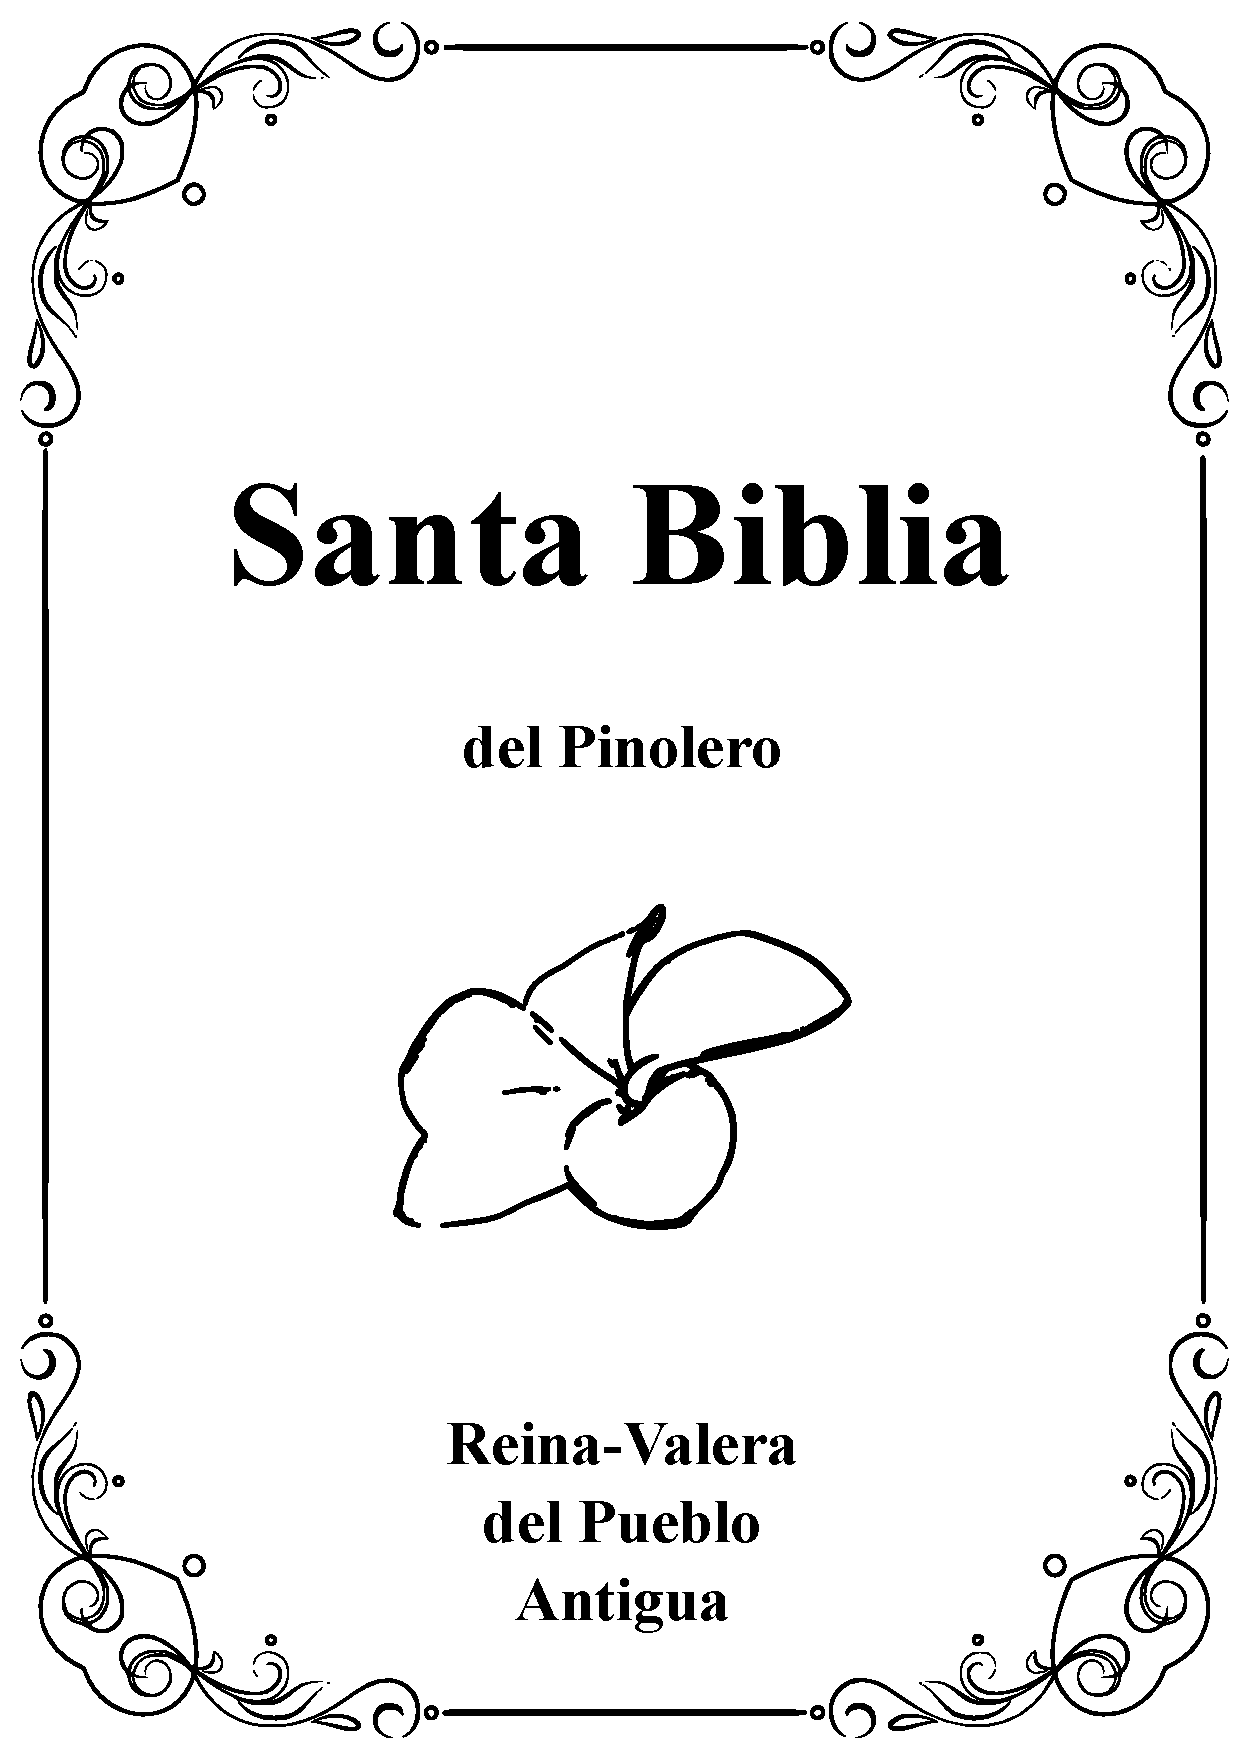
\includepdf{HardCover.pdf}

\null\vfill
Reina-Valera 1909\\
dominio publico y fuente abierta,\\
creado por el ministerio Biblia del Pueblo\\
~\\
1ra edición 2021\\
~\\
ISBN \dots\\
~\\
\emph{Distribucion en Nicaragua}\\
Estrellas de Esperanza\\
Reparto santa Rosa de donde fue la hielera del yanki\\
media cuadra al sur o vien de donde es la carpinteria\\
media al sur casa color celeste\\
43000 Granada\\
Nicaragua\\
ventas@estrellasdeesperanza.org\\
www.estrellasdeesperanza.org\\
fb.me/biblia.del.pueblo\\
~\\
Derechos dominio publico, el texto de la Biblia es fuente abierta\\
con una licencia de Creative Commons Zero Licensce.\\
El código fuente de markdown y XeTeX se encuentra en github en\\
http://www.github.com/bibliadelpueblo/BibliaLibre\\
~\\
Imprenta: Imprenta Jigatsa, Managua, Nicaragua\\

\newpage

\null\vfill
\begin{center}
\begin{minipage}[c]{\textwidth}
  \begin{center}
  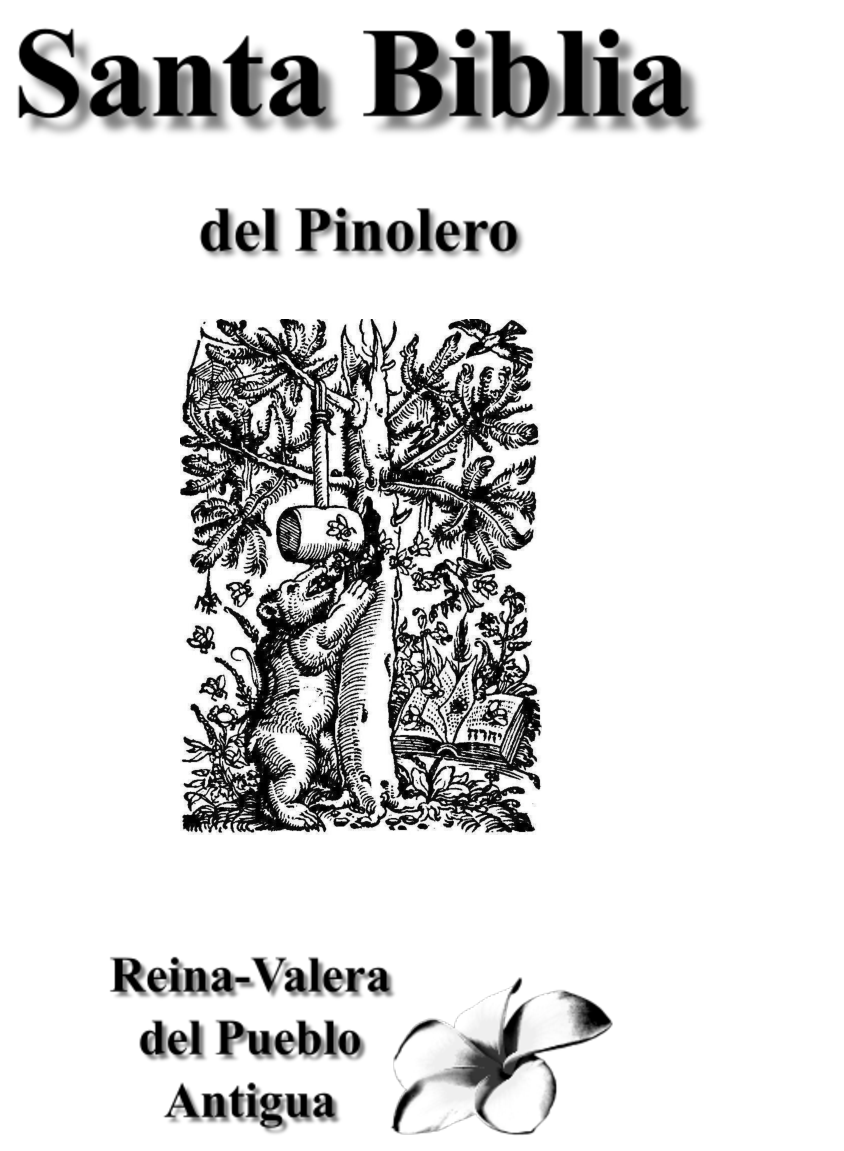
\includegraphics{Titel.pdf}
  \end{center}
\end{minipage}
\end{center}
\newpage



\titleformat{\section}[hang]{\bfseries\huge}{}{0ex}{}[]
\hypertarget{la-biblia-del-pinolero}{%
\section{La Biblia del Pinolero}\label{la-biblia-del-pinolero}}

Ese Biblia fue creado por la necesidad de los gentes en mucho países
latinos, que no pueden comprar una Biblia por causa del precio. Los
precios de las Biblias Reina-Valera en los países latinos son igual como
los precios en Europa o Estados Unidos, pero el salario medio es una
fracción. Hay muchas Biblias gratis, como de los Gedeones o de los
Moravias, o otro Biblias mas baratas, como la Nueva Version
Internacional, pero la traducción Reina-Valera es superior, y los
Biblias gratis tienen muchos desventajas. Problema, que los países
pobres no impriman Biblias es porque los textos de las traducciones son
protegido con derechos del autor. Por eso, los países pobres necesitan
una revisión de la Reina-Velara que es dominio publico y fuente abierta,
como se sabe eso del dominio de software, para que cada país, Casa
Editoral, organización, ministerio o Librería puede imprimir ese Biblia
y venderlo por precio mas barato. Por ahorita ese Biblia utiliza el
texto Reina-Valera 1909, pero vamos a hacer una revisión de dominio
publico y fuente abierta de castellano contemporáneo.

\hypertarget{trabajo-por-indigentes}{%
\section{Trabajo por Indigentes}\label{trabajo-por-indigentes}}

La idea de ese Biblia también es, dar trabajo a indigentes y pobres.
Cada ministerio que ayuda a indigentes y pobres puedes ofrecer trabajo
como vender ese Biblia en la calle, en buses etc., igual como un
periódico callejero que venden los indigentes. Se puede hacer así, que
los indigentes pueden recibir diez Biblias gratis para venderlos, y
después ellos pueden cargar doble el precio que pagan por ese Biblia en
el ministerio para venderlo. También, se puede cargar un diezmo de los
indigentes.

\hypertarget{solo-un-libro-o-palabra-de-dios}{%
\section{Solo un libro, o palabra de
Dios?}\label{solo-un-libro-o-palabra-de-dios}}

Hay dos razones porque sabemos que la Biblia es la palabra inspirada de
Dios. Dice Jesús que van venir muchos profetas falsos en su nombre y van
a engañar muchos. Y dice: ``Por sus frutos los conoceréis.'' Se mira,
que la Biblia es la palabra de Dios por los frutos de las vidas de los
autores, como los profetas o los apóstoles. Ellos hacen mucho milagros,
sanan leprosos, ciegos, paralizados, resucitan muertos y ayudan mucho a
los pobres. Eso son frutas de la verdad de Dios. No se hace milagros
así, si Dios no confirme las palabras de ese gente. Por eso sabemos que
Dios habla por las escrituras de ese gente. La otra razón porque sabemos
que la Biblia es la palabra de Dios es la sabiduría de las palabras de
Jesús, que supera cada sabiduría humana. Dice Jesús ``mis palabras son
espíritu y vida.'' Una vez yo recibe un alcohólico que se llama Daniel
para vivir en mi apartamiento, porque ello falta lugar para vivir. Yo lo
regalo una Biblia y dice: ``Lee esto!'' Ello me responde ``Nooo! No soy
permitido leer eso, solo el pastor es permitido!'', porque era un alemán
de Polonia, y en Polonia los pastores dicen que solo el Pastor es
permitido leer la Biblia. Yo digo a ese muchacho ``Tu es un pastor! Y
ahorita lees ese libro!''. Después ello comenzó leer ese Biblia como un
loco. Ello leo su Biblia por 3 horas diario, cada vez yo lo encuentra en
el parque era leyendo su Biblia. Dos meses mas, y ese alcohólico viene a
mi y me dice: ``Sabes, yo dejo beber Alcohol\ldots{}'' Yo digo ``Como?
Tu dejes beber Alcohol? Como tu haces eso? Tu no visitas nada Narcóticos
Anónimos, ni Doce Pasos, nada, como tu haces eso?'' ``No se, yo solo
dejo beber alcohol!'' Hay? En dos meses? Solo como leyendo su Biblia por
tres horas diario? Miran, eso es el poder de la Biblia, porque la Biblia
es espíritu y vida, y la Biblia tiene poder sanar un Alcohólico en dos
meses. Muchos gentes piensan que el poder de Dios sea en el fe. Eso es
así, pero solamente el fe no tiene poder, el poder viene de la verdad y
de vivir según la verdad. Es la verdad que tiene poder, no el fe. Por
eso, la Biblia tiene poder. Es imposible que Dios sea mentiroso. Dice
Jesús, ``Empero más fácil cosa es pasar el cielo y la tierra, que
frustrarse un tilde de la ley.'' Y por eso, cuando la palabra de Dios es
en nuestra boca, y nosotros cumplimos los requisitos de ese palabra,
Dios vas hacerlo. Mismo Jesús como hijo de Dios necesita luchar así,
cuando era confrontado con Satanás personalmente, Jesús siempre responde
a Satanás ``Escrito esta \ldots{}''. También por eso sabemos que la
Biblia es la palabra de Dios, porque eso es que enseña Jesús sobre las
escrituras. Mucho gente tambien acusan al Cristianismo que el
Crsitianismo no sea científico, y que ellos solo creen cosas que se
pruevan con Ciencia. Ese gente no entienden cual es Ciencia. Ciencias
Naturales functionan asi, que alguien crea una hipótesis. Para saber si
ese hipótesis sea verdad, necesita hacer experimentos y probar o
rechazar la hipóthesis con experimentos. Exacto eso es que se hace con
la Biblia como Cristiano, es exacto el mismo que hace la Ciencia. Nadie
en ese mundo solo cree en la Biblia por una decision de un dia a l'otro.
Con la Biblia se hace experimentos, se prueba las cosas, y por
experencia de milagros supernaturales se cresce fe, que la Biblia es la
verdad de Dios y que la Biblia functiona en su vida, en su vida
personal.

\hypertarget{como-leer-la-biblia}{%
\section{Como leer la Biblia}\label{como-leer-la-biblia}}

Para comenzar leer la Biblia es el mejor comenzar con el libro de Juan
en el Nuevo Testamento, porque en ese libro Jesús habla mucho, y se hace
conoscer Jesús el mas rapido. La Biblia es un libro que se lee diario, y
si solo son 5 minutos en la mañana. Dice la Biblia en Juan 6:
\bibverse{26} Respondióles Jesús, y dijo; De cierto, de cierto os digo,
que me buscáis, no porque habéis visto las señales, sino porque
comisteis el pan y os hartasteis.

\bibverse{27} Trabajad no por la comida que perece, mas por la comida
que á vida eterna permanece, la cual el Hijo del hombre os dará: porque
á éste señaló el Padre, que es Dios.

\bibverse{28} Y dijéronle: ¿Qué haremos para que obremos las obras de
Dios? \bibverse{29} Respondió Jesús, y díjoles: Esta es la obra de Dios,
que creáis en el que él ha enviado. \bibverse{30} Dijéronle entonces:
¿Qué señal pues haces tú, para que veamos, y te creamos? ¿Qué obras?
\bibverse{31} Nuestros padres comieron el maná en el desierto, como está
escrito: Pan del cielo les dió á comer. \bibverse{32} Y Jesús les dijo:
De cierto, de cierto os digo: No os dió Moisés pan del cielo; mas mi
Padre os da el verdadero pan del cielo. \bibverse{33} Porque el pan de
Dios es aquel que descendió del cielo y da vida al mundo. \bibverse{34}
Y dijéronle: Señor, danos siempre este pan. \bibverse{35} Y Jesús les
dijo: Yo soy el pan de vida: el que á mí viene, nunca tendrá hambre; y
el que en mí cree, no tendrá sed jamás.'' El maná fue el pan que los
israelitas comen en el desierto, cuando salieron de Egipto. El maná fue
necesario recoger diario para comer, así es el maná y pan de la Biblia.
Dice Jesús en Juan 8,31: ``Si vosotros permaneciereis en mi palabra,
seréis verdaderamente mis discípulos; Y conoceréis la verdad, y la
verdad os libertará.''. Entonces Jesús enseña leer su Biblia diario. La
Biblia también es un libro que da mucho consolación. Si estas triste,
leen Salmos o Isaías.

\hypertarget{como-la-biblia-fue-creado}{%
\section{Como la Biblia fue creado}\label{como-la-biblia-fue-creado}}

La Biblia normalmente consiste de 66 libros. El Anciano Testamento fue
escrito en hebreo de Moisés, Arón, Josué y todas las profetas. El Nuevo
Testamento fue escrito de los apóstoles como Pablo, Juan y Pedro en
griego. En tiempos antiguas, no había imprentas para imprimir libros,
entonces, los manuscritos fuesen reproducido por monjes en abadías por
muchos siglos. En el tiempo antes la reformacion un alemán Johannes
Gutenberg inventa imprimir libros con imprenta de tipos móviles. Con el
movimiento de la reformacion protestante, los Cristianos comenzan
traducir la Biblia en muchos idiomas. Mucho misioneros andan por países
lejos, y traducen la Biblia por su gente.

\hypertarget{la-biblia-reina-valera}{%
\section{La Biblia Reina Valera}\label{la-biblia-reina-valera}}

La Biblia Reina Valera era traducido de dos personas, de Casidoro De
Reina y Cipriano De Valera. Casidoro De Reina era un monje de Sevilla,
que acepta la reformacion protestante, y por eso ello necesita
refugiarse por otro país. Reina traduce la Biblia por Español en el año
1569, y ese Biblia fue imprimido en Basilea, Suiza y se llama La Biblia
del Oso. Mas tarde Cipriano Valera hace una revisión de la Biblia de
Reina. Su Biblia fue imprimido en Amsterdam en paises bajos y se llama
La Biblia del Cantaro en el año 1602.

\hypertarget{ministerio-biblia-del-pueblo}{%
\section{Ministerio Biblia del
Pueblo}\label{ministerio-biblia-del-pueblo}}

El Ministerio Biblia del Pueblo es un ministerio que hace revisiones de
textos bíblicos y biblias de dominio publico y fuente abierta en varios
idiomas y países. Biblia del Pueblo fue fundada 2021 en Granada,
Nicaragua.

\titleformat{\section}[wrap]{\bfseries\huge}{}{0ex}{}[]

\tableofcontents
\newpage

\null\vfill
\begin{center}
\begin{minipage}[c]{\textwidth}
  \begin{center}
  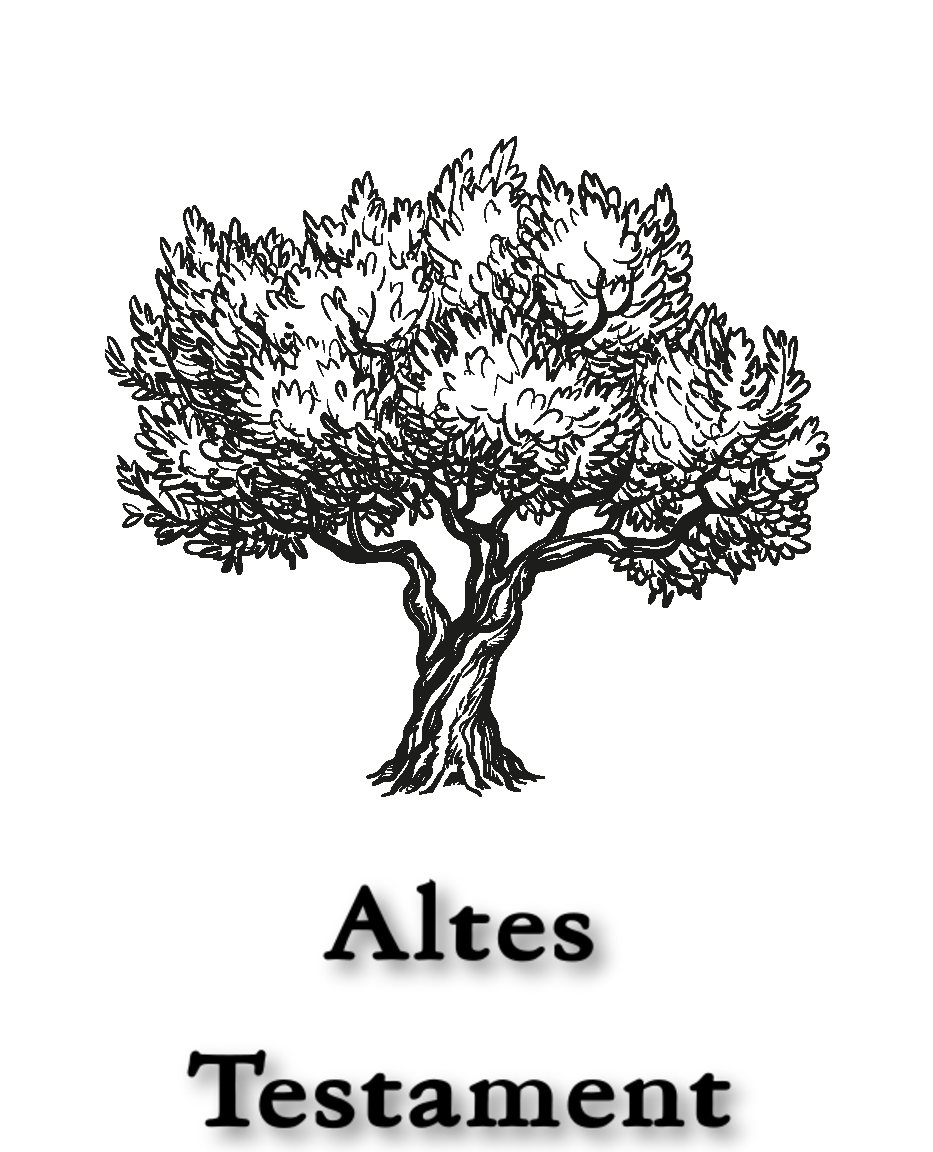
\includegraphics{AltesTestamentTitel.pdf}
  \end{center}
\end{minipage}
\end{center}
\null\vfill
\newpage

\pagestyle{bible}

\renewcommand{\cleardoublepage}{}
\renewcommand{\clearpage}{}

\chapter{1. Mose}
\begin{multicols}{2}
  \hypertarget{section}{%
\section{1}\label{section}}

\bibleverse{1} Am Anfang schuf Gott Himmel und Erde. \bibleverse{2} Und
die Erde war wüst und leer, und es war finster auf der Tiefe; und der
Geist Gottes schwebte auf dem Wasser. \bibleverse{3} Und Gott sprach: Es
werde Licht! und es ward Licht. \bibleverse{4} Und Gott sah, dass das
Licht gut war. Da schied Gott das Licht von der Finsternis
\bibleverse{5} und nannte das Licht Tag und die Finsternis Nacht. Da
ward aus Abend und Morgen der erste Tag.

\bibleverse{6} Und Gott sprach: Es werde eine Feste zwischen den
Wassern, und die sei ein Unterschied zwischen den Wassern.
\bibleverse{7} Da machte Gott die Feste und schied das Wasser unter der
Feste von dem Wasser über der Feste. Und es geschah also. \bibleverse{8}
Und Gott nannte die Feste Himmel. Da ward aus Abend und Morgen der
zweite Tag. \bibleverse{9} Und Gott sprach: Es sammle sich das Wasser
unter dem Himmel an besondere Örter, dass man das Trockene sehe. Und es
geschah also. \bibleverse{10} Und Gott nannte das Trockene Erde, und die
Sammlung der Wasser nannte er Meer. Und Gott sah, dass es gut war.
\bibleverse{11} Und Gott sprach: Es lasse die Erde aufgehen Gras und
Kraut, das sich besame, und fruchtbare Bäume, da ein jeglicher nach
seiner Art Frucht trage und habe seinen eigenen Samen bei sich selbst
auf Erden. Und es geschah also. \bibleverse{12} Und die Erde ließ
aufgehen Gras und Kraut, das sich besamte, ein jegliches nach seiner
Art, und Bäume, die da Frucht trugen und ihren eigenen Samen bei sich
selbst hatten, ein jeglicher nach seiner Art. Und Gott sah, dass es gut
war. \bibleverse{13} Da ward aus Abend und Morgen der dritte Tag.

\bibleverse{14} Und Gott sprach: Es werden Lichter an der Feste des
Himmels, die da scheiden Tag und Nacht und geben Zeichen, Zeiten, Tage
und Jahre \bibleverse{15} und seien Lichter an der Feste des Himmels,
dass sie scheinen auf Erden. Und es geschah also. \bibleverse{16} Und
Gott machte zwei große Lichter: ein großes Licht, das den Tag regiere,
und ein kleines Licht, das die Nacht regiere, dazu auch Sterne.
\bibleverse{17} Und Gott setzte sie an die Feste des Himmels, dass sie
schienen auf die Erde \bibleverse{18} und den Tag und die Nacht
regierten und schieden Licht und Finsternis. Und Gott sah, dass es gut
war. \bibleverse{19} Da ward aus Abend und Morgen der vierte Tag.
\bibleverse{20} Und Gott sprach: Es wimmle das Wasser von webenden und
lebendigen Tieren, und Gevögel fliege auf Erden unter der Feste des
Himmels. \bibleverse{21} Und Gott schuf große Walfische und allerlei
Getier, das da lebt und webt, davon das Wasser wimmelte, ein jegliches
nach seiner Art, und allerlei gefiedertes Gevögel, ein jegliches nach
seiner Art. Und Gott sah, dass es gut war. \bibleverse{22} Und Gott
segnete sie und sprach: Seid fruchtbar und mehret euch und erfüllt das
Wasser im Meer; und das Gefieder mehre sich auf Erden. \bibleverse{23}
Da ward aus Abend und Morgen der fünfte Tag.

\bibleverse{24} Und Gott sprach: Die Erde bringe hervor lebendige Tiere,
ein jegliches nach seiner Art: Vieh, Gewürm und Tiere auf Erden, ein
jegliches nach seiner Art. Und es geschah also. \bibleverse{25} Und Gott
machte die Tiere auf Erden, ein jegliches nach seiner Art, und das Vieh
nach seiner Art, und allerlei Gewürm auf Erden nach seiner Art. Und Gott
sah, dass es gut war.

\bibleverse{26} Und Gott sprach: Lasset uns Menschen machen, ein Bild,
das uns gleich sei, die da herrschen über die Fische im Meer und über
die Vögel unter dem Himmel und über das Vieh und über die ganze Erde und
über alles Gewürm, das auf Erden kriecht. \bibleverse{27} Und Gott schuf
den Menschen ihm zum Bilde, zum Bilde Gottes schuf er ihn; und schuf sie
einen Mann und eine Frau. \bibleverse{28} Und Gott segnete sie und
sprach zu ihnen: Seid fruchtbar und mehret euch und füllet die Erde und
machet sie euch untertan und herrschet über die Fische im Meer und über
die Vögel unter dem Himmel und über alles Getier, das auf Erden kriecht.
\bibleverse{29} Und Gott sprach: Seht da, ich habe euch gegeben allerlei
Kraut, das sich besamt, auf der ganzen Erde und allerlei fruchtbare
Bäume, die sich besamen, zu eurer Speise, \bibleverse{30} und allem
Getier auf Erden und allen Vögeln unter dem Himmel und allem Gewürm, das
da lebt auf Erden, dass sie allerlei grünes Kraut essen. Und es geschah
also. \bibleverse{31} Und Gott sah alles an, was er gemacht hatte; und
siehe da, es war sehr gut. Da ward aus Abend und Morgen der sechste Tag.

\hypertarget{section-1}{%
\section{2}\label{section-1}}

\bibleverse{1} Also ward vollendet Himmel und Erde mit ihrem ganzen
Heer. \bibleverse{2} Und also vollendete Gott am siebenten Tage seine
Werke, die er machte, und ruhte am siebenten Tage von allen seinen
Werken, die er machte. \bibleverse{3} Und Gott segnete den siebenten Tag
und heiligte ihn, darum dass er an demselben geruht hatte von allen
seinen Werken, die Gott schuf und machte. \bibleverse{4} Also ist Himmel
und Erde geworden, da sie geschaffen sind, zu der Zeit, da Gott der
\textsc{Herr} Erde und Himmel machte. \bibleverse{5} Und allerlei Bäume
auf dem Felde waren noch nicht auf Erden, und allerlei Kraut auf dem
Felde war noch nicht gewachsen; denn Gott der \textsc{Herr} hatte noch
nicht regnen lassen auf Erden, und es war kein Mensch, der das Land
bebaute. \bibleverse{6} Aber ein Nebel ging auf von der Erde und
feuchtete alles Land. \bibleverse{7} Und Gott der \textsc{Herr} machte
den Menschen aus einem Erdenkloß, und er blies ihm ein den lebendigen
Odem in seine Nase. Und also ward der Mensch eine lebendige Seele.
\bibleverse{8} Und Gott der \textsc{Herr} pflanzte einen Garten in Eden
gegen Morgen und setzte den Menschen hinein, den er gemacht hatte.
\bibleverse{9} Und Gott der \textsc{Herr} ließ aufwachsen aus der Erde
allerlei Bäume, lieblich anzusehen und gut zu essen, und den Baum des
Lebens mitten im Garten und den Baum der Erkenntnis des Guten und Bösen.
\bibleverse{10} Und es ging aus von Eden ein Strom, zu wässern den
Garten, und er teilte sich von da in vier Hauptwasser. \bibleverse{11}
Das erste heißt Pison, das fließt um das ganze Land Hevila; und daselbst
findet man Gold. \bibleverse{12} Und das Gold des Landes ist köstlich;
und da findet man Bedellion und den Edelstein Onyx. \bibleverse{13} Das
andere Wasser heißt Gihon, das fließt um um das ganze Mohrenland.
\bibleverse{14} Das dritte Wasser heißt Hiddekel, das fließt vor
Assyrien. Das vierte Wasser ist der Euphrat. \bibleverse{15} Und Gott
der \textsc{Herr} nahm den Menschen und setzte ihn in den Garten Eden,
dass er ihn baute und bewahrte. \bibleverse{16} Und Gott der
\textsc{Herr} gebot dem Menschen und sprach: Du sollst essen von
allerlei Bäumen im Garten; \bibleverse{17} aber von dem Baum der
Erkenntnis des Guten und Bösen sollst du nicht essen; denn welches Tages
du davon issest, wirst du des Todes sterben. \bibleverse{18} Und Gott
der \textsc{Herr} sprach: Es ist nicht gut, dass der Mensch allein sei;
ich will ihm eine Gehilfin machen, die um ihn sei. \bibleverse{19} Denn
als Gott der \textsc{Herr} gemacht hatte von der Erde allerlei Tiere auf
dem Felde und allerlei Vögel unter dem Himmel, brachte er sie zu dem
Menschen, dass er sähe, wie er sie nennte; denn wie der Mensch allerlei
lebendige Tiere nennen würde, so sollten sie heißen. \bibleverse{20} Und
der Mensch gab einem jeglichen Vieh und Vogel unter dem Himmel und Tier
auf dem Felde seinen Namen; aber für den Menschen ward keine Gehilfin
gefunden, die um ihn wäre. \bibleverse{21} Da ließ Gott der
\textsc{Herr} einen tiefen Schlaf fallen auf den Menschen, und er
schlief ein. Und er nahm eine seiner Rippen und schloss die Stätte zu
mit Fleisch. \bibleverse{22} Und Gott der \textsc{Herr} baute eine Frau
aus der Rippe, die er vom Menschen nahm, und brachte sie zu ihm.
\bibleverse{23} Da sprach der Mensch: Das ist doch Bein von meinem Bein
und Fleisch von meinem Fleisch; man wird sie Männin heißen, darum dass
sie vom Manne genommen ist. \bibleverse{24} Darum wird ein Mann Vater
und Mutter verlassen und an seiner Frau hangen, und sie werden sein ein
Fleisch. \bibleverse{25} Und sie waren beide nackt, der Mensch und seine
Frau, und schämten sich nicht.

\hypertarget{section-2}{%
\section{3}\label{section-2}}

\bibleverse{1} Und die Schlange war listiger denn alle Tiere auf dem
Felde, die Gott der \textsc{Herr} gemacht hatte, und sprach zu der Frau:
Ja, sollte Gott gesagt haben: Ihr sollt nicht essen von allerlei Bäumen
im Garten?

\bibleverse{2} Da sprach die Frau zu der Schlange: Wir essen von den
Früchten der Bäume im Garten; \bibleverse{3} aber von den Früchten des
Baumes mitten im Garten hat Gott gesagt: Esset nicht davon, rühret's
auch nicht an, dass ihr nicht sterbet. \bibleverse{4} Da sprach die
Schlange zur Frau: Ihr werdet mitnichten des Todes sterben;
\bibleverse{5} sondern Gott weiß, dass, welches Tages ihr davon esset,
so werden eure Augen aufgetan, und werdet sein wie Gott und wissen, was
gut und böse ist. \bibleverse{6} Und die Frau schaute an, dass von dem
Baum gut zu essen wäre und dass er lieblich anzusehen und ein lustiger
Baum wäre, weil er klug machte; und sie nahm von der Frucht und aß und
gab ihrem Mann auch davon, und er aß. \bibleverse{7} Da wurden ihrer
beider Augen aufgetan, und sie wurden gewahr, dass sie nackt waren, und
flochten Feigenblätter zusammen und machten sich Schürze. \bibleverse{8}
Und sie hörten die Stimme Gottes des \textsc{Herrn}, der im Garten ging,
da der Tag kühl geworden war. Und Adam versteckte sich mit seiner Frau
vor dem Angesicht Gottes des \textsc{Herrn} unter die Bäume im Garten.
\bibleverse{9} Und Gott der \textsc{Herr} rief Adam und sprach zu ihm:
Wo bist du?

\bibleverse{10} Und er sprach: Ich hörte deine Stimme im Garten und
fürchtete mich; denn ich bin nackt, darum versteckte ich mich.

\bibleverse{11} Und er sprach: Wer hat dir's gesagt, dass du nackt bist?
Hast du nicht gegessen von dem Baum, davon ich dir gebot, du solltest
nicht davon essen?

\bibleverse{12} Da sprach Adam: Die Frau, die du mir zugesellt hast, gab
mir von dem Baum, und ich aß.

\bibleverse{13} Da sprach Gott der \textsc{Herr} zur Frau: Warum hast du
das getan? Die Frau sprach: Die Schlange betrog mich also, dass ich aß.
\bibleverse{14} Da sprach Gott der \textsc{Herr} zu der Schlange: Weil
du solches getan hast, seist du verflucht vor allem Vieh und vor allen
Tieren auf dem Felde. Auf deinem Bauche sollst du gehen und Erde essen
dein Leben lang. \bibleverse{15} Und ich will Feindschaft setzen
zwischen dir und der Frau und zwischen deinem Samen und ihrem Samen.
Derselbe soll dir den Kopf zertreten, und du wirst ihn in die Ferse
stechen. \bibleverse{16} Und zur Frau sprach er: Ich will dir viel
Schmerzen schaffen, wenn du schwanger wirst; du sollst mit Schmerzen
Kinder gebären; und dein Verlangen soll nach deinem Manne sein, und er
soll dein Herr sein. \bibleverse{17} Und zu Adam sprach er: Dieweil du
hast gehorcht der Stimme deiner Frau und hast gegessen von dem Baum,
davon ich dir gebot und sprach: Du sollst nicht davon essen, --
verflucht sei der Acker um deinetwillen, mit Kummer sollst du dich
darauf nähren dein Leben lang. \bibleverse{18} Dornen und Disteln soll
er dir tragen, und sollst das Kraut auf dem Felde essen. \bibleverse{19}
Im Schweiße deines Angesichts sollst du dein Brot essen, bis dass du
wieder zu Erde werdest, davon du genommen bist. Denn du bist Erde und
sollst zu Erde werden. \bibleverse{20} Und Adam hieß seine Frau Eva,
darum dass sie eine Mutter ist aller Lebendigen. \bibleverse{21} Und
Gott der \textsc{Herr} machte Adam und seiner Frau Röcke von Fellen und
kleidete sie.

\bibleverse{22} Und Gott der \textsc{Herr} sprach: Siehe, Adam ist
geworden wie unsereiner und weiß, was gut und böse ist. Nun aber, dass
er nicht ausstrecke seine Hand und breche auch von dem Baum des Lebens
und esse und lebe ewiglich! \bibleverse{23} Da wies ihn Gott der
\textsc{Herr} aus dem Garten Eden, dass er das Feld baute, davon er
genommen ist, \bibleverse{24} und trieb Adam aus und lagerte vor den
Garten Eden die Cherubim mit dem bloßen, feurigen Schwert, zu bewahren
den Weg zu dem Baum des Lebens.

\hypertarget{section-3}{%
\section{4}\label{section-3}}

\bibleverse{1} Und Adam erkannte seine Frau Eva, und sie ward schwanger
und gebar den Kain und sprach: Ich habe einen Mann gewonnen mit dem
\textsc{Herrn}. \bibleverse{2} Und sie fuhr fort und gebar Abel, seinen
Bruder. Und Abel ward ein Schäfer; Kain aber ward ein Ackermann.
\bibleverse{3} Es begab sich aber nach etlicher Zeit, dass Kain dem
\textsc{Herrn} Opfer brachte von den Früchten des Feldes; \bibleverse{4}
und Abel brachte auch von den Erstlingen seiner Herde und von ihrem
Fett. Und der \textsc{Herr} sah gnädig an Abel und sein Opfer;
\bibleverse{5} aber Kain und sein Opfer sah er nicht gnädig an. Da
ergrimmte Kain sehr, und sein Blick senkte sich. \bibleverse{6} Da
sprach der \textsc{Herr} zu Kain: Warum ergrimmst du? und warum senkt
sich deine Blick? \bibleverse{7} Ist's nicht also? Wenn du gutes tust,
so bist du angenehm; tust du aber böses, so ruht die Sünde vor der Tür,
und nach dir hat sie Verlangen; du aber herrsche über sie.
\bibleverse{8} Da redete Kain mit seinem Bruder Abel. Und es begab sich,
da sie auf dem Felde waren, erhob sich Kain wider seinen Bruder Abel und
schlug ihn tot. \bibleverse{9} Da sprach der \textsc{Herr} zu Kain: Wo
ist dein Bruder Abel? Er sprach: Ich weiß nicht; soll ich meines Bruders
Hüter sein?

\bibleverse{10} Er aber sprach: Was hast du getan? Die Stimme des Bluts
deines Bruders schreit zu mir von der Erde. \bibleverse{11} Und nun
verflucht seist du auf der Erde, die ihr Maul hat aufgetan und deines
Bruders Blut von deinen Händen empfangen. \bibleverse{12} Wenn du den
Acker bauen wirst, soll er dir hinfort seinen Ertrag nicht geben. Unstet
und flüchtig sollst du sein auf Erden.

\bibleverse{13} Kain aber sprach zu dem \textsc{Herrn}: Meine Sünde ist
größer, denn dass sie mir vergeben werden möge. \bibleverse{14} Siehe,
du treibst mich heute aus dem Lande, und ich muss mich vor deinem
Angesicht verbergen und muss unstet und flüchtig sein auf Erden. So wird
mir's gehen, dass mich totschlage, wer mich findet.

\bibleverse{15} Aber der \textsc{Herr} sprach zu ihm: Nein; sondern wer
Kain totschlägt, das soll siebenfältig gerächt werden. Und der
\textsc{Herr} machte ein Zeichen an Kain, dass ihn niemand erschlüge,
wer ihn fände.

\bibleverse{16} Also ging Kain von dem Angesicht des \textsc{Herrn} und
wohnte im Lande Nod, jenseits Eden, gegen Morgen. \bibleverse{17} Und
Kain erkannte seine Frau, die ward schwanger und gebar den Henoch. Und
er baute eine Stadt, die nannte er nach seines Sohnes Namen Henoch.
\bibleverse{18} Henoch aber zeugte Irad, Irad zeugte Mahujael, Mahujael
zeugte Methusael, Methusael zeugte Lamech. \bibleverse{19} Lamech aber
nahm zwei Frauen; eine hieß Ada, die andere Zilla. \bibleverse{20} Und
Ada gebar Jabal; von dem sind hergekommen, die in Hütten wohnten und
Vieh zogen. \bibleverse{21} Und sein Bruder hieß Jubal; von dem sind
hergekommen die Geiger und Pfeifer. \bibleverse{22} Die Zilla aber gebar
auch, nämlich den Thubalkain, den Meister in allerlei Erz- und
Eisenwerk. Und die Schwester des Thubalkain war Naema. \bibleverse{23}
Und Lamech sprach zu seinen Frauen Ada und Zilla: Ihr Frauen Lamechs,
höret meine Rede und merket, was ich sage: Ich habe einen Mann
erschlagen für meine Wunde und einen Jüngling für meine Beule;
\bibleverse{24} Kain soll siebenmal gerächt werden, aber Lamech
siebenundsiebzigmal. \bibleverse{25} Adam erkannte abermals seine Frau,
und sie gebar einen Sohn, den hieß sie Seth; denn Gott hat mir, sprach
sie, einen anderen Samen gesetzt für Abel, den Kain erwürgt hat.
\bibleverse{26} Und Seth zeugte auch einen Sohn und hieß ihn Enos. Zu
der Zeit fing man an, den Namen des \textsc{Herrn} anzurufen.

\hypertarget{section-4}{%
\section{5}\label{section-4}}

\bibleverse{1} Dies ist das Buch von des Menschen Geschlecht. Da Gott
den Menschen schuf, machte er ihn nach dem Bilde Gottes; \bibleverse{2}
und schuf sie einen Mann und eine Frau und segnete sie und hieß ihren
Namen Mensch zur Zeit, da sie geschaffen wurden. \bibleverse{3} Und Adam
war 130 Jahre alt und zeugte einen Sohn, der seinem Bild ähnlich war und
hieß ihn Seth \bibleverse{4} und lebte danach 800 Jahre und zeugte Söhne
und Töchter; \bibleverse{5} dass sein ganzes Alter ward 930 Jahre, und
starb. \bibleverse{6} Seth war 105 Jahre alt und zeugte Enos
\bibleverse{7} und lebte danach 807 Jahre und zeugte Söhne und Töchter;
\bibleverse{8} dass sein ganzes Alter ward 912 Jahre, und starb.

\bibleverse{9} Enos war 90 Jahre alt und zeugte Kenan \bibleverse{10}
und lebte danach 815 Jahre und zeugte Söhne und Töchter; \bibleverse{11}
dass sein ganzes Alter ward 905 Jahre, und starb.

\bibleverse{12} Kenan war 70 Jahre alt und zeugte Mahalaleel
\bibleverse{13} und lebte danach 840 Jahre und zeugte Söhne und Töchter;
\bibleverse{14} dass sein ganzes Alter ward 910 Jahre, und starb.

\bibleverse{15} Mahalaleel war 65 Jahre alt und zeugte Jared
\bibleverse{16} und lebte danach 830 Jahre und zeugte Söhne und Töchter;
\bibleverse{17} dass sein ganzes Alter ward 895 Jahre, und starb.

\bibleverse{18} Jared war 162 Jahre alt und zeugte Henoch
\bibleverse{19} und er lebte danach 800 Jahre und zeugte Söhne und
Töchter; \bibleverse{20} dass sein ganzes Alter ward 962 Jahre, und
starb.

\bibleverse{21} Henoch war 65 Jahre alt und zeugte Methusalah.
\bibleverse{22} Und nachdem er Methusalah gezeugt hatte, blieb er in
einem göttlichen Leben 300 Jahre und zeugte Söhne und Töchter;
\bibleverse{23} dass sein ganzes Alter ward 365 Jahre. \bibleverse{24}
Und weil er ein göttliches Leben führte, nahm ihn Gott hinweg, und er
ward nicht mehr gesehen. \bibleverse{25} Methusalah war 187 Jahre alt
und zeugte Lamech \bibleverse{26} und lebte danach 782 Jahre und zeugte
Söhne und Töchter; \bibleverse{27} dass sein ganzes Alter ward 969
Jahre, und starb.

\bibleverse{28} Lamech war 182 Jahre alt und zeugte einen Sohn
\bibleverse{29} und hieß ihn Noah und sprach: Der wird uns trösten in
unserer Mühe und Arbeit auf der Erde, die der \textsc{Herr} verflucht
hat. \bibleverse{30} Danach lebte er 595 Jahre und zeugte Söhne und
Töchter; \bibleverse{31} dass sein ganzes Alter ward 777 Jahre, und
starb. \bibleverse{32} Noah war 500 Jahre alt und zeugte Sem, Ham und
Japheth.

\hypertarget{section-5}{%
\section{6}\label{section-5}}

\bibleverse{1} Da sich aber die Menschen begannen zu mehren auf Erden
und ihnen Töchter geboren wurden, \bibleverse{2} da sahen die Kinder
Gottes nach den Töchtern der Menschen, wie sie schön waren, und nahmen
zu Frauen, welche sie wollten. \bibleverse{3} Da sprach der
\textsc{Herr}: Die Menschen wollen sich von meinem Geist nicht mehr
strafen lassen; denn sie sind Fleisch. Ich will ihnen noch Frist geben
120 Jahre. \bibleverse{4} Es waren auch zu den Zeiten Tyrannen auf
Erden; denn da die „Kinder Gottes`` zu den „Töchtern der Menschen``
eingingen und sie ihnen Kinder gebaren, wurden daraus Gewaltige in der
Welt und berühmte Männer. \bibleverse{5} Da aber der \textsc{Herr} sah,
dass der Menschen Bosheit groß war auf Erden und alles Dichten und
Trachten ihres Herzens nur böse war immerdar, \bibleverse{6} da reute es
ihn, dass er die Menschen gemacht hatte auf Erden, und es bekümmerte ihn
in seinem Herzen, \bibleverse{7} und er sprach: Ich will die Menschen,
die ich geschaffen habe, vertilgen von der Erde, vom Menschen an bis auf
das Vieh und bis auf das Gewürm und bis auf die Vögel unter dem Himmel;
denn es reut mich, dass ich sie gemacht habe. \bibleverse{8} Aber Noah
fand Gnade vor dem \textsc{Herrn}. \bibleverse{9} Dies ist das
Geschlecht Noahs. Noah war ein frommer Mann und ohne Tadel und führte
ein göttliches Leben zu seinen Zeiten \bibleverse{10} und zeugte drei
Söhne: Sem, Ham und Japheth. \bibleverse{11} Aber die Erde war verderbt
vor Gottes Augen und voll Frevels. \bibleverse{12} Da sah Gott auf die
Erde, und siehe, sie war verderbt; denn alles Fleisch hatte seinen Weg
verderbt auf Erden. \bibleverse{13} Da sprach Gott zu Noah: Alles
Fleisches Ende ist vor mich gekommen; denn die Erde ist voll Frevels von
ihnen; und siehe da, ich will sie verderben mit der Erde.
\bibleverse{14} Mache dir eine Arche von Tannenholz und mache Kammern
darin und verpiche ihn mit Pech inwendig und auswendig. \bibleverse{15}
Und mache sie also: 300 Ellen sei die Länge, 50 Ellen die Weite und 30
Ellen die Höhe. \bibleverse{16} Ein Fenster sollst du daran machen
obenan, eine Elle groß. Die Tür sollst du mitten in ihre Seite setzen.
Und sie soll drei Boden haben: einen unten, den anderen in der Mitte,
den dritten in der Höhe. \bibleverse{17} Denn siehe, ich will eine
Sintflut mit Wasser kommen lassen auf Erden, zu verderben alles Fleisch,
darin ein lebendiger Odem ist, unter dem Himmel. Alles, was auf Erden
ist, soll untergehen. \bibleverse{18} Aber mit dir will ich einen Bund
aufrichten; und du sollst in die Arche gehen mit deinen Söhnen, mit
deiner Frau und mit deiner Söhne Frauen. \bibleverse{19} Und du sollst
in die Arche tun allerlei Tiere von allem Fleisch, je ein Paar, Männlein
und Weiblein, dass sie lebendig bleiben bei dir. \bibleverse{20} Von den
Vögeln nach ihrer Art, von dem Vieh nach seiner Art und von allerlei
Gewürm auf Erden nach seiner Art: von den allen soll je ein Paar zu dir
hineingehen, dass sie leben bleiben. \bibleverse{21} Und du sollst
allerlei Speise zu dir nehmen, die man isst, und sollst sie bei dir
sammeln, dass sie dir und ihnen zur Nahrung da sei. \bibleverse{22} Und
Noah tat alles, was ihm Gott gebot.

\hypertarget{section-6}{%
\section{7}\label{section-6}}

\bibleverse{1} Und der \textsc{Herr} sprach zu Noah: Gehe in die Arche,
du und dein ganzes Haus; denn ich habe dich gerecht ersehen vor mir zu
dieser Zeit. \bibleverse{2} Aus allerlei reinem Vieh nimm zu dir je
sieben und sieben, das Männlein und sein Weiblein; von dem unreinen Vieh
aber je ein Paar, das Männlein und sein Weiblein. \bibleverse{3}
Desgleichen von den Vögeln unter dem Himmel je sieben und sieben, das
Männlein und sein Weiblein, auf dass Same lebendig bleibe auf dem ganzen
Erdboden. \bibleverse{4} Denn von nun an über sieben Tage will ich
regnen lassen auf Erden 40 Tage und 40 Nächte und vertilgen von dem
Erdboden alles, was Odem hat, was ich gemacht habe. \bibleverse{5} Und
Noah tat alles, was ihm der \textsc{Herr} gebot.

\bibleverse{6} Er war aber 600 Jahre alt, da das Wasser der Sintflut auf
Erden kam. \bibleverse{7} Und er ging in die Arche mit seinen Söhnen,
seiner Frau und seiner Söhne Frauen vor dem Gewässer der Sintflut.
\bibleverse{8} Von dem reinen Vieh und von dem unreinen, von den Vögeln
und von allem Gewürm auf Erden \bibleverse{9} gingen zu ihm in die Arche
paarweise, je ein Männlein und Weiblein, wie ihm Gott geboten hatte.
\bibleverse{10} Und da die sieben Tage vergangen waren, kam das Gewässer
der Sintflut auf Erden. \bibleverse{11} In dem 601. Jahr des Alters
Noahs, am 17. Tage des zweiten Monats, das ist der Tag, da aufbrachen
alle Brunnen der großen Tiefe, und taten sich auf die Fenster des
Himmels, \bibleverse{12} und kam ein Regen auf Erden 40 Tage und 40
Nächte. \bibleverse{13} Eben am selben Tage ging Noah in die Arche mit
Sem, Ham und Japheth, seinen Söhnen, und mit seiner Frau und seiner
Söhne drei Frauen, \bibleverse{14} dazu allerlei Getier nach seiner Art,
allerlei Vieh nach seiner Art, allerlei Gewürm, das auf Erden kriecht,
nach seiner Art und allerlei Vögel nach ihrer Art, alles was fliegen
konnte, alles, was Fittiche hatte; \bibleverse{15} das ging alles zu
Noah in die Arche paarweise, von allem Fleisch, darin ein lebendiger
Geist war. \bibleverse{16} Und das waren Männlein und Weiblein von
allerlei Fleisch, und gingen hinein, wie denn Gott ihm geboten hatte.
Und der \textsc{Herr} schloss hinter ihm zu. \bibleverse{17} Da kam die
Sintflut 40 Tage auf Erden, und die Wasser wuchsen und hoben die Arche
auf und trugen sie empor über die Erde. \bibleverse{18} Also nahm das
Gewässer überhand und wuchs sehr auf Erden, dass die Arche auf dem
Gewässer fuhr. \bibleverse{19} Und das Gewässer nahm überhand und wuchs
so sehr auf Erden, dass alle hohen Berge unter dem ganzen Himmel bedeckt
wurden. \bibleverse{20} Fünfzehn Ellen hoch ging das Gewässer über die
Berge, die bedeckt wurden. \bibleverse{21} Da ging alles Fleisch unter,
das auf Erden kriecht, an Vögeln, an Vieh, an Tieren und an allem, was
sich regt auf Erden, und alle Menschen. \bibleverse{22} Alles, was einen
lebendigen Odem hatte auf dem Trockenen, das starb. \bibleverse{23} Also
ward vertilgt alles, was auf dem Erdboden war, vom Menschen an bis auf
das Vieh und das Gewürm und auf die Vögel unter dem Himmel; das ward
alles von der Erde vertilgt. Allein Noah blieb übrig und was mit ihm in
der Arche war. \bibleverse{24} Und das Gewässer stand auf Erden 150
Tage.

\hypertarget{section-7}{%
\section{8}\label{section-7}}

\bibleverse{1} Da gedachte Gott an Noah und an alle Tiere und an alles
Vieh, das mit ihm in der Arche war, und ließ Wind auf Erden kommen, und
die Wasser fielen; \bibleverse{2} und die Brunnen der Tiefe wurden
verstopft samt den Fenstern des Himmels, und dem Regen vom Himmel ward
gewehrt; \bibleverse{3} und das Gewässer verlief sich von der Erde immer
mehr und nahm ab nach 150 Tagen. \bibleverse{4} Am 17. Tage des
siebenten Monats ließ sich die Arche nieder auf das Gebirge Ararat.
\bibleverse{5} Es nahm aber das Gewässer immer mehr ab bis auf den
zehnten Monat. Am ersten Tage des zehnten Monats sahen der Berge Spitzen
hervor. \bibleverse{6} Nach 40 Tagen tat Noah das Fenster auf an der
Arche, das er gemacht hatte, \bibleverse{7} und ließ einen Raben
ausfliegen; der flog immer hin und wieder her, bis das Gewässer
vertrocknete auf Erden. \bibleverse{8} Danach ließ er eine Taube von
sich ausfliegen, auf dass er erführe, ob das Gewässer gefallen wäre auf
Erden. \bibleverse{9} Da aber die Taube nicht fand, da ihr Fuß ruhen
konnte, kam sie wieder zu ihm in die Arche; denn das Gewässer war noch
auf dem ganzen Erdboden. Da tat er die Hand heraus und nahm sie zu sich
in die Arche. \bibleverse{10} Da harrte er noch weitere sieben Tage und
ließ abermals eine Taube fliegen aus der Arche. \bibleverse{11} Die kam
zu ihm zur Abendzeit, und siehe, ein Ölblatt hatte sie abgebrochen und
trug's in ihrem Munde. Da merkte Noah, dass das Gewässer gefallen wäre
auf Erden. \bibleverse{12} Aber er harrte noch weitere sieben Tage und
ließ eine Taube ausfliegen; die kam nicht wieder zu ihm.

\bibleverse{13} Im 601. Jahr des Alters Noahs, am ersten Tage des ersten
Monats vertrocknete das Gewässer auf Erden. Da tat Noah das Dach von der
Arche und sah, dass der Erdboden trocken war. \bibleverse{14} Also ward
die Erde ganz trocken am 27. Tage des zweiten Monats.

\bibleverse{15} Da redete Gott mit Noah und sprach: \bibleverse{16} Gehe
aus der Arche, du und deine Frau, deine Söhne und deiner Söhne Frauen
mit dir. \bibleverse{17} Allerlei Getier, das bei dir ist, von allerlei
Fleisch, an Vögeln, an Vieh und an allerlei Gewürm, das auf Erden
kriecht, das gehe heraus mit dir, dass sie sich regen auf Erden und
fruchtbar seien und sich mehren auf Erden.

\bibleverse{18} Also ging Noah heraus mit seinen Söhnen und seiner Frau
und seiner Söhne Frauen, \bibleverse{19} dazu allerlei Getier, allerlei
Gewürm, allerlei Vögel und alles, was auf Erden kriecht; das ging aus
der Arche, ein jegliches mit seinesgleichen. \bibleverse{20} Noah aber
baute dem \textsc{Herrn} einen Altar und nahm von allerlei reinem Vieh
und von allerlei reinem Geflügel und opferte Brandopfer auf dem Altar.
\bibleverse{21} Und der \textsc{Herr} roch den lieblichen Geruch und
sprach in seinem Herzen: Ich will hinfort nicht mehr die Erde verfluchen
um der Menschen willen; denn das Dichten des menschlichen Herzens ist
böse von Jugend auf. Und ich will hinfort nicht mehr schlagen alles, was
da lebt, wie ich getan habe. \bibleverse{22} Solange die Erde steht,
soll nicht aufhören Saat und Ernte, Frost und Hitze, Sommer und Winter,
Tag und Nacht.

\hypertarget{section-8}{%
\section{9}\label{section-8}}

\bibleverse{1} Und Gott segnete Noah und seine Söhne und sprach: Seid
fruchtbar und mehret euch und erfüllet die Erde. \bibleverse{2} Furcht
und Schrecken vor euch sei über alle Tiere auf Erden und über alle Vögel
unter dem Himmel, über alles, was auf dem Erdboden kriecht, und über
alle Fische im Meer; in eure Hände seien sie gegeben. \bibleverse{3}
Alles, was sich regt und lebt, das sei eure Speise; wie das grüne Kraut
habe ich's euch alles gegeben. \bibleverse{4} Allein esset das Fleisch
nicht, das noch lebt in seinem Blut. \bibleverse{5} Auch will ich eures
Leibes Blut rächen und will's an allen Tieren rächen und will des
Menschen Leben rächen an einem jeglichen Menschen als dem, der sein
Bruder ist. \bibleverse{6} Wer Menschenblut vergießt, des Blut soll auch
durch Menschen vergossen werden; denn Gott hat den Menschen zu seinem
Bilde gemacht. \bibleverse{7} Seid fruchtbar und mehret euch und reget
euch auf Erden, dass euer viel darauf werden. \bibleverse{8} Und Gott
sagte zu Noah und seinen Söhnen mit ihm: \bibleverse{9} Siehe, ich
richte mit euch einen Bund auf und mit eurem Samen nach euch
\bibleverse{10} und mit allem lebendigen Getier bei euch, an Vögeln, an
Vieh und an allen Tieren auf Erden bei euch, von allem, was aus dem
Kasten gegangen ist, was für Tiere es sind auf Erden. \bibleverse{11}
Und ich richte meinen Bund also mit euch auf, dass hinfort nicht mehr
alles Fleisch verderbt soll werden mit dem Wasser der Sintflut, und soll
hinfort keine Sintflut mehr kommen, die die Erde verderbe.
\bibleverse{12} Und Gott sprach: Das ist das Zeichen des Bundes, den ich
gemacht habe zwischen mir und euch und allen lebendigen Seelen bei euch
hinfort ewiglich: \bibleverse{13} Meinen Bogen habe ich gesetzt in die
Wolken; der soll das Zeichen sein des Bundes zwischen mir und der Erde.
\bibleverse{14} Und wenn es kommt, dass ich Wolken über die Erde führe,
so soll man meinen Bogen sehen in den Wolken. \bibleverse{15} Alsdann
will ich gedenken an meinen Bund zwischen mir und euch und allen
lebendigen Seelen in allerlei Fleisch, dass nicht mehr hinfort eine
Sintflut komme, die alles Fleisch verderbe. \bibleverse{16} Darum soll
mein Bogen in den Wolken sein, dass ich ihn ansehe und gedenke an den
ewigen Bund zwischen Gott und allen lebendigen Seelen in allem Fleisch,
das auf Erden ist. \bibleverse{17} Und Gott sagte zu Noah: Das sei das
Zeichen des Bundes, den ich aufgerichtet habe zwischen mir und allem
Fleisch auf Erden. \bibleverse{18} Die Söhne Noahs, die aus dem Kasten
gingen, sind diese: Sem, Ham und Japheth. Ham aber ist der Vater
Kanaans. \bibleverse{19} Das sind die drei Söhne Noahs, von denen ist
alles Land besetzt.

\bibleverse{20} Noah aber fing an und ward ein Ackermann und pflanzte
Weinberge. \bibleverse{21} Und da er von dem Wein trank, ward er trunken
und lag in der Hütte aufgedeckt. \bibleverse{22} Da nun Ham, Kanaans
Vater, sah seines Vaters Blöße, sagte er's seinen beiden Brüdern
draußen. \bibleverse{23} Da nahmen Sem und Japheth ein Kleid und legten
es auf ihrer beider Schultern und gingen rücklings hinzu und deckten des
Vaters Blöße zu; und ihr Angesicht war abgewandt, dass sie ihres Vater
Blöße nicht sahen. \bibleverse{24} Als nun Noah erwachte von seinem Wein
und erfuhr, was ihm sein jüngster Sohn getan hatte, \bibleverse{25}
sprach er: Verflucht sei Kanaan und sei ein Knecht aller Knechte unter
seinen Brüdern! \bibleverse{26} und sprach weiter: Gelobt sei der
\textsc{Herr}, der Gott Sems; und Kanaan sei sein Knecht!
\bibleverse{27} Gott breite Japheth aus, und lasse ihn wohnen in den
Hütten des Sem; und Kanaan sei sein Knecht! \bibleverse{28} Noah aber
lebte nach der Sintflut 350 Jahre, \bibleverse{29} dass sein ganzes
Alter ward 950 Jahre, und starb.

\hypertarget{section-9}{%
\section{10}\label{section-9}}

\bibleverse{1} Dies ist das Geschlecht der Kinder Noahs: Sem, Ham,
Japheth. Und sie zeugten Kinder nach der Sintflut.

\bibleverse{2} Die Kinder Japheths sind diese: Gomer, Magog, Madai,
Javan, Thubal, Mesech und Thiras. \bibleverse{3} Aber die Kinder von
Gomer sind diese: Askenas, Riphath und Thogarma. \bibleverse{4} Die
Kinder von Javan sind diese: Elisa, Tharsis, die Chittiter und die
Dodaniter. \bibleverse{5} Von diesen sind ausgebreitet die Inseln der
Heiden in ihren Ländern, jegliche nach ihren Sprachen, Geschlechtern und
Leuten.

\bibleverse{6} Die Kinder von Ham sind diese: Kusch, Mizraim, Put und
Kanaan. \bibleverse{7} Aber die Kinder von Kusch sind diese: Seba,
Hevila, Sabtha, Ragma und Sabthecha. Aber die Kinder von Ragma sind
diese: Saba und Dedan. \bibleverse{8} Kusch aber zeugte den Nimrod. Der
fing an ein gewaltiger Herr zu sein auf Erden, \bibleverse{9} und war
ein gewaltiger Jäger vor dem \textsc{Herrn}. Daher spricht man: Das ist
ein gewaltiger Jäger vor dem \textsc{Herrn} wie Nimrod. \bibleverse{10}
Und der Anfang seines Reiches war Babel, Erech, Akkad und Chalne im
Lande Sinear. \bibleverse{11} Von dem Land ist er gekommen nach Assur
und baute Ninive und Rehoboth-Ir und Kalah, \bibleverse{12} dazu Resen
zwischen Ninive und Kalah. Dies ist die große Stadt. \bibleverse{13}
Mizraim zeugte die Luditer, die Anamiter, die Lehabiter, die
Naphthuhiter, \bibleverse{14} die Pathrusiter und die Kasluhiter (von
dannen sind gekommen die Philister) und die Kaphthoriter.
\bibleverse{15} Kanaan aber zeugte Sidon, seinen ersten Sohn, und Heth,
\bibleverse{16} den Jebusiter, den Amoriter, den Girgasiter,
\bibleverse{17} den Heviter, den Arkiter, den Siniter, \bibleverse{18}
den Arvaditer, den Zemariter und den Hamathiter. Daher sind ausgebreitet
die Geschlechter der Kanaaniter. \bibleverse{19} Und ihre Grenzen waren
von Sidon an durch Gerar bis gen Gaza, bis man kommt gen Sodom, Gomorra,
Adama, Zeboim und bis gen Lasa. \bibleverse{20} Das sind die Kinder Hams
in ihren Geschlechtern, Sprachen, Ländern und Leuten.

\bibleverse{21} Sem aber, Japheths, des Ältern, Bruder, zeugte auch
Kinder, der ein Vater ist aller Kinder von Eber. \bibleverse{22} Und
dies sind seine Kinder: Elam, Assur, Arphachsad, Lud und Aram.
\bibleverse{23} Die Kinder von Aram sind diese: Uz, Hul, Gether und Mas.
\bibleverse{24} Arphachsad aber zeugte Salah, Salah zeugte Eber.
\bibleverse{25} Eber zeugte zwei Söhne. Einer hieß Peleg, darum dass zu
seiner Zeit die Welt zerteilt ward; des Bruder hieß Joktan.
\bibleverse{26} Und Joktan zeugte Almodad, Saleph, Hazarmaveth, Jarah,
\bibleverse{27} Hadoram, Usal, Dikla, \bibleverse{28} Obal, Abimael,
Saba, \bibleverse{29} Ophir, Hevila und Jobab. Das sind die Kinder von
Joktan. \bibleverse{30} Und ihre Wohnung war von Mesa an, bis man kommt
gen Sephar, an den Berg gegen Morgen. \bibleverse{31} Das sind die
Kinder von Sem in ihren Geschlechtern, Sprachen, Ländern und Leuten.
\bibleverse{32} Das sind nun die Nachkommen der Kinder Noahs in ihren
Geschlechtern und Leuten. Von denen sind ausgebreitet die Leute auf
Erden nach der Sintflut.

\hypertarget{section-10}{%
\section{11}\label{section-10}}

\bibleverse{1} Es hatte aber alle Welt einerlei Zunge und Sprache.
\bibleverse{2} Da sie nun zogen gen Morgen, fanden sie ein ebenes Land
im Lande Sinear, und wohnten daselbst. \bibleverse{3} Und sie sprachen
untereinander: Wohlauf, lasst uns Ziegel streichen und brennen! und
nahmen Ziegel zu Stein und Erdharz zu Kalk \bibleverse{4} und sprachen:
Wohlauf, lasst uns eine Stadt und einen Turm bauen, des Spitze bis an
den Himmel reiche, dass wir uns einen Namen machen! denn wir werden
sonst zerstreut in alle Länder.

\bibleverse{5} Da fuhr der \textsc{Herr} hernieder, dass er sähe die
Stadt und den Turm, die die Menschenkinder bauten. \bibleverse{6} Und
der \textsc{Herr} sprach: Siehe, es ist einerlei Volk und einerlei
Sprache unter ihnen allen, und haben das angefangen zu tun; sie werden
nicht ablassen von allem, was sie sich vorgenommen haben zu tun.
\bibleverse{7} Wohlauf, lasset uns herniederfahren und ihre Sprache
daselbst verwirren, dass keiner des anderen Sprache verstehe!
\bibleverse{8} Also zerstreute sie der \textsc{Herr} von dort in alle
Länder, dass sie mussten aufhören die Stadt zu bauen. \bibleverse{9}
Daher heißt ihr Name Babel, dass der \textsc{Herr} daselbst verwirrt
hatte aller Länder Sprache und sie zerstreut von dort in alle Länder.
\bibleverse{10} Dies sind die Geschlechter Sems: Sem war 100 Jahre alt
und zeugte Arphachsad, zwei Jahre nach der Sintflut, \bibleverse{11} und
lebte danach 500 Jahre und zeugte Söhne und Töchter. \bibleverse{12}
Arphachsad war 35 Jahre alt und zeugte Salah \bibleverse{13} und lebte
danach 403 Jahre und zeugte Söhne und Töchter.

\bibleverse{14} Salah war 30 Jahre alt und zeugte Eber \bibleverse{15}
und lebte danach 403 Jahre und zeugte Söhne und Töchter.

\bibleverse{16} Eber war 34 Jahre alt und zeugte Peleg \bibleverse{17}
und lebte danach 430 Jahre und zeugte Söhne und Töchter.

\bibleverse{18} Peleg war 30 Jahre alt und zeugte Regu \bibleverse{19}
und lebte danach 209 Jahre und zeugte Söhne und Töchter.

\bibleverse{20} Regu war 32 Jahre alt und zeugte Serug \bibleverse{21}
und lebte danach 207 Jahre und zeugte Söhne und Töchter.

\bibleverse{22} Serug war 30 Jahre alt und zeugte Nahor \bibleverse{23}
und lebte danach 200 Jahre und zeugte Söhne und Töchter.

\bibleverse{24} Nahor war 29 Jahre alt und zeugte Tharah \bibleverse{25}
und lebte danach 119 Jahre und zeugte Söhne und Töchter.

\bibleverse{26} Tharah war 70 Jahre alt und zeugte Abram, Nahor und
Haran.

\bibleverse{27} Dies sind die Geschlechter Tharahs: Tharah zeugte Abram,
Nahor und Haran. Aber Haran zeugte Lot. \bibleverse{28} Haran aber starb
vor seinem Vater Tharah in seinem Vaterlande zu Ur in Chaldäa.
\bibleverse{29} Da nahmen Abram und Nahor Frauen. Abrams Frau hieß
Sarai, und Nahors Frau Milka, Harans Tochter, der ein Vater war der
Milka und der Jiska. \bibleverse{30} Aber Sarai war unfruchtbar und
hatte kein Kind. \bibleverse{31} Da nahm Tharah seinen Sohn Abram und
Lot, seines Sohnes Harans Sohn, und seine Schwiegertochter Sarai, seines
Sohnes Abram Frau, und führte sie aus Ur in Chaldäa, dass er ins Land
Kanaan zöge; und sie kamen gen Haran und wohnten daselbst.
\bibleverse{32} Und Tharah war 205 Jahre alt und starb in Haran.

\hypertarget{section-11}{%
\section{12}\label{section-11}}

\bibleverse{1} Und der \textsc{Herr} sprach zu Abram: Gehe aus deinem
Vaterlande und von deiner Freundschaft und aus deines Vaters Hause in
ein Land, das ich dir zeigen will. \bibleverse{2} Und ich will dich zum
großen Volk machen und will dich segnen und dir einen großen Namen
machen, und sollst ein Segen sein. \bibleverse{3} Ich will segnen, die
dich segnen, und verfluchen, die dich verfluchen; und in dir sollen
gesegnet werden alle Geschlechter auf Erden. \bibleverse{4} Da zog Abram
aus, wie der \textsc{Herr} zu ihm gesagt hatte, und Lot zog mit ihm.
Abram aber war 75 Jahre alt, da er aus Haran zog. \bibleverse{5} Also
nahm Abram seine Frau Sarai und Lot, seines Bruders Sohn, mit aller
ihrer Habe, die sie gewonnen hatten, und die Seelen, die sie erworben
hatten in Haran; und zogen aus, zu reisen in das Land Kanaan. Und als
sie gekommen waren in dasselbe Land, \bibleverse{6} zog Abram durch bis
an die Stätte Sichem und an den Hain More; es wohnten aber zu der Zeit
die Kanaaniter im Lande.

\bibleverse{7} Da erschien der \textsc{Herr} dem Abram und sprach:
Deinem Samen will ich dieses Land geben. Und er baute daselbst einen
Altar dem \textsc{Herrn}, der ihm erschienen war. \bibleverse{8} Danach
brach er auf von dort an einen Berg, der lag gegen Morgen von der Stadt
Bethel, und richtete seine Hütte auf, dass er Bethel gegen Abend und Ai
gegen Morgen hatte, und baute daselbst dem \textsc{Herrn} einen Altar
und predigte von dem Namen des \textsc{Herrn}. \bibleverse{9} Danach zog
Abram weiter und zog aus ins Mittagsland. \bibleverse{10} Es kam aber
eine Hungersnot in das Land. Da zog Abram hinab nach Ägypten, dass er
sich daselbst als ein Fremdling aufhielte; denn die Hungersnot war groß
im Lande. \bibleverse{11} Und da er nahe an Ägypten kam, sprach er zu
seinem Frau Sarai: Siehe, ich weiß, dass du eine schöne Frau von
Angesicht bist. \bibleverse{12} Wenn dich nun die Ägypter sehen werden,
so werden sie sagen: Das ist seine Frau, -- und werden mich töten, und
dich leben lassen. \bibleverse{13} So sage doch, du seist meine
Schwester, auf dass mir's wohl gehe um deinetwillen und meine Seele am
Leben bleibe um deinetwillen. \bibleverse{14} Als nun Abram nach Ägypten
kam, sahen die Ägypter die Frau, dass sie sehr schön war.
\bibleverse{15} Und die Fürsten des Pharao sahen sie und priesen sie vor
ihm. Da ward sie in des Pharao Haus gebracht. \bibleverse{16} Und er tat
Abram Gutes um ihretwillen. Und er hatte Schafe, Rinder, Esel, Knechte
und Mägde, Eselinnen und Kamele. \bibleverse{17} Aber der \textsc{Herr}
plagte den Pharao mit großen Plagen und sein Haus um Sarais, Abrams
Frau, willen. \bibleverse{18} Da rief der Pharao Abram zu sich und
sprach zu ihm: Warum hast du mir das getan? Warum sagtest du mir's
nicht, dass sie deine Frau wäre? \bibleverse{19} Warum sprachst du denn,
sie wäre deine Schwester? Derhalben ich sie mir zur Frau nehmen wollte.
Und nun siehe, da hast du deine Frau; nimm sie und ziehe hin.

\bibleverse{20} Und der Pharao befahl seinen Leuten über ihm, dass sie
ihn geleiteten und seine Frau und alles, was er hatte.

\hypertarget{section-12}{%
\section{13}\label{section-12}}

\bibleverse{1} Also zog Abram herauf aus Ägypten mit seiner Frau und mit
allem, was er hatte, und Lot auch mit ihm, ins Mittagsland.
\bibleverse{2} Abram aber war sehr reich an Vieh, Silber und Gold.
\bibleverse{3} Und er zog immer fort von Mittag bis gen Bethel, an die
Stätte, da am ersten seine Hütte war, zwischen Bethel und Ai,
\bibleverse{4} eben an den Ort, da er zuvor den Altar gemacht hatte. Und
er rief da den Namen des \textsc{Herrn} an. \bibleverse{5} Lot aber, der
mit Abram zog, der hatte auch Schafe und Rinder und Hütten.
\bibleverse{6} Und das Land konnte es nicht ertragen, dass sie
beieinander wohnten; denn ihre Habe war groß, und sie konnten nicht
beieinander wohnen. \bibleverse{7} Und es war immer Zank zwischen den
Hirten über Abrams Vieh und zwischen den Hirten über Lots Vieh. So
wohnten auch zu der Zeit die Kanaaniter und Pherisiter im Lande.
\bibleverse{8} Da sprach Abram zu Lot: Lass doch nicht Zank sein
zwischen mir und dir und zwischen meinen und deinen Hirten; denn wir
sind Gebrüder. \bibleverse{9} Steht dir nicht alles Land offen? Scheide
dich doch von mir. Willst du zur Linken, so will ich zur Rechten; oder
willst du zur Rechten, so will ich zur Linken. \bibleverse{10} Da hob
Lot sein Augen auf und besah die ganze Gegend am Jordan. Denn ehe der
\textsc{Herr} Sodom und Gomorra verderbte, war sie wasserreich, bis man
gen Zoar kommt, als ein Garten des \textsc{Herrn}, gleichwie
Ägyptenland. \bibleverse{11} Da erwählte sich Lot die ganze Gegend am
Jordan und zog gegen Morgen. Also schied sich ein Bruder von dem
anderen, \bibleverse{12} dass Abram wohnte im Lande Kanaan und Lot in
den Städten der Jordangegend und setzte seine Hütte gen Sodom.
\bibleverse{13} Aber die Leute zu Sodom waren böse und sündigten sehr
wider den \textsc{Herrn}.

\bibleverse{14} Da nun Lot sich von Abram geschieden hatte, sprach der
\textsc{Herr} zu Abram: Hebe dein Augen auf und siehe von der Stätte an,
da du wohnst, gegen Mitternacht, gegen Mittag, gegen Morgen und gegen
Abend. \bibleverse{15} Denn alles Land, das du siehst, will ich dir
geben und deinem Samen ewiglich; \bibleverse{16} und ich will deinen
Samen machen wie den Staub auf Erden. Kann ein Mensch den Staub auf
Erden zählen, der wird auch deinen Samen zählen. \bibleverse{17} Darum
so mache dich auf und ziehe durch das Land in die Länge und Breite; denn
dir will ich's geben. \bibleverse{18} Also erhob Abram sein Hütte, kam
und wohnte im Hain Mamre, der zu Hebron ist, und baute daselbst dem
\textsc{Herrn} einen Altar.

\hypertarget{section-13}{%
\section{14}\label{section-13}}

\bibleverse{1} Und es begab sich zu der Zeit des Königs Amrafel von
Sinear, Ariochs, des Königs von Ellasar, Kedor-Laomers, des Königs von
Elam, und Thidals, des Königs der Heiden, \bibleverse{2} dass sie
kriegten mit Bera, dem König von Sodom, und mit Birsa, dem König von
Gomorra, und mit Sineab, dem König von Adama, und mit Semeber, dem König
von Zeboim, und mit dem König von Bela, das Zoar heißt. \bibleverse{3}
Diese kamen alle zusammen in das Tal Siddim, wo nun das Salzmeer ist.
\bibleverse{4} Denn sie waren zwölf Jahre unter dem König Kedor-Laomer
gewesen, und im dreizehnten Jahr waren sie von ihm abgefallen.
\bibleverse{5} Darum kam Kedor-Laomer und die Könige, die mit ihm waren,
im 14. Jahr und schlugen die Riesen zu Astharoth-Karnaim und die Susiter
zu Ham und die Emiter in dem Felde Kirjathaim \bibleverse{6} und die
Horiter auf ihrem Gebirge Seir, bis El-Pharan, welches an die Wüste
stößt. \bibleverse{7} Danach wandten sie um und kamen nach En-Mischpat,
das ist Kadesch, und schlugen das ganze Land der Amalekiter, dazu die
Amoriter, die zu Hazezon-Thamar wohnten. \bibleverse{8} Da zogen aus der
König von Sodom, der König von Gomorra, der König von Adama, der König
von Zeboim und der König von Bela, das Zoar heißt, und rüsteten sich, zu
streiten im Tal Siddim \bibleverse{9} mit Kedor-Laomer, dem König von
Elam, und mit Thideal, dem König der Gojim, und mit Amraphel, dem König
von Sinear, und mit Arioch, dem König von Ellasar: vier Könige mit
fünfen. \bibleverse{10} Das Tal Siddim aber hatte viel Erdharzgruben;
und die Könige von Sodom und Gomorra wurden in die Flucht geschlagen und
fielen da hinein, und was übrigblieb, floh auf das Gebirge.
\bibleverse{11} Da nahmen sie alle Habe zu Sodom und Gomorra und alle
Speise und zogen davon. \bibleverse{12} Sie nahmen auch mit sich Lot,
Abrams Bruderssohn, und seine Habe, denn er wohnte zu Sodom, und zogen
davon. \bibleverse{13} Da kam einer, der entronnen war, und sagte es
Abram an, dem Ausländer, der da wohnte im Hain Mamres, des Amoriters,
welcher ein Bruder war Eskols und Aners. Diese waren mit Abram im Bunde.
\bibleverse{14} Als nun Abram hörte, dass sein Bruder gefangen war,
wappnete er seine Knechte, 318, in seinem Hause geboren, und jagte ihnen
nach bis gen Dan \bibleverse{15} und teilte sich, fiel des Nachts über
sie mit seinen Knechten und schlug sie und jagte sie bis gen Hoba, das
zur Linken der Stadt Damaskus liegt, \bibleverse{16} und brachte alle
Habe wieder, dazu auch Lot, seinen Bruder, mit seiner Habe, auch die
Frauen und das Volk.

\bibleverse{17} Als er nun wiederkam von der Schlacht des Kedor-Laomer
und der Könige mit ihm, ging ihm entgegen der König von Sodom in das
Feld, das Königstal heißt. \bibleverse{18} Aber Melchisedek, der König
von Salem, trug Brot und Wein hervor. Und er war ein Priester Gottes des
Höchsten. \bibleverse{19} Und segnete ihn und sprach: Gesegnet seist du,
Abram, von dem höchsten Gott, der Himmel und Erde geschaffen hat;
\bibleverse{20} und gelobt sei Gott der Höchste, der deine Feinde in
deine Hand gegeben hat. Und demselben gab Abram den Zehnten von allem.

\bibleverse{21} Da sprach der König von Sodom zu Abram: Gib mir die
Leute; die Güter behalte dir.

\bibleverse{22} Aber Abram sprach zu dem König von Sodom: Ich hebe mein
Hände auf zu dem \textsc{Herrn}, dem höchsten Gott, der Himmel und Erde
geschaffen hat,

\bibleverse{23} dass ich von allem, was dein ist, nicht einen Faden noch
einen Schuhriemen nehmen will, dass du nicht sagest, du habest Abram
reich gemacht; \bibleverse{24} ausgenommen, was die Jünglinge verzehrt
haben; und die Männer Aner, Eskol und Mamre, die mit mir gezogen sind,
die lass ihr Teil nehmen.

\hypertarget{section-14}{%
\section{15}\label{section-14}}

\bibleverse{1} Nach diesen Geschichten begab sich's, dass zu Abram
geschah das Wort des \textsc{Herrn} im Gesicht und sprach: Fürchte dich
nicht, Abram! Ich bin dein Schild und dein sehr großer Lohn.
\bibleverse{2} Abram sprach aber: Herr \textsc{Herr}, was willst du mir
geben? Ich gehe dahin ohne Kinder; und dieser Elieser von Damaskus wird
mein Haus besitzen. \bibleverse{3} Und Abram sprach weiter: Mir hast du
keinen Samen gegeben; und siehe, einer von meinem Gesinde soll mein Erbe
sein.

\bibleverse{4} Und siehe, der \textsc{Herr} sprach zu ihm: Er soll nicht
dein Erbe sein; sondern der von deinem Leibe kommen wird, der soll dein
Erbe sein. \bibleverse{5} Und er hieß ihn hinausgehen und sprach: Siehe
gen Himmel und zähle die Sterne; kannst du sie zählen? und sprach zu
ihm: Also soll dein Same werden. \bibleverse{6} Abram glaubte dem
\textsc{Herrn}, und das rechnete er ihm zur Gerechtigkeit.
\bibleverse{7} Und er sprach zu ihm: Ich bin der \textsc{Herr}, der dich
von Ur in Chaldäa ausgeführt hat, dass ich dir dieses Land zu besitzen
gebe. \bibleverse{8} Abram aber sprach: Herr \textsc{Herr}, woran soll
ich merken, dass ich's besitzen werde? \bibleverse{9} Und er sprach zu
ihm: Bringe mir eine dreijährige Kuh und eine dreijährige Ziege und
einen dreijährigen Widder und eine Turteltaube und eine junge Taube.
\bibleverse{10} Und er brachte ihm solches alles und zerteilte es mitten
voneinander und legte einen Teil dem anderen gegenüber; aber die Vögel
zerteilte er nicht. \bibleverse{11} Und die Raubvögel fielen auf die
Aase; aber Abram scheuchte sie davon.

\bibleverse{12} Da nun die Sonne am Untergehen war, fiel ein tiefer
Schlaf auf Abram; und siehe, Schrecken und große Finsternis überfiel
ihn. \bibleverse{13} Da sprach er zu Abram: Das sollst du wissen, dass
dein Same fremd sein wird in einem Lande, das nicht sein ist; und da
wird man sie zu dienen zwingen und plagen 400 Jahre. \bibleverse{14}
Aber ich will richten das Volk, dem sie dienen müssen. Danach sollen sie
ausziehen mit großem Gut. \bibleverse{15} Und du sollst fahren zu deinen
Vätern mit Frieden und in gutem Alter begraben werden. \bibleverse{16}
Sie aber sollen nach vier Mannesaltern wieder hierher kommen; denn die
Missetat der Amoriter ist noch nicht voll. \bibleverse{17} Als nun die
Sonne untergegangen und es finster geworden war, siehe, da rauchte ein
Ofen, und ein Feuerflamme fuhr zwischen den Stücken hin. \bibleverse{18}
An dem Tage machte der \textsc{Herr} einen Bund mit Abram und sprach:
Deinem Samen will ich dieses Land geben, von dem Wasser Ägyptens an bis
an das große Wasser Euphrat: \bibleverse{19} die Keniter, die Kenisiter,
die Kadmoniter, \bibleverse{20} die Hethiter, die Pherisiter, die
Riesen, \bibleverse{21} die Amoriter, die Kanaaniter, die Girgasiter,
die Jebusiter.

\hypertarget{section-15}{%
\section{16}\label{section-15}}

\bibleverse{1} Sarai, Abrams Frau, gebar ihm kein Kind. Sie hatte eine
ägyptische Magd, die hieß Hagar. \bibleverse{2} Und sie sprach zu Abram:
Siehe, der \textsc{Herr} hat mich verschlossen, dass ich nicht gebären
kann. Gehe doch zu meiner Magd, ob ich vielleicht aus ihr mich aufbauen
möge. Und Abram gehorchte der Stimme Sarais. \bibleverse{3} Da nahm
Sarai, Abrams Frau, ihre ägyptische Magd, Hagar, und gab sie Abram,
ihrem Mann, zur Frau, nachdem sie zehn Jahre im Lande Kanaan gewohnt
hatten. \bibleverse{4} Und er ging zu Hagar, die ward schwanger. Als sie
nun sah, dass sie schwanger war, achtete sie ihre Herrin gering gegen
sich. \bibleverse{5} Da sprach Sarai zu Abram: Du tust unrecht an mir.
Ich habe meine Magd dir in die Arme gegeben; nun sie aber sieht, dass
sie schwanger geworden ist, muss ich gering sein in ihren Augen. Der
\textsc{Herr} sei Richter zwischen mir und dir. \bibleverse{6} Abram
aber sprach zu Sarai: Siehe, deine Magd ist unter deiner Gewalt; tue mit
ihr, wie dir's gefällt. Da sie nun Sarai demütigen wollte, floh sie von
ihr.

\bibleverse{7} Aber der Engel des \textsc{Herrn} fand sie bei einem
Wasserbrunnen in der Wüste, nämlich bei dem Brunnen am Wege gen Sur.
\bibleverse{8} Der sprach zu ihr: Hagar, Sarais Magd, wo kommst du her,
und wo willst du hin? Sie sprach: Ich bin von meiner Frau Sarai
geflohen.

\bibleverse{9} Und der Engel des \textsc{Herrn} sprach zu ihr: Kehre
wieder um zu deiner Herrin, und demütige dich unter ihre Hand.

\bibleverse{10} Und der Engel des \textsc{Herrn} sprach zu ihr: Ich will
deinen Samen also mehren, dass er vor großer Menge nicht gezählt werden
kann. \bibleverse{11} Weiter sprach der Engel des \textsc{Herrn} zu ihr:
Siehe, du bist schwanger geworden und wirst einen Sohn gebären, des
Namen sollst du Ismael heißen, darum dass der \textsc{Herr} dein Elend
erhört hat. \bibleverse{12} Er wird ein wilder Mensch sein: seine Hand
wider jedermann und jedermanns Hand wider ihn, -- und wird gegenüber
allen seinen Brüdern wohnen. \bibleverse{13} Und sie hieß den Namen des
\textsc{Herrn}, der mit ihr redete: Du Gott siehest mich. Denn sie
sprach: Gewiss habe ich hier gesehen den, der mich hernach angesehen
hat. \bibleverse{14} Darum hieß man den Brunnen einen Brunnen des
Lebendigen, der mich ansieht; welcher Brunnen ist zwischen Kadesch und
Bared.

\bibleverse{15} Und Hagar gebar Abram einen Sohn; und Abram hieß den
Sohn, den ihm Hagar gebar, Ismael. \bibleverse{16} Und Abram war 86
Jahre alt, da ihm Hagar den Ismael gebar.

\hypertarget{section-16}{%
\section{17}\label{section-16}}

\bibleverse{1} Als nun Abram 99 Jahre alt war, erschien ihm der
\textsc{Herr} und sprach zu ihm: Ich bin der allmächtige Gott; wandle
vor mir und sei fromm. \bibleverse{2} Und ich will meinen Bund zwischen
mir und dir machen und ich will dich gar sehr mehren. \bibleverse{3} Da
fiel Abram auf sein Angesicht. Und Gott redete weiter mit ihm und
sprach: \bibleverse{4} Siehe, ich bin's und habe meinen Bund mit dir,
und du sollst ein Vater vieler Völker werden. \bibleverse{5} Darum
sollst du nicht mehr Abram heißen, sondern Abraham soll dein Name sein;
denn ich habe dich gemacht zum Vater vieler Völker \bibleverse{6} und
will dich gar sehr fruchtbar machen und will von dir Völker machen, und
sollen auch Könige von dir kommen. \bibleverse{7} Und ich will
aufrichten meinen Bund zwischen mir und dir und deinem Samen nach dir,
bei ihren Nachkommen, dass es ein ewiger Bund sei, also dass ich dein
Gott sei und deines Samens nach dir, \bibleverse{8} und will dir und
deinem Samen nach dir geben das Land, darin du ein Fremdling bist, das
ganze Land Kanaan, zu ewiger Besitzung, und will ihr Gott sein.
\bibleverse{9} Und Gott sprach zu Abraham: So halte nun meinen Bund, du
und dein Same nach dir, bei ihren Nachkommen. \bibleverse{10} Das ist
aber mein Bund, den ihr halten sollt zwischen mir und euch und deinem
Samen nach dir: Alles, was männlich ist unter euch, soll beschnitten
werden. \bibleverse{11} Ihr sollt aber die Vorhaut an eurem Fleisch
beschneiden. Das soll ein Zeichen sein des Bundes zwischen mir und euch.
\bibleverse{12} Ein jegliches Knäblein, wenn's acht Tage alt ist, sollt
ihr beschneiden bei euren Nachkommen. Desgleichen auch alles Gesinde,
das daheim geboren oder erkauft ist von allerlei Fremden, die nicht
eures Samens sind. \bibleverse{13} Beschnitten soll werden alles
Gesinde, das dir daheim geboren oder erkauft ist. Und also soll mein
Bund an eurem Fleisch sein zum ewigen Bund. \bibleverse{14} Und wo ein
Mann nicht wird beschnitten an der Vorhaut seines Fleisches, des Seele
soll ausgerottet werden aus seinem Volk, darum dass er meinen Bund
unterlassen hat.

\bibleverse{15} Und Gott sprach abermals zu Abraham: Du sollst deine
Frau Sarai nicht mehr Sarai heißen, sondern Sara soll ihr Name sein.
\bibleverse{16} Denn ich will sie segnen, und auch von ihr will ich dir
einen Sohn geben; denn ich will sie segnen, und Völker sollen aus ihr
werden und Könige über viele Völker.

\bibleverse{17} Da fiel Abraham auf sein Angesicht und lachte, und
sprach in seinem Herzen: Soll mir, 100 Jahre alt, ein Kind geboren
werden, und Sara, 90 Jahre alt, gebären? \bibleverse{18} Und Abraham
sprach zu Gott: Ach, dass Ismael leben sollte vor dir! \bibleverse{19}
Da sprach Gott: Ja, Sara, deine Frau, soll dir einen Sohn gebären, den
sollst du Isaak heißen; denn mit ihm will ich meinen ewigen Bund
aufrichten und mit seinem Samen nach ihm. \bibleverse{20} Dazu um Ismael
habe ich dich auch erhört. Siehe, ich habe ihn gesegnet und will ihn
fruchtbar machen und mehren gar sehr. Zwölf Fürsten wird er zeugen, und
ich will ihn zum großen Volk machen. \bibleverse{21} Aber meinen Bund
will ich aufrichten mit Isaak, den dir Sara gebären soll um diese Zeit
im anderen Jahr. \bibleverse{22} Und er hörte auf, mit ihm zu reden. Und
Gott fuhr auf von Abraham. \bibleverse{23} Da nahm Abraham seinen Sohn
Ismael und alle Knechte, die daheim geboren, und alle, die erkauft, und
alles, was männlich war in seinem Hause, und beschnitt die Vorhaut an
ihrem Fleisch ebendesselben Tages, wie ihm Gott gesagt hatte.
\bibleverse{24} Und Abraham war 99 Jahre alt, da er die Vorhaut an
seinem Fleisch beschnitt. \bibleverse{25} Ismael aber, sein Sohn, war 13
Jahre alt, da seines Fleisches Vorhaut beschnitten ward. \bibleverse{26}
Eben auf einen Tag wurden sie alle beschnitten, Abraham, sein Sohn
Ismael, \bibleverse{27} und was männlich in seinem Hause war, daheim
geboren und erkauft von Fremden; es ward alles mit ihm beschnitten.

\hypertarget{section-17}{%
\section{18}\label{section-17}}

\bibleverse{1} Und der \textsc{Herr} erschien ihm im Hain Mamre, da er
saß an der Tür seiner Hütte, da der Tag am heißesten war. \bibleverse{2}
Und als er seine Augen aufhob und sah, siehe, da standen drei Männer vor
ihm. Und da er sie sah, lief er ihnen entgegen von der Tür seiner Hütte
und bückte sich nieder zur Erde \bibleverse{3} und sprach:
\textsc{Herr}, habe ich Gnade gefunden vor deinen Augen, so gehe nicht
an deinem Knecht vorüber. \bibleverse{4} Man soll euch ein wenig Wasser
bringen und eure Füße waschen, und lehnet euch unter den Baum.
\bibleverse{5} Und ich will einen Bissen Brot bringen, dass ihr euer
Herz labet; danach sollt ihr fortgehen. Denn darum seid ihr zu eurem
Knecht gekommen. Sie sprachen: Tue wie du gesagt hast. \bibleverse{6}
Abraham eilte in die Hütte zu Sara und sprach: Eile und menge drei Maß
Semmelmehl, knete und backe Kuchen.

\bibleverse{7} Er aber lief zu den Rindern und holte ein zartes, gutes
Kalb und gab's dem Knechte; der eilte und bereitete es zu.
\bibleverse{8} Und er trug auf Butter und Milch und von dem Kalbe, das
er zubereitet hatte, und setzte es ihnen vor und blieb stehen vor ihnen
unter dem Baum, und sie aßen.

\bibleverse{9} Da sprachen sie zu ihm: Wo ist deine Frau Sara? Er
antwortete: Drinnen in der Hütte.

\bibleverse{10} Da sprach er: Ich will wieder zu dir kommen über ein
Jahr; siehe, so soll Sara, deine Frau, einen Sohn haben. Das hörte Sara
hinter ihm, hinter der Tür der Hütte.

\bibleverse{11} Und sie waren beide, Abraham und Sara, alt und wohl
betagt, also dass es Sara nicht mehr ging nach der Frauen Weise.

\bibleverse{12} Darum lachte sie bei sich selbst und sprach: Nun ich alt
bin, soll ich noch Wollust pflegen, und mein Herr ist auch alt?
\bibleverse{13} Da sprach der \textsc{Herr} zu Abraham: Warum lacht Sara
und spricht: Meinst du, das es wahr sei, dass ich noch gebären werde,
obwohl ich doch alt bin? \bibleverse{14} Sollte dem \textsc{Herrn} etwas
unmöglich sein? Um diese Zeit will ich wieder zu dir kommen über ein
Jahr, so soll Sara einen Sohn haben.

\bibleverse{15} Da leugnete Sara und sprach: Ich habe nicht gelacht;
denn sie fürchtete sich. Aber er sprach: Es ist nicht so; du hast
gelacht.

\bibleverse{16} Da standen die Männer auf von dannen und wandten sich
gegen Sodom; und Abraham ging mit ihnen, dass er sie geleitete.

\bibleverse{17} Da sprach der \textsc{Herr}: Wie kann ich Abraham
verbergen, was ich tue, \bibleverse{18} wo er doch ein großes und
mächtiges Volk werden soll, und alle Völker auf Erden in ihm gesegnet
werden sollen? \bibleverse{19} Denn ich weiß, er wird befehlen seinen
Kindern und seinem Hause nach ihm, dass sie des \textsc{Herrn} Wege
halten und tun, was recht und gut ist, auf dass der \textsc{Herr} auf
Abraham kommen lasse, was er ihm verheißen hat. \bibleverse{20} Und der
\textsc{Herr} sprach: Es ist ein Geschrei zu Sodom und Gomorra, das ist
groß, und ihre Sünden sind sehr schwer. \bibleverse{21} Darum will ich
hinabfahren und sehen, ob sie alles getan haben nach dem Geschrei, das
vor mich gekommen ist, oder ob's nicht also sei, dass ich's wisse.
\bibleverse{22} Und die Männer wandten ihr Angesicht und gingen gen
Sodom; aber Abraham blieb stehen vor dem \textsc{Herrn} \bibleverse{23}
und trat zu ihm und sprach: Willst du denn den Gerechten mit dem
Gottlosen umbringen? \bibleverse{24} Es mögen vielleicht 50 Gerechte in
der Stadt sein; wolltest du die umbringen und dem Ort nicht vergeben um
50 Gerechter willen, die darin wären? \bibleverse{25} Das sei ferne von
dir, dass du das tust und tötest den Gerechten mit dem Gottlosen, dass
der Gerechte sei gleich wie der Gottlose! Das sei ferne von dir, der du
aller Welt Richter bist! Du wirst so nicht richten. \bibleverse{26} Der
\textsc{Herr} sprach: Finde ich 50 Gerechte zu Sodom in der Stadt, so
will ich um ihrer willen dem ganzen Ort vergeben. \bibleverse{27}
Abraham antwortete und sprach: Ach siehe, ich habe mich unterwunden zu
reden mit dem \textsc{Herrn}, wiewohl ich Erde und Asche bin.
\bibleverse{28} Es möchten vielleicht fünf weniger denn 50 Gerechte
darin sein; wolltest du denn die ganze Stadt verderben um der fünf
willen? Er sprach: Finde ich darin 45, so will ich sie nicht verderben.
\bibleverse{29} Und er fuhr fort mit ihm zu reden und sprach: Man möchte
vielleicht 40 darin finden. Er aber sprach: Ich will ihnen nichts tun um
der 40 willen.

\bibleverse{30} Abraham sprach: Zürne nicht, \textsc{Herr}, dass ich
noch mehr rede. Man möchte vielleicht 30 darin finden. Er aber sprach:
Finde ich 30 darin, so will ich ihnen nichts tun.

\bibleverse{31} Und er sprach: Ach siehe, ich habe mich unterwunden mit
dem \textsc{Herrn} zu reden. Man möchte vielleicht 20 darin finden. Er
antwortete: Ich will sie nicht verderben um der 20 willen.

\bibleverse{32} Und er sprach: Ach zürne nicht, \textsc{Herr}, dass ich
nur noch einmal rede. Man möchte vielleicht zehn darin finden. Er aber
sprach: Ich will sie nicht verderben um der zehn willen.

\bibleverse{33} Und der \textsc{Herr} ging hin, da er mit Abraham
ausgeredet hatte; und Abraham kehrte wieder um an seinen Ort.

\hypertarget{section-18}{%
\section{19}\label{section-18}}

\bibleverse{1} Die zwei Engel kamen gen Sodom des Abends; Lot aber saß
zu Sodom unter dem Tor. Und da er sie sah, stand er auf, ihnen entgegen,
und bückte sich mit seinem Angesicht auf die Erde \bibleverse{2} und
sprach: Siehe, liebe Herren, kehret doch ein zum Hause eures Knechtes
und bleibet über Nacht; lasset eure Füße waschen, so stehet ihr morgens
früh auf und ziehet eure Straße. Aber sie sprachen: Nein, sondern wir
wollen über Nacht auf der Gasse bleiben. \bibleverse{3} Da nötigte er
sie sehr; und sie kehrten zu ihm ein und kamen in sein Haus. Und er
machte ihnen ein Mahl und buk ungesäuerte Kuchen; und sie aßen.
\bibleverse{4} Aber ehe sie sich legten, kamen die Leute der Stadt Sodom
und umgaben das ganze Haus, jung und alt, das ganze Volk aus allen
Enden, \bibleverse{5} und forderten Lot und sprachen zu ihm: Wo sind die
Männer, die zu dir gekommen sind diese Nacht? Führe sie heraus zu uns,
dass wir sie erkennen. \bibleverse{6} Lot ging heraus zu ihnen vor die
Tür und schloss die Tür hinter sich zu \bibleverse{7} und sprach: Ach,
liebe Brüder, tut nicht so übel! \bibleverse{8} Siehe, ich habe zwei
Töchter, die haben noch keinen Mann erkannt, die will ich herausgeben
unter euch, und tut mit ihnen, was euch gefällt; allein diesen Männern
tut nichts, denn darum sind sie unter den Schatten meines Daches
eingegangen. \bibleverse{9} Sie aber sprachen: Geh hinweg! und sprachen
auch: Du bist der einzige Fremdling hier und willst regieren? Wohlan,
wir wollen dich übler plagen denn jene. Und sie drangen hart auf den
Mann Lot. Und da sie hinzuliefen und wollten die Tür aufbrechen,
\bibleverse{10} griffen die Männer hinaus und zogen Lot hinein zu sich
ins Haus und schlossen die Tür zu. \bibleverse{11} Und die Männer vor
der Tür am Hause wurden mit Blindheit geschlagen, klein und groß, bis
sie müde wurden und die Tür nicht finden konnten. \bibleverse{12} Und
die Männer sprachen zu Lot: Hast du noch irgend hier einen Schwiegersohn
und Söhne und Töchter und wer dir angehört in der Stadt, den führe aus
dieser Stätte. \bibleverse{13} Denn wir werden diese Stätte verderben,
darum dass ihr Geschrei groß ist vor dem \textsc{Herrn}; der hat uns
gesandt, sie zu verderben. \bibleverse{14} Da ging Lot hinaus und redete
mit seinen Schwiegersöhnen, die seine Töchter nehmen sollten: Macht euch
auf und geht aus diesem Ort; denn der \textsc{Herr} wird diese Stadt
verderben. Aber es war ihnen lächerlich. \bibleverse{15} Da nun die
Morgenröte aufging, hießen die Engel den Lot eilen und sprachen: Mache
dich auf, nimm deine Frau und deine zwei Töchter, die vorhanden sind,
dass du nicht auch umkommst in der Missetat dieser Stadt.
\bibleverse{16} Da er aber verzog, ergriffen die Männer ihn und seine
Frau und seine zwei Töchter bei der Hand, darum dass der \textsc{Herr}
ihn verschonte, und führten ihn hinaus und ließen ihn draußen vor der
Stadt. \bibleverse{17} Und als sie ihn hatten hinausgebracht, sprach er:
Errette dein Seele und sieh nicht hinter dich; auch stehe nicht in
dieser ganzen Gegend. Auf den Berg rette dich, dass du nicht umkommst.
\bibleverse{18} Aber Lot sprach zu ihnen: Ach nein, Herr!
\bibleverse{19} Siehe, dieweil dein Knecht Gnade gefunden hat vor deinen
Augen, so wollest du deine Barmherzigkeit groß machen, die du an mir
getan hast, dass du meine Seele am Leben erhieltest. Ich kann mich nicht
auf den Berg retten; es möchte mich ein Unfall ankommen, dass ich
stürbe. \bibleverse{20} Siehe, da ist eine Stadt nahe, darein ich
fliehen kann, und sie ist klein; dahin will ich mich retten (ist sie
doch klein), dass meine Seele lebendig bleibe. \bibleverse{21} Da sprach
er zu ihm: Siehe, ich habe auch in diesem Stück dich angesehen, dass ich
die Stadt nicht umkehre, von der du geredet hast. \bibleverse{22} Eile
und rette dich dahin; denn ich kann nichts tun, bis dass du
hineinkommest. Daher ist diese Stadt genannt Zoar. \bibleverse{23} Und
die Sonne war aufgegangen auf Erden, da Lot nach Zoar kam.
\bibleverse{24} Da ließ der \textsc{Herr} Schwefel und Feuer regnen --
von dem \textsc{Herrn} vom Himmel herab -- auf Sodom und Gomorra
\bibleverse{25} und kehrte die Städte um und die ganze Gegend und alle
Einwohner der Städte und was auf dem Lande gewachsen war.
\bibleverse{26} Und seine Frau sah hinter sich und ward zur Salzsäule.
\bibleverse{27} Abraham aber machte sich des Morgens früh auf an den
Ort, da er gestanden vor dem \textsc{Herrn}, \bibleverse{28} und wandte
sein Angesicht gegen Sodom und Gomorra und alles Land der Gegend und
schaute; und siehe, da ging ein Rauch auf vom Lande wie ein Rauch vom
Ofen. \bibleverse{29} Und es geschah, da Gott die Städte in der Gegend
verderbte, gedachte er an den Abraham und geleitete Lot aus den Städten,
die er umkehrte, darin Lot wohnte. \bibleverse{30} Und Lot zog aus Zoar
und blieb auf dem Berge mit seinen beiden Töchtern; denn er fürchtete
sich, zu Zoar zu bleiben; und blieb also in einer Höhle mit seinen
beiden Töchtern. \bibleverse{31} Da sprach die ältere zu der jüngeren:
Unser Vater ist alt, und ist kein Mann mehr auf Erden der zu uns
eingehen möge nach aller Welt Weise; \bibleverse{32} so komm, lass uns
unserem Vater Wein zu trinken geben und bei ihm schlafen, dass wir Samen
von unserem Vater erhalten. \bibleverse{33} Also gaben sie ihrem Vater
Wein zu trinken in derselben Nacht. Und die erste ging hinein und legte
sich zu ihrem Vater; und er ward's nicht gewahr, da sie sich legte noch
da sie aufstand.

\bibleverse{34} Des Morgens sprach die ältere zu der jüngeren: Siehe,
ich habe gestern bei meinem Vater gelegen. Lass uns ihm diese Nacht auch
Wein zu trinken geben, dass du hineingehest und legest dich zu ihm, dass
wir Samen von unserem Vater erhalten.

\bibleverse{35} Also gaben sie ihrem Vater die Nacht auch Wein zu
trinken. Und die jüngere machte sich auf und legte sich zu ihm; und er
ward's nicht gewahr, da sie sich legte noch da sie aufstand.

\bibleverse{36} Also wurden die beiden Töchter Lots schwanger von ihrem
Vater.

\bibleverse{37} Und die ältere gebar einen Sohn, den nannte sie Moab.
Von dem kommen her die Moabiter bis auf den heutigen Tag.

\bibleverse{38} Und die jüngere gebar auch einen Sohn, den hieß sie das
Kind Ammi. Von dem kommen die Kinder Ammon bis auf den heutigen Tag.

\hypertarget{section-19}{%
\section{20}\label{section-19}}

\bibleverse{1} Abraham aber zog von dannen ins Land gegen Mittag und
wohnte zwischen Kadesch und Sur und ward ein Fremdling zu Gerar.
\bibleverse{2} Er sprach aber von seiner Frau Sara: Es ist meine
Schwester. Da sandte Abimelech, der König zu Gerar, nach ihr und ließ
sie holen. \bibleverse{3} Aber Gott kam zu Abimelech des Nachts im Traum
und sprach zu ihm: Siehe da, du bist des Todes um der Frau willen, die
du genommen hast; denn sie ist eines Mannes Ehefrau. \bibleverse{4}
Abimelech aber hatte sie nicht berührt und sprach: \textsc{Herr}, willst
du denn auch ein gerechtes Volk töten? \bibleverse{5} Hat er nicht zu
mir gesagt: Sie ist meine Schwester? Und sie hat auch gesagt: Er ist
mein Bruder. Habe ich doch das getan mit einfältigem Herzen und
unschuldigen Händen. \bibleverse{6} Und Gott sprach zu ihm im Traum: Ich
weiß auch, dass du mit einfältigem Herzen das getan hast. Darum habe ich
dich auch behütet, dass du nicht wider mich sündigtest, und habe es dir
nicht zugegeben, dass du sie berührtest. \bibleverse{7} So gib nun dem
Manne seine Frau wieder, denn er ist ein Prophet; und lass ihn für dich
bitten, so wirst du lebendig bleiben. Wo du sie aber nicht wiedergibst,
so wisse, dass du des Todes sterben musst und alles, was dein ist.
\bibleverse{8} Da stand Abimelech des Morgens früh auf und rief alle
seine Knechte und sagte ihnen dieses alles vor ihren Ohren. Und die
Leute fürchteten sich sehr. \bibleverse{9} Und Abimelech rief Abraham
auch und sprach zu ihm: Warum hast du uns das getan? Und was habe ich an
dir gesündigt, dass du so eine große Sünde wolltest auf mich und mein
Reich bringen? Du hast mit mir gehandelt, nicht wie man handeln soll.
\bibleverse{10} Und Abimelech sprach weiter zu Abraham: Was hast du
gesehen, dass du solches getan hast? \bibleverse{11} Abraham sprach: Ich
dachte, vielleicht ist keine Gottesfurcht an diesem Orte, und sie werden
mich um meiner Frau willen töten. \bibleverse{12} Auch ist sie
wahrhaftig meine Schwester; denn sie ist meines Vaters Tochter, aber
nicht meiner Mutter Tochter, und ist meine Frau geworden.
\bibleverse{13} Da mich aber Gott aus meines Vaters Hause wandern hieß,
sprach ich zu ihr: Die Barmherzigkeit tu an mir, dass, wo wir hinkommen,
du von mir sagest, ich sei dein Bruder.

\bibleverse{14} Da nahm Abimelech Schafe und Rinder, Knechte und Mägde
und gab sie Abraham und gab ihm wieder seine Frau Sara

\bibleverse{15} und sprach: Siehe da, mein Land steht dir offen; wohne,
wo dir's wohl gefällt. \bibleverse{16} Und sprach zu Sara: Siehe da, ich
habe deinem Bruder 1000 Silberlinge gegeben; siehe, das soll dir eine
Decke der Augen sein vor allen, die bei dir sind, und allenthalben. Und
damit war ihr Recht verschafft. \bibleverse{17} Abraham aber betete zu
Gott; da heilte Gott Abimelech und seine Frau und seine Mägde, dass sie
Kinder gebaren.

\bibleverse{18} Denn der \textsc{Herr} hatte zuvor hart verschlossen
alle Mütter des Hauses Abimelechs um Saras, Abrahams Frau, willen.

\hypertarget{section-20}{%
\section{21}\label{section-20}}

\bibleverse{1} Und der \textsc{Herr} suchte heim Sara, wie er geredet
hatte, und tat mit ihr, wie er geredet hatte. \bibleverse{2} Und Sara
ward schwanger und gebar Abraham einen Sohn in seinem Alter um die Zeit,
von der ihm Gott geredet hatte. \bibleverse{3} Und Abraham hieß seinen
Sohn, der ihm geboren war, Isaak, den ihm Sara gebar, \bibleverse{4} und
beschnitt ihn am achten Tage, wie ihm Gott geboten hatte. \bibleverse{5}
Hundert Jahre war Abraham alt, da ihm sein Sohn Isaak geboren ward.
\bibleverse{6} Und Sara sprach: Gott hat mir ein Lachen zugerichtet;
denn wer es hören wird, der wird über mich lachen, \bibleverse{7} und
sprach: Wer durfte von Abraham sagen, dass Sara Kinder säuge? Denn ich
habe ihm einen Sohn geboren in seinem Alter. \bibleverse{8} Und das Kind
wuchs und ward entwöhnt; und Abraham machte ein großes Mahl am Tage, da
Isaak entwöhnt ward. \bibleverse{9} Und Sara sah den Sohn Hagars, der
Ägyptischen, den sie Abraham geboren hatte, dass er ein Spötter war,
\bibleverse{10} und sprach zu Abraham: Treibe diese Magd aus mit ihrem
Sohn; denn dieser Magd Sohn soll nicht erben mit meinem Sohn Isaak.
\bibleverse{11} Das Wort gefiel Abraham sehr übel um seines Sohnes
willen. \bibleverse{12} Aber Gott sprach zu ihm: Lass dir's nicht übel
gefallen des Knaben und der Magd halben. Alles, was Sara dir gesagt hat,
dem gehorche; denn in Isaak soll dir der Same genannt werden.
\bibleverse{13} Auch will ich der Magd Sohn zum Volk machen, darum dass
er deines Samens ist. \bibleverse{14} Da stand Abraham des Morgens früh
auf und nahm Brot und einen Schlauch mit Wasser und legte es Hagar auf
ihre Schulter und den Knaben mit und ließ sie von sich. Da zog sie hin
und ging in der Wüste irre bei Beerscheba. \bibleverse{15} Da nun das
Wasser in dem Schlauch aus war, warf sie den Knaben unter einen Strauch
\bibleverse{16} und ging hin und setzte sich gegenüber von fern, einen
Bogenschuß weit; denn sie sprach: Ich kann nicht ansehen des Knaben
Sterben. Und sie setzte sich gegenüber und hob ihre Stimme auf und
weinte. \bibleverse{17} Da erhörte Gott die Stimme des Knaben. Und der
Engel Gottes rief vom Himmel der Hagar und sprach zu ihr: Was ist dir,
Hagar? Fürchte dich nicht; denn Gott hat erhört die Stimme des Knaben,
da er liegt. \bibleverse{18} Steh auf, nimm den Knaben und führe ihn an
deiner Hand; denn ich will ihn zum großen Volk machen. \bibleverse{19}
Und Gott tat ihr die Augen auf, dass sie einen Wasserbrunnen sah. Da
ging sie hin und füllte den Schlauch mit Wasser und tränkte den Knaben.
\bibleverse{20} Und Gott war mit dem Knaben; der wuchs und wohnte in der
Wüste und ward ein guter Schütze. \bibleverse{21} Und er wohnte in der
Wüste Pharan, und seine Mutter nahm ihm eine Frau aus Ägyptenland.
\bibleverse{22} Zu der Zeit redete Abimelech und Phichol, sein
Feldhauptmann, mit Abraham und sprach: Gott ist mit dir in allem, das du
tust. \bibleverse{23} So schwöre mir nun bei Gott, dass du mir und
meinen Kindern und meinen Enkeln keine Untreue erzeigen wollest, sondern
die Barmherzigkeit, die ich an dir getan habe, an mir auch tust und an
dem Lande, darin du ein Fremdling bist. \bibleverse{24} Da sprach
Abraham: Ich will schwören. \bibleverse{25} Und Abraham setzte Abimelech
zur Rede um des Wasserbrunnens willen, den Abimelechs Knechte hatten mit
Gewalt genommen. \bibleverse{26} Da antwortete Abimelech: Ich habe es
nicht gewusst, wer das getan hat; auch hast du mir's nicht angesagt;
dazu habe ich's nicht gehört bis heute. \bibleverse{27} Da nahm Abraham
Schafe und Rinder und gab sie Abimelech; und sie machten beide einen
Bund miteinander. \bibleverse{28} Und Abraham stellt sieben Lämmer
besonders.

\bibleverse{29} Da sprach Abimelech zu Abraham: Was sollen die sieben
Lämmer, die du besonders gestellt hast?

\bibleverse{30} Er antwortete: Sieben Lämmer sollst du von meiner Hand
nehmen, dass sie mir zum Zeugnis seien, dass ich diesen Brunnen gegraben
habe.

\bibleverse{31} Daher heißt die Stätte Beerscheba, weil sie beide
miteinander da geschworen haben. \bibleverse{32} Und also machten sie
den Bund zu Beerscheba. Da machten sich auf Abimelech und Phichol, sein
Feldhauptmann, und zogen wieder in der Philister Land.

\bibleverse{33} Abraham aber pflanzte Bäume zu Beerscheba und rief
daselbst den Namen des \textsc{Herrn} an, des ewigen Gottes.

\bibleverse{34} Und er war ein Fremdling in der Philister Lande eine
lange Zeit.

\hypertarget{section-21}{%
\section{22}\label{section-21}}

\bibleverse{1} Nach diesen Geschichten versuchte Gott Abraham und sprach
zu ihm: Abraham! Und er antwortete: Hier bin ich. \bibleverse{2} Und er
sprach: Nimm Isaak, deinen einzigen Sohn, den du liebhast, und gehe hin
in das Land Morija und opfere ihn daselbst zum Brandopfer auf einem
Berge, den ich dir sagen werde. \bibleverse{3} Da stand Abraham des
Morgens früh auf und gürtete seinen Esel und nahm mit sich zwei Knechte
und seinen Sohn Isaak und spaltete Holz zum Brandopfer, machte sich auf
und ging an den Ort, davon ihm Gott gesagt hatte. \bibleverse{4} Am
dritten Tage hob Abraham seine Augen auf und sah die Stätte von ferne
\bibleverse{5} und sprach zu seinen Knechten: Bleibet ihr hier mit dem
Esel! Ich und der Knabe wollen dorthin gehen; und wenn wir angebetet
haben, wollen wir wieder zu euch kommen. \bibleverse{6} Und Abraham nahm
das Holz zum Brandopfer und legte es auf seinen Sohn Isaak; er aber nahm
das Feuer und Messer in seine Hand, und gingen die beiden miteinander.
\bibleverse{7} Da sprach Isaak zu seinem Vater Abraham: Mein Vater!
Abraham antwortete: Hier bin ich, mein Sohn. Und er sprach: Siehe, hier
ist Feuer und Holz; wo ist aber das Schaf zum Brandopfer? \bibleverse{8}
Abraham antwortete: Mein Sohn, Gott wird sich ersehen ein Schaf zum
Brandopfer. Und gingen die beiden miteinander. \bibleverse{9} Und als
sie kamen an die Stätte, die ihm Gott gesagt hatte, baute Abraham
daselbst einen Altar und legte das Holz darauf und band seinen Sohn
Isaak, legte ihn auf den Altar oben auf das Holz \bibleverse{10} und
reckte seine Hand aus und fasste das Messer, dass er seinen Sohn
schlachtete. \bibleverse{11} Da rief ihm der Engel des \textsc{Herrn}
vom Himmel und sprach: Abraham! Abraham! Er antwortete: Hier bin ich.
\bibleverse{12} Er sprach: Lege deine Hand nicht an den Knaben und tue
ihm nichts; denn nun weiß ich, dass du Gott fürchtest und hast deines
einzigen Sohnes nicht verschont um meinetwillen. \bibleverse{13} Da hob
Abraham sein Augen auf und sah einen Widder hinter sich in der Hecke mit
seinen Hörnern hangen und ging hin und nahm den Widder und opferte ihn
zum Brandopfer an seines Sohnes Statt. \bibleverse{14} Und Abraham hieß
die Stätte: Der \textsc{Herr} siehet. Daher man noch heutigestages sagt:
Auf dem Berge, da der \textsc{Herr} siehet. \bibleverse{15} Und der
Engel des \textsc{Herrn} rief Abraham abermals vom Himmel
\bibleverse{16} und sprach: Ich habe bei mir selbst geschworen, spricht
der \textsc{Herr}, weil du solches getan hast und hast deines einzigen
Sohnes nicht verschont, \bibleverse{17} dass ich deinen Samen segnen und
mehren will wie die Sterne am Himmel und wie den Sand am Ufer des
Meeres; und dein Same soll besitzen die Tore seiner Feinde;
\bibleverse{18} und durch deinen Samen sollen alle Völker auf Erden
gesegnet werden, darum dass du meiner Stimme gehorcht hast.
\bibleverse{19} Also kehrte Abraham wieder zu seinen Knechten; und sie
machten sich auf und zogen miteinander gen Beerscheba; und er wohnte
daselbst.

\bibleverse{20} Nach diesen Geschichten begab sich's, dass Abraham
angesagt ward: Siehe, Milka hat auch Kinder geboren deinem Bruder Nahor,

\bibleverse{21} nämlich Uz, den Erstgeborenen, und Buz, seinen Bruder,
und Kemuel, von dem die Syrer kommen,

\bibleverse{22} und Chesed und Haso und Phildas und Jedlaph und Bethuel.

\bibleverse{23} Bethuel aber zeugte Rebekka. Diese acht gebar Milka dem
Nahor, Abrahams Bruder. \bibleverse{24} Und seine Nebenfrau, mit Namen
Rehuma, gebar auch, nämlich den Tebah, Gaham, Thahas und Maacha.

\hypertarget{section-22}{%
\section{23}\label{section-22}}

\bibleverse{1} Sara ward 127 Jahre alt \bibleverse{2} und starb in
Kirjat-Arba, das Hebron heißt, im Lande Kanaan. Da kam Abraham, dass er
sie beklagte und beweinte. \bibleverse{3} Danach stand er auf von seiner
Leiche und redete mit den Kindern Heth und sprach: \bibleverse{4} Ich
bin ein Fremder und Einwohner bei euch; gebt mir ein Erbbegräbnis bei
euch, dass ich meine Tote begrabe, die vor mir liegt. \bibleverse{5} Da
antworteten Abraham die Kinder Heth und sprachen zu ihm: \bibleverse{6}
Höre uns, lieber Herr! Du bist ein Fürst Gottes unter uns, begrabe deine
Tote in unseren vornehmsten Gräbern; kein Mensch soll dir unter uns
wehren, dass du in seinem Grabe begrabest deine Tote. \bibleverse{7} Da
stand Abraham auf und bückte sich vor dem Volk des Landes, vor den
Kindern Heth. \bibleverse{8} Und er redete mit ihnen und sprach: Gefällt
es euch, dass ich meine Tote, die vor mir liegt, begrabe, so höret mich
und bittet für mich Ephron, den Sohn Zohars, \bibleverse{9} dass er mir
gebe seine zwiefache Höhle, die er hat am Ende seines Ackers; er gebe
sie mir um Geld, soviel sie wert ist, unter euch zum Erbbegräbnis.
\bibleverse{10} Ephron aber saß unter den Kindern Heth. Da antwortete
Ephron, der Hethiter, Abraham, dass zuhörten die Kinder Heth, vor allen,
die zu seiner Stadt Tor aus und ein gingen, und sprach: \bibleverse{11}
Nein, mein Herr, sondern höre mir zu! Ich schenke dir den Acker und die
Höhle darin dazu und übergebe dir's vor den Augen der Kinder meines
Volkes, zu begraben deine Tote. \bibleverse{12} Da bückte sich Abraham
vor dem Volk des Landes \bibleverse{13} und redete mit Ephron, dass
zuhörte das Volk des Landes, und sprach: Willst du mir ihn lassen, so
bitte ich, nimm von mir das Geld für den Acker, das ich dir gebe, so
will ich meine Tote daselbst begraben. \bibleverse{14} Ephron antwortete
Abraham und sprach zu ihm: \bibleverse{15} Mein Herr, höre doch mich!
Das Feld ist 400 Lot Silber wert; was ist das aber zwischen mir und dir?
Begrabe nur deine Tote! \bibleverse{16} Abraham gehorchte Ephron und wog
ihm das Geld dar, das er gesagt hatte, dass zuhörten die Kinder Heth,
400 Lot Silber, das im Kauf gang und gäbe war. \bibleverse{17} Also ward
Ephrons Acker, darin die zwiefache Höhle ist, Mamre gegenüber, Abraham
zum eigenen Gut bestätigt mit der Höhle darin und mit allen Bäumen auf
dem Acker umher, \bibleverse{18} dass die Kinder Heth zusahen und alle,
die zu seiner Stadt Tor aus und ein gingen. \bibleverse{19} Danach
begrub Abraham Sara, seine Frau, in der Höhle des Ackers, die zwiefach
ist, Mamre gegenüber, das ist Hebron, im Lande Kanaan. \bibleverse{20}
Also ward bestätigt der Acker und die Höhle darin Abraham zum
Erbbegräbnis von den Kindern Heth.

\hypertarget{section-23}{%
\section{24}\label{section-23}}

\bibleverse{1} Abraham war alt und wohl betagt, und der \textsc{Herr}
hatte ihn gesegnet allenthalben. \bibleverse{2} Und er sprach zu dem
ältesten Knecht seines Hauses, der allen seinen Gütern vorstand: Lege
deine Hand unter meine Hüfte \bibleverse{3} und schwöre mir bei dem
\textsc{Herrn}, dem Gott des Himmels und der Erde, dass du meinem Sohn
keine Frau nehmest von den Töchtern der Kanaaniter, unter welchen ich
wohne, \bibleverse{4} sondern dass du ziehest in mein Vaterland und zu
meiner Freundschaft und nehmest meinem Sohn Isaak eine Frau.
\bibleverse{5} Der Knecht sprach: Wie, wenn die Frau mir nicht wollte
folgen in dieses Land, soll ich dann deinen Sohn wiederbringen in jenes
Land, daraus du gezogen bist? \bibleverse{6} Abraham sprach zu ihm:
Davor hüte dich, dass du meinen Sohn nicht wieder dahin bringest.
\bibleverse{7} Der \textsc{Herr}, der Gott des Himmels, der mich von
meines Vaters Hause genommen hat und von meiner Heimat, der mir geredet
hat und mir auch geschworen hat und gesagt: Dieses Land will ich deinem
Samen geben, -- der wird seinen Engel vor dir her senden, dass du meinem
Sohn daselbst eine Frau nehmest. \bibleverse{8} So aber die Frau dir
nicht folgen will, so bist du dieses Eides ledig. Allein bringe meinen
Sohn nicht wieder dorthin. \bibleverse{9} Da legte der Knecht seine Hand
unter die Hüfte Abrahams, seines Herrn, und schwur ihm solches.
\bibleverse{10} Also nahm der Knecht zehn Kamele von den Kamelen seines
Herrn und zog hin und hatte mit sich allerlei Güter seines Herrn und
machte sich auf und zog nach Mesopotamien zu der Stadt Nahors.
\bibleverse{11} Da ließ er die Kamele sich lagern draußen vor der Stadt
bei einem Wasserbrunnen, des Abends um die Zeit, wo die Frauen pflegten
herauszugehen und Wasser zu schöpfen, \bibleverse{12} und sprach:
\textsc{Herr}, du Gott meines Herrn Abraham, begegne mir heute und tue
Barmherzigkeit an meinem Herrn Abraham! \bibleverse{13} Siehe, ich stehe
hier bei dem Wasserbrunnen, und der Leute Töchter in dieser Stadt werden
herauskommen, Wasser zu schöpfen. \bibleverse{14} Wenn nun eine junge
Frau kommt, zu der ich spreche: Neige deinen Krug und lass mich trinken,
und sie sprechen wird: Trinke, ich will deine Kamele auch tränken: --
das sei die, die du deinem Diener Isaak beschert hast, und daran werde
ich erkennen, dass du Barmherzigkeit an meinem Herrn getan habest.
\bibleverse{15} Und ehe er ausgeredet hatte, siehe, da kam heraus
Rebekka, Bethuels Tochter, der ein Sohn der Milka war, welche Nahors,
Abrahams Bruders, Frau war, und trug einen Krug auf ihrer Achsel.
\bibleverse{16} Und sie war eine sehr schöne junge Frau von Angesicht,
noch eine Jungfrau, und kein Mann hatte sie erkannt. Die stieg hinab zum
Brunnen und füllte den Krug und stieg herauf. \bibleverse{17} Da lief
ihr der Knecht entgegen und sprach: Lass mich ein wenig Wasser aus
deinem Kruge trinken. \bibleverse{18} Und sie sprach: Trinke, mein Herr!
Und eilend ließ sie den Krug hernieder auf ihre Hand und gab ihm zu
trinken. \bibleverse{19} Und da sie ihm zu trinken gegeben hatte, sprach
sie: Ich will deinen Kamelen auch schöpfen, bis sie alle getrunken
haben. \bibleverse{20} Und eilte und goss den Krug aus in die Tränke und
lief abermals zum Brunnen, zu schöpfen, und schöpfte allen seinen
Kamelen. \bibleverse{21} Der Mann aber wunderte sich ihrer und schwieg
still, bis er erkennete, ob der \textsc{Herr} zu seiner Reise Gnade
gegeben hätte oder nicht. \bibleverse{22} Da nun die Kamele alle
getrunken hatten, nahm er einen goldenen Reif, ein halbes Lot schwer,
und zwei Armringe an ihre Hände, zehn Lot Goldes schwer, \bibleverse{23}
und sprach: Wes Tochter bist du? das sage mir doch. Haben wir auch Raum
in deines Vaters Hause, zu herbergen? \bibleverse{24} Sie sprach zu ihm:
Ich bin Bethuels Tochter, des Sohnes Milkas, den sie dem Nahor geboren
hat. \bibleverse{25} Und sagte weiter zu ihm: Es ist auch viel Stroh und
Futter bei uns und Raum genug, zu herbergen. \bibleverse{26} Da neigte
sich der Mann und betete den \textsc{Herrn} an \bibleverse{27} und
sprach: Gelobt sei der \textsc{Herr}, der Gott meines Herrn Abraham, der
seine Barmherzigkeit und seine Wahrheit nicht verlassen hat an meinem
Herrn; denn der \textsc{Herr} hat mich den Weg geführt zum Hause des
Bruders meines Herrn. \bibleverse{28} Und die junge Frau lief und sagte
solches alles an in ihrer Mutter Hause. \bibleverse{29} Und Rebekka
hatte einen Bruder, der hieß Laban; und Laban lief zu dem Mann draußen
bei dem Brunnen.

\bibleverse{30} Und als er sah den Reif und die Armringe an seiner
Schwester Händen und hörte die Worte Rebekkas, seiner Schwester, dass
sie sprach: Also hat mir der Mann gesagt, -- kam er zu dem Mann, und
siehe, er stand bei den Kamelen am Brunnen.

\bibleverse{31} Und er sprach: Komm herein, du Gesegneter des
\textsc{Herrn}! Warum stehst du draußen? Ich habe das Haus geräumt und
für die Kamele auch Raum gemacht.

\bibleverse{32} Also führte er den Mann ins Haus und zäumte die Kamele
ab und gab ihnen Stroh und Futter und Wasser, zu waschen seine Füße und
die Füße der Männer, die mit ihm waren,

\bibleverse{33} und setzte ihm Essen vor. Er sprach aber: Ich will nicht
essen, bis dass ich zuvor meine Sache vorgebracht habe. Sie antworteten:
Sage an!

\bibleverse{34} Er sprach: Ich bin Abrahams Knecht.

\bibleverse{35} Und der \textsc{Herr} hat meinen Herrn reichlich
gesegnet, dass er groß geworden ist, und hat ihm Schafe und Ochsen,
Silber und Gold, Knechte und Mägde, Kamele und Esel gegeben.

\bibleverse{36} Dazu hat Sara, meines Herrn Frau, einen Sohn geboren
meinem Herrn in seinem Alter; dem hat er alles gegeben, was er hat.

\bibleverse{37} Und mein Herr hat einen Eid von mir genommen und gesagt:
Du sollst meinem Sohn keine Frau nehmen von den Töchtern der Kanaaniter,
in deren Land ich wohne,

\bibleverse{38} sondern ziehe hin zu meines Vaters Hause und zu meinem
Geschlecht; daselbst nimm meinem Sohn eine Frau.

\bibleverse{39} Ich aber sprach zu meinem Herrn: Wie, wenn mir die Frau
nicht folgen will?

\bibleverse{40} Da sprach er zu mir: Der \textsc{Herr}, vor dem ich
wandle, wird seinen Engel mit dir senden und Gnade zu deiner Reise
geben, dass du meinem Sohn eine Frau nehmest von meiner Freundschaft und
meines Vaters Hause. \bibleverse{41} Alsdann sollst du meines Eides
ledig sein, wenn du zu meiner Freundschaft kommst; geben sie dir sie
nicht, so bist du meines Eides ledig.

\bibleverse{42} Also kam ich heute zum Brunnen und sprach:
\textsc{Herr}, Gott meines Herrn Abraham, hast du Gnade zu meiner Reise
gegeben, auf der ich bin,

\bibleverse{43} siehe, so steh ich hier bei dem Wasserbrunnen. Wenn nun
eine Jungfrau herauskommt, zu schöpfen, und ich zu ihr spreche: Gib mir
ein wenig Wasser zu trinken aus deinem Krug,

\bibleverse{44} und sie wird sagen: Trinke du, ich will deinen Kamelen
auch schöpfen: -- die sei die Frau, das der \textsc{Herr} meines Herrn
Sohne beschert hat.

\bibleverse{45} Ehe ich nun solche Worte ausgeredet hatte in meinem
Herzen, siehe, da kommt Rebekka heraus mit einem Krug auf ihrer Achsel
und geht hinab zum Brunnen und schöpft. Da sprach ich zu ihr: Gib mir zu
trinken.

\bibleverse{46} Und sie nahm eilend den Krug von ihrer Achsel und
sprach: Trinke, und deine Kamele will ich auch tränken. Also trank ich,
und sie tränkte die Kamele auch.

\bibleverse{47} Und ich fragte sie und sprach: Wes Tochter bist du? Sie
antwortete: Ich bin Bethuels Tochter, des Sohnes Nahors, den ihm Milka
geboren hat. Da legte ich einen Reif an ihre Stirn und Armringe an ihre
Hände

\bibleverse{48} und neigte mich und betete den \textsc{Herrn} an und
lobte den \textsc{Herrn}, den Gott meines Herrn Abraham, der mich den
rechten Weg geführt hat, dass ich seinem Sohn die Tochter nehme des
Bruders meines Herrn.

\bibleverse{49} Seid ihr nun die, die an meinem Herrn Freundschaft und
Treue beweisen wollen, so sagt mir's; wo nicht, so sagt mir's auch, dass
ich mich wende zur Rechten oder zur Linken.

\bibleverse{50} Da antworteten Laban und Bethuel und sprachen: Das kommt
vom \textsc{Herrn}; darum können wir nichts wider dich reden, weder
Böses noch Gutes;

\bibleverse{51} da ist Rebekka vor dir, nimm sie und zieh hin, dass sie
die Frau sei des Sohnes deines Herrn, wie der \textsc{Herr} geredet hat.

\bibleverse{52} Da diese Worte hörte Abrahams Knecht, bückte er sich vor
dem \textsc{Herrn} zur Erde

\bibleverse{53} und zog hervor silberne und goldene Kleinode und Kleider
und gab sie Rebekka; aber ihrem Bruder und der Mutter gab er Würze.

\bibleverse{54} Da aß und trank er samt den Männern, die mit ihm waren,
und blieb über Nacht allda. Des Morgens aber stand er auf und sprach:
Lasst mich ziehen zu meinem Herrn.

\bibleverse{55} Aber ihr Bruder und ihre Mutter sprachen: Lass doch die
junge Frau einen Tag oder zehn bei uns bleiben; danach sollst du ziehen.

\bibleverse{56} Da sprach er zu ihnen: Haltet mich nicht auf; denn der
\textsc{Herr} hat Gnade zu meiner Reise gegeben. Lasset mich, dass ich
zu meinem Herrn ziehe.

\bibleverse{57} Da sprachen sie: Lasst uns die junge Frau rufen und
fragen, was sie dazu sagt.

\bibleverse{58} Und sie riefen Rebekka und sprachen zu ihr: Willst du
mit diesem Mann ziehen? Sie antwortete: Ja, ich will mit ihm.

\bibleverse{59} Also ließen sie Rebekka, ihre Schwester, ziehen mit
ihrer Amme samt Abrahams Knecht und seinen Leuten.

\bibleverse{60} Und sie segneten Rebekka und sprachen zu ihr: Du bist
unsere Schwester; wachse in vieltausendmal tausend, und dein Same
besitze die Tore seiner Feinde.

\bibleverse{61} Also machte sich Rebekka auf mit ihren jungen Frauen,
und setzten sich auf die Kamele und zogen dem Manne nach. Und der Knecht
nahm Rebekka und zog hin.

\bibleverse{62} Isaak aber kam vom Brunnen des Lebendigen und Sehenden
(denn er wohnte im Lande gegen Mittag) \bibleverse{63} und war
ausgegangen, zu beten auf dem Felde um den Abend, und hob seine Augen
auf und sah, dass Kamele daherkamen.

\bibleverse{64} Und Rebekka hob ihre Augen auf und sah Isaak; da stieg
sie eilend vom Kamel

\bibleverse{65} und sprach zu dem Knecht: Wer ist der Mann, der uns
entgegenkommt auf dem Felde? Der Knecht sprach: Das ist mein Herr. Da
nahm sie den Mantel und verhüllte sich.

\bibleverse{66} Und der Knecht erzählte Isaak alle Sachen, die er
ausgerichtet hatte.

\bibleverse{67} Da führte sie Isaak in die Hütte seiner Mutter Sara und
nahm die Rebekka und sie ward seine Frau, und er gewann sie lieb. Also
ward Isaak getröstet über seine Mutter.

\hypertarget{section-24}{%
\section{25}\label{section-24}}

\bibleverse{1} Abraham nahm wieder eine Frau, die hieß Ketura.
\bibleverse{2} Die gebar ihm Simran und Joksan, Medan und Midian, Jesbak
und Suah. \bibleverse{3} Joksan aber zeugte Saba und Dedan. Die Kinder
aber von Dedan waren: die Assuriter, die Letusiter und die Leumiter.
\bibleverse{4} Die Kinder Midians waren: Epha, Epher, Henoch, Abida und
Eldaa. Diese alle sind Kinder der Ketura. \bibleverse{5} Und Abraham gab
all sein Gut Isaak. \bibleverse{6} Aber den Kindern, die er von den
Nebenfrauen hatte, gab er Geschenke und ließ sie von seinem Sohn Isaak
ziehen, dieweil er noch lebte, gegen Aufgang in das Morgenland.
\bibleverse{7} Das aber ist Abrahams Alter, das er gelebt hat: 175
Jahre. \bibleverse{8} Und er nahm ab und starb in einem ruhigen Alter,
da er alt und lebenssatt war, und ward zu seinem Volk gesammelt.
\bibleverse{9} Und es begruben ihn seine Söhne Isaak und Ismael in der
zwiefachen Höhle auf dem Acker Ephrons, des Sohnes Zohars, des
Hethiters, die da liegt Mamre gegenüber, \bibleverse{10} in dem Felde,
das Abraham von den Kindern Heth gekauft hatte. Da ist Abraham begraben
mit Sara, seiner Frau. \bibleverse{11} Und nach dem Tode Abrahams
segnete Gott Isaak, seinen Sohn. Und er wohnte bei dem Brunnen des
Lebendigen und Sehenden. \bibleverse{12} Dies ist das Geschlecht
Ismaels, des Sohnes Abrahams, den ihm Hagar gebar, die Magd Saras aus
Ägypten; \bibleverse{13} und das sind die Namen der Kinder Ismaels,
davon ihre Geschlechter genannt sind: der erstgeborene Sohn Ismaels,
Nebajoth, -- Kedar, Abdeel, Mibsam, \bibleverse{14} Misma, Duma, Massa,
\bibleverse{15} Hadar, Thema, Jetur, Naphis und Kedma. \bibleverse{16}
Dies sind die Kinder Ismaels mit ihren Namen in ihren Höfen und
Zeltdörfern, zwölf Fürsten über ihre Leute. \bibleverse{17} Und das ist
das Alter Ismaels: 137 Jahre. Und er nahm ab und starb und ward
gesammelt zu seinem Volk. \bibleverse{18} Und sie wohnten von Hevila an
bis gen Sur vor Ägypten und bis wo man nach Assyrien geht. Er ließ sich
aber nieder gegenüber allen seinen Brüdern. \bibleverse{19} Dies ist das
Geschlecht Isaaks, des Sohnes Abrahams: Abraham zeugte Isaak.
\bibleverse{20} Isaak aber war 40 Jahre alt, da er Rebekka zur Frau
nahm, die Tochter Bethuels, des Syrers, von Mesopotamien, Labans, des
Syrers, Schwester. \bibleverse{21} Isaak aber bat den \textsc{Herrn} für
seine Frau, denn sie war unfruchtbar. Und der \textsc{Herr} ließ sich
erbitten, und Rebekka, seine Frau, ward schwanger. \bibleverse{22} Und
die Kinder stießen sich miteinander in ihrem Leibe. Da sprach sie: Da
mir's also sollte gehen, warum bin ich schwanger geworden? Und sie ging
hin, den \textsc{Herrn} zu fragen. \bibleverse{23} Und der \textsc{Herr}
sprach zu ihr: Zwei Völker sind in deinem Leibe, und zweierlei Leute
werden sich scheiden aus deinem Leibe; und ein Volk wird dem anderen
überlegen sein, und der Ältere wird dem Jüngeren dienen. \bibleverse{24}
Da nun die Zeit kam, dass sie gebären sollte, siehe, da waren Zwillinge
in ihrem Leibe. \bibleverse{25} Der erste, der herauskam, war rötlich,
ganz rauh wie ein Fell; und sie nannten ihn Esau. \bibleverse{26} Danach
kam heraus sein Bruder, der hielt mit seiner Hand die Ferse des Esau;
und sie hießen ihn Jakob. 60 Jahre alt war Isaak, da sie geboren wurden.
\bibleverse{27} Und da nun die Knaben groß wurden, ward Esau ein Jäger
und streifte auf dem Felde, Jakob aber ein sanfter Mann und blieb in den
Hütten. \bibleverse{28} Und Isaak hatte Esau lieb und aß gern von seinem
Wildbret; Rebekka aber hatte Jakob lieb. \bibleverse{29} Und Jakob
kochte ein Gericht. Da kam Esau vom Felde und war müde \bibleverse{30}
und sprach zu Jakob: Lass mich kosten das rote Gericht; denn ich bin
müde. Daher heißt er Edom. \bibleverse{31} Aber Jakob sprach: Verkaufe
mir heute deine Erstgeburt. \bibleverse{32} Esau antwortete: Siehe, ich
muss doch sterben; was soll mir denn die Erstgeburt? \bibleverse{33}
Jakob sprach: So schwöre mir heute. Und er schwur ihm und verkaufte also
Jakob seine Erstgeburt. \bibleverse{34} Da gab ihm Jakob Brot und das
Linsengericht, und er aß und trank und stand auf und ging davon. Also
verachtete Esau seine Erstgeburt.

\hypertarget{section-25}{%
\section{26}\label{section-25}}

\bibleverse{1} Es kam aber eine Hungersnot ins Land nach der vorigen, so
zu Abrahams Zeiten war. Und Isaak zog zu Abimelech, der Philister König,
gen Gerar. \bibleverse{2} Da erschien ihm der \textsc{Herr} und sprach:
Ziehe nicht hinab nach Ägypten, sondern bleibe in dem Lande, das ich dir
sage. \bibleverse{3} Sei ein Fremdling in diesem Lande, und ich will mit
dir sein und dich segnen; denn dir und deinem Samen will ich alle diese
Länder geben und will meinen Eid bestätigen, den ich deinem Vater
Abraham geschworen habe, \bibleverse{4} und will deinem Samen mehren wie
die Sterne am Himmel und will deinem Samen alle diese Länder geben. Und
durch deinen Samen sollen alle Völker auf Erden gesegnet werden,
\bibleverse{5} darum dass Abraham meiner Stimme gehorsam gewesen ist und
hat gehalten meine Rechte, meine Gebote, meine Weise und mein Gesetz.
\bibleverse{6} Also wohnte Isaak zu Gerar. \bibleverse{7} Und wenn die
Leute an demselben Ort fragten nach seiner Frau, so sprach er: Sie ist
meine Schwester. Denn er fürchtete sich zu sagen: Sie ist meine Frau;
sie möchten mich töten um Rebekkas willen; denn sie war schön von
Angesicht. \bibleverse{8} Als er nun eine Zeitlang da war, sah
Abimelech, der Philister König, durchs Fenster und ward gewahr, dass
Isaak scherzte mit seiner Frau Rebekka. \bibleverse{9} Da rief Abimelech
den Isaak und sprach: Siehe, es ist deine Frau. Wie hast du denn gesagt:
Sie ist meine Schwester? Isaak antwortete ihm: Ich gedachte, ich möchte
vielleicht sterben müssen um ihretwillen. \bibleverse{10} Abimelech
sprach: Warum hast du denn uns das getan? Es wäre leicht geschehen, dass
jemand vom Volk sich zu deiner Frau gelegt hätte, und hättest also eine
Schuld auf uns gebracht. \bibleverse{11} Da gebot Abimelech allem Volk
und sprach: Wer diesen Mann oder seine Frau antastet, der soll des Todes
sterben. \bibleverse{12} Und Isaak säte in dem Lande und erntete
desselben Jahres hundertfältig; denn der \textsc{Herr} segnete ihn.
\bibleverse{13} Und er ward ein großer Mann und nahm immer mehr zu, bis
er sehr groß ward, \bibleverse{14} dass er viel Gut hatte an kleinem und
großem Vieh und ein großes Gesinde. Darum beneideten ihn die Philister
\bibleverse{15} und verstopften alle Brunnen, die seines Vaters Knechte
gegraben hatten zur Zeit Abrahams, seines Vaters, und füllten sie mit
Erde; \bibleverse{16} dass auch Abimelech zu ihm sprach: Ziehe von uns,
denn du bist uns zu mächtig geworden. \bibleverse{17} Da zog Isaak von
dannen und schlug sein Gezelt auf im Grunde Gerar und wohnte allda
\bibleverse{18} und ließ die Wasserbrunnen wieder aufgraben, die sie zu
Abrahams, seines Vaters, Zeiten gegraben hatten, welche die Philister
verstopft hatten nach Abrahams Tod, und nannte sie mit denselben Namen,
mit denen sie sein Vater genannt hatte. \bibleverse{19} Auch gruben
Isaaks Knechte im Grunde und fanden daselbst einen Brunnen lebendigen
Wassers. \bibleverse{20} Aber die Hirten von Gerar zankten mit den
Hirten Isaaks und sprachen: Das Wasser ist unser. Da hieß er den Brunnen
Esek, darum dass sie ihm da unrecht getan hatten. \bibleverse{21} Da
gruben sie einen anderen Brunnen. Darüber zankten sie auch, darum hieß
er ihn Sitna. \bibleverse{22} Da machte er sich von dannen und grub
einen anderen Brunnen. Darüber zankten sie sich nicht; darum hieß er ihn
Rehoboth und sprach: Nun hat uns der \textsc{Herr} Raum gemacht und uns
wachsen lassen im Lande. \bibleverse{23} Danach zog er von dannen gen
Beerscheba. \bibleverse{24} Und der \textsc{Herr} erschien ihm in
derselben Nacht und sprach: Ich bin deines Vaters Abraham Gott. Fürchte
dich nicht; denn ich bin mit dir und will dich segnen und deinen Samen
mehren um meines Knechtes Abraham willen. \bibleverse{25} Da baute er
einen Altar daselbst und rief den Namen des \textsc{Herrn} an und
richtete daselbst seine Hütte auf, und seine Knechte gruben daselbst
einen Brunnen. \bibleverse{26} Und Abimelech ging zu ihm von Gerar, und
Ahussath, sein Freund, und Phichol, sein Feldhauptmann. \bibleverse{27}
Aber Isaak sprach zu ihnen: Warum kommt ihr zu mir? Hasset ihr mich doch
und habt mich von euch getrieben. \bibleverse{28} Sie sprachen: Wir
sehen mit sehenden Augen, dass der \textsc{Herr} mit dir ist. Darum
sprachen wir: Es soll ein Eid zwischen uns und dir sein, und wir wollen
einen Bund mit dir machen, \bibleverse{29} dass du uns keinen Schaden
tust, gleichwie wir dich nicht angetastet und wie wir dir nichts denn
alles Gute getan haben und dich mit Frieden haben ziehen lassen. Du aber
bist nun der Gesegnete des \textsc{Herrn}. \bibleverse{30} Da machte er
ihnen ein Mahl, und sie aßen und tranken. \bibleverse{31} Und des
Morgens früh standen sie auf und schwur einer dem anderen; und Isaak
ließ sie gehen, und sie zogen von ihm mit Frieden. \bibleverse{32}
Desselben Tages kamen Isaaks Knechte und sagten ihm an von dem Brunnen,
den sie gegraben hatten, und sprachen zu ihm: Wir haben Wasser gefunden.
\bibleverse{33} Und er nannte ihn Scheba; daher heißt die Stadt
Beerscheba bis auf den heutigen Tag. \bibleverse{34} Da Esau 40 Jahre
alt war, nahm er zur Frau Judith, die Tochter Beeris, des Hethiters, und
Basmath, die Tochter Elons, des Hethiters. \bibleverse{35} Die machten
beide Isaak und Rebekka eitel Herzeleid.

\hypertarget{section-26}{%
\section{27}\label{section-26}}

\bibleverse{1} Und es begab sich, da Isaak alt war geworden und seine
Augen dunkel wurden zu sehen, rief er Esau, seinen älteren Sohn, und
sprach zu ihm: Mein Sohn! Er aber antwortete ihm: Hier bin ich.
\bibleverse{2} Und er sprach: Siehe, ich bin alt geworden und weiß
nicht, wann ich sterben soll. \bibleverse{3} So nimm nun dein Geräte,
Köcher und Bogen, und geh aufs Feld und fange mir ein Wildbret,
\bibleverse{4} und mache mir ein Essen, wie ich's gern habe, und bringe
mir's herein, dass ich esse, dass dich meine Seele segne, ehe ich
sterbe. \bibleverse{5} Rebekka aber hörte solche Worte, die Isaak zu
seinem Sohn Esau sagte. Und Esau ging hin aufs Feld, dass er ein
Wildbret jagte und heimbrächte. \bibleverse{6} Da sprach Rebekka zu
Jakob, ihrem Sohn: Siehe, ich habe gehört deinen Vater reden mit Esau,
deinem Bruder, und sagen: \bibleverse{7} Bringe mir ein Wildbret und
mache mir ein Essen, dass ich esse und dich segne vor dem
\textsc{Herrn}, ehe ich sterbe. \bibleverse{8} So höre nun, mein Sohn,
meine Stimme, was ich dich heiße. \bibleverse{9} Gehe hin zur Herde und
hole mir zwei gute Böcklein, dass ich deinem Vater ein Essen davon
mache, wie er's gerne hat. \bibleverse{10} Das sollst du deinem Vater
hineintragen, dass er esse, auf dass er dich segne vor seinem Tode.
\bibleverse{11} Jakob aber sprach zu seiner Mutter Rebekka: Siehe, mein
Bruder Esau ist rauh, und ich glatt; \bibleverse{12} so möchte
vielleicht mein Vater mich betasten, und ich würde vor ihm geachtet, als
ob ich ihn betrügen wollte, und brächte über mich einen Fluch und nicht
einen Segen. \bibleverse{13} Da sprach seine Mutter zu ihm: Der Fluch
sei auf mir, mein Sohn; gehorche nur meiner Stimme, gehe und hole mir.
\bibleverse{14} Da ging er hin und holte und brachte es seiner Mutter.
Da machte seine Mutter ein Essen, wie es sein Vater gerne hatte,
\bibleverse{15} und nahm Esaus, ihres älteren Sohnes, köstliche Kleider,
die sie bei sich im Hause hatte, und zog sie Jakob an, ihrem jüngeren
Sohn; \bibleverse{16} aber die Felle von den Böcklein tat sie ihm um
seine Hände und wo er glatt war am Halse, \bibleverse{17} und gab also
das Essen mit Brot, wie sie es gemacht hatte, in Jakobs Hand, ihres
Sohnes. \bibleverse{18} Und er ging hinein zu seinem Vater und sprach:
Mein Vater! Er antwortete: Hier bin ich. Wer bist du, mein Sohn?
\bibleverse{19} Jakob sprach zu seinem Vater: Ich bin Esau, dein
erstgeborener Sohn; ich habe getan, wie du mir gesagt hast. Steh auf,
setze dich und iss von meinem Wildbret, auf dass mich deine Seele segne.
\bibleverse{20} Isaak aber sprach zu seinem Sohn: Mein Sohn, wie hast du
so bald gefunden? Er antwortete: Der \textsc{Herr}, dein Gott, bescherte
mir's. \bibleverse{21} Da sprach Isaak zu Jakob: Tritt herzu, mein Sohn,
dass ich dich betaste, ob du mein Sohn Esau seist oder nicht.
\bibleverse{22} Also trat Jakob zu seinem Vater Isaak; und da er ihn
betastet hatte, sprach er: Die Stimme ist Jakobs Stimme, aber die Hände
sind Esaus Hände. \bibleverse{23} Und er kannte ihn nicht; denn seine
Hände waren rauh wie Esaus, seines Bruders, Hände. Und er segnete ihn
\bibleverse{24} und sprach zu ihm: Bist du mein Sohn Esau? Er
antwortete: Ja, ich bin's. \bibleverse{25} Da sprach er: So bringe mir
her, mein Sohn, zu essen von deinem Wildbret, dass dich meine Seele
segne. Da brachte er's ihm, und er aß, und trug ihm auch Wein hinein,
und er trank. \bibleverse{26} Und Isaak, sein Vater, sprach zu ihm: Komm
her und küsse mich, mein Sohn. \bibleverse{27} Er trat hinzu und küsste
ihn. Da roch er den Geruch seiner Kleider und segnete ihn und sprach:
Siehe, der Geruch meines Sohnes ist wie ein Geruch des Feldes, das der
\textsc{Herr} gesegnet hat. \bibleverse{28} Gott gebe dir vom Tau des
Himmels und von der Fettigkeit der Erde und Korn und Wein die Fülle.
\bibleverse{29} Völker müssen dir dienen, und Leute müssen dir zu Fuße
fallen. Sei ein Herr über deine Brüder, und deiner Mutter Kinder müssen
dir zu Fuße fallen. Verflucht sei, wer dir flucht; gesegnet sei, wer
dich segnet. \bibleverse{30} Als nun Isaak vollendet hatte den Segen
über Jakob, und Jakob kaum hinausgegangen war von seinem Vater Isaak, da
kam Esau, sein Bruder, von seiner Jagd \bibleverse{31} und machte auch
ein Essen und trug's hinein zu seinem Vater und sprach zu ihm: Steh auf,
mein Vater, und iss von dem Wildbret deines Sohnes, dass mich deine
Seele segne. \bibleverse{32} Da antwortete ihm Isaak, sein Vater: Wer
bist du? Er sprach: Ich bin Esau, dein erstgeborener Sohn.
\bibleverse{33} Da entsetzte sich Isaak über die Maßen sehr und sprach:
Wer ist denn der Jäger, der mir gebracht hat, und ich habe von allem
gegessen, ehe du kamst, und habe ihn gesegnet? Er wird auch gesegnet
bleiben. \bibleverse{34} Als Esau diese Rede seines Vaters hörte, schrie
er laut und ward über die Maßen sehr betrübt und sprach zu seinem Vater:
Segne mich auch, mein Vater! \bibleverse{35} Er aber sprach: Dein Bruder
ist gekommen mit List und hat deinen Segen hinweg. \bibleverse{36} Da
sprach er: Er heißt wohl Jakob; denn er hat mich nun zweimal überlistet.
Meine Erstgeburt hat er dahin; und siehe, nun nimmt er auch meinen
Segen. Und sprach: Hast du mir denn keinen Segen vorbehalten?
\bibleverse{37} Isaak antwortete und sprach zu ihm: Ich habe ihn zum
Herrn über dich gesetzt, und alle seine Brüder habe ich ihm zu Knechten
gemacht, mit Korn und Wein habe ich ihn versehen; was soll ich doch dir
nun tun, mein Sohn? \bibleverse{38} Esau sprach zu seinem Vater: Hast du
denn nur einen Segen, mein Vater? Segne mich auch, mein Vater! und hob
auf seine Stimme und weinte. \bibleverse{39} Da antwortete Isaak, sein
Vater, und sprach zu ihm: Siehe da, du wirst eine Wohnung haben ohne
Fettigkeit der Erde und ohne Tau des Himmels von obenher.
\bibleverse{40} Von deinem Schwerte wirst du dich nähren und deinem
Bruder dienen. Und es wird geschehen, dass du auch ein Herr sein und
sein Joch von deinem Halse reißen wirst. \bibleverse{41} Und Esau war
Jakob gram um des Segens willen, mit dem ihn sein Vater gesegnet hatte,
und sprach in seinem Herzen: Es wird die Zeit bald kommen, da man um
meinen Vater Leid tragen muss; dann will ich meinen Bruder Jakob töten.
\bibleverse{42} Da wurden Rebekka angesagt diese Worte ihres älteren
Sohnes Esau; und sie schickte hin und ließ Jakob, ihren jüngeren Sohn,
rufen und sprach zu ihm: Siehe, dein Bruder Esau droht dir, dass er dich
töten will. \bibleverse{43} Und nun höre meine Stimme, mein Sohn: Mache
dich auf und fliehe zu meinem Bruder Laban gen Haran \bibleverse{44} und
bleib eine Weile bei ihm, bis sich der Grimm deines Bruders legt
\bibleverse{45} und bis sich sein Zorn wider dich von dir wendet und er
vergisst, was du an ihm getan hast; so will ich danach schicken und dich
von dannen holen lassen. Warum sollte ich euer beider beraubt werden auf
einen Tag? \bibleverse{46} Und Rebekka sprach zu Isaak: Mich verdrießt,
zu leben vor den Töchter Heth. Wo Jakob eine Frau nimmt von den Töchter
Heth wie diese, von den Töchtern des Landes, was soll mir das Leben?

\hypertarget{section-27}{%
\section{28}\label{section-27}}

\bibleverse{1} Da rief Isaak seinen Sohn Jakob und segnete ihn und gebot
ihm und sprach zu ihm: Nimm nicht eine Frau von den Töchtern Kanaans;
\bibleverse{2} sondern mache dich auf und ziehe nach Mesopotamien zum
Hause Bethuels, des Vaters deiner Mutter, und nimm dir eine Frau
daselbst von den Töchtern Labans, des Bruders deiner Mutter.
\bibleverse{3} Aber der allmächtige Gott segne dich und mache dich
fruchtbar und mehre dich, dass du werdest ein Haufe Völker,
\bibleverse{4} und gebe dir den Segen Abrahams, dir und deinem Samen mit
dir, dass du besitzest das Land, darin du Fremdling bist, das Gott
Abraham gegeben hat. \bibleverse{5} Also fertigte Isaak den Jakob ab,
dass er nach Mesopotamien zog zu Laban, Bethuels Sohn, in Syrien, dem
Bruder Rebekkas, seiner und Esaus Mutter. \bibleverse{6} Als nun Esau
sah, dass Isaak Jakob gesegnet hatte und abgefertigt nach Mesopotamien,
dass er daselbst eine Frau nähme, und dass er, indem er ihn segnete, ihm
gebot und sprach: Du sollst nicht eine Frau nehmen von den Töchtern
Kanaans, \bibleverse{7} und dass Jakob seinem Vater und seiner Mutter
gehorchte und nach Mesopotamien zog, \bibleverse{8} sah auch, dass
Isaak, sein Vater, nicht gerne sah die Töchter Kanaans: \bibleverse{9}
ging er hin zu Ismael und nahm zu den Frauen, die er zuvor hatte,
Mahalath, die Tochter Ismaels, des Sohnes Abrahams, die Schwester
Nebajoths, zur Frau. \bibleverse{10} Aber Jakob zog aus von Beerscheba
und reiste gen Haran \bibleverse{11} und kam an einen Ort, da blieb er
über Nacht; denn die Sonne war untergegangen. Und er nahm einen Stein
des Orts und legte ihn zu seinen Häupten und legte sich an dem Ort
schlafen. \bibleverse{12} Und ihm träumte; und siehe, eine Leiter stand
auf der Erde, die rührte mit der Spitze an den Himmel, und siehe, die
Engel Gottes stiegen daran auf und nieder; \bibleverse{13} und der
\textsc{Herr} stand obendarauf und sprach: Ich bin der \textsc{Herr},
Abrahams, deines Vaters, Gott und Isaaks Gott; das Land, darauf du
liegst, will ich dir und deinem Samen geben. \bibleverse{14} Und dein
Same soll werden wie der Staub auf Erden, und du sollst ausgebreitet
werden gegen Abend, Morgen, Mitternacht und Mittag; und durch dich und
deinen Samen sollen alle Geschlechter auf Erden gesegnet werden.
\bibleverse{15} Und siehe, ich bin mit dir und will dich behüten, wo du
hin ziehst, und will dich wieder herbringen in dieses Land. Denn ich
will dich nicht lassen, bis dass ich tue alles, was ich dir geredet
habe. \bibleverse{16} Da nun Jakob von seinem Schlaf aufwachte, sprach
er: Gewiss ist der \textsc{Herr} an diesem Ort, und ich wusste es nicht;
\bibleverse{17} und fürchtete sich und sprach: Wie heilig ist diese
Stätte! Hier ist nichts anderes als Gottes Haus, und hier ist die Pforte
des Himmels. \bibleverse{18} Und Jakob stand des Morgens früh auf und
nahm den Stein, den er zu seinen Häupten gelegt hatte, und richtete ihn
auf zu einem Mal und goss Öl obendarauf \bibleverse{19} und hieß die
Stätte Bethel; zuvor aber hieß die Stadt Lus. \bibleverse{20} Und Jakob
tat ein Gelübde und sprach: So Gott wird mit mir sein und mich behüten
auf dem Wege, den ich reise, und mir Brot zu essen geben und Kleider
anzuziehen \bibleverse{21} und mich in Frieden wieder heim zu meinem
Vater bringen, so soll der \textsc{Herr} mein Gott sein; \bibleverse{22}
und dieser Stein, den ich aufgerichtet habe zu einem Mal, soll ein
Gotteshaus werden; und von allem, was du mir gibst, will ich dir den
Zehnten geben.

\hypertarget{section-28}{%
\section{29}\label{section-28}}

\bibleverse{1} Da hob Jakob seine Füße auf und ging in das Land, das
gegen Morgen liegt, \bibleverse{2} und sah sich um, und siehe, da war
ein Brunnen auf dem Felde, und siehe, drei Herden Schafe lagen dabei;
denn von dem Brunnen pflegten sie die Herden zu tränken, und ein großer
Stein lag vor dem Loch des Brunnens. \bibleverse{3} Und sie pflegten die
Herden alle daselbst zu versammeln und den Stein von dem Brunnenloch zu
wälzen und die Schafe zu tränken und taten alsdann den Stein wieder vor
das Loch an seine Stätte. \bibleverse{4} Und Jakob sprach zu ihnen:
Liebe Brüder, wo seid ihr her? Sie antworteten: Wir sind von Haran.
\bibleverse{5} Er sprach zu ihnen: Kennt ihr auch Laban, den Sohn
Nahors? Sie antworteten: Wir kennen ihn wohl. \bibleverse{6} Er sprach:
Geht es ihm auch wohl? Sie antworteten: Es geht ihm wohl; und siehe, da
kommt seine Tochter Rahel mit den Schafen. \bibleverse{7} Er sprach: Es
ist noch hoher Tag und ist noch nicht Zeit, das Vieh einzutreiben;
tränket doch die Schafe und gehet hin und weidet sie. \bibleverse{8} Sie
antworteten: Wir können nicht, bis dass alle Herden zusammengebracht
werden und wir den Stein von des Brunnens Loch wälzen und also die
Schafe tränken. \bibleverse{9} Als er noch mit ihnen redete, kam Rahel
mit den Schafen ihres Vaters; denn sie hütete die Schafe.
\bibleverse{10} Da aber Jakob sah Rahel, die Tochter Labans, des Bruders
seiner Mutter, und die Schafe Labans, des Bruders seiner Mutter, trat er
hinzu und wälzte den Stein von dem Loch des Brunnens und tränkte die
Schafe Labans, des Bruders seiner Mutter. \bibleverse{11} Und er küsste
Rahel und weinte laut \bibleverse{12} und sagte ihr an, dass er ihres
Vaters Bruder wäre und Rebekkas Sohn. Da lief sie und sagte es ihrem
Vater an. \bibleverse{13} Da aber Laban hörte von Jakob, seiner
Schwester Sohn, lief er ihm entgegen und herzte und küsste ihn und
führte ihn in sein Haus. Da erzählte er dem Laban alle diese Sachen.
\bibleverse{14} Da sprach Laban zu ihm: Wohlan, du bist mein Bein und
mein Fleisch. Und da er nun einen Monat lang bei ihm gewesen war,
\bibleverse{15} sprach Laban zu Jakob: Wiewohl du mein Bruder bist,
solltest du mir darum umsonst dienen? Sage an, was soll dein Lohn sein?
\bibleverse{16} Laban aber hatte zwei Töchter; die ältere hieß Lea und
die jüngere Rahel. \bibleverse{17} Aber Lea hatte matte Augen, Rahel war
hübsch und schön. \bibleverse{18} Und Jakob gewann die Rahel lieb und
sprach: Ich will dir sieben Jahre um Rahel, deine jüngere Tochter,
dienen. \bibleverse{19} Laban antwortete: Es ist besser, ich gebe sie
dir als einem anderen; bleibe bei mir. \bibleverse{20} Also diente Jakob
um Rahel sieben Jahre, und sie deuchten ihn, als wären's einzelne Tage,
so lieb hatte er sie. \bibleverse{21} Und Jakob sprach zu Laban: Gib mir
nun meine Frau, denn die Zeit ist hier, dass ich zu ihr gehe.
\bibleverse{22} Da lud Laban alle Leute des Orts und machte ein
Hochzeitsmahl. \bibleverse{23} Des Abends aber nahm er seine Tochter Lea
und brachte sie zu ihm; und er ging zu ihr. \bibleverse{24} Und Laban
gab seiner Tochter Lea seine Magd Silpa zur Magd. \bibleverse{25} Des
Morgens aber, siehe, da war es Lea. Und er sprach zu Laban: Warum hast
du mir das getan? Habe ich dir nicht um Rahel gedient? Warum hast du
mich denn betrogen? \bibleverse{26} Laban antwortete: Es ist nicht Sitte
in unserem Lande, dass man die jüngere ausgebe vor der älteren.
\bibleverse{27} Halte mit dieser die Woche aus, so will ich dir diese
auch geben um den Dienst, den du bei mir noch andere sieben Jahre dienen
sollst. \bibleverse{28} Jakob tat also und hielt die Woche aus. Da gab
ihm Laban Rahel, seine Tochter, zur Frau \bibleverse{29} und gab seiner
Tochter Rahel seine Magd Bilha zur Magd. \bibleverse{30} Also ging er
auch zu Rahel ein, und hatte Rahel lieber als Lea; und diente bei ihm
fürder die anderen sieben Jahre. \bibleverse{31} Da aber der
\textsc{Herr} sah, dass Lea unwert war, machte er sie fruchtbar; Rahel
aber war unfruchtbar. \bibleverse{32} Und Lea ward schwanger und gebar
einen Sohn; den hieß sie Ruben, und sprach: Der \textsc{Herr} hat
angesehen mein Elend; nun wird mich mein Mann liebhaben. \bibleverse{33}
Und ward abermals schwanger und gebar einen Sohn und sprach: Der
\textsc{Herr} hat gehört, dass ich unwert bin, und hat mir diesen auch
gegeben. Und hieß ihn Simeon. \bibleverse{34} Abermals ward sie
schwanger und gebar einen Sohn und sprach: Nun wird mein Mann mir doch
zugetan sein, denn ich habe ihm drei Söhne geboren. Darum hieß sie ihn
Levi. \bibleverse{35} Zum vierten ward sie schwanger und gebar einen
Sohn und sprach: Nun will ich dem \textsc{Herrn} danken. Darum hieß sie
ihn Juda. Und hörte auf, Kinder zu gebären.

\hypertarget{section-29}{%
\section{30}\label{section-29}}

\bibleverse{1} Da Rahel sah, dass sie dem Jakob kein Kind gebar,
beneidete sie ihre Schwester und sprach zu Jakob: Schaffe mir Kinder, wo
nicht, so sterbe ich. \bibleverse{2} Jakob aber ward sehr zornig auf
Rahel und sprach: Bin ich doch nicht Gott, der dir deines Leibes Frucht
nicht geben will. \bibleverse{3} Sie aber sprach: Siehe, da ist meine
Magd Bilha; gehe zu ihr, dass sie auf meinen Schoß gebäre und ich doch
durch sie aufgebaut werde. \bibleverse{4} Und sie gab ihm also Bilha,
ihre Magd, zur Frau, und Jakob ging zu ihr. \bibleverse{5} Also ward
Bilha schwanger und gebar Jakob einen Sohn. \bibleverse{6} Da sprach
Rahel: Gott hat meine Sache gerichtet und meine Stimme erhört und mir
einen Sohn gegeben. Darum hieß sie ihn Dan. \bibleverse{7} Abermals ward
Bilha, Rahels Magd, schwanger und gebar Jakob den anderen Sohn.
\bibleverse{8} Da sprach Rahel: Gott hat es gewandt mit mir und meiner
Schwester, und ich werde es ihr zuvortun. Und hieß ihn Naphthali.
\bibleverse{9} Da nun Lea sah, dass sie aufgehört hatte zu gebären, nahm
sie ihre Magd Silpa und gab sie Jakob zur Frau. \bibleverse{10} Also
gebar Silpa, Leas Magd, Jakob einen Sohn. \bibleverse{11} Da sprach Lea:
Rüstig! Und hieß ihn Gad. \bibleverse{12} Danach gebar Silpa, Leas Magd,
Jakob den anderen Sohn. \bibleverse{13} Da sprach Lea: Wohl mir! denn
mich werden selig preisen die Töchter. Und hieß ihn Asser.
\bibleverse{14} Ruben ging aus zur Zeit der Weizenernte und fand
Liebesäpfel auf dem Felde und brachte sie heim seiner Mutter Lea. Da
sprach Rahel zu Lea: Gib mir von den Liebesäpfeln deines Sohnes einen
Teil. \bibleverse{15} Sie antwortete: Hast du nicht genug, dass du mir
meinen Mann genommen hast, und willst auch die Liebesäpfel meines Sohnes
nehmen? Rahel sprach: Wohlan, lass ihn diese Nacht bei dir schlafen um
die Liebesäpfel deines Sohnes. \bibleverse{16} Da nun Jakob des Abends
vom Felde kam, ging ihm Lea hinaus entgegen und sprach: Zu mir sollst du
kommen; denn ich habe dich erkauft um die Liebesäpfel meines Sohnes. Und
er schlief die Nacht bei ihr. \bibleverse{17} Und Gott erhörte Lea, und
sie ward schwanger und gebar Jakob den fünften Sohn \bibleverse{18} und
sprach Gott hat mir gelohnt, dass ich meine Magd meinem Manne gegeben
habe. Und hieß ihn Isaschar. \bibleverse{19} Abermals ward Lea schwanger
und gebar Jakob den sechsten Sohn, \bibleverse{20} und sprach: Gott hat
mich wohl beraten; nun wird mein Mann doch bei mir wohnen, denn ich habe
ihm sechs Söhne geboren. Und hieß ihn Sebulon. \bibleverse{21} Danach
gebar sie eine Tochter, die hieß sie Dina. \bibleverse{22} Gott gedachte
aber an Rahel und erhörte sie und machte sie fruchtbar. \bibleverse{23}
Da ward sie schwanger und gebar einen Sohn und sprach: Gott hat meine
Schmach von mir genommen. \bibleverse{24} Und hieß ihn Joseph und
sprach: Der \textsc{Herr} wolle mir noch einen Sohn dazugeben!
\bibleverse{25} Da nun Rahel den Joseph geboren hatte, sprach Jakob zu
Laban: Lass mich ziehen und reisen an meinen Ort in mein Land.
\bibleverse{26} Gib mir meine Frauen und meine Kinder, um die ich dir
gedient habe, dass ich ziehe; denn du weißt, wie ich dir gedient habe.
\bibleverse{27} Laban sprach zu ihm: Lass mich Gnade vor deinen Augen
finden. Ich spüre, dass mich der \textsc{Herr} segnet um deinetwillen;
\bibleverse{28} bestimme den Lohn, den ich dir geben soll.
\bibleverse{29} Er aber sprach zu ihm: Du weißt, wie ich dir gedient
habe und was du für Vieh hast unter mir. \bibleverse{30} Du hattest
wenig, ehe ich her kam, nun aber ist's ausgebreitet in die Menge, und
der \textsc{Herr} hat dich gesegnet durch meinen Fuß. Und nun, wann soll
ich auch mein Haus versorgen? \bibleverse{31} Er aber sprach: Was soll
ich dir denn geben? Jakob sprach: Du sollst mir nichts geben; sondern
wenn du mir tun willst, was ich sage, so will ich wiederum weiden und
hüten deine Schafe. \bibleverse{32} Ich will heute durch alle deine
Herden gehen und aussondern alle gefleckten und bunten Schafe und alle
schwarzen Schafe und die bunten und gefleckten Ziegen. Was nun bunt und
gefleckt fallen wird, das soll mein Lohn sein. \bibleverse{33} So wird
mir meine Gerechtigkeit zeugen heute oder morgen, wenn es kommt, dass
ich meinen Lohn von dir nehmen soll; also dass, was nicht gefleckt oder
bunt unter den Ziegen und nicht schwarz sein wird unter den Lämmern, das
sei ein Diebstahl bei mir. \bibleverse{34} Da sprach Laban: Siehe da, es
sei, wie du gesagt hast. \bibleverse{35} Und sonderte des Tages die
sprenkligen und bunten Böcke und alle gefleckten und bunten Ziegen, wo
nur was Weißes daran war, und alles, was schwarz war unter den Lämmern,
und tat's unter die Hand seiner Kinder \bibleverse{36} und machte Raum
drei Tagereisen weit zwischen sich und Jakob. Also weidete Jakob die
übrigen Herden Labans. \bibleverse{37} Jakob aber nahm Stäbe von grünen
Pappelbäumen, Haseln und Kastanien und schälte weiße Streifen daran,
dass an den Stäben das Weiß bloß ward, \bibleverse{38} und legte die
Stäbe, die er geschält hatte, in die Tränkrinnen vor die Herden, die
kommen mussten, zu trinken, dass sie da empfangen sollten, wenn sie zu
trinken kämen. \bibleverse{39} Also empfingen die Herden über den Stäben
und brachten Sprenklige, Gefleckte und Bunte. \bibleverse{40} Da schied
Jakob die Lämmer und richtete die Herde mit dem Angesicht gegen die
Gefleckten und Schwarzen in der Herde Labans und machte sich eine eigene
Herde, die tat er nicht zu der Herde Labans. \bibleverse{41} Wenn aber
der Brunstzeit der kräftigen Tiere war, legte er die Stäbe in die Rinnen
vor die Augen der Herde, dass sie über den Stäben empfingen;
\bibleverse{42} aber bei den schwächlichen Tieren legte er sie nicht
hinein. Also wurden die schwächlichen des Laban, aber die starken des
Jakob. \bibleverse{43} Daher ward der Mann über die Maßen reich, dass er
viele Schafe, Mägde und Knechte, Kamele und Esel hatte.

\hypertarget{section-30}{%
\section{31}\label{section-30}}

\bibleverse{1} Und es kamen vor ihn die Reden der Kinder Labans, dass
sie sprachen: Jakob hat alles Gut unseres Vaters an sich gebracht, und
von unseres Vaters Gut hat er solchen Reichtum zuwege gebracht.
\bibleverse{2} Und Jakob sah an das Angesicht Labans; und siehe, es war
nicht gegen ihn wie gestern und vorgestern. \bibleverse{3} Und der
\textsc{Herr} sprach zu Jakob: Ziehe wieder in deiner Väter Land und zu
deiner Freundschaft; ich will mit dir sein. \bibleverse{4} Da sandte
Jakob hin und ließ rufen Rahel und Lea aufs Feld zu seiner Herde
\bibleverse{5} und sprach zu ihnen: Ich sehe eures Vaters Angesicht,
dass es nicht gegen mich ist wie gestern und vorgestern; aber der Gott
meines Vaters ist mit mir gewesen. \bibleverse{6} Und ihr wisset, dass
ich aus allen meinen Kräften eurem Vater gedient habe. \bibleverse{7}
Und er hat mich getäuscht und nun zehnmal meinen Lohn verändert; aber
Gott hat ihm nicht gestattet, dass er mir Schaden täte. \bibleverse{8}
Wenn er sprach: Die Bunten sollen dein Lohn sein, so trug die ganze
Herde Bunte. Wenn er aber sprach: Die Sprenkligen sollen dein Lohn sein,
so trug die ganze Herde Sprenklinge. \bibleverse{9} Also hat Gott die
Güter eures Vaters ihm entwandt und mir gegeben. \bibleverse{10} Denn
wenn die Zeit des Laufs kam, hob ich meine Augen auf und sah im Traum,
und siehe, die Böcke, die auf die Herde sprangen, waren sprenklig,
gefleckt und bunt. \bibleverse{11} Und der Engel Gottes sprach zu mir im
Traum: Jakob! Und ich antwortete: Hier bin ich. \bibleverse{12} Er aber
sprach: Hebe deine Augen, und siehe, alle Böcke, die auf die Herde
springen, sind sprenklig, gefleckt und bunt; denn ich habe alles
gesehen, was dir Laban tut. \bibleverse{13} Ich bin der Gott zu Bethel,
da du den Stein gesalbt hast und mir daselbst ein Gelübde getan. Nun
mache dich auf und zieh aus diesem Land und zieh wieder in das Land
deiner Freundschaft. \bibleverse{14} Da antworteten Rahel und Lea und
sprachen zu ihm: Wir haben doch kein Teil noch Erbe mehr in unseres
Vaters Hause. \bibleverse{15} Hat er uns doch gehalten wie die Fremden;
denn er hat uns verkauft und unseren Lohn verzehrt; \bibleverse{16}
darum hat Gott unserem Vater entwandt seinen Reichtum zu uns und unseren
Kindern. Alles nun, was Gott dir gesagt hat, das tue. \bibleverse{17}
Also machte sich Jakob auf und lud seine Kinder und Frauen auf Kamele
\bibleverse{18} und führte weg all sein Vieh und alle seine Habe, die er
zu Mesopotamien erworben hatte, dass er käme zu Isaak, seinem Vater, ins
Land Kanaan. \bibleverse{19} (Laban aber war gegangen, seine Herde zu
scheren.) Und Rahel stahl ihres Vaters Götzen. \bibleverse{20} Also
täuschte Jakob den Laban zu Syrien damit, dass er ihm nicht ansagte,
dass er floh. \bibleverse{21} Also floh er und alles, was sein war,
machte sich auf und fuhr über den Strom (Euphrat) und richtete sich nach
dem Berge Gilead. \bibleverse{22} Am dritten Tage ward Laban angesagt,
dass Jakob geflohen wäre. \bibleverse{23} Und er nahm seine Brüder zu
sich und jagte ihm nach sieben Tagereisen und ereilte ihn auf dem Berge
Gilead. \bibleverse{24} Aber Gott kam zu Laban, dem Syrer, im Traum des
Nachts und sprach zu ihm: Hüte dich, dass du mit Jakob nicht anders
redest als freundlich. \bibleverse{25} Und Laban nahte zu Jakob. Jakob
aber hatte seine Hütte aufgeschlagen auf dem Berge; und Laban mit seinen
Brüdern schlug seine Hütte auch auf auf dem Berge Gilead.
\bibleverse{26} Da sprach Laban zu Jakob: Was hast du getan, dass du
mich getäuscht hast und hast meine Töchter entführt, als wenn sie durchs
Schwert gefangen wären? \bibleverse{27} Warum bist du heimlich geflohen
und hast dich weggestohlen und hast mir's nicht angesagt, dass ich dich
hätte geleitet mit Freuden, mit Singen, mit Pauken und Harfen?
\bibleverse{28} Und hast mich nicht lassen meine Kinder und Töchter
küssen? Nun, du hast töricht getan. \bibleverse{29} Und ich hätte wohl
so viel Macht, dass ich euch könnte Übles tun; aber eures Vaters Gott
hat gestern zu mir gesagt: Hüte dich, dass du mit Jakob nicht anders als
freundlich redest. \bibleverse{30} Und weil du denn ja wolltest ziehen
und sehntest dich so sehr nach deines Vaters Hause, warum hast du mir
meine Götter gestohlen? \bibleverse{31} Jakob antwortete und sprach zu
Laban: Ich fürchtete mich und dachte, du würdest deine Töchter von mir
reißen. \bibleverse{32} Bei welchem du aber deine Götter findest, der
sterbe hier vor unseren Brüdern. Suche das Deine bei mir und nimm's hin.
Jakob wusste aber nicht, dass sie Rahel gestohlen hatte. \bibleverse{33}
Da ging Laban in die Hütten Jakobs und Leas und der beiden Mägde, und
fand nichts; und ging aus der Hütte Leas in die Hütte Rahels.
\bibleverse{34} Da nahm Rahel die Götzen und legte sie unter den
Kamelsattel und setzte sich darauf. Laban aber betastete die ganze Hütte
und fand nichts. \bibleverse{35} Da sprach sie zu ihrem Vater: Mein
Herr, zürne nicht, denn ich kann nicht aufstehen vor dir, denn es geht
mir nach der Frauen Weise. Also fand er die Götzen nicht, wie sehr er
suchte. \bibleverse{36} Und Jakob ward zornig und schalt Laban und
sprach zu ihm: Was habe ich missgehandelt oder gesündigt, dass du so auf
mich erhitzt bist? \bibleverse{37} Du hast all meinen Hausrat betastet.
Was hast du von deinem Hausrat gefunden? Lege das dar vor meinen und
deinen Brüdern, dass sie zwischen uns beiden richten. \bibleverse{38}
Diese 20 Jahre bin ich bei dir gewesen, deine Schafe und Ziegen sind
nicht unfruchtbar gewesen; die Widder deiner Herde habe ich nie
gegessen; \bibleverse{39} was die Tiere zerrissen, brachte ich dir
nicht, ich musste es bezahlen; du fordertest es von meiner Hand, es
mochte mir des Tages oder des Nachts gestohlen sein. \bibleverse{40} Des
Tages verschmachtete ich vor Hitze und des Nachts vor Frost, und kam
kein Schlaf in meine Augen. \bibleverse{41} Also habe ich diese 20 Jahre
in deinem Hause gedient, 14 um deine Töchter und sechs um deine Herde,
und du hast mir meinen Lohn zehnmal verändert. \bibleverse{42} Wo nicht
der Gott meines Vaters, der Gott Abrahams und die Furcht Isaaks, auf
meiner Seite gewesen wäre, du hättest mich leer lassen ziehen. Aber Gott
hat mein Elend und meine Mühe angesehen und hat dich gestern gestraft.
\bibleverse{43} Laban antwortete und sprach zu Jakob: Die Töchter sind
meine Töchter, und die Kinder sind meine Kinder, und die Herden sind
meine Herden, und alles, was du siehst, ist mein. Was kann ich meinen
Töchtern heute oder ihren Kindern tun, die sie geboren haben?
\bibleverse{44} So komm nun und lass uns einen Bund machen, ich und du,
der ein Zeugnis sei zwischen mir und dir. \bibleverse{45} Da nahm Jakob
einen Stein und richtete ihn auf zu einem Mal \bibleverse{46} und sprach
zu seinen Brüdern: Leset Steine auf! Und sie nahmen Steine und machten
einen Haufen und aßen auf dem Haufen. \bibleverse{47} Und Laban hieß ihn
Jegar-Sahadutha; Jakob aber hieß ihn Gilead. \bibleverse{48} Da sprach
Laban: Der Haufe sei heute Zeuge zwischen mir und dir (daher heißt man
ihn Gilead) \bibleverse{49} und sei eine Warte; denn er sprach: Der
\textsc{Herr} sehe darein zwischen mir und dir, wenn wir voneinander
kommen, \bibleverse{50} wo du meine Töchter bedrückst oder andere Frauen
dazunimmst über meine Töchter. Es ist hier kein Mensch mit uns; siehe
aber, Gott ist der Zeuge zwischen mir und dir. \bibleverse{51} Und Laban
sprach weiter zu Jakob: Siehe, das ist der Haufe, und das ist das Mal,
das ich aufgerichtet habe zwischen mir und dir. \bibleverse{52} Derselbe
Haufe sei Zeuge, und das Mal sei auch Zeuge, wenn ich herüberfahre zu
dir oder du herüberfährst zu mir über diesen Haufen und dieses Mal, zu
beschädigen. \bibleverse{53} Der Gott Abrahams und der Gott Nahors, der
Gott ihres Vaters sei Richter zwischen uns. \bibleverse{54} Und Jakob
schwur ihm bei der Furcht seines Vaters Isaak. Und Jakob opferte auf dem
Berge und lud seine Brüder zum Essen. Und da sie gegessen hatten,
blieben sie auf dem Berge über Nacht.

\hypertarget{section-31}{%
\section{32}\label{section-31}}

\bibleverse{1} Des Morgens aber stand Laban früh auf, küsste seine
Kinder und Töchter und segnete sie und zog hin und kam wieder an seinen
Ort. \bibleverse{2} Jakob aber zog seinen Weg; und es begegneten ihm die
Engel Gottes. \bibleverse{3} Und da er sie sah, sprach er: Es sind
Gottes Heere; und hieß die Stätte Mahanaim. \bibleverse{4} Jakob aber
schickte Boten vor sich her zu seinem Bruder Esau ins Land Seir, in die
Gegend Edoms, \bibleverse{5} und befahl ihnen und sprach: Also sagt
meinem Herrn Esau: Dein Knecht Jakob lässt dir sagen: Ich bin bis daher
bei Laban lange außen gewesen \bibleverse{6} und habe Rinder und Esel,
Schafe, Knechte und Mägde; und habe ausgesandt, dir, meinem Herrn,
anzusagen, dass ich Gnade vor deinen Augen fände. \bibleverse{7} Die
Boten kamen wieder zu Jakob und sprachen: Wir kamen zu deinem Bruder
Esau; und er zieht dir auch entgegen mit 400 Mann. \bibleverse{8} Da
fürchtete sich Jakob sehr, und ihm ward bange; und teilte das Volk, das
bei ihm war, und die Schafe und die Rinder und die Kamele in zwei Heere
\bibleverse{9} und sprach: So Esau kommt auf das eine Heer und schlägt
es, so wird das übrige entrinnen. \bibleverse{10} Weiter sprach Jakob:
Gott meines Vaters Abraham und Gott meines Vaters Isaak, \textsc{Herr},
der du zu mir gesagt hast: Zieh wieder in dein Land und zu deiner
Freundschaft, ich will dir wohltun! -- \bibleverse{11} ich bin zu gering
aller Barmherzigkeit und aller Treue, die du an deinem Knechte getan
hast; denn ich hatte nicht mehr als diesen Stab, da ich über diesen
Jordan ging, und nun bin ich zwei Heere geworden. \bibleverse{12}
Errette mich von der Hand meines Bruders, von der Hand Esaus; denn ich
fürchte mich vor ihm, dass er nicht komme und schlage mich, die Mütter
samt den Kindern. \bibleverse{13} Du hast gesagt ich will dir wohltun
und deinen Samen machen wie den Sand am Meer, den man nicht zählen kann
vor der Menge. \bibleverse{14} Und er blieb die Nacht da und nahm von
dem, das er vorhanden hatte, ein Geschenk für seinen Bruder Esau:
\bibleverse{15} 200 Ziegen, 20 Böcke, 200 Schafe, 20 Widder
\bibleverse{16} und 30 säugende Kamele mit ihren Füllen, 40 Kühe und
zehn junge Stiere, 20 Eselinnen mit zehn Füllen, \bibleverse{17} und tat
sie unter die Hand seiner Knechte, je eine Herde besonders, und sprach
zu ihnen: Gehet vor mir hin und lasset Raum zwischen einer Herde nach
der anderen; \bibleverse{18} und gebot dem ersten und sprach: Wenn dir
mein Bruder Esau begegnet und dich fragt: Wem gehörst du an, und wo
willst du hin, und wes ist's, was du vor dir treibst? \bibleverse{19}
sollst du sagen: Es gehört deinem Knechte Jakob zu, der sendet Geschenk
seinem Herrn Esau und zieht hinter uns her. \bibleverse{20} Also gebot
er auch dem anderen und dem dritten und allen, die den Herden
nachgingen, und sprach: Wie ich euch gesagt habe, so saget zu Esau, wenn
ihr ihm begegnet; \bibleverse{21} und saget ja auch: Siehe, dein Knecht
Jakob ist hinter uns. Denn er gedachte: Ich will ihn versöhnen mit dem
Geschenk, das vor mir her geht; danach will ich ihn sehen, vielleicht
wird er mich annehmen. \bibleverse{22} Also ging das Geschenk vor ihm
her; aber er blieb dieselbe Nacht beim Heer \bibleverse{23} und stand
auf in der Nacht und nahm seine zwei Frauen und die zwei Mägde und seine
elf Kinder und zog an die Furt des Jabbok, \bibleverse{24} nahm sie und
führte sie über das Wasser, dass hinüberkam, was er hatte,
\bibleverse{25} und blieb allein. Da rang ein Mann mit ihm, bis die
Morgenröte anbrach. \bibleverse{26} Und da er sah, dass er ihn nicht
übermochte, rührte er das Gelenk seiner Hüfte an; und das Gelenk der
Hüfte Jakobs ward über dem Ringen mit ihm verrenkt. \bibleverse{27} Und
er sprach: Lass mich gehen, denn die Morgenröte bricht an. Aber er
antwortete: Ich lasse dich nicht, du segnest mich denn. \bibleverse{28}
Er sprach: Wie heißest du? Er antwortete: Jakob. \bibleverse{29} Er
sprach: Du sollst nicht mehr Jakob heißen, sondern Israel; denn du hast
mit Gott und mit Menschen gekämpft und bist obgelegen. \bibleverse{30}
Und Jakob fragte ihn und sprach: Sage doch, wie heißest du? Er aber
sprach: Warum fragst du, wie ich heiße? Und er segnete ihn daselbst.
\bibleverse{31} Und Jakob hieß die Stätte Pniel; denn ich habe Gott von
Angesicht gesehen, und meine Seele ist genesen. \bibleverse{32} Und als
er an Pniel vorüberkam, ging ihm die Sonne auf; und er hinkte an seiner
Hüfte. \bibleverse{33} Daher essen die Kinder Israel keine Spannader auf
dem Gelenk der Hüfte bis auf den heutigen Tag, darum dass die Spannader
an dem Gelenk der Hüfte Jakobs angerührt ward.

\hypertarget{section-32}{%
\section{33}\label{section-32}}

\bibleverse{1} Jakob hob seine Augen auf und sah seinen Bruder Esau
kommen mit 400 Mann. Und er teilte seine Kinder zu Lea und Rahel und zu
den beiden Mägden \bibleverse{2} und stellte die Mägde mit ihren Kindern
vornean und Lea mit ihren Kindern hernach und Rahel mit Joseph zuletzt.
\bibleverse{3} Und er ging vor ihnen her und neigte sich siebenmal auf
die Erde, bis er zu seinem Bruder kam. \bibleverse{4} Esau aber lief ihm
entgegen und herzte ihn und fiel ihm um den Hals und küsste ihn; und sie
weinten. \bibleverse{5} Und er hob seine Augen auf und sah die Frauen
mit den Kindern und sprach: Wer sind diese bei dir? Er antwortete: Es
sind Kinder, die Gott deinem Knecht beschert hat. \bibleverse{6} Und die
Mägde traten herzu mit ihren Kindern und neigten sich vor ihm.
\bibleverse{7} Lea trat auch herzu mit ihren Kindern und neigten sich
vor ihm. Danach trat Joseph und Rahel herzu und neigten sich auch vor
ihm. \bibleverse{8} Und er sprach: Was willst du mit all dem Heere, dem
ich begegnet bin? Er antwortete: dass ich Gnade fände vor meinem Herrn.
\bibleverse{9} Esau sprach: Ich habe genug, mein Bruder; behalte was du
hast. \bibleverse{10} Jakob antwortete: Ach, nicht! Habe ich Gnade
gefunden vor dir, so nimm mein Geschenk von meiner Hand; denn ich sah
dein Angesicht, als sähe ich Gottes Angesicht; und lass dir's wohl
gefallen von mir. \bibleverse{11} Nimm doch den Segen von mir an, den
ich dir zugebracht habe; denn Gott hat mir's beschert, und ich habe
alles genug. Also nötigte er ihn, dass er's nahm. \bibleverse{12} Und er
sprach: Lass uns fortziehen und reisen, ich will mit dir ziehen.
\bibleverse{13} Er aber sprach zu ihm: Mein Herr, du erkennest, dass ich
zarte Kinder bei mir habe, dazu säugende Schafe und Kühe; wenn sie einen
Tag übertrieben würden, würde mir die ganze Herde sterben.
\bibleverse{14} Mein Herr ziehe vor seinem Knechte hin. Ich will
gemächlich hintennach treiben, nach dem das Vieh und die Kinder gehen
können, bis dass ich komme zu meinem Herrn nach Seir. \bibleverse{15}
Esau sprach: So will ich doch etliche bei dir lassen vom Volk, das mit
mir ist. Er antwortete: Was ist's vonnöten? Lass mich nur Gnade vor
meinem Herrn finden. \bibleverse{16} Also zog des Tages Esau wiederum
seines Weges gen Seir. \bibleverse{17} Und Jakob zog gen Sukkoth und
baute sich ein Haus und machte seinem Vieh Hütten; daher heißt die
Stätte Sukkoth. \bibleverse{18} Danach zog Jakob mit Frieden zu der
Stadt Sichems, die im Lande Kanaan liegt (nachdem er aus Mesopotamien
gekommen war), und machte sein Lager vor der Stadt \bibleverse{19} und
kaufte ein Stück Acker von den Kindern Hemors, des Vaters Sichems, um
hundert Groschen; daselbst richtete er seine Hütte auf. \bibleverse{20}
Und er richtete daselbst einen Altar zu und rief an den Namen des
starken Gottes Israels.

\hypertarget{section-33}{%
\section{34}\label{section-33}}

\bibleverse{1} Dina aber, Leas Tochter, die sie Jakob geboren hatte,
ging heraus, die Töchter des Landes zu sehen. \bibleverse{2} Da die sah
Sichem, Hemors Sohn, des Heviters, der des Landes Herr war, nahm er sie
und lag bei ihr und schwächte sie. \bibleverse{3} Und sein Herz hing an
ihr, und er hatte die junge Frau lieb und redete freundlich mit ihr.
\bibleverse{4} Und Sichem sprach zu seinem Vater Hemor: Nimm mir das
Mädchen zur Frau. \bibleverse{5} Und Jakob erfuhr, dass seine Tochter
Dina geschändet war; und seine Söhne waren mit dem Vieh auf dem Felde,
und Jakob schwieg bis dass sie kamen. \bibleverse{6} Da ging Hemor,
Sichems Vater, heraus zu Jakob, mit ihm zu reden. \bibleverse{7} Indes
kamen die Söhne Jakobs vom Felde. Und da sie es hörten, verdross es die
Männer, und sie wurden sehr zornig, dass er eine Torheit an Israel
begangen und bei Jakobs Tochter gelegen hatte, denn so sollte es nicht
sein. \bibleverse{8} Da redete Hemor mit ihnen und sprach: Meines Sohnes
Sichem Herz sehnt sich nach eurer Tochter; gebt sie ihm doch zur Frau.
\bibleverse{9} Befreundet euch mit uns; gebt uns eure Töchter und nehmt
ihr unsere Töchter \bibleverse{10} und wohnet bei uns. Das Land soll
euch offen sein; wohnet und werbet und gewinnet darin. \bibleverse{11}
Und Sichem sprach zu ihrem Vater und ihren Brüdern: Lasst mich Gnade bei
euch finden; was ihr mir sagt, das will ich geben. \bibleverse{12}
Fordert nur getrost von mir Morgengabe und Geschenk, ich will's geben,
wie ihr heischet; gebt mir nur die Tochter zur Frau. \bibleverse{13} Da
antworteten Jakobs Söhne dem Sichem und seinem Vater Hemor mit List,
darum dass ihre Schwester Dina geschändet war, \bibleverse{14} und
sprachen zu ihnen: Wir können das nicht tun, dass wir unsere Schwester
einem unbeschnittenen Mann geben; denn das wäre uns eine Schande.
\bibleverse{15} Doch dann wollen wir euch zu Willen sein, so ihr uns
gleich werdet und alles, was männlich unter euch ist, beschnitten werde;
\bibleverse{16} dann wollen wir unsere Töchter euch geben und eure
Töchter uns nehmen und bei euch wohnen und ein Volk sein.
\bibleverse{17} Wo ihr aber nicht darein willigen wollt, euch zu
beschneiden, so wollen wir unsere Tochter nehmen und davonziehen.
\bibleverse{18} Die Rede gefiel Hemor und seinem Sohn wohl.
\bibleverse{19} Und der Jüngling verzog nicht, solches zu tun; denn er
hatte Lust zu der Tochter Jakobs. Und er war herrlich gehalten über alle
in seines Vaters Hause. \bibleverse{20} Da kamen sie nun, Hemor und sein
Sohn Sichem, unter der Stadt Tor und redeten mit den Bürgern der Stadt
und sprachen: \bibleverse{21} Diese Leute sind friedsam bei uns und
wollen im Lande wohnen und werben; so ist nun das Land weit genug für
sie. Wir wollen uns ihre Töchter zu Frauen nehmen und ihnen unser
Töchter geben. \bibleverse{22} Aber dann wollen sie uns zu Willen sein,
dass sie bei uns wohnen und ein Volk mit uns werden, wo wir alles, was
männlich unter uns ist, beschneiden, gleich wie sie beschnitten sind.
\bibleverse{23} Ihr Vieh und ihre Güter und alles, was sie haben, wird
unser sein, so wir nur ihnen zu Willen werden, dass sie bei uns wohnen.
\bibleverse{24} Und sie gehorchten dem Hemor und Sichem, seinem Sohn,
alle, die zu seiner Stadt Tor aus und ein gingen, und beschnitten alles,
was männlich war, das zu seiner Stadt aus und ein ging. \bibleverse{25}
Und am dritten Tage, da sie Schmerzen hatten, nahmen die zwei Söhne
Jakobs, Simeon und Levi, der Dina Brüder, ein jeglicher sein Schwert und
gingen kühn in die Stadt und töteten alles, was männlich war,
\bibleverse{26} und töteten auch Hemor und seinen Sohn Sichem mit der
Schärfe des Schwerts und nahmen ihre Schwester Dina aus dem Hause
Sichems und gingen davon. \bibleverse{27} Da kamen die Söhne Jakobs über
die Erschlagenen und plünderten die Stadt, darum dass sie hatten ihre
Schwester geschändet. \bibleverse{28} Und nahmen ihre Schafe, Rinder,
Esel und was in der Stadt und auf dem Felde war \bibleverse{29} und alle
ihre Habe; alle Kinder und Frauen nahmen sie gefangen, und plünderten
alles, was in den Häusern war. \bibleverse{30} Und Jakob sprach zu
Simeon und Levi: Ihr habt mir Unglück zugerichtet und mich stinkend
gemacht vor den Einwohnern dieses Landes, den Kanaanitern und
Pherisitern; und ich bin ein geringer Haufe. Wenn sie sich nun
versammeln über mich, so werden sie mich schlagen. Also werde ich
vertilgt samt meinem Hause. \bibleverse{31} Sie antworteten aber:
Sollten sie denn mit unserer Schwester wie mit einer Hure handeln?

\hypertarget{section-34}{%
\section{35}\label{section-34}}

\bibleverse{1} Und Gott sprach zu Jakob: Mache dich auf und ziehe gen
Bethel und wohne daselbst und mache daselbst einen Altar dem Gott, der
dir erschien, da du flohest vor deinem Bruder Esau. \bibleverse{2} Da
sprach Jakob zu seinem Hause und zu allen, die mit ihm waren: Tut von
euch die fremden Götter, die unter euch sind, und reinigt euch und
wechselt eure Kleider \bibleverse{3} so wollen wir uns aufmachen und gen
Bethel ziehen, dass ich daselbst einen Altar mache dem Gott, der mich
erhört hat zur Zeit meiner Trübsal und ist mit mir gewesen auf dem Wege,
den ich gezogen bin. \bibleverse{4} Da gaben sie ihm alle fremden
Götter, die unter ihren Händen waren, und ihre Ohrenspangen; und er
vergrub sie unter einer Eiche, die neben Sichem stand. \bibleverse{5}
Und sie zogen aus. Und es kam die Furcht Gottes über die Städte, die um
sie her lagen, dass sie den Söhnen Jakobs nicht nachjagten.
\bibleverse{6} Also kam Jakob gen Lus im Lande Kanaan, das da Bethel
heißt, samt all dem Volk, das mit ihm war, \bibleverse{7} und baute
daselbst einen Altar und hieß die Stätte El-Bethel, darum dass ihm
daselbst Gott offenbart war, da er floh vor seinem Bruder.
\bibleverse{8} Da starb Debora, der Rebekka Amme, und ward begraben
unterhalb Bethel unter der Eiche; die ward genannt die Klageeiche.
\bibleverse{9} Und Gott erschien Jakob abermals, nachdem er aus
Mesopotamien gekommen war, und segnete ihn \bibleverse{10} und sprach zu
ihm: Du heißt Jakob; aber du sollst nicht mehr Jakob heißen, sondern
Israel sollst du heißen. Und also heißt man ihn Israel. \bibleverse{11}
Und Gott sprach zu ihm: Ich bin der allmächtige Gott; sei fruchtbar und
mehre dich; Völker und Völkerhaufen sollen von dir kommen, und Könige
sollen aus deinen Lenden kommen; \bibleverse{12} und das Land, das ich
Abraham und Isaak gegeben habe, will ich dir geben und will's deinem
Samen nach dir geben. \bibleverse{13} Also fuhr Gott auf von ihm von dem
Ort, da er mit ihm geredet hatte. \bibleverse{14} Jakob aber richtete
ein steinernes Mal auf an dem Ort, da er mit ihm geredet hatte, und goss
Trankopfer darauf und begoss es mit Öl. \bibleverse{15} Und Jakob hieß
den Ort, da Gott mit ihm geredet hatte, Bethel. \bibleverse{16} Und sie
zogen von Bethel. Und da noch ein Feld Weges war von Ephrath, da gebar
Rahel. \bibleverse{17} Und es kam sie hart an über der Geburt. Da aber
die Geburt so schwer ward, sprach die Geburtshelferin zu ihr: Fürchte
dich nicht, denn diesen Sohn wirst du auch haben. \bibleverse{18} Da ihr
aber die Seele ausging, dass sie sterben musste, hieß sie ihn Ben-Oni;
aber sein Vater hieß ihn Ben-Jamin. \bibleverse{19} Also starb Rahel und
ward begraben an dem Wege gen Ephrath, das nun heißt Bethlehem.
\bibleverse{20} Und Jakob richtete ein Mal auf über ihrem Grabe;
dasselbe ist das Grabmal Rahels bis auf diesen Tag. \bibleverse{21} Und
Israel zog aus und richtete seine Hütte auf jenseits des Turms Eder.
\bibleverse{22} Und es begab sich, da Israel im Lande wohnte, ging Ruben
hin und schlief bei Bilha, seines Vaters Nebenfrau; und das kam vor
Israel. Es hatte aber Jakob zwölf Söhne. \bibleverse{23} Die Söhne Leas
waren diese: Ruben, der erstgeborene Sohn Jakobs, Simeon, Levi, Juda,
Isaschar und Sebulon; \bibleverse{24} die Söhne Rahels waren: Joseph und
Benjamin; \bibleverse{25} die Söhne Bilhas, Rahels Magd: Dan und
Naphthali; \bibleverse{26} die Söhne Silpas, Leas Magd: Gad und Asser.
Das sind die Söhne Jakobs, die ihm geboren sind in Mesopotamien.
\bibleverse{27} Und Jakob kam zu seinem Vater Isaak gen Mamre zu
Kirjath-Arba, das da heißt Hebron, darin Abraham und Isaak Fremdlinge
gewesen sind. \bibleverse{28} Und Isaak ward 180 Jahre alt
\bibleverse{29} und nahm ab und starb und ward versammelt zu seinem
Volk, alt und des Lebens satt. Und seine Söhne Esau und Jakob begruben
ihn.

\hypertarget{section-35}{%
\section{36}\label{section-35}}

\bibleverse{1} Das ist das Geschlecht Esaus, der da heißt Edom.
\bibleverse{2} Esau nahm Frauen von den Töchtern Kanaans: Ada, die
Tochter Elons, des Hethiters, und Oholibama, die Tochter des Ana, die
Enkelin des Zibeons, des Heviters, \bibleverse{3} und Basmath, Ismaels
Tochter, Nebajoths Schwester. \bibleverse{4} Und Ada gebar dem Esau
Eliphas, aber Basmath gebar Reguel. \bibleverse{5} Oholibama gebar
Jehus, Jaelam und Korah. Das sind Esaus Kinder, die ihm geboren sind im
Lande Kanaan. \bibleverse{6} Und Esau nahm seine Frauen, Söhne und
Töchter und alle Seelen seines Hauses, seine Habe und alles Vieh mit
allen Gütern, die er im Lande Kanaan erworben hatte, und zog in ein
anderes Land, hinweg von seinem Bruder Jakob. \bibleverse{7} Denn ihre
Habe war zu groß, dass sie nicht konnten beieinander wohnen; und das
Land darin sie Fremdlinge waren, vermochte sie nicht zu ertragen vor der
Menge ihres Viehs. \bibleverse{8} Also wohnte Esau auf dem Gebirge Seir.
Und Esau ist der Edom. \bibleverse{9} Dies ist das Geschlecht Esaus, von
dem die Edomiter herkommen, auf dem Gebirge Seir. \bibleverse{10} Und so
heißen die Kinder Esaus: Eliphas, der Sohn Adas, Esaus Frau; Reguel, der
Sohn Basmaths, Esaus Frau. \bibleverse{11} Des Eliphas Söhne aber waren
diese: Theman, Omar, Zepho, Gaetham und Kenas. \bibleverse{12} Und
Thimna war eine Nebenfrau des Eliphas, Esaus Sohnes; die gebar ihm
Amalek. Das sind die Kinder von Ada, Esaus Frau. \bibleverse{13} Die
Kinder aber Reguels sind diese: Nahath, Serah, Samma, Missa. Das sind
die Kinder von Basmath, Esaus Frau. \bibleverse{14} Die Kinder aber von
Oholibama, Esaus Frau, der Tochter des Ana, der Enkelin Zibeons, sind
diese, die sie dem Esau gebar: Jehus, Jaelam und Korah. \bibleverse{15}
Das sind die Fürsten unter den Kindern Esaus. Die Kinder des Eliphas,
des ersten Sohnes Esaus: der Fürst Theman, der Fürst Omar, der Fürst
Zepho, der Fürst Kenas, \bibleverse{16} der Fürst Korah, der Fürst
Gaetham, der Fürst Amalek. Das sind die Fürsten von Eliphas im Lande
Edom und sind Kinder von der Ada. \bibleverse{17} Und das sind die
Kinder Reguels, Esaus Sohnes: der Fürst Nahath, der Fürst Serah, der
Fürst Samma, der Fürst Missa. Das sind die Fürsten von Reguel im Lande
der Edomiter und sind Kinder von der Basmath, Esaus Frau.
\bibleverse{18} Das sind die Kinder Oholibamas, Esaus Frau: der Fürst
Jehus, der Fürst Jaelam, der Fürst Korah. Das sind die Fürsten von
Oholibama, der Tochter des Ana, Esaus Frau. \bibleverse{19} Das sind
Esaus Kinder und ihre Fürsten. Er ist der Edom. \bibleverse{20} Die
Kinder aber von Seir, dem Horiter, die im Lande wohnten, sind diese:
Lotan, Sobal, Zibeon, Ana, Dison, Ezer und Disan. \bibleverse{21} Das
sind die Fürsten der Horiter, Kinder des Seir, im Lande Edom.
\bibleverse{22} Aber des Lotan Kinder waren diese: Hori und Hemam; und
Lotans Schwester hieß Thimna. \bibleverse{23} Die Kinder von Sobal waren
diese: Alwan, Manahath, Ebal, Sepho und Onam. \bibleverse{24} Die Kinder
von Zibeon waren: Aja und Ana. Das ist der Ana, der in der Wüste die
warmen Quellen fand, da er seines Vaters Zibeon Esel hütete.
\bibleverse{25} Die Kinder aber Anas waren: Dison und Oholibama, das ist
die Tochter Anas. \bibleverse{26} Die Kinder Disons waren: Hemdan,
Esban, Jethran und Cheran. \bibleverse{27} Die Kinder Ezers waren:
Bilhan, Sawan und Akan. \bibleverse{28} Die Kinder Disans waren: Uz und
Aran. \bibleverse{29} Dies sind die Fürsten der Horiter: der Fürst
Lotan, der Fürst Sobal, der Fürst Zibeon, der Fürst Ana, \bibleverse{30}
der Fürst Dison, der Fürst Ezer, der Fürst Disan. Das sind die Fürsten
der Horiter, die regiert haben im Lande Seir. \bibleverse{31} Die Könige
aber, die im Lande Edom regiert haben, ehe denn die Kinder Israel Könige
hatten, sind diese: \bibleverse{32} Bela war König in Edom, ein Sohn
Beors, und seine Stadt hieß Dinhaba. \bibleverse{33} Und da Bela starb,
ward König an seiner Statt Jobab, ein Sohn Serahs von Bozra.
\bibleverse{34} Da Jobab starb, ward an seiner Statt König Husam aus der
Themaniter Lande. \bibleverse{35} Da Husam starb, ward König an seiner
Statt Hadad, ein Sohn Bedads, der die Midianiter schlug auf der Moabiter
Felde; und seine Stadt hieß Awith. \bibleverse{36} Da Hadad starb,
regierte Samla von Masrek. \bibleverse{37} Da Samla starb, ward Saul
König, von Rehoboth am Strom. \bibleverse{38} Da Saul starb, ward an
seiner Statt König Baal-Hanan, der Sohn Achbors. \bibleverse{39} Da
Baal-Hanan, Achbors Sohn, starb, ward an seiner Statt König Hadar; und
seine Stadt hieß Pagu, und seine Frau Mehetabeel, eine Tochter Matreds,
die Mesahabs Tochter war. \bibleverse{40} Also heißen die Fürsten von
Esau in ihren Geschlechtern, Örtern und Namen: der Fürst Thimna, der
Fürst Alwa, der Fürst Jetheth, \bibleverse{41} der Fürst Oholibama, der
Fürst Ela, der Fürst Pinon, \bibleverse{42} der Fürst Kenas, der Fürst
Theman, der Fürst Mibzar, \bibleverse{43} der Fürst Magdiel, der Fürst
Iram. Das sind die Fürsten in Edom, wie sie gewohnt haben in ihrem
Erblande. Das ist Esau, der Vater der Edomiter.

\hypertarget{section-36}{%
\section{37}\label{section-36}}

\bibleverse{1} Jakob aber wohnte im Lande, darin sein Vater ein
Fremdling gewesen war, im Lande Kanaan. \bibleverse{2} Und das sind die
Geschlechter Jakobs: Joseph war 17 Jahre alt, da er ein Hirte des Viehs
ward mit seinen Brüdern; und der Knabe war bei den Kindern Bilhas und
Silpas, der Frauen seines Vaters, und brachte vor ihren Vater, wo ein
böses Geschrei wider sie war. \bibleverse{3} Israel aber hatte Joseph
lieber als alle seine Kinder, darum dass er ihn im Alter gezeugt hatte;
und machte ihm einen bunten Rock. \bibleverse{4} Da nun seine Brüder
sahen, dass ihn ihr Vater lieber hatte als alle seine Brüder, waren sie
ihm feind und konnten ihm kein freundlich Wort zusprechen.
\bibleverse{5} Dazu hatte Joseph einmal einen Traum und sagte seinen
Brüdern davon; da wurden sie ihm mehr feind. \bibleverse{6} Denn er
sprach zu ihnen: Höret doch, was mir geträumt hat: \bibleverse{7} Mich
deuchte, wir banden Garben auf dem Felde, und meine Garbe richtete sich
auf und stand, und eure Garben umher neigten sich vor meiner Garbe.
\bibleverse{8} Da sprachen seine Brüder zu ihm: Solltest du unser König
werden und über uns herrschen? und wurden ihm mehr feind um seines
Traumes und seiner Rede willen. \bibleverse{9} Und er hatte noch einen
anderen Traum, den erzählte er seinen Brüdern und sprach: Siehe, ich
habe noch einen Traum gehabt: Mich deuchte, die Sonne und der Mond und
elf Sterne neigten sich vor mir. \bibleverse{10} Und da das seinem Vater
und seinen Brüdern gesagt ward, strafte ihn sein Vater und sprach zu
ihm: Was ist das für ein Traum, der dir geträumt hat? Soll ich und deine
Mutter und deine Brüder kommen und vor dir niederfallen? \bibleverse{11}
Und seine Brüder beneideten ihn. Aber sein Vater behielt diese Worte.
\bibleverse{12} Da nun seine Brüder hingingen, zu weiden das Vieh ihres
Vaters in Sichem, \bibleverse{13} sprach Israel zu Joseph: Hüten nicht
deine Brüder das Vieh in Sichem? Komm, ich will dich zu ihnen senden. Er
aber sprach: Hier bin ich. \bibleverse{14} Und er sprach: Gehe hin und
sieh, ob's wohl stehe um deine Brüder und um das Vieh, und sage mir
wieder Antwort. Und er sandte ihn aus dem Tal Hebron, dass er gen Sichem
ginge. \bibleverse{15} Da fand ihn ein Mann, dass er irreging auf dem
Felde; der fragte ihn und sprach: Wen suchest du? \bibleverse{16} Er
antwortete: Ich suche meine Brüder; sage mir doch an, wo sie hüten.
\bibleverse{17} Der Mann sprach: Sie sind von dannen gezogen; denn ich
hörte, dass sie sagten: Lasst uns gen Dothan gehen. Da folgte Joseph
seinen Brüdern nach und fand sie zu Dothan. \bibleverse{18} Als sie ihn
nun sahen von ferne, ehe denn er nahe zu ihnen kam, machten sie einen
Anschlag, dass sie ihn töteten, \bibleverse{19} und sprachen
untereinander: Seht, der Träumer kommt daher. \bibleverse{20} So kommt
nun und lasst uns ihn töten und in eine Grube werfen und sagen, ein
böses Tier habe ihn gefressen, so wird man sehen, was seine Träume sind.
\bibleverse{21} Da das Ruben hörte, wollte er ihn aus ihren Händen
erretten, und sprach: Lasst uns ihn nicht töten. \bibleverse{22} Und
weiter sprach Ruben zu ihnen: Vergießt nicht Blut, sondern werft ihn in
die Grube, die in der Wüste ist, und legt die Hand nicht an ihn. Er
wollte ihn aber aus ihrer Hand erretten, dass er ihn seinem Vater
wiederbrächte. \bibleverse{23} Als nun Joseph zu seinen Brüdern kam,
zogen sie ihm seinen Rock, den bunten Rock, aus, den er anhatte,
\bibleverse{24} und nahmen ihn und warfen ihn in die Grube; aber die
Grube war leer und kein Wasser darin. \bibleverse{25} Und setzten sich
nieder, zu essen. Indes hoben sie ihre Augen auf und sahen einen Haufen
Ismaeliter kommen von Gilead mit ihren Kamelen; die trugen Würze, Balsam
und Myrrhe und zogen hinab nach Ägypten. \bibleverse{26} Da sprach Juda
zu seinen Brüdern: Was hilft's uns, dass wir unseren Bruder töten und
sein Blut verbergen? \bibleverse{27} Kommt, lasst uns ihn den Ismaeliten
verkaufen, dass sich unsere Hände nicht an ihm vergreifen; denn er ist
unser Bruder, unser Fleisch und Blut. Und sie gehorchten ihm.
\bibleverse{28} Und da die Midianiter, die Kaufleute, vorüberreisten,
zogen sie ihn heraus aus der Grube und verkauften ihn den Ismaeliten um
20 Silberlinge; die brachten ihn nach Ägypten. \bibleverse{29} Als nun
Ruben wieder zur Grube kam und fand Joseph nicht darin, zerriss er sein
Kleid \bibleverse{30} und kam wieder zu seinen Brüdern und sprach: Der
Knabe ist nicht da! Wo soll ich hin? \bibleverse{31} Da nahmen sie
Josephs Rock und schlachteten einen Ziegenbock und tauchten den Rock ins
Blut \bibleverse{32} und schickten den bunten Rock hin und ließen ihn
ihrem Vater bringen und sagen: Diesen haben wir gefunden; sieh, ob's
deines Sohnes Rock sei oder nicht. \bibleverse{33} Er kannte ihn aber
und sprach: Es ist meines Sohnes Rock; ein böses Tier hat ihn gefressen,
ein reißendes Tier hat Joseph zerrissen. \bibleverse{34} Und Jakob
zerriss sein Kleider und legte einen Sack um seine Lenden und trug Leid
um seinen Sohn lange Zeit. \bibleverse{35} Und alle seine Söhne und
Töchter traten auf, dass sie ihn trösteten; aber er wollte sich nicht
trösten lassen und sprach: Ich werde mit Leid hinunterfahren in die
Grube zu meinem Sohn. Und sein Vater beweinte ihn. \bibleverse{36} Aber
die Midianiter verkauften ihn in Ägypten dem Potiphar, des Pharao
Kämmerer und Hauptmann der Leibwache.

\hypertarget{section-37}{%
\section{38}\label{section-37}}

\bibleverse{1} Es begab sich um dieselbe Zeit, dass Juda hinabzog von
seinen Brüdern und tat sich zu einem Mann von Adullam, der hieß Hira.
\bibleverse{2} Und Juda sah daselbst eines Kanaaniter-Mannes Tochter,
der hieß Sua, und nahm sie. Und da er zu ihr einging, \bibleverse{3}
ward sie schwanger und gebar einen Sohn, den hieß er Ger. \bibleverse{4}
Und sie ward abermals schwanger und gebar einen Sohn, den hieß sie Onan.
\bibleverse{5} Sie gebar abermals einen Sohn, den hieß sie Sela; und er
war zu Chesib, da sie ihn gebar. \bibleverse{6} Und Juda gab seinem
ersten Sohn, Ger, eine Frau, die hieß Thamar. \bibleverse{7} Aber Ger
war böse vor dem \textsc{Herrn}; darum tötete ihn der \textsc{Herr}.
\bibleverse{8} Da sprach Juda zu Onan: Gehe zu deines Bruders Frau und
nimm sie zur Ehe, dass du deinem Bruder Samen erweckest. \bibleverse{9}
Aber da Onan wusste, dass der Same nicht sein eigen sein sollte, wenn er
einging zu seines Bruders Frau, ließ er's auf die Erde fallen und
verderbte es, auf dass er seinem Bruder nicht Samen gäbe.
\bibleverse{10} Da gefiel dem \textsc{Herrn} übel, was er tat, und er
tötete ihn auch. \bibleverse{11} Da sprach Juda zu seiner
Schwiegertochter Thamar: Bleibe eine Witwe in deines Vaters Hause, bis
mein Sohn Sela groß wird. Denn er gedachte, vielleicht möchte er auch
sterben wie seine Brüder. Also ging Thamar hin und blieb in ihres Vaters
Hause. \bibleverse{12} Da nun viele Tage verlaufen waren, starb des Sua
Tochter, Judas Frau. Und nachdem Juda ausgetrauert hatte, ging er
hinauf, seine Schafe zu scheren, gen Thimnath, mit seinem Freunde Hira
von Adullam. \bibleverse{13} Da ward der Thamar angesagt: Siehe, dein
Schwiegervater geht hinauf gen Thimnath, seine Schafe zu scheren.
\bibleverse{14} Da legte sie die Witwenkleider von sich, die sie trug,
deckte sich mit einem Mantel und verhüllte sich und setzte sich vor das
Tor von Enaim an dem Wege gen Thimnath; denn sie sah, dass Sela war groß
geworden, und sie ward ihm nicht zur Frau gegeben. \bibleverse{15} Da
sie nun Juda sah, meinte er, es wäre eine Hure; denn sie hatte ihr
Angesicht verdeckt. \bibleverse{16} Und er machte sich zu ihr am Wege
und sprach: Lass mich doch zu dir kommen; denn er wusste nicht, dass es
seine Schwiegertochter wäre. Sie antwortete: Was willst du mir geben,
dass du zu mir kommst? \bibleverse{17} Er sprach: Ich will dir einen
Ziegenbock von der Herde senden. Sie antwortete: So gib mir ein Pfand,
bis dass du mir's sendest. \bibleverse{18} Er sprach: Was willst du für
ein Pfand, das ich dir gebe? Sie antwortete: Deinen Ring und deine
Schnur und deinen Stab, den du in den Händen hast. Da gab er's ihr und
kam zu ihr; und sie ward von ihm schwanger. \bibleverse{19} Und sie
machte sich auf und ging hin und legte den Mantel ab und zog ihre
Witwenkleider wieder an. \bibleverse{20} Juda aber sandte den Ziegenbock
durch seinen Freund Adullam, dass er das Pfand wieder holte von der
Frau; und er fand sie nicht. \bibleverse{21} Da fragte er die Leute des
Orts und sprach: Wo ist die Hure, die zu Enaim am Wege saß? Sie
antworteten: Es ist keine Hure da gewesen. \bibleverse{22} Und er kam
wieder zu Juda und sprach: Ich habe sie nicht gefunden; dazu sagen die
Leute des Orts, es sei keine Hure da gewesen. \bibleverse{23} Juda
sprach: Sie mag's behalten; sie kann uns doch nicht Schande nachsagen,
denn ich habe den Bock gesandt, so hast du sie nicht gefunden.
\bibleverse{24} Über drei Monate ward Juda angesagt: Deine
Schwiegertochter Thamar hat gehurt; dazu siehe, sie ist von Hurerei
schwanger geworden. Juda sprach: Bringt sie hervor, dass sie verbrannt
werde. \bibleverse{25} Und da man sie hervorbrachte, schickte sie zu
ihrem Schwiegervater und sprach: Von dem Mann bin ich schwanger, des
dies ist. Und sprach: Kennst du auch, wes dieser Ring und diese Schnur
und dieser Stab ist? \bibleverse{26} Juda erkannte es und sprach: Sie
ist gerechter als ich; denn ich habe sie nicht gegeben meinem Sohn Sela.
Doch erkannte er sie fürder nicht mehr. \bibleverse{27} Und da sie
gebären sollte, wurden Zwillinge in ihrem Leib gefunden. \bibleverse{28}
Und als sie jetzt gebar, tat sich eine Hand heraus. Da nahm die
Geburtshelferin einen roten Faden und band ihn darum und sprach: Der
wird zuerst herauskommen. \bibleverse{29} Da aber der seine Hand wieder
hineinzog, kam sein Bruder heraus; und sie sprach: Warum hast du um
deinetwillen solchen Riss gerissen? Und man hieß ihn Perez.
\bibleverse{30} Danach kam sein Bruder heraus, der den roten Faden um
seine Hand hatte. Und man hieß ihn Serah.

\hypertarget{section-38}{%
\section{39}\label{section-38}}

\bibleverse{1} Joseph ward hinab nach Ägypten geführt; und Potiphar, ein
ägyptischer Mann, des Pharao Kämmerer und Hauptmann, kaufte ihn von den
Ismaeliten, die ihn hinabbrachten. \bibleverse{2} Und der \textsc{Herr}
war mit Joseph, dass er ein glücklicher Mann ward; und er war in seines
Herrn, des Ägypters, Hause. \bibleverse{3} Und sein Herr sah, dass der
\textsc{Herr} mit ihm war; denn alles, was er tat, dazu gab der
\textsc{Herr} Glück durch ihn, \bibleverse{4} also dass er Gnade fand
vor seinem Herrn und sein Diener ward. Der setzte ihn über sein Haus,
und alles, was er hatte, tat er unter seine Hände. \bibleverse{5} Und
von der Zeit an, da er ihn über sein Haus und alle seine Güter gesetzt
hatte, segnete der \textsc{Herr} des Ägypters Haus um Josephs willen;
und war eitel Segen des \textsc{Herrn} in allem, was er hatte, zu Hause
und auf dem Felde. \bibleverse{6} Darum ließ er alles unter Josephs
Händen, was er hatte, und er nahm sich keines Dinges an, solange er ihn
hatte, nur dass er aß und trank. Und Joseph war schön und hübsch von
Angesicht. \bibleverse{7} Und es begab sich nach dieser Geschichte, dass
seines Herrn Frau ihre Augen auf Joseph warf und sprach: Schlafe bei
mir! \bibleverse{8} Er weigerte sich aber und sprach zu ihr: Siehe, mein
Herr nimmt sich keines Dinges an vor mir, was im Hause ist, und alles,
was er hat, das hat er unter meine Hände getan, \bibleverse{9} und hat
nichts so Großes in dem Hause, das er vor mir verhohlen habe, außer dir,
indem du seine Frau bist. Wie sollte ich denn nun ein solch groß Übel
tun und wider Gott sündigen? \bibleverse{10} Und sie trieb solche Worte
gegen Joseph täglich. Aber er gehorchte ihr nicht, dass er nahe bei ihr
schliefe noch um sie wäre. \bibleverse{11} Es begab sich eines Tages,
dass Joseph in das Haus ging, sein Geschäft zu tun, und war kein Mensch
vom Gesinde des Hauses dabei. \bibleverse{12} Und sie erwischte ihn bei
seinem Kleid und sprach: Schlafe bei mir! Aber er ließ das Kleid in
ihrer Hand und floh und lief zum Hause hinaus. \bibleverse{13} Da sie
nun sah, dass er sein Kleid in ihrer Hand ließ und hinaus entfloh,
\bibleverse{14} rief sie das Gesinde im Hause und sprach zu ihnen:
Sehet, er hat uns den hebräischen Mann hereingebracht, dass er seinen
Mutwillen mit uns treibe. Er kam zu mir herein und wollte bei mir
schlafen; ich rief aber mit lauter Stimme. \bibleverse{15} Und da er
hörte, dass ich ein Geschrei machte und rief, da ließ er sein Kleid bei
mir und floh und lief hinaus. \bibleverse{16} Und sie legte sein Kleid
neben sich, bis der Herr heimkam, \bibleverse{17} und sagte zu ihm
ebendieselben Worte und sprach: Der hebräische Knecht, den du uns
hereingebracht hast, kam zu mir herein und wollte seinen Mutwillen mit
mir treiben. \bibleverse{18} Da ich aber ein Geschrei machte und rief,
da ließ er sein Kleid bei mir und floh hinaus. \bibleverse{19} Als sein
Herr hörte die Rede seiner Frau, die sie ihm sagte und sprach: Also hat
mir dein Knecht getan, ward er sehr zornig. \bibleverse{20} Da nahm ihn
sein Herr und legte ihn ins Gefängnis, darin des Königs Gefangene lagen;
und er lag allda im Gefängnis. \bibleverse{21} Aber der \textsc{Herr}
war mit ihm und neigte seine Huld zu ihm und ließ ihn Gnade finden vor
dem Amtmann über das Gefängnis, \bibleverse{22} dass er ihm unter seine
Hand befahl alle Gefangenen im Gefängnis, auf dass alles, was da
geschah, durch ihn geschehen musste. \bibleverse{23} Denn der Amtmann
über das Gefängnis nahm sich keines Dinges an; denn der \textsc{Herr}
war mit Joseph, und was er tat, dazu gab der \textsc{Herr} Glück.

\hypertarget{section-39}{%
\section{40}\label{section-39}}

\bibleverse{1} Und es begab sich danach, dass sich der Schenke des
Königs in Ägypten und der Bäcker versündigten an ihrem Herrn, dem König
in Ägypten. \bibleverse{2} Und der Pharao ward zornig über seine beiden
Kämmerer, über den Amtmann über die Schenken und über den Amtmann über
die Bäcker, \bibleverse{3} und ließ sie setzen in des Hauptmanns Haus
ins Gefängnis, da Joseph gefangen lag. \bibleverse{4} Und der Hauptmann
setzte Joseph über sie, dass er ihnen diente; und sie saßen etliche Tage
im Gefängnis. \bibleverse{5} Und es träumte ihnen beiden, dem Schenken
und dem Bäcker des Königs von Ägypten, in einer Nacht einem jeglichen
ein eigener Traum; und eines jeglichen Traum hatte seine Bedeutung.
\bibleverse{6} Da nun des Morgens Joseph zu ihnen hineinkam und sah,
dass sie traurig waren, \bibleverse{7} fragte er sie und sprach: Warum
seid ihr heute so traurig? \bibleverse{8} Sie antworteten: Es hat uns
geträumt, und wir haben niemand, der es uns auslege. Joseph sprach:
Auslegen gehört Gott zu; doch erzählt mir's. \bibleverse{9} Da erzählte
der oberste Schenke seinen Traum Joseph und sprach zu ihm: Mir hat
geträumt, dass ein Weinstock vor mir wäre, \bibleverse{10} der hatte
drei Reben, und er grünte, wuchs und blühte, und seine Trauben wurden
reif; \bibleverse{11} und ich hatte den Becher Pharaos in meiner Hand
und nahm die Beeren und zerdrückte sie in den Becher und gab den Becher
dem Pharao in die Hand. \bibleverse{12} Joseph sprach zu ihm: Das ist
seine Deutung. Drei Reben sind drei Tage. \bibleverse{13} Über drei Tage
wird der Pharao dein Haupt erheben und dich wieder an dein Amt stellen,
dass du ihm den Becher in die Hand gebest nach der vorigen Weise, da du
sein Schenke warst. \bibleverse{14} Aber gedenke meiner, wenn dir's wohl
geht, und tue Barmherzigkeit an mir, dass du den Pharao erinnerst, dass
er mich aus diesem Hause führe. \bibleverse{15} Denn ich bin aus dem
Lande der Hebräer heimlich gestohlen; dazu habe ich auch hier nichts
getan, dass sie mich dafür eingesperrt haben. \bibleverse{16} Da der
oberste Bäcker sah, dass die Deutung gut war, sprach er zu Joseph: Mir
hat auch geträumt, ich trüge drei weiße Körbe auf meinem Haupt
\bibleverse{17} und im obersten Korbe allerlei gebackene Speise für den
Pharao; und die Vögel aßen aus dem Korbe auf meinem Haupt.
\bibleverse{18} Joseph antwortete und sprach: Das ist seine Deutung.
Drei Körbe sind drei Tage; \bibleverse{19} und nach drei Tagen wird dir
der Pharao dein Haupt erheben und dich an den Galgen hängen, und die
Vögel werden dein Fleisch von dir essen. \bibleverse{20} Und es geschah
des dritten Tages, da beging der Pharao seinen Jahrestag; und er machte
eine Mahlzeit allen seinen Knechten und erhob das Haupt des obersten
Schenken und das Haupt des obersten Bäckers unter seinen Knechten
\bibleverse{21} und setzte den obersten Schenken wieder in sein
Schenkamt, dass er den Becher reichte in Pharaos Hand; \bibleverse{22}
aber den obersten Bäcker ließ er henken, wie ihnen Joseph gedeutet
hatte. \bibleverse{23} Aber der oberste Schenke gedachte nicht an
Joseph, sondern vergaß ihn.

\hypertarget{section-40}{%
\section{41}\label{section-40}}

\bibleverse{1} Und nach zwei Jahren hatte der Pharao einen Traum, wie er
stünde am Nil \bibleverse{2} und sähe aus dem Wasser steigen sieben
schöne, fette Kühe; die gingen auf der Weide im Grase. \bibleverse{3}
Nach diesen sah er andere sieben Kühe aus dem Wasser aufsteigen; die
waren hässlich und mager und traten neben die Kühe an das Ufer am
Wasser. \bibleverse{4} Und die hässlichen und mageren fraßen die sieben
schönen, fetten Kühe. Da erwachte der Pharao. \bibleverse{5} Und er
schlief wieder ein, und ihm träumte abermals, und er sah, dass sieben
Ähren wuchsen aus einem Halm, voll und dick. \bibleverse{6} Danach sah
er sieben dünne Ähren aufgehen, die waren vom Ostwind versengt.
\bibleverse{7} Und die sieben mageren Ähren verschlangen die sieben
dicken und vollen Ähren. Da erwachte der Pharao und merkte, dass es ein
Traum war. \bibleverse{8} Und da es Morgen ward, war sein Geist
bekümmert; und er schickte aus und ließ rufen alle Wahrsager in Ägypten
und alle Weisen und erzählte ihnen seine Träume. Aber da war keiner, der
sie dem Pharao deuten konnte. \bibleverse{9} Da redete der oberste
Schenke zum Pharao und sprach: Ich gedenke heute an meine Sünden.
\bibleverse{10} Da der Pharao zornig ward über seine Knechte, und mich
mit dem obersten Bäcker ins Gefängnis legte in des Hauptmanns Hause,
\bibleverse{11} da träumte uns beiden in einer Nacht, einem jeglichen
sein Traum, des Deutung ihn betraf. \bibleverse{12} Da war bei uns ein
hebräischer Jüngling, des Hauptmanns Knecht, dem erzählten wir's. Und er
deutete uns unsere Träume, einem jeglichen seinen Traum. \bibleverse{13}
Und wie er uns deutete, so ist's ergangen; denn ich bin wieder in mein
Amt gesetzt, und jener ist gehenkt. \bibleverse{14} Da sandte der Pharao
hin und ließ Joseph rufen; und sie ließen ihn eilend aus dem Gefängnis.
Und er ließ sich scheren und zog andere Kleider an und kam hinein zum
Pharao. \bibleverse{15} Da sprach der Pharao zu ihm: Mir hat ein Traum
geträumt, und ist niemand, der ihn deuten kann; ich habe aber gehört von
dir sagen, wenn du einen Traum hörst, so kannst du ihn deuten.
\bibleverse{16} Joseph antwortete dem Pharao und sprach: Das steht bei
mir nicht; Gott wird doch dem Pharao Gutes weissagen. \bibleverse{17}
Der Pharao sprach zu Joseph: Mir träumte, ich stand am Ufer bei dem
Wasser \bibleverse{18} und sah aus dem Wasser steigen sieben schöne,
fette Kühe; die gingen auf der Weide im Grase. \bibleverse{19} Und nach
ihnen sah ich andere sieben, dürre, sehr hässliche und magere Kühe
heraussteigen. Ich habe in ganz Ägyptenland nicht so hässliche gesehen.
\bibleverse{20} Und die sieben mageren und hässlichen Kühe fraßen auf
die sieben ersten, fetten Kühe. \bibleverse{21} Und da sie die
hineingefressen hatten, merkte man's nicht an ihnen, dass sie die
gefressen hatten, und waren hässlich gleich wie vorhin. Da wachte ich
auf. \bibleverse{22} Und ich sah abermals in meinem Traum sieben Ähren
auf einem Halm wachsen, voll und dick. \bibleverse{23} Danach gingen auf
sieben dürre Ähren, dünn und versengt. \bibleverse{24} Und die sieben
dünnen Ähren verschlangen die sieben dicken Ähren. Und ich habe es den
Wahrsagern gesagt; aber die können's mir nicht deuten. \bibleverse{25}
Joseph antwortete dem Pharao: Beide Träume Pharaos sind einerlei. Gott
verkündigt dem Pharao, was er vorhat. \bibleverse{26} Die sieben schönen
Kühe sind sieben Jahre, und die sieben guten Ähren sind auch die sieben
Jahre. Es ist einerlei Traum. \bibleverse{27} Die sieben mageren und
hässlichen Kühe, die nach jenen aufgestiegen sind, das sind sieben
Jahre; und die sieben mageren und versengten Ähren sind sieben
Hungerjahre. \bibleverse{28} Das ist nun, wie ich gesagt habe zum
Pharao, dass Gott dem Pharao zeigt, was er vorhat. \bibleverse{29}
Siehe, sieben reiche Jahre werden kommen in ganz Ägyptenland.
\bibleverse{30} Und nach denselben werden sieben Hungerjahre kommen,
dass man vergessen wird aller solcher Fülle in Ägyptenland; und die
Hungersnot wird das Land verzehren, \bibleverse{31} dass man nichts
wissen wird von der Fülle im Lande vor der Hungersnot, die hernach
kommt; denn sie wird sehr schwer sein. \bibleverse{32} Dass aber dem
Pharao zum andernmal geträumt hat, bedeutet, dass solches Gott gewiss
und eilend tun wird. \bibleverse{33} Nun sehe der Pharao nach einem
verständigen und weisen Mann, den er über Ägyptenland setze,
\bibleverse{34} und schaffe, dass er Amtleute verordne im Lande und
nehme den Fünften in Ägyptenland in den sieben reichen Jahren
\bibleverse{35} und sammle alle Speise der guten Jahre, die kommen
werden, dass sie Getreide aufschütten in Pharaos Kornhäuser zum Vorrat
in den Städten und es verwahren, \bibleverse{36} auf dass man Speise
verordnet finde dem Lande in den sieben Hungerjahren, die über
Ägyptenland kommen werden, dass nicht das Land vor Hunger verderbe.
\bibleverse{37} Die Rede gefiel dem Pharao und allen seinen Knechten
wohl. \bibleverse{38} Und der Pharao sprach zu seinen Knechten: Wie
könnten wir einen solchen Mann finden, in dem der Geist Gottes sei?
\bibleverse{39} Und sprach zu Joseph: Weil dir Gott solches alles hat
kundgetan, ist keiner so verständig und weise wie du. \bibleverse{40} Du
sollst über mein Haus sein, und deinem Wort soll all mein Volk gehorsam
sein; allein um den königlichen Stuhl will ich höher sein als du.
\bibleverse{41} Und weiter sprach der Pharao zu Joseph: Siehe, ich habe
dich über ganz Ägyptenland gesetzt. \bibleverse{42} Und er tat seinen
Ring von seiner Hand und gab ihn Joseph an seine Hand und kleidete ihn
mit köstlicher Leinwand und hing ihm eine goldene Kette an seinen Hals
\bibleverse{43} und ließ ihn auf seinem zweiten Wagen fahren und ließ
vor ihm her ausrufen: Der ist des Landes Vater! und setzte ihn über ganz
Ägyptenland. \bibleverse{44} Und der Pharao sprach zu Joseph: Ich bin
der Pharao; ohne deinen Willen soll niemand seine Hand und seinen Fuß
regen in ganz Ägyptenland. \bibleverse{45} Und nannte ihn den heimlichen
Rat und gab ihm eine Frau, Asnath, die Tochter Potipheras, des Priesters
zu On. Also zog Joseph aus, das Land Ägypten zu besehen. \bibleverse{46}
Und er war 30 Jahre alt, da er vor dem Pharao stand, dem König in
Ägypten; und fuhr aus vom Pharao und zog durch ganz Ägyptenland.
\bibleverse{47} Und das Land trug in den sieben reichen Jahren die
Fülle; \bibleverse{48} und sie sammelten alle Speise der sieben Jahre,
die im Lande Ägypten waren, und taten sie in die Städte. Was für Speise
auf dem Felde einer jeglichen Stadt umher wuchs, das taten sie hinein.
\bibleverse{49} Also schüttete Joseph das Getreide auf, über die Maßen
viel wie Sand am Meer, also dass er aufhörte zu zählen; denn man konnte
es nicht zählen. \bibleverse{50} Und Joseph wurden zwei Söhne geboren,
ehe denn die Hungerjahre kamen, welche ihm gebar Asnath, Potipheras, des
Priesters zu On, Tochter. \bibleverse{51} Und er hieß den ersten
Manasse; denn Gott, sprach er, hat mich lassen vergessen alles meines
Unglücks und all meines Vaters Hauses. \bibleverse{52} Den anderen hieß
er Ephraim; denn Gott, sprach er, hat mich wachsen lassen in dem Lande
meines Elends. \bibleverse{53} Da nun die sieben reichen Jahre um waren
im Lande Ägypten, \bibleverse{54} da fingen an die sieben Hungerjahre zu
kommen, davon Joseph gesagt hatte. Und es ward eine Hungersnot in allen
Landen; aber in ganz Ägyptenland war Brot. \bibleverse{55} Da nun das
ganze Ägyptenland auch Hunger litt, schrie das Volk zum Pharao um Brot.
Aber der Pharao sprach zu allen Ägyptern: Gehet hin zu Joseph; was euch
der sagt, das tut. \bibleverse{56} Als nun im ganzen Lande Hungersnot
war, tat Joseph allenthalben Kornhäuser auf und verkaufte den Ägyptern.
Denn die Hungersnot ward je länger, je größer im Lande. \bibleverse{57}
Und alle Lande kamen nach Ägypten, zu kaufen bei Joseph; denn die
Hungersnot war groß in allen Landen.

\hypertarget{section-41}{%
\section{42}\label{section-41}}

\bibleverse{1} Da aber Jakob sah, dass Getreide in Ägypten feil war,
sprach er zu seinen Söhnen: Was sehet ihr euch lange um? \bibleverse{2}
Siehe, ich höre, es sei in Ägypten Getreide feil; ziehet hinab und kauft
uns Getreide, dass wir leben und nicht sterben. \bibleverse{3} Also
zogen hinab zehn Brüder Josephs, dass sie in Ägypten Getreide kauften.
\bibleverse{4} Aber den Benjamin, Josephs Bruder, ließ Jakob nicht mit
seinen Brüdern ziehen; denn er sprach: Es möchte ihm ein Unfall
begegnen. \bibleverse{5} Also kamen die Kinder Israels, Getreide zu
kaufen, samt anderen, die mit ihnen zogen; denn es war im Lande Kanaan
auch teuer. \bibleverse{6} Aber Joseph war der Regent im Lande und
verkaufte Getreide allem Volk im Lande. Da nun seine Brüder kamen,
fielen sie vor ihm nieder zur Erde auf ihr Antlitz. \bibleverse{7} Und
er sah sie an und kannte sie und stellte sich fremd gegen sie und redete
hart mit ihnen und sprach zu ihnen: Woher kommt ihr? Sie sprachen: Aus
dem Lande Kanaan, Speise zu kaufen. \bibleverse{8} Aber wiewohl er sie
kannte, kannten sie ihn doch nicht. \bibleverse{9} Und Joseph gedachte
an die Träume, die ihm von ihnen geträumt hatten, und sprach zu ihnen:
Ihr seid Kundschafter und seid gekommen zu sehen, wo das Land offen ist.
\bibleverse{10} Sie antworteten ihm: Nein, mein Herr; deine Knechte sind
gekommen Speise zu kaufen. \bibleverse{11} Wir sind alle eines Mannes
Söhne; wir sind redlich, und deine Knechte sind nie Kundschafter
gewesen. \bibleverse{12} Er sprach zu ihnen: Nein, sondern ihr seid
gekommen, zu ersehen, wo das Land offen ist. \bibleverse{13} Sie
antworteten ihm: Wir, deine Knechte, sind zwölf Brüder, eines Mannes
Söhne im Lande Kanaan, und der jüngste ist noch bei unserem Vater; aber
der eine ist nicht mehr vorhanden. \bibleverse{14} Joseph sprach zu
ihnen: Das ist's, was ich euch gesagt habe: Kundschafter seid ihr.
\bibleverse{15} Daran will ich euch prüfen; bei dem Leben Pharaos! ihr
sollt nicht von dannen kommen, es komme denn her euer jüngster Bruder.
\bibleverse{16} Sendet einen unter euch hin, der euren Bruder hole; ihr
aber sollt gefangen sein. Also will ich prüfen eure Rede, ob ihr mit
Wahrheit umgeht oder nicht. Denn wo nicht, so seid ihr, bei dem Leben
Pharaos! Kundschafter. \bibleverse{17} Und er ließ sie beisammen
verwahren drei Tage lang. \bibleverse{18} Am dritten Tage aber sprach er
zu ihnen: Wollt ihr leben, so tut also; denn ich fürchte Gott.
\bibleverse{19} Seid ihr redlich, so lasst eurer Brüder einen gebunden
liegen in eurem Gefängnis; ihr aber zieht hin und bringet heim, was ihr
gekauft habt für den Hunger. \bibleverse{20} Und bringt euren jüngsten
Bruder zu mir, so will ich euren Worten glauben, dass ihr nicht sterben
müsst. Und sie taten also. \bibleverse{21} Sie aber sprachen
untereinander: Das haben wir uns an unserem Bruder verschuldet, dass wir
sahen die Angst seiner Seele, da er uns anflehte, und wir wollten ihn
nicht erhören; darum kommt nun diese Trübsal über uns. \bibleverse{22}
Ruben antwortete ihnen und sprach: Sagte ich's euch nicht, da ich
sprach: Versündigt euch nicht an dem Knaben, und ihr wolltet nicht
hören? Nun wird sein Blut gefordert. \bibleverse{23} Sie wussten aber
nicht, dass es Joseph verstand; denn er redete mit ihnen durch einen
Dolmetscher. \bibleverse{24} Und er wandte sich von ihnen und weinte. Da
er nun sich wieder zu ihnen wandte und mit ihnen redete, nahm er aus
ihnen Simeon und band ihn vor ihren Augen. \bibleverse{25} Und Joseph
tat Befehl, dass man ihre Säcke mit Getreide füllte und ihr Geld
wiedergäbe, einem jeglichen in seinen Sack, dazu auch Zehrung auf den
Weg; und man tat ihnen also. \bibleverse{26} Und sie luden ihre Ware auf
ihre Esel und zogen von dannen. \bibleverse{27} Da aber einer seinen
Sack auftat, dass er seinem Esel Futter gäbe in der Herberge, ward er
gewahr seines Geldes, das oben im Sack lag, \bibleverse{28} und sprach
zu seinen Brüdern: Mein Geld ist mir wieder geworden; siehe, in meinem
Sack ist es. Da entfiel ihnen ihr Herz, und sie erschraken untereinander
und sprachen: Warum hat uns Gott das getan? \bibleverse{29} Da sie nun
heimkamen zu ihrem Vater Jakob ins Land Kanaan, sagten sie ihm alles,
was ihnen begegnet war, und sprachen: \bibleverse{30} Der Mann, der im
Lande Herr ist, redete hart mit uns und hielt uns für Kundschafter des
Landes. \bibleverse{31} Und da wir ihm antworteten: Wir sind redlich und
nie Kundschafter gewesen, \bibleverse{32} sondern zwölf Brüder, unseres
Vaters Söhne, einer ist nicht mehr vorhanden, und der jüngste ist noch
bei unserem Vater im Lande Kanaan, \bibleverse{33} sprach der Herr im
Lande zu uns: Daran will ich merken, ob ihr redlich seid: Einen eurer
Brüder lasst bei mir, und nehmt die Notdurft für euer Haus und zieht
hin, \bibleverse{34} und bringt euren jüngsten Bruder zu mir, so merke
ich, dass ihr nicht Kundschafter, sondern redlich seid; so will ich euch
auch euren Bruder geben, und ihr mögt im Lande werben. \bibleverse{35}
Und da sie die Säcke ausschütteten, fand ein jeglicher sein Bündlein
Geld in seinem Sack. Und da sie sahen, dass es Bündlein ihres Geldes
waren, erschraken sie samt ihrem Vater. \bibleverse{36} Da sprach Jakob,
ihr Vater, zu ihnen: Ihr beraubt mich meiner Kinder; Joseph ist nicht
mehr vorhanden, Simeon ist nicht mehr vorhanden, Benjamin wollt ihr
hinnehmen; es geht alles über mich. \bibleverse{37} Ruben antwortete
seinem Vater und sprach: Wenn ich dir ihn nicht wiederbringe, so töte
meine zwei Söhne; gib ihn nur in meine Hand, ich will ihn dir
wiederbringen. \bibleverse{38} Er sprach: Mein Sohn soll nicht mit euch
hinabziehen, denn sein Bruder ist tot, und er ist allein übriggeblieben;
wenn ihm ein Unfall auf dem Wege begegnete, den ihr reiset, würdet ihr
meine grauen Haare mit Herzeleid in die Grube bringen.

\hypertarget{section-42}{%
\section{43}\label{section-42}}

\bibleverse{1} Die Hungersnot aber drückte das Land. \bibleverse{2} Und
da es verzehrt war, was sie an Getreide aus Ägypten gebracht hatten,
sprach ihr Vater zu ihnen: Ziehet wieder hin und kauft uns ein wenig
Speise. \bibleverse{3} Da antwortete ihm Juda und sprach: Der Mann band
uns das hart ein und sprach: Ihr sollt mein Angesicht nicht sehen, es
sei denn euer Bruder mit euch. \bibleverse{4} Ist's nun, dass du unseren
Bruder mit uns sendest, so wollen wir hinabziehen und dir zu essen
kaufen. \bibleverse{5} Ist's aber, dass du ihn nicht sendest, so ziehen
wir nicht hinab. Denn der Mann hat gesagt zu uns: Ihr sollt mein
Angesicht nicht sehen, euer Bruder sei denn mit euch. \bibleverse{6}
Israel sprach: Warum habt ihr so übel an mir getan, dass ihr dem Mann
ansagtet, dass ihr noch einen Bruder habt? \bibleverse{7} Sie
antworteten: Der Mann forschte so genau nach uns und unserer
Freundschaft und sprach: Lebt euer Vater noch? Habt ihr auch noch einen
Bruder? Da sagten wir ihm, wie er uns fragte. Wie konnten wir wissen,
dass er sagen würde: Bringt euren Bruder mit hernieder? \bibleverse{8}
Da sprach Juda zu Israel, seinem Vater: Lass den Knaben mit mir ziehen,
dass wir uns aufmachen und reisen, und leben und nicht sterben, wir und
du und unsere Kinder. \bibleverse{9} Ich will Bürge für ihn sein, von
meinen Händen sollst du ihn fordern. Wenn ich dir ihn nicht wiederbringe
und vor deine Augen stelle, so will ich mein Leben lang die Schuld
tragen. \bibleverse{10} Denn wo wir nicht hätten verzogen, wären wir
schon wohl zweimal wiedergekommen. \bibleverse{11} Da sprach Israel, ihr
Vater, zu ihnen: Muss es denn ja also sein, so tut's und nehmt von des
Landes besten Früchten in eure Säcke und bringt dem Manne Geschenke
hinab: ein wenig Balsam und Honig, Würze und Myrrhe, Datteln und
Mandeln. \bibleverse{12} Nehmt auch anderes Geld mit euch; und das Geld,
das euch oben in euren Säcken wieder geworden ist, bringt auch wieder
mit euch. Vielleicht ist ein Irrtum da geschehen. \bibleverse{13} Dazu
nehmt euren Bruder, macht euch auf und kommt wieder zu dem Manne.
\bibleverse{14} Aber der allmächtige Gott gebe euch Barmherzigkeit vor
dem Manne, dass er euch lasse euren anderen Bruder und Benjamin. Ich
aber muss sein wie einer, der seiner Kinder gar beraubt ist.
\bibleverse{15} Da nahmen sie diese Geschenke und das Geld zwiefältig
mit sich und Benjamin, machten sich auf, zogen nach Ägypten und traten
vor Joseph. \bibleverse{16} Da sah sie Joseph mit Benjamin und sprach zu
seinem Haushalter: Führe diese Männer ins Haus und schlachte und richte
zu; denn sie sollen zu Mittag mit mir essen. \bibleverse{17} Und der
Mann tat, wie ihm Joseph gesagt hatte, und führte die Männer in Josephs
Haus. \bibleverse{18} Sie fürchteten sich aber, dass sie in Josephs Haus
geführt wurden, und sprachen: Wir sind hereingeführt um des Geldes
willen, das wir in unseren Säcken das erstemal wiedergefunden haben,
dass er's auf uns bringe und fälle ein Urteil über uns, damit er uns
nehme zu eigenen Knechten samt unseren Eseln. \bibleverse{19} Darum
traten sie zu Josephs Haushalter und redeten mit ihm vor der Haustür
\bibleverse{20} und sprachen: Mein Herr, wir sind das erstemal
herabgezogen Speise zu kaufen, \bibleverse{21} und da wir in die
Herberge kamen und unsere Säcke auftaten, siehe, da war eines jeglichen
Geld oben in seinem Sack mit völligem Gewicht; darum haben wir's wieder
mit uns gebracht, \bibleverse{22} haben auch anderes Geld mit uns
herabgebracht, Speise zu kaufen; wir wissen aber nicht, wer uns unser
Geld in unsere Säcke gesteckt hat. \bibleverse{23} Er aber sprach:
Gehabt euch wohl, fürchtet euch nicht. Euer Gott und eures Vaters Gott
hat euch einen Schatz gegeben in eure Säcke. Euer Geld ist mir geworden.
Und er führte Simeon zu ihnen heraus \bibleverse{24} und führte sie in
Josephs Haus, gab ihnen Wasser, dass sie ihre Füße wuschen, und gab
ihren Eseln Futter. \bibleverse{25} Sie aber bereiteten das Geschenk zu,
bis das Joseph kam auf den Mittag; denn sie hatten gehört, dass sie
daselbst das Brot essen sollten. \bibleverse{26} Da nun Joseph zum Hause
einging, brachten sie ihm ins Haus das Geschenk in ihren Händen und
fielen vor ihm nieder zur Erde. \bibleverse{27} Er aber grüßte sie
freundlich und sprach: Geht es eurem Vater, dem alten, wohl, von dem ihr
mir sagtet? Lebt er noch? \bibleverse{28} Sie antworteten: Es geht
deinem Knechte, unserem Vater, wohl, und er lebt noch. Und sie neigten
sich und fielen vor ihm nieder. \bibleverse{29} Und er hob seine Augen
auf und sah seinen Bruder Benjamin, seiner Mutter Sohn, und sprach: Ist
das euer jüngster Bruder, von dem ihr mir sagtet? und sprach weiter:
Gott sei dir gnädig, mein Sohn! \bibleverse{30} Und Joseph eilte, denn
sein Herz entbrannte ihm gegen seinen Bruder, und suchte, wo er weinte,
und ging in seine Kammer und weinte daselbst. \bibleverse{31} Und da er
sein Angesicht gewaschen hatte, ging er heraus und hielt sich fest und
sprach: Legt Brot auf! \bibleverse{32} Und man trug ihm besonders auf
und jenen auch besonders und den Ägyptern, die mit ihm aßen, auch
besonders. Denn die Ägypter dürfen nicht Brot essen mit den Hebräern,
denn es ist ein Gräuel vor ihnen. \bibleverse{33} Und man setzte sie ihm
gegenüber, den Erstgeborenen nach seiner Erstgeburt und den Jüngsten
nach seiner Jugend. Des verwunderten sie sich untereinander.
\bibleverse{34} Und man trug ihnen Essen vor von seinem Tisch; aber dem
Benjamin ward fünfmal mehr denn den anderen. Und sie tranken und wurden
fröhlich mit ihm.

\hypertarget{section-43}{%
\section{44}\label{section-43}}

\bibleverse{1} Und Joseph befahl seinem Haushalter und sprach: Fülle den
Männern ihre Säcke mit Speise, soviel sie führen können, und lege
jeglichem sein Geld oben in seinen Sack; \bibleverse{2} und meinen
silbernen Becher lege oben in des Jüngsten Sack mit dem Gelde für das
Getreide. Der tat, wie ihm Joseph gesagt hatte. \bibleverse{3} Des
Morgens, da es licht ward, ließen sie die Männer ziehen mit ihren Eseln.
\bibleverse{4} Da sie aber zur Stadt hinaus waren und nicht ferne
gekommen, sprach Joseph zu seinem Haushalter: Auf, und jage den Männern
nach! und wenn du sie ereilst, so sprich zu ihnen: Warum habt ihr Gutes
mit Bösem vergolten? \bibleverse{5} Ist's nicht das, daraus mein Herr
trinkt und damit er weissagt? Ihr habt übel getan. \bibleverse{6} Und
als er sie ereilte, redete er mit ihnen solche Worte. \bibleverse{7} Sie
antworteten ihm: Warum redet mein Herr solche Worte? Es sei ferne von
deinen Knechten, ein solches zu tun. \bibleverse{8} Siehe, das Geld, das
wir fanden oben in unseren Säcken, haben wir wiedergebracht zu dir aus
dem Lande Kanaan. Und wie sollten wir denn aus deines Herrn Hause
gestohlen haben Silber und Gold? \bibleverse{9} Bei welchem er gefunden
wird unter deinen Knechten, der sei des Todes; dazu wollen auch wir
meines Herrn Knechte sein. \bibleverse{10} Er sprach: Ja, es sei, wie
ihr geredet habt. Bei welchem er gefunden wird, der sei mein Knecht; ihr
aber sollt ledig sein. \bibleverse{11} Und sie eilten, und ein jeglicher
legte seinen Sack ab auf die Erde, und ein jeglicher tat seinen Sack
auf. \bibleverse{12} Und er suchte und hob am Ältesten an bis auf den
Jüngsten; da fand sich der Becher in Benjamins Sack. \bibleverse{13} Da
zerrissen sie ihre Kleider und belud ein jeglicher seinen Esel und zogen
wieder in die Stadt. \bibleverse{14} Und Juda ging mit seinen Brüdern in
Josephs Haus, denn er war noch daselbst; und sie fielen vor ihm nieder
auf die Erde. \bibleverse{15} Joseph aber sprach zu ihnen: Wie habt ihr
das tun dürfen? Wisset ihr nicht, dass ein solcher Mann, wie ich,
erraten könne? \bibleverse{16} Juda sprach: Was sollen wir sagen meinem
Herrn, oder wie sollen wir reden, und womit können wir uns
rechtfertigen? Gott hat die Missetat deiner Knechte gefunden. Siehe da,
wir und der, bei dem der Becher gefunden ist, sind meines Herrn Knechte.
\bibleverse{17} Er aber sprach: Das sei ferne von mir, solches zu tun!
Der Mann, bei dem der Becher gefunden ist, soll mein Knecht sein; ihr
aber ziehet hinauf mit Frieden zu eurem Vater. \bibleverse{18} Da trat
Juda zu ihm und sprach: Mein Herr, lass deinen Knecht ein Wort reden vor
den Ohren meines Herrn, und dein Zorn ergrimme nicht über deinen Knecht;
denn du bist wie Pharao. \bibleverse{19} Mein Herr fragte seine Knechte
und sprach: Habt ihr auch einen Vater oder Bruder? \bibleverse{20} Da
antworteten wir: Wir haben einen Vater, der ist alt, und einen jungen
Knaben, in seinem Alter geboren; und sein Bruder ist tot, und er ist
allein übriggeblieben von seiner Mutter, und sein Vater hat ihn lieb.
\bibleverse{21} Da sprachst du zu deinen Knechten: Bringet ihn herab zu
mir; ich will ihm Gnade erzeigen. \bibleverse{22} Wir aber antworteten
meinem Herrn: Der Knabe kann nicht von seinem Vater kommen; wo er von
ihm käme, würde der sterben. \bibleverse{23} Da sprachst du zu deinen
Knechten: Wo euer jüngster Bruder nicht mit euch herkommt, sollt ihr
mein Angesicht nicht mehr sehen. \bibleverse{24} Da zogen wir hinauf zu
deinem Knecht, unserem Vater, und sagten ihm an meines Herrn Rede.
\bibleverse{25} Da sprach unser Vater: Ziehet wieder hin und kauft uns
ein wenig Speise. \bibleverse{26} Wir aber sprachen: Wir können nicht
hinabziehen, es sei denn unser jüngster Bruder mit uns, so wollen wir
hinabziehen; denn wir können des Mannes Angesicht nicht sehen, wenn
unser jüngster Bruder nicht mit uns ist. \bibleverse{27} Da sprach dein
Knecht, mein Vater, zu uns: Ihr wisset, dass mir meine Frau zwei Söhne
geboren hat; \bibleverse{28} einer ging hinaus von mir, und man sagte:
Er ist zerrissen; und ich habe ihn nicht gesehen bisher. \bibleverse{29}
Werdet ihr diesen auch von mir nehmen und widerfährt ihm ein Unfall, so
werdet ihr meine grauen Haare mit Jammer hinunter in die Grube bringen.
\bibleverse{30} Nun, wenn ich heimkäme zu deinem Knecht, meinem Vater,
und der Knabe wäre nicht mit uns, an des Seele seine Seele hanget,
\bibleverse{31} so wird's geschehen, wenn er sieht, dass der Knabe nicht
da ist, dass er stirbt; so würden wir, deine Knechte, die grauen Haare
deines Knechtes, unseres Vaters, mit Herzeleid in die Grube bringen.
\bibleverse{32} Denn ich, dein Knecht, bin Bürge geworden für den Knaben
gegen meinen Vater und sprach: Bringe ich ihn dir nicht wieder, so will
ich mein Leben lang die Schuld tragen. \bibleverse{33} Darum lass deinen
Knecht hier bleiben an des Knaben Statt zum Knecht meines Herrn und den
Knaben mit seinen Brüdern hinaufziehen. \bibleverse{34} Denn wie soll
ich hinaufziehen zu meinem Vater, wenn der Knabe nicht mit mir ist? Ich
würde den Jammer sehen müssen, der meinem Vater begegnen würde.

\hypertarget{section-44}{%
\section{45}\label{section-44}}

\bibleverse{1} Da konnte sich Joseph nicht länger enthalten vor allen,
die um ihn her standen, und er rief: Lasst jedermann von mir
hinausgehen! Und stand kein Mensch bei ihm, da sich Joseph seinen
Brüdern zu erkennen gab. \bibleverse{2} Und er weinte laut, dass es die
Ägypter und das Gesinde des Pharao hörten, \bibleverse{3} und sprach zu
seinen Brüdern: Ich bin Joseph. Lebt mein Vater noch? Und seine Brüder
konnten ihm nicht antworten, so erschraken sie vor seinem Angesicht.
\bibleverse{4} Er aber sprach zu seinen Brüdern: Tretet doch her zu mir!
Und sie traten herzu. Und er sprach: Ich bin Joseph euer Bruder, den ihr
nach Ägypten verkauft habt. \bibleverse{5} Und nun bekümmert euch nicht
und denkt nicht, dass ich darum zürne, dass ihr mich hierher verkauft
habt; denn um eures Lebens willen hat mich Gott vor euch her gesandt.
\bibleverse{6} Denn dies sind zwei Jahre, dass es Hungersnot im Lande
ist; und sind noch fünf Jahre, dass kein Pflügen und Ernten sein wird.
\bibleverse{7} Aber Gott hat mich vor euch her gesandt, dass er euch
übrig behalte auf Erden und euer Leben errette durch eine große
Errettung. \bibleverse{8} Und nun, ihr habt mich nicht hergesandt,
sondern Gott; der hat mich dem Pharao zum Vater gesetzt und zum Herrn
über all sein Haus und zum Fürsten in ganz Ägyptenland. \bibleverse{9}
Eilet nun und zieht hinauf zu meinem Vater und sagt ihm: Das lässt dir
Joseph, dein Sohn, sagen: Gott hat mich zum Herrn in ganz Ägypten
gesetzt; komm herab zu mir, säume nicht; \bibleverse{10} du sollst im
Lande Gosen wohnen und nahe bei mir sein, du und deine Kinder und deine
Kindeskinder, dein kleines und dein großes Vieh und alles, was du hast.
\bibleverse{11} Ich will dich daselbst versorgen; denn es sind noch fünf
Jahre der Hungersnot, auf dass du nicht verderbest mit deinem Hause und
allem, was du hast. \bibleverse{12} Siehe, eure Augen sehen und die
Augen meines Bruders Benjamin, dass ich mündlich mit euch rede.
\bibleverse{13} Verkündigt meinem Vater alle meine Herrlichkeit in
Ägypten und alles, was ihr gesehen habt; eilet und kommt hernieder mit
meinem Vater hierher. \bibleverse{14} Und er fiel seinem Bruder Benjamin
um den Hals und weinte; und Benjamin weinte auch an seinem Halse.
\bibleverse{15} Und er küsste alle seine Brüder und weinte über ihnen.
Danach redeten seine Brüder mit ihm. \bibleverse{16} Und da das Gerücht
kam in Pharaos Haus, dass Josephs Brüder gekommen wären, gefiel es dem
Pharao wohl und allen seinen Knechten. \bibleverse{17} Und der Pharao
sprach zu Joseph: Sage deinen Brüdern: Tut also, beladet eure Tiere,
ziehet hin; \bibleverse{18} und wenn ihr kommt ins Land Kanaan, so nehmt
euren Vater und alle die Euren und kommt zu mir; ich will euch Güter
geben in Ägyptenland, dass ihr essen sollt das Mark im Lande;
\bibleverse{19} und gebiete ihnen: Tut also, nehmet zu euch aus
Ägyptenland Wagen für eure Kinder und Frauen und führet euren Vater und
kommt; \bibleverse{20} und seht euren Hausrat nicht an; denn die Güter
des ganzen Landes Ägypten sollen euer sein. \bibleverse{21} Die Kinder
Israels taten also. Und Joseph gab ihnen Wagen nach dem Befehl Pharaos
und Zehrung auf den Weg \bibleverse{22} und gab ihnen allen, einem
jeglichen, ein Feierkleid; aber Benjamin gab er 300 Silberlinge und fünf
Feierkleider. \bibleverse{23} Und seinem Vater sandte er dabei zehn
Esel, mit Gut aus Ägypten beladen, und zehn Eselinnen mit Getreide und
Brot und Speise seinem Vater auf den Weg. \bibleverse{24} Also ließ er
seine Brüder von sich, und sie zogen hin; und er sprach zu ihnen: Zanket
nicht auf dem Wege! \bibleverse{25} Also zogen sie hinauf von Ägypten
und kamen ins Land Kanaan zu ihrem Vater Jakob \bibleverse{26} und
verkündigten ihm und sprachen: Joseph lebt noch und ist ein Herr im
ganzen Ägyptenland. Aber sein Herz dachte gar viel anders, denn er
glaubte ihnen nicht. \bibleverse{27} Da sagten sie ihm alle Worte
Josephs, die er zu ihnen gesagt hatte. Und da er sah die Wagen, die ihm
Joseph gesandt hatte, ihn zu führen, ward der Geist Jakobs, ihres
Vaters, lebendig, \bibleverse{28} und Israel sprach: Ich habe genug,
dass mein Sohn Joseph noch lebt; ich will hin und ihn sehen, ehe ich
sterbe.

\hypertarget{section-45}{%
\section{46}\label{section-45}}

\bibleverse{1} Israel zog hin mit allem, was er hatte. Und da er gen
Beerscheba kam, opferte er Opfer dem Gott seines Vaters Isaak.
\bibleverse{2} Und Gott sprach zu ihm des Nachts im Gesicht: Jakob,
Jakob! Er sprach: Hier bin ich. \bibleverse{3} Und er sprach: Ich bin
Gott, der Gott deines Vaters; fürchte dich nicht, nach Ägypten
hinabzuziehen, denn daselbst will ich dich zum großen Volk machen.
\bibleverse{4} Ich will mit dir hinab nach Ägypten ziehen und will dich
auch wieder heraufführen; und Joseph soll seine Hände auf deine Augen
legen. \bibleverse{5} Da machte sich Jakob auf von Beerscheba; und die
Kinder Israels führten Jakob, ihren Vater, mit ihren Kindern und Frauen
auf den Wagen, die der Pharao gesandt hatte, ihn zu führen,
\bibleverse{6} und nahmen ihr Vieh und ihre Habe, die sie im Lande
Kanaan erworben hatten, und kamen so nach Ägypten, Jakob und all sein
Same mit ihm, \bibleverse{7} seine Söhne und seine Kindessöhne mit ihm,
seine Töchter und seine Kindestöchter und all sein Same; die brachte er
mit sich nach Ägypten. \bibleverse{8} Dies sind die Namen der Kinder
Israel, die nach Ägypten kamen: Jakob, und seine Söhne. Der erstgeborene
Sohn Jakobs, Ruben. \bibleverse{9} Die Kinder Rubens: Henoch, Pallu,
Hezron und Charmi. \bibleverse{10} Die Kinder Simeons: Jemuel, Jamin,
Ohad, Jachin, Zohar und Saul, der Sohn von der kanaanäischen Frau.
\bibleverse{11} Die Kinder Levis: Gerson, Kahath und Merari.
\bibleverse{12} Die Kinder Judas: Ger, Onan, Sela, Perez und Serah. Aber
Ger und Onan waren gestorben im Lande Kanaan. Die Kinder aber des Perez:
Hezron und Hamul. \bibleverse{13} Die Kinder Isaschars: Thola, Phuva,
Job und Simron. \bibleverse{14} Die Kinder Sebulons: Sered, Elon und
Jahleel. \bibleverse{15} Das sind die Kinder von Lea, die sie Jakob
gebar in Mesopotamien mit seiner Tochter Dina. Die machen allesamt mit
Söhnen und Töchtern 33 Seelen. \bibleverse{16} Die Kinder Gads: Ziphjon,
Haggi, Suni, Ezbon, Eri, Arodi und Areli. \bibleverse{17} Die Kinder
Assers: Jimna, Jiswa, Jiswi, Beria und Serah, ihre Schwester. Aber die
Kinder Berias: Heber und Malchiel. \bibleverse{18} Das sind die Kinder
von Silpa, die Laban gab Lea, seiner Tochter, und sie gebar Jakob diese
16 Seelen. \bibleverse{19} Die Kinder Rahels, der Frau Jakobs: Joseph
und Benjamin. \bibleverse{20} Und Joseph wurden geboren in Ägyptenland
Manasse und Ephraim, die ihm gebar Asnath, die Tochter Potipheras, des
Priesters zu On. \bibleverse{21} Die Kinder Benjamins: Bela, Becher,
Asbel, Gera, Naaman, Ehi, Ros, Muppim, Huppim und Ard. \bibleverse{22}
Das sind die Kinder von Rahel, die Jakob geboren sind, allesamt 14
Seelen. \bibleverse{23} Die Kinder Dans: Husim. \bibleverse{24} Die
Kinder Naphthalis: Jahzeel, Guni, Jezer und Sillem. \bibleverse{25} Das
sind die Kinder Bilhas, die Laban seiner Tochter Rahel gab, und sie
gebar Jakob die sieben Seelen. \bibleverse{26} Alle Seelen, die mit
Jakob nach Ägypten kamen, die aus seinen Lenden gekommen waren
(ausgenommen die Frauen seiner Kinder), sind alle zusammen 66 Seelen,
\bibleverse{27} Und die Kinder Josephs, die in Ägypten geboren sind,
waren zwei Seelen, also dass alle Seelen des Hauses Jakobs, die nach
Ägypten kamen, waren 70. \bibleverse{28} Und er sandte Juda vor sich hin
zu Joseph, das dieser ihn anwiese zu Gosen; und sie kamen in das Land
Gosen. \bibleverse{29} Da spannte Joseph seinen Wagen an und zog hinauf,
seinem Vater Israel entgegen, nach Gosen. Und da er ihn sah, fiel er ihm
um den Hals und weinte lange an seinem Halse. \bibleverse{30} Da sprach
Israel zu Joseph: Ich will nun gerne sterben, nachdem ich dein Angesicht
gesehen habe, dass du noch lebst. \bibleverse{31} Joseph sprach zu
seinen Brüdern und seines Vaters Hause: Ich will hinaufziehen und dem
Pharao ansagen und zu ihm sprechen: Meine Brüder und meines Vaters Haus
sind zu mir gekommen aus dem Lande Kanaan, \bibleverse{32} und sind
Viehhirten, denn es sind Leute, die mit Vieh umgehen; ihr kleines und
großes Vieh und alles, was sie haben, haben sie mitgebracht.
\bibleverse{33} Wenn euch nun der Pharao wird rufen und sagen: Was ist
eure Nahrung? \bibleverse{34} so sollt ihr sagen: Deine Knechte sind
Leute, die mit Vieh umgehen, von unserer Jugend auf bisher, beide, wir
und unsere Väter, auf dass ihr wohnen möget im Lande Gosen. Denn was
Viehhirten sind, das ist den Ägyptern ein Gräuel.

\hypertarget{section-46}{%
\section{47}\label{section-46}}

\bibleverse{1} Da kam Joseph und sagte es dem Pharao an und sprach: Mein
Vater und meine Brüder, ihr kleines und großes Vieh und alles, was sie
haben, sind gekommen aus dem Lande Kanaan; und siehe, sie sind im Lande
Gosen. \bibleverse{2} Und er nahm aus allen seinen Brüdern fünf und
stellte sie vor den Pharao. \bibleverse{3} Da sprach der Pharao zu
seinen Brüdern: Was ist eure Nahrung? Sie antworteten: Deine Knechte
sind Viehhirten, wir und unsere Väter; \bibleverse{4} und sagten weiter
zum Pharao: Wir sind gekommen, bei euch zu wohnen im Lande; denn deine
Knechte haben nicht Weide für ihr Vieh, so hart drückt die Hungersnot
das Land Kanaan; so lass doch nun deine Knechte im Lande Gosen wohnen.
\bibleverse{5} Der Pharao sprach zu Joseph: Es ist dein Vater und sind
deine Brüder, die sind zu dir gekommen; \bibleverse{6} das Land Ägypten
steht dir offen, lass sie am besten Ort des Landes wohnen, lass sie im
Lande Gosen wohnen; und so du weißt, dass Leute unter ihnen sind, die
tüchtig sind, so setze sie über mein Vieh. \bibleverse{7} Joseph brachte
auch seinen Vater Jakob hinein und stellte ihn vor den Pharao. Und Jakob
segnete den Pharao. \bibleverse{8} Der Pharao aber fragte Jakob: Wie alt
bist du? \bibleverse{9} Jakob sprach zum Pharao: Die Zeit meiner
Wallfahrt ist 130 Jahre; wenig und böse ist die Zeit meines Lebens und
langt nicht an die Zeit meiner Väter in ihrer Wallfahrt. \bibleverse{10}
Und Jakob segnete den Pharao und ging heraus von ihm. \bibleverse{11}
Aber Joseph schaffte seinem Vater und seinen Brüdern Wohnung und gab
ihnen Besitz in Ägyptenland, am besten Ort des Landes, im Lande Ramses,
wie der Pharao geboten hatte. \bibleverse{12} Und er versorgte seinen
Vater und seine Brüder und das ganze Haus seines Vaters mit Brot, einen
jeglichen, nachdem er Kinder hatte. \bibleverse{13} Es war aber kein
Brot in allen Landen; denn die Hungersnot war sehr schwer, dass das Land
Ägypten und Kanaan verschmachteten vor der Hungersnot. \bibleverse{14}
Und Joseph brachte alles Geld zusammen, das in Ägypten und Kanaan
gefunden ward, um das Getreide, das sie kauften; und Joseph tat alles
Geld in das Haus Pharaos. \bibleverse{15} Da nun Geld gebrach im Lande
Ägypten und Kanaan, kamen alle Ägypter zu Joseph und sprachen: Schaffe
uns Brot! Warum lässt du uns vor dir sterben, darum dass wir ohne Geld
sind? \bibleverse{16} Joseph sprach: Schafft euer Vieh her, so will ich
euch um das Vieh geben, weil ihr ohne Geld seid. \bibleverse{17} Da
brachten sie Joseph ihr Vieh; und er gab ihnen Brot um ihre Pferde,
Schafe, Rinder und Esel. Also ernährte er sie mit Brot das Jahr um all
ihr Vieh. \bibleverse{18} Da das Jahr um war, kamen sie zu ihm im
zweiten Jahr und sprachen zu ihm: Wir wollen unserem Herrn nicht
verbergen, dass nicht allein das Geld sondern auch alles Vieh dahin ist
zu unserem Herrn; und ist nichts mehr übrig vor unserem Herrn denn nur
unsere Leiber und unser Feld. \bibleverse{19} Warum lässt du uns vor dir
sterben und unser Feld? Kaufe uns und unser Land ums Brot, dass wir und
unser Land leibeigen seien dem Pharao; gib uns Samen, dass wir leben und
nicht sterben und das Feld nicht wüst werde. \bibleverse{20} Also kaufte
Joseph dem Pharao das ganze Ägypten. Denn die Ägypter verkauften ein
jeglicher seinen Acker, denn die Hungersnot war zu stark über sie. Und
ward also das Land dem Pharao eigen. \bibleverse{21} Und er teilte das
Volk aus in die Städte, von einem Ende Ägyptens bis ans andere.
\bibleverse{22} Ausgenommen der Priester Feld, das kaufte er nicht; denn
es war vom Pharao für die Priester verordnet, dass sie sich nähren
sollten von dem Verordneten, das er ihnen gegeben hatte; darum brauchten
sie ihr Feld nicht zu verkaufen. \bibleverse{23} Da sprach Joseph zu dem
Volk: Siehe, ich habe heute gekauft euch und euer Feld dem Pharao;
siehe, da habt ihr Samen und besäet das Feld. \bibleverse{24} Und von
dem Getreide sollt ihr den Fünften dem Pharao geben; vier Teile sollen
euer sein, zu besäen das Feld und zu eurer Speise und für euer Haus und
eure Kinder. \bibleverse{25} Sie sprachen: Du hast uns am Leben
erhalten; lass uns nur Gnade finden vor dir, unserem Herrn, so wollen
wir gerne dem Pharao leibeigen sein. \bibleverse{26} Also machte Joseph
ihnen ein Gesetz bis auf diesen Tag über der Ägypter Feld, den Fünften
dem Pharao zu geben; ausgenommen der Priester Feld, das ward dem Pharao
nicht eigen. \bibleverse{27} Also wohnte Israel in Ägypten im Lande
Gosen, und hatten's inne und wuchsen und mehrten sich sehr.
\bibleverse{28} Und Jakob lebte 17 Jahre in Ägyptenland, dass sein
ganzes Alter ward 147 Jahre. \bibleverse{29} Da nun die Zeit herbeikam,
dass Israel sterben sollte, rief er seinen Sohn Joseph und sprach zu
ihm: Habe ich Gnade vor dir gefunden, so lege deine Hand unter meine
Hüfte, dass du die Liebe und Treue an mir tust und begrabest mich nicht
in Ägypten; \bibleverse{30} sondern ich will liegen bei meinen Vätern,
und du sollst mich aus Ägypten führen und in ihrem Begräbnis begraben.
Er sprach: Ich will tun, wie du gesagt hast. \bibleverse{31} Er aber
sprach: So schwöre mir. Und er schwur ihm. Da neigte sich Israel zu
Häupten des Bettes.

\hypertarget{section-47}{%
\section{48}\label{section-47}}

\bibleverse{1} Danach ward Joseph gesagt: Siehe, dein Vater ist krank.
Und er nahm mit sich seine beiden Söhne, Manasse und Ephraim.
\bibleverse{2} Da ward's Jakob angesagt: Siehe, dein Sohn Joseph kommt
zu dir. Und Israel machte sich stark und setzte sich im Bette
\bibleverse{3} und sprach zu Joseph: Der allmächtige Gott erschien mir
zu Lus im Lande Kanaan und segnete mich \bibleverse{4} und sprach zu
mir: Siehe, ich will dich wachsen lassen und mehren und will dich zum
Haufen Volks machen und will dieses Land zu eigen geben deinem Samen
nach dir ewiglich. \bibleverse{5} So sollen nun deine zwei Söhne,
Ephraim und Manasse, die dir geboren sind in Ägyptenland, ehe ich
hereingekommen bin zu dir, mein sein gleich wie Ruben und Simeon.
\bibleverse{6} Welche du aber nach ihnen zeugest, sollen dein sein und
genannt werden nach dem Namen ihrer Brüder in deren Erbteil.
\bibleverse{7} Und da ich aus Mesopotamien kam starb mir Rahel im Lande
Kanaan auf dem Weg, da noch ein Feld Weges war gen Ephrath; und ich
begrub sie daselbst an dem Wege Ephraths, das nun Bethlehem heißt.
\bibleverse{8} Und Israel sah die Söhne Josephs und sprach: Wer sind
die? \bibleverse{9} Joseph antwortete seinem Vater: Es sind meine Söhne,
die mir Gott hier gegeben hat. Er sprach: Bringe sie her zu mir, dass
ich sie segne. \bibleverse{10} Denn die Augen Israels waren dunkel
geworden vor Alter, und er konnte nicht wohl sehen. Und er brachte sie
zu ihm. Er aber küsste sie und herzte sie \bibleverse{11} und sprach zu
Joseph: Siehe, ich habe dein Angesicht gesehen, was ich nicht gedacht
hätte; und siehe, Gott hat mich auch deinen Samen sehen lassen.
\bibleverse{12} Und Joseph nahm sie von seinem Schoß und neigte sich zur
Erde gegen sein Angesicht. \bibleverse{13} Da nahm sie Joseph beide,
Ephraim in seine rechte Hand gegen Israels linke Hand und Manasse in
seine linke Hand gegen Israels rechte Hand, und brachte sie zu ihm.
\bibleverse{14} Aber Israel streckte seine rechte Hand aus und legte sie
auf Ephraims, des Jüngeren, Haupt und seine linke auf Manasses Haupt und
tat wissend also mit seinen Händen, denn Manasse war der Erstgeborene.
\bibleverse{15} Und er segnete Joseph und sprach: Der Gott, vor dem
meine Väter, Abraham und Isaak, gewandelt haben, der Gott, der mein
Hirte gewesen ist mein Leben lang bis auf diesen Tag, \bibleverse{16}
der Engel, der mich erlöset hat von allem Übel, der segne die Knaben,
dass sie nach meinem und nach meiner Väter, Abrahams und Isaaks, Namen
genannt werden, dass sie wachsen und viel werden auf Erden.
\bibleverse{17} Da aber Joseph sah, dass sein Vater die rechte Hand auf
Ephraims Haupt legte, gefiel es ihm übel, und er fasste seines Vaters
Hand, dass er sie von Ephraim Haupt auf Manasses Haupt wendete,
\bibleverse{18} und sprach zu ihm: Nicht so, mein Vater; dieser ist der
Erstgeborene, lege deine rechte Hand auf sein Haupt. \bibleverse{19}
Aber sein Vater weigerte sich und sprach: Ich weiß wohl, mein Sohn, ich
weiß wohl. Dieser soll auch ein Volk werden und wird groß sein; aber
sein jüngerer Bruder wird größer denn er werden, und sein Same wird ein
großes Volk werden. \bibleverse{20} Also segnete er sie des Tages und
sprach: Wer in Israel will jemand segnen, der sage: Gott setze dich wie
Ephraim und Manasse! Und setzte also Ephraim Manasse vor.
\bibleverse{21} Und Israel sprach zu Joseph: Siehe, ich sterbe; und Gott
wird mit euch sein und wird euch wiederbringen in das Land eurer Väter.
\bibleverse{22} Ich habe dir ein Stück Land gegeben vor deinen Brüdern,
das ich mit Schwert und Bogen aus der Amoriter Hand genommen habe.

\hypertarget{section-48}{%
\section{49}\label{section-48}}

\bibleverse{1} Und Jakob berief seine Söhne und sprach: Versammelt euch,
dass ich euch verkündige, was euch begegnen wird in künftigen Zeiten.
\bibleverse{2} Kommt zuhauf und höret zu, ihr Kinder Jakobs, und höret
euren Vater Israel. \bibleverse{3} Ruben, mein erster Sohn bist du,
meine Kraft, und der Erstling meiner Stärke, der Oberste in der Würde
und der Oberste in der Macht. \bibleverse{4} Er fuhr leichtfertig dahin
wie Wasser. Du sollst nicht der Oberste sein; denn du bist auf deines
Vaters Lager gestiegen, daselbst hast du mein Bett entweiht mit dem
Aufsteigen. \bibleverse{5} Die Brüder Simeon und Levi, ihre Schwerter
sind mörderische Waffen. \bibleverse{6} Meine Seele komme nicht in ihren
Rat, und meine Ehre sei nicht in ihrer Versammlung; denn in ihrem Zorn
haben sie den Mann erwürgt, und in ihrem Mutwillen haben sie den Ochsen
verlähmt. \bibleverse{7} Verflucht sei ihr Zorn, dass er so heftig ist,
und ihr Grimm, dass er so störrig ist. Ich will sie zerteilen in Jakob
und zerstreuen in Israel. \bibleverse{8} Juda, du bist's; dich werden
deine Brüder loben. Deine Hand wird deinen Feinden auf dem Halse sein;
vor dir werden deines Vaters Kinder sich neigen. \bibleverse{9} Juda ist
ein junger Löwe. Du bist hoch gekommen, mein Sohn, durch große Siege. Er
ist niedergekniet und hat sich gelagert wie ein Löwe und wie eine Löwin;
wer will sich wider ihn auflehnen? \bibleverse{10} Es wird das Zepter
von Juda nicht entwendet werden noch der Stab des Herrschers von seinen
Füßen, bis dass der Held komme; und demselben werden die Völker
anhangen. \bibleverse{11} Er wird sein Füllen an den Weinstock binden
und seiner Eselin Sohn an die edle Rebe. Er wird sein Kleid in Wein
waschen und seinen Mantel im Weinbeerblut. \bibleverse{12} Seine Augen
sind trübe vom Wein und seine Zähne weiß von Milch. \bibleverse{13}
Sebulon wird an der Anfurt des Meeres wohnen und an der Anfurt der
Schiffe und reichen an Sidon. \bibleverse{14} Isaschar wird ein
knochiger Esel sein und sich lagern zwischen den Hürden. \bibleverse{15}
Und er sah die Ruhe, dass sie gut ist, und das Land, dass es lustig ist;
da hat er seine Schultern geneigt, zu tragen, und ist ein zinsbarer
Knecht worden. \bibleverse{16} Dan wird Richter sein in seinem Volk wie
ein anderes Geschlecht in Israel. \bibleverse{17} Dan wird eine Schlange
werden auf dem Wege und eine Otter auf dem Steige und das Pferd in die
Fersen beißen, dass sein Reiter zurückfalle. \bibleverse{18}
\textsc{Herr}, ich warte auf dein Heil! \bibleverse{19} Gad wird
gedrängt werden von Kriegshaufen, er aber drängt sie auf der Ferse.
\bibleverse{20} Von Asser kommt sein fettes Brot, und er wird den
Königen leckere Speise geben. \bibleverse{21} Naphthali ist ein
schneller Hirsch und gibt schöne Rede. \bibleverse{22} Joseph wird
wachsen, er wird wachsen wie ein Baum an der Quelle, dass die Zweige
emporsteigen über die Mauer. \bibleverse{23} Und wiewohl ihn die
Schützen erzürnen und wider ihn kriegen und ihn verfolgen,
\bibleverse{24} so bleibt doch sein Bogen fest und die Arme seiner Hände
stark durch die Hände des Mächtigen in Jakob, durch ihn, den Hirten und
Stein Israels. \bibleverse{25} Von deines Vaters Gott ist dir geholfen,
und von dem Allmächtigen bist du gesegnet mit Segen oben vom Himmel
herab, mit Segen von der Tiefe, die unten liegt, mit Segen der Brüste
und des Mutterleibes. \bibleverse{26} Die Segen deines Vaters gehen
stärker denn die Segen meiner Voreltern, nach Wunsch der Hohen in der
Welt, und sollen kommen auf das Haupt Josephs und auf den Scheitel des
Geweihten unter seinen Brüdern. \bibleverse{27} Benjamin ist ein
reißender Wolf; des Morgens wird er Raub fressen, und des Abends wird er
Beute austeilen. \bibleverse{28} Das sind die zwölf Stämme Israels alle,
und das ist's, was ihr Vater mit ihnen geredet hat, da er sie segnete,
einen jeglichen mit einem besonderen Segen. \bibleverse{29} Und er gebot
ihnen und sprach zu ihnen: Ich werde versammelt zu meinem Volk; begrabt
mich zu meinen Vätern in der Höhle auf dem Acker Ephrons, des Hethiters,
\bibleverse{30} in der zwiefachen Höhle, die gegenüber Mamre liegt, im
Lande Kanaan, die Abraham kaufte samt dem Acker von Ephron, dem
Hethiter, zum Erbbegräbnis. \bibleverse{31} Daselbst haben sie Abraham
begraben und Sara, seine Frau. Daselbst haben sie auch Isaak begraben
und Rebekka, seine Frau. Daselbst habe ich auch Lea begraben,
\bibleverse{32} in dem Acker und der Höhle, die von den Kindern Heth
gekauft ist. \bibleverse{33} Und da Jakob vollendet hatte die Gebote an
seine Kinder, tat er seine Füße zusammen aufs Bett und verschied und
ward versammelt zu seinem Volk.

\hypertarget{section-49}{%
\section{50}\label{section-49}}

\bibleverse{1} Da fiel Joseph auf seines Vaters Angesicht und weinte
über ihn und küsste ihn. \bibleverse{2} Und Joseph befahl seinen
Knechten, den Ärzten, das sie seinen Vater salbten. Und die Ärzte
salbten Israel, \bibleverse{3} bis dass 40 Tage um waren; denn so lange
währen die Salbetage. Und die Ägypter beweinten ihn 70 Tage.
\bibleverse{4} Da nun die Leidtage aus waren, redete Joseph mit Pharaos
Gesinde und sprach: Habe ich Gnade vor euch gefunden, so redet mit dem
Pharao und sprecht: \bibleverse{5} Mein Vater hat einen Eid von mir
genommen und gesagt: Siehe, ich sterbe; begrabe mich in meinem Grabe,
das ich mir im Lande Kanaan gegraben habe. So will ich nun hinaufziehen
und meinen Vater begraben und wiederkommen. \bibleverse{6} Der Pharao
sprach: Zieh hinauf und begrabe deinen Vater, wie du ihm geschworen
hast. \bibleverse{7} Also zog Joseph hinauf, seinen Vater zu begraben.
Und es zogen mit ihm alle Knechte Pharaos, die Ältesten seines Hauses
und alle Ältesten des Landes Ägypten, \bibleverse{8} dazu das ganze
Gesinde Josephs und seine Brüder und das Gesinde seines Vaters. Allein
ihre Kinder, Schafe und Ochsen ließen sie im Lande Gosen. \bibleverse{9}
Und es zogen mit ihm hinauf Wagen und Reiter, und war ein sehr großes
Heer. \bibleverse{10} Da sie nun an die Tenne Atad kamen, die jenseits
des Jordans liegt, da hielten sie eine gar große und bittere Klage; und
er trug über seinen Vater Leid sieben Tage. \bibleverse{11} Und da die
Leute im Lande, die Kanaaniter, die Klage bei der Tenne Atad sahen,
sprachen sie: Die Ägypter halten da große Klage. Daher heißt man den
Ort: Der Ägypter Klage, welcher liegt jenseits des Jordans.
\bibleverse{12} Und seine Kinder taten, wie er ihnen befohlen hatte,
\bibleverse{13} und führten ihn ins Land Kanaan und begruben ihn in der
zwiefachen Höhle des Ackers, die Abraham erkauft hatte mit dem Acker zum
Erbbegräbnis von Ephron, dem Hethiter, gegenüber Mamre. \bibleverse{14}
Als sie ihn nun begraben hatten, zog Joseph wieder nach Ägypten mit
seinen Brüdern und mit allen, die mit ihm hinaufgezogen waren, seinen
Vater zu begraben. \bibleverse{15} Die Brüder aber Josephs fürchteten
sich, da ihr Vater gestorben war, und sprachen: Joseph möchte uns gram
sein und vergelten alle Bosheit, die wir an ihm getan haben.
\bibleverse{16} Darum ließen sie ihm sagen: Dein Vater befahl vor seinem
Tod und sprach: \bibleverse{17} Also sollt ihr Joseph sagen: Vergib doch
deinen Brüdern die Missetat und ihre Sünde, dass sie so übel an dir
getan haben. So vergib doch nun diese Missetat uns, den Dienern des
Gottes deines Vaters. Aber Joseph weinte, da sie solches mit ihm
redeten. \bibleverse{18} Und seine Brüder gingen hin und fielen vor ihm
nieder und sprachen: Siehe, wir sind deine Knechte. \bibleverse{19}
Joseph sprach zu ihnen: Fürchtet euch nicht, denn ich bin unter Gott.
\bibleverse{20} Ihr gedachtet's böse mit mir zu machen; aber Gott
gedachte es gut zu machen, dass er täte, wie es jetzt am Tage ist, zu
erhalten viel Volks. \bibleverse{21} So fürchtet euch nun nicht; ich
will euch versorgen und eure Kinder. Und er tröstete sie und redete
freundlich mit ihnen. \bibleverse{22} Also wohnte Joseph in Ägypten mit
seines Vaters Hause und lebte 110 Jahre \bibleverse{23} und sah Ephraims
Kinder bis ins dritte Glied. Auch wurden dem Machir, Manasses Sohn,
Kinder geboren auf den Schoß Josephs. \bibleverse{24} Und Joseph sprach
zu seinen Brüdern: Ich sterbe, und Gott wird euch heimsuchen und aus
diesem Lande führen in das Land, das er Abraham, Isaak und Jakob
geschworen hat. \bibleverse{25} Darum nahm er einen Eid von den Kindern
Israel und sprach: Wenn euch Gott heimsuchen wird, so führet meine
Gebeine von dannen. \bibleverse{26} Also starb Joseph, da er war 110
Jahre alt. Und sie salbten ihn und legten ihn in eine Lade in Ägypten.

\end{multicols}

\chapter{Psalmen}
\begin{multicols}{2}
  \hypertarget{section}{%
\section{1}\label{section}}

\bibleverse{1} Wohl dem, der nicht wandelt im Rat der Gottlosen noch
tritt auf den Weg der Sünder noch sitzt, da die Spötter sitzen,
\bibleverse{2} sondern hat Lust zum Gesetz des \textsc{Herrn} und redet
von seinem Gesetz Tag und Nacht! \bibleverse{3} Der ist wie ein Baum,
gepflanzt an den Wasserbächen, der seine Frucht bringt zu seiner Zeit,
und seine Blätter verwelken nicht; und was er macht, das gerät wohl.
\bibleverse{4} Aber so sind die Gottlosen nicht, sondern wie Spreu, die
der Wind verstreut. \bibleverse{5} Darum bleiben die Gottlosen nicht im
Gericht noch die Sünder in der Gemeinde der Gerechten. \bibleverse{6}
Denn der \textsc{Herr} kennt den Weg der Gerechten; aber der Gottlosen
Weg vergeht.

\hypertarget{section-1}{%
\section{2}\label{section-1}}

\bibleverse{1} Warum toben die Heiden, und die Völker reden so
vergeblich? \bibleverse{2} Die Könige der Erde lehnen sich auf, und die
Herren ratschlagen miteinander wider den \textsc{Herrn} und seinen
Gesalbten: \bibleverse{3} „Lasset uns zerreißen ihre Bande und von uns
werfen ihre Seile!{}`` \bibleverse{4} Aber der im Himmel wohnt, lachet
ihrer, und der \textsc{Herr} spottet ihrer. \bibleverse{5} Er wird einst
mit ihnen reden in seinem Zorn, und mit seinem Grimm wird er sie
schrecken. \bibleverse{6} „Aber ich habe meinen König eingesetzt auf
meinem heiligen Berg Zion.`` \bibleverse{7} Ich will von der Weise
predigen, dass der \textsc{Herr} zu mir gesagt hat: „Du bist mein Sohn,
heute habe ich dich gezeuget; \bibleverse{8} heische von mir, so will
ich dir Heiden zum Erbe geben und der Welt Enden zum Eigentum.
\bibleverse{9} Du sollst sie mit einem eisernen Zepter zerschlagen; wie
Töpfe sollst du sie zerschmeißen.`` \bibleverse{10} So lasset euch nun
weisen, ihr Könige, und lasset euch züchtigen, ihr Richter auf Erden!
\bibleverse{11} Dienet dem \textsc{Herrn} mit Furcht und freuet euch mit
Zittern! \bibleverse{12} Küsset den Sohn, dass er nicht zürne und ihr
umkommet auf dem Wege; denn sein Zorn wird bald entbrennen. Aber wohl
allen, die auf ihn trauen!

\hypertarget{section-2}{%
\section{3}\label{section-2}}

\bibleverse{1} Ein Psalm Davids, da er floh vor seinem Sohn Absalom.
\bibleverse{2} Ach \textsc{Herr}, wie sind meiner Feinde so viel und
setzen sich so viele wider mich! \bibleverse{3} Viele sagen von meiner
Seele: Sie hat keine Hilfe bei Gott. (Sela.) \bibleverse{4} Aber du,
\textsc{Herr}, bist der Schild für mich und der mich zu Ehren setzt und
mein Haupt aufrichtet. \bibleverse{5} Ich rufe an mit meiner Stimme den
\textsc{Herrn}; so erhört er mich von seinem heiligen Berge. (Sela.)
\bibleverse{6} Ich liege und schlafe und erwache; denn der \textsc{Herr}
hält mich. \bibleverse{7} Ich fürchte mich nicht vor viel Tausenden, die
sich umher wider mich legen. \bibleverse{8} Auf, \textsc{Herr}, und hilf
mir, mein Gott! denn du schlägst alle meine Feinde auf den Backen und
zerschmetterst der Gottlosen Zähne. \bibleverse{9} Bei dem
\textsc{Herrn} findet man Hilfe. Dein Segen komme über dein Volk!
(Sela.)

\hypertarget{section-3}{%
\section{4}\label{section-3}}

\bibleverse{1} Ein Psalm Davids, vorzusingen, auf Saitenspiel.
\bibleverse{2} Erhöre mich, wenn ich rufe, Gott meiner Gerechtigkeit,
der du mich tröstest in Angst; sei mir gnädig und erhöre mein Gebet!
\bibleverse{3} Liebe Herren, wie lange soll meine Ehre geschändet
werden? Wie habt ihr das Eitle so lieb und die Lüge so gern! (Sela.)
\bibleverse{4} Erkennet doch, dass der \textsc{Herr} seine Heiligen
wunderbar führt; der \textsc{Herr} hört, wenn ich ihn anrufe.
\bibleverse{5} Zürnet ihr, so sündiget nicht. Redet mit eurem Herzen auf
eurem Lager und harret. (Sela.) \bibleverse{6} Opfert Gerechtigkeit und
hoffet auf den \textsc{Herrn}. \bibleverse{7} Viele sagen: „Wer wird uns
Gutes sehen lassen?{}`` Aber, \textsc{Herr}, erhebe über uns das Licht
deines Antlitzes! \bibleverse{8} Du erfreuest mein Herz, ob jene gleich
viel Wein und Korn haben. \bibleverse{9} Ich liege und schlafe ganz mit
Frieden; denn allein du, \textsc{Herr}, hilfst mir, dass ich sicher
wohne.

\hypertarget{section-4}{%
\section{5}\label{section-4}}

\bibleverse{1} Ein Psalm Davids, vorzusingen, für das Erbe.
\bibleverse{2} \textsc{Herr}, höre meine Worte, merke auf meine Rede!
\bibleverse{3} Vernimm mein Schreien, mein König und mein Gott; denn ich
will vor dir beten. \bibleverse{4} \textsc{Herr}, frühe wollest du meine
Stimme hören; frühe will ich mich zu dir schicken und aufmerken.
\bibleverse{5} Denn du bist nicht ein Gott, dem gottlos Wesen gefällt;
wer böse ist, bleibt nicht vor dir. \bibleverse{6} Die Ruhmredigen
bestehen nicht vor deinen Augen; du bist feind allen Übeltätern.
\bibleverse{7} Du bringst die Lügner um; der \textsc{Herr} hat Gräuel an
den Blutgierigen und Falschen. \bibleverse{8} Ich aber will in dein Haus
gehen auf deine große Güte und anbeten gegen deinen heiligen Tempel in
deiner Furcht. \bibleverse{9} \textsc{Herr}, leite mich in deiner
Gerechtigkeit um meiner Feinde willen; richte deinen Weg vor mir her.
\bibleverse{10} Denn in ihrem Munde ist nichts Gewisses; ihr Inwendiges
ist Herzeleid. Ihr Rachen ist ein offenes Grab; mit ihren Zungen
heucheln sie. \bibleverse{11} Sprich sie schuldig, Gott, dass sie fallen
von ihrem Vornehmen. Stoße sie aus um ihrer großen Übertretungen willen;
denn sie sind dir widerspenstig. \bibleverse{12} Lass sich freuen alle,
die auf dich trauen; ewiglich lass sie rühmen, denn du beschirmst sie;
fröhlich lass sein in dir, die deinen Namen lieben. \bibleverse{13} Denn
du, \textsc{Herr}, segnest die Gerechten; du krönest sie mit Gnade wie
mit einem Schilde.

\hypertarget{section-5}{%
\section{6}\label{section-5}}

\bibleverse{1} Ein Psalm Davids, vorzusingen, auf acht Saiten.
\bibleverse{2} Ach \textsc{Herr}, strafe mich nicht in deinem Zorn und
züchtige mich nicht in deinem Grimm! \bibleverse{3} \textsc{Herr}, sei
mir gnädig, denn ich bin schwach; heile mich, \textsc{Herr}, denn meine
Gebeine sind erschrocken, \bibleverse{4} und meine Seele ist sehr
erschrocken. Ach du, \textsc{Herr}, wie lange! \bibleverse{5} Wende
dich, \textsc{Herr}, und errette meine Seele; hilf mir um deiner Güte
willen! \bibleverse{6} Denn im Tode gedenkt man dein nicht; wer will dir
bei den Toten danken? \bibleverse{7} Ich bin so müde vom Seufzen; ich
schwemme mein Bett die ganze Nacht und netze mit meinen Tränen mein
Lager. \bibleverse{8} Meine Gestalt ist verfallen vor Trauern und ist
alt geworden; denn ich werde allenthalben geängstet. \bibleverse{9}
Weichet von mir, alle Übeltäter; denn der \textsc{Herr} hört mein
Weinen, \bibleverse{10} der \textsc{Herr} hört mein Flehen; mein Gebet
nimmt der \textsc{Herr} an. \bibleverse{11} Es müssen alle meine Feinde
zu Schanden werden und sehr erschrecken, sich zurückkehren und zu
Schanden werden plötzlich.

\hypertarget{section-6}{%
\section{7}\label{section-6}}

\bibleverse{1} Die Unschuld Davids, davon er sang dem \textsc{Herrn} von
wegen der Worte des Chus, des Benjaminiten. \bibleverse{2} Auf dich,
\textsc{Herr}, traue ich, mein Gott. Hilf mir von allen meinen
Verfolgern und errette mich, \bibleverse{3} dass sie nicht wie Löwen
meine Seele erhaschen und zerreißen, weil kein Erretter da ist.
\bibleverse{4} \textsc{Herr}, mein Gott, habe ich solches getan und ist
Unrecht in meinen Händen; \bibleverse{5} habe ich Böses vergolten denen,
die friedlich mit mir lebten, oder die, die mir ohne Ursache feind
waren, beschädigt: \bibleverse{6} so verfolge mein Feind meine Seele und
ergreife sie und trete mein Leben zu Boden und lege meine Ehre in den
Staub. (Sela.) \bibleverse{7} Stehe auf, \textsc{Herr}, in deinem Zorn,
erhebe dich über den Grimm meiner Feinde und wache auf zu mir, der du
Gericht verordnet hast, \bibleverse{8} dass sich die Völker um dich
sammeln; und über ihnen kehre wieder zur Höhe. \bibleverse{9} Der
\textsc{Herr} ist Richter über die Völker. Richte mich, \textsc{Herr},
nach meiner Gerechtigkeit und Frömmigkeit! \bibleverse{10} Lass der
Gottlosen Bosheit ein Ende werden und fördere die Gerechten; denn du,
gerechter Gott, prüfst Herzen und Nieren. \bibleverse{11} Mein Schild
ist bei Gott, der den frommen Herzen hilft. \bibleverse{12} Gott ist ein
rechter Richter und ein Gott, der täglich droht. \bibleverse{13} Will
man sich nicht bekehren, so hat er sein Schwert gewetzt und seinen Bogen
gespannt und zielt \bibleverse{14} und hat darauf gelegt tödliche
Geschosse; seine Pfeile hat er zugerichtet, zu verderben.
\bibleverse{15} Siehe, der hat Böses im Sinn; mit Unglück ist er
schwanger und wird Lüge gebären. \bibleverse{16} Er hat eine Grube
gegraben und ausgehöhlt und ist in die Grube gefallen, die er gemacht
hat, \bibleverse{17} Sein Unglück wird auf seinen Kopf kommen und sein
Frevel auf seinen Scheitel fallen. \bibleverse{18} Ich danke dem
\textsc{Herrn} um seiner Gerechtigkeit willen und will loben den Namen
des \textsc{Herrn}, des Allerhöchsten.

\hypertarget{section-7}{%
\section{8}\label{section-7}}

\bibleverse{1} Ein Psalm Davids, vorzusingen, auf der Gittith.
\bibleverse{2} \textsc{Herr}, unser Herrscher, wie herrlich ist dein
Name in allen Landen, du, den man lobet im Himmel! \bibleverse{3} Aus
dem Munde der jungen Kinder und Säuglinge hast du eine Macht zugerichtet
um deiner Feinde willen, dass du vertilgest den Feind und den
Rachgierigen. \bibleverse{4} Wenn ich sehe die Himmel, deiner Finger
Werk, den Mond und die Sterne, die du bereitet hast: \bibleverse{5} was
ist der Mensch, dass du seiner gedenkst, und des Menschen Kind, dass du
dich seiner annimmst? \bibleverse{6} Du hast ihn wenig niedriger gemacht
denn Gott, und mit Ehre und Schmuck hast du ihn gekrönt. \bibleverse{7}
Du hast ihn zum Herrn gemacht über deiner Hände Werk; alles hast du
unter seine Füße getan: \bibleverse{8} Schafe und Ochsen allzumal, dazu
auch die wilden Tiere, \bibleverse{9} die Vögel unter dem Himmel und die
Fische im Meer und was im Meer geht. \bibleverse{10} \textsc{Herr},
unser Herrscher, wie herrlich ist dein Name in allen Landen!

\hypertarget{section-8}{%
\section{9}\label{section-8}}

\bibleverse{1} Ein Psalm Davids, von der schönen Jugend, vorzusingen.
\bibleverse{2} Ich danke dem \textsc{Herrn} von ganzem Herzen und
erzähle alle deine Wunder. \bibleverse{3} Ich freue mich und bin
fröhlich in dir und lobe deinen Namen, du Allerhöchster, \bibleverse{4}
dass du meine Feinde hinter sich getrieben hast; sie sind gefallen und
umgekommen vor dir. \bibleverse{5} Denn du führest mein Recht und meine
Sache aus; du sitzest auf dem Stuhl, ein rechter Richter. \bibleverse{6}
Du schiltst die Heiden und bringst die Gottlosen um; ihren Namen
vertilgst du immer und ewiglich. \bibleverse{7} Die Schwerter des
Feindes haben ein Ende; die Städte hast du umgekehrt; ihr Gedächtnis ist
umgekommen samt ihnen. \bibleverse{8} Der \textsc{Herr} aber bleibt
ewiglich; er hat seinen Stuhl bereitet zum Gericht, \bibleverse{9} und
er wird den Erdboden recht richten und die Völker regieren
rechtschaffen. \bibleverse{10} Und der \textsc{Herr} ist des Armen
Schutz, ein Schutz in der Not. \bibleverse{11} Darum hoffen auf dich,
die deinen Namen kennen; denn du verlässest nicht, die dich,
\textsc{Herr}, suchen. \bibleverse{12} Lobet den \textsc{Herrn}, der zu
Zion wohnt; verkündiget unter den Völkern sein Tun! \bibleverse{13} Denn
er gedenkt und fragt nach ihrem Blut; er vergisst nicht des Schreiens
der Armen. \bibleverse{14} \textsc{Herr}, sei mir gnädig; siehe an mein
Elend unter den Feinden, der du mich erhebst aus den Toren des Todes,
\bibleverse{15} auf dass ich erzähle all deinen Preis in den Toren der
Tochter Zion, dass ich fröhlich sei über deine Hilfe. \bibleverse{16}
Die Heiden sind versunken in der Grube, die sie zugerichtet hatten; ihr
Fuß ist gefangen in dem Netz, das sie gestellt hatten. \bibleverse{17}
So erkennt man, dass der \textsc{Herr} Recht schafft. Der Gottlose ist
verstrickt in dem Werk seiner Hände. (Zwischenspiel. Sela.)
\bibleverse{18} Ach dass die Gottlosen müssten zur Hölle gekehrt werden,
alle Heiden, die Gottes vergessen! \bibleverse{19} Denn er wird des
Armen nicht so ganz vergessen, und die Hoffnung der Elenden wird nicht
verloren sein ewiglich. \bibleverse{20} \textsc{Herr}, stehe auf, dass
die Menschen nicht Oberhand haben; lass alle Heiden vor dir gerichtet
werden! \bibleverse{21} Gib ihnen, \textsc{Herr}, einen Meister, dass
die Heiden erkennen, dass sie Menschen sind. (Sela.)

\hypertarget{section-9}{%
\section{10}\label{section-9}}

\bibleverse{1} \textsc{Herr}, warum trittst du so ferne, verbirgst dich
zur Zeit der Not? \bibleverse{2} Weil der Gottlose Übermut treibt, muss
der Elende leiden; sie hängen sich aneinander und erdenken böse Tücke.
\bibleverse{3} Denn der Gottlose rühmt sich seines Mutwillens, und der
Geizige sagt dem \textsc{Herrn} ab und lästert ihn. \bibleverse{4} Der
Gottlose meint in seinem Stolz, er frage nicht danach; in allen seinen
Tücken hält er Gott für nichts. \bibleverse{5} Er fährt fort mit seinem
Tun immerdar; deine Gerichte sind ferne von ihm; er handelt trotzig mit
allen seinen Feinden. \bibleverse{6} Er spricht in seinem Herzen: Ich
werde nimmermehr darniederliegen; es wird für und für keine Not haben.
\bibleverse{7} Sein Mund ist voll Fluchens, Falschheit und Trugs; seine
Zunge richtet Mühe und Arbeit an. \bibleverse{8} Er sitzt und lauert in
den Dörfern; er erwürgt die Unschuldigen heimlich; seine Augen spähen
nach dem Armen. \bibleverse{9} Er lauert im Verborgenen wie ein Löwe in
der Höhle; er lauert, dass er den Elenden erhasche, und er haschet ihn,
wenn er ihn in sein Netz zieht. \bibleverse{10} Er zerschlägt und drückt
nieder und stößt zu Boden den Armen mit Gewalt. \bibleverse{11} Er
spricht in seinem Herzen: Gott hat's vergessen; er hat sein Antlitz
verborgen, er wird's nimmermehr sehen. \bibleverse{12} Stehe auf,
\textsc{Herr}; Gott, erhebe deine Hand; vergiss der Elenden nicht!
\bibleverse{13} Warum soll der Gottlose Gott lästern und in seinem
Herzen sprechen: Du fragest nicht danach? \bibleverse{14} Du siehest ja,
denn du schauest das Elend und den Jammer; es steht in deinen Händen.
Die Armen befehlen's dir; du bist der Waisen Helfer. \bibleverse{15}
Zerbrich den Arm des Gottlosen und suche heim das Böse, so wird man sein
gottlos Wesen nimmer finden. \bibleverse{16} Der \textsc{Herr} ist König
immer und ewiglich; die Heiden müssen aus seinem Land umkommen.
\bibleverse{17} Das Verlangen der Elenden hörst du, \textsc{Herr}; ihr
Herz ist gewiss, dass dein Ohr darauf merket, \bibleverse{18} dass du
Recht schaffest dem Waisen und Armen, dass der Mensch nicht mehr trotze
auf Erden.

\hypertarget{section-10}{%
\section{11}\label{section-10}}

\bibleverse{1} Ein Psalm Davids, vorzusingen. Ich traue auf den
\textsc{Herrn}. Wie sagt ihr denn zu meiner Seele: Fliehet wie ein Vogel
auf eure Berge? \bibleverse{2} Denn siehe, die Gottlosen spannen den
Bogen und legen ihre Pfeile auf die Sehnen, damit heimlich zu schießen
die Frommen. \bibleverse{3} Denn sie reißen den Grund um; was sollte der
Gerechte ausrichten? \bibleverse{4} Der \textsc{Herr} ist in seinem
heiligen Tempel, des \textsc{Herrn} Stuhl ist im Himmel; seine Augen
sehen darauf, seine Augenlider prüfen die Menschenkinder. \bibleverse{5}
Der \textsc{Herr} prüft den Gerechten; seine Seele hasst den Gottlosen
und die gerne freveln. \bibleverse{6} Er wird regnen lassen über die
Gottlosen Blitze, Feuer und Schwefel und wird ihnen ein Wetter zum Lohn
geben. \bibleverse{7} Der \textsc{Herr} ist gerecht und hat
Gerechtigkeit lieb; die Frommen werden schauen sein Angesicht.

\hypertarget{section-11}{%
\section{12}\label{section-11}}

\bibleverse{1} Ein Psalm Davids, vorzusingen, auf acht Saiten.
\bibleverse{2} Hilf, \textsc{Herr}! die Heiligen haben abgenommen, und
der Gläubigen ist wenig unter den Menschenkindern. \bibleverse{3} Einer
redet mit dem anderen unnütze Dinge; sie heucheln und lehren aus
uneinigem Herzen. \bibleverse{4} Der \textsc{Herr} wolle ausrotten alle
Heuchelei und die Zunge, die da stolz redet, \bibleverse{5} die da
sagen: Unsere Zunge soll Oberhand haben, uns gebührt zu reden; wer ist
unser \textsc{Herr}? \bibleverse{6} Weil denn die Elenden verstört
werden und die Armen seufzen, will ich auf, spricht der \textsc{Herr};
ich will Hilfe schaffen dem, der sich danach sehnt. \bibleverse{7} Die
Rede des \textsc{Herrn} ist lauter wie durchläutert Silber im irdenen
Tiegel, bewähret siebenmal. \bibleverse{8} Du, \textsc{Herr}, wollest
sie bewahren und uns behüten vor diesem Geschlecht ewiglich!
\bibleverse{9} Denn es wird allenthalben voll Gottloser, wo solche
nichtswürdigen Leute unter den Menschen herrschen.

\hypertarget{section-12}{%
\section{13}\label{section-12}}

\bibleverse{1} Ein Psalm Davids, vorzusingen. \bibleverse{2}
\textsc{Herr}, wie lange willst du mein so gar vergessen? Wie lange
verbirgst du dein Antlitz vor mir? \bibleverse{3} Wie lange soll ich
sorgen in meiner Seele und mich ängsten in meinem Herzen täglich? Wie
lange soll sich mein Feind über mich erheben? \bibleverse{4} Schaue doch
und erhöre mich, \textsc{Herr}, mein Gott! Erleuchte meine Augen, dass
ich nicht im Tode entschlafe, \bibleverse{5} dass nicht mein Feind
rühme, er sei mein mächtig geworden, und meine Widersacher sich nicht
freuen, dass ich darniederliege. \bibleverse{6} Ich hoffe aber darauf,
dass du so gnädig bist; mein Herz freut sich, dass du so gerne hilfst.
\bibleverse{7} Ich will dem \textsc{Herrn} singen, dass er so wohl an
mir tut.

\hypertarget{section-13}{%
\section{14}\label{section-13}}

\bibleverse{1} Ein Psalm Davids, vorzusingen. Die Toren sprechen in
ihrem Herzen: Es ist kein Gott. Sie taugen nichts und sind ein Gräuel
mit ihrem Wesen; da ist keiner, der Gutes tue. \bibleverse{2} Der
\textsc{Herr} schaut vom Himmel auf der Menschen Kinder, dass er sehe,
ob jemand klug sei und nach Gott frage. \bibleverse{3} Aber sie sind
alle abgewichen und allesamt untüchtig; da ist keiner, der Gutes tue,
auch nicht einer. \bibleverse{4} Will denn der Übeltäter keiner das
merken, die mein Volk fressen, dass sie sich nähren; aber den
\textsc{Herrn} rufen sie nicht an? \bibleverse{5} Da fürchten sie sich;
denn Gott ist bei dem Geschlecht der Gerechten. \bibleverse{6} Ihr
schändet des Armen Rat; aber Gott ist seine Zuversicht. \bibleverse{7}
Ach dass die Hilfe aus Zion über Israel käme und der \textsc{Herr} sein
gefangen Volk erlösete! So würde Jakob fröhlich sein und Israel sich
freuen.

\hypertarget{section-14}{%
\section{15}\label{section-14}}

\bibleverse{1} Ein Psalm Davids. \textsc{Herr}, wer wird wohnen in
deiner Hütte? Wer wird bleiben auf deinem heiligen Berge? \bibleverse{2}
Wer ohne Tadel einhergeht und recht tut und redet die Wahrheit von
Herzen; \bibleverse{3} wer mit seiner Zunge nicht verleumdet und seinem
Nächsten kein Arges tut und seinen Nächsten nicht schmäht;
\bibleverse{4} wer die Gottlosen für nichts achtet, sondern ehrt die
Gottesfürchtigen; wer sich selbst zum Schaden schwört und hält es;
\bibleverse{5} wer sein Geld nicht auf Wucher gibt und nimmt nicht
Geschenke wider den Unschuldigen: wer das tut, der wird wohl bleiben.

\hypertarget{section-15}{%
\section{16}\label{section-15}}

\bibleverse{1} Ein gülden Kleinod Davids. Bewahre mich Gott; denn ich
traue auf dich. \bibleverse{2} Ich habe gesagt zu dem \textsc{Herrn}: Du
bist ja der \textsc{Herr}; ich weiß von keinem Gute außer dir.
\bibleverse{3} An den Heiligen, die auf Erden sind, und den Herrlichen,
an denen hab ich all mein Gefallen. \bibleverse{4} Aber jene, die einem
anderen nacheilen, werden groß Herzeleid haben. Ich will ihre Trankopfer
mit Blut nicht opfern noch ihren Namen in meinem Munde führen.
\bibleverse{5} Der \textsc{Herr} aber ist mein Gut und mein Teil; du
erhältst mein Erbteil. \bibleverse{6} Das Los ist mir gefallen aufs
Liebliche; mir ist ein schön Erbteil geworden. \bibleverse{7} Ich lobe
den \textsc{Herrn}, der mir geraten hat; auch züchtigen mich meine
Nieren des Nachts. \bibleverse{8} Ich habe den \textsc{Herrn} allezeit
vor Augen; denn er ist mir zur Rechten, so werde ich fest bleiben.
\bibleverse{9} Darum freut sich mein Herz, und meine Ehre ist fröhlich;
auch mein Fleisch wird sicher liegen. \bibleverse{10} Denn du wirst
meine Seele nicht dem Tode lassen und nicht zugeben, dass dein Heiliger
verwese. \bibleverse{11} Du tust mir kund den Weg zum Leben; vor dir ist
Freude die Fülle und liebliches Wesen zu deiner Rechten ewiglich.

\hypertarget{section-16}{%
\section{17}\label{section-16}}

\bibleverse{1} Ein Gebet Davids. \textsc{Herr}, erhöre die
Gerechtigkeit, merke auf mein Schreien; vernimm mein Gebet, das nicht
aus falschem Munde geht. \bibleverse{2} Sprich du in meiner Sache und
schaue du aufs Recht. \bibleverse{3} Du prüfst mein Herz und siehst nach
ihm des Nachts und läuterst mich, und findest nichts. Ich habe mir
vorgesetzt, dass mein Mund nicht soll übertreten. \bibleverse{4} Ich
bewahre mich in dem Wort deiner Lippen vor Menschenwerk, vor dem Wege
des Mörders. \bibleverse{5} Erhalte meinen Gang auf deinen Fußsteigen,
dass meine Tritte nicht gleiten. \bibleverse{6} Ich rufe zu dir, dass
du, Gott, wollest mich erhören; neige deine Ohren zu mir, höre meine
Rede. \bibleverse{7} Beweise deine wunderbare Güte, du Heiland derer,
die dir vertrauen, wider die, die sich gegen deine rechte Hand setzen.
\bibleverse{8} Behüte mich wie einen Augapfel im Auge, beschirme mich
unter dem Schatten deiner Flügel \bibleverse{9} vor den Gottlosen, die
mich verstören, vor meinen Feinden, die um und um nach meiner Seele
stehen. \bibleverse{10} Ihr Herz schließen sie zu; mit ihrem Munde reden
sie stolz. \bibleverse{11} Wo wir gehen, so umgeben sie uns; ihre Augen
richten sie dahin, dass sie uns zur Erde stürzen; \bibleverse{12}
gleichwie ein Löwe, der des Raubes begehrt, wie ein junger Löwe, der in
der Höhle sitzt. \bibleverse{13} \textsc{Herr}, mache dich auf,
überwältige ihn und demütige ihn, errette meine Seele von dem Gottlosen
mit deinem Schwert, \bibleverse{14} von den Leuten mit deiner Hand,
\textsc{Herr}, von den Leuten dieser Welt, welche ihr Teil haben in
ihrem Leben, welchen du den Bauch füllst mit deinem Schatz, die da Söhne
die Fülle haben und lassen ihr übriges ihren Kindern. \bibleverse{15}
Ich aber will schauen dein Antlitz in Gerechtigkeit; ich will satt
werden, wenn ich erwache, an deinem Bilde.

\hypertarget{section-17}{%
\section{18}\label{section-17}}

\bibleverse{1} Ein Psalm, vorzusingen, Davids, des Knechtes des
\textsc{Herrn}, welcher hat dem Herrn die Worte dieses Liedes geredet
zur Zeit, da ihn der \textsc{Herr} errettet hatte von der Hand aller
seiner Feinde und von der Hand Sauls, \bibleverse{2} und sprach:
Herzlich lieb habe ich dich, \textsc{Herr}, meine Stärke! \bibleverse{3}
\textsc{Herr}, mein Fels, meine Burg, mein Erretter, mein Gott, mein
Hort, auf den ich traue, mein Schild und Horn meines Heils und mein
Schutz! \bibleverse{4} Ich rufe an den \textsc{Herrn}, den Hochgelobten,
so werde ich von meinen Feinden erlöst. \bibleverse{5} Es umfingen mich
des Todes Bande, und die Bäche des Verderbens erschreckten mich.
\bibleverse{6} Der Hölle Bande umfingen mich, und des Todes Stricke
überwältigten mich. \bibleverse{7} Da mir angst war, rief ich den
\textsc{Herrn} an und schrie zu meinem Gott; da erhörte er meine Stimme
von seinem Tempel, und mein Schreien kam vor ihn zu seinen Ohren.
\bibleverse{8} Die Erde bebte und ward bewegt, und die Grundfesten der
Berge regten sich und bebten, da er zornig war. \bibleverse{9} Dampf
ging auf von seiner Nase und verzehrend Feuer von seinem Munde, dass es
davon blitzte. \bibleverse{10} Er neigte den Himmel und fuhr herab, und
Dunkel war unter seinen Füßen. \bibleverse{11} Und er fuhr auf dem
Cherub und flog daher; er schwebte auf den Fittichen des Windes.
\bibleverse{12} Sein Gezelt um ihn her war finster und schwarze, dicke
Wolken, darin er verborgen war. \bibleverse{13} Vom Glanz vor ihm
trennten sich die Wolken mit Hagel und Blitzen. \bibleverse{14} Und der
\textsc{Herr} donnerte im Himmel, und der Höchste ließ seinen Donner aus
mit Hagel und Blitzen. \bibleverse{15} Er schoss seine Strahlen und
zerstreute sie; er ließ sehr blitzen und schreckte sie. \bibleverse{16}
Da sah man das Bett der Wasser, und des Erdbodens Grund ward aufgedeckt,
\textsc{Herr}, von deinem Schelten, von dem Odem und Schnauben deiner
Nase. \bibleverse{17} Er streckte seine Hand aus von der Höhe und holte
mich und zog mich aus großen Wassern. \bibleverse{18} Er errettete mich
von meinen starken Feinden, von meinen Hassern, die mir zu mächtig
waren, \bibleverse{19} die mich überwältigten zur Zeit meines Unglücks;
und der \textsc{Herr} ward meine Zuversicht. \bibleverse{20} Und er
führte mich aus ins Weite. Er riss mich heraus; denn er hatte Lust zu
mir. \bibleverse{21} Der \textsc{Herr} tut wohl an mir nach meiner
Gerechtigkeit; er vergilt mir nach der Reinigkeit meiner Hände.
\bibleverse{22} Denn ich halte die Wege des \textsc{Herrn} und bin nicht
gottlos wider meinen Gott. \bibleverse{23} Denn alle seine Rechte habe
ich vor Augen, und seine Gebote werfe ich nicht von mir; \bibleverse{24}
sondern ich bin ohne Tadel vor ihm und hüte mich vor Sünden.
\bibleverse{25} Darum vergilt mir der \textsc{Herr} nach meiner
Gerechtigkeit, nach der Reinigkeit meiner Hände vor seinen Augen.
\bibleverse{26} Bei den Heiligen bist du heilig, und bei den Frommen
bist du fromm, \bibleverse{27} und bei den Reinen bist du rein, und bei
den Verkehrten bist du verkehrt. \bibleverse{28} Denn du hilfst dem
elenden Volk, und die hohen Augen erniedrigst du. \bibleverse{29} Denn
du erleuchtest meine Leuchte; der \textsc{Herr}, mein Gott, macht meine
Finsternis licht. \bibleverse{30} Denn mit dir kann ich Kriegsvolk
zerschlagen und mit meinem Gott über die Mauer springen. \bibleverse{31}
Gottes Wege sind vollkommen; die Reden des \textsc{Herrn} sind
durchläutert. Er ist ein Schild allen, die ihm vertrauen.
\bibleverse{32} Denn wo ist ein Gott außer dem \textsc{Herrn}, oder ein
Hort außer unserem Gott? \bibleverse{33} Gott rüstet mich mit Kraft und
macht meine Wege ohne Tadel. \bibleverse{34} Er macht meine Füße gleich
den Hirschen und stellt mich auf meine Höhen. \bibleverse{35} Er lehrt
meine Hand streiten und lehrt meinen Arm einen ehernen Bogen spannen.
\bibleverse{36} Du gibst mir den Schild deines Heils, und deine Rechte
stärkt mich; und wenn du mich demütigst, machst du mich groß.
\bibleverse{37} Du machst unter mir Raum zu gehen, dass meine Knöchel
nicht wanken. \bibleverse{38} Ich will meinen Feinden nachjagen und sie
ergreifen, und nicht umkehren, bis ich sie umgebracht habe.
\bibleverse{39} Ich will sie zerschmettern; sie sollen mir nicht
widerstehen und müssen unter meine Füße fallen. \bibleverse{40} Du
kannst mich rüsten mit Stärke zum Streit; du kannst unter mich werfen,
die sich wider mich setzen. \bibleverse{41} Du gibst mir meine Feinde in
die Flucht, dass ich meine Hasser verstöre. \bibleverse{42} Sie rufen --
aber da ist kein Helfer -- zum \textsc{Herrn}; aber er antwortet ihnen
nicht. \bibleverse{43} Ich will sie zerstoßen wie Staub vor dem Winde;
ich will sie wegräumen wie den Kot auf der Gasse. \bibleverse{44} Du
hilfst mir von dem zänkischen Volk und machst mich zum Haupt unter den
Heiden; ein Volk, das ich nicht kannte, dient mir; \bibleverse{45} es
gehorcht mir mit gehorsamen Ohren. Ja, den Kindern der Fremde hat's
wider mich gefehlt; \bibleverse{46} die Kinder der Fremde verschmachten
und kommen mit Zittern aus ihren Burgen. \bibleverse{47} Der
\textsc{Herr} lebt, und gelobt sei mein Hort; und erhoben werde der Gott
meines Heils, \bibleverse{48} der Gott, der mir Rache gibt und zwingt
die Völker unter mich; \bibleverse{49} der mich errettet von meinen
Feinden und erhöht mich aus denen, die sich wider mich setzen; du hilfst
mir von den Frevlern. \bibleverse{50} Darum will ich dir danken,
\textsc{Herr}, unter den Heiden und deinem Namen lobsingen,
\bibleverse{51} der seinem König großes Heil beweist und wohltut seinem
Gesalbten, David und seinem Samen ewiglich.

\hypertarget{section-18}{%
\section{19}\label{section-18}}

\bibleverse{1} Ein Psalm Davids, vorzusingen. \bibleverse{2} Die Himmel
erzählen die Ehre Gottes, und die Feste verkündigt seiner Hände Werk.
\bibleverse{3} Ein Tag sagt's dem anderen, und eine Nacht tut's kund der
anderen. \bibleverse{4} Es ist keine Sprache noch Rede, da man nicht
ihre Stimme höre. \bibleverse{5} Ihre Schnur geht aus in alle Lande und
ihre Rede an der Welt Ende. Er hat der Sonne eine Hütte an ihnen
gemacht; \bibleverse{6} und dieselbe geht heraus wie ein Bräutigam aus
seiner Kammer und freut sich, wie ein Held zu laufen den Weg.
\bibleverse{7} Sie geht auf an einem Ende des Himmels und läuft um bis
wieder an sein Ende, und bleibt nichts vor ihrer Hitze verborgen.
\bibleverse{8} Das Gesetz des \textsc{Herrn} ist vollkommen und erquickt
die Seele; das Zeugnis des \textsc{Herrn} ist gewiss und macht die
Unverständigen weise. \bibleverse{9} Die Befehle des \textsc{Herrn} sind
richtig und erfreuen das Herz; die Gebote des \textsc{Herrn} sind lauter
und erleuchten die Augen. \bibleverse{10} Die Furcht des \textsc{Herrn}
ist rein und bleibt ewiglich; die Rechte des \textsc{Herrn} sind
wahrhaftig, allesamt gerecht. \bibleverse{11} Sie sind köstlicher denn
Gold und viel feines Gold; sie sind süßer denn Honig und Honigseim.
\bibleverse{12} Auch wird dein Knecht durch sie erinnert; und wer sie
hält, der hat großen Lohn. \bibleverse{13} Wer kann merken, wie oft er
fehlet? Verzeihe mir die verborgenen Fehle! \bibleverse{14} Bewahre auch
deinen Knecht vor den Stolzen, dass sie nicht über mich herrschen, so
werde ich ohne Tadel sein und unschuldig bleiben großer Missetat.
\bibleverse{15} Lass dir wohl gefallen die Rede meines Mundes und das
Gespräch meines Herzens vor dir, \textsc{Herr}, mein Hort und mein
Erlöser.

\hypertarget{section-19}{%
\section{20}\label{section-19}}

\bibleverse{1} Ein Psalm Davids, vorzusingen. \bibleverse{2} Der
\textsc{Herr} erhöre dich in der Not; der Name des Gottes Jakobs schütze
dich! \bibleverse{3} Er sende dir Hilfe vom Heiligtum und stärke dich
aus Zion. \bibleverse{4} Er gedenke all deines Speisopfers, und dein
Brandopfer müsse vor ihm fett sein. (Sela.) \bibleverse{5} Er gebe dir
was dein Herz begehrt, und erfülle alle deine Anschläge. \bibleverse{6}
Wir rühmen, dass du uns hilfst, und im Namen unseres Gottes werfen wir
Panier auf. Der \textsc{Herr} gewähre dir alle deine Bitten!
\bibleverse{7} Nun merke ich, dass der \textsc{Herr} seinem Gesalbten
hilft und erhört ihn in seinem heiligen Himmel; seine rechte Hand hilft
mit Macht. \bibleverse{8} Jene verlassen sich auf Wagen und Rosse; wir
aber denken an den Namen des \textsc{Herrn}, unseres Gottes.
\bibleverse{9} Sie sind niedergestürzt und gefallen; wir aber stehen
aufgerichtet. \bibleverse{10} Hilf, \textsc{Herr}, dem König und erhöre
uns, wenn wir rufen!

\hypertarget{section-20}{%
\section{21}\label{section-20}}

\bibleverse{1} Ein Psalm Davids, vorzusingen. \bibleverse{2}
\textsc{Herr}, der König freut sich in deiner Kraft, und wie sehr
fröhlich ist er über deine Hilfe! \bibleverse{3} Du gibst ihm seines
Herzens Wunsch und weigerst nicht, was sein Mund bittet. (Sela.)
\bibleverse{4} Denn du überschüttest ihn mit gutem Segen; du setzest
eine goldene Krone auf sein Haupt. \bibleverse{5} Er bittet Leben von
dir; so gibst du ihm langes Leben immer und ewiglich. \bibleverse{6} Er
hat große Ehre an deiner Hilfe; du legest Lob und Schmuck auf ihn.
\bibleverse{7} Denn du setzest ihn zum Segen ewiglich; du erfreuest ihn
mit Freude vor deinem Antlitz. \bibleverse{8} Denn der König hofft auf
den \textsc{Herrn} und wird durch die Güte des Höchsten fest bleiben.
\bibleverse{9} Deine Hand wird finden alle deine Feinde; deine Rechte
wird finden, die dich hassen. \bibleverse{10} Du wirst sie machen wie
ein Feuerofen, wenn du dreinsehen wirst; der \textsc{Herr} wird sie
verschlingen in seinem Zorn; Feuer wird sie fressen. \bibleverse{11}
Ihre Frucht wirst du umbringen vom Erdboden und ihren Samen von den
Menschenkindern. \bibleverse{12} Denn sie gedachten dir Übles zu tun und
machten Anschläge, die sie nicht konnten ausführen. \bibleverse{13} Denn
du wirst machen, dass sie den Rücken kehren; mit deiner Sehne wirst du
gegen ihr Antlitz zielen. \bibleverse{14} \textsc{Herr}, erhebe dich in
deiner Kraft, so wollen wir singen und loben deine Macht.

\hypertarget{section-21}{%
\section{22}\label{section-21}}

\bibleverse{1} Ein Psalm Davids, vorzusingen; von der Hinde, die früh
gejagt wird. \bibleverse{2} Mein Gott, mein Gott, warum hast du mich
verlassen? Ich heule; aber meine Hilfe ist ferne. \bibleverse{3} Mein
Gott, des Tages rufe ich, so antwortest du nicht; und des Nachts
schweige ich auch nicht. \bibleverse{4} Aber du bist heilig, der du
wohnest unter dem Lobe Israels. \bibleverse{5} Unsere Väter hofften auf
dich; und da sie hofften, halfst du ihnen aus. \bibleverse{6} Zu dir
schrien sie und wurden errettet; sie hofften auf dich und wurden nicht
zu Schanden. \bibleverse{7} Ich aber bin ein Wurm und kein Mensch, ein
Spott der Leute und Verachtung des Volks. \bibleverse{8} Alle, die mich
sehen, spotten mein, sperren das Maul auf und schütteln den Kopf:
\bibleverse{9} „Er klage es dem \textsc{Herrn}; der helfe ihm aus und
errette ihn, hat er Lust zu ihm.`` \bibleverse{10} Denn du hast mich aus
meiner Mutter Leibe gezogen; du warst meine Zuversicht, da ich noch an
meiner Mutter Brüsten war. \bibleverse{11} Auf dich bin ich geworfen von
Mutterleib an; du bist mein Gott von meiner Mutter Schoß an.
\bibleverse{12} Sei nicht ferne von mir, denn Angst ist nahe; denn es
ist hier kein Helfer. \bibleverse{13} Große Stiere haben mich umgeben,
gewaltige Stiere haben mich umringt. \bibleverse{14} Ihren Rachen
sperren sie auf gegen mich wie ein brüllender und reißender Löwe.
\bibleverse{15} Ich bin ausgeschüttet wie Wasser, alle meine Gebeine
haben sich zertrennt; mein Herz ist in meinem Leibe wie zerschmolzen
Wachs. \bibleverse{16} Meine Kräfte sind vertrocknet wie eine Scherbe,
und meine Zunge klebt an meinem Gaumen, und du legst mich in des Todes
Staub. \bibleverse{17} Denn Hunde haben mich umgeben, und der Bösen
Rotte hat mich umringt; sie haben meine Hände und Füße durchgraben.
\bibleverse{18} Ich kann alle meine Gebeine zählen; sie aber schauen und
sehen ihre Lust an mir. \bibleverse{19} Sie teilen meine Kleider unter
sich und werfen das Los um mein Gewand. \bibleverse{20} Aber du,
\textsc{Herr}, sei nicht ferne; meine Stärke, eile, mir zu helfen!
\bibleverse{21} Errette meine Seele vom Schwert, meine einsame von den
Hunden! \bibleverse{22} Hilf mir aus dem Rachen des Löwen und errette
mich von den Einhörnern! \bibleverse{23} Ich will deinen Namen predigen
meinen Brüdern; ich will dich in der Gemeinde rühmen. \bibleverse{24}
Rühmet den \textsc{Herrn}, die ihr ihn fürchtet; es ehre ihn aller Same
Jakobs, und vor ihm scheue sich aller Same Israels. \bibleverse{25} Denn
er hat nicht verachtet noch verschmäht das Elend des Armen und sein
Antlitz vor ihm nicht verborgen; und da er zu ihm schrie, hörte er's.
\bibleverse{26} Dich will ich preisen in der großen Gemeinde; ich will
meine Gelübde bezahlen vor denen, die ihn fürchten. \bibleverse{27} Die
Elenden sollen essen, dass sie satt werden; und die nach dem
\textsc{Herrn} fragen, werden ihn preisen; euer Herz soll ewiglich
leben. \bibleverse{28} Es werden gedenken und sich zum \textsc{Herrn}
bekehren aller Welt Enden und vor ihm anbeten alle Geschlechter der
Heiden. \bibleverse{29} Denn des \textsc{Herrn} ist das Reich, und er
herrscht unter den Heiden. \bibleverse{30} Alle Fetten auf Erden werden
essen und anbeten; vor ihm werden die Knie beugen alle, die im Staub
liegen, und die, die kümmerlich leben. \bibleverse{31} Er wird einen
Samen haben, der ihm dient; vom \textsc{Herrn} wird man verkündigen zu
Kindeskind. \bibleverse{32} Sie werden kommen und seine Gerechtigkeit
predigen dem Volk, das geboren wird, dass er's getan hat.

\hypertarget{section-22}{%
\section{23}\label{section-22}}

\bibleverse{1} Ein Psalm Davids. Der \textsc{Herr} ist mein Hirte; mir
wird nichts mangeln. \bibleverse{2} Er weidet mich auf einer grünen Aue
und führet mich zum frischen Wasser. \bibleverse{3} Er erquicket meine
Seele; er führet mich auf rechter Straße um seines Namens willen.
\bibleverse{4} Und ob ich schon wanderte im finsteren Tal, fürchte ich
kein Unglück; denn du bist bei mir, dein Stecken und Stab trösten mich.
\bibleverse{5} Du bereitest vor mir einen Tisch im Angesicht meiner
Feinde. Du salbest mein Haupt mit Öl und schenkest mir voll ein.
\bibleverse{6} Gutes und Barmherzigkeit werden mir folgen mein Leben
lang, und ich werde bleiben im Hause des \textsc{Herrn} immerdar.

\hypertarget{section-23}{%
\section{24}\label{section-23}}

\bibleverse{1} Ein Psalm Davids. Die Erde ist des \textsc{Herrn} und was
darinnen ist, der Erdboden und was darauf wohnt. \bibleverse{2} Denn er
hat ihn an die Meere gegründet und an den Wassern bereitet.
\bibleverse{3} Wer wird auf des \textsc{Herrn} Berg gehen, und wer wird
stehen an seiner heiligen Stätte? \bibleverse{4} Der unschuldige Hände
hat und reines Herzens ist; der nicht Lust hat zu loser Lehre und
schwört nicht fälschlich: \bibleverse{5} der wird den Segen vom
\textsc{Herrn} empfangen und Gerechtigkeit von dem Gott seines Heils.
\bibleverse{6} Das ist das Geschlecht, das nach ihm fragt, das da sucht
dein Antlitz, Gott Jakobs. (Sela.) \bibleverse{7} Machet die Tore weit
und die Türen in der Welt hoch, dass der König der Ehren einziehe!
\bibleverse{8} Wer ist derselbe König der Ehren? Es ist der
\textsc{Herr}, stark und mächtig, der \textsc{Herr}, mächtig im Streit.
\bibleverse{9} Machet die Tore weit und die Türen in der Welt hoch, dass
der König der Ehren einziehe! \bibleverse{10} Wer ist derselbe König der
Ehren? Es ist der \textsc{Herr} Zebaoth; er ist der König der Ehren.
(Sela.)

\hypertarget{section-24}{%
\section{25}\label{section-24}}

\bibleverse{1} Ein Psalm Davids. Nach dir, \textsc{Herr}, verlangt mich.
\bibleverse{2} Mein Gott, ich hoffe auf dich; lass mich nicht zu
Schanden werden, dass sich meine Feinde nicht freuen über mich.
\bibleverse{3} Denn keiner wird zu Schanden, der dein harret; aber zu
Schanden müssen sie werden, die leichtfertigen Verächter. \bibleverse{4}
\textsc{Herr}, zeige mir deine Wege und lehre mich deine Steige;
\bibleverse{5} leite mich in deiner Wahrheit und lehre mich! Denn du
bist der Gott, der mir hilft; täglich harre ich dein. \bibleverse{6}
Gedenke, \textsc{Herr}, an deine Barmherzigkeit und an deine Güte, die
von der Welt her gewesen ist. \bibleverse{7} Gedenke nicht der Sünden
meiner Jugend und meiner Übertretungen; gedenke aber mein nach deiner
Barmherzigkeit um deiner Güte willen! \bibleverse{8} Der \textsc{Herr}
ist gut und fromm; darum unterweist er die Sünder auf dem Wege.
\bibleverse{9} Er leitet die Elenden recht und lehrt die Elenden seinen
Weg. \bibleverse{10} Die Wege des \textsc{Herrn} sind eitel Güte und
Wahrheit denen, die seinen Bund und seine Zeugnisse halten.
\bibleverse{11} Um deines Namens willen, \textsc{Herr}, sei gnädig
meiner Missetat, die da groß ist. \bibleverse{12} Wer ist der, der den
\textsc{Herrn} fürchtet? Er wird ihn unterweisen den besten Weg.
\bibleverse{13} Seine Seele wird im Guten wohnen, und sein Same wird das
Land besitzen. \bibleverse{14} Das Geheimnis des \textsc{Herrn} ist
unter denen, die ihn fürchten; und seinen Bund lässt er sie wissen.
\bibleverse{15} Meine Augen sehen stets zu dem \textsc{Herrn}; denn er
wird meinen Fuß aus dem Netze ziehen. \bibleverse{16} Wende dich zu mir
und sei mir gnädig; denn ich bin einsam und elend. \bibleverse{17} Die
Angst meines Herzens ist groß; führe mich aus meinen Nöten!
\bibleverse{18} Siehe an meinen Jammer und mein Elend und vergib mir
alle meine Sünden! \bibleverse{19} Siehe, dass meiner Feinde so viel
sind und hassen mich aus Frevel. \bibleverse{20} Bewahre meine Seele und
errette mich, lass mich nicht zu Schanden werden; denn ich traue auf
dich. \bibleverse{21} Schlecht und Recht, das behüte mich; denn ich
harre dein. \bibleverse{22} Gott, erlöse Israel aus aller seiner Not!

\hypertarget{section-25}{%
\section{26}\label{section-25}}

\bibleverse{1} Ein Psalm Davids. \textsc{Herr}, schaffe mir Recht; denn
ich bin unschuldig! Ich hoffe auf den \textsc{Herrn}; darum werde ich
nicht fallen. \bibleverse{2} Prüfe mich, \textsc{Herr}, und versuche
mich; läutere meine Nieren und mein Herz. \bibleverse{3} Denn deine Güte
ist vor meinen Augen, und ich wandle in deiner Wahrheit. \bibleverse{4}
Ich sitze nicht bei den eitlen Leuten und habe nicht Gemeinschaft mit
den Falschen. \bibleverse{5} Ich hasse die Versammlung der Boshaften und
sitze nicht bei den Gottlosen. \bibleverse{6} Ich wasche meine Hände in
Unschuld und halte mich, \textsc{Herr}, zu deinem Altar, \bibleverse{7}
da man hört die Stimme des Dankens, und da man predigt alle deine
Wunder. \bibleverse{8} \textsc{Herr}, ich habe lieb die Stätte deines
Hauses und den Ort, da deine Ehre wohnt. \bibleverse{9} Raffe meine
Seele nicht hin mit den Sündern noch mein Leben mit den Blutdürstigen,
\bibleverse{10} welche mit böser Tücke umgehen und nehmen gern
Geschenke. \bibleverse{11} Ich aber wandle unschuldig. Erlöse mich und
sei mir gnädig! \bibleverse{12} Mein Fuß geht richtig. Ich will dich
loben, \textsc{Herr}, in den Versammlungen.

\hypertarget{section-26}{%
\section{27}\label{section-26}}

\bibleverse{1} Ein Psalm Davids. Der \textsc{Herr} ist mein Licht und
mein Heil; vor wem sollte ich mich fürchten! Der \textsc{Herr} ist
meines Lebens Kraft; vor wem sollte mir grauen! \bibleverse{2} So die
Bösen, meine Widersacher und Feinde, an mich wollen, mein Fleisch zu
fressen, müssen sie anlaufen und fallen. \bibleverse{3} Wenn sich schon
ein Heer wider mich legt, so fürchtet sich dennoch mein Herz nicht; wenn
sich Krieg wider mich erhebt, so verlasse ich mich auf ihn.
\bibleverse{4} Eins bitte ich vom \textsc{Herrn}, das hätte ich gerne:
dass ich im Hause des \textsc{Herrn} bleiben möge mein Leben lang, zu
schauen die schönen Gottesdienste des \textsc{Herrn} und seinen Tempel
zu betrachten. \bibleverse{5} Denn er deckt mich in seiner Hütte zur
bösen Zeit, er verbirgt mich heimlich in seinem Gezelt und erhöht mich
auf einem Felsen, \bibleverse{6} und wird nun erhöhen mein Haupt über
meine Feinde, die um mich sind; so will ich in seiner Hütte Lob opfern,
ich will singen und lobsagen dem \textsc{Herrn}. \bibleverse{7}
\textsc{Herr}, höre meine Stimme, wenn ich rufe; sei mir gnädig und
erhöre mich! \bibleverse{8} Mein Herz hält dir vor dein Wort: „Ihr sollt
mein Antlitz suchen.`` Darum suche ich auch, \textsc{Herr}, dein
Antlitz. \bibleverse{9} Verbirg dein Antlitz nicht vor mir und verstoße
nicht im Zorn deinen Knecht; denn du bist meine Hilfe. Lass mich nicht
und tue nicht von mir die Hand ab, Gott, mein Heil! \bibleverse{10} Denn
mein Vater und meine Mutter verlassen mich; aber der \textsc{Herr} nimmt
mich auf. \bibleverse{11} \textsc{Herr}, weise mir deinen Weg und leite
mich auf richtiger Bahn um meiner Feinde willen. \bibleverse{12} Gib
mich nicht in den Willen meiner Feinde; denn es stehen falsche Zeugen
wider mich und tun mir Unrecht ohne Scheu. \bibleverse{13} Ich glaube
aber doch, dass ich sehen werde das Gute des \textsc{Herrn} im Lande der
Lebendigen. \bibleverse{14} Harre des \textsc{Herrn}! Sei getrost und
unverzagt und harre des \textsc{Herrn}!

\hypertarget{section-27}{%
\section{28}\label{section-27}}

\bibleverse{1} Ein Psalm Davids. Wenn ich rufe zu dir, \textsc{Herr},
mein Hort, so schweige mir nicht, auf dass nicht, wo du schweigst, ich
gleich werde denen, die in die Grube fahren. \bibleverse{2} Höre die
Stimme meines Flehens, wenn ich zu dir schreie, wenn ich meine Hände
aufhebe zu deinem heiligen Chor. \bibleverse{3} Raffe mich nicht hin mit
den Gottlosen und mit den Übeltätern, die freundlich reden mit ihrem
Nächsten und haben Böses im Herzen. \bibleverse{4} Gib ihnen nach ihrer
Tat und nach ihrem bösen Wesen; gib ihnen nach den Werken ihrer Hände;
vergilt ihnen, was sie verdient haben. \bibleverse{5} Denn sie wollen
nicht achten auf das Tun des \textsc{Herrn} noch auf die Werke seiner
Hände; darum wird er sie zerbrechen und nicht aufbauen. \bibleverse{6}
Gelobt sei der \textsc{Herr}; denn er hat erhört die Stimme meines
Flehens. \bibleverse{7} Der \textsc{Herr} ist meine Stärke und mein
Schild; auf ihn hofft mein Herz, und mir ist geholfen. Und mein Herz ist
fröhlich, und ich will ihm danken mit meinem Lied. \bibleverse{8} Der
\textsc{Herr} ist ihre Stärke; er ist die Stärke, die seinem Gesalbten
hilft. \bibleverse{9} Hilf deinem Volk und segne dein Erbe und weide sie
und erhöhe sie ewiglich!

\hypertarget{section-28}{%
\section{29}\label{section-28}}

\bibleverse{1} Ein Psalm Davids. Bringet her dem \textsc{Herrn}, ihr
Gewaltigen, bringet her dem \textsc{Herrn} Ehre und Stärke!
\bibleverse{2} Bringet dem \textsc{Herrn} die Ehre seines Namens; betet
an den \textsc{Herrn} in heiligem Schmuck! \bibleverse{3} Die Stimme des
\textsc{Herrn} geht über den Wassern; der Gott der Ehren donnert, der
\textsc{Herr} über großen Wassern. \bibleverse{4} Die Stimme des
\textsc{Herrn} geht mit Macht; die Stimme des \textsc{Herrn} geht
herrlich. \bibleverse{5} Die Stimme des \textsc{Herrn} zerbricht die
Zedern; der \textsc{Herr} zerbricht die Zedern im Libanon.
\bibleverse{6} Und macht sie hüpfen wie ein Kalb, den Libanon und Sirjon
wie ein junges Einhorn. \bibleverse{7} Die Stimme des \textsc{Herrn}
sprüht Feuerflammen. \bibleverse{8} Die Stimme des \textsc{Herrn} erregt
die Wüste; der \textsc{Herr} erregt die Wüste Kades. \bibleverse{9} Die
Stimme des \textsc{Herrn} erregt die Hinden und entblößt die Wälder; und
in seinem Tempel sagt ihm alles Ehre. \bibleverse{10} Der \textsc{Herr}
sitzt, eine Sintflut anzurichten; und der \textsc{Herr} bleibt ein König
in Ewigkeit. \bibleverse{11} Der \textsc{Herr} wird seinem Volk Kraft
geben; der \textsc{Herr} wird sein Volk segnen mit Frieden.

\hypertarget{section-29}{%
\section{30}\label{section-29}}

\bibleverse{1} Ein Psalm, zu singen von der Einweihung des Hauses, von
David. \bibleverse{2} Ich preise dich, \textsc{Herr}; denn du hast mich
erhöht und lässest meine Feinde sich nicht über mich freuen.
\bibleverse{3} \textsc{Herr}, mein Gott, da ich schrie zu dir, machtest
du mich gesund. \bibleverse{4} \textsc{Herr}, du hast meine Seele aus
der Hölle geführt; du hast mich lebend erhalten, da jene in die Grube
fuhren. \bibleverse{5} Ihr Heiligen, lobsinget dem \textsc{Herrn};
danket und preiset seine Heiligkeit! \bibleverse{6} Denn sein Zorn währt
einen Augenblick, und lebenslang seine Gnade; den Abend lang währt das
Weinen, aber des Morgens ist Freude. \bibleverse{7} Ich aber sprach, da
mir's wohl ging: Ich werde nimmermehr darniederliegen. \bibleverse{8}
Denn, \textsc{Herr}, durch dein Wohlgefallen hattest du meinen Berg
stark gemacht; aber da du dein Antlitz verbargest, erschrak ich.
\bibleverse{9} Zu dir, \textsc{Herr}, rief ich, und zum \textsc{Herrn}
flehte ich: \bibleverse{10} Was ist nütze an meinem Blut, wenn ich zur
Grube fahre? Wird dir auch der Staub danken und deine Treue verkündigen?
\bibleverse{11} \textsc{Herr}, höre und sei mir gnädig! \textsc{Herr},
sei mein Helfer! \bibleverse{12} Du hast mir meine Klage verwandelt in
einen Reigen; du hast mir meinen Sack ausgezogen und mich mit Freude
gegürtet, \bibleverse{13} auf dass dir lobsinge meine Ehre und nicht
stille werde. \textsc{Herr}, mein Gott, ich will dir danken in Ewigkeit.

\hypertarget{section-30}{%
\section{31}\label{section-30}}

\bibleverse{1} Ein Psalm Davids, vorzusingen. \bibleverse{2}
\textsc{Herr}, auf dich traue ich, lass mich nimmermehr zu Schanden
werden; errette mich durch deine Gerechtigkeit! \bibleverse{3} Neige
deine Ohren zu mir, eilend hilf mir! Sei mir ein starker Fels und eine
Burg, dass du mir helfest! \bibleverse{4} Denn du bist mein Fels und
meine Burg, und um deines Namens willen wolltest du mich leiten und
führen. \bibleverse{5} Du wollest mich aus dem Netze ziehen, das sie mir
gestellt haben; denn du bist meine Stärke. \bibleverse{6} In deine Hände
befehle ich meinen Geist; du hast mich erlöst, \textsc{Herr}, du treuer
Gott. \bibleverse{7} Ich hasse, die da halten auf eitle Götzen; ich aber
hoffe auf den \textsc{Herrn}. \bibleverse{8} Ich freue mich und bin
fröhlich über deine Güte, dass du mein Elend ansiehst und erkennst meine
Seele in der Not \bibleverse{9} und übergibst mich nicht in die Hände
des Feindes; du stellst meine Füße auf weiten Raum. \bibleverse{10}
\textsc{Herr}, sei mir gnädig, denn mir ist angst; meine Gestalt ist
verfallen vor Trauern, dazu meine Seele und mein Leib. \bibleverse{11}
Denn mein Leben hat abgenommen vor Betrübnis und meine Zeit vor Seufzen;
meine Kraft ist verfallen vor meiner Missetat, und meine Gebeine sind
verschmachtet. \bibleverse{12} Es geht mir so übel, dass ich bin eine
große Schmach geworden meinen Nachbarn und eine Scheu meinen Verwandten;
die mich sehen auf der Gasse, fliehen vor mir. \bibleverse{13} Mein ist
vergessen im Herzen wie eines Toten; ich bin geworden wie ein
zerbrochenes Gefäß. \bibleverse{14} Denn ich höre, wie mich viele
schelten, Schrecken ist um und um; sie ratschlagen miteinander über mich
und denken, mir das Leben zu nehmen. \bibleverse{15} Ich aber,
\textsc{Herr}, hoffe auf dich und spreche: Du bist mein Gott!
\bibleverse{16} Meine Zeit steht in deinen Händen. Errette mich von der
Hand meiner Feinde und von denen, die mich verfolgen. \bibleverse{17}
Lass leuchten dein Antlitz über deinen Knecht; hilf mir durch deine
Güte! \bibleverse{18} \textsc{Herr}, lass mich nicht zu Schanden werden;
denn ich rufe dich an. Die Gottlosen müssen zu Schanden werden und
schweigen in der Hölle. \bibleverse{19} Verstummen müssen falsche
Mäuler, die da reden wider den Gerechten frech, stolz und höhnisch.
\bibleverse{20} Wie groß ist deine Güte, die du verborgen hast für die,
die dich fürchten, und erzeigest vor den Leuten denen, die auf dich
trauen! \bibleverse{21} Du verbirgst sie heimlich bei dir vor jedermanns
Trotz; du verdeckst sie in der Hütte vor den zänkischen Zungen.
\bibleverse{22} Gelobt sei der \textsc{Herr}, dass er hat eine
wunderbare Güte mir bewiesen in einer festen Stadt. \bibleverse{23} Denn
ich sprach in meinem Zagen: Ich bin von deinen Augen verstoßen. Dennoch
hörtest du meines Flehens Stimme, da ich zu dir schrie. \bibleverse{24}
Liebet den \textsc{Herrn}, alle seine Heiligen! Die Gläubigen behütet
der \textsc{Herr} und vergilt reichlich dem, der Hochmut übt.
\bibleverse{25} Seid getrost und unverzagt, alle, die ihr des
\textsc{Herrn} harret!

\hypertarget{section-31}{%
\section{32}\label{section-31}}

\bibleverse{1} Eine Unterweisung Davids. Wohl dem, dem die Übertretungen
vergeben sind, dem die Sünde bedeckt ist! \bibleverse{2} Wohl dem
Menschen, dem der \textsc{Herr} die Missetat nicht zurechnet, in des
Geist kein Falsch ist! \bibleverse{3} Denn da ich's wollte verschweigen,
verschmachteten meine Gebeine durch mein täglich Heulen. \bibleverse{4}
Denn deine Hand war Tag und Nacht schwer auf mir, dass mein Saft
vertrocknete, wie es im Sommer dürre wird. (Sela.) \bibleverse{5} Darum
bekannte ich dir meine Sünde und verhehlte meine Missetat nicht. Ich
sprach: Ich will dem \textsc{Herrn} meine Übertretungen bekennen. Da
vergabst du mir die Missetat meiner Sünde. (Sela.) \bibleverse{6} Um
deswillen werden alle Heiligen zu dir beten zur rechten Zeit; darum,
wenn große Wasserfluten kommen, werden sie nicht an dieselben gelangen.
\bibleverse{7} Du bist mein Schirm; du wirst mich vor Angst behüten,
dass ich errettet gar fröhlich rühmen kann. (Sela.) \bibleverse{8} „Ich
will dich unterweisen und dir den Weg zeigen, den du wandeln sollst; ich
will dich mit meinen Augen leiten.`` \bibleverse{9} Seid nicht wie Rosse
und Maultiere, die nicht verständig sind, welchen man Zaum und Gebiss
muss ins Maul legen, wenn sie nicht zu dir wollen. \bibleverse{10} Der
Gottlose hat viel Plage; wer aber auf den \textsc{Herrn} hofft, den wird
die Güte umfangen. \bibleverse{11} Freuet euch des \textsc{Herrn} und
seid fröhlich, ihr Gerechten, und rühmet, alle ihr Frommen.

\hypertarget{section-32}{%
\section{33}\label{section-32}}

\bibleverse{1} Freuet euch des \textsc{Herrn}, ihr Gerechten; die
Frommen sollen ihn preisen. \bibleverse{2} Danket dem \textsc{Herrn} mit
Harfen und lobsinget ihm auf dem Psalter von zehn Saiten. \bibleverse{3}
Singet ihm ein neues Lied; machet's gut auf Saitenspiel mit Schall.
\bibleverse{4} Denn des \textsc{Herrn} Wort ist wahrhaftig; und was er
zusagt, das hält er gewiss. \bibleverse{5} Er liebt Gerechtigkeit und
Gericht; die Erde ist voll der Güte des \textsc{Herrn}. \bibleverse{6}
Der Himmel ist durch das Wort des \textsc{Herrn} gemacht und all sein
Heer durch den Geist seines Mundes. \bibleverse{7} Er hält das Wasser im
Meer zusammen wie in einem Schlauch und legt die Tiefen in das
Verborgene. \bibleverse{8} Alle Welt fürchte den \textsc{Herrn}; und vor
ihm scheue sich alles, was auf dem Erdboden wohnt. \bibleverse{9} Denn
wenn er spricht, so geschieht's; wenn er gebeut, so stehet's da.
\bibleverse{10} Der \textsc{Herr} macht zunichte der Heiden Rat und
wendet die Gedanken der Völker. \bibleverse{11} Aber der Rat des
\textsc{Herrn} bleibt ewiglich, seines Herzens Gedanken für und für.
\bibleverse{12} Wohl dem Volk, des Gott der \textsc{Herr} ist, dem Volk,
das er zum Erbe erwählt hat! \bibleverse{13} Der \textsc{Herr} schaut
vom Himmel und sieht aller Menschen Kinder. \bibleverse{14} Von seinem
festen Thron sieht er auf alle, die auf Erden wohnen. \bibleverse{15} Er
lenkt ihnen allen das Herz; er merkt auf alle ihre Werke.
\bibleverse{16} Einem Könige hilft nicht seine große Macht; ein Riese
wird nicht errettet durch seine große Kraft. \bibleverse{17} Rosse
helfen auch nicht, und ihre große Stärke errettet nicht. \bibleverse{18}
Siehe, des \textsc{Herrn} Auge sieht auf die, die ihn fürchten, die auf
seine Güte hoffen, \bibleverse{19} dass er ihre Seele errette vom Tode
und ernähre sie in der Hungersnot. \bibleverse{20} Unsere Seele harret
auf den \textsc{Herrn}; er ist unsere Hilfe und Schild. \bibleverse{21}
Denn unser Herz freut sich sein, und wir trauen auf seinen heiligen
Namen. \bibleverse{22} Deine Güte, \textsc{Herr}, sei über uns, wie wir
auf dich hoffen.

\hypertarget{section-33}{%
\section{34}\label{section-33}}

\bibleverse{1} Ein Psalm Davids, da er seine Gebärde verstellte vor
Abimelech, als der ihn von sich trieb und er wegging. \bibleverse{2} Ich
will den \textsc{Herrn} loben allezeit; sein Lob soll immerdar in meinem
Munde sein. \bibleverse{3} Meine Seele soll sich rühmen des
\textsc{Herrn}, dass es die Elenden hören und sich freuen.
\bibleverse{4} Preiset mit mir den \textsc{Herrn} und lasst uns
miteinander seinen Namen erhöhen. \bibleverse{5} Da ich den
\textsc{Herrn} suchte, antwortete er mir und errettete mich aus aller
meiner Furcht. \bibleverse{6} Welche auf ihn sehen, die werden erquickt,
und ihr Angesicht wird nicht zu Schanden. \bibleverse{7} Da dieser
Elende rief, hörte der \textsc{Herr} und half ihm aus allen seinen
Nöten. \bibleverse{8} Der Engel des \textsc{Herrn} lagert sich um die
her, so ihn fürchten, und hilft ihnen aus. \bibleverse{9} Schmecket und
sehet, wie freundlich der \textsc{Herr} ist. Wohl dem, der auf ihn
traut! \bibleverse{10} Fürchtet den \textsc{Herrn}, ihr seine Heiligen!
denn die ihn fürchten, haben keinen Mangel. \bibleverse{11} Reiche
müssen darben und hungern; aber die den \textsc{Herrn} suchen, haben
keinen Mangel an irgendeinem Gut. \bibleverse{12} Kommt her, Kinder,
höret mir zu; ich will euch die Furcht des \textsc{Herrn} lehren:
\bibleverse{13} Wer ist, der Leben begehrt und gerne gute Tage hätte?
\bibleverse{14} Behüte deine Zunge vor Bösem und deine Lippen, dass sie
nicht Trug reden. \bibleverse{15} Lass vom Bösen und tue Gutes; suche
Frieden und jage ihm nach. \bibleverse{16} Die Augen des \textsc{Herrn}
merken auf die Gerechten und seine Ohren auf ihr Schreien;
\bibleverse{17} das Antlitz aber des \textsc{Herrn} steht wider die, die
Böses tun, dass er ihr Gedächtnis ausrotte von der Erde. \bibleverse{18}
Wenn die Gerechten schreien, so hört der \textsc{Herr} und errettet sie
aus all ihrer Not. \bibleverse{19} Der \textsc{Herr} ist nahe bei denen,
die zerbrochnes Herzens sind, und hilft denen, die ein zerschlagen Gemüt
haben. \bibleverse{20} Der Gerechte muss viel Leiden; aber der
\textsc{Herr} hilft ihm aus dem allem. \bibleverse{21} Er bewahrt ihm
alle seine Gebeine, dass deren nicht eins zerbrochen wird.
\bibleverse{22} Den Gottlosen wird das Unglück töten; und die den
Gerechten hassen, werden Schuld haben. \bibleverse{23} Der \textsc{Herr}
erlöst die Seele seiner Knechte; und alle, die auf ihn trauen, werden
keine Schuld haben.

\hypertarget{section-34}{%
\section{35}\label{section-34}}

\bibleverse{1} Ein Psalm Davids. \textsc{Herr}, hadere mit meinen
Haderern; streite wider meine Bestreiter. \bibleverse{2} Ergreife Schild
und Waffen und mache dich auf, mir zu helfen! \bibleverse{3} Zücke den
Spieß und schütze mich wider meine Verfolger! Sprich zu meiner Seele:
Ich bin deine Hilfe! \bibleverse{4} Es müssen sich schämen und gehöhnt
werden, die nach meiner Seele stehen; es müssen zurückkehren und zu
Schanden werden, die mir übelwollen. \bibleverse{5} Sie müssen werden
wie Spreu vor dem Winde, und der Engel des \textsc{Herrn} stoße sie weg.
\bibleverse{6} Ihr Weg müsse finster und schlüpfrig werden, und der
Engel des \textsc{Herrn} verfolge sie. \bibleverse{7} Denn sie haben mir
ohne Ursache ihr Netz gestellt, mich zu verderben, und haben ohne
Ursache meiner Seele Gruben zugerichtet. \bibleverse{8} Er müsse
unversehens überfallen werden; und sein Netz, das er gestellt hat, müsse
ihn fangen; und er müsse darin überfallen werden. \bibleverse{9} Aber
meine Seele müsse sich freuen des \textsc{Herrn} und sei fröhlich über
seine Hilfe. \bibleverse{10} Alle meine Gebeine müssen sagen:
\textsc{Herr}, wer ist deinesgleichen? Der du den Elenden errettest von
dem, der ihm zu stark ist, und den Elenden und Armen von seinen Räubern.
\bibleverse{11} Es treten frevle Zeugen auf; die zeihen mich, des ich
nicht schuldig bin. \bibleverse{12} Sie tun mir Arges um Gutes, mich in
Herzeleid zu bringen. \bibleverse{13} Ich aber, wenn sie krank waren,
zog einen Sack an, tat mir wehe mit Fasten und betete stets von Herzen;
\bibleverse{14} ich hielt mich, als wäre es mein Freund und Bruder; ich
ging traurig wie einer, der Leid trägt über seine Mutter.
\bibleverse{15} Sie aber freuen sich über meinen Schaden und rotten
sich; es rotten sich die Hinkenden wider mich ohne meine Schuld; sie
zerreißen und hören nicht auf. \bibleverse{16} Mit denen, die da
heucheln und spotten um des Bauches willen, beißen sie ihre Zähne
zusammen über mich. \bibleverse{17} \textsc{Herr}, wie lange willst du
zusehen? Errette doch meine Seele aus ihrem Getümmel und meine einsame
von den jungen Löwen! \bibleverse{18} Ich will dir danken in der großen
Gemeinde, und unter vielem Volk will ich dich rühmen. \bibleverse{19}
Lass sich nicht über mich freuen, die mir unbillig feind sind, noch mit
Augen spotten, die mich ohne Ursache hassen! \bibleverse{20} Denn sie
trachten Schaden zu tun und suchen falsche Anklagen wider die Stillen im
Lande \bibleverse{21} und sperren ihr Maul weit auf wider mich und
sprechen: „Da, da! das sehen wir gerne.`` \bibleverse{22} \textsc{Herr},
du siehst es, schweige nicht; \textsc{Herr}, sei nicht ferne von mir!
\bibleverse{23} Erwecke dich und wache auf zu meinem Recht und zu meiner
Sache, mein Gott und Herr! \bibleverse{24} \textsc{Herr}, mein Gott,
richte mich nach deiner Gerechtigkeit, dass sie sich über mich nicht
freuen. \bibleverse{25} Lass sie nicht sagen in ihrem Herzen: „Da, da!
das wollten wir.`` Lass sie nicht sagen: „Wir haben ihn verschlungen.``
\bibleverse{26} Sie müssen sich schämen und zu Schanden werden alle, die
sich meines Übels freuen; sie müssen mit Schande und Scham gekleidet
werden, die sich wider mich rühmen. \bibleverse{27} Rühmen und freuen
müssen sich, die mir gönnen, dass ich recht behalte, und immer sagen:
Der \textsc{Herr} sei hoch gelobt, der seinem Knechte wohlwill.
\bibleverse{28} Und meine Zunge soll reden von deiner Gerechtigkeit und
dich täglich preisen.

\hypertarget{section-35}{%
\section{36}\label{section-35}}

\bibleverse{1} Ein Psalm Davids, des Knechtes des \textsc{Herrn},
vorzusingen. \bibleverse{2} Es ist aus Grund meines Herzens von der
Gottlosen Wesen gesprochen, dass keine Gottesfurcht bei ihnen ist.
\bibleverse{3} Sie schmücken sich untereinander selbst, dass sie ihre
böse Sache fördern und andere verunglimpfen. \bibleverse{4} Alle ihre
Worte sind schädlich und erlogen; sie lassen sich auch nicht weisen,
dass sie Gutes täten; \bibleverse{5} sondern sie trachten auf ihrem
Lager nach Schaden und stehen fest auf dem bösen Weg und scheuen kein
Arges. \bibleverse{6} \textsc{Herr}, deine Güte reicht, soweit der
Himmel ist, und deine Wahrheit, soweit die Wolken gehen. \bibleverse{7}
Deine Gerechtigkeit steht wie die Berge Gottes und dein Recht wie eine
große Tiefe. \textsc{Herr}, du hilfst Menschen und Vieh. \bibleverse{8}
Wie teuer ist deine Güte, Gott, dass Menschenkinder unter dem Schatten
deiner Flügel Zuflucht haben! \bibleverse{9} Sie werden trunken von den
reichen Gütern deines Hauses, und du tränkest sie mit Wonne als mit
einem Strom. \bibleverse{10} Denn bei dir ist die Quelle des Lebens, und
in deinem Licht sehen wir das Licht. \bibleverse{11} Breite deine Güte
über die, die dich kennen, und deine Gerechtigkeit über die Frommen.
\bibleverse{12} Lass mich nicht von den Stolzen untertreten werden, und
die Hand der Gottlosen stürze mich nicht; \bibleverse{13} sondern lass
sie, die Übeltäter, daselbst fallen, dass sie verstoßen werden und nicht
bleiben mögen.

\hypertarget{section-36}{%
\section{37}\label{section-36}}

\bibleverse{1} Ein Psalm Davids. Erzürne dich nicht über die Bösen; sei
nicht neidisch auf die Übeltäter. \bibleverse{2} Denn wie das Gras
werden sie bald abgehauen, und wie das grüne Kraut werden sie verwelken.
\bibleverse{3} Hoffe auf den \textsc{Herrn} und tue Gutes; bleibe im
Lande und nähre dich redlich. \bibleverse{4} Habe Deine Lust am
\textsc{Herrn}; der wird dir geben, was dein Herz wünschet.
\bibleverse{5} Befiehl dem \textsc{Herrn} deine Wege und hoffe auf ihn;
er wird's wohl machen \bibleverse{6} und wird deine Gerechtigkeit
hervorbringen wie das Licht und dein Recht wie den Mittag.
\bibleverse{7} Sei stille dem \textsc{Herrn} und warte auf ihn; erzürne
dich nicht über den, dem sein Mutwille glücklich fortgeht.
\bibleverse{8} Steh ab vom Zorn und lass den Grimm, erzürne dich nicht,
dass du nicht auch übel tust. \bibleverse{9} Denn die Bösen werden
ausgerottet; die aber des \textsc{Herrn} harren, werden das Land erben.
\bibleverse{10} Es ist noch um ein kleines, so ist der Gottlose nimmer;
und wenn du nach seiner Stätte sehen wirst, wird er weg sein.
\bibleverse{11} Aber die Elenden werden das Land erben und Lust haben in
großem Frieden. \bibleverse{12} Der Gottlose droht dem Gerechten und
beißt seine Zähne zusammen über ihn. \bibleverse{13} Aber der
\textsc{Herr} lacht sein; denn er sieht, dass sein Tag kommt.
\bibleverse{14} Die Gottlosen ziehen das Schwert aus und spannen ihren
Bogen, dass sie fällen den Elenden und Armen und schlachten die Frommen.
\bibleverse{15} Aber ihr Schwert wird in ihr Herz gehen, und ihr Bogen
wird zerbrechen. \bibleverse{16} Das wenige, das ein Gerechter hat, ist
besser als das große Gut vieler Gottlosen. \bibleverse{17} Denn der
Gottlosen Arm wird zerbrechen; aber der \textsc{Herr} erhält die
Gerechten. \bibleverse{18} Der \textsc{Herr} kennt die Tage der Frommen,
und ihr Gut wird ewiglich bleiben. \bibleverse{19} Sie werden nicht zu
Schanden in der bösen Zeit, und in der Hungersnot werden sie genug
haben. \bibleverse{20} Denn die Gottlosen werden umkommen; und die
Feinde des \textsc{Herrn}, wenn sie gleich sind wie eine köstliche Aue,
werden sie doch vergehen, wie der Rauch vergeht. \bibleverse{21} Der
Gottlose borgt und bezahlt nicht; der Gerechte aber ist barmherzig und
gibt. \bibleverse{22} Denn seine Gesegneten erben das Land; aber seine
Verfluchten werden ausgerottet. \bibleverse{23} Von dem \textsc{Herrn}
wird solches Mannes Gang gefördert, und er hat Lust an seinem Wege.
\bibleverse{24} Fällt er, so wird er nicht weggeworfen; denn der
\textsc{Herr} hält ihn bei der Hand. \bibleverse{25} Ich bin jung
gewesen und alt geworden und habe noch nie gesehen den Gerechten
verlassen oder seinen Samen nach Brot gehen. \bibleverse{26} Er ist
allezeit barmherzig und leihet gerne, und sein Same wird gesegnet sein.
\bibleverse{27} Lass vom Bösen und tue Gutes und bleibe wohnen immerdar.
\bibleverse{28} Denn der \textsc{Herr} hat das Recht lieb und verlässt
seine Heiligen nicht; ewiglich werden sie bewahrt; aber der Gottlosen
Same wird ausgerottet. \bibleverse{29} Die Gerechten erben das Land und
bleiben ewiglich darin. \bibleverse{30} Der Mund des Gerechten redet die
Weisheit, und seine Zunge lehrt das Recht. \bibleverse{31} Das Gesetz
seines Gottes ist in seinem Herzen; seine Tritte gleiten nicht.
\bibleverse{32} Der Gottlose lauert auf den Gerechten und gedenkt ihn zu
töten. \bibleverse{33} Aber der \textsc{Herr} lässt ihn nicht in seinen
Händen und verdammt ihn nicht, wenn er verurteilt wird. \bibleverse{34}
Harre auf den \textsc{Herrn} und halte seinen Weg, so wird er dich
erhöhen, dass du das Land erbest; du wirst es sehen, dass die Gottlosen
ausgerottet werden. \bibleverse{35} Ich habe gesehen einen Gottlosen,
der war trotzig und breitete sich aus und grünte wie ein Lorbeerbaum.
\bibleverse{36} Da man vorüberging, siehe, da war er dahin; ich fragte
nach ihm, da ward er nirgend gefunden. \bibleverse{37} Bleibe fromm und
halte dich recht; denn solchem wird's zuletzt wohl gehen.
\bibleverse{38} Die Übertreter aber werden vertilgt miteinander, und die
Gottlosen werden zuletzt ausgerottet. \bibleverse{39} Aber der
\textsc{Herr} hilft den Gerechten; der ist ihre Stärke in der Not.
\bibleverse{40} Und der \textsc{Herr} wird ihnen beistehen und wird sie
erretten; er wird sie von den Gottlosen erretten und ihnen helfen; denn
sie trauen auf ihn.

\hypertarget{section-37}{%
\section{38}\label{section-37}}

\bibleverse{1} Ein Psalm Davids, zum Gedächtnis. \bibleverse{2}
\textsc{Herr}, strafe mich nicht in deinem Zorn und züchtige mich nicht
in deinem Grimm. \bibleverse{3} Denn deine Pfeile stecken in mir, und
deine Hand drückt mich. \bibleverse{4} Es ist nichts Gesundes an meinem
Leibe vor deinem Drohen und ist kein Friede in meinen Gebeinen vor
meiner Sünde. \bibleverse{5} Denn meine Sünden gehen über mein Haupt;
wie eine schwere Last sind sie mir zu schwer geworden. \bibleverse{6}
Meine Wunden stinken und eitern vor meiner Torheit. \bibleverse{7} Ich
gehe krumm und sehr gebückt; den ganzen Tag gehe ich traurig.
\bibleverse{8} Denn meine Lenden verdorren ganz, und ist nichts Gesundes
an meinem Leibe. \bibleverse{9} Es ist mit mir gar anders denn zuvor,
und bin sehr zerstoßen. Ich heule vor Unruhe meines Herzens.
\bibleverse{10} \textsc{Herr}, vor dir ist alle meine Begierde, und mein
Seufzen ist dir nicht verborgen. \bibleverse{11} Mein Herz bebt, meine
Kraft hat mich verlassen, und das Licht meiner Augen ist nicht bei mir.
\bibleverse{12} Meine Lieben und Freunde treten zurück und scheuen meine
Plage, und meine Nächsten stehen ferne. \bibleverse{13} Und die mir nach
dem Leben trachten, stellen mir nach; und die mir übelwollen, reden, wie
sie Schaden tun wollen, und gehen mit eitel Listen um. \bibleverse{14}
Ich aber muss sein wie ein Tauber und nicht hören, und wie ein Stummer,
der seinen Mund nicht auftut, \bibleverse{15} und muss sein wie einer,
der nicht hört und der keine Widerrede in seinem Munde hat.
\bibleverse{16} Aber ich harre, \textsc{Herr}, auf dich; du,
\textsc{Herr}, mein Gott, wirst erhören. \bibleverse{17} Denn ich denke:
dass sie sich ja nicht über mich freuen! Wenn mein Fuß wankte, würden
sie sich hoch rühmen wider mich. \bibleverse{18} Denn ich bin zu Leiden
gemacht, und mein Schmerz ist immer vor mir. \bibleverse{19} Denn ich
zeige meine Missetat an und sorge wegen meiner Sünde. \bibleverse{20}
Aber meine Feinde leben und sind mächtig; die mich unbillig hassen,
derer ist viel. \bibleverse{21} Und die mir Arges tun um Gutes, setzen
sich wider mich, darum dass ich ob dem Guten halte. \bibleverse{22}
Verlass mich nicht, \textsc{Herr}! Mein Gott, sei nicht ferne von mir!
\bibleverse{23} Eile, mir beizustehen, \textsc{Herr}, meine Hilfe.

\hypertarget{section-38}{%
\section{39}\label{section-38}}

\bibleverse{1} Ein Psalm Davids, vorzusingen, für Jeduthun.
\bibleverse{2} Ich habe mir vorgesetzt: Ich will mich hüten, dass ich
nicht sündige mit meiner Zunge. Ich will meinen Mund zäumen, weil ich
muss den Gottlosen vor mir sehen. \bibleverse{3} Ich bin verstummt und
still und schweige der Freuden und muss mein Leid in mich fressen.
\bibleverse{4} Mein Herz ist entbrannt in meinem Leibe, und wenn ich
daran gedenke, werde ich entzündet; ich rede mit meiner Zunge.
\bibleverse{5} Aber, \textsc{Herr}, lehre doch mich, dass es ein Ende
mit mir haben muss und mein Leben ein Ziel hat und ich davon muss.
\bibleverse{6} Siehe, meiner Tage sind einer Hand breit bei dir, und
mein Leben ist wie nichts vor dir. Wie gar nichts sind alle Menschen,
die doch so sicher leben! (Sela.) \bibleverse{7} Sie gehen daher wie ein
Schemen und machen sich viel vergebliche Unruhe; sie sammeln, und wissen
nicht, wer es einnehmen wird. \bibleverse{8} Nun, \textsc{Herr}, wes
soll ich mich trösten? Ich hoffe auf dich. \bibleverse{9} Errette mich
von aller meiner Sünde und lass mich nicht den Narren ein Spott werden.
\bibleverse{10} Ich will schweigen und meinen Mund nicht auftun; denn du
hast's getan. \bibleverse{11} Wende deine Plage von mir; denn ich bin
verschmachtet von der Strafe deiner Hand. \bibleverse{12} Wenn du einen
züchtigst um der Sünde willen, so wird seine Schöne verzehrt wie von
Motten. Ach wie gar nichts sind doch alle Menschen! (Sela.)
\bibleverse{13} Höre mein Gebet, \textsc{Herr}, und vernimm mein
Schreien und schweige nicht über meinen Tränen; denn ich bin dein
Pilgrim und dein Bürger wie alle meine Väter. \bibleverse{14} Lass ab
von mir, dass ich mich erquicke, ehe denn ich hinfahre und nicht mehr
hier sei.

\hypertarget{section-39}{%
\section{40}\label{section-39}}

\bibleverse{1} Ein Psalm Davids, vorzusingen. \bibleverse{2} Ich harrte
des \textsc{Herrn}; und er neigte sich zu mir und hörte mein Schreien
\bibleverse{3} und zog mich aus der grausamen Grube und aus dem Schlamm
und stellte meine Füße auf einen Fels, dass ich gewiss treten kann;
\bibleverse{4} und hat mir ein neues Lied in meinen Mund gegeben, zu
loben unseren Gott. Das werden viele sehen und den \textsc{Herrn}
fürchten und auf ihn hoffen. \bibleverse{5} Wohl dem, der seine Hoffnung
setzt auf den \textsc{Herrn} und sich nicht wendet zu den Hoffärtigen
und zu denen, die mit Lügen umgehen! \bibleverse{6} \textsc{Herr}, mein
Gott, groß sind deine Wunder und deine Gedanken, die du an uns
beweisest. Dir ist nichts gleich. Ich will sie verkündigen und davon
sagen; aber sie sind nicht zu zählen. \bibleverse{7} Opfer und
Speisopfer gefallen dir nicht; aber die Ohren hast du mir aufgetan. Du
willst weder Brandopfer noch Sündopfer. \bibleverse{8} Da sprach ich:
Siehe, ich komme; im Buch ist von mir geschrieben. \bibleverse{9} Deinen
Willen, mein Gott, tue ich gern, und dein Gesetz habe ich in meinem
Herzen. \bibleverse{10} Ich will predigen die Gerechtigkeit in der
großen Gemeinde; siehe, ich will mir meinen Mund nicht stopfen lassen,
\textsc{Herr}, das weißt du. \bibleverse{11} Deine Gerechtigkeit
verberge ich nicht in meinem Herzen; von deiner Wahrheit und von deinem
Heil rede ich; ich verhehle deine Güte und Treue nicht vor der großen
Gemeinde. \bibleverse{12} Du aber, \textsc{Herr}, wollest deine
Barmherzigkeit von mir nicht wenden; lass deine Güte und Treue allewege
mich behüten. \bibleverse{13} Denn es hat mich umgeben Leiden ohne Zahl;
es haben mich meine Sünden ergriffen, dass ich nicht sehen kann; ihrer
ist mehr denn Haare auf meinem Haupt, und mein Herz hat mich verlassen.
\bibleverse{14} Lass dir's gefallen, \textsc{Herr}, dass du mich
errettest; eile, \textsc{Herr}, mir zu helfen! \bibleverse{15} Schämen
müssen sich und zu Schanden werden, die mir nach meiner Seele stehen,
dass sie die umbringen; zurück müssen sie fallen und zu Schanden werden,
die mir Übles gönnen. \bibleverse{16} Sie müssen in ihrer Schande
erschrecken, die über mich schreien: „Da, da!{}`` \bibleverse{17} Es
müssen dein sich freuen und fröhlich sein alle, die nach dir fragen; und
die dein Heil lieben, müssen sagen allewege: „Der \textsc{Herr} sei hoch
gelobt!{}`` \bibleverse{18} Denn ich bin arm und elend; der
\textsc{Herr} aber sorgt für mich. Du bist mein Helfer und Erretter;
mein Gott, verziehe nicht!

\hypertarget{section-40}{%
\section{41}\label{section-40}}

\bibleverse{1} Ein Psalm Davids, vorzusingen. \bibleverse{2} Wohl dem,
der sich des Dürftigen annimmt! Den wird der \textsc{Herr} erretten zur
bösen Zeit. \bibleverse{3} Der \textsc{Herr} wird ihn bewahren und beim
Leben erhalten und es ihm lassen wohl gehen auf Erden und wird ihn nicht
geben in seiner Feinde Willen. \bibleverse{4} Der \textsc{Herr} wird ihn
erquicken auf seinem Siechbette; du hilfst ihm von aller seiner
Krankheit. \bibleverse{5} Ich sprach: \textsc{Herr}, sei mir gnädig,
heile meine Seele; denn ich habe an dir gesündigt. \bibleverse{6} Meine
Feinde reden Arges gegen mich: „Wann wird er sterben und sein Name
vergehen?{}`` \bibleverse{7} Sie kommen, dass sie schauen, und meinen's
doch nicht von Herzen; sondern suchen etwas, das sie lästern mögen,
gehen hin und tragen's aus. \bibleverse{8} Alle, die mich hassen, raunen
miteinander wider mich und denken Böses über mich. \bibleverse{9} Sie
haben ein Bubenstück über mich beschlossen: „Wenn er liegt, soll er
nicht wieder aufstehen.`` \bibleverse{10} Auch mein Freund, dem ich mich
vertraute, der mein Brot aß, tritt mich unter die Füße. \bibleverse{11}
Du aber, \textsc{Herr}, sei mir gnädig und hilf mir auf, so will ich sie
bezahlen. \bibleverse{12} Dabei merke ich, dass du Gefallen an mir hast,
dass mein Feind über mich nicht jauchzen wird. \bibleverse{13} Mich aber
erhältst du um meiner Frömmigkeit willen und stellst mich vor dein
Angesicht ewiglich. \bibleverse{14} Gelobet sei der \textsc{Herr}, der
Gott Israels, von nun an bis in Ewigkeit! Amen, amen.

\hypertarget{section-41}{%
\section{42}\label{section-41}}

\bibleverse{1} Eine Unterweisung der Kinder Korah, vorzusingen.
\bibleverse{2} Wie der Hirsch schreit nach frischem Wasser, so schreit
meine Seele, Gott, zu dir. \bibleverse{3} Meine Seele dürstet nach Gott,
nach dem lebendigen Gott. Wann werde ich dahin kommen, dass ich Gottes
Angesicht schaue? \bibleverse{4} Meine Tränen sind meine Speise Tag und
Nacht, weil man täglich zu mir sagt: Wo ist nun dein Gott?
\bibleverse{5} Wenn ich denn des innewerde, so schütte ich mein Herz aus
bei mir selbst; denn ich wollte gerne hingehen mit dem Haufen und mit
ihnen wallen zum Hause Gottes mit Frohlocken und Danken unter dem Haufen
derer, die da feiern. \bibleverse{6} Was betrübst du dich, meine Seele,
und bist so unruhig in mir? Harre auf Gott! denn ich werde ihm noch
danken, dass er mir hilft mit seinem Angesicht. \bibleverse{7} Mein
Gott, betrübt ist meine Seele in mir; darum gedenke ich an dich im Lande
am Jordan und Hermonim, auf dem kleinen Berg. \bibleverse{8} Deine
Fluten rauschen daher, dass hier eine Tiefe und da eine Tiefe brausen;
alle deine Wasserwogen und Wellen gehen über mich. \bibleverse{9} Der
\textsc{Herr} hat des Tages verheißen seine Güte, und des Nachts singe
ich ihm und bete zu dem Gott meines Lebens. \bibleverse{10} Ich sage zu
Gott, meinem Fels: Warum hast du mein vergessen? Warum muss ich so
traurig gehen, wenn mein Feind mich drängt? \bibleverse{11} Es ist als
ein Mord in meinen Gebeinen, dass mich meine Feinde schmähen, wenn sie
täglich zu mir sagen: Wo ist nun dein Gott? \bibleverse{12} Was betrübst
du dich, meine Seele, und bist so unruhig in mir? Harre auf Gott! denn
ich werde ihm noch danken, dass er meines Angesichts Hilfe und mein Gott
ist.

\hypertarget{section-42}{%
\section{43}\label{section-42}}

\bibleverse{1} Richte mich, Gott, und führe meine Sache wider das
unheilige Volk und errette mich von den falschen und bösen Leuten.
\bibleverse{2} Denn du bist der Gott meiner Stärke; warum verstößest du
mich? Warum lässest du mich so traurig gehen, wenn mich mein Feind
drängt? \bibleverse{3} Sende dein Licht und deine Wahrheit, dass sie
mich leiten und bringen zu deinem heiligen Berg und zu deiner Wohnung,
\bibleverse{4} dass ich hineingehe zum Altar Gottes, zu dem Gott, der
meine Freude und Wonne ist, und dir, Gott, auf der Harfe danke, mein
Gott. \bibleverse{5} Was betrübst du dich, meine Seele, und bist so
unruhig in mir? Harre auf Gott! denn ich werde ihm noch danken, dass er
meines Angesichts Hilfe und mein Gott ist.

\hypertarget{section-43}{%
\section{44}\label{section-43}}

\bibleverse{1} Eine Unterweisung der Kinder Korah, vorzusingen.
\bibleverse{2} Gott, wir haben's mit unseren Ohren gehört, unsere Väter
haben's uns erzählt, was du getan hast zu ihren Zeiten vor alters.
\bibleverse{3} Du hast mit deiner Hand die Heiden vertrieben, aber sie
hast du eingesetzt; du hast die Völker verderbt, aber sie hast du
ausgebreitet. \bibleverse{4} Denn sie haben das Land nicht eingenommen
durch ihr Schwert, und ihr Arm half ihnen nicht, sondern deine Rechte,
dein Arm und das Licht deines Angesichts; denn du hattest Wohlgefallen
an ihnen. \bibleverse{5} Du, Gott, bist mein König, der du Jakob Hilfe
verheißest. \bibleverse{6} Durch dich wollen wir unsere Feinde
zerstoßen; in deinem Namen wollen wir untertreten, die sich wider uns
setzen. \bibleverse{7} Denn ich verlasse mich nicht auf meinen Bogen,
und mein Schwert kann mir nicht helfen; \bibleverse{8} sondern du hilfst
uns von unseren Feinden und machst zu Schanden, die uns hassen.
\bibleverse{9} Wir wollen täglich rühmen von Gott und deinem Namen
danken ewiglich. (Sela.) \bibleverse{10} Warum verstößest du uns denn
nun und lässest uns zu Schanden werden und ziehst nicht aus unter
unserem Heer? \bibleverse{11} Du lässest uns fliehen vor unserem Feind,
dass uns berauben, die uns hassen. \bibleverse{12} Du lässest uns
auffressen wie Schafe und zerstreuest uns unter die Heiden.
\bibleverse{13} Du verkaufst dein Volk umsonst und nimmst nichts dafür.
\bibleverse{14} Du machst uns zur Schmach unseren Nachbarn, zum Spott
und Hohn denen, die um uns her sind. \bibleverse{15} Du machst uns zum
Beispiel unter den Heiden und dass die Völker das Haupt über uns
schütteln. \bibleverse{16} Täglich ist meine Schmach vor mir, und mein
Antlitz ist voller Scham, \bibleverse{17} dass ich die Schänder und
Lästerer hören und die Feinde und Rachgierigen sehen muss.
\bibleverse{18} Dies alles ist über uns gekommen; und wir haben doch
dein nicht vergessen noch untreu in deinem Bund gehandelt.
\bibleverse{19} Unser Herz ist nicht abgefallen noch unser Gang gewichen
von deinem Weg, \bibleverse{20} dass du uns so zerschlägst am Ort der
Schakale und bedeckst uns mit Finsternis. \bibleverse{21} Wenn wir des
Namens unseres Gottes vergessen hätten und unsere Hände aufgehoben zum
fremden Gott, \bibleverse{22} würde das Gott nicht finden? Er kennt ja
unseres Herzens Grund. \bibleverse{23} Denn wir werden ja um
deinetwillen täglich erwürgt und sind geachtet wie Schlachtschafe.
\bibleverse{24} Erwecke dich, \textsc{Herr}! Warum schläfst Du? Wache
auf und verstoße uns nicht so gar! \bibleverse{25} Warum verbirgst du
dein Antlitz, vergissest unseres Elends und unserer Drangsal?
\bibleverse{26} Denn unsere Seele ist gebeugt zur Erde; unser Leib klebt
am Erdboden. \bibleverse{27} Mache dich auf, hilf uns und erlöse uns um
deiner Güte willen!

\hypertarget{section-44}{%
\section{45}\label{section-44}}

\bibleverse{1} Ein Brautlied und Unterweisung der Kinder Korah, von den
Rosen, vorzusingen. \bibleverse{2} Mein Herz dichtet ein feines Lied;
ich will singen von meinem König; meine Zunge ist wie der Griffel eines
guten Schreibers. \bibleverse{3} Du bist der Schönste unter den
Menschenkindern, holdselig sind deine Lippen; darum segnet dich Gott
ewiglich. \bibleverse{4} Gürte dein Schwert an deine Seite, du Held, und
schmücke dich schön! \bibleverse{5} Es müsse dir gelingen in deinem
Schmuck. Zieh einher der Wahrheit zugut, und die Elenden bei Recht zu
erhalten, so wird deine rechte Hand Wunder vollbringen. \bibleverse{6}
Scharf sind deine Pfeile, dass die Völker vor dir niederfallen; sie
dringen ins Herz der Feinde des Königs. \bibleverse{7} Gott, dein Stuhl
bleibt immer und ewig; das Zepter deines Reiches ist ein gerades Zepter.
\bibleverse{8} Du liebest Gerechtigkeit und hassest gottlos Wesen; darum
hat dich Gott, dein Gott, gesalbt mit Freudenöl mehr denn deine
Gesellen. \bibleverse{9} Deine Kleider sind eitel Myrrhe, Aloe und
Kassia, wenn du aus den elfenbeinernen Palästen dahertrittst in deiner
schönen Pracht. \bibleverse{10} In deinem Schmuck gehen der Könige
Töchter; die Braut steht zu deiner Rechten in eitel köstlichem Gold.
\bibleverse{11} Höre, Tochter, sieh und neige deine Ohren; vergiss
deines Volks und deines Vaterhauses, \bibleverse{12} so wird der König
Lust an deiner Schöne haben; denn er ist dein \textsc{Herr}, und du
sollst ihn anbeten. \bibleverse{13} Die Tochter Tyrus wird mit Geschenk
dasein; die Reichen im Volk werden vor dir flehen. \bibleverse{14} Des
Königs Tochter drinnen ist ganz herrlich; sie ist mit goldenen Gewändern
gekleidet. \bibleverse{15} Man führt sie in gestickten Kleidern zum
König; und ihre Gespielen, die Jungfrauen, die ihr nachgehen, führt man
zu dir. \bibleverse{16} Man führt sie mit Freuden und Wonne, und sie
gehen in des Königs Palast. \bibleverse{17} An deiner Väter Statt werden
deine Söhne sein; die wirst du zu Fürsten setzen in aller Welt.
\bibleverse{18} Ich will deines Namens gedenken von Kind zu Kindeskind;
darum werden dir danken die Völker immer und ewiglich.

\hypertarget{section-45}{%
\section{46}\label{section-45}}

\bibleverse{1} Ein Lied der Kinder Korah, von der Jugend, vorzusingen.
\bibleverse{2} Gott ist unsere Zuversicht und Stärke. Eine Hilfe in den
großen Nöten, die uns getroffen haben. \bibleverse{3} Darum fürchten wir
uns nicht, wenngleich die Welt unterginge und die Berge mitten ins Meer
sänken, \bibleverse{4} wenngleich das Meer wütete und wallte und von
seinem Ungestüm die Berge einfielen. (Sela.) \bibleverse{5} Dennoch soll
die Stadt Gottes fein lustig bleiben mit ihren Brünnlein, da die
heiligen Wohnungen des Höchsten sind. \bibleverse{6} Gott ist bei ihr
drinnen, darum wird sie fest bleiben; Gott hilft ihr früh am Morgen.
\bibleverse{7} Die Heiden müssen verzagen und die Königreiche fallen;
das Erdreich muss vergehen, wenn er sich hören lässt. \bibleverse{8} Der
\textsc{Herr} Zebaoth ist mit uns; der Gott Jakobs ist unser Schutz.
(Sela.) \bibleverse{9} Kommet her und schauet die Werke des
\textsc{Herrn}, der auf Erden solch Zerstören anrichtet, \bibleverse{10}
der den Kriegen steuert in aller Welt, der Bogen zerbricht, Spieße
zerschlägt und Wagen mit Feuer verbrennt. \bibleverse{11} Seid stille
und erkennet, dass ich Gott bin. Ich will Ehre einlegen unter den
Heiden; ich will Ehre einlegen auf Erden. \bibleverse{12} Der
\textsc{Herr} Zebaoth ist mit uns; der Gott Jakobs ist unser Schutz.
(Sela.)

\hypertarget{section-46}{%
\section{47}\label{section-46}}

\bibleverse{1} Ein Psalm der Kinder Korah, vorzusingen. \bibleverse{2}
Frohlocket mit Händen, alle Völker, und jauchzet Gott mit fröhlichem
Schall! \bibleverse{3} Denn der \textsc{Herr}, der Allerhöchste, ist
erschrecklich, ein großer König auf dem ganzen Erdboden. \bibleverse{4}
Er zwingt die Völker unter uns und die Leute unter unsere Füße.
\bibleverse{5} Er erwählt uns unser Erbteil, die Herrlichkeit Jakobs,
den er liebt. (Sela.) \bibleverse{6} Gott fährt auf mit Jauchzen und der
\textsc{Herr} mit heller Posaune. \bibleverse{7} Lobsinget, lobsinget
Gott; lobsinget, lobsinget unserem König! \bibleverse{8} Denn Gott ist
König auf dem ganzen Erdboden; lobsinget ihm klüglich! \bibleverse{9}
Gott ist König über die Heiden; Gott sitzt auf seinem heiligen Stuhl.
\bibleverse{10} Die Fürsten unter den Völkern sind versammelt zu einem
Volk des Gottes Abrahams; denn Gottes sind die Schilde auf Erden, er hat
sich sehr erhöht.

\hypertarget{section-47}{%
\section{48}\label{section-47}}

\bibleverse{1} Ein Psalmlied der Kinder Korah. \bibleverse{2} Groß ist
der \textsc{Herr} und hochberühmt in der Stadt unseres Gottes, auf
seinem heiligen Berge. \bibleverse{3} Schön ragt empor der Berg Zion,
des sich das ganze Land tröstet; an der Seite gegen Mitternacht liegt
die Stadt des großen Königs. \bibleverse{4} Gott ist in ihren Palästen
bekannt, dass er der Schutz sei. \bibleverse{5} Denn siehe, Könige waren
versammelt und sind miteinander vorübergezogen. \bibleverse{6} Sie haben
sich verwundert, da sie solches sahen; sie haben sich entsetzt und sind
davongestürzt. \bibleverse{7} Zittern ist sie daselbst angekommen, Angst
wie eine Gebärerin. \bibleverse{8} Du zerbrichst die Schiffe im Meer
durch den Ostwind. \bibleverse{9} Wie wir gehört haben, so sehen wir's
an der Stadt des \textsc{Herrn} Zebaoth, an der Stadt unseres Gottes;
Gott erhält sie ewiglich. (Sela.) \bibleverse{10} Gott, wir gedenken
deiner Güte in deinem Tempel. \bibleverse{11} Gott, wie dein Name, so
ist auch dein Ruhm bis an der Welt Enden; deine Rechte ist voll
Gerechtigkeit. \bibleverse{12} Es freue sich der Berg Zion, und die
Töchter Judas seien fröhlich um deiner Gerichte willen. \bibleverse{13}
Machet euch um Zion und umfanget sie, zählet ihre Türme; \bibleverse{14}
achtet mit Fleiß auf ihre Mauern, durchwandelt ihre Paläste, auf dass
ihr davon verkündiget den Nachkommen, \bibleverse{15} dass dieser Gott
sei unser Gott immer und ewiglich. Er führt uns wie die Jugend.

\hypertarget{section-48}{%
\section{49}\label{section-48}}

\bibleverse{1} Ein Psalm der Kinder Korah, vorzusingen. \bibleverse{2}
Höret zu, alle Völker; merket auf, alle, die in dieser Zeit leben,
\bibleverse{3} beide, gemeiner Mann und Herren, beide, reich und arm,
miteinander! \bibleverse{4} Mein Mund soll von Weisheit reden und mein
Herz von Verstand sagen. \bibleverse{5} Ich will einem Spruch mein Ohr
neigen und kundtun mein Rätsel beim Klange der Harfe. \bibleverse{6}
Warum sollte ich mich fürchten in bösen Tagen, wenn mich die Missetat
meiner Untertreter umgibt, \bibleverse{7} die sich verlassen auf ihr Gut
und trotzen auf ihren großen Reichtum? \bibleverse{8} Kann doch einen
Bruder niemand erlösen noch ihn Gott versöhnen \bibleverse{9} (denn es
kostet zuviel, ihre Seele zu erlösen; man muss es lassen anstehen
ewiglich), \bibleverse{10} dass er fortlebe immerdar und die Grube nicht
sehe. \bibleverse{11} Denn man wird sehen, dass die Weisen sterben
sowohl als die Toren und Narren umkommen und müssen ihr Gut anderen
lassen. \bibleverse{12} Das ist ihr Herz, dass ihre Häuser währen
immerdar, ihre Wohnungen bleiben für und für; und haben große Ehre auf
Erden. \bibleverse{13} Dennoch kann ein Mensch nicht bleiben in solchem
Ansehen, sondern muss davon wie ein Vieh. \bibleverse{14} Dies ihr Tun
ist eitel Torheit; doch loben's ihre Nachkommen mit ihrem Munde. (Sela.)
\bibleverse{15} Sie liegen in der Hölle wie Schafe, der Tod weidet sie;
aber die Frommen werden gar bald über sie herrschen, und ihr Trotz muss
vergehen; in der Hölle müssen sie bleiben. \bibleverse{16} Aber Gott
wird meine Seele erlösen aus der Hölle Gewalt; denn er hat mich
angenommen. (Sela.) \bibleverse{17} Lass dich's nicht irren, ob einer
reich wird, ob die Herrlichkeit seines Hauses groß wird. \bibleverse{18}
Denn er wird nichts in seinem Sterben mitnehmen, und seine Herrlichkeit
wird ihm nicht nachfahren. \bibleverse{19} Er tröstet sich wohl dieses
guten Lebens, und man preiset's, wenn einer sich gütlich tut;
\bibleverse{20} aber doch fahren sie ihren Vätern nach und sehen das
Licht nimmermehr. \bibleverse{21} Kurz, wenn ein Mensch in Ansehen ist
und hat keinen Verstand, so fährt er davon wie ein Vieh.

\hypertarget{section-49}{%
\section{50}\label{section-49}}

\bibleverse{1} Ein Psalm Asaphs. Gott, der \textsc{Herr}, der Mächtige,
redet und ruft der Welt vom Aufgang der Sonne bis zu ihrem Niedergang.
\bibleverse{2} Aus Zion bricht an der schöne Glanz Gottes.
\bibleverse{3} Unser Gott kommt und schweigt nicht. Fressend Feuer geht
vor ihm her und um ihn her ein großes Wetter. \bibleverse{4} Er ruft
Himmel und Erde, dass er sein Volk richte: \bibleverse{5} „Versammelt
mir meine Heiligen, die den Bund mit mir gemacht haben beim Opfer.``
\bibleverse{6} Und die Himmel werden seine Gerechtigkeit verkündigen;
denn Gott ist Richter. (Sela.) \bibleverse{7} „Höre, mein Volk, lass
mich reden; Israel, lass mich unter dir zeugen: Ich, Gott, bin dein
Gott. \bibleverse{8} Deines Opfers halber strafe ich dich nicht, sind
doch deine Brandopfer immer vor mir. \bibleverse{9} Ich will nicht von
deinem Hause Stiere nehmen noch Böcke aus deinen Ställen.
\bibleverse{10} Denn alle Tiere im Walde sind mein und das Vieh auf den
Bergen, da sie bei tausend gehen. \bibleverse{11} Ich kenne alle Vögel
auf den Bergen, und allerlei Tier auf dem Feld ist vor mir.
\bibleverse{12} Wo mich hungerte, wollte ich dir nicht davon sagen; denn
der Erdboden ist mein und alles, was darinnen ist. \bibleverse{13}
Meinst du, dass ich Ochsenfleisch essen wolle oder Bocksblut trinken?
\bibleverse{14} Opfere Gott Dank und bezahle dem Höchsten deine Gelübde
\bibleverse{15} und rufe mich an in der Not, so will ich dich erretten,
so sollst du mich preisen.`` \bibleverse{16} Aber zum Gottlosen spricht
Gott: „Was verkündigst du meine Rechte und nimmst meinen Bund in deinen
Mund, \bibleverse{17} so du doch Zucht hassest und wirfst meine Worte
hinter dich? \bibleverse{18} Wenn du einen Dieb siehst, so läufst du mit
ihm und hast Gemeinschaft mit den Ehebrechern. \bibleverse{19} Deinen
Mund lässest du Böses reden, und deine Zunge treibt Falschheit.
\bibleverse{20} Du sitzest und redest wider deinen Bruder; deiner Mutter
Sohn verleumdest du. \bibleverse{21} Das tust du, und ich schweige; da
meinst du, ich werde sein gleichwie du. Aber ich will dich strafen und
will dir's unter Augen stellen. \bibleverse{22} Merket doch das, die ihr
Gottes vergesset, dass ich nicht einmal hinraffe und sei kein Retter da.
\bibleverse{23} Wer Dank opfert, der preiset mich; und da ist der Weg,
dass ich ihm zeige das Heil Gottes.``

\hypertarget{section-50}{%
\section{51}\label{section-50}}

\bibleverse{1} Ein Psalm Davids, vorzusingen; \bibleverse{2} da der
Prophet Nathan zu ihm kam, als er war zu Bath-Seba eingegangen.
\bibleverse{3} Gott, sei mir gnädig nach deiner Güte und tilge meine
Sünden nach deiner großen Barmherzigkeit. \bibleverse{4} Wasche mich
wohl von meiner Missetat und reinige mich von meiner Sünde.
\bibleverse{5} Denn ich erkenne meine Missetat, und meine Sünde ist
immer vor mir. \bibleverse{6} An dir allein habe ich gesündigt und übel
vor dir getan, auf dass du recht behaltest in deinen Worten und rein
bleibest, wenn du gerichtet wirst. \bibleverse{7} Siehe, ich bin in
sündlichem Wesen geboren, und meine Mutter hat mich in Sünden empfangen.
\bibleverse{8} Siehe, du hast Lust zur Wahrheit, die im Verborgenen
liegt; du lässest mich wissen die heimliche Weisheit. \bibleverse{9}
Entsündige mich mit Isop, dass ich rein werde; wasche mich, dass ich
schneeweiß werde. \bibleverse{10} Lass mich hören Freude und Wonne, dass
die Gebeine fröhlich werden, die du zerschlagen hast. \bibleverse{11}
Verbirg dein Antlitz von meinen Sünden und tilge alle meine Missetaten.
\bibleverse{12} Schaffe in mir, Gott, ein reines Herz und gib mir einen
neuen, gewissen Geist. \bibleverse{13} Verwirf mich nicht von deinem
Angesicht und nimm deinen heiligen Geist nicht von mir. \bibleverse{14}
Tröste mich wieder mit deiner Hilfe, und mit einem freudigen Geist rüste
mich aus. \bibleverse{15} Ich will die Übertreter deine Wege lehren,
dass sich die Sünder zu dir bekehren. \bibleverse{16} Errette mich von
den Blutschulden, Gott, der du mein Gott und Heiland bist, dass meine
Zunge deine Gerechtigkeit rühme. \bibleverse{17} Herr, tue meine Lippen
auf, dass mein Mund deinen Ruhm verkündige. \bibleverse{18} Denn du hast
nicht Lust zum Opfer -- ich wollte dir's sonst wohl geben --, und
Brandopfer gefallen dir nicht. \bibleverse{19} Die Opfer, die Gott
gefallen, sind ein geängsteter Geist; ein geängstet und zerschlagen Herz
wirst du, Gott, nicht verachten. \bibleverse{20} Tue wohl an Zion nach
deiner Gnade; baue die Mauern zu Jerusalem. \bibleverse{21} Dann werden
dir gefallen die Opfer der Gerechtigkeit, die Brandopfer und ganzen
Opfer; dann wird man Stiere auf deinem Altar opfern.

\hypertarget{section-51}{%
\section{52}\label{section-51}}

\bibleverse{1} Eine Unterweisung Davids, vorzusingen; \bibleverse{2} da
Doeg, der Edomiter, kam und sagte Saul an und sprach: David ist in
Ahimelechs Haus gekommen. \bibleverse{3} Was trotzest du denn, du
Tyrann, dass du kannst Schaden tun; so doch Gottes Güte noch täglich
währet? \bibleverse{4} Deine Zunge trachtet nach Schaden und schneidet
mit Lügen wie ein scharfes Schermesser. \bibleverse{5} Du redest lieber
Böses denn Gutes, und Falsches denn Rechtes. (Sela. \bibleverse{6} Du
redest gerne alles, was zu verderben dient, mit falscher Zunge.
\bibleverse{7} Darum wird dich Gott auch ganz und gar zerstören und
zerschlagen und aus deiner Hütte reißen und aus dem Lande der Lebendigen
ausrotten. (Sela.) \bibleverse{8} Und die Gerechten werden es sehen und
sich fürchten und werden sein lachen: \bibleverse{9} „Siehe, das ist der
Mann, der Gott nicht für seinen Trost hielt, sondern verließ sich auf
seinen großen Reichtum und war mächtig, Schaden zu tun.``
\bibleverse{10} Ich aber werde bleiben wie ein grüner Ölbaum im Hause
Gottes, verlasse mich auf Gottes Güte immer und ewiglich.
\bibleverse{11} Ich danke dir ewiglich, denn du kannst's wohl machen;
ich will harren auf deinen Namen, denn deine Heiligen haben Freude
daran.

\hypertarget{section-52}{%
\section{53}\label{section-52}}

\bibleverse{1} Eine Unterweisung Davids, im Chor umeinander vorzusingen.
\bibleverse{2} Die Toren sprechen in ihrem Herzen: Es ist kein Gott. Sie
taugen nichts und sind ein Gräuel geworden in ihrem bösen Wesen; da ist
keiner, der Gutes tut. \bibleverse{3} Gott schaut vom Himmel auf der
Menschen Kinder, dass er sehe, ob jemand klug sei, der nach Gott frage.
\bibleverse{4} Aber sie sind alle abgefallen und allesamt untüchtig; da
ist keiner, der Gutes tue, auch nicht einer. \bibleverse{5} Wollen denn
die Übeltäter sich nicht sagen lassen, die mein Volk fressen, dass sie
sich nähren? Gott rufen sie nicht an. \bibleverse{6} Da fürchten sie
sich aber, wo nichts zu fürchten ist; denn Gott zerstreut die Gebeine
derer, die dich belagern. Du machst sie zu Schanden; denn Gott
verschmäht sie. \bibleverse{7} Ach dass die Hilfe aus Zion über Israel
käme und Gott sein gefangen Volk erlösete! So würde sich Jakob freuen
und Israel fröhlich sein.

\hypertarget{section-53}{%
\section{54}\label{section-53}}

\bibleverse{1} Eine Unterweisung Davids, vorzusingen, auf Saitenspiel;
\bibleverse{2} da die von Siph kamen und sprachen zu Saul: David hat
sich bei uns verborgen. \bibleverse{3} Hilf mir, Gott, durch deinen
Namen und schaffe mir Recht durch deine Gewalt. \bibleverse{4} Gott,
erhöre mein Gebet, vernimm die Rede meines Mundes. \bibleverse{5} Denn
Stolze setzen sich wider mich, und Trotzige stehen mir nach meiner Seele
und haben Gott nicht vor Augen. (Sela.) \bibleverse{6} Siehe, Gott steht
mir bei, der \textsc{Herr} erhält meine Seele. \bibleverse{7} Er wird
die Bosheit meinen Feinden bezahlen. Verstöre sie durch deine Treue!
\bibleverse{8} So will ich dir ein Freudenopfer tun und deinem Namen,
\textsc{Herr}, danken, dass er so tröstlich ist. \bibleverse{9} Denn du
errettest mich aus aller meiner Not, dass mein Auge an meinen Feinden
Lust sieht.

\hypertarget{section-54}{%
\section{55}\label{section-54}}

\bibleverse{1} Eine Unterweisung Davids, vorzusingen, auf Saitenspiel.
\bibleverse{2} Gott, höre mein Gebet und verbirg dich nicht vor meinem
Flehen. \bibleverse{3} Merke auf mich und erhöre mich, wie ich so
kläglich zage und heule, \bibleverse{4} dass der Feind so schreit und
der Gottlose drängt; denn sie wollen mir eine Tücke beweisen und sind
mir heftig gram. \bibleverse{5} Mein Herz ängstet sich in meinem Leibe,
und des Todes Furcht ist auf mich gefallen. \bibleverse{6} Furcht und
Zittern ist mich angekommen, und Grauen hat mich überfallen.
\bibleverse{7} Ich sprach: O hätte ich Flügel wie Tauben, dass ich flöge
und wo bliebe! \bibleverse{8} Siehe, so wollte ich ferne wegfliehen und
in der Wüste bleiben. (Sela.) \bibleverse{9} Ich wollte eilen, dass ich
entrönne vor dem Sturmwind und Wetter. \bibleverse{10} Mache ihre Zunge
uneins, \textsc{Herr}, und lass sie untergehen; denn ich sehe Frevel und
Hader in der Stadt. \bibleverse{11} Solches geht Tag und Nacht um und um
auf ihren Mauern, und Mühe und Arbeit ist drinnen. \bibleverse{12}
Schadentun regieret drinnen; Lügen und Trügen lässt nicht von ihrer
Gasse. \bibleverse{13} Wenn mich doch mein Feind schändete, wollte ich's
leiden; und wenn mein Hasser wider mich pochte, wollte ich mich vor ihm
verbergen. \bibleverse{14} Du aber bist mein Geselle, mein Freund und
mein Verwandter, \bibleverse{15} die wir freundlich miteinander waren
unter uns; wir wandelten im Hause Gottes unter der Menge.
\bibleverse{16} Der Tod übereile sie, dass sie lebendig in die Hölle
fahren; denn es ist eitel Bosheit unter ihrem Haufen. \bibleverse{17}
Ich aber will zu Gott rufen, und der \textsc{Herr} wird mir helfen.
\bibleverse{18} Des Abends, Morgens und Mittags will ich klagen und
heulen, so wird er meine Stimme hören. \bibleverse{19} Er erlöst meine
Seele von denen, die an mich wollen, und schafft ihr Ruhe; denn ihrer
viele sind wider mich. \bibleverse{20} Gott wird hören und sie
demütigen, der allewege bleibt. (Sela.) Denn sie werden nicht anders und
fürchten Gott nicht. \bibleverse{21} Sie legen ihre Hände an seine
Friedsamen und entheiligen seinen Bund. \bibleverse{22} Ihr Mund ist
glätter denn Butter, und haben doch Krieg im Sinn; ihre Worte sind
gelinder denn Öl, und sind doch bloße Schwerter. \bibleverse{23} Wirf
dein Anliegen auf den \textsc{Herrn}; der wird dich versorgen und wird
den Gerechten nicht ewiglich in Unruhe lassen. \bibleverse{24} Aber,
Gott, du wirst sie hinunterstoßen in die tiefe Grube: die Blutgierigen
und Falschen werden ihr Leben nicht zur Hälfte bringen. Ich aber hoffe
auf dich.

\hypertarget{section-55}{%
\section{56}\label{section-55}}

\bibleverse{1} Ein gülden Kleinod Davids, von der stummen Taube unter
den Fremden, da ihn die Philister griffen zu Gath. \bibleverse{2} Gott,
sei mir gnädig, denn Menschen schnauben wider mich; täglich streiten sie
und ängsten mich. \bibleverse{3} Meine Feinde schnauben täglich; denn
viele streiten stolz wider mich. \bibleverse{4} Wenn ich mich fürchte,
so hoffe ich auf dich. \bibleverse{5} Ich will Gottes Wort rühmen; auf
Gott will ich hoffen und mich nicht fürchten; was sollte mir Fleisch
tun? \bibleverse{6} Täglich fechten sie meine Worte an; all ihre
Gedanken sind, dass sie mir Übel tun. \bibleverse{7} Sie halten zuhauf
und lauern und haben Acht auf meine Fersen, wie sie meine Seele
erhaschen. \bibleverse{8} Sollten sie mit ihrer Bosheit entrinnen? Gott,
stoße solche Leute ohne alle Gnade hinunter! \bibleverse{9} Zähle die
Wege meiner Flucht; fasse meine Tränen in deinen Krug. Ohne Zweifel, du
zählst sie. \bibleverse{10} Dann werden sich meine Feinde müssen
zurückkehren, wenn ich rufe; so werde ich inne, dass du mein Gott bist.
\bibleverse{11} Ich will rühmen Gottes Wort; ich will rühmen des
\textsc{Herrn} Wort. \bibleverse{12} Auf Gott hoffe ich und fürchte mich
nicht; was können mir die Menschen tun? \bibleverse{13} Ich habe dir,
Gott, gelobt, dass ich dir danken will; \bibleverse{14} denn du hast
meine Seele vom Tode errettet, meine Füße vom Gleiten, dass ich wandle
vor Gott im Licht der Lebendigen.

\hypertarget{section-56}{%
\section{57}\label{section-56}}

\bibleverse{1} Ein gülden Kleinod Davids, vorzusingen, dass er nicht
umkäme, da er vor Saul floh in die Höhle. \bibleverse{2} Sei mir gnädig,
Gott, sei mir gnädig! denn auf dich traut meine Seele, und unter dem
Schatten deiner Flügel habe ich Zuflucht, bis dass das Unglück
vorübergehe. \bibleverse{3} Ich rufe zu Gott, dem Allerhöchsten, zu
Gott, der meines Jammers ein Ende macht. \bibleverse{4} Er sendet vom
Himmel und hilft mir von der Schmähung des, der wider mich schnaubt.
(Sela.) Gott sendet seine Güte und Treue. \bibleverse{5} Ich liege mit
meiner Seele unter den Löwen; die Menschenkinder sind Flammen, ihre
Zähne sind Spieße und Pfeile und ihre Zungen scharfe Schwerter.
\bibleverse{6} Erhebe dich, Gott, über den Himmel, und deine Ehre über
alle Welt. \bibleverse{7} Sie stellen meinem Gang Netze und drücken
meine Seele nieder; sie graben vor mir eine Grube, und fallen selbst
hinein. (Sela.) \bibleverse{8} Mein Herz ist bereit, Gott, mein Herz ist
bereit, dass ich singe und lobe. \bibleverse{9} Wache auf, meine Ehre,
wache auf, Psalter und Harfe! Mit der Frühe will ich aufwachen.
\bibleverse{10} \textsc{Herr}, ich will dir danken unter den Völkern;
ich will dir lobsingen unter den Leuten. \bibleverse{11} Denn deine Güte
ist, soweit der Himmel ist, und deine Wahrheit, soweit die Wolken gehen.
\bibleverse{12} Erhebe dich, Gott, über den Himmel, und deine Ehre über
alle Welt.

\hypertarget{section-57}{%
\section{58}\label{section-57}}

\bibleverse{1} Ein gülden Kleinod Davids, vorzusingen, dass er nicht
umkäme. \bibleverse{2} Seid ihr denn stumm, dass ihr nicht reden wollt,
was recht ist, und richten, was gleich ist, ihr Menschenkinder?
\bibleverse{3} Ja, mutwillig tut ihr Unrecht im Lande und gehet stracks
durch, mit euren Händen zu freveln. \bibleverse{4} Die Gottlosen sind
verkehrt von Mutterschoß an; die Lügner irren von Mutterleib an.
\bibleverse{5} Ihr Wüten ist gleichwie das Wüten einer Schlange, wie
eine taube Otter, die ihr Ohr zustopft, \bibleverse{6} dass sie nicht
höre die Stimme des Zauberers, des Beschwörers, der wohl beschwören
kann. \bibleverse{7} Gott, zerbrich ihre Zähne in ihrem Maul; zerstoße,
\textsc{Herr}, das Gebiss der jungen Löwen! \bibleverse{8} Sie werden
zergehen wie Wasser, das dahinfließt. Sie zielen mit ihren Pfeilen; aber
dieselben zerbrechen. \bibleverse{9} Sie vergehen wie die Schnecke
verschmachtet; wie eine unzeitige Geburt einer Frau sehen sie die Sonne
nicht. \bibleverse{10} Ehe eure Dornen reif werden am Dornstrauch, wird
sie ein Zorn so frisch wegreißen. \bibleverse{11} Der Gerechte wird sich
freuen, wenn er solche Rache sieht, und wird seine Füße baden in des
Gottlosen Blut, \bibleverse{12} dass die Leute werden sagen: Der
Gerechte wird ja seiner Frucht genießen; es ist ja noch Gott Richter auf
Erden.

\hypertarget{section-58}{%
\section{59}\label{section-58}}

\bibleverse{1} Ein gülden Kleinod Davids, dass er nicht umkäme, da Saul
hinsandte und ließ sein Haus verwahren, dass er ihn tötete.
\bibleverse{2} Errette mich, mein Gott, von meinen Feinden und schütze
mich vor denen, die sich wider mich setzen. \bibleverse{3} Errette mich
von den Übeltätern und hilf mir von den Blutgierigen. \bibleverse{4}
Denn siehe, \textsc{Herr}, sie lauern auf meine Seele; die Starken
sammeln sich wider mich ohne meine Schuld und Missetat. \bibleverse{5}
Sie laufen ohne meine Schuld und bereiten sich. Erwache und begegne mir
und siehe drein. \bibleverse{6} Du, \textsc{Herr}, Gott Zebaoth, Gott
Israels, wache auf und suche heim alle Heiden; sei der keinem gnädig,
die so verwegene Übeltäter sind. (Sela.) \bibleverse{7} Des Abends
heulen sie wiederum wie die Hunde und laufen in der Stadt umher.
\bibleverse{8} Siehe, sie plaudern miteinander; Schwerter sind in ihren
Lippen: „Wer sollte es hören?{}`` \bibleverse{9} Aber du, \textsc{Herr},
wirst ihrer lachen und aller Heiden spotten. \bibleverse{10} Vor ihrer
Macht halte ich mich zu dir; denn Gott ist mein Schutz. \bibleverse{11}
Gott erzeigt mir reichlich seine Güte; Gott lässt mich meine Lust sehen
an meinen Feinden. \bibleverse{12} Erwürge sie nicht, dass es mein Volk
nicht vergesse; zerstreue sie aber mit deiner Macht, \textsc{Herr},
unser Schild, und stoße sie hinunter! \bibleverse{13} Das Wort ihrer
Lippen ist eitel Sünde, darum müssen sie gefangen werden in ihrer
Hoffart; denn sie reden eitel Fluchen und Lügen. \bibleverse{14}
Vertilge sie ohne alle Gnade; vertilge sie, dass sie nichts seien und
innewerden, dass Gott Herrscher sei in Jakob, in aller Welt. (Sela.)
\bibleverse{15} Des Abends heulen sie wiederum wie die Hunde und laufen
in der Stadt umher. \bibleverse{16} Sie laufen hin und her um Speise und
murren, wenn sie nicht satt werden. \bibleverse{17} Ich aber will von
deiner Macht singen und des Morgens rühmen deine Güte; denn du bist mir
Schutz und Zuflucht in meiner Not. \bibleverse{18} Ich will dir, mein
Hort, lobsingen; denn du, Gott, bist mein Schutz und mein gnädiger Gott.

\hypertarget{section-59}{%
\section{60}\label{section-59}}

\bibleverse{1} Ein gülden Kleinod Davids, vorzusingen; von der Rose des
Zeugnisses, zu lehren; \bibleverse{2} da er gestritten hatte mit den
Syrern zu Mesopotamien und mit den Syrern von Zoba; da Joab umkehrte und
schlug der Edomiter im Salztal zwölftausend. \bibleverse{3} Gott, der du
uns verstoßen und zerstreut hast und zornig warst, tröste uns wieder.
\bibleverse{4} Der du die Erde bewegt und zerrissen hast, heile ihre
Brüche, die so zerschellt ist. \bibleverse{5} Denn du hast deinem Volk
Hartes erzeigt; du hast uns einen Trunk Weins gegeben, dass wir
taumelten; \bibleverse{6} du hast aber doch ein Panier gegeben denen,
die dich fürchten, welches sie aufwarfen und das sie sicher machte.
(Sela.) \bibleverse{7} Auf dass deine Lieben erledigt werden, hilf mit
deiner Rechten und erhöre uns. \bibleverse{8} Gott redete in seinem
Heiligtum, des bin ich froh, und will teilen Sichem und abmessen das Tal
Sukkoth. \bibleverse{9} Gilead ist mein, mein ist Manasse, Ephraim ist
die Macht meines Hauptes, Juda ist mein Zepter, \bibleverse{10} Moab ist
mein Waschbecken, meinen Schuh strecke ich über Edom, Philistäa jauchzt
mir zu. \bibleverse{11} Wer will mich führen in eine feste Stadt? Wer
geleitet mich bis nach Edom? \bibleverse{12} Wirst du es nicht tun,
Gott, der du uns verstößest und ziehest nicht aus, Gott, mit unserem
Heer? \bibleverse{13} Schaffe uns Beistand in der Not; denn
Menschenhilfe ist nichts nütze. \bibleverse{14} Mit Gott wollen wir
Taten tun. Er wird unsere Feinde untertreten.

\hypertarget{section-60}{%
\section{61}\label{section-60}}

\bibleverse{1} Ein Psalm Davids, vorzusingen, auf Saitenspiel.
\bibleverse{2} Höre, Gott, mein Schreien und merke auf mein Gebet!
\bibleverse{3} Hienieden auf Erden rufe ich zu dir, wenn mein Herz in
Angst ist, du wollest mich führen auf einen hohen Felsen. \bibleverse{4}
Denn du bist meine Zuversicht, ein starker Turm vor meinen Feinden.
\bibleverse{5} Lass mich wohnen in deiner Hütte ewiglich und Zuflucht
haben unter deinen Fittichen. (Sela.) \bibleverse{6} Denn du, Gott,
hörst meine Gelübde; du belohnst die wohl, die deinen Namen fürchten.
\bibleverse{7} Du wollest dem König langes Leben geben, dass seine Jahre
währen immer für und für, \bibleverse{8} dass er immer bleibe vor Gott.
Erzeige ihm Güte und Treue, die ihn behüten. \bibleverse{9} So will ich
deinem Namen lobsingen ewiglich, dass ich meine Gelübde bezahle täglich.

\hypertarget{section-61}{%
\section{62}\label{section-61}}

\bibleverse{1} Ein Psalm Davids für Jeduthun, vorzusingen.
\bibleverse{2} Meine Seele ist stille zu Gott, der mir hilft.
\bibleverse{3} Denn er ist mein Hort, meine Hilfe, meine Schutz, dass
mich kein Fall stürzen wird, wie groß er ist. \bibleverse{4} Wie lange
stellet ihr alle einem nach, dass ihr ihn erwürget -- als eine hangende
Wand und zerrissene Mauer? \bibleverse{5} Sie denken nur, wie sie ihn
dämpfen, fleißigen sich der Lüge; geben gute Worte, aber im Herzen
fluchen sie. (Sela.) \bibleverse{6} Aber sei nur stille zu Gott, meine
Seele; denn er ist meine Hoffnung. \bibleverse{7} Er ist mein Hort,
meine Hilfe und mein Schutz, dass ich nicht fallen werde. \bibleverse{8}
Bei Gott ist mein Heil, meine Ehre, der Fels meiner Stärke; meine
Zuversicht ist auf Gott. \bibleverse{9} Hoffet auf ihn allezeit, liebe
Leute, schüttet euer Herz vor ihm aus; Gott ist unsere Zuversicht.
(Sela.) \bibleverse{10} Aber Menschen sind ja nichts, große Leute fehlen
auch; sie wiegen weniger denn nichts, so viel ihrer ist. \bibleverse{11}
Verlasset euch nicht auf Unrecht und Frevel, haltet euch nicht zu
solchem, das eitel ist; fällt euch Reichtum zu, so hänget das Herz nicht
daran. \bibleverse{12} Gott hat ein Wort geredet, das habe ich
etlichemal gehört: dass Gott allein mächtig ist. \bibleverse{13} Und du,
\textsc{Herr}, bist gnädig und bezahlst einem jeglichen, wie er's
verdient.

\hypertarget{section-62}{%
\section{63}\label{section-62}}

\bibleverse{1} Ein Psalm Davids, da er war in der Wüste Juda.
\bibleverse{2} Gott, du bist mein Gott; frühe wache ich zu dir. Es
dürstet meine Seele nach dir; mein Fleisch verlangt nach dir in einem
trockenen und dürren Land, da kein Wasser ist. \bibleverse{3} Daselbst
sehe ich nach dir in deinem Heiligtum, wollte gerne schauen deine Macht
und Ehre. \bibleverse{4} Denn deine Güte ist besser denn Leben; meine
Lippen preisen dich. \bibleverse{5} Daselbst wollte ich dich gerne loben
mein Leben lang und meine Hände in deinem Namen aufheben. \bibleverse{6}
Das wäre meines Herzens Freude und Wonne, wenn ich dich mit fröhlichem
Munde loben sollte. \bibleverse{7} Wenn ich mich zu Bette lege, so denke
ich an dich; wenn ich erwache, so rede ich von dir. \bibleverse{8} Denn
du bist mein Helfer, und unter dem Schatten deiner Flügel frohlocke ich.
\bibleverse{9} Meine Seele hanget dir an; deine rechte Hand erhält mich.
\bibleverse{10} Sie aber stehen nach meiner Seele, mich zu überfallen;
sie werden unter die Erde hinunterfahren. \bibleverse{11} Sie werden ins
Schwert fallen und den Füchsen zuteil werden. \bibleverse{12} Aber der
König freut sich in Gott. Wer bei ihm schwört, wird gerühmt werden; denn
die Lügenmäuler sollen verstopft werden.

\hypertarget{section-63}{%
\section{64}\label{section-63}}

\bibleverse{1} Ein Psalm Davids, vorzusingen. \bibleverse{2} Höre, Gott,
meine Stimme in meiner Klage; behüte mein Leben vor dem grausamen
Feinde. \bibleverse{3} Verbirg mich vor der Versammlung der Bösen, vor
dem Haufen der Übeltäter, \bibleverse{4} welche ihre Zunge schärfen wie
ein Schwert, die mit ihren giftigen Worten zielen wie mit Pfeilen,
\bibleverse{5} dass sie heimlich schießen den Frommen; plötzlich
schießen sie auf ihn ohne alle Scheu. \bibleverse{6} Sie sind kühn mit
ihren bösen Anschlägen und sagen, wie sie Stricke legen wollen, und
sprechen: Wer kann sie sehen? \bibleverse{7} Sie erdichten Schalkheit
und halten's heimlich, sind verschlagen und haben geschwinde Ränke.
\bibleverse{8} Aber Gott wird sie plötzlich schießen, dass es ihnen wehe
tun wird. \bibleverse{9} Ihre eigene Zunge wird sie fällen, dass ihrer
spotten wird, wer sie sieht. \bibleverse{10} Und alle Menschen werden
sich fürchten und sagen: „Das hat Gott getan!{}`` und merken, dass es
sein Werk sei. \bibleverse{11} Die Gerechten werden sich des
\textsc{Herrn} freuen und auf ihn trauen, und alle frommen Herzen werden
sich des rühmen.

\hypertarget{section-64}{%
\section{65}\label{section-64}}

\bibleverse{1} Ein Psalm Davids, ein Lied, vorzusingen. \bibleverse{2}
Gott, man lobt dich in der Stille zu Zion, und dir bezahlt man Gelübde.
\bibleverse{3} Du erhörst Gebet; darum kommt alles Fleisch zu dir.
\bibleverse{4} Unsere Missetat drückt uns hart; du wollest unsere Sünden
vergeben. \bibleverse{5} Wohl dem, den du erwählst und zu dir lässest,
dass er wohne in deinen Höfen; der hat reichen Trost von deinem Hause,
deinem heiligen Tempel. \bibleverse{6} Erhöre uns nach der wunderbaren
Gerechtigkeit, Gott, unser Heil, der du bist Zuversicht aller auf Erden
und ferne am Meer; \bibleverse{7} der die Berge fest setzt in seiner
Kraft und gerüstet ist mit Macht; \bibleverse{8} der du stillest das
Brausen des Meers, das Brausen seiner Wellen und das Toben der Völker,
\bibleverse{9} dass sich entsetzen, die an den Enden wohnen, vor deinen
Zeichen. Du machst fröhlich, was da webet, gegen Morgen und gegen Abend.
\bibleverse{10} Du suchest das Land heim und wässerst es und machst es
sehr reich. Gottes Brünnlein hat Wassers die Fülle. Du lässest ihr
Getreide wohl geraten; denn also bauest du das Land. \bibleverse{11} Du
tränkest seine Furchen und feuchtest sein Gepflügtes; mit Regen machst
du es weich und segnest sein Gewächs. \bibleverse{12} Du krönest das
Jahr mit deinem Gut, und deine Fußtapfen triefen von Fett.
\bibleverse{13} Die Weiden in der Wüste sind auch fett, dass sie
triefen, und die Hügel sind umher lustig. \bibleverse{14} Die Anger sind
voll Schafe, und die Auen stehen dick mit Korn, dass man jauchzet und
singet.

\hypertarget{section-65}{%
\section{66}\label{section-65}}

\bibleverse{1} Ein Psalmlied, vorzusingen. Jauchzet Gott, alle Lande!
\bibleverse{2} Lobsinget zu Ehren seinem Namen; rühmet ihn herrlich!
\bibleverse{3} Sprechet zu Gott: „Wie wunderbar sind deine Werke! Es
wird deinen Feinden fehlen vor deiner großen Macht. \bibleverse{4} Alles
Land bete dich an und lobsinge dir, lobsinge deinem Namen.`` (Sela.)
\bibleverse{5} Kommet her und sehet an die Werke Gottes, der so
wunderbar ist mit seinem Tun unter den Menschenkindern. \bibleverse{6}
Er verwandelte das Meer ins Trockene, dass man zu Fuß über das Wasser
ging; dort freuten wir uns sein. \bibleverse{7} Er herrscht mit seiner
Gewalt ewiglich; seine Augen schauen auf die Völker. Die Abtrünnigen
werden sich nicht erhöhen können. (Sela.) \bibleverse{8} Lobet, ihr
Völker, unseren Gott; lasset seinen Ruhm weit erschallen, \bibleverse{9}
der unsere Seelen im Leben erhält und lässt unsere Füße nicht gleiten.
\bibleverse{10} Denn, Gott, du hast uns versucht und geläutert, wie das
Silber geläutert wird; \bibleverse{11} du hast uns lassen in den Turm
werfen; du hast auf unsere Lenden eine Last gelegt; \bibleverse{12} du
hast Menschen lassen über unser Haupt fahren; wir sind in Feuer und
Wasser gekommen: aber du hast uns ausgeführt und erquickt.
\bibleverse{13} Darum will ich mit Brandopfern gehen in dein Haus und
dir meine Gelübde bezahlen, \bibleverse{14} wie ich meine Lippen habe
aufgetan und mein Mund geredet hat in meiner Not. \bibleverse{15} Ich
will dir Brandopfer bringen von feisten Schafen samt dem Rauch von
Widdern; ich will opfern Rinder mit Böcken. (Sela.) \bibleverse{16}
Kommet her, höret zu alle, die ihr Gott fürchtet; ich will erzählen, was
er an meiner Seele getan hat. \bibleverse{17} Zu ihm rief ich mit meinem
Munde, und pries ihn mit meiner Zunge. \bibleverse{18} Wo ich Unrechtes
vorhätte in meinem Herzen, so würde der \textsc{Herr} nicht hören;
\bibleverse{19} aber Gott hat mich erhört und gemerkt auf mein Flehen.
\bibleverse{20} Gelobt sei Gott, der mein Gebet nicht verwirft noch
seine Güte von mir wendet.

\hypertarget{section-66}{%
\section{67}\label{section-66}}

\bibleverse{1} Ein Psalmlied, vorzusingen, auf Saitenspiel.
\bibleverse{2} Gott sei uns gnädig und segne uns; er lasse uns sein
Antlitz leuchten (Sela), \bibleverse{3} dass man auf Erden erkenne
seinen Weg, unter allen Heiden sein Heil. \bibleverse{4} Es danken dir,
Gott, die Völker; es danken dir alle Völker. \bibleverse{5} Die Völker
freuen sich und jauchzen, dass du die Leute recht richtest und regierest
die Leute auf Erden. (Sela.) \bibleverse{6} Es danken dir, Gott, die
Völker; es danken dir alle Völker. \bibleverse{7} Das Land gibt sein
Gewächs. Es segne uns Gott, unser Gott. \bibleverse{8} Es segne uns
Gott, und alle Welt fürchte ihn!

\hypertarget{section-67}{%
\section{68}\label{section-67}}

\bibleverse{1} Ein Psalmlied Davids, vorzusingen. \bibleverse{2} Es
stehe Gott auf, dass seine Feinde zerstreut werden, und die ihn hassen,
vor ihm fliehen. \bibleverse{3} Vertreibe sie, wie der Rauch vertrieben
wird; wie das Wachs zerschmilzt vom Feuer, so müssen umkommen die
Gottlosen vor Gott. \bibleverse{4} Die Gerechten aber müssen sich freuen
und fröhlich sein vor Gott und von Herzen sich freuen. \bibleverse{5}
Singet Gott, lobsinget seinem Namen! Machet Bahn dem, der durch die
Wüste herfährt -- er heißt \textsc{Herr} --, und freuet euch vor ihm,
\bibleverse{6} der ein Vater ist der Waisen und ein Richter der Witwen.
Er ist Gott in seiner heiligen Wohnung, \bibleverse{7} ein Gott, der den
Einsamen das Haus voll Kinder gibt, der die Gefangenen ausführt zu
rechter Zeit und lässt die Abtrünnigen bleiben in der Dürre.
\bibleverse{8} Gott, da du vor deinem Volk herzogst, da du einhergingst
in der Wüste (Sela), \bibleverse{9} da bebte die Erde, und die Himmel
troffen vor Gott, dieser Sinai vor dem Gott, der Israels Gott ist.
\bibleverse{10} Du gabst, Gott, einen gnädigen Regen; und dein Erbe, das
dürre war, erquicktest du, \bibleverse{11} dass deine Herde darin wohnen
könne. Gott, du labtest die Elenden mit deinen Gütern. \bibleverse{12}
Der \textsc{Herr} gab das Wort mit großen Scharen Evangelisten:
\bibleverse{13} „Die Könige der Heerscharen flohen eilends, und die
Hausehre teilte den Raub aus. \bibleverse{14} Wenn ihr zwischen den
Hürden laget, so glänzte es wie der Taube Flügel, die wie Silber und
Gold schimmern. \bibleverse{15} Als der Allmächtige die Könige im Lande
zerstreute, da ward es helle, wo es dunkel war.`` \bibleverse{16} Ein
Gebirge Gottes ist das Gebirge Basans; ein großes Gebirge ist das
Gebirge Basans. \bibleverse{17} Was sehet ihr scheel, ihr großen
Gebirge, auf den Berg, da Gott Lust hat zu wohnen? Und der \textsc{Herr}
bleibt auch immer daselbst. \bibleverse{18} Der Wagen Gottes sind
vieltausendmal tausend; der \textsc{Herr} ist unter ihnen am heiligen
Sinai. \bibleverse{19} Du bist in die Höhe gefahren und hast das
Gefängnis gefangen; du hast Gaben empfangen für die Menschen, auch die
Abtrünnigen, auf dass Gott der \textsc{Herr} daselbst wohne.
\bibleverse{20} Gelobet sei der \textsc{Herr} täglich. Gott legt uns
eine Last auf; aber er hilft uns auch. (Sela.) \bibleverse{21} Wir haben
einen Gott, der da hilft, und den \textsc{Herrn} Herrn, der vom Tode
errettet. \bibleverse{22} Ja, Gott wird den Kopf seiner Feinde
zerschmettern, den Haarschädel derer, die da fortfahren in ihrer Sünde.
\bibleverse{23} Der \textsc{Herr} hat gesagt: „Aus Basan will ich sie
wieder holen, aus der Tiefe des Meeres will ich sie holen,
\bibleverse{24} dass dein Fuß in der Feinde Blut gefärbt werde und deine
Hunde es lecken.`` \bibleverse{25} Man sieht, Gott, wie du einherziehst,
wie du, mein Gott und König, einherziehst im Heiligtum. \bibleverse{26}
Die Sänger gehen vorher, danach die Spielleute unter den Jungfrauen, die
da pauken: \bibleverse{27} „Lobet Gott den \textsc{Herrn} in den
Versammlungen, ihr vom Brunnen Israels!{}`` \bibleverse{28} Da herrscht
unter ihnen der kleine Benjamin, die Fürsten Judas mit ihren Haufen, die
Fürsten Sebulons, die Fürsten Naphthalis. \bibleverse{29} Dein Gott hat
dein Reich aufgerichtet; das wollest du, Gott, uns stärken, denn es ist
dein Werk. \bibleverse{30} Um deines Tempels willen zu Jerusalem werden
dir die Könige Geschenke zuführen. \bibleverse{31} Schilt das Tier im
Rohr, die Rotte der Ochsen mit ihren Kälbern, den Völkern, die da
zertreten um Geldes willen. Er zerstreut die Völker, die da gerne
kriegen. \bibleverse{32} Die Fürsten aus Ägypten werden kommen;
Mohrenland wird seine Hände ausstrecken zu Gott. \bibleverse{33} Ihr
Königreiche auf Erden, singet Gott, lobsinget dem \textsc{Herrn} (Sela),
\bibleverse{34} dem, der da fährt im Himmel allenthalben von Anbeginn!
Siehe, er wird seinem Donner Kraft geben. \bibleverse{35} Gebet Gott die
Macht! Seine Herrlichkeit ist über Israel, und seine Macht in den
Wolken. \bibleverse{36} Gott ist wundersam in seinem Heiligtum. Er ist
Gott Israels; er wird dem Volk Macht und Kraft geben. Gelobt sei Gott!

\hypertarget{section-68}{%
\section{69}\label{section-68}}

\bibleverse{1} Ein Psalm Davids, von den Rosen, vorzusingen.
\bibleverse{2} Gott, hilf mir; denn das Wasser geht mir bis an die
Seele. \bibleverse{3} Ich versinke im tiefen Schlamm, da kein Grund ist;
ich bin in tiefem Wasser, und die Flut will mich ersäufen.
\bibleverse{4} Ich habe mich müde geschrien, mein Hals ist heiser; das
Gesicht vergeht mir, dass ich so lange muss harren auf meinen Gott.
\bibleverse{5} Die mich ohne Ursache hassen, deren ist mehr, denn ich
Haare auf dem Haupt habe. Die mir unbillig feind sind und mich
verderben, sind mächtig. Ich muss bezahlen, was ich nicht geraubt habe.
\bibleverse{6} Gott, du weißt meine Torheit, und meine Schulden sind dir
nicht verborgen. \bibleverse{7} Lass nicht zu Schanden werden an mir,
die dein harren, Herr \textsc{Herr} Zebaoth! Lass nicht schamrot werden
an mir, die dich suchen, Gott Israels! \bibleverse{8} Denn um
deinetwillen trage ich Schmach; mein Angesicht ist voller Schande.
\bibleverse{9} Ich bin fremd geworden meinen Brüdern und unbekannt
meiner Mutter Kindern. \bibleverse{10} Denn der Eifer um dein Haus hat
mich gefressen; und die Schmähungen derer, die dich schmähen, sind auf
mich gefallen. \bibleverse{11} Und ich weine und faste bitterlich; und
man spottet mein dazu. \bibleverse{12} Ich habe einen Sack angezogen;
aber sie treiben Gespött mit mir. \bibleverse{13} Die im Tor sitzen,
schwatzen von mir, und in den Zechen singt man von mir. \bibleverse{14}
Ich aber bete, \textsc{Herr}, zu dir zur angenehmen Zeit; Gott, durch
deine große Güte erhöre mich mit deiner treuen Hilfe. \bibleverse{15}
Errette mich aus dem Kot, dass ich nicht versinke; dass ich errettet
werde von meinen Hassern und aus dem tiefen Wasser; \bibleverse{16} dass
mich die Wasserflut nicht ersäufe und die Tiefe nicht verschlinge und
das Loch der Grube nicht über mir zusammengehe. \bibleverse{17} Erhöre
mich, \textsc{Herr}, denn dein Güte ist tröstlich; wende dich zu mir
nach deiner großen Barmherzigkeit \bibleverse{18} und verbirg dein
Angesicht nicht vor deinem Knechte, denn mir ist angst; erhöre mich
eilend. \bibleverse{19} Mache dich zu meiner Seele und erlöse sie;
erlöse mich um meiner Feinde willen. \bibleverse{20} Du weißt meine
Schmach, Schande und Scham; meine Widersacher sind alle vor dir.
\bibleverse{21} Die Schmach bricht mir mein Herz und kränkt mich. Ich
warte, ob's jemand jammere -- aber da ist niemand --, und auf Tröster --
aber ich finde keine. \bibleverse{22} Und sie geben mir Galle zu essen
und Essig zu trinken in meinem großen Durst. \bibleverse{23} Ihr Tisch
werde vor ihnen zum Strick, zur Vergeltung und zu einer Falle.
\bibleverse{24} Ihre Augen müssen finster werden, dass sie nicht sehen,
und ihre Lenden lass immer wanken. \bibleverse{25} Gieße deine Ungnade
auf sie, und dein grimmiger Zorn ergreife sie. \bibleverse{26} Ihre
Wohnung müsse wüst werden, und sei niemand, der in ihren Hütten wohne.
\bibleverse{27} Denn sie verfolgen, den du geschlagen hast, und rühmen,
dass du die Deinen übel schlagest. \bibleverse{28} Lass sie in eine
Sünde über die andere fallen, dass sie nicht kommen zu deiner
Gerechtigkeit. \bibleverse{29} Tilge sie aus dem Buch der Lebendigen,
dass sie mit den Gerechten nicht angeschrieben werden. \bibleverse{30}
Ich aber bin elend, und mir ist wehe. Gott, deine Hilfe schütze mich!
\bibleverse{31} Ich will den Namen Gottes loben mit einem Lied und will
ihn hoch ehren mit Dank. \bibleverse{32} Das wird dem \textsc{Herrn}
besser gefallen denn ein Farre, der Hörner und Klauen hat.
\bibleverse{33} Die Elenden sehen's und freuen sich; und die Gott
suchen, denen wird das Herz leben. \bibleverse{34} Denn der
\textsc{Herr} hört die Armen und verachtet seine Gefangenen nicht.
\bibleverse{35} Es lobe ihn Himmel, Erde und Meer und alles, was sich
darin regt. \bibleverse{36} Denn Gott wird Zion helfen und die Städte
Judas bauen, dass man daselbst wohne und sie besitze. \bibleverse{37}
Und der Same seiner Knechte wird sie ererben, und die seinen Namen
lieben, werden darin bleiben.

\hypertarget{section-69}{%
\section{70}\label{section-69}}

\bibleverse{1} Ein Psalm Davids, vorzusingen, zum Gedächtnis.
\bibleverse{2} Eile, Gott, mich zu erretten, \textsc{Herr}, mir zu
helfen! \bibleverse{3} Es müssen sich schämen und zu Schanden werden,
die nach meiner Seele stehen; sie müssen zurückkehren und gehöhnt
werden, die mir Übles wünschen, \bibleverse{4} dass sie müssen wiederum
zu Schanden werden, die da über mich schreien: „Da, da!{}``
\bibleverse{5} Sich freuen und fröhlich müssen sein an dir, die nach dir
fragen, und die dein Heil lieben, immer sagen: Hoch gelobt sei Gott!
\bibleverse{6} Ich aber bin elend und arm. Gott, eile zu mir, denn du
bist mein Helfer und Erretter; mein Gott, verziehe nicht!

\hypertarget{section-70}{%
\section{71}\label{section-70}}

\bibleverse{1} \textsc{Herr}, ich traue auf dich; lass mich nimmermehr
zu Schanden werden. \bibleverse{2} Errette mich durch deine
Gerechtigkeit und hilf mir aus; neige deine Ohren zu mir und hilf mir!
\bibleverse{3} Sei mir ein starker Hort, dahin ich immer fliehen möge,
der du zugesagt hast mir zu helfen; denn du bist mein Fels und meine
Burg. \bibleverse{4} Mein Gott, hilf mir aus der Hand des Gottlosen, aus
der Hand des Ungerechten und Tyrannen. \bibleverse{5} Denn du bist meine
Zuversicht, Herr \textsc{Herr}, meine Hoffnung von meiner Jugend an.
\bibleverse{6} Auf dich habe ich mich verlassen von Mutterleibe an; du
hast mich aus meiner Mutter Leib gezogen. Mein Ruhm ist immer von dir.
\bibleverse{7} Ich bin vor vielen wie ein Wunder; aber du bist meine
starke Zuversicht. \bibleverse{8} Lass meinen Mund deines Ruhmes und
deines Preises voll sein täglich. \bibleverse{9} Verwirf mich nicht in
meinem Alter; verlass mich nicht, wenn ich schwach werde.
\bibleverse{10} Denn meine Feinde reden wider mich, und die auf meine
Seele lauern, beraten sich miteinander \bibleverse{11} und sprechen:
„Gott hat ihn verlassen; jaget nach und ergreifet ihn, denn da ist kein
Erretter.`` \bibleverse{12} Gott, sei nicht ferne von mir; mein Gott,
eile, mir zu helfen! \bibleverse{13} Schämen müssen sich und umkommen,
die meiner Seele zuwider sind; mit Schande und Hohn müssen sie
überschüttet werden, die mein Unglück suchen. \bibleverse{14} Ich aber
will immer harren und will immer deines Ruhmes mehr machen.
\bibleverse{15} Mein Mund soll verkündigen deine Gerechtigkeit, täglich
deine Wohltaten, die ich nicht alle zählen kann. \bibleverse{16} Ich
gehe einher in der Kraft des Herrn \textsc{Herrn}; ich preise deine
Gerechtigkeit allein. \bibleverse{17} Gott, du hast mich von Jugend auf
gelehrt, und bis hierher verkündige ich deine Wunder. \bibleverse{18}
Auch verlass mich nicht, Gott, im Alter, wenn ich grau werde, bis ich
deinen Arm verkündige Kindeskindern und deine Kraft allen, die noch
kommen sollen. \bibleverse{19} Gott, deine Gerechtigkeit ist hoch, der
du große Dinge tust. Gott, wer ist dir gleich? \bibleverse{20} Denn du
lässest mich erfahren viele und große Angst und machst mich wieder
lebendig und holst mich wieder aus der Tiefe der Erde herauf.
\bibleverse{21} Du machst mich sehr groß und tröstest mich wieder.
\bibleverse{22} So danke ich auch dir mit Psalterspiel für deine Treue,
mein Gott; ich lobsinge dir auf der Harfe, du Heiliger in Israel.
\bibleverse{23} Meine Lippen und meine Seele, die du erlöst hast, sind
fröhlich und lobsingen dir. \bibleverse{24} Auch dichtet meine Zunge
täglich von deiner Gerechtigkeit; denn schämen müssen sich und zu
Schanden werden, die mein Unglück suchen.

\hypertarget{section-71}{%
\section{72}\label{section-71}}

\bibleverse{1} Des Salomo. Gott, gib dein Gericht dem König und deine
Gerechtigkeit des Königs Sohne, \bibleverse{2} dass er dein Volk richte
mit Gerechtigkeit und deine Elenden rette. \bibleverse{3} Lass die Berge
den Frieden bringen unter das Volk und die Hügel die Gerechtigkeit.
\bibleverse{4} Er wird das elende Volk bei Recht erhalten und den Armen
helfen und die Lästerer zermalmen. \bibleverse{5} Man wird dich
fürchten, solange die Sonne und der Mond währt, von Kind zu
Kindeskindern. \bibleverse{6} Er wird herabfahren wie der Regen auf die
Aue, wie die Tropfen, die das Land feuchten. \bibleverse{7} Zu seinen
Zeiten wird blühen der Gerechte und großer Friede, bis dass der Mond
nimmer sei. \bibleverse{8} Er wird herrschen von einem Meer bis ans
andere und von dem Strom an bis zu der Welt Enden. \bibleverse{9} Vor
ihm werden sich neigen die in der Wüste, und seine Feinde werden Staub
lecken. \bibleverse{10} Die Könige zu Tharsis und auf den Inseln werden
Geschenke bringen; die Könige aus Reicharabien und Seba werden Gaben
zuführen. \bibleverse{11} Alle Könige werden ihn anbeten; alle Heiden
werden ihm dienen. \bibleverse{12} Denn er wird den Armen erretten, der
da schreit, und den Elenden, der keinen Helfer hat. \bibleverse{13} Er
wird gnädig sein den Geringen und Armen, und den Seelen der Armen wird
er helfen. \bibleverse{14} Er wird ihre Seele aus dem Trug und Frevel
erlösen, und ihr Blut wird teuer geachtet werden vor ihm.
\bibleverse{15} Er wird leben, und man wird ihm von Gold aus
Reicharabien geben. Und man wird immerdar für ihn beten; täglich wird
man ihn segnen. \bibleverse{16} Auf Erden, oben auf den Bergen, wird das
Getreide dick stehen; seine Frucht wird rauschen wie der Libanon, und
sie werden grünen in den Städten wie das Gras auf Erden. \bibleverse{17}
Sein Name wird ewiglich bleiben; solange die Sonne währt, wird sein Name
auf die Nachkommen reichen, und sie werden durch denselben gesegnet
sein; alle Heiden werden ihn preisen. \bibleverse{18} Gelobet sei Gott
der \textsc{Herr}, der Gott Israels, der allein Wunder tut;
\bibleverse{19} und gelobet sei sein herrlicher Name ewiglich; und alle
Lande müssen seiner Ehre voll werden! Amen, amen. \bibleverse{20} Ein
Ende haben die Gebete Davids, des Sohnes Isais.

\hypertarget{section-72}{%
\section{73}\label{section-72}}

\bibleverse{1} Ein Psalm Asaphs. Israel hat dennoch Gott zum Trost, wer
nur reines Herzens ist. \bibleverse{2} Ich aber hätte schier
gestrauchelt mit meinen Füßen; mein Tritt wäre beinahe geglitten.
\bibleverse{3} Denn es verdross mich der Ruhmredigen, da ich sah, dass
es den Gottlosen so wohl ging. \bibleverse{4} Denn sie sind in keiner
Gefahr des Todes, sondern stehen fest wie ein Palast. \bibleverse{5} Sie
sind nicht in Unglück wie andere Leute und werden nicht wie andere
Menschen geplagt. \bibleverse{6} Darum muss ihr Trotzen köstlich Ding
sein, und ihr Frevel muss wohl getan heißen. \bibleverse{7} Ihre Person
brüstet sich wie ein fetter Wanst; sie tun, was sie nur gedenken.
\bibleverse{8} Sie achten alles für nichts und reden übel davon und
reden und lästern hoch her. \bibleverse{9} Was sie reden, das muss vom
Himmel herab geredet sein; was sie sagen, das muss gelten auf Erden.
\bibleverse{10} Darum fällt ihnen ihr Pöbel zu und laufen ihnen zu mit
Haufen wie Wasser \bibleverse{11} und sprechen: „Was sollte Gott nach
jenen fragen? Was sollte der Höchste ihrer achten?{}`` \bibleverse{12}
Siehe, das sind die Gottlosen; die sind glückselig in der Welt und
werden reich. \bibleverse{13} Soll es denn umsonst sein, dass mein Herz
unsträflich lebt und ich meine Hände in Unschuld wasche, --
\bibleverse{14} und bin geplagt täglich, und meine Strafe ist alle
Morgen da? \bibleverse{15} Ich hätte auch schier so gesagt wie sie; aber
siehe, damit hätte ich verdammt alle deine Kinder, die je gewesen sind.
\bibleverse{16} Ich dachte ihm nach, dass ich's begreifen möchte; aber
es war mir zu schwer, \bibleverse{17} bis dass ich ging in das Heiligtum
Gottes und merkte auf ihr Ende. \bibleverse{18} Ja, du setzest sie aufs
Schlüpfrige und stürzest sie zu Boden. \bibleverse{19} Wie werden sie so
plötzlich zunichte! Sie gehen unter und nehmen ein Ende mit Schrecken.
\bibleverse{20} Wie ein Traum, wenn einer erwacht, so machst du,
\textsc{Herr}, ihr Bild in der Stadt verschmäht. \bibleverse{21} Da es
mir wehe tat im Herzen und mich stach in meinen Nieren, \bibleverse{22}
da war ich ein Narr und wusste nichts; ich war wie ein Tier vor dir.
\bibleverse{23} Dennoch bleibe ich stets an dir; denn du hältst mich bei
meiner rechten Hand, \bibleverse{24} du leitest mich nach deinem Rat und
nimmst mich endlich mit Ehren an. \bibleverse{25} Wenn ich nur dich
habe, so frage ich nichts nach Himmel und Erde. \bibleverse{26} Wenn mir
gleich Leib und Seele verschmachtet, so bist du doch, Gott, allezeit
meines Herzens Trost und mein Teil. \bibleverse{27} Denn siehe, die von
dir weichen, werden umkommen; du bringest um alle, die von dir abfallen.
\bibleverse{28} Aber das ist meine Freude, dass ich mich zu Gott halte
und meine Zuversicht setze auf den Herrn \textsc{Herrn}, dass ich
verkündige all dein Tun.

\hypertarget{section-73}{%
\section{74}\label{section-73}}

\bibleverse{1} Eine Unterweisung Asaphs. Gott, warum verstößest du uns
so gar und bist so grimmig zornig über die Schafe deiner Weide?
\bibleverse{2} Gedenke an deine Gemeinde, die du vor alters erworben und
dir zum Erbteil erlöst hast, an den Berg Zion, darauf du wohnest.
\bibleverse{3} Hebe auf deine Schritte zum dem, was so lange wüst liegt.
Der Feind hat alles verderbt im Heiligtum. \bibleverse{4} Deine
Widersacher brüllen in deinen Häusern und setzen ihre Götzen darein.
\bibleverse{5} Man sieht die Äxte obenher blinken, wie man in einen Wald
haut; \bibleverse{6} sie zerhauen alle seine Tafelwerke mit Beil und
Barte. \bibleverse{7} Sie verbrennen dein Heiligtum; sie entweihen und
werfen zu Boden die Wohnung deines Namens. \bibleverse{8} Sie sprechen
in ihrem Herzen; „Lasst uns sie plündern!{}`` Sie verbrennen alle Häuser
Gottes im Lande. \bibleverse{9} Unsere Zeichen sehen wir nicht, und kein
Prophet predigt mehr, und keiner ist bei uns, der weiß, wie lange.
\bibleverse{10} Ach Gott, wie lange soll der Widersacher schmähen und
der Feind deinen Namen so gar verlästern? \bibleverse{11} Warum wendest
du deine Hand ab? Ziehe von deinem Schoß dein Rechte und mache ein Ende.
\bibleverse{12} Gott ist ja mein König von alters her, der alle Hilfe
tut, die auf Erden geschieht. \bibleverse{13} Du zertrennst das Meer
durch dein Kraft und zerbrichst die Köpfe der Drachen im Wasser.
\bibleverse{14} Du zerschlägst die Köpfe der Walfische und gibst sie zur
Speise dem Volk in der Einöde. \bibleverse{15} Du lässest quellen
Brunnen und Bäche; du lässest versiegen starke Ströme. \bibleverse{16}
Tag und Nacht ist dein; du machst, dass Sonne und Gestirn ihren gewissen
Lauf haben. \bibleverse{17} Du setzest einem jeglichen Lande seine
Grenze; Sommer und Winter machst du. \bibleverse{18} So gedenke doch
des, dass der Feind den \textsc{Herrn} schmäht und ein töricht Volk
lästert deinen Namen. \bibleverse{19} Du wollest nicht dem Tier geben
die Seele deiner Turteltaube, und der Herde deiner Elenden nicht so gar
vergessen. \bibleverse{20} Gedenke an den Bund; denn das Land ist
allenthalben jämmerlich verheert, und die Häuser sind zerrissen.
\bibleverse{21} Lass den Geringen nicht in Schanden davongehen; lass die
Armen und Elenden rühmen deinen Namen. \bibleverse{22} Mache dich auf,
Gott, und führe aus deine Sache; gedenke an die Schmach, die dir täglich
von den Toren widerfährt. \bibleverse{23} Vergiss nicht des Geschreis
deiner Feinde; das Toben deiner Widersacher wird je länger, je größer.

\hypertarget{section-74}{%
\section{75}\label{section-74}}

\bibleverse{1} Ein Psalm und Lied Asaphs, dass er nicht umkäme,
vorzusingen. \bibleverse{2} Wir danken dir, Gott, wir danken dir und
verkündigen deine Wunder, dass dein Name so nahe ist. \bibleverse{3}
„Denn zu seiner Zeit, so werde ich recht richten. \bibleverse{4} Das
Land zittert und alle, die darin wohnen; aber ich halte seine Säulen
fest.`` (Sela.) \bibleverse{5} Ich sprach zu den Ruhmredigen: Rühmet
nicht so! und zu den Gottlosen: Pochet nicht auf Gewalt! \bibleverse{6}
pochet nicht so hoch auf eure Gewalt, redet nicht halsstarrig,
\bibleverse{7} es habe keine Not, weder vom Aufgang noch vom Niedergang
noch von dem Gebirge in der Wüste. \bibleverse{8} Denn Gott ist Richter,
der diesen erniedrigt und jenen erhöht. \bibleverse{9} Denn der
\textsc{Herr} hat einen Becher in der Hand und mit starkem Wein voll
eingeschenkt und schenkt aus demselben; aber die Gottlosen müssen alle
trinken und die Hefen aussaufen. \bibleverse{10} Ich aber will
verkündigen ewiglich und lobsingen dem Gott Jakobs. \bibleverse{11} „Und
will alle Gewalt der Gottlosen zerbrechen, dass die Gewalt des Gerechten
erhöht werde.``

\hypertarget{section-75}{%
\section{76}\label{section-75}}

\bibleverse{1} Ein Psalmlied Asaphs, auf Saitenspiel, vorzusingen.
\bibleverse{2} Gott ist in Juda bekannt; in Israel ist sein Name
herrlich. \bibleverse{3} Zu Salem ist sein Gezelt, und seine Wohnung zu
Zion. \bibleverse{4} Daselbst zerbricht er die Pfeile des Bogens,
Schild, Schwert und Streit. (Sela.) \bibleverse{5} Du bist herrlicher
und mächtiger denn die Raubeberge. \bibleverse{6} Die Stolzen müssen
beraubt werden und entschlafen, und alle Krieger müssen die Hand lassen
sinken. \bibleverse{7} Von deinem Schelten, Gott Jakobs, sinkt in Schlaf
Ross und Wagen. \bibleverse{8} Du bist erschrecklich. Wer kann vor dir
stehen, wenn du zürnest? \bibleverse{9} Wenn du das Urteil lässest hören
vom Himmel, so erschrickt das Erdreich und wird still, \bibleverse{10}
wenn Gott sich aufmacht, zu richten, dass er helfe allen Elenden auf
Erden. (Sela.) \bibleverse{11} Wenn Menschen wider dich wüten, so legst
du Ehre ein; und wenn sie noch mehr wüten, bist du auch noch gerüstet.
\bibleverse{12} Gelobet und haltet dem \textsc{Herrn}, eurem Gott; alle,
die ihr um ihn her seid, bringet Geschenke dem Schrecklichen,
\bibleverse{13} der den Fürsten den Mut nimmt und schrecklich ist unter
den Königen auf Erden.

\hypertarget{section-76}{%
\section{77}\label{section-76}}

\bibleverse{1} Ein Psalm Asaphs für Jeduthun, vorzusingen.
\bibleverse{2} Ich schreie mit meiner Stimme zu Gott; zu Gott schreie
ich, und er erhört mich. \bibleverse{3} In der Zeit der Not suche ich
den \textsc{Herrn}; meine Hand ist des Nachts ausgereckt und lässt nicht
ab; denn meine Seele will sich nicht trösten lassen. \bibleverse{4} Wenn
ich betrübt bin, so denke ich an Gott; wenn mein Herz in Ängsten ist, so
rede ich. (Sela.) \bibleverse{5} Meine Augen hältst du, dass sie wachen;
ich bin so ohnmächtig, dass ich nicht reden kann. \bibleverse{6} Ich
denke der alten Zeit, der vorigen Jahre. \bibleverse{7} Ich denke des
Nachts an mein Saitenspiel und rede mit meinem Herzen; mein Geist muss
forschen. \bibleverse{8} Wird denn der \textsc{Herr} ewiglich verstoßen
und keine Gnade mehr erzeigen? \bibleverse{9} Ist's denn ganz und gar
aus mit seiner Güte, und hat die Verheißung ein Ende? \bibleverse{10}
Hat Gott vergessen, gnädig zu sein, und seine Barmherzigkeit vor Zorn
verschlossen? (Sela.) \bibleverse{11} Aber doch sprach ich: Ich muss das
leiden; die rechte Hand des Höchsten kann alles ändern. \bibleverse{12}
Darum gedenke ich an die Taten des \textsc{Herrn}; ja, ich gedenke an
deine vorigen Wunder \bibleverse{13} und rede von allen deinen Werken
und sage von deinem Tun. \bibleverse{14} Gott, dein Weg ist heilig. Wo
ist so ein mächtiger Gott, als du, Gott, bist? \bibleverse{15} Du bist
der Gott, der Wunder tut; du hast deine Macht bewiesen unter den
Völkern. \bibleverse{16} Du hast dein Volk erlöst mit Macht, die Kinder
Jakobs und Josephs. (Sela.) \bibleverse{17} Die Wasser sahen dich, Gott,
die Wasser sahen dich und ängsteten sich, und die Tiefen tobten.
\bibleverse{18} Die dicken Wolken gossen Wasser, die Wolken donnerten,
und die Strahlen fuhren daher. \bibleverse{19} Es donnerte im Himmel,
deine Blitze leuchteten auf dem Erdboden; das Erdreich regte sich und
bebte davon. \bibleverse{20} Dein Weg war im Meer und dein Pfad in
großen Wassern, und man spürte doch deinen Fuß nicht. \bibleverse{21} Du
führtest dein Volk wie eine Herde Schafe durch Mose und Aaron.

\hypertarget{section-77}{%
\section{78}\label{section-77}}

\bibleverse{1} Eine Unterweisung Asaphs. Höre, mein Volk, mein Gesetz;
neiget eure Ohren zu der Rede meines Mundes! \bibleverse{2} Ich will
meinen Mund auftun zu Sprüchen und alte Geschichten aussprechen,
\bibleverse{3} die wir gehört haben und wissen und unsere Väter uns
erzählt haben, \bibleverse{4} dass wir's nicht verhalten sollten ihren
Kindern, die hernach kommen, und verkündigten den Ruhm des
\textsc{Herrn} und seine Macht und seine Wunder, die er getan hat.
\bibleverse{5} Er richtete ein Zeugnis auf in Jakob und gab ein Gesetz
in Israel, das er unseren Vätern gebot zu lehren ihre Kinder,
\bibleverse{6} auf dass es die Nachkommen lernten und die Kinder, die
noch sollten geboren werden; wenn sie aufkämen, dass sie es auch ihren
Kindern verkündigten, \bibleverse{7} dass sie setzten auf Gott ihre
Hoffnung und nicht vergäßen der Taten Gottes und seine Gebote hielten
\bibleverse{8} und nicht würden wie ihre Väter, eine abtrünnige und
ungehorsame Art, welchen ihr Herz nicht fest war und ihr Geist nicht
treulich hielt an Gott, \bibleverse{9} wie die Kinder Ephraim, die
geharnischt den Bogen führten, abfielen zur Zeit des Streits.
\bibleverse{10} Sie hielten den Bund Gottes nicht und wollten nicht in
seinem Gesetz wandeln \bibleverse{11} und vergaßen seiner Taten und
seiner Wunder, die er ihnen erzeigt hatte. \bibleverse{12} Vor ihren
Vätern tat er Wunder in Ägyptenland, im Felde Zoan. \bibleverse{13} Er
zerteilte das Meer und ließ sie hindurchgehen und stellte das Wasser wie
eine Mauer. \bibleverse{14} Er leitete sie des Tages mit einer Wolke und
des Nachts mit einem hellen Feuer. \bibleverse{15} Er riss die Felsen in
der Wüste und tränkte sie mit Wasser die Fülle \bibleverse{16} und ließ
Bäche aus den Felsen fließen, dass sie hinabflossen wie Wasserströme.
\bibleverse{17} Dennoch sündigten sie weiter wider ihn und erzürnten den
Höchsten in der Wüste \bibleverse{18} und versuchten Gott in ihrem
Herzen, dass sie Speise forderten für ihre Seelen; \bibleverse{19} und
redeten wider Gott und sprachen: „Ja, Gott sollte wohl können einen
Tisch bereiten in der Wüste? \bibleverse{20} Siehe, er hat wohl den
Felsen geschlagen, dass Wasser flossen und Bäche sich ergossen; aber wie
kann er Brot geben und seinem Volk Fleisch verschaffen?{}``
\bibleverse{21} Da nun das der \textsc{Herr} hörte, entbrannte er, und
Feuer ging an in Jakob, und Zorn kam über Israel, \bibleverse{22} dass
sie nicht glaubten an Gott und hofften nicht auf seine Hilfe.
\bibleverse{23} Und er gebot den Wolken droben und tat auf die Türen des
Himmels \bibleverse{24} und ließ das Man auf sie regnen, zu essen, und
gab ihnen Himmelsbrot. \bibleverse{25} Sie aßen Engelbrot; er sandte
ihnen Speise die Fülle. \bibleverse{26} Er ließ wehen den Ostwind unter
dem Himmel und erregte durch seine Stärke den Südwind \bibleverse{27}
und ließ Fleisch auf sie regnen wie Staub und Vögel wie Sand am Meer
\bibleverse{28} und ließ sie fallen unter ihr Lager allenthalben, da sie
wohnten. \bibleverse{29} Da aßen sie und wurden allzu satt; er ließ sie
ihre Lust büßen. \bibleverse{30} Da sie nun ihre Lust gebüßt hatten und
noch davon aßen, \bibleverse{31} da kam der Zorn Gottes über sie und
erwürgte die Vornehmsten unter ihnen und schlug darnieder die Besten in
Israel. \bibleverse{32} Aber über das alles sündigten sie noch mehr und
glaubten nicht an seine Wunder. \bibleverse{33} Darum ließ er sie
dahinsterben, dass sie nichts erlangten und mussten ihr Leben lang
geplagt sein. \bibleverse{34} Wenn er sie erwürgte, suchten sie ihn und
kehrten sich zu Gott \bibleverse{35} und gedachten, dass Gott ihr Hort
ist und Gott der Höchste ihr Erlöser ist, \bibleverse{36} und heuchelten
ihm mit ihrem Munde und logen ihm mit ihrer Zunge; \bibleverse{37} aber
ihr Herz war nicht fest an ihm, und hielten nicht treulich an seinem
Bund. \bibleverse{38} Er aber war barmherzig und vergab die Missetat und
vertilgte sie nicht und wandte oft seinen Zorn ab und ließ nicht seinen
ganzen Zorn gehen. \bibleverse{39} Denn er gedachte, dass sie Fleisch
sind, ein Wind, der dahinfährt und nicht wiederkommt. \bibleverse{40}
Wie oft erzürnten sie ihn in der Wüste und entrüsteten ihn in der
Einöde! \bibleverse{41} Sie versuchten Gott immer wieder und meisterten
den Heiligen in Israel. \bibleverse{42} Sie gedachten nicht an seine
Hand des Tages, da er sie erlöste von den Feinden; \bibleverse{43} wie
er denn seine Zeichen in Ägypten getan hatte und seine Wunder im Lande
Zoan; \bibleverse{44} da er ihr Wasser in Blut wandelte, dass sie ihre
Bäche nicht trinken konnten; \bibleverse{45} da er Ungeziefer unter sie
schickte, dass sie fraß, und Frösche, die sie verderbten,
\bibleverse{46} und gab ihre Gewächse den Raupen und ihre Saat den
Heuschrecken; \bibleverse{47} da er ihre Weinstöcke mit Hagel schlug und
ihre Maulbeerbäume mit Schloßen; \bibleverse{48} da er ihr Vieh schlug
mit Hagel und ihre Herden mit Wetterstrahlen; \bibleverse{49} da er böse
Engel unter sie sandte in seinem grimmigen Zorn und ließ sie toben und
wüten und Leid tun; \bibleverse{50} da er seinen Zorn ließ fortgehen und
ihre Seele vor dem Tode nicht verschonte und übergab ihr Leben der
Pestilenz; \bibleverse{51} da er alle Erstgeburt in Ägypten schlug, die
Erstlinge ihrer Kraft in den Hütten Hams, \bibleverse{52} und ließ sein
Volk ausziehen wie Schafe und führte sie wie eine Herde in der Wüste.
\bibleverse{53} Und leitete sie sicher, dass sie sich nicht fürchteten;
aber ihre Feinde bedeckte das Meer. \bibleverse{54} Und er brachte sie
zu seiner heiligen Grenze, zu diesem Berge, den seine Rechte erworben
hat, \bibleverse{55} und vertrieb vor ihnen her die Völker und ließ
ihnen das Erbe austeilen und ließ in jener Hütten die Stämme Israels
wohnen. \bibleverse{56} Aber sie versuchten und erzürnten Gott den
Höchsten und hielten seine Zeugnisse nicht \bibleverse{57} und fielen
zurück und verachteten alles wie ihre Väter und hielten nicht, gleichwie
ein loser Bogen, \bibleverse{58} und erzürnten ihn mit ihren Höhen und
reizten ihn mit ihren Götzen. \bibleverse{59} Und da das Gott hörte,
entbrannte er und verwarf Israel ganz, \bibleverse{60} dass er seine
Wohnung zu Silo ließ fahren, die Hütte, da er unter Menschen wohnte,
\bibleverse{61} und gab seine Macht ins Gefängnis und seine Herrlichkeit
in die Hand des Feindes \bibleverse{62} und übergab sein Volk ins
Schwert und entbrannte über sein Erbe. \bibleverse{63} Ihre junge
Mannschaft fraß das Feuer, und ihre Jungfrauen mussten ungefreit
bleiben. \bibleverse{64} Ihre Priester fielen durchs Schwert, und waren
keine Witwen, die da weinen sollten. \bibleverse{65} Und der
\textsc{Herr} erwachte wie ein Schlafender, wie ein Starker jauchzt, der
vom Wein kommt, \bibleverse{66} und schlug seine Feinde zurück und
hängte ihnen ewige Schande an. \bibleverse{67} Und er verwarf die Hütte
Josephs und erwählte nicht den Stamm Ephraim, \bibleverse{68} sondern
erwählte den Stamm Juda, den Berg Zion, welchen er liebte.
\bibleverse{69} Und baute sein Heiligtum hoch, wie die Erde, die
ewiglich fest stehen soll. \bibleverse{70} Und erwählte seinen Knecht
David und nahm ihn von den Schafställen; \bibleverse{71} von den
säugenden Schafen holte er ihn, dass er sein Volk Jakob weiden sollte
und sein Erbe Israel. \bibleverse{72} Und er weidete sie auch mit aller
Treue und regierte sie mit allem Fleiß.

\hypertarget{section-78}{%
\section{79}\label{section-78}}

\bibleverse{1} Ein Psalm Asaphs. Gott, es sind Heiden in dein Erbe
gefallen; die haben deinen heiligen Tempel verunreinigt und aus
Jerusalem Steinhaufen gemacht. \bibleverse{2} Sie haben die Leichname
deiner Knechte den Vögeln zu fressen gegeben und das Fleisch deiner
Heiligen den Tieren im Lande. \bibleverse{3} Sie haben Blut vergossen um
Jerusalem her wie Wasser; und war niemand, der begrub. \bibleverse{4}
Wir sind unseren Nachbarn eine Schmach geworden, ein Spott und Hohn
denen, die um uns sind. \bibleverse{5} \textsc{Herr}, wie lange willst
du so gar zürnen und deinen Eifer wie Feuer brennen lassen?
\bibleverse{6} Schütte deinen Grimm auf die Heiden, die dich nicht
kennen, und auf die Königreiche, die deinen Namen nicht anrufen.
\bibleverse{7} Denn sie haben Jakob aufgefressen und seine Häuser
verwüstet. \bibleverse{8} Gedenke nicht unserer vorigen Missetaten;
erbarme dich unser bald, denn wir sind sehr dünn geworden.
\bibleverse{9} Hilf du uns, Gott, unser Helfer, um deines Namens Ehre
willen; errette uns und vergib uns unsere Sünden um deines Namens
willen! \bibleverse{10} Warum lässest du die Heiden sagen: „Wo ist nun
ihr Gott?{}`` Lass unter den Heiden vor unseren Augen kund werden die
Rache des Blutes deiner Knechte, das vergossen ist. \bibleverse{11} Lass
vor dich kommen das Seufzen der Gefangenen; nach deinem großen Arm
erhalte die Kinder des Todes \bibleverse{12} und vergilt unseren
Nachbarn siebenfältig in ihren Busen ihr Schmähen, damit sie dich,
\textsc{Herr}, geschmäht haben. \bibleverse{13} Wir aber, dein Volk und
Schafe deiner Weide, werden dir danken ewiglich und verkündigen deinen
Ruhm für und für.

\hypertarget{section-79}{%
\section{80}\label{section-79}}

\bibleverse{1} Ein Psalm und Zeugnis Asaphs, von den Rosen, vorzusingen.
\bibleverse{2} Du Hirte Israels, höre, der du Joseph hütest wie Schafe;
erscheine, der du sitzest über dem Cherubim! \bibleverse{3} Erwecke
deine Gewalt, der du vor Ephraim, Benjamin und Manasse bist, und komm
uns zu Hilfe! \bibleverse{4} Gott, tröste uns und lass leuchten dein
Antlitz; so genesen wir. \bibleverse{5} \textsc{Herr}, Gott Zebaoth, wie
lange willst du zürnen bei dem Gebet deines Volkes? \bibleverse{6} Du
speisest sie mit Tränenbrot und tränkest sie mit großem Maß voll Tränen.
\bibleverse{7} Du setzest uns unseren Nachbarn zum Zank, und unsere
Feinde spotten unser. \bibleverse{8} Gott Zebaoth, tröste uns, lass
leuchten dein Antlitz; so genesen wir. \bibleverse{9} Du hast einen
Weinstock aus Ägypten geholt und hast vertrieben die Heiden und
denselben gepflanzt. \bibleverse{10} Du hast vor ihm die Bahn gemacht
und hast ihn lassen einwurzeln, dass er das Land erfüllt hat.
\bibleverse{11} Berge sind mit seinem Schatten bedeckt und mit seinen
Reben die Zedern Gottes. \bibleverse{12} Du hast sein Gewächs
ausgebreitet bis an das Meer und seine Zweige bis an den Strom.
\bibleverse{13} Warum hast du denn seinen Zaun zerbrochen, dass ihn
zerreißt alles, was vorübergeht? \bibleverse{14} Es haben ihn zerwühlt
die wilden Säue, und die wilden Tiere haben ihn verderbt.
\bibleverse{15} Gott Zebaoth, wende dich doch, schaue vom Himmel und
sieh an und suche heim diesen Weinstock \bibleverse{16} und halt ihn im
Bau, den deine Rechte gepflanzt hat und den du dir fest erwählt hast.
\bibleverse{17} Siehe drein und schilt, dass des Brennens und Reißens
ein Ende werde. \bibleverse{18} Deine Hand schütze das Volk deiner
Rechten und die Leute, die du dir fest erwählt hast; \bibleverse{19} so
wollen wir nicht von dir weichen. Lass uns leben, so wollen wir deinen
Namen anrufen. \bibleverse{20} \textsc{Herr}, Gott Zebaoth, tröste uns,
lass dein Antlitz leuchten; so genesen wir.

\hypertarget{section-80}{%
\section{81}\label{section-80}}

\bibleverse{1} Auf der Gittith, vorzusingen, Asaphs. \bibleverse{2}
Singet fröhlich Gott, der unsere Stärke ist; jauchzet dem Gott Jakobs!
\bibleverse{3} Hebet an mit Psalmen und gebet her die Pauken, liebliche
Harfen mit Psaltern! \bibleverse{4} Blaset im Neumond die Posaune, in
unserem Fest der Laubhütten! \bibleverse{5} Denn solches ist die Weise
in Israel und ein Recht des Gottes Jakobs. \bibleverse{6} Solches hat er
zum Zeugnis gesetzt unter Joseph, da sie aus Ägyptenland zogen und
fremde Sprache gehört hatten: \bibleverse{7} „Da ich ihre Schulter von
der Last entledigt hatte und ihre Hände der Körbe los wurden,
\bibleverse{8} da du mich in der Not anriefest, half ich dir aus; ich
erhörte dich, da dich das Wetter überfiel, und versuchte dich am
Haderwasser. (Sela.) \bibleverse{9} Höre, mein Volk, ich will unter dir
zeugen; Israel, du sollst mich hören, \bibleverse{10} dass unter dir
kein anderer Gott sei und du keinen fremden Gott anbetest.
\bibleverse{11} Ich bin der \textsc{Herr}, dein Gott, der dich aus
Ägyptenland geführt hat: Tue deinen Mund weit auf, lass mich ihn füllen!
\bibleverse{12} Aber mein Volk gehorcht nicht meiner Stimme, und Israel
will mich nicht. \bibleverse{13} So habe ich sie gelassen in ihres
Herzens Dünkel, dass sie wandeln nach ihrem Rat. \bibleverse{14} Wollte
mein Volk mir gehorsam sein und Israel auf meinem Wege gehen,
\bibleverse{15} so wollte ich ihre Feinde bald dämpfen und meine Hand
über ihre Widersacher wenden, \bibleverse{16} und denen, die den
\textsc{Herrn} hassen, müsste es wider sie fehlen; ihre Zeit aber würde
ewiglich währen, \bibleverse{17} und ich würde sie mit dem besten Weizen
speisen und mit Honig aus dem Felsen sättigen.``

\hypertarget{section-81}{%
\section{82}\label{section-81}}

\bibleverse{1} Ein Psalm Asaphs. Gott steht in der Gemeinde Gottes und
ist Richter unter den Göttern. \bibleverse{2} Wie lange wollt ihr
unrecht richten und die Person der Gottlosen vorziehen? (Sela.)
\bibleverse{3} Schaffet Recht dem Armen und dem Waisen und helfet dem
Elenden und Dürftigen zum Recht. \bibleverse{4} Errettet den Geringen
und Armen und erlöset ihn aus der Gottlosen Gewalt. \bibleverse{5} Aber
sie lassen sich nicht sagen und achten's nicht; sie gehen immer hin im
Finstern; darum müssen alle Grundfesten des Landes wanken.
\bibleverse{6} Ich habe wohl gesagt: „Ihr seid Götter und allzumal
Kinder des Höchsten``; \bibleverse{7} aber ihr werdet sterben wie
Menschen und wie ein Tyrann zugrunde gehen. \bibleverse{8} Gott, mache
dich auf und richte den Erdboden; denn du bist Erbherr über alle Heiden!

\hypertarget{section-82}{%
\section{83}\label{section-82}}

\bibleverse{1} Ein Psalmlied Asaphs. \bibleverse{2} Gott, schweige doch
nicht also und sei doch nicht so still; Gott, halt doch nicht so inne!
\bibleverse{3} Denn siehe, deine Feinde toben, und die dich hassen,
richten den Kopf auf. \bibleverse{4} Sie machen listige Anschläge gegen
dein Volk und ratschlagen wider deine Verborgenen. \bibleverse{5} „Wohl
her!{}`` sprechen sie; „lasst uns sie ausrotten, dass sie kein Volk
seien, dass des Namens Israel nicht mehr gedacht werde!{}``
\bibleverse{6} Denn sie haben sich miteinander vereinigt und einen Bund
wider dich gemacht, \bibleverse{7} die Hütten der Edomiter und
Ismaeliter, der Moabiter und Hagariter, \bibleverse{8} der Gebaliter,
Ammoniter und Amalekiter, die Philister samt denen zu Tyrus;
\bibleverse{9} Assur hat sich auch zu ihnen geschlagen; sie helfen den
Kindern Lot. (Sela.) \bibleverse{10} Tue ihnen, wie den Midianitern, wie
Sisera, wie Jabin am Bach Kison, \bibleverse{11} die vertilgt wurden bei
Endor und wurden zu Kot auf der Erde. \bibleverse{12} Mache ihre Fürsten
wie Oreb und Seeb, alle ihre Obersten wie Sebah und Zalmuna,
\bibleverse{13} die da sagen: Wir wollen die Häuser Gottes einnehmen.
\bibleverse{14} Gott, mache sie wie einen Wirbel, wie Stoppeln vor dem
Winde. \bibleverse{15} Wie ein Feuer den Wald verbrennt und wie eine
Flamme die Berge anzündet: \bibleverse{16} also verfolge sie mit deinem
Wetter und erschrecke sie mit deinem Ungewitter. \bibleverse{17} Mache
ihr Angesicht voll Schande, dass sie nach deinem Namen fragen müssen, o
\textsc{Herr}. \bibleverse{18} Schämen müssen sie sich und erschrecken
auf immer und zu Schanden werden und umkommen; \bibleverse{19} so werden
sie erkennen, dass du mit deinem Namen heißest \textsc{Herr} allein und
der Höchste in aller Welt.

\hypertarget{section-83}{%
\section{84}\label{section-83}}

\bibleverse{1} Ein Psalm der Kinder Korah, auf der Gittith, vorzusingen.
\bibleverse{2} Wie lieblich sind deine Wohnungen, \textsc{Herr} Zebaoth!
\bibleverse{3} Meine Seele verlangt und sehnt sich nach den Vorhöfen des
\textsc{Herrn}; mein Leib und Seele freuen sich in dem lebendigen Gott.
\bibleverse{4} Denn der Vogel hat ein Haus gefunden und die Schwalbe ihr
Nest, da sie Junge hecken: deine Altäre, \textsc{Herr} Zebaoth, mein
König und mein Gott. \bibleverse{5} Wohl denen, die in deinem Hause
wohnen; die loben dich immerdar. (Sela.) \bibleverse{6} Wohl den
Menschen, die dich für ihre Stärke halten und von Herzen dir
nachwandeln, \bibleverse{7} die durch das Jammertal gehen und machen
daselbst Brunnen; und die Lehrer werden mit viel Segen geschmückt.
\bibleverse{8} Sie erhalten einen Sieg nach dem anderen, dass man sehen
muss, der rechte Gott sei zu Zion. \bibleverse{9} \textsc{Herr}, Gott
Zebaoth, höre mein Gebet; vernimm's, Gott Jakobs! (Sela.)
\bibleverse{10} Gott, unser Schild, schaue doch; siehe an das Antlitz
deines Gesalbten! \bibleverse{11} Denn ein Tag in deinen Vorhöfen ist
besser denn sonst tausend; ich will lieber der Tür hüten in meines
Gottes Hause denn wohnen in der Gottlosen Hütten. \bibleverse{12} Denn
Gott der \textsc{Herr} ist Sonne und Schild; der \textsc{Herr} gibt
Gnade und Ehre: er wird kein Gutes mangeln lassen den Frommen.
\bibleverse{13} \textsc{Herr} Zebaoth, wohl dem Menschen, der sich auf
dich verlässt!

\hypertarget{section-84}{%
\section{85}\label{section-84}}

\bibleverse{1} Ein Psalm der Kinder Korah, vorzusingen. \bibleverse{2}
\textsc{Herr}, der du bist vormals gnädig gewesen deinem Lande und hast
die Gefangenen Jakobs erlöst; \bibleverse{3} der du die Missetat vormals
vergeben hast deinem Volk und alle ihre Sünde bedeckt (Sela);
\bibleverse{4} der du vormals hast allen deinen Zorn aufgehoben und dich
gewendet von dem Grimm deines Zorns: \bibleverse{5} tröste uns, Gott,
unser Heiland, und lass ab von deiner Ungnade über uns! \bibleverse{6}
Willst du denn ewiglich über uns zürnen und deinen Zorn gehen lassen für
und für? \bibleverse{7} Willst du uns denn nicht wieder erquicken, dass
sich dein Volk über dich freuen möge? \bibleverse{8} \textsc{Herr},
erzeige uns deine Gnade und hilf uns! \bibleverse{9} Ach, dass ich hören
sollte, was Gott der \textsc{Herr} redet; dass er Frieden zusagte seinem
Volk und seinen Heiligen, auf dass sie nicht auf eine Torheit geraten!
\bibleverse{10} Doch ist ja seine Hilfe nahe denen, die ihn fürchten,
dass in unserem Lande Ehre wohne; \bibleverse{11} dass Güte und Treue
einander begegnen, Gerechtigkeit und Friede sich küssen; \bibleverse{12}
dass Treue auf der Erde wachse und Gerechtigkeit vom Himmel schaue;
\bibleverse{13} dass uns auch der \textsc{Herr} Gutes tue und unser Land
sein Gewächs gebe; \bibleverse{14} dass Gerechtigkeit fürder vor ihm
bleibe und im Schwange gehe.

\hypertarget{section-85}{%
\section{86}\label{section-85}}

\bibleverse{1} Ein Gebet Davids. \textsc{Herr}, neige deine Ohren und
erhöre mich; denn ich bin elend und arm. \bibleverse{2} Bewahre meine
Seele; denn ich bin heilig. Hilf du, mein Gott, deinem Knechte, der sich
verlässt auf dich. \bibleverse{3} \textsc{Herr}, sei mir gnädig; denn
ich rufe täglich zu dir! \bibleverse{4} Erfreue die Seele deines
Knechtes; denn nach dir, \textsc{Herr}, verlangt mich. \bibleverse{5}
Denn du, \textsc{Herr}, bist gut und gnädig, von großer Güte allen, die
dich anrufen. \bibleverse{6} Vernimm, \textsc{Herr}, mein Gebet und
merke auf die Stimme meines Flehens. \bibleverse{7} In der Not rufe ich
dich an; du wollest mich erhören. \bibleverse{8} \textsc{Herr}, es ist
dir keiner gleich unter den Göttern, und ist niemand, der tun kann wie
du. \bibleverse{9} Alle Heiden die du gemacht hast, werden kommen und
vor dir anbeten, \textsc{Herr}, und deinen Namen ehren, \bibleverse{10}
dass du so groß bist und Wunder tust und allein Gott bist.
\bibleverse{11} Weise mir, \textsc{Herr}, deinen Weg, dass ich wandle in
deiner Wahrheit; erhalte mein Herz bei dem einen, dass ich deinen Namen
fürchte. \bibleverse{12} Ich danke dir, \textsc{Herr}, mein Gott, von
ganzem Herzen und ehre deinen Namen ewiglich. \bibleverse{13} Denn deine
Güte ist groß über mich; du hast meine Seele errettet aus der tiefen
Hölle. \bibleverse{14} Gott, es setzen sich die Stolzen wider mich, und
der Haufe der Gewalttätigen steht mir nach meiner Seele, und haben dich
nicht vor Augen. \bibleverse{15} Du aber, \textsc{Herr}, Gott, bist
barmherzig und gnädig, geduldig und von großer Güte und Treue.
\bibleverse{16} Wende dich zu mir, sei mir gnädig; stärke deinen Knecht
mit deiner Kraft und hilf dem Sohn deiner Magd! \bibleverse{17} Tu ein
Zeichen an mir, dass mir's wohl gehe, dass es sehen, die mich hassen,
und sich schämen müssen, dass du mir beistehst, \textsc{Herr}, und
tröstest mich.

\hypertarget{section-86}{%
\section{87}\label{section-86}}

\bibleverse{1} Ein Psalmlied der Kinder Korah. Sie ist fest gegründet
auf den heiligen Bergen. \bibleverse{2} Der \textsc{Herr} liebt die Tore
Zions über alle Wohnungen Jakobs. \bibleverse{3} Herrliche Dinge werden
in dir gepredigt, du Stadt Gottes. (Sela.) \bibleverse{4} Ich will
predigen lassen Rahab und Babel, dass sie mich kennen sollen. Siehe, die
Philister und Tyrer samt den Mohren werden daselbst geboren.
\bibleverse{5} Man wird zu Zion sagen, dass allerlei Leute darin geboren
werden und dass er, der Höchste, sie baue. \bibleverse{6} Der
\textsc{Herr} wird zählen, wenn er aufschreibt die Völker: „Diese sind
daselbst geboren.`` (Sela.) \bibleverse{7} Und die Sänger wie die im
Reigen werden alle in dir singen, eins ums andere.

\hypertarget{section-87}{%
\section{88}\label{section-87}}

\bibleverse{1} Ein Psalmlied der Kinder Korah, vorzusingen, von der
Schwachheit der Elenden. Eine Unterweisung Hemans, des Esrahiten.
\bibleverse{2} \textsc{Herr}, Gott, mein Heiland, ich schreie Tag und
Nacht vor dir. \bibleverse{3} Lass mein Gebet vor dich kommen; neige
deine Ohren zu meinem Geschrei. \bibleverse{4} Denn meine Seele ist voll
Jammers, und mein Leben ist nahe am Tode. \bibleverse{5} Ich bin
geachtet gleich denen, die in die Grube fahren; ich bin ein Mann, der
keine Hilfe hat. \bibleverse{6} Ich liege unter den Toten verlassen wie
die Erschlagenen, die im Grabe liegen, deren du nicht mehr gedenkst und
die von deiner Hand abgesondert sind. \bibleverse{7} Du hast mich in die
Grube hinuntergelegt, in die Finsternis und in die Tiefe. \bibleverse{8}
Dein Grimm drückt mich; du drängst mich mit allen deinen Fluten. (Sela.)
\bibleverse{9} Meine Freunde hast du ferne von mir getan; du hast mich
ihnen zum Gräuel gemacht. Ich liege gefangen und kann nicht
herauskommen. \bibleverse{10} Meine Gestalt ist jämmerlich vor Elend.
\textsc{Herr}, ich rufe dich an täglich; ich breite meine Hände aus zu
dir. \bibleverse{11} Wirst du denn unter den Toten Wunder tun, oder
werden die Verstorbenen aufstehen und dir danken? (Sela.)
\bibleverse{12} Wird man in Gräbern erzählen deine Güte, und deine Treue
im Verderben? \bibleverse{13} Mögen denn deine Wunder in der Finsternis
erkannt werden oder deine Gerechtigkeit in dem Lande, da man nichts
gedenkt? \bibleverse{14} Aber ich schreie zu dir, \textsc{Herr}, und
mein Gebet kommt frühe vor dich. \bibleverse{15} Warum verstößest du,
\textsc{Herr}, meine Seele und verbirgst dein Antlitz vor mir?
\bibleverse{16} Ich bin elend und ohnmächtig, dass ich so verstoßen bin;
ich leide deine Schrecken, dass ich schier verzage. \bibleverse{17} Dein
Grimm geht über mich; dein Schrecken drückt mich. \bibleverse{18} Sie
umgeben mich täglich wie Wasser und umringen mich miteinander.
\bibleverse{19} Du machst, dass meine Freunde und Nächsten und meine
Verwandten sich ferne von mir halten um solches Elends willen.

\hypertarget{section-88}{%
\section{89}\label{section-88}}

\bibleverse{1} Eine Unterweisung Ethans, des Esrahiten. \bibleverse{2}
Ich will singen von der Gnade des \textsc{Herrn} ewiglich und seine
Wahrheit verkündigen mit meinem Munde für und für \bibleverse{3} und
sage also: Dass eine ewige Gnade wird aufgehen, und du wirst deine
Wahrheit treulich halten im Himmel. \bibleverse{4} „Ich habe einen Bund
gemacht mit meinem Auserwählten; ich habe David, meinem Knechte,
geschworen: \bibleverse{5} Ich will deinen Samen bestätigen ewiglich und
deinen Stuhl bauen für und für.`` (Sela.) \bibleverse{6} Und die Himmel
werden, \textsc{Herr}, deine Wunder preisen und deine Wahrheit in der
Gemeinde der Heiligen. \bibleverse{7} Denn wer mag in den Wolken dem
\textsc{Herrn} gleich gelten, und gleich sein unter den Kindern Gottes
dem \textsc{Herrn}? \bibleverse{8} Gott ist sehr mächtig in der
Versammlung der Heiligen und wunderbar über alle, die um ihn sind.
\bibleverse{9} \textsc{Herr}, Gott Zebaoth, wer ist wie du ein mächtiger
Gott? Und deine Wahrheit ist um dich her. \bibleverse{10} Du herrschest
über das ungestüme Meer; du stillest seine Wellen, wenn sie sich
erheben. \bibleverse{11} Du schlägst Rahab zu Tod; du zerstreust deine
Feinde mit deinem starken Arm. \bibleverse{12} Himmel und Erde ist dein;
du hast gegründet den Erdboden und was darinnen ist. \bibleverse{13}
Mitternacht und Mittag hast du geschaffen; Thabor und Hermon jauchzen in
deinem Namen. \bibleverse{14} Du hast einen gewaltigen Arm; stark ist
deine Hand, und hoch ist deine Rechte. \bibleverse{15} Gerechtigkeit und
Gericht ist deines Stuhles Festung; Gnade und Wahrheit sind vor deinem
Angesicht. \bibleverse{16} Wohl dem Volk, das jauchzen kann!
\textsc{Herr}, sie werden im Licht deines Antlitzes wandeln;
\bibleverse{17} sie werden über deinen Namen täglich fröhlich sein und
in deiner Gerechtigkeit herrlich sein. \bibleverse{18} Denn du bist der
Ruhm ihrer Stärke, und durch deine Gnade wirst du unser Horn erhöhen.
\bibleverse{19} Denn des \textsc{Herrn} ist unser Schild, und des
Heiligen in Israel ist unser König. \bibleverse{20} Dazumal redetest du
im Gesicht zu deinem Heiligen und sprachst: „Ich habe einen Helden
erweckt, der helfen soll; ich habe erhöht einen Auserwählten aus dem
Volk. \bibleverse{21} Ich habe gefunden meinen Knecht David; ich habe
ihn gesalbt mit meinem heiligen Öl. \bibleverse{22} Meine Hand soll ihn
erhalten und mein Arm soll ihn stärken. \bibleverse{23} Die Feinde
sollen ihn nicht überwältigen, und die Ungerechten sollen ihn nicht
dämpfen; \bibleverse{24} sondern ich will seine Widersacher schlagen vor
ihm her, und die ihn hassen, will ich plagen; \bibleverse{25} aber meine
Wahrheit und Gnade soll bei ihm sein, und sein Horn soll in meinem Namen
erhoben werden. \bibleverse{26} Ich will seine Hand über das Meer
stellen und seine Rechte über die Wasser. \bibleverse{27} Er wird mich
nennen also: Du bist mein Vater, mein Gott und Hort, der mir hilft.
\bibleverse{28} Und ich will ihn zum ersten Sohn machen, allerhöchst
unter den Königen auf Erden. \bibleverse{29} Ich will ihm ewiglich
bewahren meine Gnade, und mein Bund soll ihm fest bleiben.
\bibleverse{30} Ich will ihm ewiglich Samen geben und seinen Stuhl,
solange der Himmel währt, erhalten. \bibleverse{31} Wo aber seine Kinder
mein Gesetz verlassen und in meinen Rechten nicht wandeln,
\bibleverse{32} so sie meine Ordnungen entheiligen und meine Gebote
nicht halten, \bibleverse{33} so will ich ihre Sünde mit der Rute
heimsuchen und ihre Missetat mit Plagen; \bibleverse{34} aber meine
Gnade will ich nicht von ihm wenden und meine Wahrheit nicht lassen
trügen. \bibleverse{35} Ich will meinen Bund nicht entheiligen, und
nicht ändern, was aus meinem Munde gegangen ist. \bibleverse{36} Ich
habe einmal geschworen bei meiner Heiligkeit -- ich will David nicht
lügen --: \bibleverse{37} Sein Same soll ewig sein und sein Stuhl vor
mir wie die Sonne; \bibleverse{38} wie der Mond soll er ewiglich
erhalten sein, und gleich wie der Zeuge in den Wolken gewiss sein.``
(Sela.) \bibleverse{39} Aber nun verstößest du und verwirfst und zürnest
mit deinem Gesalbten. \bibleverse{40} Du zerstörst den Bund deines
Knechtes und trittst sein Krone zu Boden. \bibleverse{41} Du zerreißest
alle seine Mauern und lässest seine Festen zerbrechen. \bibleverse{42}
Es berauben ihn alle, die vorübergehen; er ist seinen Nachbarn ein Spott
geworden. \bibleverse{43} Du erhöhest die Rechte seiner Widersacher und
erfreuest alle seine Feinde. \bibleverse{44} Auch hast du die Kraft
seines Schwertes weggenommen und lässest ihn nicht siegen im Streit.
\bibleverse{45} Du zerstörst seine Reinigkeit und wirfst seinen Stuhl zu
Boden. \bibleverse{46} Du verkürzest die Zeit seiner Jugend und
bedeckest ihn mit Hohn. (Sela.) \bibleverse{47} \textsc{Herr}, wie lange
willst du dich so gar verbergen und deinen Grimm wie Feuer brennen
lassen? \bibleverse{48} Gedenke, wie kurz mein Leben ist. Warum willst
du alle Menschen umsonst geschaffen haben? \bibleverse{49} Wo ist
jemand, der da lebt und den Tod nicht sähe? der seine Seele errette aus
des Todes Hand? (Sela.) \bibleverse{50} \textsc{Herr}, wo ist deine
vorige Gnade, die du David geschworen hast in deiner Wahrheit?
\bibleverse{51} Gedenke, \textsc{Herr}, an die Schmach deiner Knechte,
die ich trage in meinem Schoß von so vielen Völkern allen,
\bibleverse{52} mit der, \textsc{Herr}, deine Feinde schmähen, mit der
sie schmähen die Fußtapfen deines Gesalbten. \bibleverse{53} Gelobet sei
der \textsc{Herr} ewiglich! Amen, amen.

\hypertarget{section-89}{%
\section{90}\label{section-89}}

\bibleverse{1} Ein Gebet Moses, des Mannes Gottes. \textsc{Herr}, Gott,
du bist unsere Zuflucht für und für. \bibleverse{2} Ehe denn die Berge
wurden und die Erde und die Welt geschaffen wurden, bist du, Gott, von
Ewigkeit zu Ewigkeit, \bibleverse{3} der du die Menschen lässest sterben
und sprichst: Kommt wieder, Menschenkinder! \bibleverse{4} Denn tausend
Jahre sind vor dir wie der Tag, der gestern vergangen ist, und wie eine
Nachtwache. \bibleverse{5} Du lässest sie dahinfahren wie einen Strom;
sie sind wie ein Schlaf, gleichwie ein Gras, das doch bald welk wird,
\bibleverse{6} das da frühe blüht und bald welk wird und des Abends
abgehauen wird und verdorrt. \bibleverse{7} Das macht dein Zorn, dass
wir so vergehen, und dein Grimm, dass wir so plötzlich dahinmüssen.
\bibleverse{8} Denn unsere Missetaten stellst du vor dich, unsere
unerkannte Sünde ins Licht vor deinem Angesicht. \bibleverse{9} Darum
fahren alle unsere Tage dahin durch deinen Zorn; wir bringen unsere
Jahre zu wie ein Geschwätz. \bibleverse{10} Unser Leben währet siebzig
Jahre, und wenn's hoch kommt, so sind's achtzig Jahre, und wenn's
köstlich gewesen ist, so ist es Mühe und Arbeit gewesen; denn es fähret
schnell dahin, als flögen wir davon. \bibleverse{11} Wer glaubt aber,
dass du so sehr zürnest, und wer fürchtet sich vor solchem deinem Grimm?
\bibleverse{12} Lehre uns bedenken, dass wir sterben müssen, auf dass
wir klug werden. \bibleverse{13} \textsc{Herr}, kehre dich doch wieder
zu uns und sei deinen Knechten gnädig! \bibleverse{14} Fülle uns frühe
mit deiner Gnade, so wollen wir rühmen und fröhlich sein unser Leben
lang. \bibleverse{15} Erfreue uns nun wieder, nachdem du uns so lange
plagest, nachdem wir so lange Unglück leiden. \bibleverse{16} Zeige
deinen Knechten deine Werke und deine Ehre ihren Kindern.
\bibleverse{17} Und der \textsc{Herr}, unser Gott, sei uns freundlich
und fördere das Werk unserer Hände bei uns; ja, das Werk unserer Hände
wolle er fördern!

\hypertarget{section-90}{%
\section{91}\label{section-90}}

\bibleverse{1} Wer unter dem Schirm des Höchsten sitzt und unter dem
Schatten des Allmächtigen bleibt, \bibleverse{2} der spricht zu dem
\textsc{Herrn}: Meine Zuversicht und meine Burg, mein Gott, auf den ich
hoffe. \bibleverse{3} Denn er errettet dich vom Strick des Jägers und
von der schädlichen Pestilenz. \bibleverse{4} Er wird dich mit seinen
Fittichen decken, und deine Zuversicht wird sein unter seinen Flügeln.
Seine Wahrheit ist Schirm und Schild, \bibleverse{5} dass du nicht
erschrecken müssest vor dem Grauen der Nacht, vor den Pfeilen, die des
Tages fliegen, \bibleverse{6} vor der Pestilenz, die im Finstern
schleicht, vor der Seuche, die im Mittage verderbt. \bibleverse{7} Ob
tausend fallen zu deiner Seite und zehntausend zu deiner Rechten, so
wird es doch dich nicht treffen. \bibleverse{8} Ja du wirst mit deinen
Augen deine Lust sehen und schauen, wie den Gottlosen vergolten wird.
\bibleverse{9} Denn der \textsc{Herr} ist deine Zuversicht; der Höchste
ist deine Zuflucht. \bibleverse{10} Es wird dir kein Übel begegnen, und
keine Plage wird zu deiner Hütte sich nahen. \bibleverse{11} Denn er hat
seinen Engeln befohlen über dir, dass sie dich behüten auf allen deinen
Wegen, \bibleverse{12} dass sie dich auf den Händen tragen und du deinen
Fuß nicht an einen Stein stoßest. \bibleverse{13} Auf Löwen und Ottern
wirst du gehen, und treten auf junge Löwen und Drachen. \bibleverse{14}
„Er begehrt mein, so will ich ihm aushelfen; er kennt meinen Namen,
darum will ich ihn schützen. \bibleverse{15} Er ruft mich an, so will
ich ihn erhören; ich bin bei ihm in der Not; ich will ihn herausreißen
und zu Ehren bringen. \bibleverse{16} Ich will ihn sättigen mit langem
Leben und will ihm zeigen mein Heil.``

\hypertarget{section-91}{%
\section{92}\label{section-91}}

\bibleverse{1} Ein Psalmlied auf den Sabbattag. \bibleverse{2} Das ist
ein köstlich Ding, dem \textsc{Herrn} danken, und lobsingen deinem
Namen, du Höchster, \bibleverse{3} des Morgens deine Gnade und des
Nachts deine Wahrheit verkündigen \bibleverse{4} auf den zehn Saiten und
Psalter, mit Spielen auf der Harfe. \bibleverse{5} Denn, \textsc{Herr},
du lässest mich fröhlich singen von deinen Werken, und ich rühme die
Geschäfte deiner Hände. \bibleverse{6} \textsc{Herr}, wie sind deine
Werke so groß! Deine Gedanken sind so sehr tief. \bibleverse{7} Ein
Törichter glaubt das nicht, und ein Narr achtet solches nicht.
\bibleverse{8} Die Gottlosen grünen wie das Gras, und die Übeltäter
blühen alle, bis sie vertilgt werden immer und ewiglich. \bibleverse{9}
Aber du, \textsc{Herr}, bist der Höchste und bleibest ewiglich.
\bibleverse{10} Denn siehe, deine Feinde, \textsc{Herr}, deine Feinde
werden umkommen; und alle Übeltäter müssen zerstreut werden.
\bibleverse{11} Aber mein Horn wird erhöht werden wie eines Einhorns,
und ich werde gesalbt mit frischem Öl. \bibleverse{12} Und mein Auge
wird seine Lust sehen an meinen Feinden; und mein Ohr wird seine Lust
hören an den Boshaften, die sich wider mich setzen. \bibleverse{13} Der
Gerechte wird grünen wie ein Palmbaum; er wird wachsen wie eine Zeder
auf dem Libanon. \bibleverse{14} Die gepflanzt sind in dem Hause des
\textsc{Herrn}, werden in den Vorhöfen unseres Gottes grünen.
\bibleverse{15} Und wenn sie gleich alt werden, werden sie dennoch
blühen, fruchtbar und frisch sein, \bibleverse{16} dass sie verkündigen,
dass der \textsc{Herr} so fromm ist, mein Hort, und ist kein Unrecht an
ihm.

\hypertarget{section-92}{%
\section{93}\label{section-92}}

\bibleverse{1} Der \textsc{Herr} ist König und herrlich geschmückt; der
\textsc{Herr} ist geschmückt und hat ein Reich angefangen, soweit die
Welt ist, und zugerichtet, dass es bleiben soll. \bibleverse{2} Von
Anbeginn steht dein Stuhl fest; du bist ewig. \bibleverse{3}
\textsc{Herr}, die Wasserströme erheben sich, die Wasserströme erheben
ihr Brausen, die Wasserströme heben empor die Wellen. \bibleverse{4} Die
Wasserwogen im Meer sind groß und brausen mächtig; der \textsc{Herr}
aber ist noch größer in der Höhe. \bibleverse{5} Dein Wort ist eine
rechte Lehre. Heiligkeit ist die Zierde deines Hauses, o \textsc{Herr},
ewiglich.

\hypertarget{section-93}{%
\section{94}\label{section-93}}

\bibleverse{1} \textsc{Herr}, Gott, des die Rache ist, Gott, des die
Rache ist, erscheine! \bibleverse{2} Erhebe dich, du Richter der Welt;
vergilt den Hoffärtigen, was sie verdienen! \bibleverse{3}
\textsc{Herr}, wie lange sollen die Gottlosen, wie lange sollen die
Gottlosen prahlen \bibleverse{4} und so trotzig reden, und alle
Übeltäter sich so rühmen? \bibleverse{5} \textsc{Herr}, sie zerschlagen
dein Volk und plagen dein Erbe; \bibleverse{6} Witwen und Fremdlinge
töten sie und töten die Waisen \bibleverse{7} und sagen: „Der
\textsc{Herr} siehet's nicht, und der Gott Jakobs achtet's nicht.``
\bibleverse{8} Merket doch, ihr Narren unter dem Volk! Und ihr Toren,
wann wollt ihr klug werden? \bibleverse{9} Der das Ohr gepflanzt hat,
sollte der nicht hören? Der das Auge gemacht hat, sollte der nicht
sehen? \bibleverse{10} Der die Heiden züchtigt, sollte der nicht
strafen, -- der die Menschen lehrt, was sie wissen? \bibleverse{11} Aber
der \textsc{Herr} weiß die Gedanken der Menschen, dass sie eitel sind.
\bibleverse{12} Wohl dem, den du, \textsc{Herr}, züchtigst und lehrst
ihn durch dein Gesetz, \bibleverse{13} dass er Geduld habe, wenn's übel
geht, bis dem Gottlosen die Grube bereitet werde! \bibleverse{14} Denn
der \textsc{Herr} wird sein Volk nicht verstoßen noch sein Erbe
verlassen. \bibleverse{15} Denn Recht muss doch Recht bleiben, und dem
werden alle frommen Herzen zufallen. \bibleverse{16} Wer steht bei mir
wider die Boshaften? Wer tritt zu mir wider die Übeltäter?
\bibleverse{17} Wo der \textsc{Herr} mir nicht hülfe, so läge meine
Seele schier in der Stille. \bibleverse{18} Ich sprach: Mein Fuß hat
gestrauchelt; aber deine Gnade, \textsc{Herr}, hielt mich.
\bibleverse{19} Ich hatte viel Bekümmernisse in meinem Herzen; aber
deine Tröstungen ergötzten meine Seele. \bibleverse{20} Du wirst ja
nimmer eins mit dem schädlichen Stuhl, der das Gesetz übel deutet.
\bibleverse{21} Sie rüsten sich wider die Seele des Gerechten und
verdammen unschuldig Blut. \bibleverse{22} Aber der \textsc{Herr} ist
mein Schutz; mein Gott ist der Hort meiner Zuversicht. \bibleverse{23}
Und er wird ihnen ihr Unrecht vergelten und wird sie um ihre Bosheit
vertilgen; der \textsc{Herr}, unser Gott, wird sie vertilgen.

\hypertarget{section-94}{%
\section{95}\label{section-94}}

\bibleverse{1} Kommt herzu, lasst uns dem \textsc{Herrn} frohlocken und
jauchzen dem Hort unseres Heils! \bibleverse{2} Lasset uns mit Danken
vor sein Angesicht kommen und mit Psalmen ihm jauchzen! \bibleverse{3}
Denn der \textsc{Herr} ist ein großer Gott und ein großer König über
alle Götter. \bibleverse{4} Denn in seiner Hand ist, was unten in der
Erde ist; und die Höhen der Berge sind auch sein. \bibleverse{5} Denn
sein ist das Meer, und er hat's gemacht; und seine Hände haben das
Trockene bereitet. \bibleverse{6} Kommt, lasst uns anbeten und knien und
niederfallen vor dem \textsc{Herrn}, der uns gemacht hat. \bibleverse{7}
Denn er ist unser Gott und wir das Volk seiner Weide und Schafe seiner
Hand. Heute, so ihr seine Stimme höret, \bibleverse{8} so verstocket
euer Herz nicht, wie zu Meriba geschah, wie zu Massa in der Wüste,
\bibleverse{9} da mich eure Väter versuchten, mich prüften und sahen
mein Werk. \bibleverse{10} Vierzig Jahre hatte ich Mühe mit diesem Volk
und sprach: Es sind Leute, deren Herz immer den Irrweg will und die
meine Wege nicht lernen wollen; \bibleverse{11} dass ich schwur in
meinem Zorn: Sie sollen nicht zu meiner Ruhe kommen.

\hypertarget{section-95}{%
\section{96}\label{section-95}}

\bibleverse{1} Singet dem \textsc{Herrn} ein neues Lied; singet dem
\textsc{Herrn}, alle Welt! \bibleverse{2} Singet dem \textsc{Herrn} und
lobet seinen Namen; verkündiget von Tag zu Tage sein Heil!
\bibleverse{3} Erzählet unter den Heiden seine Ehre, unter allen Völkern
seine Wunder. \bibleverse{4} Denn der \textsc{Herr} ist groß und hoch zu
loben, wunderbar über alle Götter. \bibleverse{5} Denn alle Götter der
Völker sind Götzen; aber der \textsc{Herr} hat den Himmel gemacht.
\bibleverse{6} Es stehet herrlich und prächtig vor ihm und gehet
gewaltig und löblich zu in seinem Heiligtum. \bibleverse{7} Ihr Völker,
bringet her dem \textsc{Herrn}, bringet her dem \textsc{Herrn} Ehre und
Macht. \bibleverse{8} Bringet her dem \textsc{Herrn} die Ehre seines
Namens; bringet Geschenke und kommt in seine Vorhöfe! \bibleverse{9}
Betet an den \textsc{Herrn} in heiligem Schmuck; es fürchte ihn alle
Welt! \bibleverse{10} Saget unter den Heiden, dass der \textsc{Herr}
König sei und habe sein Reich, soweit die Welt ist, bereitet, dass es
bleiben soll, und richtet die Völker recht. \bibleverse{11} Der Himmel
freue sich, und die Erde sei fröhlich; das Meer brause und was darinnen
ist; \bibleverse{12} das Feld sei fröhlich und alles, was darauf ist;
und lasset rühmen alle Bäume im Walde \bibleverse{13} vor dem
\textsc{Herrn}; denn er kommt, denn er kommt, zu richten das Erdreich.
Er wird den Erdboden richten mit Gerechtigkeit und die Völker mit seiner
Wahrheit.

\hypertarget{section-96}{%
\section{97}\label{section-96}}

\bibleverse{1} Der \textsc{Herr} ist König; des freue sich das Erdreich
und seien fröhlich die Inseln, soviel ihrer sind. \bibleverse{2} Wolken
und Dunkel ist um ihn her; Gerechtigkeit und Gericht ist seines Stuhles
Festung. \bibleverse{3} Feuer geht vor ihm her und zündet an umher seine
Feinde. \bibleverse{4} Seine Blitze leuchten auf den Erdboden; das
Erdreich siehet's und erschrickt. \bibleverse{5} Berge zerschmelzen wie
Wachs vor dem \textsc{Herrn}, vor dem Herrscher des ganzen Erdbodens.
\bibleverse{6} Die Himmel verkündigen seine Gerechtigkeit, und alle
Völker sehen seine Ehre. \bibleverse{7} Schämen müssen sich alle, die
den Bildern dienen und sich der Götzen rühmen. Betet ihn an, alle
Götter! \bibleverse{8} Zion hört es und ist froh; und die Töchter Judas
sind fröhlich, \textsc{Herr}, über dein Regiment. \bibleverse{9} Denn
du, \textsc{Herr}, bist der Höchste in allen Landen; du bist hoch erhöht
über alle Götter. \bibleverse{10} Die ihr den \textsc{Herrn} liebet,
hasset das Arge! Der \textsc{Herr} bewahrt die Seelen seiner Heiligen;
von der Gottlosen Hand wird er sie erretten. \bibleverse{11} Dem
Gerechten muss das Licht immer wieder aufgehen und Freude den frommen
Herzen. \bibleverse{12} Ihr Gerechten freuet euch des \textsc{Herrn} und
danket ihm und preiset seine Heiligkeit!

\hypertarget{section-97}{%
\section{98}\label{section-97}}

\bibleverse{1} Ein Psalm. Singet dem \textsc{Herrn} ein neues Lied; denn
er tut Wunder. Er siegt mit seiner Rechten und mit seinem heiligen Arm.
\bibleverse{2} Der \textsc{Herr} lässt sein Heil verkündigen; vor den
Völkern lässt er seine Gerechtigkeit offenbaren. \bibleverse{3} Er
gedenkt an seine Gnade und Wahrheit dem Hause Israel; aller Welt Enden
sehen das Heil unseres Gottes. \bibleverse{4} Jauchzet dem
\textsc{Herrn}, alle Welt; singet, rühmet und lobet! \bibleverse{5}
Lobet den \textsc{Herrn} mit Harfen, mit Harfen und Psalmen!
\bibleverse{6} Mit Drommeten und Posaunen jauchzet vor dem
\textsc{Herrn}, dem König! \bibleverse{7} Das Meer brause und was
darinnen ist, der Erdboden und die darauf wohnen. \bibleverse{8} Die
Wasserströme frohlocken, und alle Berge seien fröhlich \bibleverse{9}
vor dem \textsc{Herrn}; denn er kommt das Erdreich zu richten. Er wird
den Erdboden richten mit Gerechtigkeit und die Völker mit Recht.

\hypertarget{section-98}{%
\section{99}\label{section-98}}

\bibleverse{1} Der \textsc{Herr} ist König, darum zittern die Völker; er
sitzt auf den Cherubim, darum bebt die Welt. \bibleverse{2} Der
\textsc{Herr} ist groß zu Zion und hoch über alle Völker. \bibleverse{3}
Man danke deinem großen und wunderbaren Namen, der da heilig ist.
\bibleverse{4} Im Reich dieses Königs hat man das Recht lieb. Du gibst
Frömmigkeit, du schaffest Gericht und Gerechtigkeit in Jakob.
\bibleverse{5} Erhebet den \textsc{Herrn}, unseren Gott, betet an zu
seinem Fußschemel; denn er ist heilig. \bibleverse{6} Mose und Aaron
unter seinen Priestern und Samuel unter denen, die seinen Namen anrufen,
sie riefen an den \textsc{Herrn}, und er erhörte sie. \bibleverse{7} Er
redete mit ihnen durch eine Wolkensäule; sie hielten seine Zeugnisse und
Gebote, die er ihnen gab. \bibleverse{8} \textsc{Herr}, du bist unser
Gott, du erhörtest sie; du, Gott, vergabst ihnen und straftest ihr Tun.
\bibleverse{9} Erhöhet den \textsc{Herrn}, unseren Gott, und betet an zu
seinem heiligen Berge; denn der \textsc{Herr}, unser Gott, ist heilig.

\hypertarget{section-99}{%
\section{100}\label{section-99}}

\bibleverse{1} Ein Dankpsalm. Jauchzet dem \textsc{Herrn}, alle Welt!
\bibleverse{2} Dienet dem \textsc{Herrn} mit Freuden; kommt vor sein
Angesicht mit Frohlocken! \bibleverse{3} Erkennet, dass der
\textsc{Herr} Gott ist! Er hat uns gemacht -- und nicht wir selbst -- zu
seinem Volk und zu Schafen seiner Weide. \bibleverse{4} Gehet zu seinen
Toren ein mit Danken, zu seinen Vorhöfen mit Loben; danket ihm, lobet
seinen Namen! \bibleverse{5} Denn der \textsc{Herr} ist freundlich, und
seine Gnade währet ewig und seine Wahrheit für und für.

\hypertarget{section-100}{%
\section{101}\label{section-100}}

\bibleverse{1} Ein Psalm Davids. Von Gnade und Recht will ich singen und
dir, \textsc{Herr}, lobsagen. \bibleverse{2} Ich handle vorsichtig und
redlich bei denen, die mir zugehören, und wandle treulich in meinem
Hause. \bibleverse{3} Ich nehme mir keine böse Sache vor; ich hasse den
Übertreter und lasse ihn nicht bei mir bleiben. \bibleverse{4} Ein
verkehrtes Herz muss von mir weichen; den Bösen leide ich nicht.
\bibleverse{5} Der seinen Nächsten heimlich verleumdet, den vertilge
ich; ich mag den nicht, der stolze Gebärde und hohen Mut hat.
\bibleverse{6} Meine Augen sehen nach den Treuen im Lande, dass sie bei
mir wohnen; und habe gerne fromme Diener. \bibleverse{7} Falsche Leute
halte ich nicht in meinem Hause; die Lügner gedeihen nicht bei mir.
\bibleverse{8} Jeden Morgen will ich vertilgen alle Gottlosen im Lande,
dass ich alle Übeltäter ausrotte aus der Stadt des \textsc{Herrn}.

\hypertarget{section-101}{%
\section{102}\label{section-101}}

\bibleverse{1} Ein Gebet des Elenden, so er betrübt ist und seine Klage
vor dem \textsc{Herrn} ausschüttet. \bibleverse{2} \textsc{Herr}, höre
mein Gebet und lass mein Schreien zu dir kommen! \bibleverse{3} Verbirg
dein Antlitz nicht vor mir in der Not, neige deine Ohren zu mir; wenn
ich dich anrufe, so erhöre mich bald! \bibleverse{4} Denn meine Tage
sind vergangen wie ein Rauch, und meine Gebeine sind verbrannt wie ein
Brand. \bibleverse{5} Mein Herz ist geschlagen und verdorrt wie Gras,
dass ich auch vergesse, mein Brot zu essen. \bibleverse{6} Mein Gebein
klebt an meinem Fleisch vor Heulen und Seufzen. \bibleverse{7} Ich bin
gleich wie eine Rohrdommel in der Wüste; ich bin gleich wie ein Käuzlein
in den verstörten Stätten. \bibleverse{8} Ich wache und bin wie ein
einsamer Vogel auf dem Dache. \bibleverse{9} Täglich schmähen mich meine
Feinde; und die mich verspotten, schwören bei mir. \bibleverse{10} Denn
ich esse Asche wie Brot und mische meinen Trank mit Weinen
\bibleverse{11} vor deinem Drohen und Zorn, dass du mich aufgehoben und
zu Boden gestoßen hast. \bibleverse{12} Meine Tage sind dahin wie ein
Schatten, und ich verdorre wie Gras. \bibleverse{13} Du aber,
\textsc{Herr}, bleibst ewiglich und dein Gedächtnis für und für.
\bibleverse{14} Du wollest dich aufmachen und über Zion erbarmen; denn
es ist Zeit, dass du ihr gnädig seist, und die Stunde ist gekommen.
\bibleverse{15} Denn deine Knechte wollten gerne, dass sie gebaut würde,
und sähen gerne, dass ihre Steine und Kalk zugerichtet würden,
\bibleverse{16} dass die Heiden den Namen des \textsc{Herrn} fürchten
und alle Könige auf Erden dein Ehre, \bibleverse{17} dass der
\textsc{Herr} Zion baut und erscheint in seiner Ehre. \bibleverse{18} Er
wendet sich zum Gebet der Verlassenen und verschmäht ihr Gebet nicht.
\bibleverse{19} Das werde geschrieben auf die Nachkommen; und das Volk,
das geschaffen soll werden, wird den \textsc{Herrn} loben.
\bibleverse{20} Denn er schaut von seiner heiligen Höhe, und der
\textsc{Herr} sieht vom Himmel auf die Erde, \bibleverse{21} dass er das
Seufzen des Gefangenen höre und losmache die Kinder des Todes,
\bibleverse{22} auf dass sie zu Zion predigen den Namen des
\textsc{Herrn} und sein Lob zu Jerusalem, \bibleverse{23} wenn die
Völker zusammenkommen und die Königreiche, dem \textsc{Herrn} zu dienen.
\bibleverse{24} Er demütigt auf dem Wege meine Kraft; er verkürzt meine
Tage. \bibleverse{25} Ich sage: Mein Gott, nimm mich nicht weg in der
Hälfte meiner Tage! Deine Jahre währen für und für. \bibleverse{26} Du
hast vormals die Erde gegründet, und die Himmel sind deiner Hände Werk.
\bibleverse{27} Sie werden vergehen, aber du bleibest. Sie werden alle
veralten wie ein Gewand; sie werden verwandelt wie ein Kleid, wenn du
sie verwandeln wirst. \bibleverse{28} Du aber bleibest, wie du bist, und
deine Jahre nehmen kein Ende. \bibleverse{29} Die Kinder deiner Knechte
werden bleiben, und ihr Same wird vor dir gedeihen.

\hypertarget{section-102}{%
\section{103}\label{section-102}}

\bibleverse{1} Ein Psalm Davids. Lobe den \textsc{Herrn}, meine Seele,
und was in mir ist, seinen heiligen Namen! \bibleverse{2} Lobe den
\textsc{Herrn}, meine Seele, und vergiss nicht, was er dir Gutes getan
hat: \bibleverse{3} der dir alle deine Sünden vergibt und heilet alle
deine Gebrechen, \bibleverse{4} der dein Leben vom Verderben erlöst, der
dich krönet mit Gnade und Barmherzigkeit, \bibleverse{5} der deinen Mund
fröhlich macht, und du wieder jung wirst wie ein Adler. \bibleverse{6}
Der \textsc{Herr} schafft Gerechtigkeit und Gericht allen, die Unrecht
leiden. \bibleverse{7} Er hat seine Wege Mose wissen lassen, die Kinder
Israel sein Tun. \bibleverse{8} Barmherzig und gnädig ist der
\textsc{Herr}, geduldig und von großer Güte. \bibleverse{9} Er wird
nicht immer hadern noch ewiglich Zorn halten. \bibleverse{10} Er handelt
nicht mit uns nach unseren Sünden und vergilt uns nicht nach unserer
Missetat. \bibleverse{11} Denn so hoch der Himmel über der Erde ist,
lässt er seine Gnade walten über die, die ihn fürchten. \bibleverse{12}
So ferne der Morgen ist vom Abend, lässt er unsere Übertretungen von uns
sein. \bibleverse{13} Wie sich ein Vater über Kinder erbarmt, so erbarmt
sich der \textsc{Herr} über die, die ihn fürchten. \bibleverse{14} Denn
er kennt, was für ein Gemächte wir sind; er gedenkt daran, dass wir
Staub sind. \bibleverse{15} Ein Mensch ist in seinem Leben wie Gras, er
blühet wie eine Blume auf dem Feld; \bibleverse{16} wenn der Wind
darüber geht, so ist sie nimmer da, und ihre Stätte kennet sie nicht
mehr. \bibleverse{17} Die Gnade aber des \textsc{Herrn} währet von
Ewigkeit zu Ewigkeit über die, die ihn fürchten, und seine Gerechtigkeit
auf Kindeskind \bibleverse{18} bei denen, die seinen Bund halten und
gedenken an seine Gebote, dass sie danach tun. \bibleverse{19} Der
\textsc{Herr} hat seinen Stuhl im Himmel bereitet, und sein Reich
herrscht über alles. \bibleverse{20} Lobet den \textsc{Herrn}, ihr seine
Engel, ihr starken Helden, die ihr seine Befehle ausrichtet, dass man
höre auf die Stimme seines Wortes! \bibleverse{21} Lobet den
\textsc{Herrn}, alle seine Heerscharen, seine Diener, die ihr seinen
Willen tut! \bibleverse{22} Lobet den \textsc{Herrn}, alle seine Werke,
an allen Orten seiner Herrschaft! Lobe den \textsc{Herrn}, meine Seele!

\hypertarget{section-103}{%
\section{104}\label{section-103}}

\bibleverse{1} Lobe den \textsc{Herrn}, meine Seele! \textsc{Herr}, mein
Gott, du bist sehr herrlich; du bist schön und prächtig geschmückt.
\bibleverse{2} Licht ist dein Kleid, das du anhast; du breitest aus den
Himmel wie einen Teppich; \bibleverse{3} du wölbest es oben mit Wasser;
du fährst auf den Wolken wie auf einem Wagen und gehst auf den Fittichen
des Windes; \bibleverse{4} der du machst Winde zu deinen Engeln und zu
deinen Dienern Feuerflammen; \bibleverse{5} der du das Erdreich
gegründet hast auf seinem Boden, dass es bleibt immer und ewiglich.
\bibleverse{6} Mit der Tiefe decktest du es wie mit einem Kleide, und
Wasser standen über den Bergen. \bibleverse{7} Aber von deinem Schelten
flohen sie, von deinem Donner fuhren sie dahin. \bibleverse{8} Die Berge
gingen hoch hervor, und die Täler setzten sich herunter zum Ort, den du
ihnen gegründet hast. \bibleverse{9} Du hast eine Grenze gesetzt,
darüber kommen sie nicht und dürfen nicht wiederum das Erdreich
bedecken. \bibleverse{10} Du lässest Brunnen quellen in den Gründen,
dass die Wasser zwischen den Bergen hinfließen, \bibleverse{11} dass
alle Tiere auf dem Felde trinken und das Wild seinen Durst lösche.
\bibleverse{12} An denselben sitzen die Vögel des Himmels und singen
unter den Zweigen. \bibleverse{13} Du feuchtest die Berge von obenher;
du machst das Land voll Früchte, die du schaffest; \bibleverse{14} du
lässest Gras wachsen für das Vieh und Saat zu Nutz den Menschen, dass du
Brot aus der Erde bringest, \bibleverse{15} und dass der Wein erfreue
des Menschen Herz, dass seine Gestalt schön werde vom Öl und das Brot
des Menschen Herz stärke; \bibleverse{16} dass die Bäume des
\textsc{Herrn} voll Saft stehen, die Zedern Libanons, die er gepflanzt
hat. \bibleverse{17} Daselbst nisten die Vögel, und die Reiher wohnen
auf den Tannen. \bibleverse{18} Die hohen Berge sind der Gemsen
Zuflucht, und die Steinklüfte der Kaninchen. \bibleverse{19} Du hast den
Mond gemacht, das Jahr danach zu teilen; die Sonne weiß ihren
Niedergang. \bibleverse{20} Du machst Finsternis, dass es Nacht wird; da
regen sich alle wilden Tiere, \bibleverse{21} die jungen Löwen, die da
brüllen nach dem Raub und ihre Speise suchen von Gott. \bibleverse{22}
Wenn aber die Sonne aufgeht, heben sie sich davon und legen sich in ihre
Höhlen. \bibleverse{23} So geht dann der Mensch aus an seine Arbeit und
an sein Ackerwerk bis an den Abend. \bibleverse{24} \textsc{Herr}, wie
sind deine Werke so groß und viel! Du hast sie alle weislich geordnet,
und die Erde ist voll deiner Güter. \bibleverse{25} Das Meer, das so
groß und weit ist, da wimmelt's ohne Zahl, große und kleine Tiere.
\bibleverse{26} Daselbst gehen die Schiffe; da sind Walfische, die du
gemacht hast, dass sie darin spielen. \bibleverse{27} Es wartet alles
auf dich, dass du ihnen Speise gebest zu seiner Zeit. \bibleverse{28}
Wenn du ihnen gibst, so sammeln sie; wenn du deine Hand auftust, so
werden sie mit Gut gesättigt. \bibleverse{29} Verbirgst du dein
Angesicht, so erschrecken sie; du nimmst weg ihren Odem, so vergehen sie
und werden wieder zu Staub. \bibleverse{30} Du lässest aus deinen Odem,
so werden sie geschaffen, und du erneuest die Gestalt der Erde.
\bibleverse{31} Die Ehre des \textsc{Herrn} ist ewig; der \textsc{Herr}
hat Wohlgefallen an seinen Werken. \bibleverse{32} Er schaut die Erde
an, so bebt sie; er rührt die Berge an, so rauchen sie. \bibleverse{33}
Ich will dem \textsc{Herrn} singen mein Leben lang und meinen Gott
loben, solange ich bin. \bibleverse{34} Meine Rede müsse ihm wohl
gefallen. Ich freue mich des \textsc{Herrn}. \bibleverse{35} Der Sünder
müsse ein Ende werden auf Erden, und die Gottlosen nicht mehr sein. Lobe
den \textsc{Herrn}, meine Seele! Halleluja!

\hypertarget{section-104}{%
\section{105}\label{section-104}}

\bibleverse{1} Danket dem \textsc{Herrn} und prediget seinen Namen;
verkündiget sein Tun unter den Völkern! \bibleverse{2} Singet von ihm
und lobet ihn; redet von allen seinen Wundern! \bibleverse{3} Rühmet
seinen heiligen Namen; es freue sich das Herz derer, die den
\textsc{Herrn} suchen! \bibleverse{4} Fraget nach dem \textsc{Herrn} und
nach seiner Macht, suchet sein Antlitz allewege! \bibleverse{5} Gedenket
seiner Wunderwerke, die er getan hat, seiner Wunder und der Gerichte
seines Mundes, \bibleverse{6} ihr, der Same Abrahams, seines Knechtes,
ihr Kinder Jakobs, seine Auserwählten! \bibleverse{7} Er ist der
\textsc{Herr}, unser Gott; er richtet in aller Welt. \bibleverse{8} Er
gedenkt ewiglich an seinen Bund, des Wortes, das er verheißen hat auf
tausend Geschlechter, \bibleverse{9} den er gemacht hat mit Abraham, und
des Eides mit Isaak; \bibleverse{10} und stellte es Jakob zu einem
Rechte und Israel zum ewigen Bunde \bibleverse{11} und sprach: „Dir will
ich das Land Kanaan geben, das Los eures Erbes,`` \bibleverse{12} da sie
wenig und gering waren und Fremdlinge darin. \bibleverse{13} Und sie
zogen von Volk zu Volk, von einem Königreiche zum anderen Volk.
\bibleverse{14} Er ließ keinen Menschen ihnen Schaden tun und strafte
Könige um ihretwillen. \bibleverse{15} „Tastet meine Gesalbten nicht an
und tut meinen Propheten kein Leid!{}`` \bibleverse{16} Und er ließ
Hungersnot ins Land kommen und entzog allen Vorrat des Brots.
\bibleverse{17} Er sandte einen Mann vor ihnen hin; Joseph ward zum
Knecht verkauft. \bibleverse{18} Sie zwangen seine Füße in den Stock,
sein Leib musste in Eisen liegen, \bibleverse{19} bis dass sein Wort kam
und die Rede des \textsc{Herrn} ihn durchläuterte. \bibleverse{20} Da
sandte der König hin und ließ ihn losgeben; der \textsc{Herr} über
Völker hieß ihn herauslassen. \bibleverse{21} Er setzte ihn zum Herrn
über sein Haus, zum Herrscher über alle seine Güter, \bibleverse{22}
dass er seine Fürsten unterwiese nach seiner Weise und seine Ältesten
Weisheit lehrte. \bibleverse{23} Und Israel zog nach Ägypten, und Jakob
ward ein Fremdling im Lande Hams. \bibleverse{24} Und er ließ sein Volk
sehr wachsen und machte sie mächtiger denn ihre Feinde. \bibleverse{25}
Er verkehrte jener Herz, dass sie seinem Volk gram wurden und dachten,
seine Knechte mit List zu dämpfen. \bibleverse{26} Er sandte seinen
Knecht Mose, Aaron, den er hatte erwählt. \bibleverse{27} Dieselben
taten seine Zeichen unter ihnen und seine Wunder im Lande Hams.
\bibleverse{28} Er ließ Finsternis kommen und machte es finster; und sie
waren nicht ungehorsam seinen Worten. \bibleverse{29} Er verwandelte
ihre Wasser in Blut und tötete ihre Fische. \bibleverse{30} Ihr Land
wimmelte Frösche heraus in den Kammern ihrer Könige. \bibleverse{31} Er
sprach: da kam Ungeziefer, Stechmücken in all ihr Gebiet.
\bibleverse{32} Er gab ihnen Hagel zum Regen, Feuerflammen in ihrem
Lande \bibleverse{33} und schlug ihre Weinstöcke und Feigenbäume und
zerbrach die Bäume in ihrem Gebiet. \bibleverse{34} Er sprach: da kamen
Heuschrecken und Käfer ohne Zahl. \bibleverse{35} Und sie fraßen alles
Gras in ihrem Lande und fraßen die Früchte auf ihrem Felde.
\bibleverse{36} Er schlug alle Erstgeburt in Ägypten, alle Erstlinge
ihrer Kraft. \bibleverse{37} Und er führte sie aus mit Silber und Gold;
und war kein Gebrechlicher unter ihren Stämmen. \bibleverse{38} Ägypten
ward froh, dass sie auszogen; denn ihre Furcht war auf sie gefallen.
\bibleverse{39} Er breitete eine Wolke aus zur Decke und ein Feuer, des
Nachts zu leuchten. \bibleverse{40} Sie baten: da ließ er Wachteln
kommen; und er sättigte sie mit Himmelsbrot. \bibleverse{41} Er öffnete
den Felsen: da floss Wasser heraus, dass Bäche liefen in der dürren
Wüste. \bibleverse{42} Denn er gedachte an sein heiliges Wort, das er
Abraham, seinem Knechte, hatte geredet. \bibleverse{43} Also führte er
sein Volk aus in Freuden und seine Auserwählten in Wonne \bibleverse{44}
und gab ihnen die Länder der Heiden, dass sie die Güter der Völker
einnahmen, \bibleverse{45} auf dass sie halten sollen seine Rechte und
seine Gesetze bewahren. Halleluja!

\hypertarget{section-105}{%
\section{106}\label{section-105}}

\bibleverse{1} Halleluja! Danket dem \textsc{Herrn}; denn er ist
freundlich, und seine Güte währet ewiglich. \bibleverse{2} Wer kann die
großen Taten des \textsc{Herrn} ausreden und alle seine löblichen Werke
preisen? \bibleverse{3} Wohl denen, die das Gebot halten und tun
immerdar recht! \bibleverse{4} \textsc{Herr}, gedenke mein nach der
Gnade, die du deinem Volk verheißen hast; beweise uns deine Hilfe,
\bibleverse{5} dass wir sehen mögen die Wohlfahrt deiner Auserwählten
und uns freuen, dass es deinem Volk wohl geht, und uns rühmen mit deinem
Erbteil. \bibleverse{6} Wir haben gesündigt samt unseren Vätern; wir
haben missgehandelt und sind gottlos gewesen. \bibleverse{7} Unsere
Väter in Ägypten wollten deine Wunder nicht verstehen; sie gedachten
nicht an deine große Güte und waren ungehorsam am Meer, am Schilfmeer.
\bibleverse{8} Er half ihnen aber um seines Namens willen, dass er seine
Macht bewiese. \bibleverse{9} Und er schalt das Schilfmeer: da ward's
trocken, und führte sie durch die Tiefen wie in einer Wüste
\bibleverse{10} und half ihnen von der Hand des, der sie hasste, und
erlöste sie von der Hand des Feindes; \bibleverse{11} und die Wasser
ersäuften ihre Widersacher, dass nicht einer übrig blieb.
\bibleverse{12} Da glaubten sie an seine Worte und sangen sein Lob.
\bibleverse{13} Aber sie vergaßen bald seiner Werke; sie warteten nicht
auf seinen Rat. \bibleverse{14} Und sie wurden lüstern in der Wüste und
versuchten Gott in der Einöde. \bibleverse{15} Er aber gab ihnen ihre
Bitte und sandte ihnen genug, bis ihnen davor ekelte. \bibleverse{16}
Und sie empörten sich wider Mose im Lager, wider Aaron, den Heiligen des
\textsc{Herrn}. \bibleverse{17} Die Erde tat sich auf und verschlang
Dathan und deckte zu die Rotte Abirams, \bibleverse{18} und Feuer ward
unter ihrer Rotte angezündet, die Flamme verbrannte die Gottlosen.
\bibleverse{19} Sie machten ein Kalb am Horeb und beteten an das
gegossene Bild \bibleverse{20} und verwandelten ihre Ehre in ein
Gleichnis eines Ochsen, der Gras frisst. \bibleverse{21} Sie vergaßen
Gottes, ihres Heilands, der so große Dinge in Ägypten getan hatte,
\bibleverse{22} Wunder im Lande Hams und schreckliche Werke am
Schilfmeer. \bibleverse{23} Und er sprach, er wolle sie vertilgen, wo
nicht Mose, sein Auserwählter, in den Riss getreten wäre vor ihm, seinen
Grimm abzuwenden, auf dass er sie nicht gar verderbte. \bibleverse{24}
Und sie verachteten das liebe Land, sie glaubten seinem Wort nicht
\bibleverse{25} und murrten in ihren Hütten; sie gehorchten der Stimme
des \textsc{Herrn} nicht. \bibleverse{26} Und er hob auf seine Hand
wider sie, dass er sie niederschlüge in der Wüste \bibleverse{27} und
würfe ihren Samen unter die Heiden und zerstreute sie in die Länder.
\bibleverse{28} Und sie hingen sich an den Baal-Peor und aßen von den
Opfern der toten Götzen \bibleverse{29} und erzürnten ihn mit ihrem Tun;
da brach auch die Plage unter sie. \bibleverse{30} Da trat Pinehas herzu
und schlichtete die Sache; da ward der Plage gesteuert. \bibleverse{31}
Das ward ihm gerechnet zur Gerechtigkeit für und für ewiglich.
\bibleverse{32} Und sie erzürnten ihn am Haderwasser, und Mose ging es
übel um ihretwillen. \bibleverse{33} Denn sie betrübten ihm sein Herz,
dass ihm etliche Worte entfuhren. \bibleverse{34} Auch vertilgten sie
die Völker nicht, wie sie doch der \textsc{Herr} geheißen hatte;
\bibleverse{35} sondern sie mengten sich unter die Heiden und lernten
derselben Werke \bibleverse{36} und dienten ihren Götzen; die wurden
ihnen zum Fallstrick. \bibleverse{37} Und sie opferten ihre Söhne und
ihre Töchter den Teufeln \bibleverse{38} und vergossen unschuldig Blut,
das Blut ihrer Söhne und ihrer Töchter, die sie opferten den Götzen
Kanaans, dass das Land mit Blutschulden befleckt ward; \bibleverse{39}
und verunreinigten sich mit ihren Werken und wurden abgöttisch mit ihrem
Tun. \bibleverse{40} Da ergrimmte der Zorn des \textsc{Herrn} über sein
Volk, und er gewann einen Gräuel an seinem Erbe \bibleverse{41} und gab
sie in die Hand der Heiden, dass über sie herrschten, die ihnen gram
waren. \bibleverse{42} Und ihre Feinde ängsteten sie; und sie wurden
gedemütigt unter ihre Hände. \bibleverse{43} Er errettete sie oftmals;
aber sie erzürnten ihn mit ihrem Vornehmen und wurden wenig um ihrer
Missetat willen. \bibleverse{44} Und er sah ihre Not an, da er ihre
Klage hörte, \bibleverse{45} und gedachte an seinen Bund, den er mit
ihnen gemacht hatte; und es reute ihn nach seiner großen Güte,
\bibleverse{46} und er ließ sie zur Barmherzigkeit kommen vor allen, die
sie gefangen hatten. \bibleverse{47} Hilf uns, \textsc{Herr}, unser
Gott, und bringe uns zusammen aus den Heiden, dass wir danken deinem
heiligen Namen und rühmen dein Lob. \bibleverse{48} Gelobet sei der
\textsc{Herr}, der Gott Israels, von Ewigkeit zu Ewigkeit, und alles
Volk spreche: Amen, halleluja!

\hypertarget{section-106}{%
\section{107}\label{section-106}}

\bibleverse{1} Danket dem \textsc{Herrn}; denn er ist freundlich, und
seine Güte währet ewiglich. \bibleverse{2} So sollen sagen, die erlöst
sind durch den \textsc{Herrn}, die er aus der Not erlöst hat
\bibleverse{3} und die er aus den Ländern zusammengebracht hat vom
Aufgang, vom Niedergang, von Mitternacht und vom Meer. \bibleverse{4}
Die irregingen in der Wüste, in ungebahntem Wege, und fanden keine
Stadt, da sie wohnen konnten, \bibleverse{5} hungrig und durstig, und
ihre Seele verschmachtete; \bibleverse{6} die zum \textsc{Herrn} riefen
in ihrer Not, und er errettete sie aus ihren Ängsten \bibleverse{7} und
führte sie einen richtigen Weg, dass sie gingen zur Stadt, da sie wohnen
konnten: \bibleverse{8} die sollen dem \textsc{Herrn} danken für seine
Güte und für seine Wunder, die er an den Menschenkindern tut,
\bibleverse{9} dass er sättigt die durstige Seele und füllt die hungrige
Seele mit Gutem. \bibleverse{10} Die da sitzen mussten in Finsternis und
Dunkel, gefangen in Zwang und Eisen, \bibleverse{11} darum dass sie
Gottes Geboten ungehorsam gewesen waren und das Gesetz des Höchsten
geschändet hatten, \bibleverse{12} dafür ihr Herz mit Unglück geplagt
werden musste, dass sie dalagen und ihnen niemand half; \bibleverse{13}
die zum \textsc{Herrn} riefen in ihrer Not, und er half ihnen aus ihren
Ängsten \bibleverse{14} und führte sie aus Finsternis und Dunkel und
zerriss ihre Bande: \bibleverse{15} die sollen dem \textsc{Herrn} danken
für seine Güte und für seine Wunder, die er an den Menschenkindern tut,
\bibleverse{16} dass er zerbricht eherne Türen und zerschlägt eiserne
Riegel. \bibleverse{17} Die Narren, so geplagt waren um ihrer
Übertretung willen und um ihrer Sünden willen, \bibleverse{18} dass
ihnen ekelte vor aller Speise und sie todkrank wurden; \bibleverse{19}
die zum \textsc{Herrn} riefen in ihrer Not, und er half ihnen aus ihren
Ängsten, \bibleverse{20} er sandte sein Wort und machte sie gesund und
errettete sie, dass sie nicht starben: \bibleverse{21} die sollen dem
\textsc{Herrn} danken für seine Güte und für seine Wunder, die er an den
Menschenkindern tut, \bibleverse{22} und Dank opfern und erzählen seine
Werke mit Freuden. \bibleverse{23} Die mit Schiffen auf dem Meer fuhren
und trieben ihren Handel in großen Wassern; \bibleverse{24} die des
\textsc{Herrn} Werke erfahren haben und seine Wunder im Meer,
\bibleverse{25} wenn er sprach und einen Sturmwind erregte, der die
Wellen erhob, \bibleverse{26} und sie gen Himmel fuhren und in den
Abgrund fuhren, dass ihre Seele vor Angst verzagte, \bibleverse{27} dass
sie taumelten und wankten wie ein Trunkener und wussten keinen Rat mehr;
\bibleverse{28} die zum \textsc{Herrn} schrien in ihrer Not, und er
führte sie aus ihren Ängsten \bibleverse{29} und stillte das Ungewitter,
dass die Wellen sich legten \bibleverse{30} und sie froh wurden, dass es
still geworden war und er sie zu Lande brachte nach ihrem Wunsch:
\bibleverse{31} die sollen dem \textsc{Herrn} danken für seine Güte und
für seine Wunder, die er an den Menschenkindern tut, \bibleverse{32} und
ihn bei der Gemeinde preisen und bei den Alten rühmen. \bibleverse{33}
Er machte Bäche trocken und ließ Wasserquellen versiegen,
\bibleverse{34} dass ein fruchtbar Land zur Salzwüste wurde um der
Bosheit willen derer, die darin wohnten. \bibleverse{35} Er machte das
Trockene wiederum wasserreich und im dürren Lande Wasserquellen
\bibleverse{36} und hat die Hungrigen dahingesetzt, dass sie eine Stadt
zurichteten, da sie wohnen konnten, \bibleverse{37} und Äcker besäen und
Weinberge pflanzen möchten und die jährlichen Früchte gewönnen.
\bibleverse{38} Und er segnete sie, dass sie sich sehr mehrten, und gab
ihnen viel Vieh. \bibleverse{39} Sie waren niedergedrückt und geschwächt
von dem Bösen, das sie gezwungen und gedrungen hatte. \bibleverse{40} Er
schüttete Verachtung auf die Fürsten und ließ sie irren in der Wüste, da
kein Weg ist, \bibleverse{41} und schützte den Armen vor Elend und
mehrte sein Geschlecht wie eine Herde. \bibleverse{42} Solches werden
die Frommen sehen und sich freuen; und aller Bosheit wird das Maul
gestopft werden. \bibleverse{43} Wer ist weise und behält dies? So
werden sie merken, wie viel Wohltaten der \textsc{Herr} erzeigt.

\hypertarget{section-107}{%
\section{108}\label{section-107}}

\bibleverse{1} Ein Psalmlied Davids. \bibleverse{2} Gott, es ist mein
rechter Ernst; ich will singen und dichten, meine Ehre auch.
\bibleverse{3} Wohlauf, Psalter und Harfe! Ich will mit der Frühe auf
sein. \bibleverse{4} Ich will dir danken, \textsc{Herr}, unter den
Völkern; ich will dir lobsingen unter den Leuten. \bibleverse{5} Denn
deine Gnade reicht, soweit der Himmel ist, und deine Wahrheit, soweit
die Wolken gehen. \bibleverse{6} Erhebe dich, Gott, über den Himmel, und
deine Ehre über alle Lande. \bibleverse{7} Auf dass deine lieben Freunde
erledigt werden, hilf mit deiner Rechten und erhöre mich! \bibleverse{8}
Gott redete in seinem Heiligtum, des bin ich froh, und will Sichem
teilen und das Tal Sukkoth abmessen. \bibleverse{9} Gilead ist mein,
Manasse ist auch mein, und Ephraim ist die Macht meines Hauptes, Juda
ist mein Zepter, \bibleverse{10} Moab ist mein Waschbecken, ich will
meinen Schuh über Edom strecken, über die Philister will ich jauchzen.
\bibleverse{11} Wer will mich führen in eine feste Stadt? Wer wird mich
leiten bis nach Edom? \bibleverse{12} Wirst du es nicht tun, Gott, der
du uns verstößest und ziehest nicht aus, Gott, mit unserem Heer?
\bibleverse{13} Schaffe uns Beistand in der Not; denn Menschenhilfe ist
nichts nütze. \bibleverse{14} Mit Gott wollen wir Taten tun; er wird
unsere Feinde untertreten.

\hypertarget{section-108}{%
\section{109}\label{section-108}}

\bibleverse{1} Ein Psalm Davids, vorzusingen. Gott, mein Ruhm, schweige
nicht! \bibleverse{2} Denn sie haben ihr gottloses und falsches Maul
gegen mich aufgetan und reden wider mich mit falscher Zunge;
\bibleverse{3} und sie reden giftig wider mich allenthalben und streiten
wider mich ohne Ursache. \bibleverse{4} Dafür, dass ich sie liebe, sind
sie wider mich; ich aber bete. \bibleverse{5} Sie beweisen mir Böses um
Gutes und Hass um Liebe. \bibleverse{6} Setze Gottlose über ihn; und der
Satan müsse stehen zu seiner Rechten. \bibleverse{7} Wenn er gerichtet
wird, müsse er verdammt ausgehen, und sein Gebet müsse Sünde sein.
\bibleverse{8} Seiner Tage müssen wenige werden, und sein Amt müsse ein
anderer empfangen. \bibleverse{9} Seine Kinder müssen Waisen werden und
seine Frau eine Witwe. \bibleverse{10} Seine Kinder müssen in der Irre
gehen und betteln und suchen, als die verdorben sind. \bibleverse{11} Es
müsse der Wucherer aussaugen alles, was er hat; und Fremde müssen seine
Güter rauben. \bibleverse{12} Und niemand müsse ihm Gutes tun, und
niemand erbarme sich seiner Waisen. \bibleverse{13} Seine Nachkommen
müssen ausgerottet werden; ihr Name werde im anderen Glied vertilgt.
\bibleverse{14} Seiner Väter Missetat müsse gedacht werden vor dem
\textsc{Herrn}, und seiner Mutter Sünde müsse nicht ausgetilgt werden.
\bibleverse{15} Der \textsc{Herr} müsse sie nimmer aus den Augen lassen,
und ihr Gedächtnis müsse ausgerottet werden auf Erden, \bibleverse{16}
darum dass er so gar keine Barmherzigkeit hatte, sondern verfolgte den
Elenden und Armen und Betrübten, dass er ihn tötete. \bibleverse{17} Und
er wollte den Fluch haben, der wird ihm auch kommen; er wollte den Segen
nicht, so wird er auch ferne von ihm bleiben. \bibleverse{18} Er zog an
den Fluch wie sein Hemd; der ist in sein Inwendiges gegangen wie Wasser,
und wie Öl in seine Gebeine; \bibleverse{19} So werde er ihm wie ein
Kleid, das er anhabe, und wie ein Gürtel, mit dem er allewege sich
gürte. \bibleverse{20} So geschehe denen vom \textsc{Herrn}, die mir
zuwider sind und reden Böses wider meine Seele. \bibleverse{21} Aber du,
Herr \textsc{Herr}, sei du mit mir um deines Namens willen; denn deine
Gnade ist mein Trost: errette mich! \bibleverse{22} Denn ich bin arm und
elend; mein Herz ist zerschlagen in mir. \bibleverse{23} Ich fahre dahin
wie ein Schatten, der vertrieben wird, und werde verjagt wie die
Heuschrecken. \bibleverse{24} Meine Knie sind schwach von Fasten, und
mein Fleisch ist mager und hat kein Fett. \bibleverse{25} Und ich muss
ihr Spott sein; wenn sie mich sehen, schütteln sie ihren Kopf.
\bibleverse{26} Stehe mir bei, \textsc{Herr}, mein Gott! hilf mir nach
deiner Gnade, \bibleverse{27} dass sie innewerden, dass dies sei deine
Hand, dass du, \textsc{Herr}, solches tust. \bibleverse{28} Fluchen sie,
so segne du. Setzen sie sich wider mich, so sollen sie zu Schanden
werden; aber dein Knecht müsse sich freuen. \bibleverse{29} Meine
Widersacher müssen mit Schmach angezogen werden und mit ihrer Schande
bekleidet werden wie mit einem Rock. \bibleverse{30} Ich will dem
\textsc{Herrn} sehr danken mit meinem Munde und ihn rühmen unter vielen.
\bibleverse{31} Denn er steht dem Armen zur Rechten, dass er ihm helfe
von denen, die sein Leben verurteilen.

\hypertarget{section-109}{%
\section{110}\label{section-109}}

\bibleverse{1} Ein Psalm Davids. Der \textsc{Herr} sprach zu meinem
Herrn: „Setze dich zu meiner Rechten, bis ich deine Feinde zum Schemel
deiner Füße lege.`` \bibleverse{2} Der \textsc{Herr} wird das Zepter
deines Reiches senden aus Zion: „Herrsche unter deinen Feinden!{}``
\bibleverse{3} Nach deinem Sieg wird dir dein Volk willig opfern in
heiligem Schmuck. Deine Kinder werden dir geboren wie der Tau aus der
Morgenröte. \bibleverse{4} Der \textsc{Herr} hat geschworen, und es wird
ihn nicht gereuen: „Du bist ein Priester ewiglich nach der Weise
Melchisedeks.`` \bibleverse{5} Der \textsc{Herr} zu deiner Rechten wird
zerschmettern die Könige am Tage seines Zorns; \bibleverse{6} er wird
richten unter den Heiden; er wird ein großes Schlagen unter ihnen tun;
er wird zerschmettern das Haupt über große Lande. \bibleverse{7} Er wird
trinken vom Bach auf dem Wege; darum wird er das Haupt emporheben.

\hypertarget{section-110}{%
\section{111}\label{section-110}}

\bibleverse{1} Halleluja! Ich danke dem \textsc{Herrn} von ganzem Herzen
im Rat der Frommen und in der Gemeinde. \bibleverse{2} Groß sind die
Werke des \textsc{Herrn}; wer ihrer achtet, der hat eitel Lust daran.
\bibleverse{3} Was er ordnet, das ist löblich und herrlich; und seine
Gerechtigkeit bleibt ewiglich. \bibleverse{4} Er hat ein Gedächtnis
gestiftet seiner Wunder, der gnädige und barmherzige \textsc{Herr}.
\bibleverse{5} Er gibt Speise denen, die ihn fürchten; er gedenkt
ewiglich an seinen Bund. \bibleverse{6} Er lässt verkündigen seine
gewaltigen Taten seinem Volk, dass er ihnen gebe das Erbe der Heiden.
\bibleverse{7} Die Werke seiner Hände sind Wahrheit und Recht; alle
seine Gebote sind rechtschaffen. \bibleverse{8} Sie werden erhalten
immer und ewiglich und geschehen treulich und redlich. \bibleverse{9} Er
sendet eine Erlösung seinem Volk; er verheißt, dass sein Bund ewiglich
bleiben soll. Heilig und hehr ist sein Name. \bibleverse{10} Die Furcht
des \textsc{Herrn} ist der Weisheit Anfang. Das ist eine feine Klugheit,
wer danach tut, des Lob bleibt ewiglich.

\hypertarget{section-111}{%
\section{112}\label{section-111}}

\bibleverse{1} Halleluja! Wohl dem, der den \textsc{Herrn} fürchtet, der
große Lust hat zu seinen Geboten! \bibleverse{2} Des Same wird gewaltig
sein auf Erden; das Geschlecht der Frommen wird gesegnet sein.
\bibleverse{3} Reichtum und die Fülle wird in ihrem Hause sein, und ihre
Gerechtigkeit bleibt ewiglich. \bibleverse{4} Den Frommen geht das Licht
auf in der Finsternis von dem Gnädigen, Barmherzigen und Gerechten.
\bibleverse{5} Wohl dem, der barmherzig ist und gerne leihet und richtet
seine Sachen aus, dass er niemand Unrecht tue! \bibleverse{6} Denn er
wird ewiglich bleiben; des Gerechten wird nimmermehr vergessen.
\bibleverse{7} Wenn eine Plage kommen will, so fürchtet er sich nicht;
sein Herz hofft unverzagt auf den \textsc{Herrn}. \bibleverse{8} Sein
Herz ist getrost und fürchtet sich nicht, bis er seine Lust an seinen
Feinden sieht. \bibleverse{9} Er streut aus und gibt den Armen; seine
Gerechtigkeit bleibt ewiglich, sein Horn wird erhöht mit Ehren.
\bibleverse{10} Der Gottlose wird's sehen, und es wird ihn verdrießen;
seine Zähne wird er zusammenbeißen und vergehen. Denn was die Gottlosen
gerne wollten, das ist verloren.

\hypertarget{section-112}{%
\section{113}\label{section-112}}

\bibleverse{1} Halleluja! Lobet, ihr Knechte des \textsc{Herrn}, lobet
den Namen des \textsc{Herrn}! \bibleverse{2} Gelobet sei des
\textsc{Herrn} Name von nun an bis in Ewigkeit! \bibleverse{3} Vom
Aufgang der Sonne bis zu ihrem Niedergang sei gelobet der Name des
\textsc{Herrn}! \bibleverse{4} Der \textsc{Herr} ist hoch über alle
Heiden; seine Ehre geht, soweit der Himmel ist. \bibleverse{5} Wer ist
wie der \textsc{Herr}, unser Gott? der sich so hoch gesetzt hat
\bibleverse{6} und auf das Niedrige sieht im Himmel und auf Erden;
\bibleverse{7} der den Geringen aufrichtet aus dem Staube und erhöht den
Armen aus dem Kot, \bibleverse{8} dass er ihn setze neben die Fürsten,
neben die Fürsten seines Volkes; \bibleverse{9} der die Unfruchtbare im
Hause wohnen macht, dass sie eine fröhliche Kindermutter wird.
Halleluja!

\hypertarget{section-113}{%
\section{114}\label{section-113}}

\bibleverse{1} Da Israel aus Ägypten zog, das Haus Jakob aus dem fremden
Volk, \bibleverse{2} da ward Juda sein Heiligtum, Israel seine
Herrschaft. \bibleverse{3} Das Meer sah es und floh; der Jordan wandte
sich zurück; \bibleverse{4} die Berge hüpften wie die Lämmer, die Hügel
wie die jungen Schafe. \bibleverse{5} Was war dir, du Meer, dass du
flohest, und du, Jordan, dass du dich zurückwandtest, \bibleverse{6} ihr
Berge, dass ihr hüpftet wie die Lämmer, ihr Hügel wie die jungen Schafe?
\bibleverse{7} Vor dem \textsc{Herrn} bebte die Erde, vor dem Gott
Jakobs, \bibleverse{8} der den Fels wandelte in einen Wassersee und die
Steine in Wasserbrunnen.

\hypertarget{section-114}{%
\section{115}\label{section-114}}

\bibleverse{1} Nicht uns, \textsc{Herr}, nicht uns, sondern deinem Namen
gib Ehre um deine Gnade und Wahrheit! \bibleverse{2} Warum sollen die
Heiden sagen: Wo ist nun ihr Gott? \bibleverse{3} Aber unser Gott ist im
Himmel; er kann schaffen, was er will. \bibleverse{4} Jener Götzen aber
sind Silber und Gold, von Menschenhänden gemacht. \bibleverse{5} Sie
haben Mäuler, und reden nicht; sie haben Augen, und sehen nicht;
\bibleverse{6} sie haben Ohren, und hören nicht; sie heben Nasen, und
riechen nicht; \bibleverse{7} sie haben Hände, und greifen nicht; Füße
haben sie, und gehen nicht; sie reden nicht durch ihren Hals.
\bibleverse{8} Die solche machen, sind ihnen gleich, und alle, die auf
sie hoffen. \bibleverse{9} Aber Israel hoffe auf den \textsc{Herrn}! Der
ist ihre Hilfe und Schild. \bibleverse{10} Das Haus Aaron hoffe auf den
\textsc{Herrn}! Der ist ihre Hilfe und Schild. \bibleverse{11} Die den
\textsc{Herrn} fürchten, hoffen auf den \textsc{Herrn}! Der ist ihre
Hilfe und Schild. \bibleverse{12} Der \textsc{Herr} denkt an uns und
segnet uns; er segnet das Haus Israel, er segnet das Haus Aaron;
\bibleverse{13} er segnet, die den \textsc{Herrn} fürchten, Kleine und
Große. \bibleverse{14} Der \textsc{Herr} segne euch je mehr und mehr,
euch und eure Kinder! \bibleverse{15} Ihr seid die Gesegneten des
\textsc{Herrn}, der Himmel und Erde gemacht hat. \bibleverse{16} Der
Himmel allenthalben ist des \textsc{Herrn}; aber die Erde hat er den
Menschenkindern gegeben. \bibleverse{17} Die Toten werden dich,
\textsc{Herr}, nicht loben, noch die hinunterfahren in die Stille;
\bibleverse{18} sondern wir loben den \textsc{Herrn} von nun an bis in
Ewigkeit. Halleluja!

\hypertarget{section-115}{%
\section{116}\label{section-115}}

\bibleverse{1} Das ist mir lieb, dass der \textsc{Herr} meine Stimme und
mein Flehen hört. \bibleverse{2} Denn er neigte sein Ohr zu mir; darum
will ich mein Leben lang ihn anrufen. \bibleverse{3} Stricke des Todes
hatten mich umfangen, und Ängste der Hölle hatten mich getroffen; ich
kam in Jammer und Not. \bibleverse{4} Aber ich rief an den Namen des
\textsc{Herrn}: O \textsc{Herr}, errette mein Seele! \bibleverse{5} Der
\textsc{Herr} ist gnädig und gerecht, und unser Gott ist barmherzig.
\bibleverse{6} Der \textsc{Herr} behütet die Einfältigen; wenn ich
unterliege, so hilft er mir. \bibleverse{7} Sei nun wieder zufrieden,
meine Seele; denn der \textsc{Herr} tut dir Gutes. \bibleverse{8} Denn
du hast meine Seele aus dem Tode gerissen, meine Augen von den Tränen,
meinen Fuß vom Gleiten. \bibleverse{9} Ich werde wandeln vor dem
\textsc{Herrn} im Lande der Lebendigen. \bibleverse{10} Ich glaube,
darum rede ich; ich werde aber sehr geplagt. \bibleverse{11} Ich sprach
in meinem Zagen: Alle Menschen sind Lügner. \bibleverse{12} Wie soll ich
dem \textsc{Herrn} vergelten alle seine Wohltat, die er an mir tut?
\bibleverse{13} Ich will den Kelch des Heils nehmen und des
\textsc{Herrn} Namen predigen. \bibleverse{14} Ich will meine Gelübde
dem \textsc{Herrn} bezahlen vor allem seinem Volk. \bibleverse{15} Der
Tod seiner Heiligen ist wertgehalten vor dem \textsc{Herrn}.
\bibleverse{16} O \textsc{Herr}, ich bin dein Knecht; ich bin dein
Knecht, deiner Magd Sohn. Du hast meine Bande zerrissen. \bibleverse{17}
Dir will ich Dank opfern und des \textsc{Herrn} Namen predigen.
\bibleverse{18} Ich will meine Gelübde dem \textsc{Herrn} bezahlen vor
allem seinem Volk, \bibleverse{19} in den Höfen am Hause des
\textsc{Herrn}, in dir, Jerusalem. Halleluja!

\hypertarget{section-116}{%
\section{117}\label{section-116}}

\bibleverse{1} Lobet den \textsc{Herrn}, alle Heiden; preiset ihn, alle
Völker! \bibleverse{2} Denn seine Gnade und Wahrheit waltet über uns in
Ewigkeit. Halleluja!

\hypertarget{section-117}{%
\section{118}\label{section-117}}

\bibleverse{1} Danket dem \textsc{Herrn}; denn er ist freundlich, und
seine Güte währet ewiglich. \bibleverse{2} Es sage nun Israel: Seine
Güte währet ewiglich. \bibleverse{3} Es sage nun das Haus Aaron: Seine
Güte währet ewiglich. \bibleverse{4} Es sagen nun, die den
\textsc{Herrn} fürchten: Seine Güte währet ewiglich. \bibleverse{5} In
der Angst rief ich den \textsc{Herrn} an, und der \textsc{Herr} erhörte
mich und tröstete mich. \bibleverse{6} Der \textsc{Herr} ist mit mir,
darum fürchte ich mich nicht; was können mir Menschen tun?
\bibleverse{7} Der \textsc{Herr} ist mit mir, mir zu helfen; und ich
will meine Lust sehen an meinen Feinden. \bibleverse{8} Es ist gut, auf
den \textsc{Herrn} vertrauen, und nicht sich verlassen auf Menschen.
\bibleverse{9} Es ist gut auf den \textsc{Herrn} vertrauen und nicht
sich verlassen auf Fürsten. \bibleverse{10} Alle Heiden umgeben mich;
aber im Namen des \textsc{Herrn} will ich sie zerhauen. \bibleverse{11}
Sie umgeben mich allenthalben; aber im Namen des \textsc{Herrn} will ich
sie zerhauen. \bibleverse{12} Sie umgeben mich wie Bienen; aber sie
erlöschen wie ein Feuer in Dornen; im Namen des \textsc{Herrn} will ich
sie zerhauen. \bibleverse{13} Man stößt mich, dass ich fallen soll; aber
der \textsc{Herr} hilft mir. \bibleverse{14} Der \textsc{Herr} ist meine
Macht und mein Psalm und ist mein Heil. \bibleverse{15} Man singt mit
Freuden vom Sieg in den Hütten der Gerechten: „Die Rechte des
\textsc{Herrn} behält den Sieg; \bibleverse{16} die Rechte des
\textsc{Herrn} ist erhöht; die Rechte des \textsc{Herrn} behält den
Sieg!{}`` \bibleverse{17} Ich werde nicht sterben, sondern leben und des
\textsc{Herrn} Werke verkündigen. \bibleverse{18} Der \textsc{Herr}
züchtigt mich wohl; aber er gibt mich dem Tode nicht. \bibleverse{19}
Tut mir auf die Tore der Gerechtigkeit, dass ich dahin eingehe und dem
\textsc{Herrn} danke. \bibleverse{20} Das ist das Tor des
\textsc{Herrn}; die Gerechten werden dahin eingehen. \bibleverse{21} Ich
danke dir, dass du mich demütigst und hilfst mir. \bibleverse{22} Der
Stein, den die Bauleute verworfen haben, ist zum Eckstein geworden.
\bibleverse{23} Das ist vom \textsc{Herrn} geschehen und ist ein Wunder
vor unseren Augen. \bibleverse{24} Dies ist der Tag, den der
\textsc{Herr} macht; lasset uns freuen und fröhlich darinnen sein.
\bibleverse{25} O \textsc{Herr}, hilf! o \textsc{Herr}, lass wohl
gelingen! \bibleverse{26} Gelobt sei, der da kommt im Namen des
\textsc{Herrn}! Wir segnen euch, die ihr vom Hause des \textsc{Herrn}
seid. \bibleverse{27} Der \textsc{Herr} ist Gott, der uns erleuchtet.
Schmücket das Fest mit Maien bis an die Hörner des Altars!
\bibleverse{28} Du bist mein Gott, und ich danke dir; mein Gott, ich
will dich preisen. \bibleverse{29} Danket dem \textsc{Herrn}; denn er
ist freundlich, und sein Güte währet ewiglich.

\hypertarget{section-118}{%
\section{119}\label{section-118}}

\bibleverse{1} Wohl denen, die ohne Tadel leben, die im Gesetz des
\textsc{Herrn} wandeln! \bibleverse{2} Wohl denen, die seine Zeugnisse
halten, die ihn von ganzem Herzen suchen! \bibleverse{3} Denn welche auf
seinen Wegen wandeln, die tun kein Übel. \bibleverse{4} Du hast geboten,
fleißig zu halten deine Befehle. \bibleverse{5} Oh dass mein Leben deine
Rechte mit ganzem Ernst hielte! \bibleverse{6} Wenn ich schaue allein
auf deine Gebote, so werde ich nicht zu Schanden. \bibleverse{7} Ich
danke dir von rechtem Herzen, dass du mich lehrest die Rechte deiner
Gerechtigkeit. \bibleverse{8} Deine Rechte will ich halten; verlass mich
nimmermehr. \bibleverse{9} Wie wird ein Jüngling seinen Weg unsträflich
gehen? Wenn er sich hält nach deinen Worten. \bibleverse{10} Ich suche
dich von ganzem Herzen; lass mich nicht abirren von deinen Geboten.
\bibleverse{11} Ich behalte dein Wort in meinem Herzen, auf dass ich
nicht wider dich sündige. \bibleverse{12} Gelobet seist du,
\textsc{Herr}! Lehre mich deine Rechte! \bibleverse{13} Ich will mit
meinen Lippen erzählen alle Rechte deines Mundes. \bibleverse{14} Ich
freue mich des Weges deiner Zeugnisse wie über allerlei Reichtum.
\bibleverse{15} Ich rede von dem, was du befohlen hast, und schaue auf
deine Wege. \bibleverse{16} Ich habe Lust zu deinen Rechten und vergesse
deiner Worte nicht. \bibleverse{17} Tue wohl deinem Knecht, dass ich
lebe und dein Wort halte. \bibleverse{18} Öffne mir die Augen, dass ich
sehe die Wunder an deinem Gesetz. \bibleverse{19} Ich bin ein Gast auf
Erden; verbirg deine Gebote nicht vor mir. \bibleverse{20} Meine Seele
ist zermalmt vor Verlangen nach deinen Rechten allezeit. \bibleverse{21}
Du schiltst die Stolzen; verflucht sind, die von deinen Geboten abirren.
\bibleverse{22} Wende von mir Schmach und Verachtung; denn ich halte
deine Zeugnisse. \bibleverse{23} Es sitzen auch die Fürsten und reden
wider mich; aber dein Knecht redet von deinen Rechten. \bibleverse{24}
Ich habe Lust zu deinen Zeugnissen; die sind meine Ratsleute.
\bibleverse{25} Meine Seele liegt im Staube; erquicke mich nach deinem
Wort. \bibleverse{26} Ich erzähle meine Wege, und du erhörst mich; lehre
mich deine Rechte. \bibleverse{27} Unterweise mich den Weg deiner
Befehle, so will ich reden von deinen Wundern. \bibleverse{28} Ich gräme
mich, dass mir das Herz verschmachtet; stärke mich nach deinem Wort.
\bibleverse{29} Wende von mir den falschen Weg und gönne mir dein
Gesetz. \bibleverse{30} Ich habe den Weg der Wahrheit erwählt; deine
Rechte habe ich vor mich gestellt. \bibleverse{31} Ich hange an deinen
Zeugnissen; \textsc{Herr}, lass mich nicht zu Schanden werden!
\bibleverse{32} Wenn du mein Herz tröstest, so laufe ich den Weg deiner
Gebote. \bibleverse{33} Zeige mir, \textsc{Herr}, den Weg deiner Rechte,
dass ich sie bewahre bis ans Ende. \bibleverse{34} Unterweise mich, dass
ich bewahre dein Gesetz und halte es von ganzem Herzen. \bibleverse{35}
Führe mich auf dem Steige deiner Gebote; denn ich habe Lust dazu.
\bibleverse{36} Neige mein Herz zu deinen Zeugnissen, und nicht zum
Geiz. \bibleverse{37} Wende meine Augen ab, dass sie nicht sehen nach
unnützer Lehre; sondern erquicke mich auf deinem Wege. \bibleverse{38}
Lass deinen Knecht dein Gebot fest für dein Wort halten, dass ich dich
fürchte. \bibleverse{39} Wende von mir die Schmach, die ich scheue; denn
deine Rechte sind lieblich. \bibleverse{40} Siehe, ich begehre deiner
Befehle; erquicke mich mit deiner Gerechtigkeit. \bibleverse{41}
\textsc{Herr}, lass mir deine Gnade widerfahren, deine Hilfe nach deinem
Wort, \bibleverse{42} dass ich antworten möge meinem Lästerer; denn ich
verlasse mich auf dein Wort. \bibleverse{43} Und nimm ja nicht von
meinem Munde das Wort der Wahrheit; denn ich hoffe auf deine Rechte.
\bibleverse{44} Ich will dein Gesetz halten allewege, immer und
ewiglich. \bibleverse{45} Und ich wandle fröhlich; denn ich suche deine
Befehle. \bibleverse{46} Ich rede von deinen Zeugnissen vor Königen und
schäme mich nicht \bibleverse{47} und habe Lust an deinen Geboten, und
sie sind mir lieb, \bibleverse{48} und hebe meine Hände auf zu deinen
Geboten, die mir lieb sind, und rede von deinen Rechten. \bibleverse{49}
Gedenke deinem Knechte an dein Wort, auf welches du mich lässest hoffen.
\bibleverse{50} Das ist mein Trost in meinem Elend; denn dein Wort
erquickt mich. \bibleverse{51} Die Stolzen haben ihren Spott an mir;
dennoch weiche ich nicht von deinem Gesetz. \bibleverse{52}
\textsc{Herr}, wenn ich gedenke, wie du von der Welt her gerichtet hast,
so werde ich getröstet. \bibleverse{53} Ich bin entbrannt über die
Gottlosen, die dein Gesetz verlassen. \bibleverse{54} Deine Rechte sind
mein Lied in dem Hause meiner Wallfahrt. \bibleverse{55} \textsc{Herr},
ich gedenke des Nachts an deinen Namen und halte dein Gesetz.
\bibleverse{56} Das ist mein Schatz, dass ich deine Befehle halte.
\bibleverse{57} Ich habe gesagt: „\textsc{Herr}, das soll mein Erbe
sein, dass ich deine Worte halte.`` \bibleverse{58} Ich flehe vor deinem
Angesicht von ganzem Herzen; sei mir gnädig nach deinem Wort.
\bibleverse{59} Ich betrachte meine Wege und kehre meine Füße zu deinen
Zeugnissen. \bibleverse{60} Ich eile und säume mich nicht, zu halten
deine Gebote. \bibleverse{61} Der Gottlosen Rotte beraubt mich; aber ich
vergesse deines Gesetzes nicht. \bibleverse{62} Zur Mitternacht stehe
ich auf, dir zu danken für die Rechte deiner Gerechtigkeit.
\bibleverse{63} Ich halte mich zu denen, die dich fürchten und deine
Befehle halten. \bibleverse{64} \textsc{Herr}, die Erde ist voll deiner
Güte; lehre mich deine Rechte. \bibleverse{65} Du tust Gutes deinem
Knechte, \textsc{Herr}, nach deinem Wort. \bibleverse{66} Lehre mich
heilsame Sitten und Erkenntnis; denn ich glaube deinen Geboten.
\bibleverse{67} Ehe ich gedemütigt ward, irrte ich; nun aber halte ich
dein Wort. \bibleverse{68} Du bist gütig und freundlich; lehre mich
deine Rechte. \bibleverse{69} Die Stolzen erdichten Lügen über mich; ich
aber halte von ganzem Herzen deine Befehle. \bibleverse{70} Ihr Herz ist
dick wie Schmer; ich aber habe Lust an deinem Gesetz. \bibleverse{71} Es
ist mir lieb, dass du mich gedemütigt hast, dass ich deine Rechte lerne.
\bibleverse{72} Das Gesetz deines Mundes ist mir lieber denn viel
tausend Stück Gold und Silber. \bibleverse{73} Deine Hand hat mich
gemacht und bereitet; unterweise mich, dass ich deine Gebote lerne.
\bibleverse{74} Die dich fürchten, sehen mich und freuen sich; denn ich
hoffe auf dein Wort. \bibleverse{75} \textsc{Herr}, ich weiß, dass deine
Gerichte recht sind; du hast mich treulich gedemütigt. \bibleverse{76}
Deine Gnade müsse mein Trost sein, wie du deinem Knecht zugesagt hast.
\bibleverse{77} Lass mir deine Barmherzigkeit widerfahren, dass ich
lebe; denn ich habe Lust zu deinem Gesetz. \bibleverse{78} Ach dass die
Stolzen müssten zu Schanden werden, die mich mit Lügen niederdrücken!
ich aber rede von deinen Befehlen. \bibleverse{79} Ach dass sich müssten
zu mir halten, die dich fürchten und deine Zeugnisse kennen!
\bibleverse{80} Mein Herz bleibe rechtschaffen in deinen Rechten, dass
ich nicht zu Schanden werde. \bibleverse{81} Meine Seele verlangt nach
deinem Heil; ich hoffe auf dein Wort. \bibleverse{82} Meine Augen sehnen
sich nach deinem Wort und sagen: Wann tröstest du mich? \bibleverse{83}
Denn ich bin wie ein Schlauch im Rauch; deiner Rechte vergesse ich
nicht. \bibleverse{84} Wie lange soll dein Knecht warten? Wann willst du
Gericht halten über meine Verfolger? \bibleverse{85} Die Stolzen graben
ihre Gruben, sie, die nicht sind nach deinem Gesetz. \bibleverse{86}
Deine Gebote sind eitel Wahrheit. Sie verfolgen mich mit Lügen; hilf
mir. \bibleverse{87} Sie haben mich schier umgebracht auf Erden; ich
aber verlasse deine Befehle nicht. \bibleverse{88} Erquicke mich durch
deine Gnade, dass ich halte die Zeugnisse deines Mundes. \bibleverse{89}
\textsc{Herr}, dein Wort bleibt ewiglich, soweit der Himmel ist;
\bibleverse{90} deine Wahrheit währet für und für. Du hast die Erde
zugerichtet, und sie bleibt stehen. \bibleverse{91} Es bleibt täglich
nach deinem Wort; denn es muss dir alles dienen. \bibleverse{92} Wo dein
Gesetz nicht mein Trost gewesen wäre, so wäre ich vergangen in meinem
Elend. \bibleverse{93} Ich will deine Befehle nimmermehr vergessen; denn
du erqickest mich damit. \bibleverse{94} Ich bin dein, hilf mir! denn
ich suche deine Befehle. \bibleverse{95} Die Gottlosen lauern auf mich,
dass sie mich umbringen; ich aber merke auf deine Zeugnisse.
\bibleverse{96} Ich habe alles Dinges ein Ende gesehen; aber dein Gebot
währet. \bibleverse{97} Wie habe ich dein Gesetz so lieb! Täglich rede
ich davon. \bibleverse{98} Du machst mich mit deinem Gebot weiser, als
meine Feinde sind; denn es ist ewiglich mein Schatz. \bibleverse{99} Ich
bin gelehrter denn alle meine Lehrer; denn deine Zeugnisse sind meine
Rede. \bibleverse{100} Ich bin klüger denn die Alten; denn ich halte
deine Befehle. \bibleverse{101} Ich wehre meinem Fuß alle bösen Wege,
dass ich dein Wort halte. \bibleverse{102} Ich weiche nicht von deinen
Rechten; denn du lehrest mich. \bibleverse{103} Dein Wort ist meinem
Munde süßer denn Honig. \bibleverse{104} Dein Wort macht mich klug;
darum hasse ich alle falschen Wege. \bibleverse{105} Dein Wort ist meine
Fußes Leuchte und ein Licht auf meinem Wege. \bibleverse{106} Ich
schwöre und will's halten, dass ich die Rechte deiner Gerechtigkeit
halten will. \bibleverse{107} Ich bin sehr gedemütigt; \textsc{Herr},
erquicke mich nach deinem Wort! \bibleverse{108} Lass dir gefallen,
\textsc{Herr}, das willige Opfer meines Mundes und lehre mich deine
Rechte. \bibleverse{109} Ich trage meine Seele immer in meinen Händen,
und ich vergesse deines Gesetzes nicht. \bibleverse{110} Die Gottlosen
legen mir Stricke; ich aber irre nicht von deinen Befehlen.
\bibleverse{111} Deine Zeugnisse sind mein ewiges Erbe; denn sie sind
meines Herzens Wonne. \bibleverse{112} Ich neige mein Herz, zu tun nach
deinen Rechten immer und ewiglich. \bibleverse{113} Ich hasse die
Flattergeister und liebe dein Gesetz. \bibleverse{114} Du bist mein
Schirm und Schild; ich hoffe auf dein Wort. \bibleverse{115} Weichet von
mir, ihr Boshaften! Ich will halten die Gebote meines Gottes.
\bibleverse{116} Erhalte mich durch dein Wort, dass ich lebe; und lass
mich nicht zu Schanden werden über meiner Hoffnung. \bibleverse{117}
Stärke mich, dass ich genese, so will ich stets meine Lust haben an
deinen Rechten. \bibleverse{118} Du zertrittst alle, die von deinen
Rechten abirren; denn ihre Trügerei ist eitel Lüge. \bibleverse{119} Du
wirfst alle Gottlosen auf Erden weg wie Schlacken; darum liebe ich deine
Zeugnisse. \bibleverse{120} Ich fürchte mich vor dir, dass mir die Haut
schaudert, und entsetze mich vor deinen Gerichten. \bibleverse{121} Ich
halte über Recht und Gerechtigkeit; übergib mich nicht denen, die mir
wollen Gewalt tun. \bibleverse{122} Vertritt du deinen Knecht und tröste
ihn; mögen mir die Stolzen nicht Gewalt tun. \bibleverse{123} Meine
Augen sehnen sich nach deinem Heil und nach dem Wort deiner
Gerechtigkeit. \bibleverse{124} Handle mit deinem Knechte nach deiner
Gnade und lehre mich deine Rechte. \bibleverse{125} Ich bin dein Knecht;
unterweise mich, dass ich erkenne deine Zeugnisse. \bibleverse{126} Es
ist Zeit, dass der \textsc{Herr} dazutue; sie haben dein Gesetz
zerrissen. \bibleverse{127} Darum liebe ich dein Gebot über Gold und
über feines Gold. \bibleverse{128} Darum halte ich stracks alle deine
Befehle; ich hasse allen falschen Weg. \bibleverse{129} Deine Zeugnisse
sind wunderbar; darum hält sie meine Seele. \bibleverse{130} Wenn dein
Wort offenbar wird, so erfreut es und macht klug die Einfältigen.
\bibleverse{131} Ich sperre meinen Mund auf und lechze nach deinen
Geboten; denn mich verlangt danach. \bibleverse{132} Wende dich zu mir
und sei mir gnädig, wie du pflegst zu tun denen, die deinen Namen
lieben. \bibleverse{133} Lass meinen Gang gewiss sein in deinem Wort und
lass kein Unrecht über mich herrschen. \bibleverse{134} Erlöse mich von
der Menschen Frevel, so will ich halten deine Befehle. \bibleverse{135}
Lass dein Antlitz leuchten über deinen Knecht und lehre mich deine
Rechte. \bibleverse{136} Meine Augen fließen mit Wasser, dass man dein
Gesetz nicht hält. \bibleverse{137} \textsc{Herr}, du bist gerecht, und
dein Wort ist recht. \bibleverse{138} Du hast die Zeugnisse deiner
Gerechtigkeit und die Wahrheit hart geboten. \bibleverse{139} Ich habe
mich schier zu Tode geeifert, dass meine Widersacher deiner Worte
vergessen. \bibleverse{140} Dein Wort ist wohl geläutert, und dein
Knecht hat es lieb. \bibleverse{141} Ich bin gering und verachtet; ich
vergesse aber nicht deiner Befehle. \bibleverse{142} Deine Gerechtigkeit
ist eine ewige Gerechtigkeit, und dein Gesetz ist Wahrheit.
\bibleverse{143} Angst und Not haben mich getroffen; ich habe aber Lust
an deinen Geboten. \bibleverse{144} Die Gerechtigkeit deiner Zeugnisse
ist ewig; unterweise mich, so lebe ich. \bibleverse{145} Ich rufe von
ganzem Herzen; erhöre mich, \textsc{Herr}, dass ich dein Rechte halte.
\bibleverse{146} Ich rufe zu dir; hilf mir, dass ich deine Zeugnisse
halte. \bibleverse{147} Ich komme in der Frühe und schreie; auf dein
Wort hoffe ich. \bibleverse{148} Ich wache auf, wenn's noch Nacht ist,
zu sinnen über dein Wort. \bibleverse{149} Höre meine Stimme nach deiner
Gnade; \textsc{Herr}, erquicke mich nach deinen Rechten.
\bibleverse{150} Meine boshaften Verfolger nahen herzu und sind ferne
von deinem Gesetz. \bibleverse{151} \textsc{Herr}, du bist nahe, und
deine Gebote sind eitel Wahrheit. \bibleverse{152} Längst weiß ich, dass
du deine Zeugnisse für ewig gegründet hast. \bibleverse{153} Siehe mein
Elend und errette mich; hilf mir aus, denn ich vergesse deines Gesetzes
nicht. \bibleverse{154} Führe meine Sache und erlöse mich; erquicke mich
durch dein Wort. \bibleverse{155} Das Heil ist ferne von den Gottlosen;
denn sie achten deine Rechte nicht. \bibleverse{156} \textsc{Herr},
deine Barmherzigkeit ist groß; erquicke mich nach deinen Rechten.
\bibleverse{157} Meiner Verfolger und Widersacher sind viele; ich weiche
aber nicht von deinen Zeugnissen. \bibleverse{158} Ich sehe die
Verächter, und es tut mir wehe, dass sie dein Wort nicht halten.
\bibleverse{159} Siehe, ich liebe deine Befehle; \textsc{Herr}, erquicke
mich nach deiner Gnade. \bibleverse{160} Dein Wort ist nichts denn
Wahrheit; alle Rechte deiner Gerechtigkeit währen ewiglich.
\bibleverse{161} Die Fürsten verfolgen mich ohne Ursache, und mein Herz
fürchtet sich vor deinen Worten. \bibleverse{162} Ich freue mich über
dein Wort wie einer, der eine große Beute kriegt. \bibleverse{163} Lügen
bin ich gram und habe Gräuel daran; aber dein Gesetz habe ich lieb.
\bibleverse{164} Ich lobe dich des Tages siebenmal um der Rechte willen
deiner Gerechtigkeit. \bibleverse{165} Großen Frieden haben, die dein
Gesetz lieben; sie werden nicht straucheln. \bibleverse{166}
\textsc{Herr}, ich warte auf dein Heil und tue nach deinen Geboten.
\bibleverse{167} Meine Seele hält deine Zeugnisse und liebt sie sehr.
\bibleverse{168} Ich halte deine Befehle und deine Zeugnisse; denn alle
meine Wege sind vor dir. \bibleverse{169} \textsc{Herr}, lass meine
Klage vor dich kommen; unterweise mich nach deinem Wort.
\bibleverse{170} Lass mein Flehen vor dich kommen; errette mich nach
deinem Wort. \bibleverse{171} Meine Lippen sollen loben, wenn du mich
deine Rechte lehrest. \bibleverse{172} Meine Zunge soll ihr Gespräch
haben von deinem Wort; denn alle deine Gebote sind recht.
\bibleverse{173} Lass mir deine Hand beistehen; denn ich habe erwählt
deine Befehle. \bibleverse{174} \textsc{Herr}, mich verlangt nach deinem
Heil, und ich habe Lust an deinem Gesetz. \bibleverse{175} Lass meine
Seele leben, dass sie dich lobe, und deine Rechte mir helfen.
\bibleverse{176} Ich bin wie ein verirrtes und verlorenes Schaf. Suche
deinen Knecht; denn ich vergesse deiner Gebote nicht.

\hypertarget{section-119}{%
\section{120}\label{section-119}}

\bibleverse{1} Ein Lied im höhern Chor. Ich rufe zu dem \textsc{Herrn}
in meiner Not, und er erhört mich. \bibleverse{2} \textsc{Herr}, errette
meine Seele von den Lügenmäulern, von den falschen Zungen.
\bibleverse{3} Was kann dir die falsche Zunge tun, was kann sie
ausrichten? \bibleverse{4} Sie ist wie scharfe Pfeile eines Starken, wie
Feuer in Wachholdern. \bibleverse{5} Wehe mir, dass ich ein Fremdling
bin unter Mesech; ich muss wohnen unter den Hütten Kedars.
\bibleverse{6} Es wird meiner Seele lang, zu wohnen bei denen, die den
Frieden hassen. \bibleverse{7} Ich halte Frieden; aber wenn ich rede, so
fangen sie Krieg an.

\hypertarget{section-120}{%
\section{121}\label{section-120}}

\bibleverse{1} Ein Lied im höhern Chor. Ich hebe meine Augen auf zu den
Bergen, von welchen mir Hilfe kommt. \bibleverse{2} Meine Hilfe kommt
von dem \textsc{Herrn}, der Himmel und Erde gemacht hat. \bibleverse{3}
Er wird deinen Fuß nicht gleiten lassen; und der dich behütet, schläft
nicht. \bibleverse{4} Siehe, der Hüter Israels schläft noch schlummert
nicht. \bibleverse{5} Der \textsc{Herr} behütet dich; der \textsc{Herr}
ist dein Schatten über deiner rechten Hand, \bibleverse{6} dass dich des
Tages die Sonne nicht steche noch der Mond des Nachts. \bibleverse{7}
Der \textsc{Herr} behüte dich vor allem Übel, er behüte deine Seele;
\bibleverse{8} der \textsc{Herr} behüte deinen Ausgang und Eingang von
nun an bis in Ewigkeit.

\hypertarget{section-121}{%
\section{122}\label{section-121}}

\bibleverse{1} Ein Lied Davids im höhern Chor. Ich freute mich über die,
die mir sagten: Lasset uns ins Haus des \textsc{Herrn} gehen!
\bibleverse{2} Unsere Füße stehen in deinen Toren, Jerusalem.
\bibleverse{3} Jerusalem ist gebaut, dass es eine Stadt sei, da man
zusammenkommen soll, \bibleverse{4} da die Stämme hinaufgehen, die
Stämme des \textsc{Herrn}, wie geboten ist dem Volk Israel, zu danken
dem Namen des Herrn. \bibleverse{5} Denn daselbst stehen die Stühle zum
Gericht, die Stühle des Hauses David. \bibleverse{6} Wünschet Jerusalem
Glück! Es möge wohl gehen denen, die dich lieben! \bibleverse{7} Es möge
Friede sein in deinen Mauern und Glück in deinen Palästen!
\bibleverse{8} Um meiner Brüder und Freunde willen will ich dir Frieden
wünschen. \bibleverse{9} Um des Hauses willen des \textsc{Herrn},
unseres Gottes, will ich dein Bestes suchen.

\hypertarget{section-122}{%
\section{123}\label{section-122}}

\bibleverse{1} Ein Lied im höhern Chor. Ich hebe meine Augen auf zu dir,
der du im Himmel sitzest. \bibleverse{2} Siehe! wie die Augen der
Knechte auf die Hände ihrer Herren sehen, wie die Augen der Magd auf die
Hände ihrer Frau, also sehen unsere Augen auf den \textsc{Herrn},
unseren Gott, bis er uns gnädig werde. \bibleverse{3} Sei uns gnädig,
\textsc{Herr}, sei uns gnädig! denn wir sind sehr voll Verachtung.
\bibleverse{4} Sehr voll ist unsere Seele von der Stolzen Spott und der
Hoffärtigen Verachtung.

\hypertarget{section-123}{%
\section{124}\label{section-123}}

\bibleverse{1} Ein Lied Davids im höhern Chor. Wo der \textsc{Herr}
nicht bei uns wäre -- so sage Israel --, \bibleverse{2} wenn der
\textsc{Herr} nicht bei uns wäre, wenn die Menschen sich wider uns
setzen: \bibleverse{3} so verschlängen sie uns lebendig, wenn ihr Zorn
über uns ergrimmte; \bibleverse{4} so ersäufte uns Wasser, Ströme gingen
über unsere Seele; \bibleverse{5} es gingen Wasser allzu hoch über
unsere Seele. \bibleverse{6} Gelobet sei der \textsc{Herr}, dass er uns
nicht gibt zum Raub in ihre Zähne! \bibleverse{7} Unsere Seele ist
entronnen wie ein Vogel dem Stricke des Voglers; der Strick ist
zerrissen, und wir sind los. \bibleverse{8} Unsere Hilfe steht im Namen
des \textsc{Herrn}, der Himmel und Erde gemacht hat.

\hypertarget{section-124}{%
\section{125}\label{section-124}}

\bibleverse{1} Ein Lied im höhern Chor. Die auf den \textsc{Herrn}
hoffen, die werden nicht fallen, sondern ewig bleiben wie der Berg Zion.
\bibleverse{2} Um Jerusalem her sind Berge, und der \textsc{Herr} ist um
sein Volk her von nun an bis in Ewigkeit. \bibleverse{3} Denn der
Gottlosen Zepter wird nicht bleiben über dem Häuflein der Gerechten, auf
dass die Gerechten ihre Hand nicht ausstrecken zur Ungerechtigkeit.
\bibleverse{4} \textsc{Herr}, tue wohl den guten und frommen Herzen!
\bibleverse{5} Die aber abweichen auf ihre krummen Wege, wird der
\textsc{Herr} wegtreiben mit den Übeltätern. Friede sei über Israel!

\hypertarget{section-125}{%
\section{126}\label{section-125}}

\bibleverse{1} Ein Lied im höhern Chor. Wenn der \textsc{Herr} die
Gefangenen Zions erlösen wird, so werden wir sein wie die Träumenden.
\bibleverse{2} Dann wird unser Mund voll Lachens und unsere Zunge voll
Rühmens sein. Da wird man sagen unter den Heiden: Der \textsc{Herr} hat
Großes an ihnen getan! \bibleverse{3} Der \textsc{Herr} hat Großes an
uns getan; des sind wir fröhlich. \bibleverse{4} \textsc{Herr}, bringe
wieder unsere Gefangenen, wie du die Bäche wiederbringst im
Mittagslande. \bibleverse{5} Die mit Tränen säen, werden mit Freuden
ernten. \bibleverse{6} Sie gehen hin und weinen und tragen edlen Samen
und kommen mit Freuden und bringen ihre Garben.

\hypertarget{section-126}{%
\section{127}\label{section-126}}

\bibleverse{1} Ein Lied Salomos im höhern Chor. Wo der \textsc{Herr}
nicht das Haus baut, so arbeiten umsonst, die daran bauen. Wo der
\textsc{Herr} nicht die Stadt behütet, so wacht der Wächter umsonst.
\bibleverse{2} Es ist umsonst, dass ihr früh aufstehet und hernach lange
sitzet und esset euer Brot mit Sorgen; denn seinen Freunden gibt er's
schlafend. \bibleverse{3} Siehe, Kinder sind eine Gabe des
\textsc{Herrn}, und Leibesfrucht ist ein Geschenk. \bibleverse{4} Wie
die Pfeile in der Hand des Starken, also geraten die jungen Knaben.
\bibleverse{5} Wohl dem, der seinen Köcher derselben voll hat! Die
werden nicht zu Schanden, wenn sie mit ihren Feinden handeln im Tor.

\hypertarget{section-127}{%
\section{128}\label{section-127}}

\bibleverse{1} Ein Lied im höhern Chor. Wohl dem, der den \textsc{Herrn}
fürchtet und auf seinen Wegen geht! \bibleverse{2} Du wirst dich nähren
(von) deiner Hände Arbeit; wohl dir, du hast es gut. \bibleverse{3}
Deine Frau wird sein wie ein fruchtbarer Weinstock drinnen in deinem
Hause, deine Kinder wie Ölzweige um deinen Tisch her. \bibleverse{4}
Siehe, also wird gesegnet der Mann, der den \textsc{Herrn} fürchtet.
\bibleverse{5} Der \textsc{Herr} wird dich segnen aus Zion, dass du
sehest das Glück Jerusalems dein Leben lang \bibleverse{6} und sehest
deiner Kinder Kinder. Friede über Israel!

\hypertarget{section-128}{%
\section{129}\label{section-128}}

\bibleverse{1} Ein Lied im höhern Chor. Sie haben mich oft gedrängt von
meiner Jugend auf -- so sage Israel --, \bibleverse{2} sie haben mich
oft gedrängt von meiner Jugend auf; aber sie haben mich nicht übermocht.
\bibleverse{3} Die Pflüger haben auf meinem Rücken geackert und ihre
Furchen lang gezogen. \bibleverse{4} Der \textsc{Herr}, der gerecht ist,
hat der Gottlosen Seile abgehauen. \bibleverse{5} Ach dass müssten zu
Schanden werden und zurückkehren alle, die Zion gram sind!
\bibleverse{6} Ach dass sie müssten sein wie das Gras auf den Dächern,
welches verdorrt, ehe man es ausrauft, \bibleverse{7} von welchem der
Schnitter seine Hand nicht füllt noch der Garbenbinder seinen Arm
\bibleverse{8} und die vorübergehen nicht sprechen: „Der Segen des
\textsc{Herrn} sei über euch! wir segnen euch im Namen des
\textsc{Herrn}``!

\hypertarget{section-129}{%
\section{130}\label{section-129}}

\bibleverse{1} Ein Lied im höhern Chor. Aus der Tiefe rufe ich,
\textsc{Herr}, zu dir. \bibleverse{2} \textsc{Herr}, höre meine Stimme,
lass deine Ohren merken auf die Stimme meines Flehens! \bibleverse{3}
Wenn du willst, \textsc{Herr}, Sünden zurechnen, \textsc{Herr}, wer wird
bestehen? \bibleverse{4} Denn bei dir ist die Vergebung, dass man dich
fürchte. \bibleverse{5} Ich harre des \textsc{Herrn}; meine Seele harret
und ich hoffe auf sein Wort. \bibleverse{6} Meine Seele wartet auf den
\textsc{Herrn} von einer Morgenwache bis zur anderen. \bibleverse{7}
Israel, hoffe auf den \textsc{Herrn}! denn bei dem \textsc{Herrn} ist
die Gnade und viel Erlösung bei ihm, \bibleverse{8} und er wird Israel
erlösen aus allen seinen Sünden.

\hypertarget{section-130}{%
\section{131}\label{section-130}}

\bibleverse{1} Ein Lied Davids im höhern Chor. \textsc{Herr}, mein Herz
ist nicht hoffärtig, und meine Augen sind nicht stolz; ich wandle nicht
in großen Dingen, die mir zu hoch sind. \bibleverse{2} Ja, ich habe
meine Seele gesetzt und gestillt; so ist meine Seele in mir wie ein
entwöhntes Kind bei seiner Mutter. \bibleverse{3} Israel, hoffe auf den
\textsc{Herrn} von nun an bis in Ewigkeit!

\hypertarget{section-131}{%
\section{132}\label{section-131}}

\bibleverse{1} Ein Lied im höhern Chor. Gedenke, \textsc{Herr}, an David
und all sein Leiden, \bibleverse{2} der dem \textsc{Herrn} schwur und
gelobte dem Mächtigen Jakobs: \bibleverse{3} „Ich will nicht in die
Hütte meines Hauses gehen noch mich aufs Lager meines Bettes legen,
\bibleverse{4} ich will meine Augen nicht schlafen lassen noch meine
Augenlider schlummern, \bibleverse{5} bis ich eine Stätte finde für den
\textsc{Herrn}, zur Wohnung dem Mächtigen Jakobs.`` \bibleverse{6}
Siehe, wir hörten von ihr in Ephratha; wir haben sie gefunden auf dem
Felde des Waldes. \bibleverse{7} Wir wollen in seine Wohnung gehen und
anbeten vor seinem Fußschemel. \bibleverse{8} \textsc{Herr}, mache dich
auf zu deiner Ruhe, du und die Lade deiner Macht! \bibleverse{9} Deine
Priester lass sich kleiden mit Gerechtigkeit und deine Heiligen sich
freuen. \bibleverse{10} Wende nicht weg das Antlitz deines Gesalbten um
deines Knechtes David willen. \bibleverse{11} Der \textsc{Herr} hat
David einen wahren Eid geschworen -- davon wird er sich nicht wenden --:
„Ich will dir auf deinen Stuhl setzen die Frucht deines Leibes.
\bibleverse{12} Werden deine Kinder meinen Bund halten und mein Zeugnis,
das ich sie lehren werde, so sollen auch ihre Kinder auf deinem Stuhl
sitzen ewiglich.`` \bibleverse{13} Denn der \textsc{Herr} hat Zion
erwählt und hat Lust, daselbst zu wohnen. \bibleverse{14} „Dies ist
meine Ruhe ewiglich, hier will ich wohnen; denn es gefällt mir wohl.
\bibleverse{15} Ich will ihre Speise segnen und ihren Armen Brot genug
geben. \bibleverse{16} Ihre Priester will ich mit Heil kleiden, und ihre
Heiligen sollen fröhlich sein. \bibleverse{17} Daselbst soll aufgehen
das Horn Davids; ich habe meinem Gesalbten eine Leuchte zugerichtet.
\bibleverse{18} Seine Feinde will ich mit Schanden kleiden; aber über
ihm soll blühen seine Krone.``

\hypertarget{section-132}{%
\section{133}\label{section-132}}

\bibleverse{1} Ein Lied Davids im höhern Chor. Siehe, wie fein und
lieblich ist's, dass Brüder einträchtig beieinander wohnen!
\bibleverse{2} wie der köstliche Balsam ist, der vom Haupt Aarons
herabfließt in seinen ganzen Bart, der herabfließt in sein Kleid,
\bibleverse{3} wie der Tau, der vom Hermon herabfällt auf die Berge
Zions. Denn daselbst verheißt der \textsc{Herr} Segen und Leben immer
und ewiglich.

\hypertarget{section-133}{%
\section{134}\label{section-133}}

\bibleverse{1} Ein Lied im höhern Chor. Siehe, lobet den \textsc{Herrn},
alle Knechte des \textsc{Herrn}, die ihr stehet des Nachts im Hause des
\textsc{Herrn}! \bibleverse{2} Hebet eure Hände auf im Heiligtum und
lobet den \textsc{Herrn}! \bibleverse{3} Der \textsc{Herr} segne dich
aus Zion, der Himmel und Erde gemacht hat!

\hypertarget{section-134}{%
\section{135}\label{section-134}}

\bibleverse{1} Halleluja! Lobet den Namen des \textsc{Herrn}, lobet, ihr
Knechte des \textsc{Herrn}, \bibleverse{2} die ihr stehet im Hause des
\textsc{Herrn}, in den Höfen des Hauses unseres Gottes! \bibleverse{3}
Lobet den \textsc{Herrn}, denn der \textsc{Herr} ist freundlich;
lobsinget seinem Namen, denn er ist lieblich! \bibleverse{4} Denn der
\textsc{Herr} hat sich Jakob erwählt, Israel zu seinem Eigentum.
\bibleverse{5} Denn ich weiß, dass der \textsc{Herr} groß ist und unser
\textsc{Herr} vor allen Göttern. \bibleverse{6} Alles, was er will, das
tut er, im Himmel und auf Erden, im Meer und in allen Tiefen;
\bibleverse{7} der die Wolken lässt aufsteigen vom Ende der Erde, der
die Blitze samt dem Regen macht, der den Wind aus seinen Vorratskammern
kommen lässt; \bibleverse{8} der die Erstgeburten schlug in Ägypten,
beider, der Menschen und des Viehes, \bibleverse{9} und ließ seine
Zeichen und Wunder kommen über dich, Ägyptenland, über Pharao und alle
seine Knechte; \bibleverse{10} der viele Völker schlug und tötete
mächtige Könige: \bibleverse{11} Sihon, der Amoriter König, und Og, den
König von Basan, und alle Königreiche in Kanaan; \bibleverse{12} und gab
ihr Land zum Erbe, zum Erbe seinem Volk Israel. \bibleverse{13}
\textsc{Herr}, dein Name währet ewiglich; dein Gedächtnis,
\textsc{Herr}, währet für und für. \bibleverse{14} Denn der
\textsc{Herr} wird sein Volk richten und seinen Knechten gnädig sein.
\bibleverse{15} Der Heiden Götzen sind Silber und Gold, von
Menschenhänden gemacht. \bibleverse{16} Sie haben Mäuler, und reden
nicht; sie haben Augen, und sehen nicht; \bibleverse{17} sie haben
Ohren, und hören nicht; auch ist kein Odem in ihrem Munde.
\bibleverse{18} Die solche machen, sind gleich also, alle, die auf
solche hoffen. \bibleverse{19} Das Haus Israel lobe den \textsc{Herrn}!
Lobet den \textsc{Herrn}, ihr vom Hause Aaron! \bibleverse{20} Ihr vom
Hause Levi, lobet den \textsc{Herrn}! Die ihr den \textsc{Herrn}
fürchtet, lobet den \textsc{Herrn}! \bibleverse{21} Gelobet sei der
\textsc{Herr} aus Zion, der zu Jerusalem wohnt! Halleluja!

\hypertarget{section-135}{%
\section{136}\label{section-135}}

\bibleverse{1} Danket dem \textsc{Herrn}; denn er ist freundlich -- denn
seine Güte währet ewiglich. \bibleverse{2} Danket dem Gott aller Götter
-- denn seine Güte währet ewiglich. \bibleverse{3} Danket dem
\textsc{Herrn} aller Herren -- denn seine Güte währet ewiglich,
\bibleverse{4} der große Wunder tut allein -- denn seine Güte währet
ewiglich --; \bibleverse{5} der die Himmel weislich gemacht hat -- denn
seine Güte währet ewiglich --; \bibleverse{6} der die Erde auf Wasser
ausgebreitet hat -- denn seine Güte währet ewiglich --; \bibleverse{7}
der große Lichter gemacht hat -- denn seine Güte währet ewiglich --:
\bibleverse{8} die Sonne, dem Tag vorzustehen -- denn seine Güte währet
ewiglich --, \bibleverse{9} den Mond und Sterne, der Nacht vorzustehen
-- denn seine Güte währet ewiglich --; \bibleverse{10} der Ägypten
schlug an ihren Erstgeburten -- denn seine Güte währet ewiglich --
\bibleverse{11} und führte Israel heraus -- denn seine Güte währet
ewiglich -- \bibleverse{12} durch mächtige Hand und ausgereckten Arm --
denn seine Güte währet ewiglich --; \bibleverse{13} der das Schilfmeer
teilte in zwei Teile -- denn seine Güte währet ewiglich --
\bibleverse{14} und ließ Israel hindurchgehen -- denn seine Güte währet
ewiglich --; \bibleverse{15} der Pharao und sein Heer ins Schilfmeer
stieß -- denn seine Güte währet ewiglich --; \bibleverse{16} der sein
Volk führte durch die Wüste -- denn seine Güte währet ewiglich --;
\bibleverse{17} der große Könige schlug -- denn seine Güte währet
ewiglich -- \bibleverse{18} und erwürgte mächtige Könige -- denn seine
Güte währet ewiglich --: \bibleverse{19} Sihon, der Amoriter König --
denn seine Güte währet ewiglich -- \bibleverse{20} und Og, den König von
Basan -- denn seine Güte währet ewiglich --, \bibleverse{21} und gab ihr
Land zum Erbe -- denn seine Güte währet ewiglich --, \bibleverse{22} zum
Erbe seinem Knecht Israel -- denn seine Güte währet ewiglich --;
\bibleverse{23} denn er dachte an uns, da wir unterdrückt waren -- denn
seine Güte währet ewiglich --; \bibleverse{24} und erlöste uns von
unseren Feinden -- denn seine Güte währet ewiglich --; \bibleverse{25}
der allem Fleisch Speise gibt -- denn seine Güte währet ewiglich.
\bibleverse{26} Danket dem Gott des Himmels -- denn seine Güte währet
ewiglich.

\hypertarget{section-136}{%
\section{137}\label{section-136}}

\bibleverse{1} An den Wassern zu Babel saßen wir und weinten, wenn wir
an Zion gedachten. \bibleverse{2} Unsere Harfen hingen wir an die
Weiden, die daselbst sind. \bibleverse{3} Denn dort hießen uns singen,
die uns gefangen hielten, und in unserem Heulen fröhlich sein: „Singet
uns ein Lied von Zion!{}`` \bibleverse{4} Wie sollten wir des
\textsc{Herrn} Lied singen in fremden Landen? \bibleverse{5} Vergesse
ich dein, Jerusalem, so werde meiner Rechten vergessen. \bibleverse{6}
Meine Zunge soll an meinem Gaumen kleben, wo ich dein nicht gedenke, wo
ich nicht lasse Jerusalem meine höchste Freude sein. \bibleverse{7}
\textsc{Herr}, gedenke den Kindern Edom den Tag Jerusalems, die da
sagten: „Rein ab, rein ab bis auf ihren Boden!{}`` \bibleverse{8} Du
verstörte Tochter Babel, wohl dem, der dir vergilt, wie du uns getan
hast! \bibleverse{9} Wohl dem, der deine jungen Kinder nimmt und
zerschmettert sie an dem Stein!

\hypertarget{section-137}{%
\section{138}\label{section-137}}

\bibleverse{1} Davids. Ich danke dir von ganzem Herzen; vor den Göttern
will ich dir lobsingen. \bibleverse{2} Ich will anbeten zu deinem
heiligen Tempel und deinem Namen danken für deine Güte und Treue; denn
du hast deinen Namen über alles herrlich gemacht durch dein Wort.
\bibleverse{3} Wenn ich dich anrufe, so erhörst du mich und gibst meiner
Seele große Kraft. \bibleverse{4} Es danken dir, \textsc{Herr}, alle
Könige auf Erden, dass sie hören das Wort deines Mundes, \bibleverse{5}
und singen auf den Wegen des \textsc{Herrn}, dass die Ehre des
\textsc{Herrn} groß sei. \bibleverse{6} Denn der \textsc{Herr} ist hoch
und sieht auf das Niedrige und kennt den Stolzen von ferne.
\bibleverse{7} Wenn ich mitten in der Angst wandle, so erquickst du mich
und streckst deine Hand über den Zorn meiner Feinde und hilfst mir mit
deiner Rechten. \bibleverse{8} Der \textsc{Herr} wird's für mich
vollführen. \textsc{Herr}, deine Güte ist ewig. Das Werk deiner Hände
wollest du nicht lassen.

\hypertarget{section-138}{%
\section{139}\label{section-138}}

\bibleverse{1} Ein Psalm Davids, vorzusingen. \textsc{Herr}, Du
erforschest mich und kennest mich. \bibleverse{2} Ich sitze oder stehe
auf, so weißt du es; du verstehst meine Gedanken von ferne.
\bibleverse{3} Ich gehe oder liege, so bist du um mich und siehest alle
meine Wege. \bibleverse{4} Denn siehe, es ist kein Wort auf meiner
Zunge, das du, \textsc{Herr}, nicht alles wissest. \bibleverse{5} Von
allen Seiten umgibst du mich und hältst deine Hand über mir.
\bibleverse{6} Solche Erkenntnis ist mir zu wunderbar und zu hoch; ich
kann sie nicht begreifen. \bibleverse{7} Wo soll ich hin gehen vor
deinem Geist, und wo soll ich hin fliehen vor deinem Angesicht?
\bibleverse{8} Führe ich gen Himmel, so bist du da. Bettete ich mir in
die Hölle, siehe, so bist du auch da. \bibleverse{9} Nähme ich Flügel
der Morgenröte und bliebe am äußersten Meer, \bibleverse{10} so würde
mich doch deine Hand daselbst führen und deine Rechte mich halten.
\bibleverse{11} Spräche ich: Finsternis möge mich decken! so muss die
Nacht auch Licht um mich sein. \bibleverse{12} Denn auch Finsternis
nicht finster ist bei dir, und die Nacht leuchtet wie der Tag,
Finsternis ist wie das Licht. \bibleverse{13} Denn du hast meine Nieren
bereitet und hast mich gebildet im Mutterleibe. \bibleverse{14} Ich
danke dir dafür, dass ich wunderbar gemacht bin; wunderbar sind deine
Werke, und das erkennet meine Seele wohl. \bibleverse{15} Es war dir
mein Gebein nicht verhohlen, da ich im Verborgenen gemacht ward, da ich
gebildet ward unten in der Erde. \bibleverse{16} Deine Augen sahen mich,
da ich noch unbereitet war, und alle Tage waren auf dein Buch
geschrieben, die noch werden sollten, als derselben keiner da war.
\bibleverse{17} Aber wie köstlich sind vor mir, Gott, deine Gedanken!
Wie ist ihrer so eine große Summe! \bibleverse{18} Sollte ich sie
zählen, so würde ihrer mehr sein denn des Sandes. Wenn ich aufwache, bin
ich noch bei dir. \bibleverse{19} Ach Gott, dass du tötetest die
Gottlosen, und die Blutgierigen von mir weichen müssten! \bibleverse{20}
Denn sie reden von dir lästerlich, und deine Feinde erheben sich ohne
Ursache. \bibleverse{21} Ich hasse ja, \textsc{Herr}, die dich hassen,
und es verdrießt mich an ihnen, dass sie sich wider dich setzen.
\bibleverse{22} Ich hasse sie in rechtem Ernst; sie sind mir zu Feinden
geworden. \bibleverse{23} Erforsche mich, Gott, und erfahre mein Herz;
prüfe mich und erfahre, wie ich's meine. \bibleverse{24} Und siehe, ob
ich auf bösem Wege bin, und leite mich auf ewigem Wege.

\hypertarget{section-139}{%
\section{140}\label{section-139}}

\bibleverse{1} Ein Psalm Davids, vorzusingen. \bibleverse{2} Errette
mich, \textsc{Herr}, von den bösen Menschen; behüte mich vor den freveln
Leuten, \bibleverse{3} die Böses gedenken in ihrem Herzen und täglich
Krieg erregen. \bibleverse{4} Sie schärfen ihre Zunge wie eine Schlange;
Otterngift ist unter ihren Lippen. (Sela.) \bibleverse{5} Bewahre mich,
\textsc{Herr}, vor der Hand der Gottlosen; behüte mich vor den freveln
Leuten, die meinen Gang gedenken umzustoßen. \bibleverse{6} Die
Hoffärtigen legen mir Stricke und breiten mir Seile aus zum Netz und
stellen mir Fallen an den Weg. (Sela.) \bibleverse{7} Ich aber sage zum
\textsc{Herrn}: Du bist mein Gott; \textsc{Herr}, vernimm die Stimme
meines Flehens! \bibleverse{8} \textsc{Herr} Herr, meine starke Hilfe,
du beschirmst mein Haupt zur Zeit des Streits. \bibleverse{9}
\textsc{Herr}, lass dem Gottlosen seine Begierde nicht; stärke seinen
Mutwillen nicht: sie möchten sich des überheben. (Sela.) \bibleverse{10}
Das Unglück, davon meine Feinde ratschlagen, müsse auf ihren Kopf
fallen. \bibleverse{11} Er wird Strahlen über sie schütten; er wird sie
mit Feuer tief in die Erde schlagen, dass sie nicht mehr aufstehen.
\bibleverse{12} Ein böses Maul wird kein Glück haben auf Erden; ein
frevler, böser Mensch wird verjagt und gestürzt werden. \bibleverse{13}
Denn ich weiß, dass der \textsc{Herr} wird des Elenden Sache und der
Armen Recht ausführen. \bibleverse{14} Auch werden die Gerechten deinem
Namen danken, und die Frommen werden vor deinem Angesicht bleiben.

\hypertarget{section-140}{%
\section{141}\label{section-140}}

\bibleverse{1} Ein Psalm Davids. \textsc{Herr}, ich rufe zu dir; eile zu
mir; vernimm meine Stimme, wenn ich dich anrufe. \bibleverse{2} Mein
Gebet müsse vor dir taugen wie ein Räuchopfer, mein Händeaufheben wie
ein Abendopfer. \bibleverse{3} \textsc{Herr}, behüte meinen Mund und
bewahre meine Lippen. \bibleverse{4} Neige mein Herz nicht auf etwas
Böses, ein gottlos Wesen zu führen mit den Übeltätern, dass ich nicht
esse von dem, was ihnen geliebt. \bibleverse{5} Der Gerechte schlage
mich freundlich und strafe mich; das wird mir so wohl tun wie Balsam auf
meinem Haupt; denn ich bete stets, dass sie mir nicht Schaden tun.
\bibleverse{6} Ihre Führer müssen gestürzt werden über einen Fels; so
wird man dann meine Rede hören, dass sie lieblich sei. \bibleverse{7}
Unsere Gebeine sind zerstreut bis zur Hölle, wie wenn einer das Land
pflügt und zerwühlt. \bibleverse{8} Denn auf dich, \textsc{Herr} Herr,
sehen meine Augen; ich traue auf dich, verstoße meine Seele nicht.
\bibleverse{9} Bewahre mich vor dem Stricke, den sie mir gelegt haben,
und vor der Falle der Übeltäter. \bibleverse{10} Die Gottlosen müssen in
ihr eigen Netz fallen miteinander, ich aber immer vorübergehen.

\hypertarget{section-141}{%
\section{142}\label{section-141}}

\bibleverse{1} Eine Unterweisung Davids, ein Gebet, da er in der Höhle
war. \bibleverse{2} Ich schreie zum \textsc{Herrn} mit meiner Stimme;
ich flehe zum \textsc{Herrn} mit meiner Stimme; \bibleverse{3} ich
schütte meine Rede vor ihm aus und zeige an vor ihm meine Not.
\bibleverse{4} Wenn mein Geist in Ängsten ist, so nimmst du dich meiner
an. Sie legen mir Stricke auf dem Wege, darauf ich gehe. \bibleverse{5}
Schaue zur Rechten und siehe! da will mich niemand kennen. Ich kann
nicht entfliehen; niemand nimmt sich meiner Seele an. \bibleverse{6}
\textsc{Herr}, zu dir schreie ich und sage: Du bist meine Zuversicht,
mein Teil im Lande der Lebendigen. \bibleverse{7} Merke auf meine Klage,
denn ich werde sehr geplagt; errette mich von meinen Verfolgern, denn
sie sind mir zu mächtig. \bibleverse{8} Führe meine Seele aus dem
Kerker, dass ich danke deinem Namen. Die Gerechten werden sich zu mir
sammeln, wenn du mir wohltust.

\hypertarget{section-142}{%
\section{143}\label{section-142}}

\bibleverse{1} Ein Psalm Davids. \textsc{Herr}, erhöre mein Gebet,
vernimm mein Flehen um deiner Wahrheit willen, erhöre mich um deiner
Gerechtigkeit willen \bibleverse{2} und gehe nicht ins Gericht mit
deinem Knechte; denn vor dir ist kein Lebendiger gerecht. \bibleverse{3}
Denn der Feind verfolgt meine Seele und schlägt mein Leben zu Boden; er
legt mich ins Finstere wie die, die längst tot sind. \bibleverse{4} Und
mein Geist ist in mir geängstet; mein Herz ist mir in meinem Leibe
verzehrt. \bibleverse{5} Ich gedenke an die vorigen Zeiten; ich rede von
allen deinen Taten und sage von den Werken deiner Hände. \bibleverse{6}
Ich breite meine Hände aus zu dir; meine Seele dürstet nach dir wie ein
dürres Land. (Sela.) \bibleverse{7} \textsc{Herr}, erhöre mich bald,
mein Geist vergeht; verbirg dein Antlitz nicht von mir, dass ich nicht
gleich werde denen, die in die Grube fahren. \bibleverse{8} Lass mich
frühe hören deine Gnade; denn ich hoffe auf dich. Tue mir kund den Weg,
darauf ich gehen soll; denn mich verlangt nach dir. \bibleverse{9}
Errette mich, mein Gott, von meinen Feinden; zu dir habe ich Zuflucht.
\bibleverse{10} Lehre mich tun nach deinem Wohlgefallen, denn du bist
mein Gott; dein guter Geist führe mich auf ebener Bahn. \bibleverse{11}
\textsc{Herr}, erquicke mich um deines Namens willen; führe meine Seele
aus der Not um deiner Gerechtigkeit willen \bibleverse{12} und verstöre
meine Feinde um deiner Güte willen und bringe um alle, die meine Seele
ängsten; denn ich bin dein Knecht.

\hypertarget{section-143}{%
\section{144}\label{section-143}}

\bibleverse{1} Ein Psalm Davids. Gelobet sei der \textsc{Herr}, mein
Hort, der meine Hände lehrt streiten und meine Fäuste kriegen,
\bibleverse{2} meine Güte und meine Burg, mein Schutz und mein Erretter,
mein Schild, auf den ich traue, der mein Volk unter mich zwingt.
\bibleverse{3} \textsc{Herr}, was ist der Mensch, dass du dich sein
annimmst, und des Menschen Kind, dass du ihn so achtest? \bibleverse{4}
Ist doch der Mensch gleich wie nichts; seine Zeit fährt dahin wie ein
Schatten. \bibleverse{5} \textsc{Herr}, neige deine Himmel und fahre
herab; rühre die Berge an, dass sie rauchen; \bibleverse{6} lass blitzen
und zerstreue sie; schieße deine Strahlen und schrecke sie;
\bibleverse{7} strecke deine Hand aus von der Höhe und erlöse mich und
errette mich von großen Wassern, von der Hand der Kinder der Fremde,
\bibleverse{8} deren Mund redet unnütz, und ihre Werke sind falsch.
\bibleverse{9} Gott, ich will dir ein neues Lied singen, ich will dir
spielen auf dem Psalter von zehn Saiten, \bibleverse{10} der du den
Königen Sieg gibst und erlösest deinen Knecht David vom mörderischen
Schwert des Bösen. \bibleverse{11} Erlöse mich auch und errette mich von
der Hand der Kinder der Fremde -- deren Mund redet unnütz, und ihre
Werke sind falsch --, \bibleverse{12} dass unsere Söhne aufwachsen in
ihrer Jugend wie die Pflanzen, und unsere Töchter seien wie die
ausgehauenen Erker, womit man Paläste ziert; \bibleverse{13} dass unsere
Kammern voll seien und herausgeben können einen Vorrat nach dem anderen;
dass unsere Schafe tragen tausend und zehntausend auf unseren Triften;
\bibleverse{14} dass unsere Ochsen viel erarbeiten; dass kein Schade,
kein Verlust noch Klage auf unseren Gassen sei. \bibleverse{15} Wohl dem
Volk, dem es also geht! Wohl dem Volk, des Gott der \textsc{Herr} ist!

\hypertarget{section-144}{%
\section{145}\label{section-144}}

\bibleverse{1} Ein Lob Davids. Ich will dich erheben, mein Gott, du
König, und deinen Namen loben immer und ewiglich. \bibleverse{2} Ich
will dich täglich loben und deinen Namen rühmen immer und ewiglich.
\bibleverse{3} Der \textsc{Herr} ist groß und sehr löblich, und seine
Größe ist unausforschlich. \bibleverse{4} Kindeskinder werden deine
Werke preisen und von deiner Gewalt sagen. \bibleverse{5} Ich will reden
von deiner herrlichen, schönen Pracht und von deinen Wundern,
\bibleverse{6} dass man soll sagen von deinen herrlichen Taten und dass
man erzähle deine Herrlichkeit; \bibleverse{7} dass man preise deine
große Güte und deine Gerechtigkeit rühme. \bibleverse{8} Gnädig und
barmherzig ist der \textsc{Herr}, geduldig und von großer Güte.
\bibleverse{9} Der \textsc{Herr} ist allen gütig und erbarmt sich aller
seiner Werke. \bibleverse{10} Es sollen dir danken, \textsc{Herr}, alle
deine Werke und deine Heiligen dich loben \bibleverse{11} und die Ehre
deines Königreiches rühmen und von deiner Gewalt reden, \bibleverse{12}
dass den Menschenkindern deine Gewalt kund werde und die herrliche
Pracht deines Königreichs. \bibleverse{13} Dein Reich ist ein ewiges
Reich, und deine Herrschaft währet für und für. \bibleverse{14} Der
\textsc{Herr} erhält alle, die da fallen, und richtet auf alle, die
niedergeschlagen sind. \bibleverse{15} Aller Augen warten auf dich, und
du gibst ihnen ihre Speise zu seiner Zeit. \bibleverse{16} Du tust deine
Hand auf und erfüllest alles, was lebt, mit Wohlgefallen.
\bibleverse{17} Der \textsc{Herr} ist gerecht in allen seinen Wegen und
heilig in allen seinen Werken. \bibleverse{18} Der \textsc{Herr} ist
nahe allen, die ihn anrufen, allen, die ihn mit Ernst anrufen.
\bibleverse{19} Er tut, was die Gottesfürchtigen begehren, und hört ihr
Schreien und hilft ihnen. \bibleverse{20} Der \textsc{Herr} behütet
alle, die ihn lieben, und wird vertilgen alle Gottlosen. \bibleverse{21}
Mein Mund soll des \textsc{Herrn} Lob sagen, und alles Fleisch lobe
seinen heiligen Namen immer und ewiglich.

\hypertarget{section-145}{%
\section{146}\label{section-145}}

\bibleverse{1} Halleluja! Lobe den \textsc{Herrn}, meine Seele!
\bibleverse{2} Ich will den \textsc{Herrn} loben, solange ich lebe, und
meinem Gott lobsingen, solange ich hier bin. \bibleverse{3} Verlasset
euch nicht auf Fürsten; sie sind Menschen, die können ja nicht helfen.
\bibleverse{4} Denn des Menschen Geist muss davon, und er muss wieder zu
Erde werden; alsdann sind verloren alle seine Anschläge. \bibleverse{5}
Wohl dem, des Hilfe der Gott Jakobs ist; des Hoffnung auf dem
\textsc{Herrn}, seinem Gott, steht; \bibleverse{6} der Himmel, Erde,
Meer und alles, was darinnen ist, gemacht hat; der Glauben hält
ewiglich; \bibleverse{7} der Recht schafft denen, die Gewalt leiden; der
die Hungrigen speist. Der \textsc{Herr} löst die Gefangenen.
\bibleverse{8} Der \textsc{Herr} macht die Blinden sehend. Der
\textsc{Herr} richtet auf, die niedergeschlagen sind. Der \textsc{Herr}
liebt die Gerechten. \bibleverse{9} Der \textsc{Herr} behütet die
Fremdlinge und erhält die Waisen und Witwen und kehrt zurück den Weg der
Gottlosen. \bibleverse{10} Der \textsc{Herr} ist König ewiglich, dein
Gott, Zion, für und für. Halleluja.

\hypertarget{section-146}{%
\section{147}\label{section-146}}

\bibleverse{1} Lobet den \textsc{Herrn}! denn unseren Gott loben, das
ist ein köstlich Ding; solch Lob ist lieblich und schön. \bibleverse{2}
Der \textsc{Herr} baut Jerusalem und bringt zusammen die Verjagten
Israels. \bibleverse{3} Er heilt, die zerbrochnes Herzens sind, und
verbindet ihre Schmerzen. \bibleverse{4} Er zählt die Sterne und nennt
sie alle mit Namen. \bibleverse{5} Unser \textsc{Herr} ist groß und von
großer Kraft; und ist unbegreiflich, wie er regiert. \bibleverse{6} Der
\textsc{Herr} richtet auf die Elenden und stößt die Gottlosen zu Boden.
\bibleverse{7} Singet umeinander dem \textsc{Herrn} mit Dank und lobet
unseren Gott mit Harfen, \bibleverse{8} der den Himmel mit Wolken
verdeckt und gibt Regen auf Erden; der Gras auf Bergen wachsen lässt;
\bibleverse{9} der dem Vieh sein Futter gibt, den jungen Raben, die ihn
anrufen. \bibleverse{10} Er hat nicht Lust an der Stärke des Rosses noch
Gefallen an eines Mannes Schenkeln. \bibleverse{11} Der \textsc{Herr}
hat Gefallen an denen, die ihn fürchten, die auf seine Güte hoffen.
\bibleverse{12} Preise, Jerusalem, den \textsc{Herrn}; lobe Zion, deinen
Gott! \bibleverse{13} Denn er macht fest die Riegel deiner Tore und
segnet deine Kinder drinnen. \bibleverse{14} Er schafft deinen Grenzen
Frieden und sättigt dich mit dem besten Weizen. \bibleverse{15} Er
sendet seine Rede auf Erden; sein Wort läuft schnell. \bibleverse{16} Er
gibt Schnee wie Wolle, er streut Reif wie Asche. \bibleverse{17} Er
wirft seine Schloßen wie Bissen; wer kann bleiben vor seinem Frost?
\bibleverse{18} Er spricht, so zerschmilzt es; er lässt seinen Wind
wehen, so taut es auf. \bibleverse{19} Er zeigt Jakob sein Wort, Israel
seine Sitten und Rechte. \bibleverse{20} So tut er keinen Heiden, noch
lässt er sie wissen seine Rechte. Halleluja!

\hypertarget{section-147}{%
\section{148}\label{section-147}}

\bibleverse{1} Halleluja! Lobet im Himmel den \textsc{Herrn}; lobet ihn
in der Höhe! \bibleverse{2} Lobet ihn, alle seine Engel; lobet ihn, all
sein Heer! \bibleverse{3} Lobet ihn, Sonne und Mond; lobet ihn, alle
leuchtenden Sterne! \bibleverse{4} Lobet ihn, ihr Himmel allenthalben
und die Wasser, die oben am Himmel sind! \bibleverse{5} Die sollen loben
den Namen des \textsc{Herrn}; denn er gebot, da wurden sie geschaffen.
\bibleverse{6} Er hält sie immer und ewiglich; er ordnet sie, dass sie
nicht anders gehen dürfen. \bibleverse{7} Lobet den \textsc{Herrn} auf
Erden, ihr Walfische und alle Tiefen; \bibleverse{8} Feuer, Hagel,
Schnee und Dampf, Sturmwinde, die sein Wort ausrichten; \bibleverse{9}
Berge und alle Hügel, fruchtbare Bäume und alle Zedern; \bibleverse{10}
Tiere und alles Vieh, Gewürm und Vögel; \bibleverse{11} ihr Könige auf
Erden und alle Völker, Fürsten und alle Richter auf Erden;
\bibleverse{12} Jünglinge und Jungfrauen, Alte mit den Jungen!
\bibleverse{13} Die sollen loben den Namen des \textsc{Herrn}; denn sein
Name allein ist hoch, sein Lob geht, soweit Himmel und Erde ist.
\bibleverse{14} Und er erhöht das Horn seines Volkes. Alle Heiligen
sollen loben, die Kinder Israel, das Volk, das ihm dient. Halleluja!

\hypertarget{section-148}{%
\section{149}\label{section-148}}

\bibleverse{1} Halleluja! Singet dem \textsc{Herrn} ein neues Lied; die
Gemeinde der Heiligen soll ihn loben. \bibleverse{2} Israel freue sich
des, der es gemacht hat; die Kinder Zions seien fröhlich über ihren
König. \bibleverse{3} Sie sollen loben seinen Namen im Reigen; mit
Pauken und Harfen sollen sie ihm spielen. \bibleverse{4} Denn der
\textsc{Herr} hat Wohlgefallen an seinem Volk; er hilft den Elenden
herrlich. \bibleverse{5} Die Heiligen sollen fröhlich sein und preisen
und rühmen auf ihren Lagern. \bibleverse{6} Ihr Mund soll Gott erheben,
und sie sollen scharfe Schwerter in ihren Händen haben, \bibleverse{7}
dass sie Rache üben unter den Heiden, Strafe unter den Völkern;
\bibleverse{8} ihre Könige zu binden mit Ketten und ihre Edlen mit
eisernen Fesseln; \bibleverse{9} dass sie ihnen tun das Recht, davon
geschrieben ist. Solche Ehre werden alle seine Heiligen haben.
Halleluja!

\hypertarget{section-149}{%
\section{150}\label{section-149}}

\bibleverse{1} Halleluja! Lobet den \textsc{Herrn} in seinem Heiligtum;
lobet ihn in der Feste seiner Macht! \bibleverse{2} Lobet ihn in seinen
Taten; lobet ihn in seiner großen Herrlichkeit! \bibleverse{3} Lobet ihn
mit Posaunen; lobet ihn mit Psalter und Harfe! \bibleverse{4} Lobet ihn
mit Pauken und Reigen; lobet ihn mit Saiten und Pfeifen! \bibleverse{5}
Lobet ihn mit hellen Zimbeln; lobet ihn mit wohlklingenden Zimbeln!
\bibleverse{6} Alles, was Odem hat, lobe den \textsc{Herrn}! Halleluja!

\end{multicols}

\chapter{Sprüche}
\begin{multicols}{2}
  \hypertarget{section}{%
\section{1}\label{section}}

\bibleverse{1} Dies sind die Sprüche Salomos, des Königs in Israel, des
Sohnes Davids, \footnote{\textbf{1:1} 1Kö 5,9-12} \bibleverse{2} zu
lernen Weisheit und Zucht, Verstand, \bibleverse{3} Klugheit,
Gerechtigkeit, Recht und Schlecht; \bibleverse{4} dass die
Unverständigen klug und die Jünglinge vernünftig und vorsichtig werden.
\bibleverse{5} Wer weise ist, der hört zu und bessert sich; und wer
verständig ist, der lässt sich raten, \bibleverse{6} dass er verstehe
die Sprüche und ihre Deutung, die Lehre der Weisen und ihre Beispiele.
\bibleverse{7} Des \textsc{Herrn} Furcht ist Anfang der Erkenntnis. Die
Ruchlosen verachten Weisheit und Zucht. \footnote{\textbf{1:7} Spr 9,10;
  Ps 111,10; Hi 28,28} \bibleverse{8} Mein Kind, gehorche der Zucht
deines Vaters und verlass nicht das Gebot deiner Mutter. \footnote{\textbf{1:8}
  Spr 6,20} \bibleverse{9} Denn solches ist ein schöner Schmuck deinem
Haupt und eine Kette an deinem Hals. \footnote{\textbf{1:9} Spr 4,9}
\bibleverse{10} Mein Kind, wenn dich die bösen Buben locken, so folge
nicht. \bibleverse{11} Wenn sie sagen: „Gehe mit uns! wir wollen auf
Blut lauern und den Unschuldigen ohne Ursache nachstellen;
\bibleverse{12} wir wollen sie lebendig verschlingen wie die Hölle und
die Frommen wie die, die hinunter in die Grube fahren; \bibleverse{13}
wir wollen großes Gut finden; wir wollen unsere Häuser mit Raub füllen;
\bibleverse{14} wage es mit uns! es soll unser aller ein Beutel sein``:
\bibleverse{15} mein Kind, wandle den Weg nicht mit ihnen; wehre deinem
Fuß vor ihrem Pfad. \bibleverse{16} Denn ihre Füße laufen zum Bösen und
eilen, Blut zu vergießen. \bibleverse{17} Denn es ist vergeblich, das
Netz auswerfen vor den Augen der Vögel. \bibleverse{18} Sie aber lauern
auf ihr eigen Blut und stellen sich selbst nach dem Leben.
\bibleverse{19} Also geht es allen, die nach Gewinn geizen, dass ihr
Geiz ihnen das Leben nimmt. \bibleverse{20} Die Weisheit klagt draußen
und lässt sich hören auf den Gassen; \bibleverse{21} sie ruft in dem
Eingang des Tores, vorn unter dem Volk; sie redet ihre Worte in der
Stadt: \bibleverse{22} Wie lange wollt ihr Unverständigen unverständig
sein und die Spötter Lust zu Spötterei haben und die Ruchlosen die Lehre
hassen? \bibleverse{23} Kehret euch zu meiner Strafe. Siehe, ich will
euch heraussagen meinen Geist und euch meine Worte kundtun.
\bibleverse{24} Weil ich denn rufe, und ihr weigert euch, ich recke
meine Hand aus, und niemand achtet darauf, \footnote{\textbf{1:24} Jes
  65,2; Jes 65,12} \bibleverse{25} und lasst fahren allen meinen Rat und
wollt meine Strafe nicht: \bibleverse{26} so will ich auch lachen in
eurem Unglück und eurer spotten, wenn da kommt, was ihr fürchtet,
\bibleverse{27} wenn über euch kommt wie ein Sturm, was ihr fürchtet,
und euer Unglück als ein Wetter, wenn über euch Angst und Not kommt.
\bibleverse{28} Dann werden sie nach mir rufen, aber ich werde nicht
antworten; sie werden mich suchen, und nicht finden. \footnote{\textbf{1:28}
  Jes 59,2; Mi 3,4} \bibleverse{29} Darum, dass sie hassten die Lehre
und wollten des \textsc{Herrn} Furcht nicht haben, \bibleverse{30}
wollten meinen Rat nicht und lästerten alle meine Strafe:
\bibleverse{31} so sollen sie essen von den Früchten ihres Wesens und
ihres Rats satt werden. \bibleverse{32} Was die Unverständigen gelüstet,
tötet sie, und der Ruchlosen Glück bringt sie um. \footnote{\textbf{1:32}
  Spr 8,36} \bibleverse{33} Wer aber mir gehorcht, wird sicher bleiben
und genug haben und kein Unglück fürchten. \footnote{\textbf{1:33} Spr
  8,34}

\hypertarget{section-1}{%
\section{2}\label{section-1}}

\bibleverse{1} Mein Kind, wenn du willst meine Rede annehmen und meine
Gebote bei dir behalten, \bibleverse{2} dass dein Ohr auf Weisheit
achthat und du dein Herz mit Fleiß dazu neigest; \bibleverse{3} ja, wenn
du mit Fleiß darnach rufest und darum betest; \footnote{\textbf{2:3} Jak
  1,5} \bibleverse{4} wenn du sie suchest wie Silber und nach ihr
forschest wie nach Schätzen: \bibleverse{5} alsdann wirst du die Furcht
des \textsc{Herrn} verstehen und Gottes Erkenntnis finden.
\bibleverse{6} Denn der \textsc{Herr} gibt Weisheit, und aus seinem
Munde kommt Erkenntnis und Verstand. \bibleverse{7} Er lässt's den
Aufrichtigen gelingen und beschirmt die Frommen \bibleverse{8} und
behütet die, die recht tun, und bewahrt den Weg seiner Heiligen.
\bibleverse{9} Alsdann wirst du verstehen Gerechtigkeit und Recht und
Frömmigkeit und allen guten Weg. \bibleverse{10} Denn Weisheit wird in
dein Herz eingehen, dass du gerne lernest; \bibleverse{11} guter Rat
wird dich bewahren, und Verstand wird dich behüten, \bibleverse{12} dass
du nicht geratest auf den Weg der Bösen noch unter die verkehrten
Schwätzer, \bibleverse{13} die da verlassen die rechte Bahn und gehen
finstere Wege, \bibleverse{14} die sich freuen, Böses zu tun, und sind
fröhlich in ihrem bösen, verkehrten Wesen, \bibleverse{15} welche ihren
Weg verkehren und folgen ihrem Abwege; \bibleverse{16} dass du nicht
geratest an eines anderen Weib, an eine Fremde, die glatte Worte gibt
\footnote{\textbf{2:16} Spr 6,24; Spr 7,5; Spr 5,3} \bibleverse{17} und
verlässt den Freund ihrer Jugend und vergisst den Bund ihres Gottes
\bibleverse{18} (denn ihr Haus neigt sich zum Tod und ihre Gänge zu den
Verlorenen; \bibleverse{19} alle, die zu ihr eingehen, kommen nicht
wieder und ergreifen den Weg des Lebens nicht); \bibleverse{20} auf dass
du wandelst auf gutem Wege und bleibest auf der rechten Bahn.
\bibleverse{21} Denn die Gerechten werden im Lande wohnen, und die
Frommen werden darin bleiben; \footnote{\textbf{2:21} Ps 37,9; Ps 37,29;
  Mt 5,5} \bibleverse{22} aber die Gottlosen werden aus dem Lande
ausgerottet, und die Verächter werden daraus vertilgt. \footnote{\textbf{2:22}
  Ps 37,10; Ps 37,22}

\hypertarget{section-2}{%
\section{3}\label{section-2}}

\bibleverse{1} Mein Kind, vergiss meines Gesetzes nicht, und dein Herz
behalte meine Gebote. \bibleverse{2} Denn sie werden dir langes Leben
und gute Jahre und Frieden bringen; \footnote{\textbf{3:2} Spr 4,10; 3Mo
  18,5} \bibleverse{3} Gnade und Treue werden dich nicht lassen. Hänge
sie an deinen Hals und schreibe sie auf die Tafel deines Herzens,
\footnote{\textbf{3:3} Spr 6,21; 5Mo 6,8; Jer 31,33} \bibleverse{4} so
wirst du Gunst und Klugheit finden, die Gott und Menschen gefällt.
\footnote{\textbf{3:4} Lk 2,52} \bibleverse{5} Verlass dich auf den
\textsc{Herrn} von ganzem Herzen und verlass dich nicht auf deinen
Verstand; \bibleverse{6} sondern gedenke an ihn in allen deinen Wegen,
so wird er dich recht führen. \bibleverse{7} Dünke dich nicht, weise zu
sein, sondern fürchte den \textsc{Herrn} und weiche vom Bösen.
\bibleverse{8} Das wird deinem Leibe gesund sein und deine Gebeine
erquicken. \footnote{\textbf{3:8} Spr 4,22} \bibleverse{9} Ehre den
\textsc{Herrn} von deinem Gut und von den Erstlingen all deines
Einkommens, \footnote{\textbf{3:9} 2Mo 23,19} \bibleverse{10} so werden
deine Scheunen voll werden und deine Kelter mit Most übergehen.
\bibleverse{11} Mein Kind, verwirf die Zucht des \textsc{Herrn} nicht
und sei nicht ungeduldig über seine Strafe. \footnote{\textbf{3:11} Hi
  5,17-19; Hebr 12,5-6} \bibleverse{12} Denn welchen der \textsc{Herr}
liebt, den straft er, und hat doch Wohlgefallen an ihm wie ein Vater am
Sohn. \footnote{\textbf{3:12} Offb 3,19} \bibleverse{13} Wohl dem
Menschen, der Weisheit findet, und dem Menschen, der Verstand bekommt!
\footnote{\textbf{3:13} Mt 13,44} \bibleverse{14} Denn es ist besser,
sie zu erwerben, als Silber; und ihr Ertrag ist besser als Gold.
\footnote{\textbf{3:14} Spr 8,10; Spr 8,19} \bibleverse{15} Sie ist
edler denn Perlen; und alles, was du wünschen magst, ist ihr nicht zu
vergleichen. \footnote{\textbf{3:15} Mt 13,45-46} \bibleverse{16} Langes
Leben ist zu ihrer rechten Hand; zu ihrer Linken ist Reichtum und Ehre.
\footnote{\textbf{3:16} Spr 3,2} \bibleverse{17} Ihre Wege sind
liebliche Wege, und alle ihre Steige sind Friede. \bibleverse{18} Sie
ist ein Baum des Lebens allen, die sie ergreifen; und selig sind, die
sie halten. \bibleverse{19} Denn der \textsc{Herr} hat die Erde durch
Weisheit gegründet und durch seinen Rat die Himmel bereitet. \footnote{\textbf{3:19}
  Spr 8,24-30} \bibleverse{20} Durch seine Weisheit sind die Tiefen
zerteilt und die Wolken mit Tau triefend gemacht. \bibleverse{21} Mein
Kind, lass sie nicht von deinen Augen weichen, so wirst du glückselig
und klug werden. \bibleverse{22} Das wird deiner Seele Leben sein und
ein Schmuck deinem Halse. \bibleverse{23} Dann wirst du sicher wandeln
auf deinem Wege, dass dein Fuß sich nicht stoßen wird. \bibleverse{24}
Legst du dich, so wirst du dich nicht fürchten, sondern süß schlafen,
\footnote{\textbf{3:24} Ps 3,6; Ps 4,9} \bibleverse{25} dass du dich
nicht fürchten darfst vor plötzlichem Schrecken noch vor dem Sturm der
Gottlosen, wenn er kommt. \bibleverse{26} Denn der \textsc{Herr} ist
dein Trotz; der behütet deinen Fuß, dass er nicht gefangen werde.
\bibleverse{27} Weigere dich nicht, dem Dürftigen Gutes zu tun, so deine
Hand von Gott hat, solches zu tun. \bibleverse{28} Sprich nicht zu
deinem Nächsten: „Geh hin und komm wieder; morgen will ich dir geben``,
wenn du es doch wohl hast. \bibleverse{29} Trachte nicht Böses wider
deinen Nächsten, der auf Treue bei dir wohnt. \bibleverse{30} Hadere
nicht mit jemand ohne Ursache, wenn er dir kein Leid getan hat.
\bibleverse{31} Eifere nicht einem Frevler nach und erwähle seiner Wege
keinen; \bibleverse{32} denn der \textsc{Herr} hat Gräuel an dem
Abtrünnigen, und sein Geheimnis ist bei den Frommen. \footnote{\textbf{3:32}
  Ps 25,14} \bibleverse{33} Im Hause des Gottlosen ist der Fluch des
\textsc{Herrn}; aber das Haus der Gerechten wird gesegnet.
\bibleverse{34} Er wird der Spötter spotten; aber den Elenden wird er
Gnade geben. \bibleverse{35} Die Weisen werden Ehre erben; aber wenn die
Narren hochkommen, werden sie doch zu Schanden. \# 4 \bibleverse{1}
Höret, meine Kinder, die Zucht eures Vaters; merkt auf, dass ihr lernet
und klug werdet! \bibleverse{2} Denn ich gebe euch eine gute Lehre;
verlasset mein Gesetz nicht. \bibleverse{3} Denn ich war meines Vaters
Sohn, ein zarter und ein einziger vor meiner Mutter. \bibleverse{4} Und
er lehrte mich und sprach: Lass dein Herz meine Worte aufnehmen; halte
meine Gebote, so wirst du leben. \footnote{\textbf{4:4} 3Mo 18,5}
\bibleverse{5} Nimm an Weisheit, nimm an Verstand; vergiss nicht und
weiche nicht von der Rede meines Mundes. \footnote{\textbf{4:5} Spr 3,1}
\bibleverse{6} Verlass sie nicht, so wird sie dich bewahren; liebe sie,
so wird sie dich behüten. \bibleverse{7} Denn der Weisheit Anfang ist,
wenn man sie gerne hört und die Klugheit lieber hat als alle Güter.
\bibleverse{8} Achte sie hoch, so wird sie dich erhöhen, und wird dich
zu Ehren bringen, wo du sie herzest. \bibleverse{9} Sie wird dein Haupt
schön schmücken und wird dich zieren mit einer prächtigen Krone.
\footnote{\textbf{4:9} Spr 1,9} \bibleverse{10} So höre, mein Kind, und
nimm an meine Rede, so werden deiner Jahre viel werden. \footnote{\textbf{4:10}
  Spr 3,2} \bibleverse{11} Ich will dich den Weg der Weisheit führen;
ich will dich auf rechter Bahn leiten, \footnote{\textbf{4:11} Ps 32,8;
  Ps 27,11} \bibleverse{12} dass, wenn du gehst, dein Gang dir nicht
sauer werde, und wenn du läufst, dass du nicht anstoßest.
\bibleverse{13} Fasse die Zucht, lass nicht davon; bewahre sie, denn sie
ist dein Leben. \bibleverse{14} Komm nicht auf der Gottlosen Pfad und
tritt nicht auf den Weg der Bösen. \bibleverse{15} Lass ihn fahren und
gehe nicht darin; weiche von ihm und gehe vorüber. \bibleverse{16} Denn
sie schlafen nicht, sie haben denn Übel getan; und ruhen nicht, sie
haben den Schaden getan. \bibleverse{17} Denn sie nähren sich von
gottlosem Brot und trinken vom Wein des Frevels. \bibleverse{18} Aber
der Gerechten Pfad glänzt wie das Licht, das immer heller leuchtet bis
auf den vollen Tag. \bibleverse{19} Der Gottlosen Weg aber ist wie
Dunkel; sie wissen nicht, wo sie fallen werden. \footnote{\textbf{4:19}
  Spr 13,9; Spr 24,20} \bibleverse{20} Mein Sohn, merke auf meine Worte
und neige dein Ohr zu meiner Rede. \bibleverse{21} Lass sie nicht von
deinen Augen fahren, behalte sie in deinem Herzen. \bibleverse{22} Denn
sie sind das Leben denen, die sie finden, und gesund ihrem ganzen Leibe.
\bibleverse{23} Behüte dein Herz mit allem Fleiß; denn daraus geht das
Leben. \bibleverse{24} Tue von dir den verkehrten Mund und lass das
Lästermaul ferne von dir sein. \bibleverse{25} Lass deine Augen stracks
vor sich sehen und deine Augenlider richtig vor dir hin blicken.
\bibleverse{26} Lass deinen Fuß gleich vor sich gehen, so gehst du
gewiss. \footnote{\textbf{4:26} Hebr 12,13} \bibleverse{27} Wanke weder
zur Rechten noch zur Linken; wende deinen Fuß vom Bösen. \footnote{\textbf{4:27}
  5Mo 5,29}

\hypertarget{section-3}{%
\section{5}\label{section-3}}

\bibleverse{1} Mein Kind, merke auf meine Weisheit; neige dein Ohr zu
meiner Lehre, \bibleverse{2} dass du bewahrest guten Rat und dein Mund
wisse Unterschied zu halten. \bibleverse{3} Denn die Lippen der Hure
sind süß wie Honigseim, und ihre Kehle ist glätter als Öl, \footnote{\textbf{5:3}
  Spr 2,16-19} \bibleverse{4} aber hernach bitter wie Wermut und scharf
wie ein zweischneidiges Schwert. \bibleverse{5} Ihre Füße laufen zum Tod
hinunter; ihre Gänge führen ins Grab. \bibleverse{6} Sie geht nicht
stracks auf dem Wege des Lebens; unstet sind ihre Tritte, dass sie nicht
weiß, wo sie geht. \bibleverse{7} So gehorchet mir nun, meine Kinder,
und weichet nicht von der Rede meines Mundes. \bibleverse{8} Lass deine
Wege ferne von ihr sein, und nahe nicht zur Tür ihres Hauses,
\bibleverse{9} dass du nicht den Fremden gebest deine Ehre und deine
Jahre dem Grausamen; \bibleverse{10} dass sich nicht Fremde von deinem
Vermögen sättigen und deine Arbeit nicht sei in eines anderen Haus,
\bibleverse{11} und müssest hernach seufzen, wenn du Leib und Gut
verzehrt hast, \bibleverse{12} und sprechen: „Ach, wie habe ich die
Zucht gehasst und wie hat mein Herz die Strafe verschmäht!
\bibleverse{13} wie habe ich nicht gehorcht der Stimme meiner Lehrer und
mein Ohr nicht geneigt zu denen, die mich lehrten! \bibleverse{14} Ich
bin schier in alles Unglück gekommen vor allen Leuten und allem Volk.``
\bibleverse{15} Trink Wasser aus deiner Grube und Flüsse aus deinem
Brunnen. \bibleverse{16} Lass deine Brunnen herausfließen und die
Wasserbäche auf die Gassen. \bibleverse{17} Habe du aber sie allein, und
kein Fremder mit dir. \bibleverse{18} Dein Born sei gesegnet, und freue
dich des Weibes deiner Jugend. \bibleverse{19} Sie ist lieblich wie eine
Hinde und holdselig wie ein Reh. Lass dich ihre Liebe allezeit sättigen
und ergötze dich allewege in ihrer Liebe. \bibleverse{20} Mein Kind,
warum willst du dich an der Fremden ergötzen und herzest eine andere?
\bibleverse{21} Denn jedermanns Wege sind offen vor dem \textsc{Herrn},
und er misst alle ihre Gänge. \bibleverse{22} Die Missetat des Gottlosen
wird ihn fangen, und er wird mit dem Strick seiner Sünde gehalten
werden. \bibleverse{23} Er wird sterben, darum dass er sich nicht will
ziehen lassen; und um seiner großen Torheit willen wird's ihm nicht wohl
gehen. \# 6 \bibleverse{1} Mein Kind, wirst du Bürge für deinen Nächsten
und hast deine Hand bei einem Fremden verhaftet, \bibleverse{2} so bist
du verknüpft durch die Rede deines Mundes und gefangen mit den Reden
deines Mundes. \bibleverse{3} So tue doch, mein Kind, also und errette
dich -- denn du bist deinem Nächsten in die Hände gekommen --: eile,
dränge und treibe deinen Nächsten. \bibleverse{4} Lass deine Augen nicht
schlafen, noch deine Augenlider schlummern. \bibleverse{5} Errette dich
wie ein Reh von der Hand und wie eine Vogel aus der Hand des Voglers.
\bibleverse{6} Gehe hin zur Ameise, du Fauler; siehe ihre Weise an und
lerne! \footnote{\textbf{6:6} Spr 10,4; Spr 20,4} \bibleverse{7} Ob sie
wohl keinen Fürsten noch Hauptmann noch Herrn hat, \bibleverse{8}
bereitet sie doch ihr Brot im Sommer und sammelt ihre Speise in der
Ernte. \bibleverse{9} Wie lange liegst du, Fauler? Wann willst du
aufstehen von deinem Schlaf? \bibleverse{10} Ja, schlafe noch ein wenig,
schlummere ein wenig, schlage die Hände ineinander ein wenig, dass du
schlafest, \bibleverse{11} so wird dich die Armut übereilen wie ein
Fußgänger und der Mangel wie ein gewappneter Mann. \bibleverse{12} Ein
heilloser Mensch, ein schädlicher Mann geht mit verstelltem Munde,
\footnote{\textbf{6:12} Spr 10,31-32} \bibleverse{13} winkt mit Augen,
deutet mit Füßen, zeigt mit Fingern, \footnote{\textbf{6:13} Spr 10,10}
\bibleverse{14} trachtet allezeit Böses und Verkehrtes in seinem Herzen
und richtet Hader an. \bibleverse{15} Darum wird ihm plötzlich sein
Verderben kommen, und er wird schnell zerbrochen werden, da keine Hilfe
dasein wird. \bibleverse{16} Diese sechs Stücke hasst der \textsc{Herr},
und am siebenten hat er einen Gräuel: \bibleverse{17} hohe Augen,
falsche Zunge, Hände, die unschuldig Blut vergießen, \bibleverse{18}
Herz, das mit böser Tücke umgeht, Füße, die behende sind, Schaden zu
tun, \bibleverse{19} falscher Zeuge, der frech Lügen redet, und wer
Hader zwischen Brüdern anrichtet. \bibleverse{20} Mein Kind, bewahre die
Gebote deines Vaters und lass nicht fahren das Gesetz deiner Mutter.
\footnote{\textbf{6:20} Spr 1,8} \bibleverse{21} Binde sie zusammen auf
dein Herz allewege und hänge sie an deinen Hals, \footnote{\textbf{6:21}
  Spr 3,3} \bibleverse{22} wenn du gehst, dass sie dich geleiten; wenn
du dich legst, dass sie dich bewahren; wenn du aufwachst, dass sie zu
dir sprechen. \footnote{\textbf{6:22} Ps 119,172} \bibleverse{23} Denn
das Gebot ist eine Leuchte und das Gesetz ein Licht, und die Strafe der
Zucht ist ein Weg des Lebens, \bibleverse{24} auf dass du bewahrt
werdest vor dem bösen Weibe, vor der glatten Zunge der Fremden.
\bibleverse{25} Lass dich ihre Schöne nicht gelüsten in deinem Herzen
und verfange dich nicht an ihren Augenlidern. \bibleverse{26} Denn eine
Hure bringt einen ums Brot; aber eines anderen Weib fängt das edle
Leben. \bibleverse{27} Kann auch jemand ein Feuer im Busen behalten,
dass seine Kleider nicht brennen? \bibleverse{28} Wie sollte jemand auf
Kohlen gehen, dass seine Füße nicht verbrannt würden? \bibleverse{29}
Also gehet's dem, der zu seines Nächsten Weib geht; es bleibt keiner
ungestraft, der sie berührt. \footnote{\textbf{6:29} Spr 5,10-14}
\bibleverse{30} Es ist einem Diebe nicht so große Schmach, ob er
stiehlt, seine Seele zu sättigen, weil ihn hungert; \bibleverse{31} und
ob er ergriffen wird, gibt er's siebenfältig wieder und legt dar alles
Gut in seinem Hause. \bibleverse{32} Aber wer mit einem Weibe die Ehe
bricht, der ist ein Narr; der bringt sein Leben in das Verderben.
\bibleverse{33} Dazu trifft ihn Plage und Schande, und seine Schande
wird nicht ausgetilgt. \bibleverse{34} Denn der Grimm des Mannes eifert,
und schont nicht zur Zeit der Rache \bibleverse{35} und sieht keine
Person an, die da versöhne, und nimmt's nicht an, ob du viel schenken
wolltest. \# 7 \bibleverse{1} Mein Kind, behalte meine Rede und verbirg
meine Gebote bei dir. \bibleverse{2} Behalte meine Gebote, so wirst du
leben, und mein Gesetz wie deinen Augapfel. \bibleverse{3} Binde sie an
deine Finger; schreibe sie auf die Tafel deines Herzens. \footnote{\textbf{7:3}
  Spr 3,3} \bibleverse{4} Sprich zur Weisheit: „Du bist meine
Schwester``, und nenne die Klugheit deine Freundin, \bibleverse{5} dass
du behütet werdest vor dem fremden Weibe, vor einer anderen, die glatte
Worte gibt. \bibleverse{6} Denn am Fenster meines Hauses guckte ich
durchs Gitter \bibleverse{7} und sah unter den Unverständigen und ward
gewahr unter den Kindern eines törichten Jünglings, \bibleverse{8} der
ging auf der Gasse an einer Ecke und trat daher auf dem Wege bei ihrem
Hause, \bibleverse{9} in der Dämmerung, am Abend des Tages, da es Nacht
ward und dunkel war. \bibleverse{10} Und siehe, da begegnete ihm ein
Weib im Hurenschmuck, listig, \bibleverse{11} wild und unbändig, dass
ihre Füße in ihrem Hause nicht bleiben können. \bibleverse{12} Jetzt ist
sie draußen, jetzt auf der Gasse, und lauert an allen Ecken.
\bibleverse{13} Und erwischte ihn und küsste ihn unverschämt und sprach
zu ihm: \bibleverse{14} Ich habe Dankopfer für mich heute bezahlt für
meine Gelübde. \footnote{\textbf{7:14} 3Mo 3,3-4} \bibleverse{15} Darum
bin herausgegangen, dir zu begegnen, dein Angesicht zu suchen, und habe
dich gefunden. \bibleverse{16} Ich habe mein Bett schön geschmückt mit
bunten Teppichen aus Ägypten. \bibleverse{17} Ich habe mein Lager mit
Myrrhe, Aloe und Zimt besprengt. \bibleverse{18} Komm, lass uns genug
buhlen bis an den Morgen und lass uns der Liebe pflegen. \bibleverse{19}
Denn der Mann ist nicht daheim; er ist einen fernen Weg gezogen.
\bibleverse{20} Er hat den Geldsack mit sich genommen; er wird erst aufs
Fest wieder heimkommen. \bibleverse{21} Sie überredete ihn mit vielen
Worten und gewann ihn mit ihrem glatten Munde. \bibleverse{22} Er folgt
ihr alsbald nach, wie ein Ochse zur Fleischbank geführt wird, und wie
zur Fessel, womit man die Narren züchtigt, \bibleverse{23} bis sie ihm
mit dem Pfeil die Leber spaltet; wie ein Vogel zum Strick eilt und weiß
nicht, dass es ihm das Leben gilt. \bibleverse{24} So gehorchet mir nun,
meine Kinder, und merket auf die Rede meines Mundes. \bibleverse{25}
Lass dein Herz nicht weichen auf ihren Weg und lass dich nicht verführen
auf ihrer Bahn. \bibleverse{26} Denn sie hat viele verwundet und
gefällt, und sind allerlei Mächtige von ihr erwürgt. \bibleverse{27} Ihr
Haus sind Wege zum Grab, da man hinunterfährt in des Todes Kammern. \# 8
\bibleverse{1} Ruft nicht die Weisheit, und die Klugheit lässt sich
hören? \footnote{\textbf{8:1} Spr 1,20-33} \bibleverse{2} Öffentlich am
Wege und an der Straße steht sie. \bibleverse{3} An den Toren bei der
Stadt, da man zur Tür eingeht, schreit sie: \bibleverse{4} O ihr Männer,
ich schreie zu euch und rufe den Leuten. \bibleverse{5} Merkt, ihr
Unverständigen, auf Klugheit und, ihr Toren, nehmt es zu Herzen!
\bibleverse{6} Höret, denn ich will reden, was fürstlich ist, und
lehren, was recht ist. \bibleverse{7} Denn mein Mund soll die Wahrheit
reden, und meine Lippen sollen hassen, was gottlos ist. \bibleverse{8}
Alle Reden meines Mundes sind gerecht; es ist nichts Verkehrtes noch
Falsches darin. \bibleverse{9} Sie sind alle gerade denen, die sie
verstehen, und richtig denen, die es annehmen wollen. \bibleverse{10}
Nehmet an meine Zucht lieber denn Silber, und die Lehre achtet höher
denn köstliches Gold. \bibleverse{11} Denn Weisheit ist besser als
Perlen; und alles, was man wünschen mag, kann ihr nicht gleichen.
\bibleverse{12} Ich, Weisheit, wohne bei der Klugheit, und ich weiß
guten Rat zu geben. \bibleverse{13} Die Furcht des \textsc{Herrn} hasst
das Arge, die Hoffart, den Hochmut und bösen Weg; und ich bin feind dem
verkehrten Mund. \footnote{\textbf{8:13} Spr 6,12-19} \bibleverse{14}
Mein ist beides, Rat und Tat; ich habe Verstand und Macht.
\bibleverse{15} Durch mich regieren die Könige und setzen die Ratsherren
das Recht. \bibleverse{16} Durch mich herrschen die Fürsten und alle
Regenten auf Erden. \bibleverse{17} Ich liebe, die mich lieben; und die
mich frühe suchen, finden mich. \bibleverse{18} Reichtum und Ehre ist
bei mir, währendes Gut und Gerechtigkeit. \bibleverse{19} Meine Frucht
ist besser denn Gold und feines Gold und mein Ertrag besser denn
auserlesenes Silber. \bibleverse{20} Ich wandle auf dem rechten Wege,
auf der Straße des Rechts, \bibleverse{21} dass ich wohl versorge, die
mich lieben, und ihre Schätze vollmache. \bibleverse{22} Der
\textsc{Herr} hat mich gehabt im Anfang seiner Wege; ehe er etwas schuf,
war ich da. \footnote{\textbf{8:22} Hi 28,27} \bibleverse{23} Ich bin
eingesetzt von Ewigkeit, von Anfang, vor der Erde. \bibleverse{24} Da
die Tiefen noch nicht waren, da war ich schon geboren, da die Brunnen
noch nicht mit Wasser quollen. \bibleverse{25} Ehe denn die Berge
eingesenkt waren, vor den Hügeln war ich geboren, \bibleverse{26} da er
die Erde noch nicht gemacht hatte und was darauf ist, noch die Berge des
Erdbodens. \bibleverse{27} Da er die Himmel bereitete, war ich daselbst,
da er die Tiefe mit seinem Ziel fasste. \bibleverse{28} Da er die Wolken
droben festete, da er festigte die Brunnen der Tiefe, \bibleverse{29} da
er dem Meer das Ziel setzte und den Wassern, dass sie nicht
überschreiten seinen Befehl, da er den Grund der Erde legte: \footnote{\textbf{8:29}
  Hi 38,10-11; Ps 104,9} \bibleverse{30} da war ich der Werkmeister bei
ihm und hatte meine Lust täglich und spielte vor ihm allezeit
\bibleverse{31} und spielte auf seinem Erdboden, und meine Lust ist bei
den Menschenkindern. \bibleverse{32} So gehorchet mir nun, meine Kinder.
Wohl denen, die meine Wege halten! \bibleverse{33} Höret die Zucht und
werdet weise und lasset sie nicht fahren. \bibleverse{34} Wohl dem
Menschen, der mir gehorcht, dass er wache an meiner Tür täglich, dass er
warte an den Pfosten meiner Tür. \bibleverse{35} Wer mich findet, der
findet das Leben und wird Wohlgefallen vom \textsc{Herrn} erlangen.
\footnote{\textbf{8:35} Spr 3,2} \bibleverse{36} Wer aber an mir
sündigt, der verletzt seine Seele. Alle, die mich hassen, lieben den
Tod. \# 9 \bibleverse{1} Die Weisheit baute ihr Haus und hieb sieben
Säulen, \bibleverse{2} schlachtete ihr Vieh und trug ihren Wein auf und
bereitete ihren Tisch \bibleverse{3} und sandte ihre Dirnen aus, zu
rufen oben auf den Höhen der Stadt: \bibleverse{4} „Wer verständig ist,
der mache sich hierher!{}``, und zum Narren sprach sie: \bibleverse{5}
„Kommet, zehret von meinem Brot und trinket den Wein, den ich schenke;
\bibleverse{6} verlasset das unverständige Wesen, so werdet ihr leben,
und gehet auf dem Wege der Klugheit.`` \footnote{\textbf{9:6} Spr 1,22}
\bibleverse{7} Wer den Spötter züchtigt, der muss Schande auf sich
nehmen; und wer den Gottlosen straft, der muss gehöhnt werden.
\bibleverse{8} Strafe den Spötter nicht, er hasst dich; strafe den
Weisen, der wird dich lieben. \bibleverse{9} Gib dem Weisen, so wird er
noch weiser werden; lehre den Gerechten, so wird er in der Lehre
zunehmen. \bibleverse{10} Der Weisheit Anfang ist des \textsc{Herrn}
Furcht, und den Heiligen erkennen ist Verstand. \footnote{\textbf{9:10}
  Spr 1,7} \bibleverse{11} Denn durch mich werden deiner Tage viel
werden und werden dir der Jahre des Lebens mehr werden. \footnote{\textbf{9:11}
  Spr 3,2; Spr 3,16} \bibleverse{12} Bist du weise, so bist du dir
weise; bist du ein Spötter, so wirst du es allein tragen.
\bibleverse{13} Es ist aber ein törichtes, wildes Weib, voll Schwätzens,
und weiß nichts; \bibleverse{14} die sitzt in der Tür ihres Hauses auf
dem Stuhl, oben in der Stadt, \bibleverse{15} zu laden alle, die
vorübergehen und richtig auf ihrem Wege wandeln: \bibleverse{16} „Wer
unverständig ist, der mache sich hierher!{}``, und zum Narren spricht
sie: \bibleverse{17} „Die gestohlenen Wasser sind süß, und das
verborgene Brot schmeckt wohl.`` \footnote{\textbf{9:17} Spr 20,17}
\bibleverse{18} Er weiß aber nicht, dass daselbst Tote sind und ihre
Gäste in der tiefen Grube. \# 10 \bibleverse{1} Dies sind die Sprüche
Salomos. Ein weiser Sohn ist seines Vaters Freude; aber ein törichter
Sohn ist seiner Mutter Grämen. \bibleverse{2} Unrecht Gut hilft nicht;
aber Gerechtigkeit errettet vor dem Tode. \bibleverse{3} Der
\textsc{Herr} lässt die Seele des Gerechten nicht Hunger leiden; er
stößt aber weg der Gottlosen Begierde. \footnote{\textbf{10:3} Ps 37,19;
  Ps 37,25} \bibleverse{4} Lässige Hand macht arm; aber der Fleißigen
Hand macht reich. \footnote{\textbf{10:4} Spr 6,6-11; Spr 12,24; Spr
  12,27; Spr 19,15; Spr 28,19} \bibleverse{5} Wer im Sommer sammelt, der
ist klug; wer aber in der Ernte schläft, wird zu Schanden.
\bibleverse{6} Den Segen hat das Haupt des Gerechten; aber den Mund der
Gottlosen wird ihr Frevel überfallen. \bibleverse{7} Das Gedächtnis der
Gerechten bleibt im Segen; aber der Gottlosen Name wird verwesen.
\footnote{\textbf{10:7} Hi 18,17; Ps 9,6} \bibleverse{8} Wer weise von
Herzen ist, nimmt die Gebote an; wer aber ein Narrenmaul hat, wird
geschlagen. \bibleverse{9} Wer unschuldig lebt, der lebt sicher; wer
aber verkehrt ist auf seinen Wegen, wird offenbar werden.
\bibleverse{10} Wer mit Augen winkt, wird Mühsal anrichten; und der ein
Narrenmaul hat, wird geschlagen. \bibleverse{11} Des Gerechten Mund ist
ein Brunnen des Lebens; aber den Mund der Gottlosen wird ihr Frevel
überfallen. \footnote{\textbf{10:11} Spr 10,31; Spr 13,14}
\bibleverse{12} Hass erregt Hader; aber Liebe deckt zu alle
Übertretungen. \footnote{\textbf{10:12} 1Petr 4,8} \bibleverse{13} In
den Lippen des Verständigen findet man Weisheit; aber auf den Rücken der
Narren gehört eine Rute. \bibleverse{14} Die Weisen bewahren die Lehre;
aber der Narren Mund ist nahe dem Schrecken. \bibleverse{15} Das Gut des
Reichen ist seine feste Stadt; aber die Armen macht die Armut blöde.
\footnote{\textbf{10:15} Spr 18,11} \bibleverse{16} Der Gerechte braucht
sein Gut zum Leben; aber der Gottlose braucht sein Einkommen zur Sünde.
\footnote{\textbf{10:16} Lk 16,19} \bibleverse{17} Die Zucht halten ist
der Weg zum Leben; wer aber der Zurechtweisung nicht achtet, der bleibt
in der Irre. \bibleverse{18} Falsche Mäuler bergen Hass; und wer
verleumdet, der ist ein Narr. \bibleverse{19} Wo viel Worte sind, da
geht's ohne Sünde nicht ab; wer aber seine Lippen hält, ist klug.
\bibleverse{20} Des Gerechten Zunge ist köstliches Silber; aber der
Gottlosen Herz ist wie nichts. \bibleverse{21} Des Gerechten Lippen
weiden viele; aber die Narren werden an ihrer Torheit sterben.
\bibleverse{22} Der Segen des \textsc{Herrn} macht reich ohne Mühe.
\footnote{\textbf{10:22} Ps 127,2} \bibleverse{23} Ein Narr treibt
Mutwillen und hat noch dazu seinen Spott; aber der Mann ist weise, der
aufmerkt. \bibleverse{24} Was der Gottlose fürchtet, das wird ihm
begegnen; und was die Gerechten begehren, wird ihnen gegeben.
\bibleverse{25} Der Gottlose ist wie ein Wetter, das vorübergeht und
nicht mehr ist; der Gerechte aber besteht ewiglich. \bibleverse{26} Wie
der Essig den Zähnen und der Rauch den Augen tut, so tut der Faule
denen, die ihn senden. \bibleverse{27} Die Furcht des \textsc{Herrn}
mehrt die Tage; aber die Jahre der Gottlosen werden verkürzt.
\footnote{\textbf{10:27} Spr 9,11; Spr 14,27} \bibleverse{28} Das Warten
der Gerechten wird Freude werden; aber der Gottlosen Hoffnung wird
verloren sein. \footnote{\textbf{10:28} Ps 9,19; Hi 8,13}
\bibleverse{29} Der Weg des \textsc{Herrn} ist des Frommen Trotz; aber
die Übeltäter sind blöde. \footnote{\textbf{10:29} Spr 3,26}
\bibleverse{30} Der Gerechte wird nimmermehr umgestoßen; aber die
Gottlosen werden nicht im Lande bleiben. \footnote{\textbf{10:30} Ps
  112,6; Spr 2,22} \bibleverse{31} Der Mund des Gerechten bringt
Weisheit; aber die Zunge der Verkehrten wird ausgerottet. \footnote{\textbf{10:31}
  Spr 10,11; Ps 37,30} \bibleverse{32} Die Lippen der Gerechten lehren
heilsame Dinge; aber der Gottlosen Mund ist verkehrt. \# 11
\bibleverse{1} Falsche Waage ist dem \textsc{Herrn} ein Gräuel; aber
völliges Gewicht ist sein Wohlgefallen. \bibleverse{2} Wo Stolz ist, da
ist auch Schmach; aber Weisheit ist bei den Demütigen. \footnote{\textbf{11:2}
  Spr 16,18; Spr 18,12} \bibleverse{3} Unschuld wird die Frommen leiten;
aber die Bosheit wird die Verächter verstören. \footnote{\textbf{11:3}
  Ps 52,7} \bibleverse{4} Gut hilft nicht am Tage des Zorns; aber
Gerechtigkeit errettet vom Tod. \footnote{\textbf{11:4} Spr 10,2}
\bibleverse{5} Die Gerechtigkeit des Frommen macht seinen Weg eben; aber
der Gottlose wird fallen durch sein gottlos Wesen. \bibleverse{6} Die
Gerechtigkeit der Frommen wird sie erretten; aber die Verächter werden
gefangen in ihrer Bosheit. \bibleverse{7} Wenn der gottlose Mensch
stirbt, ist seine Hoffnung verloren und das Harren des Ungerechten wird
zunichte. \bibleverse{8} Der Gerechte wird aus der Not erlöst, und der
Gottlose kommt an seine Statt. \footnote{\textbf{11:8} Spr 21,18; Jes
  43,3} \bibleverse{9} Durch den Mund des Heuchlers wird sein Nächster
verderbt; aber die Gerechten merken's und werden erlöst. \bibleverse{10}
Eine Stadt freut sich, wenn's den Gerechten wohl geht; und wenn die
Gottlosen umkommen, wird man froh. \bibleverse{11} Durch den Segen der
Frommen wird eine Stadt erhoben; aber durch den Mund der Gottlosen wird
sie zerbrochen. \bibleverse{12} Wer seinen Nächsten schändet, ist ein
Narr; aber ein verständiger Mann schweigt still. \bibleverse{13} Ein
Verleumder verrät, was er heimlich weiß; aber wer eines getreuen Herzens
ist, verbirgt es. \bibleverse{14} Wo nicht Rat ist, da geht das Volk
unter; wo aber viel Ratgeber sind, da geht es wohl zu. \bibleverse{15}
Wer für einen anderen Bürge wird, der wird Schaden haben; wer aber sich
vor Geloben hütet, ist sicher. \footnote{\textbf{11:15} Spr 6,1-2}
\bibleverse{16} Ein holdselig Weib erlangt Ehre; aber die Tyrannen
erlangen Reichtum. \bibleverse{17} Ein barmherziger Mann tut sich selber
Gutes; aber ein unbarmherziger betrübt auch sein eigen Fleisch.
\bibleverse{18} Der Gottlosen Arbeit wird fehlschlagen; aber wer
Gerechtigkeit sät, das ist gewisses Gut. \bibleverse{19} Gerechtigkeit
fördert zum Leben; aber dem Übel nachjagen fördert zum Tod.
\bibleverse{20} Der \textsc{Herr} hat Gräuel an den verkehrten Herzen,
und Wohlgefallen an den Frommen. \bibleverse{21} Den Bösen hilft nichts,
wenn sie auch alle Hände zusammentäten; aber der Gerechten Same wird
errettet werden. \bibleverse{22} Ein schönes Weib ohne Zucht ist wie
eine Sau mit einem goldenen Haarband. \footnote{\textbf{11:22} Spr 31,30}
\bibleverse{23} Der Gerechten Wunsch muss doch wohl geraten, und der
Gottlosen Hoffen wird Unglück. \footnote{\textbf{11:23} Spr 11,7}
\bibleverse{24} Einer teilt aus und hat immer mehr; ein anderer kargt,
da er nicht soll, und wird doch ärmer. \bibleverse{25} Die Seele, die da
reichlich segnet, wird gelabt; und wer reichlich tränkt, der wird auch
getränkt werden. \footnote{\textbf{11:25} Spr 19,17} \bibleverse{26} Wer
Korn innehält, dem fluchen die Leute; aber Segen kommt über den, der es
verkauft. \bibleverse{27} Wer da Gutes sucht, dem widerfährt Gutes; wer
aber nach Unglück ringt, dem wird's begegnen. \bibleverse{28} Wer sich
auf seinen Reichtum verlässt, der wird untergehen; aber die Gerechten
werden grünen wie ein Blatt. \bibleverse{29} Wer sein eigen Haus
betrübt, der wird Wind zum Erbteil haben; und ein Narr muss ein Knecht
des Weisen sein. \bibleverse{30} Die Frucht des Gerechten ist ein Baum
des Lebens, und ein Weiser gewinnt die Herzen. \footnote{\textbf{11:30}
  Spr 3,18; Spr 15,4} \bibleverse{31} So der Gerechte auf Erden leiden
muss, wie viel mehr der Gottlose und der Sünder! \footnote{\textbf{11:31}
  1Petr 4,17-18}

\hypertarget{section-4}{%
\section{12}\label{section-4}}

\bibleverse{1} Wer sich gern lässt strafen, der wird klug werden; wer
aber ungestraft sein will, der bleibt ein Narr. \footnote{\textbf{12:1}
  Spr 13,1; Spr 13,18} \bibleverse{2} Wer fromm ist, der bekommt Trost
vom \textsc{Herrn}; aber ein Ruchloser verdammt sich selbst.
\bibleverse{3} Ein gottlos Wesen fördert den Menschen nicht; aber die
Wurzel der Gerechten wird bleiben. \bibleverse{4} Ein tugendsam Weib ist
eine Krone ihres Mannes; aber eine böse ist wie Eiter in seinem Gebein.
\footnote{\textbf{12:4} Spr 31,10-31} \bibleverse{5} Die Gedanken der
Gerechten sind redlich; aber die Anschläge der Gottlosen sind Trügerei.
\footnote{\textbf{12:5} 1Kö 12,6-19} \bibleverse{6} Der Gottlosen Reden
richten Blutvergießen an; aber der Frommen Mund errettet. \bibleverse{7}
Die Gottlosen werden umgestürzt und nicht mehr sein; aber das Haus der
Gerechten bleibt stehen. \footnote{\textbf{12:7} Spr 10,25; Hi 8,13-19}
\bibleverse{8} Eines weisen Mannes Rat wird gelobt; aber die da tückisch
sind, werden zu Schanden. \bibleverse{9} Wer gering ist und wartet des
Seinen, der ist besser, denn der groß sein will, und des Brots mangelt.
\bibleverse{10} Der Gerechte erbarmt sich seines Viehs; aber das Herz
der Gottlosen ist unbarmherzig. \bibleverse{11} Wer seinen Acker baut,
der wird Brot die Fülle haben; wer aber unnötigen Sachen nachgeht, der
ist ein Narr. \footnote{\textbf{12:11} Spr 28,19} \bibleverse{12} Des
Gottlosen Lust ist, Schaden zu tun; aber die Wurzel der Gerechten wird
Frucht bringen. \footnote{\textbf{12:12} Spr 12,3} \bibleverse{13} Der
Böse wird gefangen in seinen eigenen falschen Worten; aber der Gerechte
entgeht der Angst. \bibleverse{14} Viel Gutes kommt dem Mann durch die
Frucht des Mundes; und dem Menschen wird vergolten, nach dem seine Hände
verdient haben. \footnote{\textbf{12:14} Röm 2,6} \bibleverse{15} Dem
Narren gefällt seine Weise wohl; aber wer auf Rat hört, der ist weise.
\bibleverse{16} Ein Narr zeigt seinen Zorn alsbald; aber wer die Schmach
birgt, ist klug. \bibleverse{17} Wer wahrhaftig ist, der sagt frei, was
recht ist; aber ein falscher Zeuge betrügt. \bibleverse{18} Wer
unvorsichtig herausfährt, sticht wie ein Schwert; aber die Zunge der
Weisen ist heilsam. \bibleverse{19} Wahrhaftiger Mund besteht ewiglich;
aber die falsche Zunge besteht nicht lange. \bibleverse{20} Die, so
Böses raten, betrügen; aber die zum Frieden raten, schaffen Freude.
\bibleverse{21} Es wird dem Gerechten kein Leid geschehen; aber die
Gottlosen werden voll Unglück sein. \bibleverse{22} Falsche Mäuler sind
dem \textsc{Herrn} ein Gräuel; die aber treulich handeln, gefallen ihm
wohl. \footnote{\textbf{12:22} Spr 6,17} \bibleverse{23} Ein
verständiger Mann trägt nicht Klugheit zur Schau; aber das Herz der
Narren ruft seine Narrheit aus. \footnote{\textbf{12:23} Spr 29,11}
\bibleverse{24} Fleißige Hand wird herrschen; die aber lässig ist, wird
müssen zinsen. \footnote{\textbf{12:24} Spr 10,4} \bibleverse{25} Sorge
im Herzen kränkt, aber ein freundliches Wort erfreut. \footnote{\textbf{12:25}
  Spr 16,24} \bibleverse{26} Der Gerechte hat's besser denn sein
Nächster; aber der Gottlosen Weg verführt sie. \bibleverse{27} Einem
Lässigen gerät sein Handel nicht; aber ein fleißiger Mensch wird reich.
\footnote{\textbf{12:27} Spr 12,24} \bibleverse{28} Auf dem Wege der
Gerechtigkeit ist Leben, und auf ihrem gebahnten Pfad ist kein Tod. \#
13 \bibleverse{1} Ein weiser Sohn lässt sich vom Vater züchtigen; aber
ein Spötter gehorcht der Strafe nicht. \bibleverse{2} Die Frucht des
Mundes genießt man; aber die Verächter denken nur zu freveln.
\footnote{\textbf{13:2} Spr 12,14} \bibleverse{3} Wer seinen Mund
bewahrt, der bewahrt sein Leben; wer aber mit seinem Maul herausfährt,
der kommt in Schrecken. \footnote{\textbf{13:3} Spr 12,18; Spr 21,23}
\bibleverse{4} Der Faule begehrt und kriegt's doch nicht; aber die
Fleißigen kriegen genug. \footnote{\textbf{13:4} Spr 10,4}
\bibleverse{5} Der Gerechte ist der Lüge feind; aber der Gottlose
schändet und schmäht sich selbst. \bibleverse{6} Die Gerechtigkeit
behütet den Unschuldigen; aber das gottlose Wesen bringt zu Fall den
Sünder. \bibleverse{7} Mancher ist arm bei großem Gut, und mancher ist
reich bei seiner Armut. \bibleverse{8} Mit Reichtum kann einer sein
Leben erretten; aber ein Armer hört kein Schelten. \bibleverse{9} Das
Licht der Gerechten brennt fröhlich; aber die Leuchte der Gottlosen wird
auslöschen. \footnote{\textbf{13:9} Spr 24,20; Hi 5,14; Hi 18,5-6; Hi
  18,18} \bibleverse{10} Unter den Stolzen ist immer Hader; aber
Weisheit ist bei denen, die sich raten lassen. \footnote{\textbf{13:10}
  Spr 28,25; Spr 1,5} \bibleverse{11} Reichtum wird wenig, wo man's
vergeudet; was man aber zusammenhält, das wird groß. \bibleverse{12} Die
Hoffnung, die sich verzieht, ängstet das Herz; wenn's aber kommt, was
man begehrt, das ist ein Baum des Lebens. \bibleverse{13} Wer das Wort
verachtet, der verderbt sich selbst; wer aber das Gebot fürchtet, dem
wird's vergolten. \bibleverse{14} Die Lehre des Weisen ist eine Quelle
des Lebens, zu meiden die Stricke des Todes. \footnote{\textbf{13:14}
  Spr 10,11; Spr 14,27} \bibleverse{15} Feine Klugheit schafft Gunst;
aber der Verächter Weg bringt Wehe. \bibleverse{16} Ein Kluger tut alles
mit Vernunft; ein Narr aber breitet Narrheit aus. \bibleverse{17} Ein
gottloser Bote bringt Unglück; aber ein treuer Bote ist heilsam.
\bibleverse{18} Wer Zucht lässt fahren, der hat Armut und Schande; wer
sich gerne strafen lässt, wird zu ehren kommen. \footnote{\textbf{13:18}
  Spr 12,1} \bibleverse{19} Wenn's kommt, was man begehrt, das tut dem
Herzen wohl; aber das Böse meiden ist den Toren ein Gräuel.
\bibleverse{20} Wer mit den Weisen umgeht, der wird weise; wer aber der
Narren Geselle ist, der wird Unglück haben. \bibleverse{21} Unglück
verfolgt die Sünder; aber den Gerechten wird Gutes vergolten.
\bibleverse{22} Der Gute wird vererben auf Kindeskind; aber des Sünders
Gut wird für den Gerechten gespart. \bibleverse{23} Es ist viel Speise
in den Furchen der Armen; aber die Unrecht tun, verderben.
\bibleverse{24} Wer seine Rute schont, der hasst seinen Sohn; wer ihn
aber liebhat, der züchtigt ihn bald. \footnote{\textbf{13:24} Spr 22,15}
\bibleverse{25} Der Gerechte isst, dass sein Seele satt wird; der
Gottlosen Bauch aber hat nimmer genug. \footnote{\textbf{13:25} Ps 34,11}

\hypertarget{section-5}{%
\section{14}\label{section-5}}

\bibleverse{1} Durch weise Weiber wird das Haus erbaut; eine Närrin aber
zerbricht's mit ihrem Tun. \bibleverse{2} Wer den \textsc{Herrn}
fürchtet, der wandelt auf rechter Bahn; wer ihn aber verachtet, der geht
auf Abwegen. \bibleverse{3} Narren reden tyrannisch; aber die Weisen
bewahren ihren Mund. \bibleverse{4} Wo nicht Ochsen sind, da ist die
Krippe rein; aber wo der Ochse geschäftig ist, da ist viel Einkommen.
\bibleverse{5} Ein treuer Zeuge lügt nicht; aber ein falscher Zeuge
redet frech Lügen. \bibleverse{6} Der Spötter sucht Weisheit, und findet
sie nicht; aber dem Verständigen ist die Erkenntnis leicht.
\bibleverse{7} Gehe von dem Narren; denn du lernst nichts von ihm.
\bibleverse{8} Das ist des Klugen Weisheit, dass er auf seinen Weg
merkt; aber der Narren Torheit ist eitel Trug. \bibleverse{9} Die Narren
treiben das Gespött mit der Sünde; aber die Frommen haben Lust an den
Frommen. \bibleverse{10} Das Herz kennt sein eigen Leid, und in seine
Freude kann sich kein Fremder mengen. \bibleverse{11} Das Haus der
Gottlosen wird vertilgt; aber die Hütte der Frommen wird grünen.
\footnote{\textbf{14:11} Hi 18,14; Spr 12,7} \bibleverse{12} Es gefällt
manchem ein Weg wohl; aber endlich bringt er ihn zum Tode.
\bibleverse{13} Auch beim Lachen kann das Herz trauern, und nach der
Freude kommt Leid. \bibleverse{14} Einem losen Menschen wird's gehen wie
er handelt; aber ein Frommer wird über ihn sein. \bibleverse{15} Ein
Unverständiger glaubt alles; aber ein Kluger merkt auf seinen Gang.
\bibleverse{16} Ein Weiser fürchtet sich und meidet das Arge; ein Narr
aber fährt trotzig hindurch. \bibleverse{17} Ein Ungeduldiger handelt
töricht; aber ein Bedächtiger hasst es. \bibleverse{18} Die
Unverständigen erben Narrheit; aber es ist der Klugen Krone, vorsichtig
handeln. \bibleverse{19} Die Bösen müssen sich bücken vor den Guten und
die Gottlosen in den Toren des Gerechten. \bibleverse{20} Einen Armen
hassen auch seine Nächsten; aber die Reichen haben viel Freunde.
\footnote{\textbf{14:20} Spr 19,4; Spr 19,7} \bibleverse{21} Der Sünder
verachtet seinen Nächsten; aber wohl dem, der sich der Elenden erbarmt!
\footnote{\textbf{14:21} Ps 41,2} \bibleverse{22} Die mit bösen Ränken
umgehen, werden fehlgehen; die aber Gutes denken, denen wird Treue und
Güte widerfahren. \bibleverse{23} Wo man arbeitet, da ist genug; wo man
aber mit Worten umgeht, da ist Mangel. \footnote{\textbf{14:23} Spr 10,4}
\bibleverse{24} Den Weisen ist ihr Reichtum eine Krone; aber die Torheit
der Narren bleibt Torheit. \bibleverse{25} Ein treuer Zeuge errettet das
Leben; aber ein falscher Zeuge betrügt. \bibleverse{26} Wer den
\textsc{Herrn} fürchtet, der hat eine sichere Festung, und seine Kinder
werden auch beschirmt. \footnote{\textbf{14:26} Spr 18,10}
\bibleverse{27} Die Furcht des \textsc{Herrn} ist eine Quelle des
Lebens, dass man meide die Stricke des Todes. \footnote{\textbf{14:27}
  Spr 13,14} \bibleverse{28} Wo ein König viel Volks hat, das ist seine
Herrlichkeit; wo aber wenig Volks ist, das macht einen Herrn blöde.
\bibleverse{29} Wer geduldig ist, der ist weise; wer aber ungeduldig
ist, der offenbart seine Torheit. \footnote{\textbf{14:29} Spr 16,32;
  Spr 19,11} \bibleverse{30} Ein gütiges Herz ist des Leibes Leben; aber
Neid ist Eiter in den Gebeinen. \footnote{\textbf{14:30} Spr 12,4}
\bibleverse{31} Wer dem Geringen Gewalt tut, der lästert desselben
Schöpfer; aber wer sich des Armen erbarmt, der ehrt Gott. \footnote{\textbf{14:31}
  Spr 17,5; Spr 19,17} \bibleverse{32} Der Gottlose besteht nicht in
seinem Unglück; aber der Gerechte ist auch in seinem Tod getrost.
\bibleverse{33} Im Herzen des Verständigen ruht Weisheit, und wird
offenbar unter den Narren. \bibleverse{34} Gerechtigkeit erhöhet ein
Volk; aber die Sünde ist der Leute Verderben. \bibleverse{35} Ein kluger
Knecht gefällt dem König wohl; aber einem schändlichen Knecht ist er
feind. \# 15 \bibleverse{1} Eine linde Antwort stillt den Zorn; aber ein
hartes Wort richtet Grimm an. \footnote{\textbf{15:1} Spr 15,18; 1Kö
  12,13; 1Kö 12,16} \bibleverse{2} Der Weisen Zunge macht die Lehre
lieblich; der Narren Mund speit eitel Narrheit. \footnote{\textbf{15:2}
  Spr 12,23} \bibleverse{3} Die Augen des \textsc{Herrn} schauen an
allen Orten beide, die Bösen und Frommen. \bibleverse{4} Ein heilsame
Zunge ist ein Baum des Lebens; aber eine lügenhafte macht Herzeleid.
\bibleverse{5} Der Narr lästert die Zucht seines Vaters; wer aber Strafe
annimmt, der wird klug werden. \footnote{\textbf{15:5} Spr 15,32; Spr
  13,1} \bibleverse{6} In des Gerechten Haus ist Guts genug; aber in dem
Einkommen des Gottlosen ist Verderben. \bibleverse{7} Der Weisen Mund
streut guten Rat; aber der Narren Herz ist nicht richtig. \bibleverse{8}
Der Gottlosen Opfer ist dem \textsc{Herrn} ein Gräuel; aber das Gebet
der Frommen ist ihm angenehm. \bibleverse{9} Der Gottlosen Weg ist dem
\textsc{Herrn} ein Gräuel; wer aber der Gerechtigkeit nachjagt, den
liebt er. \footnote{\textbf{15:9} Spr 11,20} \bibleverse{10} Den Weg
verlassen bringt böse Züchtigung, und wer die Strafe hasst, der muss
sterben. \footnote{\textbf{15:10} Spr 10,17; Spr 29,1} \bibleverse{11}
Hölle und Abgrund ist vor dem \textsc{Herrn}; wie viel mehr der Menschen
Herzen! \footnote{\textbf{15:11} Hi 26,6; Ps 139,8; Jer 17,10}
\bibleverse{12} Der Spötter liebt den nicht, der ihn straft, und geht
nicht zu den Weisen. \footnote{\textbf{15:12} Spr 9,8; Spr 13,1}
\bibleverse{13} Ein fröhlich Herz macht ein fröhlich Angesicht; aber
wenn das Herz bekümmert ist, so fällt auch der Mut. \footnote{\textbf{15:13}
  Spr 15,15} \bibleverse{14} Ein kluges Herz handelt bedächtig; aber der
Narren Mund geht mit Torheit um. \bibleverse{15} Ein Betrübter hat
nimmer einen guten Tag; aber ein guter Mut ist ein täglich Wohlleben.
\bibleverse{16} Es ist besser ein wenig mit der Furcht des
\textsc{Herrn} denn großer Schatz, darin Unruhe ist. \footnote{\textbf{15:16}
  Spr 16,8; Spr 17,1; Ps 37,16} \bibleverse{17} Es ist besser ein
Gericht Kraut mit Liebe, denn ein gemästeter Ochse mit Hass.
\bibleverse{18} Ein zorniger Mann richtet Hader an; ein Geduldiger aber
stillt den Zank. \bibleverse{19} Der Weg des Faulen ist dornig; aber der
Weg der Frommen ist wohl gebahnt. \footnote{\textbf{15:19} Spr 24,30-31}
\bibleverse{20} Ein weiser Sohn erfreut den Vater, und ein törichter
Mensch ist seiner Mutter Schande. \footnote{\textbf{15:20} Spr 10,1}
\bibleverse{21} Dem Toren ist die Torheit eine Freude; aber ein
verständiger Mann bleibt auf dem rechten Wege. \bibleverse{22} Die
Anschläge werden zunichte, wo nicht Rat ist; wo aber viel Ratgeber sind,
bestehen sie. \footnote{\textbf{15:22} Spr 11,14} \bibleverse{23} Es ist
einem Mann eine Freude, wenn er richtig antwortet; und ein Wort zu
seiner Zeit ist sehr lieblich. \bibleverse{24} Der Weg des Lebens geht
überwärts für den Klugen, auf dass er meide die Hölle unterwärts.
\bibleverse{25} Der \textsc{Herr} wird das Haus des Hoffärtigen
zerbrechen und die Grenze der Witwe bestätigen. \bibleverse{26} Die
Anschläge des Argen sind dem \textsc{Herrn} ein Gräuel; aber freundlich
reden die Reinen. \bibleverse{27} Der Geizige verstört sein eigen Haus;
wer aber Geschenke hasst, der wird leben. \bibleverse{28} Das Herz des
Gerechten ersinnt, was zu antworten ist; aber der Mund der Gottlosen
schäumt Böses. \bibleverse{29} Der \textsc{Herr} ist fern von den
Gottlosen; aber der Gerechten Gebet erhört er. \footnote{\textbf{15:29}
  Spr 15,8; Joh 9,31} \bibleverse{30} Freundlicher Anblick erfreut das
Herz; eine gute Botschaft labt das Gebein. \footnote{\textbf{15:30} Spr
  25,25} \bibleverse{31} Das Ohr, das da hört die Strafe des Lebens,
wird unter den Weisen wohnen. \bibleverse{32} Wer sich nicht ziehen
lässt, der macht sich selbst zunichte; wer aber auf Strafe hört, der
wird klug. \footnote{\textbf{15:32} Spr 15,5} \bibleverse{33} Die Furcht
des \textsc{Herrn} ist Zucht zur Weisheit; und ehe man zu Ehren kommt,
muss man zuvor leiden. \footnote{\textbf{15:33} Spr 1,7; Spr 18,12}

\hypertarget{section-6}{%
\section{16}\label{section-6}}

\bibleverse{1} Der Mensch setzt sich's wohl vor im Herzen; aber vom
\textsc{Herrn} kommt, was die Zunge reden soll. \bibleverse{2} Einen
jeglichen dünken seine Wege rein; aber der \textsc{Herr} wägt die
Geister. \footnote{\textbf{16:2} Spr 21,2} \bibleverse{3} Befiehl dem
\textsc{Herrn} deine Werke, so werden deine Anschläge fortgehen.
\footnote{\textbf{16:3} Ps 37,5} \bibleverse{4} Der \textsc{Herr} macht
alles zu bestimmtem Ziel, auch den Gottlosen für den bösen Tag.
\bibleverse{5} Ein stolzes Herz ist dem \textsc{Herrn} ein Gräuel und
wird nicht ungestraft bleiben, wenn sie sich gleich alle aneinander
hängen. \footnote{\textbf{16:5} Spr 11,21} \bibleverse{6} Durch Güte und
Treue wird Missetat versöhnt, und durch die Furcht des \textsc{Herrn}
meidet man das Böse. \bibleverse{7} Wenn jemands Wege dem \textsc{Herrn}
wohl gefallen, so macht er auch seine Feinde mit ihm zufrieden.
\bibleverse{8} Es ist besser wenig mit Gerechtigkeit denn viel Einkommen
mit Unrecht. \footnote{\textbf{16:8} Spr 15,16} \bibleverse{9} Des
Menschen Herz erdenkt sich seinen Weg; aber der \textsc{Herr} allein
gibt, dass er fortgehe. \footnote{\textbf{16:9} Spr 19,21}
\bibleverse{10} Weissagung ist in dem Munde des Königs; sein Mund fehlt
nicht im Gericht. \bibleverse{11} Rechte Waage und Gewicht ist vom
\textsc{Herrn}; und alle Pfunde im Sack sind seine Werke. \footnote{\textbf{16:11}
  Spr 11,1} \bibleverse{12} Den Königen ist Unrecht tun ein Gräuel; denn
durch Gerechtigkeit wird der Thron befestigt. \footnote{\textbf{16:12}
  Spr 20,28; Spr 25,5; Spr 29,14} \bibleverse{13} Recht raten gefällt
den Königen; und wer aufrichtig redet, wird geliebt. \bibleverse{14} Des
Königs Grimm ist ein Bote des Todes; aber ein weiser Mann wird ihn
versöhnen. \footnote{\textbf{16:14} Spr 20,2} \bibleverse{15} Wenn des
Königs Angesicht freundlich ist, das ist Leben, und seine Gnade ist wie
ein Spätregen. \footnote{\textbf{16:15} Spr 19,12} \bibleverse{16} Nimm
an die Weisheit, denn sie ist besser als Gold; und Verstand haben ist
edler als Silber. \footnote{\textbf{16:16} Spr 3,14; Spr 8,10-11; Spr
  8,19} \bibleverse{17} Der Frommen Weg meidet das Arge; und wer seinen
Weg bewahrt, der erhält sein Leben. \bibleverse{18} Wer zu Grunde gehen
soll, der wird zuvor stolz; und Hochmut kommt vor dem Fall.
\bibleverse{19} Es ist besser, niedriges Gemüts sein mit den Elenden,
denn Raub austeilen mit den Hoffärtigen. \bibleverse{20} Wer eine Sache
klüglich führt, der findet Glück; und wohl dem, der sich auf den
\textsc{Herrn} verlässt! \bibleverse{21} Ein Verständiger wird gerühmt
für einen weisen Mann, und liebliche Reden lehren wohl. \bibleverse{22}
Klugheit ist wie ein Brunnen des Lebens dem, der sie hat; aber die Zucht
der Narren ist Narrheit. \footnote{\textbf{16:22} Spr 13,14; Spr 14,27}
\bibleverse{23} Ein weises Herz redet klug und lehrt wohl.
\bibleverse{24} Die Reden des Freundlichen sind Honigseim, trösten die
Seele und erfrischen die Gebeine. \bibleverse{25} Manchem gefällt ein
Weg wohl; aber zuletzt bringt er ihn zum Tode. \footnote{\textbf{16:25}
  Spr 14,12} \bibleverse{26} Mancher kommt zu großem Unglück durch sein
eigen Maul. \footnote{\textbf{16:26} Spr 18,7} \bibleverse{27} Ein loser
Mensch gräbt nach Unglück, und in seinem Maul brennt Feuer.
\bibleverse{28} Ein verkehrter Mensch richtet Hader an, und ein
Verleumder macht Freunde uneins. \footnote{\textbf{16:28} Spr 6,14; Spr
  6,19} \bibleverse{29} Ein Frevler lockt seinen Nächsten und führt ihn
auf keinen guten Weg. \footnote{\textbf{16:29} Spr 1,10-14}
\bibleverse{30} Wer mit den Augen winkt, denkt nichts Gutes; und wer mit
den Lippen andeutet, vollbringt Böses. \footnote{\textbf{16:30} Spr 6,13}
\bibleverse{31} Graue Haare sind eine Krone der Ehren, die auf dem Wege
der Gerechtigkeit gefunden wird. \footnote{\textbf{16:31} Spr 20,29}
\bibleverse{32} Ein Geduldiger ist besser denn ein Starker, und der
seines Mutes Herr ist, denn der Städte gewinnt. \footnote{\textbf{16:32}
  Spr 14,29} \bibleverse{33} Das Los wird geworfen in den Schoß; aber es
fällt, wie der \textsc{Herr} will. \# 17 \bibleverse{1} Es ist ein
trockener Bissen, daran man sich genügen lässt, besser denn ein Haus
voll Geschlachtetes mit Hader. \bibleverse{2} Ein kluger Knecht wird
herrschen über unfleißige Erben und wird unter den Brüdern das Erbe
austeilen. \bibleverse{3} Wie das Feuer Silber und der Ofen Gold, also
prüft der \textsc{Herr} die Herzen. \footnote{\textbf{17:3} Ps 66,10}
\bibleverse{4} Ein Böser achtet auf böse Mäuler, und ein Falscher
gehorcht gern schädlichen Zungen. \bibleverse{5} Wer des Dürftigen
spottet, der höhnt desselben Schöpfer; und wer sich über eines anderen
Unglück freut, wird nicht ungestraft bleiben. \bibleverse{6} Der Alten
Krone sind Kindeskinder, und der Kinder Ehre sind ihre Väter.
\footnote{\textbf{17:6} Ps 128,6} \bibleverse{7} Es steht einem Narren
nicht wohl an, von hohen Dingen reden, viel weniger einem Fürsten, dass
er gern lügt. \bibleverse{8} Wer zu schenken hat, dem ist's ein
Edelstein; wo er sich hin kehrt, ist er klug geachtet. \bibleverse{9}
Wer Sünde zudeckt, der macht Freundschaft; wer aber die Sache aufrührt,
der macht Freunde uneins. \bibleverse{10} Schelten bringt mehr ein an
dem Verständigen denn hundert Schläge an dem Narren. \bibleverse{11} Ein
bitterer Mensch trachtet, eitel Schaden zu tun; aber es wird ein
grimmiger Engel über ihn kommen. \bibleverse{12} Es ist besser, einem
Bären begegnen, dem die Jungen geraubt sind, denn einem Narren in seiner
Narrheit. \bibleverse{13} Wer Gutes mit Bösem vergilt, von dessen Haus
wird Böses nicht lassen. \bibleverse{14} Wer Hader anfängt, ist gleich
dem, der dem Wasser den Damm aufreißt. Lass du vom Hader, ehe du drein
gemengt wirst. \bibleverse{15} Wer den Gottlosen gerechtspricht und den
Gerechten verdammt, die sind beide dem \textsc{Herrn} ein Gräuel.
\footnote{\textbf{17:15} Jes 5,23} \bibleverse{16} Was soll dem Narren
Geld in der Hand, Weisheit zu kaufen, wenn er doch ein Narr ist?
\bibleverse{17} Ein Freund liebt allezeit, und als ein Bruder wird er in
Not erfunden. \bibleverse{18} Es ist ein Narr, der in die Hand gelobt
und Bürge wird für seinen Nächsten. \footnote{\textbf{17:18} Spr 6,1}
\bibleverse{19} Wer Zank liebt, der liebt Sünde; und wer seine Tür hoch
macht, ringt nach Einsturz. \bibleverse{20} Ein verkehrtes Herz findet
nichts Gutes; und der verkehrter Zunge ist, wird in Unglück fallen.
\bibleverse{21} Wer einen Narren zeugt, der hat Grämen; und eines Narren
Vater hat keine Freude. \bibleverse{22} Ein fröhlich Herz macht das
Leben lustig; aber ein betrübter Mut vertrocknet das Gebein. \footnote{\textbf{17:22}
  Spr 15,13; Spr 15,15} \bibleverse{23} Der Gottlose nimmt heimlich gern
Geschenke, zu beugen den Weg des Rechts. \bibleverse{24} Ein
Verständiger gebärdet sich weise; ein Narr wirft die Augen hin und her.
\bibleverse{25} Ein törichter Sohn ist seines Vaters Trauern und
Betrübnis der Mutter, die ihn geboren hat. \footnote{\textbf{17:25} Spr
  17,21} \bibleverse{26} Es ist nicht gut, dass man den Gerechten
schindet, noch den Edlen zu schlagen, der recht handelt. \bibleverse{27}
Ein Vernünftiger mäßigt seine Rede; und ein verständiger Mann ist kaltes
Muts. \bibleverse{28} Ein Narr, wenn er schwiege, würde auch für weise
gerechnet, und verständig, wenn er das Maul hielte. \footnote{\textbf{17:28}
  Hi 13,5}

\hypertarget{section-7}{%
\section{18}\label{section-7}}

\bibleverse{1} Wer sich absondert, der sucht, was ihn gelüstet, und
setzt sich wider alles, was gut ist. \bibleverse{2} Ein Narr hat nicht
Lust am Verstand, sondern kundzutun, was in seinem Herzen steckt.
\bibleverse{3} Wo der Gottlose hin kommt, da kommt Verachtung und
Schmach mit Hohn. \bibleverse{4} Die Worte in eines Mannes Munde sind
wie tiefe Wasser, und die Quelle der Weisheit ist ein voller Strom.
\bibleverse{5} Es ist nicht gut, die Person des Gottlosen achten, zu
beugen den Gerechten im Gericht. \bibleverse{6} Die Lippen des Narren
bringen Zank, und sein Mund ringt nach Schlägen. \bibleverse{7} Der Mund
des Narren schadet ihm selbst, und seine Lippen fangen seine eigene
Seele. \footnote{\textbf{18:7} Spr 13,3; Spr 16,26} \bibleverse{8} Die
Worte des Verleumders sind Schläge und gehen einem durchs Herz.
\footnote{\textbf{18:8} Spr 26,22} \bibleverse{9} Wer lässig ist in
seiner Arbeit, der ist ein Bruder des, der das Seine umbringt.
\footnote{\textbf{18:9} Spr 10,4} \bibleverse{10} Der Name des
\textsc{Herrn} ist ein festes Schloss; der Gerechte läuft dahin und wird
beschirmt. \footnote{\textbf{18:10} Spr 14,26; Ps 20,2} \bibleverse{11}
Das Gut des Reichen ist ihm eine feste Stadt und wie eine hohe Mauer in
seinem Dünkel. \footnote{\textbf{18:11} Spr 10,15} \bibleverse{12} Wenn
einer zu Grunde gehen soll, wird sein Herz zuvor stolz; und ehe man zu
Ehren kommt, muss man zuvor leiden. \footnote{\textbf{18:12} Spr 16,18;
  Spr 15,33} \bibleverse{13} Wer antwortet ehe er hört, dem ist's
Narrheit und Schande. \bibleverse{14} Wer ein fröhlich Herz hat, der
weiß sich in seinem Leiden zu halten; wenn aber der Mut liegt, wer
kann's tragen? \footnote{\textbf{18:14} Spr 15,13; Spr 15,15}
\bibleverse{15} Ein verständiges Herz weiß sich vernünftig zu halten;
und die Weisen hören gern, wie man vernünftig handelt. \bibleverse{16}
Das Geschenk des Menschen macht ihm Raum und bringt ihn vor die großen
Herren. \bibleverse{17} Ein jeglicher ist zuerst in seiner Sache
gerecht; kommt aber sein Nächster hinzu, so findet sich's.
\bibleverse{18} Das Los stillt den Hader und scheidet zwischen den
Mächtigen. \footnote{\textbf{18:18} Spr 16,33} \bibleverse{19} Ein
verletzter Bruder hält härter denn eine feste Stadt, und Zank hält
härter denn Riegel am Palast. \bibleverse{20} Einem Mann wird vergolten,
darnach sein Mund geredet hat, und er wird gesättigt von der Frucht
seiner Lippen. \bibleverse{21} Tod und Leben steht in der Zunge Gewalt;
wer sie liebt, der wird von ihrer Frucht essen. \footnote{\textbf{18:21}
  Spr 13,3} \bibleverse{22} Wer eine Ehefrau findet, der findet etwas
Gutes und kann guter Dinge sein im \textsc{Herrn}. \footnote{\textbf{18:22}
  Spr 19,14; Spr 31,10} \bibleverse{23} Ein Armer redet mit Flehen, ein
Reicher antwortet stolz. \bibleverse{24} Ein treuer Freund liebt mehr
und steht fester bei denn ein Bruder. \# 19 \bibleverse{1} Ein Armer,
der in seiner Frömmigkeit wandelt, ist besser denn ein Verkehrter mit
seinen Lippen, der doch ein Narr ist. \footnote{\textbf{19:1} Spr 28,6}
\bibleverse{2} Wo man nicht mit Vernunft handelt, da geht's nicht wohl
zu; und wer schnell ist mit Füßen, der tut sich Schaden. \bibleverse{3}
Die Torheit eines Menschen verleitet seinen Weg, und doch tobt sein Herz
wider den \textsc{Herrn}. \bibleverse{4} Gut macht viel Freunde; aber
der Arme wird von seinen Freunden verlassen. \footnote{\textbf{19:4} Spr
  14,20} \bibleverse{5} Ein falscher Zeuge bleibt nicht ungestraft; und
wer Lügen frech redet, wird nicht entrinnen. \footnote{\textbf{19:5} Spr
  19,9; Spr 21,28; 5Mo 19,18-21} \bibleverse{6} Viele schmeicheln der
Person des Fürsten; und alle sind Freunde des, der Geschenke gibt.
\bibleverse{7} Den Armen hassen alle seine Brüder; wie viel mehr halten
sich seine Freunde von ihm fern! Und wer sich auf Worte verlässt, dem
wird nichts. \footnote{\textbf{19:7} Spr 19,4} \bibleverse{8} Wer klug
wird, liebt sein Leben; und der Verständige findet Gutes. \bibleverse{9}
Ein falscher Zeuge bleibt nicht ungestraft; und wer frech Lügen redet,
wird umkommen. \bibleverse{10} Dem Narren steht nicht wohl an, gute Tage
haben, viel weniger einem Knecht, zu herrschen über Fürsten.
\bibleverse{11} Wer geduldig ist, der ist ein kluger Mensch, und ist ihm
eine Ehre, dass er Untugend überhören kann. \bibleverse{12} Die Ungnade
des Königs ist wie das Brüllen eines jungen Löwen; aber seine Gnade ist
wie Tau auf dem Grase. \footnote{\textbf{19:12} Spr 20,2; Spr 16,14-15}
\bibleverse{13} Ein törichter Sohn ist seines Vaters Herzeleid, und ein
zänkisches Weib ein stetiges Triefen. \footnote{\textbf{19:13} Spr 10,1}
\bibleverse{14} Haus und Güter vererben die Eltern; aber ein
vernünftiges Weib kommt vom \textsc{Herrn}. \footnote{\textbf{19:14} Spr
  18,22} \bibleverse{15} Faulheit bringt Schlafen, und eine lässige
Seele wird Hunger leiden. \footnote{\textbf{19:15} Spr 10,4; Spr 23,21}
\bibleverse{16} Wer das Gebot bewahrt, der bewahrt sein Leben; wer aber
seines Weges nicht achtet, wird sterben. \footnote{\textbf{19:16} Spr
  16,17} \bibleverse{17} Wer sich des Armen erbarmt, der leihet dem
\textsc{Herrn}; der wird ihm wieder Gutes vergelten. \footnote{\textbf{19:17}
  Spr 14,31; Ps 41,2-4; Mt 25,40} \bibleverse{18} Züchtige deinen Sohn,
solange Hoffnung da ist; aber lass deine Seele nicht bewegt werden, ihn
zu töten. \footnote{\textbf{19:18} Eph 6,4} \bibleverse{19} Großer Grimm
muss Schaden leiden; denn willst du ihm steuern, so wird er noch größer.
\bibleverse{20} Gehorche dem Rat und nimm Zucht an, dass du hernach
weise seist. \bibleverse{21} Es sind viele Anschläge in eines Mannes
Herzen; aber der Rat des \textsc{Herrn} besteht. \bibleverse{22} Ein
Mensch hat Lust an seiner Wohltat; und ein Armer ist besser denn ein
Lügner. \bibleverse{23} Die Furcht des \textsc{Herrn} fördert zum Leben,
und wird satt bleiben, dass kein Übel sie heimsuchen wird. \footnote{\textbf{19:23}
  Spr 14,27} \bibleverse{24} Der Faule verbirgt seine Hand im Topfe und
bringt sie nicht wieder zum Munde. \footnote{\textbf{19:24} Spr 26,15}
\bibleverse{25} Schlägt man den Spötter, so wird der Unverständige klug;
straft man einen Verständigen, so wird er vernünftig. \footnote{\textbf{19:25}
  Spr 21,11} \bibleverse{26} Wer Vater verstört und Mutter verjagt, der
ist ein schändliches und verfluchtes Kind. \bibleverse{27} Lass ab, mein
Sohn, zu hören die Zucht, und doch abzuirren von vernünftiger Lehre.
\bibleverse{28} Ein loser Zeuge spottet des Rechts, und der Gottlosen
Mund verschlingt das Unrecht. \bibleverse{29} Den Spöttern sind Strafen
bereitet, und Schläge auf der Narren Rücken. \footnote{\textbf{19:29}
  Spr 26,3}

\hypertarget{section-8}{%
\section{20}\label{section-8}}

\bibleverse{1} Der Wein macht lose Leute, und starkes Getränk macht
wild; wer dazu Lust hat, wird nimmer weise. \footnote{\textbf{20:1} Spr
  23,29-35; Spr 31,5} \bibleverse{2} Das Schrecken des Königs ist wie
das Brüllen eines jungen Löwen; wer ihn erzürnt, der sündigt wider sein
Leben. \footnote{\textbf{20:2} Spr 16,14; Spr 19,12} \bibleverse{3} Es
ist dem Mann eine Ehre, vom Hader bleiben; aber die gern hadern, sind
allzumal Narren. \bibleverse{4} Um der Kälte willen will der Faule nicht
pflügen; so muss er in der Ernte betteln und nichts kriegen.
\bibleverse{5} Der Rat im Herzen eines Mannes ist wie tiefe Wasser; aber
ein Verständiger kann's merken, was er meint. \footnote{\textbf{20:5}
  Spr 18,4} \bibleverse{6} Viele Menschen werden fromm gerühmt; aber wer
will finden einen, der rechtschaffen fromm sei? \bibleverse{7} Ein
Gerechter, der in seiner Frömmigkeit wandelt, des Kindern wird's wohl
gehen nach ihm. \bibleverse{8} Ein König, der auf seinem Stuhl sitzt, zu
richten, zerstreut alles Arge mit seinen Augen. \footnote{\textbf{20:8}
  Ps 101,3-8} \bibleverse{9} Wer kann sagen: Ich bin rein in meinem
Herzen und lauter von meiner Sünde? \footnote{\textbf{20:9} Spr 28,13;
  Spr 30,12} \bibleverse{10} Mancherlei Gewicht und Maß ist beides
Gräuel dem \textsc{Herrn}. \footnote{\textbf{20:10} Spr 20,23; Spr 11,1}
\bibleverse{11} Auch einen Knaben kennt man an seinem Wesen, ob er fromm
und redlich werden will. \footnote{\textbf{20:11} Spr 22,6}
\bibleverse{12} Ein hörend Ohr und sehend Auge, die macht beide der
\textsc{Herr}. \bibleverse{13} Liebe den Schlaf nicht, dass du nicht arm
werdest; lass deine Augen wacker sein, so wirst du Brot genug haben.
\footnote{\textbf{20:13} Spr 6,10} \bibleverse{14} „Böse, böse!{}``
spricht man, wenn man's hat; aber wenn's weg ist, so rühmt man es dann.
\bibleverse{15} Es gibt Gold und viele Perlen; aber ein vernünftiger
Mund ist ein edles Kleinod. \bibleverse{16} Nimm dem sein Kleid, der für
einen anderen Bürge wird, und pfände ihn um des Fremden willen.
\bibleverse{17} Das gestohlene Brot schmeckt dem Manne wohl; aber
hernach wird ihm der Mund voll Kieselsteine werden. \footnote{\textbf{20:17}
  Spr 9,17} \bibleverse{18} Anschläge bestehen, wenn man sie mit Rat
führt; und Krieg soll man mit Vernunft führen. \footnote{\textbf{20:18}
  Spr 24,6} \bibleverse{19} Sei unverworren mit dem, der Heimlichkeit
offenbart, und mit dem Verleumder und mit dem falschen Maul.
\bibleverse{20} Wer seinem Vater und seiner Mutter flucht, des Leuchte
wird verlöschen mitten in der Finsternis. \footnote{\textbf{20:20} 2Mo
  21,17} \bibleverse{21} Das Erbe, darnach man zuerst sehr eilt, wird
zuletzt nicht gesegnet sein. \bibleverse{22} Sprich nicht: Ich will
Böses vergelten! Harre des \textsc{Herrn}, der wird dir helfen.
\bibleverse{23} Mancherlei Gewicht ist ein Gräuel dem \textsc{Herrn},
und eine falsche Waage ist nicht gut. \footnote{\textbf{20:23} Spr 20,10}
\bibleverse{24} Jedermanns Gänge kommen vom \textsc{Herrn}. Welcher
Mensch versteht seinen Weg? \bibleverse{25} Es ist dem Menschen ein
Strick, sich mit Heiligem übereilen und erst nach dem Geloben überlegen.
\bibleverse{26} Ein weiser König zerstreut die Gottlosen und bringt das
Rad über sie. \bibleverse{27} Eine Leuchte des \textsc{Herrn} ist des
Menschen Geist; die geht durch alle Kammern des Leibes. \footnote{\textbf{20:27}
  1Kor 2,11} \bibleverse{28} Fromm und wahrhaftig sein behütet den
König, und sein Thron besteht durch Frömmigkeit. \footnote{\textbf{20:28}
  Spr 16,12} \bibleverse{29} Der Jünglinge Stärke ist ihr Preis; und
graues Haar ist der Alten Schmuck. \footnote{\textbf{20:29} Spr 16,31}
\bibleverse{30} Man muss dem Bösen wehren mit harter Strafe und mit
ernsten Schlägen, die man fühlt. \# 21 \bibleverse{1} Des Königs Herz
ist in der Hand des \textsc{Herrn} wie Wasserbäche, und er neigt es,
wohin er will. \bibleverse{2} Einen jeglichen dünkt sein Weg recht; aber
der \textsc{Herr} wägt die Herzen. \footnote{\textbf{21:2} Spr 16,2; Spr
  24,12} \bibleverse{3} Wohl und recht tun ist dem \textsc{Herrn} lieber
denn Opfer. \footnote{\textbf{21:3} 1Sam 15,22; Jes 1,11-18; Hos 6,6}
\bibleverse{4} Hoffärtige Augen und stolzer Mut, die Leuchte der
Gottlosen, ist Sünde. \footnote{\textbf{21:4} Jes 2,11} \bibleverse{5}
Die Anschläge eines Emsigen bringen Überfluss; wer aber allzu jach ist,
dem wird's mangeln. \bibleverse{6} Wer Schätze sammelt mit Lügen, der
wird fehlgehen und ist unter denen, die den Tod suchen. \bibleverse{7}
Der Gottlosen Rauben wird sie erschrecken; denn sie wollten nicht tun,
was recht war. \bibleverse{8} Wer mit Schuld beladen ist, geht krumme
Wege; wer aber rein ist, des Werk ist recht. \bibleverse{9} Es ist
besser, wohnen im Winkel auf dem Dach, denn bei einem zänkischen Weibe
in einem Hause beisammen. \footnote{\textbf{21:9} Spr 21,19; Spr 25,24}
\bibleverse{10} Die Seele des Gottlosen wünscht Arges und gönnt seinem
Nächsten nichts. \bibleverse{11} Wenn der Spötter gestraft wird, so
werden die Unverständigen weise; und wenn man einen Weisen unterrichtet,
so wird er vernünftig. \bibleverse{12} Der Gerechte hält sich weislich
gegen des Gottlosen Haus; aber die Gottlosen denken nur, Schaden zu tun.
\bibleverse{13} Wer seine Ohren verstopft vor dem Schreien des Armen,
der wird auch rufen, und nicht erhört werden. \bibleverse{14} Eine
heimliche Gabe stillt den Zorn, und ein Geschenk im Schoß den heftigen
Grimm. \footnote{\textbf{21:14} 1Sam 25,18} \bibleverse{15} Es ist dem
Gerechten eine Freude, zu tun, was recht ist, aber eine Furcht den
Übeltätern. \bibleverse{16} Ein Mensch, der vom Wege der Klugheit irrt,
der wird bleiben in der Toten Gemeinde. \bibleverse{17} Wer gern in
Freuden lebt, dem wird's mangeln; und wer Wein und Öl liebt, wird nicht
reich. \bibleverse{18} Der Gottlose muss für den Gerechten gegeben
werden und der Verächter für die Frommen. \footnote{\textbf{21:18} Spr
  11,8} \bibleverse{19} Es ist besser, wohnen im wüsten Lande denn bei
einem zänkischen und zornigen Weibe. \footnote{\textbf{21:19} Spr 21,9}
\bibleverse{20} Im Hause des Weisen ist ein lieblicher Schatz und Öl;
aber ein Narr verschlemmt es. \bibleverse{21} Wer der Gerechtigkeit und
Güte nachjagt, der findet Leben, Gerechtigkeit und Ehre. \bibleverse{22}
Ein Weiser gewinnt die Stadt der Starken und stürzt ihre Macht, darauf
sie sich verlässt. \footnote{\textbf{21:22} Spr 24,5} \bibleverse{23}
Wer seinen Mund und seine Zunge bewahrt, der bewahrt seine Seele vor
Angst. \footnote{\textbf{21:23} Spr 13,3} \bibleverse{24} Der stolz und
vermessen ist, heißt ein Spötter, der im Zorn Stolz beweist.
\bibleverse{25} Der Faule stirbt über seinem Wünschen; denn seine Hände
wollen nichts tun. \footnote{\textbf{21:25} Spr 13,3} \bibleverse{26} Er
wünscht den ganzen Tag; aber der Gerechte gibt, und versagt nicht.
\bibleverse{27} Der Gottlosen Opfer ist ein Gräuel; denn es wird in
Sünden geopfert. \bibleverse{28} Ein lügenhafter Zeuge wird umkommen;
aber wer sich sagen lässt, den lässt man auch allezeit wiederum reden.
\footnote{\textbf{21:28} Spr 19,5; Spr 19,9} \bibleverse{29} Der
Gottlose fährt mit dem Kopf hindurch; aber wer fromm ist, des Weg wird
bestehen. \bibleverse{30} Es hilft keine Weisheit, kein Verstand, kein
Rat wider den \textsc{Herrn}. \bibleverse{31} Rosse werden zum
Streittage bereitet; aber der Sieg kommt vom \textsc{Herrn}. \footnote{\textbf{21:31}
  Ps 33,17; Jes 31,1; Jes 31,3}

\hypertarget{section-9}{%
\section{22}\label{section-9}}

\bibleverse{1} Ein guter Ruf ist köstlicher denn großer Reichtum, und
Gunst besser denn Silber und Gold. \footnote{\textbf{22:1} Pred 7,1}
\bibleverse{2} Reiche und Arme müssen untereinander sein; der
\textsc{Herr} hat sie alle gemacht. \bibleverse{3} Der Kluge sieht das
Unglück und verbirgt sich; die Unverständigen gehen hindurch und werden
beschädigt. \footnote{\textbf{22:3} Spr 27,12} \bibleverse{4} Wo man
leidet in des \textsc{Herrn} Furcht, da ist Reichtum, Ehre und Leben.
\bibleverse{5} Stachel und Stricke sind auf dem Wege des Verkehrten; wer
aber sich davon fernhält, bewahret sein Leben. \bibleverse{6} Wie man
einen Knaben gewöhnt, so lässt er nicht davon, wenn er alt wird.
\bibleverse{7} Der Reiche herrscht über die Armen; und wer borgt, ist
des Leihers Knecht. \bibleverse{8} Wer Unrecht sät, der wird Mühsal
ernten und wird durch die Rute seiner Bosheit umkommen. \footnote{\textbf{22:8}
  Hi 4,8} \bibleverse{9} Ein gütiges Auge wird gesegnet; denn er gibt
von seinem Brot den Armen. \footnote{\textbf{22:9} Spr 19,17}
\bibleverse{10} Treibe den Spötter aus, so geht der Zank weg, so hört
auf Hader und Schmähung. \footnote{\textbf{22:10} Spr 26,20; 1Mo 21,9-10}
\bibleverse{11} Wer ein treues Herz und liebliche Rede hat, des Freund
ist der König. \footnote{\textbf{22:11} Ps 101,6} \bibleverse{12} Die
Augen des \textsc{Herrn} behüten guten Rat; aber die Worte des
Verächters verkehrt er. \bibleverse{13} Der Faule spricht: Es ist ein
Löwe draußen, ich möchte erwürgt werden auf der Gasse. \footnote{\textbf{22:13}
  Spr 26,13} \bibleverse{14} Der Huren Mund ist eine tiefe Grube; wem
der \textsc{Herr} ungnädig ist, der fällt hinein. \footnote{\textbf{22:14}
  Spr 5,3-4; Spr 23,27} \bibleverse{15} Torheit steckt dem Knaben im
Herzen; aber die Rute der Zucht wird sie fern von ihm treiben.
\footnote{\textbf{22:15} Spr 23,14; Spr 29,17} \bibleverse{16} Wer dem
Armen Unrecht tut, dass seines Guts viel werde, der wird auch einem
Reichen geben, und Mangel haben. \bibleverse{17} Neige deine Ohren und
höre die Worte der Weisen und nimm zu Herzen meine Lehre.
\bibleverse{18} Denn es wird dir sanft tun, wo du sie wirst im Sinne
behalten, und sie werden miteinander durch deinen Mund wohl geraten.
\bibleverse{19} Dass deine Hoffnung sei auf den \textsc{Herrn}, erinnere
ich dich an solches heute dir zugut. \bibleverse{20} Habe ich dir's
nicht mannigfaltig vorgeschrieben mit Raten und Lehren, \bibleverse{21}
dass ich dir zeigte einen gewissen Grund der Wahrheit, dass du recht
antworten könntest denen, die dich senden? \bibleverse{22} Beraube den
Armen nicht, ob er wohl arm ist, und unterdrücke den Elenden nicht im
Tor. \bibleverse{23} Denn der \textsc{Herr} wird ihre Sache führen und
wird ihre Untertreter untertreten. \bibleverse{24} Geselle dich nicht
zum Zornigen und halte dich nicht zu einem grimmigen Mann; \footnote{\textbf{22:24}
  Spr 29,22} \bibleverse{25} du möchtest seinen Weg lernen und an deiner
Seele Schaden nehmen. \bibleverse{26} Sei nicht bei denen, die ihre Hand
verhaften und für Schuld Bürge werden; \bibleverse{27} denn wo du es
nicht hast, zu bezahlen, so wird man dir dein Bett unter dir wegnehmen.
\bibleverse{28} Verrücke nicht die vorigen Grenzen, die deine Väter
gemacht haben. \footnote{\textbf{22:28} Spr 23,10; 5Mo 27,17}
\bibleverse{29} Siehst du einen Mann behend in seinem Geschäft, der wird
vor den Königen stehen und wird nicht stehen vor den Unedlen.
\footnote{\textbf{22:29} Spr 21,5}

\hypertarget{section-10}{%
\section{23}\label{section-10}}

\bibleverse{1} Wenn du sitzest und issest mit einem Herrn, so merke, wen
du vor dir hast, \bibleverse{2} und setze ein Messer an deine Kehle,
wenn du gierig bist. \bibleverse{3} Wünsche dir nichts von seinen feinen
Speisen; denn es ist falsches Brot. \bibleverse{4} Bemühe dich nicht,
reich zu werden, und lass ab von deinen Fündlein. \footnote{\textbf{23:4}
  Spr 28,22; Pred 9,11} \bibleverse{5} Lass deine Augen nicht fliegen
nach dem, was du nicht haben kannst; denn dasselbe macht sich Flügel wie
ein Adler und fliegt gen Himmel. \bibleverse{6} Iss nicht Brot bei einem
Neidischen und wünsche dir von seinen feinen Speisen nichts.
\bibleverse{7} Denn wie ein Gespenst ist er inwendig; er spricht: Iss
und trink! und sein Herz ist doch nicht mit dir. \bibleverse{8} Deine
Bissen die du gegessen hattest, musst du ausspeien, und musst deine
freundlichen Worte verloren haben. \bibleverse{9} Rede nicht vor des
Narren Ohren; denn er verachtet die Klugheit deiner Rede.
\bibleverse{10} Verrücke nicht die vorigen Grenzen und gehe nicht auf
der Waisen Acker. \footnote{\textbf{23:10} Spr 22,28} \bibleverse{11}
Denn ihr Erlöser ist mächtig; der wird ihre Sache wider dich ausführen.
\bibleverse{12} Gib dein Herz zur Zucht und deine Ohren zu vernünftiger
Rede. \bibleverse{13} Lass nicht ab, den Knaben zu züchtigen; denn wenn
du ihn mit der Rute haust, so wird man ihn nicht töten. \bibleverse{14}
Du haust ihn mit der Rute; aber du errettest seine Seele vom Tod.
\bibleverse{15} Mein Sohn, wenn dein Herz weise ist, so freut sich auch
mein Herz; \bibleverse{16} und meine Nieren sind froh, wenn deine Lippen
reden, was recht ist. \bibleverse{17} Dein Herz folge nicht den Sündern,
sondern sei täglich in der Furcht des \textsc{Herrn}. \bibleverse{18}
Denn es wird dir hernach gut sein, und dein Warten wird nicht trügen.
\bibleverse{19} Höre, mein Sohn, und sei weise und richte dein Herz in
den Weg. \bibleverse{20} Sei nicht unter den Säufern und Schlemmern;
\footnote{\textbf{23:20} Lk 21,34} \bibleverse{21} denn die Säufer und
Schlemmer verarmen, und ein Schläfer muss zerrissene Kleider tragen.
\bibleverse{22} Gehorche deinem Vater, der dich gezeugt hat, und
verachte deine Mutter nicht, wenn sie alt wird. \bibleverse{23} Kaufe
Wahrheit, und verkaufe sie nicht, Weisheit, Zucht und Verstand.
\bibleverse{24} Der Vater eines Gerechten freut sich; und wer einen
Weisen gezeugt hat, ist fröhlich darüber. \bibleverse{25} Lass sich
deinen Vater und deine Mutter freuen, und fröhlich sein, die dich
geboren hat. \bibleverse{26} Gib mir, mein Sohn, dein Herz, und lass
deinen Augen meine Wege wohl gefallen. \bibleverse{27} Denn eine Hure
ist eine tiefe Grube, und eine Ehebrecherin ist ein enger Brunnen.
\footnote{\textbf{23:27} Spr 22,14} \bibleverse{28} Auch lauert sie wie
ein Räuber, und die Frechen unter den Menschen sammelt sie zu sich.
\footnote{\textbf{23:28} Spr 7,12} \bibleverse{29} Wo ist Weh? wo ist
Leid? wo ist Zank? wo ist Klagen? wo sind Wunden ohne Ursache? wo sind
trübe Augen? \footnote{\textbf{23:29} Spr 21,17; Spr 20,13}
\bibleverse{30} Wo man beim Wein liegt und kommt, auszusaufen, was
eingeschenkt ist. \footnote{\textbf{23:30} Spr 20,1; Jes 5,11; Jes 5,22}
\bibleverse{31} Sieh den Wein nicht an, dass er so rot ist und im Glase
so schön steht. Er geht glatt ein; \bibleverse{32} aber darnach beißt er
wie eine Schlange und sticht wie eine Otter. \bibleverse{33} So werden
deine Augen nach anderen Weibern sehen, und dein Herz wird verkehrte
Dinge reden, \bibleverse{34} und wirst sein wie einer, der mitten im
Meer schläft, und wie einer schläft oben auf dem Mastbaum.
\bibleverse{35} „Sie schlagen mich, aber es tut mir nicht weh; sie
klopfen mich, aber ich fühle es nicht. Wann will ich aufwachen, dass
ich's mehr treibe?{}`` \footnote{\textbf{23:35} Jes 56,12}

\hypertarget{section-11}{%
\section{24}\label{section-11}}

\bibleverse{1} Folge nicht bösen Leuten und wünsche nicht, bei ihnen zu
sein; \bibleverse{2} denn ihr Herz trachtet nach Schaden, und ihre
Lippen raten zu Unglück. \bibleverse{3} Durch Weisheit wird ein Haus
gebaut und durch Verstand erhalten. \bibleverse{4} Durch ordentliches
Haushalten werden die Kammern voll aller köstlichen, lieblichen
Reichtümer. \bibleverse{5} Ein weiser Mann ist stark, und ein
vernünftiger Mann ist mächtig von Kräften. \bibleverse{6} Denn mit Rat
muss man Krieg führen; und wo viele Ratgeber sind, da ist der Sieg.
\footnote{\textbf{24:6} Spr 20,18; Spr 11,14} \bibleverse{7} Weisheit
ist dem Narren zu hoch; er darf seinen Mund im Tor nicht auftun.
\bibleverse{8} Wer sich vornimmt, Böses zu tun, den heißt man billig
einen Erzbösewicht. \bibleverse{9} Des Narren Tücke ist Sünde, und der
Spötter ist ein Gräuel vor den Leuten. \bibleverse{10} Der ist nicht
stark, der in der Not nicht fest ist. \bibleverse{11} Errette die, die
man töten will; und entzieh dich nicht von denen, die man würgen will.
\bibleverse{12} Sprichst du: „Siehe, wir verstehen's nicht!{}``, meinst
du nicht, der die Herzen wägt, merkt es, und der auf deine Seele
achthat, kennt es und vergilt dem Menschen nach seinem Werk? \footnote{\textbf{24:12}
  Spr 16,2; 1Sam 16,7; Röm 2,6} \bibleverse{13} Iss, mein Sohn, Honig,
denn er ist gut, und Honigseim ist süß in deinem Halse. \bibleverse{14}
Also lerne die Weisheit für deine Seele. Wo du sie findest, so wird's
hernach wohl gehen, und deine Hoffnung wird nicht umsonst sein.
\bibleverse{15} Laure nicht als ein Gottloser auf das Haus des
Gerechten; verstöre seine Ruhe nicht. \bibleverse{16} Denn ein Gerechter
fällt siebenmal und steht wieder auf; aber die Gottlosen versinken im
Unglück. \footnote{\textbf{24:16} Hi 5,19; Ps 37,24} \bibleverse{17}
Freue dich des Falles deines Feindes nicht, und dein Herz sei nicht froh
über seinem Unglück; \footnote{\textbf{24:17} Hi 31,29} \bibleverse{18}
der \textsc{Herr} möchte es sehen, und es möchte ihm übel gefallen und
er seinen Zorn von ihm wenden. \bibleverse{19} Erzürne dich nicht über
die Bösen und eifere nicht über die Gottlosen. \footnote{\textbf{24:19}
  Spr 3,31; Ps 37,1; Ps 73,3} \bibleverse{20} Denn der Böse hat nichts
zu hoffen, und die Leuchte der Gottlosen wird verlöschen. \footnote{\textbf{24:20}
  Spr 13,9} \bibleverse{21} Mein Kind, fürchte den \textsc{Herrn} und
den König und menge dich nicht unter die Aufrührer. \footnote{\textbf{24:21}
  1Petr 2,17} \bibleverse{22} Denn ihr Verderben wird plötzlich
entstehen; und wer weiß, wann beider Unglück kommt? \footnote{\textbf{24:22}
  Röm 13,2} \bibleverse{23} Dies sind auch Worte von Weisen. Die Person
ansehen im Gericht ist nicht gut. \footnote{\textbf{24:23} 3Mo 19,15}
\bibleverse{24} Wer zum Gottlosen spricht: „Du bist fromm``, dem fluchen
die Leute, und das Volk hasst ihn. \bibleverse{25} Welche aber strafen,
die gefallen wohl, und kommt ein reicher Segen auf sie. \bibleverse{26}
Eine richtige Antwort ist wie ein lieblicher Kuss. \bibleverse{27}
Richte draußen dein Geschäft aus und bearbeite deinen Acker; darnach
baue dein Haus. \bibleverse{28} Sei nicht Zeuge ohne Ursache wider
deinen Nächsten und betrüge nicht mit deinem Munde. \footnote{\textbf{24:28}
  Spr 19,5} \bibleverse{29} Sprich nicht: „Wie man mir tut, so will ich
wieder tun und einem jeglichen sein Werk vergelten.`` \footnote{\textbf{24:29}
  Spr 20,22} \bibleverse{30} Ich ging am Acker des Faulen vorüber und am
Weinberg des Narren; \bibleverse{31} und siehe, da waren eitel Nesseln
darauf, und er stand voll Disteln, und die Mauer war eingefallen.
\bibleverse{32} Da ich das sah, nahm ich's zu Herzen und schaute und
lernte daran. \bibleverse{33} Du willst ein wenig schlafen und ein wenig
schlummern und ein wenig die Hände zusammentun, dass du ruhest:
\footnote{\textbf{24:33} Spr 6,9-11} \bibleverse{34} aber es wird dir
deine Armut kommen wie ein Wanderer und dein Mangel wie ein gewappneter
Mann. \footnote{\textbf{24:34} Spr 10,4}

\hypertarget{section-12}{%
\section{25}\label{section-12}}

\bibleverse{1} Dies sind auch Sprüche Salomos, die hinzugesetzt haben
die Männer Hiskias, des Königs in Juda. \bibleverse{2} Es ist Gottes
Ehre, eine Sache verbergen; aber der Könige Ehre ist's, eine Sache
erforschen. \bibleverse{3} Der Himmel ist hoch und die Erde tief; aber
der Könige Herz ist unerforschlich. \bibleverse{4} Man tue den Schaum
vom Silber, so wird ein reines Gefäß daraus. \bibleverse{5} Man tue den
Gottlosen hinweg vor dem König, so wird sein Thron mit Gerechtigkeit
befestigt. \footnote{\textbf{25:5} Spr 16,12} \bibleverse{6} Prange
nicht vor dem König und tritt nicht an den Ort der Großen.
\bibleverse{7} Denn es ist dir besser, dass man zu dir sage: Tritt hier
herauf! als dass du vor dem Fürsten erniedrigt wirst, dass es deine
Augen sehen müssen. \bibleverse{8} Fahre nicht bald heraus, zu zanken;
denn was willst du hernach machen, wenn dich dein Nächster beschämt hat?
\bibleverse{9} Führe deine Sache mit deinem Nächsten, und offenbare
nicht eines anderen Heimlichkeit, \footnote{\textbf{25:9} Spr 20,19}
\bibleverse{10} auf dass nicht übel von dir spreche, der es hört, und
dein böses Gerücht nimmer ablasse. \bibleverse{11} Ein Wort, geredet zu
seiner Zeit, ist wie goldene Äpfel auf silbernen Schalen.
\bibleverse{12} Wer einem Weisen gehorcht, der ihn straft, das ist wie
ein goldenes Stirnband und goldenes Halsband. \bibleverse{13} Wie die
Kühle des Schnees zur Zeit der Ernte, so ist ein getreuer Bote dem, der
ihn gesandt hat, und erquickt seines Herrn Seele. \bibleverse{14} Wer
viel verspricht, und hält nicht, der ist wie Wolken und Wind ohne Regen.
\footnote{\textbf{25:14} 2Petr 2,17} \bibleverse{15} Durch Geduld wird
ein Fürst versöhnt, und eine linde Zunge bricht die Härtigkeit.
\footnote{\textbf{25:15} Spr 15,1} \bibleverse{16} Findest du Honig, so
iss davon, so viel dir genug ist, dass du nicht zu satt werdest und
speiest ihn aus. \bibleverse{17} Entzieh deinen Fuß vom Hause deines
Nächsten; er möchte dein überdrüssig und dir gram werden.
\bibleverse{18} Wer wider seinen Nächsten falsch Zeugnis redet, der ist
ein Spieß, Schwert und scharfer Pfeil. \footnote{\textbf{25:18} Spr 19,5}
\bibleverse{19} Die Hoffnung auf einen Treulosen zur Zeit der Not ist
wie ein fauler Zahn und gleitender Fuß. \bibleverse{20} Wer einem
betrübten Herzen Lieder singt, das ist, wie wenn einer das Kleid ablegt
am kalten Tage, und wie Essig auf der Kreide. \bibleverse{21} Hungert
deinen Feind, so speise ihn mit Brot; dürstet ihn, so tränke ihn mit
Wasser. \bibleverse{22} Denn du wirst feurige Kohlen auf sein Haupt
häufen, und der \textsc{Herr} wird dir's vergelten. \bibleverse{23} Der
Nordwind bringt Ungewitter, und die heimliche Zunge macht saures
Angesicht. \bibleverse{24} Es ist besser, im Winkel auf dem Dache
sitzen, denn bei einem zänkischen Weibe in einem Hause beisammen.
\footnote{\textbf{25:24} Spr 21,9; Spr 21,19} \bibleverse{25} Eine gute
Botschaft aus fernen Landen ist wie kalt Wasser einer durstigen Seele.
\bibleverse{26} Ein Gerechter, der vor einem Gottlosen fällt, ist wie
ein getrübter Brunnen und eine verderbte Quelle. \bibleverse{27} Wer
zuviel Honig isst, das ist nicht gut; und wer schwere Dinge erforscht,
dem wird's zu schwer. \bibleverse{28} Ein Mann, der seinen Geist nicht
halten kann, ist wie eine offene Stadt ohne Mauern. \# 26 \bibleverse{1}
Wie der Schnee im Sommer und Regen in der Ernte, also reimt sich dem
Narren Ehre nicht. \footnote{\textbf{26:1} Spr 26,8} \bibleverse{2} Wie
ein Vogel dahinfährt und eine Schwalbe fliegt, also ein unverdienter
Fluch trifft nicht. \bibleverse{3} Dem Ross eine Geißel und dem Esel
einen Zaum und dem Narren eine Rute auf den Rücken! \bibleverse{4}
Antworte dem Narren nicht nach seiner Narrheit, dass du ihm nicht auch
gleich werdest. \bibleverse{5} Antworte aber dem Narren nach seiner
Narrheit, dass er sich nicht weise lasse dünken. \bibleverse{6} Wer eine
Sache durch einen törichten Boten ausrichtet, der ist wie ein Lahmer an
den Füßen und nimmt Schaden. \bibleverse{7} Wie einem Krüppel das
Tanzen, also steht den Narren an, von Weisheit zu reden. \bibleverse{8}
Wer einem Narren Ehre antut, das ist, als wenn einer einen edlen Stein
auf den Rabenstein würfe. \footnote{\textbf{26:8} Spr 26,1}
\bibleverse{9} Ein Spruch in eines Narren Mund ist wie ein Dornzweig,
der in eines Trunkenen Hand sticht. \bibleverse{10} Ein guter Meister
macht ein Ding recht; aber wer einen Stümper dingt, dem wird's verderbt.
\bibleverse{11} Wie ein Hund sein Gespeites wieder frisst, also ist der
Narr, der seine Narrheit wieder treibt. \bibleverse{12} Wenn du einen
siehst, der sich weise dünkt, da ist an einem Narren mehr Hoffnung denn
an ihm. \footnote{\textbf{26:12} Spr 3,7} \bibleverse{13} Der Faule
spricht: Es ist ein junger Löwe auf dem Wege und ein Löwe auf den
Gassen. \footnote{\textbf{26:13} Spr 22,13} \bibleverse{14} Ein Fauler
wendet sich im Bette wie die Tür in der Angel. \footnote{\textbf{26:14}
  Spr 6,9-11} \bibleverse{15} Der Faule verbirgt seine Hand in dem Topf,
und wird ihm sauer, dass er sie zum Munde bringe. \footnote{\textbf{26:15}
  Spr 19,24} \bibleverse{16} Ein Fauler dünket sich weiser denn sieben,
die da Sitten lehren. \bibleverse{17} Wer vorgeht und sich mengt in
fremden Hader, der ist wie einer, der den Hund bei den Ohren zwackt.
\bibleverse{18} Wie ein Unsinniger mit Geschoss und Pfeilen schießt und
tötet, \bibleverse{19} also tut ein falscher Mensch mit seinem Nächsten
und spricht darnach: Ich habe gescherzt. \bibleverse{20} Wenn nimmer
Holz da ist, so verlischt das Feuer; und wenn der Verleumder weg ist, so
hört der Hader auf. \footnote{\textbf{26:20} Spr 22,10} \bibleverse{21}
Wie die Kohlen eine Glut und Holz ein Feuer, also facht ein zänkischer
Mann Hader an. \footnote{\textbf{26:21} Spr 15,18} \bibleverse{22} Die
Worte des Verleumders sind wie Schläge, und sie gehen durchs Herz.
\footnote{\textbf{26:22} Spr 18,8} \bibleverse{23} Brünstige Lippen und
böses Herz ist wie eine Scherbe, mit Silberschaum überzogen.
\bibleverse{24} Der Feind verstellt sich mit seiner Rede, und im Herzen
ist er falsch. \bibleverse{25} Wenn er seine Stimme holdselig macht, so
glaube ihm nicht; denn es sind sieben Gräuel in seinem Herzen.
\bibleverse{26} Wer den Hass heimlich hält, Schaden zu tun, des Bosheit
wird vor der Gemeinde offenbar werden. \bibleverse{27} Wer eine Grube
macht, der wird hineinfallen; und wer einen Stein wälzt, auf den wird er
zurückkommen. \bibleverse{28} Eine falsche Zunge hasst den, der sie
straft; und ein Heuchelmaul richtet Verderben an. \# 27 \bibleverse{1}
Rühme dich nicht des morgenden Tages; denn du weißt nicht, was heute
sich begeben mag. \footnote{\textbf{27:1} Jak 4,13; Jak 1,4-14}
\bibleverse{2} Lass dich einen anderen loben, und nicht deinen Mund, --
einen Fremden, und nicht deine eigenen Lippen. \footnote{\textbf{27:2}
  2Kor 10,12} \bibleverse{3} Stein ist schwer und Sand ist Last; aber
des Narren Zorn ist schwerer denn die beiden. \bibleverse{4} Zorn ist
ein wütig Ding, und Grimm ist ungestüm; aber wer kann vor dem Neid
bestehen? \bibleverse{5} Offene Strafe ist besser denn heimliche Liebe.
\bibleverse{6} Die Schläge des Liebhabers meinen's recht gut; aber die
Küsse des Hassers sind gar zu reichlich. \footnote{\textbf{27:6} Ps
  141,5} \bibleverse{7} Eine satte Seele zertritt wohl Honigseim; aber
einer hungrigen Seele ist alles Bittere süß. \bibleverse{8} Wie ein
Vogel, der aus seinem Nest weicht, also ist, wer von seiner Stätte
weicht. \bibleverse{9} Das Herz freut sich an Salbe und Räuchwerk; aber
ein Freund ist lieblich um Rats willen der Seele. \bibleverse{10} Deinen
Freund und deines Vaters Freund verlass nicht, und gehe nicht ins Haus
deines Bruders, wenn dir's übel geht; denn dein Nachbar in der Nähe ist
besser als ein Bruder in der Ferne. \bibleverse{11} Sei weise, mein
Sohn, so freut sich mein Herz, so will ich antworten dem, der mich
schmäht. \bibleverse{12} Ein Kluger sieht das Unglück und verbirgt sich;
aber die Unverständigen gehen hindurch und leiden Schaden. \footnote{\textbf{27:12}
  Spr 21,29; Spr 22,3} \bibleverse{13} Nimm dem sein Kleid, der für
einen anderen Bürge wird, und pfände ihn um der Fremden willen.
\footnote{\textbf{27:13} Spr 20,16} \bibleverse{14} Wenn einer seinen
Nächsten des Morgens früh mit lauter Stimme segnet, das wird ihm für
einen Fluch gerechnet. \bibleverse{15} Ein zänkisches Weib und stetiges
Triefen, wenn's sehr regnet, werden wohl miteinander verglichen.
\footnote{\textbf{27:15} Spr 19,13; Spr 25,24} \bibleverse{16} Wer sie
aufhält, der hält den Wind und will das Öl mit der Hand fassen.
\bibleverse{17} Ein Messer wetzt das andere und ein Mann den anderen.
\bibleverse{18} Wer seinen Feigenbaum bewahrt, der isst Früchte davon;
und wer seinen Herrn bewahrt, wird geehrt. \bibleverse{19} Wie das
Spiegelbild im Wasser ist gegenüber dem Angesicht, also ist eines
Menschen Herz gegenüber dem anderen. \bibleverse{20} Hölle und Abgrund
werden nimmer voll, und der Menschen Augen sind auch unersättlich.
\bibleverse{21} Ein Mann wird durch den Mund des, der ihn lobt, bewährt
wie Silber im Tiegel und das Gold im Ofen. \bibleverse{22} Wenn du den
Narren im Mörser zerstießest mit dem Stämpfel wie Grütze, so ließe doch
seine Narrheit nicht von ihm. \bibleverse{23} Auf deine Schafe habe Acht
und nimm dich deiner Herden an. \bibleverse{24} Denn Gut währt nicht
ewiglich, und die Krone währt nicht für und für. \footnote{\textbf{27:24}
  1Tim 6,7} \bibleverse{25} Das Heu ist weggeführt, und wiederum ist
Gras da und wird Kraut auf den Bergen gesammelt. \bibleverse{26} Die
Lämmer kleiden dich, und die Böcke geben dir das Geld, einen Acker zu
kaufen. \bibleverse{27} Du hast Ziegenmilch genug zu deiner Speise, zur
Speise deines Hauses und zur Nahrung deiner Dirnen. \# 28 \bibleverse{1}
Der Gottlose flieht, und niemand jagt ihn; der Gerechte aber ist getrost
wie ein junger Löwe. \bibleverse{2} Um des Landes Sünde willen werden
viel Änderungen der Fürstentümer; aber um der Leute willen, die
verständig und vernünftig sind, bleiben sie lange. \bibleverse{3} Ein
armer Mann, der die Geringen bedrückt, ist wie ein Mehltau, der die
Frucht verdirbt. \bibleverse{4} Die das Gesetz verlassen, loben den
Gottlosen; die es aber bewahren, sind unwillig auf sie. \bibleverse{5}
Böse Leute merken nicht aufs Recht; die aber nach dem \textsc{Herrn}
fragen, merken auf alles. \bibleverse{6} Es ist besser ein Armer, der in
seiner Frömmigkeit geht, denn ein Reicher, der in verkehrten Wegen geht.
\footnote{\textbf{28:6} Spr 19,1} \bibleverse{7} Wer das Gesetz bewahrt,
ist ein verständiges Kind; wer aber der Schlemmer Geselle ist, schändet
seinen Vater. \bibleverse{8} Wer sein Gut mehrt mit Wucher und Zins, der
sammelt es für den, der sich der Armen erbarmt. \bibleverse{9} Wer sein
Ohr abwendet, das Gesetz zu hören, des Gebet ist ein Gräuel. \footnote{\textbf{28:9}
  Spr 21,27} \bibleverse{10} Wer die Frommen verführt auf bösem Wege,
der wird in seine Grube fallen; aber die Frommen werden Gutes ererben.
\bibleverse{11} Ein Reicher dünkt sich, weise zu sein; aber ein
verständiger Armer durchschaut ihn. \bibleverse{12} Wenn die Gerechten
Oberhand haben, so geht's sehr fein zu; wenn aber Gottlose aufkommen,
wendet sich's unter den Leuten. \bibleverse{13} Wer seine Missetat
leugnet, dem wird es nicht gelingen; wer sie aber bekennt und lässt, der
wird Barmherzigkeit erlangen. \footnote{\textbf{28:13} Ps 32,3-5; 1Jo
  1,8; 1Jo 1,1-9} \bibleverse{14} Wohl dem, der sich allewege fürchtet;
wer aber sein Herz verhärtet, wird in Unglück fallen. \bibleverse{15}
Ein Gottloser, der über ein armes Volk regiert, das ist ein brüllender
Löwe und gieriger Bär. \bibleverse{16} Wenn ein Fürst ohne Verstand ist,
so geschieht viel Unrecht; wer aber den Geiz hasst, der wird lange
leben. \bibleverse{17} Ein Mensch, der am Blut einer Seele schuldig ist,
der wird flüchtig sein bis zur Grube, und niemand halte ihn auf.
\bibleverse{18} Wer fromm einhergeht, dem wird geholfen; wer aber
verkehrtes Weges ist, wird auf einmal fallen. \bibleverse{19} Wer seinen
Acker baut, wird Brot genug haben; wer aber dem Müßiggang nachgeht, wird
Armut genug haben. \footnote{\textbf{28:19} Spr 6,6-11; Spr 10,4; Spr
  12,11} \bibleverse{20} Ein treuer Mann wird viel gesegnet; wer aber
eilt, reich zu werden, wird nicht unschuldig bleiben. \footnote{\textbf{28:20}
  Spr 28,22; Spr 20,21} \bibleverse{21} Person ansehen ist nicht gut;
und mancher tut übel auch wohl um ein Stück Brot. \bibleverse{22} Wer
eilt zum Reichtum und ist neidisch, der weiß nicht, dass Mangel ihm
begegnen wird. \footnote{\textbf{28:22} Spr 28,20; Spr 23,4; 1Tim 6,9}
\bibleverse{23} Wer einen Menschen straft, wird hernach Gunst finden,
mehr denn der da heuchelt. \bibleverse{24} Wer seinem Vater oder seiner
Mutter etwas nimmt und spricht, es sei nicht Sünde, der ist des
Verderbers Geselle. \bibleverse{25} Ein Stolzer erweckt Zank; wer aber
auf den \textsc{Herrn} sich verlässt, wird gelabt. \bibleverse{26} Wer
sich auf sein Herz verlässt, ist ein Narr; wer aber mit Weisheit geht,
wird entrinnen. \footnote{\textbf{28:26} Spr 3,5} \bibleverse{27} Wer
dem Armen gibt, dem wird nichts mangeln; wer aber seine Augen abwendet,
der wird viel verflucht. \footnote{\textbf{28:27} 2Kor 9,6; 2Kor 9,9}
\bibleverse{28} Wenn die Gottlosen aufkommen, so verbergen sich die
Leute; wenn sie aber umkommen, werden der Gerechten viel. \footnote{\textbf{28:28}
  Spr 29,2}

\hypertarget{section-13}{%
\section{29}\label{section-13}}

\bibleverse{1} Wer wider die Strafe halsstarrig ist, der wird plötzlich
verderben ohne alle Hilfe. \footnote{\textbf{29:1} Spr 15,10}
\bibleverse{2} Wenn der Gerechten viel sind, freut sich das Volk; wenn
aber der Gottlose herrscht, seufzt das Volk. \footnote{\textbf{29:2} Spr
  11,10} \bibleverse{3} Wer Weisheit liebt, erfreut seinen Vater; wer
aber mit Huren umgeht, kommt um sein Gut. \footnote{\textbf{29:3} Lk
  15,13} \bibleverse{4} Ein König richtet das Land auf durchs Recht; ein
geiziger aber verderbt es. \footnote{\textbf{29:4} Jes 32,7}
\bibleverse{5} Wer mit seinem Nächsten heuchelt, der breitet ein Netz
aus für seine Tritte. \bibleverse{6} Wenn ein Böser sündigt, verstrickt
er sich selbst; aber ein Gerechter freut sich und hat Wonne.
\bibleverse{7} Der Gerechte erkennt die Sache der Armen; der Gottlose
achtet keine Vernunft. \bibleverse{8} Die Spötter bringen frech eine
Stadt in Aufruhr; aber die Weisen stillen den Zorn. \bibleverse{9} Wenn
ein Weiser mit einem Narren zu rechten kommt, er zürne oder lache, so
hat er nicht Ruhe. \bibleverse{10} Die Blutgierigen hassen den Frommen;
aber die Gerechten suchen sein Heil. \bibleverse{11} Ein Narr schüttet
seinen Geist ganz aus; aber ein Weiser hält an sich. \footnote{\textbf{29:11}
  Spr 25,28; Spr 12,23} \bibleverse{12} Ein Herr, der zu Lügen Lust hat,
des Diener sind alle gottlos. \bibleverse{13} Arme und Reiche begegnen
einander; beider Augen erleuchtet der \textsc{Herr}. \bibleverse{14} Ein
König, der die Armen treulich richtet, des Thron wird ewig bestehen.
\bibleverse{15} Rute und Strafe gibt Weisheit; aber ein Knabe, sich
selbst überlassen, macht seiner Mutter Schande. \footnote{\textbf{29:15}
  Spr 29,17; Spr 22,15} \bibleverse{16} Wo viele Gottlose sind, da sind
viel Sünden; aber die Gerechten werden ihren Fall erleben. \footnote{\textbf{29:16}
  Ps 37,36} \bibleverse{17} Züchtige deinen Sohn, so wird er dich
ergötzen und wird deiner Seele sanft tun. \footnote{\textbf{29:17} Spr
  23,13} \bibleverse{18} Wo keine Weissagung ist, wird das Volk wild und
wüst; wohl aber dem, der das Gesetz handhabt! \bibleverse{19} Ein Knecht
lässt sich mit Worten nicht züchtigen; denn ob er's gleich versteht,
nimmt er sich's doch nicht an. \bibleverse{20} Siehst du einen, der
schnell ist, zu reden, da ist am Narren mehr Hoffnung denn an ihm.
\bibleverse{21} Wenn ein Knecht von Jugend auf zärtlich gehalten wird,
so will er darnach ein Junker sein. \bibleverse{22} Ein zorniger Mann
richtet Hader an, und ein Grimmiger tut viel Sünde. \footnote{\textbf{29:22}
  Spr 15,18; Spr 26,21} \bibleverse{23} Die Hoffart des Menschen wird
ihn stürzen; aber der Demütige wird Ehre empfangen. \footnote{\textbf{29:23}
  Mt 23,12; 1Petr 5,5} \bibleverse{24} Wer mit Dieben teilhat, den Fluch
aussprechen hört, und sagt's nicht an, der hasst sein Leben. \footnote{\textbf{29:24}
  3Mo 5,1} \bibleverse{25} Vor Menschen sich scheuen bringt zu Fall; wer
sich aber auf den \textsc{Herrn} verlässt, wird beschützt.
\bibleverse{26} Viele suchen das Angesicht eines Fürsten; aber eines
jeglichen Gericht kommt vom \textsc{Herrn}. \bibleverse{27} Ein
ungerechter Mann ist dem Gerechten ein Gräuel; und wer rechtes Weges
ist, der ist des Gottlosen Gräuel. \# 30 \bibleverse{1} Dies sind die
Worte Agurs, des Sohnes Jakes. Lehre und Rede des Mannes: „Ich habe mich
gemüht, o Gott; ich habe mich gemüht, o Gott, und ablassen müssen.
\bibleverse{2} Denn ich bin der allernärrischste, und Menschenverstand
ist nicht bei mir; \bibleverse{3} ich habe Weisheit nicht gelernt, dass
ich den Heiligen erkennete. \bibleverse{4} Wer fährt hinauf gen Himmel
und herab? Wer fasst den Wind in seine Hände? Wer bindet die Wasser in
ein Kleid? Wer hat alle Enden der Welt gestellt? Wie heißt er? Und wie
heißt sein Sohn? Weißt du das?{}`` \bibleverse{5} Alle Worte Gottes sind
durchläutert; er ist ein Schild denen, die auf ihn trauen. \footnote{\textbf{30:5}
  Ps 12,7; Ps 18,31} \bibleverse{6} Tue nichts zu seinen Worten, dass er
dich nicht strafe und werdest lügenhaft erfunden. \footnote{\textbf{30:6}
  5Mo 4,2} \bibleverse{7} Zweierlei bitte ich von dir; das wollest du
mir nicht weigern, ehe denn ich sterbe: \bibleverse{8} Abgötterei und
Lüge lass ferne von mir sein; Armut und Reichtum gib mir nicht, lass
mich aber mein beschieden Teil Speise dahinnehmen. \footnote{\textbf{30:8}
  1Tim 6,6-8; Mt 6,11} \bibleverse{9} Ich möchte sonst, wo ich zu satt
würde, verleugnen und sagen: Wer ist der \textsc{Herr}? Oder wo ich zu
arm würde, möchte ich stehlen und mich an dem Namen meines Gottes
vergreifen. \bibleverse{10} Verleumde den Knecht nicht bei seinem Herrn,
dass er dir nicht fluche und du die Schuld tragen müssest.
\bibleverse{11} Es ist eine Art, die ihrem Vater flucht und ihre Mutter
nicht segnet; \bibleverse{12} eine Art, die sich rein dünkt, und ist
doch von ihrem Kot nicht gewaschen; \bibleverse{13} eine Art, die ihre
Augen hoch trägt und ihre Augenlider emporhält; \footnote{\textbf{30:13}
  Spr 21,4} \bibleverse{14} eine Art, die Schwerter für Zähne hat und
Messer für Backenzähne und verzehrt die Elenden im Lande und die Armen
unter den Leuten. \bibleverse{15} Blutegel hat zwei Töchter: Bring her,
bring her! Drei Dinge sind nicht zu sättigen, und das vierte spricht
nicht: Es ist genug: \bibleverse{16} die Hölle, der Frauen verschlossene
Mutter, die Erde wird nicht Wassers satt, und das Feuer spricht nicht:
Es ist genug. \bibleverse{17} Ein Auge, das den Vater verspottet, und
verachtet der Mutter zu gehorchen, das müssen die Raben am Bach
aushacken und die jungen Adler fressen. \bibleverse{18} Drei sind mir zu
wunderbar, und das vierte verstehe ich nicht: \footnote{\textbf{30:18}
  Spr 6,16} \bibleverse{19} des Adlers Weg am Himmel, der Schlange Weg
auf einem Felsen, des Schiffes Weg mitten im Meer und eines Mannes Weg
an einer Jungfrau. \bibleverse{20} Also ist auch der Weg der
Ehebrecherin; die verschlingt und wischt ihr Maul und spricht: Ich habe
kein Böses getan. \bibleverse{21} Ein Land wird durch dreierlei unruhig,
und das vierte kann es nicht ertragen: \bibleverse{22} ein Knecht, wenn
er König wird; ein Narr, wenn er zu satt ist; \bibleverse{23} eine
Verschmähte, wenn sie geehelicht wird; und eine Magd, wenn sie ihrer
Frau Erbin wird. \bibleverse{24} Vier sind klein auf Erden und klüger
denn die Weisen: \bibleverse{25} die Ameisen -- ein schwaches Volk;
dennoch schaffen sie im Sommer ihre Speise --, \footnote{\textbf{30:25}
  Spr 6,6-8; Spr 10,5} \bibleverse{26} Kaninchen -- ein schwaches Volk;
dennoch legt es sein Haus in den Felsen --, \bibleverse{27} Heuschrecken
-- haben keinen König; dennoch ziehen sie aus ganz in Haufen --,
\bibleverse{28} die Spinne -- wirkt mit ihren Händen und ist in der
Könige Schlössern. \bibleverse{29} Dreierlei haben einen feinen Gang,
und das vierte geht wohl: \bibleverse{30} der Löwe, mächtig unter den
Tieren und kehrt nicht um vor jemand; \bibleverse{31} ein Windhund von
guten Lenden, und ein Widder, und ein König, wider den sich niemand darf
legen. \bibleverse{32} Bist du ein Narr gewesen und zu hoch gefahren und
hast Böses vorgehabt, so lege die Hand aufs Maul. \bibleverse{33} Wenn
man Milch stößt, so macht man Butter daraus; und wer die Nase hart
schneuzt, zwingt Blut heraus; und wer den Zorn reizt, zwingt Hader
heraus. \# 31 \bibleverse{1} Dies sind die Worte des Königs Lamuel, die
Lehre, die ihn seine Mutter lehrte. \bibleverse{2} Ach mein
Auserwählter, ach du Sohn meines Leibes, ach mein gewünschter Sohn,
\bibleverse{3} lass nicht den Weibern deine Kraft und gehe die Wege
nicht, darin sich die Könige verderben! \bibleverse{4} O, nicht den
Königen, Lamuel, nicht den Königen ziemt es, Wein zu trinken, noch den
Fürsten starkes Getränk! \^{}\^{} \bibleverse{5} Sie möchten trinken und
der Rechte vergessen und verändern die Sache aller elenden Leute.
\bibleverse{6} Gebt starkes Getränk denen, die am Umkommen sind, und den
Wein den betrübten Seelen, \bibleverse{7} dass sie trinken und ihres
Elends vergessen und ihres Unglücks nicht mehr gedenken. \bibleverse{8}
Tue deinen Mund auf für die Stummen und für die Sache aller, die
verlassen sind. \bibleverse{9} Tue deinen Mund auf und richte recht und
räche den Elenden und Armen. \bibleverse{10} Wem ein tugendsam Weib
beschert ist, die ist viel edler denn die köstlichsten Perlen. \^{}\^{}
\bibleverse{11} Ihres Mannes Herz darf sich auf sie verlassen, und
Nahrung wird ihm nicht mangeln. \bibleverse{12} Sie tut ihm Liebes und
kein Leides ihr Leben lang. \bibleverse{13} Sie geht mit Wolle und
Flachs um und arbeitet gern mit ihren Händen. \bibleverse{14} Sie ist
wie ein Kaufmannsschiff, das seine Nahrung von ferne bringt.
\bibleverse{15} Sie steht vor Tage auf und gibt Speise ihrem Hause und
Essen ihren Dirnen. \bibleverse{16} Sie denkt nach einem Acker und kauft
ihn und pflanzt einen Weinberg von den Früchten ihrer Hände.
\bibleverse{17} Sie gürtet ihre Lenden mit Kraft und stärkt ihre Arme.
\bibleverse{18} Sie merkt, wie ihr Handel Frommen bringt; ihre Leuchte
verlischt des Nachts nicht. \bibleverse{19} Sie streckt ihre Hand nach
dem Rocken, und ihre Finger fassen die Spindel. \bibleverse{20} Sie
breitet ihre Hände aus zu dem Armen und reicht ihre Hand dem Dürftigen.
\bibleverse{21} Sie fürchtet für ihr Haus nicht den Schnee; denn ihr
ganzes Haus hat zwiefache Kleider. \bibleverse{22} Sie macht sich selbst
Decken; feine Leinwand und Purpur ist ihr Kleid. \bibleverse{23} Ihr
Mann ist bekannt in den Toren, wenn er sitzt bei den Ältesten des
Landes. \bibleverse{24} Sie macht einen Rock und verkauft ihn; einen
Gürtel gibt sie dem Krämer. \bibleverse{25} Kraft und Schöne sind ihr
Gewand, und sie lacht des kommenden Tages. \bibleverse{26} Sie tut ihren
Mund auf mit Weisheit, und auf ihrer Zunge ist holdselige Lehre.
\bibleverse{27} Sie schaut, wie es in ihrem Hause zugeht, und isst ihr
Brot nicht mit Faulheit. \bibleverse{28} Ihre Söhne stehen auf und
preisen sie selig; ihr Mann lobt sie: \bibleverse{29} „Viele Töchter
halten sich tugendsam; du aber übertriffst sie alle.`` \bibleverse{30}
Lieblich und schön sein ist nichts; ein Weib, das den \textsc{Herrn}
fürchtet, soll man loben. \bibleverse{31} Sie wird gerühmt werden von
den Früchten ihrer Hände, und ihre Werke werden sie loben in den Toren.

\end{multicols}
\newpage

\pagestyle{empty}

\null\vfill
\begin{center}
\begin{minipage}[c]{\textwidth}
  \begin{center}
  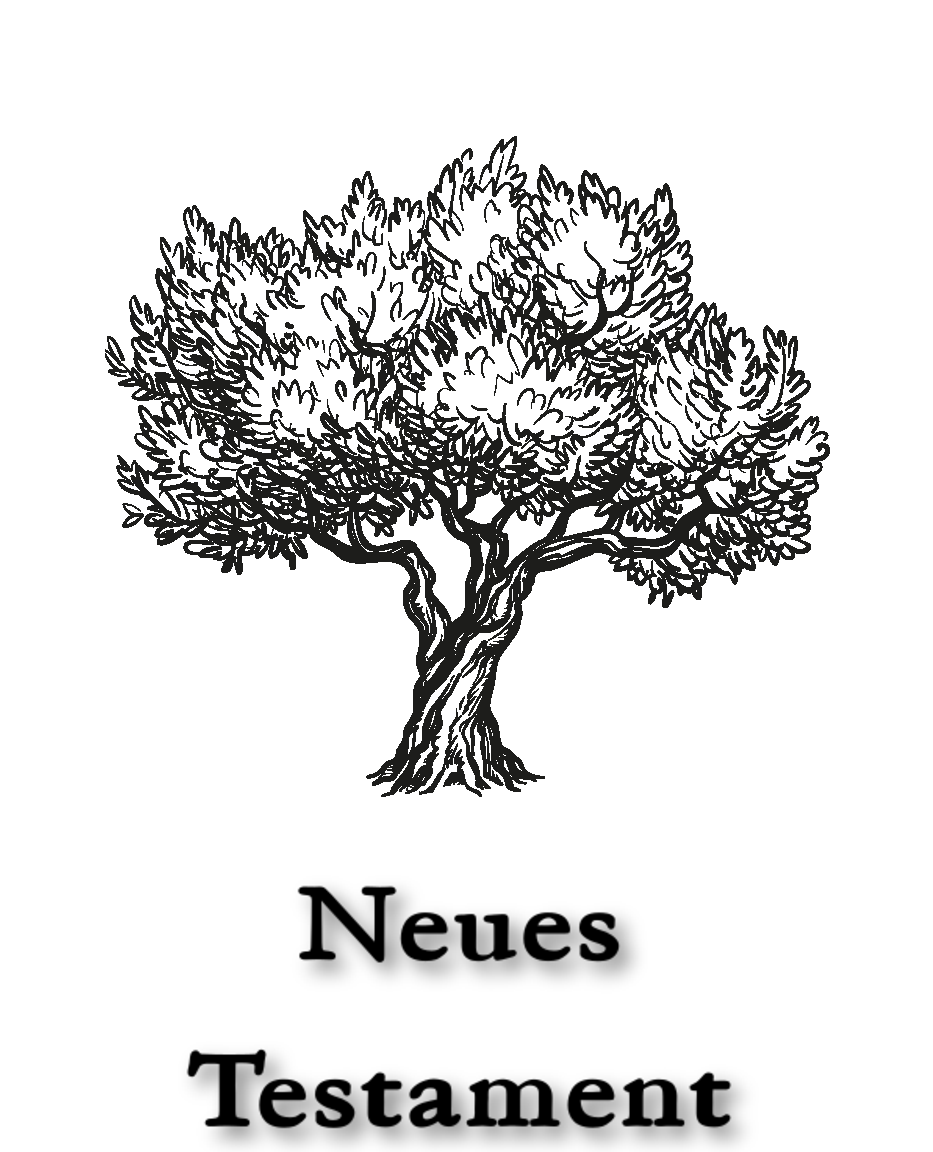
\includegraphics{NeuesTestamentTitel.pdf}
  \end{center}
\end{minipage}
\end{center}
\null\vfill
\newpage

\chapter{Offenbarung}
\begin{multicols}{2}
  \parskip=0pt \relax
  \hypertarget{section}{%
\section{1}\label{section}}

\bibverse{1} Dies ist die Offenbarung Jesu Christi, die ihm Gott gegeben
hat, seinen Knechten zu zeigen, was in der Kürze geschehen soll; und er
hat sie gedeutet und gesandt durch seinen Engel zu seinem Knecht
Johannes, \bibverse{2} der bezeugt hat das Wort Gottes und das Zeugnis
von Jesu Christo, was er gesehen hat.

\bibverse{3} Selig ist, der da liest und die da hören die Worte der
Weissagung und behalten, was darin geschrieben ist; denn die Zeit ist
nahe. \footnote{\textbf{1:3} Offb 22,10}

\bibverse{4} Johannes den sieben Gemeinden in Asien: Gnade sei mit euch
und Friede von dem, der da ist und der da war und der da kommt, und von
den sieben Geistern, die da sind vor seinem Stuhl, \footnote{\textbf{1:4}
  2Mo 3,14-15; Offb 3,1; Offb 5,6} \bibverse{5} und von Jesu Christo,
welcher ist der treue Zeuge und Erstgeborene von den Toten und der Fürst
der Könige auf Erden! Der uns geliebt hat und gewaschen von den Sünden
mit seinem Blut \footnote{\textbf{1:5} Offb 3,14; Joh 18,37; 1Tim 6,13;
  Kol 1,18} \bibverse{6} und hat uns zu Königen und Priestern gemacht
vor Gott und seinem Vater, dem sei Ehre und Gewalt von Ewigkeit zu
Ewigkeit! Amen. \footnote{\textbf{1:6} Offb 5,10; 1Petr 2,5; 1Petr 2,9;
  2Mo 19,6}

\bibverse{7} Siehe, er kommt mit den Wolken, und es werden ihn sehen
alle Augen und die ihn zerstochen haben; und werden heulen alle
Geschlechter der Erde. Ja, amen. \footnote{\textbf{1:7} Mt 24,30; Sach
  12,10; Joh 19,37}

\bibverse{8} Ich bin das A und das O, der Anfang und das Ende, spricht
Gott der Herr, der da ist und der da war und der da kommt, der
Allmächtige. \footnote{\textbf{1:8} Jes 41,4; Offb 4,8; Offb 21,6}

\bibverse{9} Ich, Johannes, der auch euer Bruder und Mitgenosse an der
Trübsal ist und am Reich und an der Geduld Jesu Christi, war auf der
Insel, die da heißt Patmos, um des Wortes Gottes willen und des
Zeugnisses Jesu Christi. \bibverse{10} Ich war im Geist an des Herrn Tag
und hörte hinter mir eine große Stimme wie einer Posaune, \bibverse{11}
die sprach: Ich bin das A und das O, der Erste und der Letzte; und was
du siehst, das schreibe in ein Buch und sende es zu den Gemeinden in
Asien: gen Ephesus und gen Smyrna und gen Pergamus und gen Thyatira und
gen Sardes und gen Philadelphia und gen Laodizea.

\bibverse{12} Und ich wandte mich um, zu sehen nach der Stimme, die mit
mir redete. Und als ich mich wandte, sah ich sieben goldene Leuchter
\bibverse{13} und mitten unter den sieben Leuchtern einen, der war eines
Menschen Sohne gleich, der war angetan mit einem langen Gewand und
begürtet um die Brust mit einem goldenen Gürtel. \footnote{\textbf{1:13}
  Offb 2,1; Dan 7,13} \bibverse{14} Sein Haupt aber und sein Haar war
weiß wie weiße Wolle, wie der Schnee, und seine Augen wie eine
Feuerflamme \footnote{\textbf{1:14} Dan 7,9; Offb 2,18; Offb 19,12}
\bibverse{15} und seine Füße gleichwie Messing, das im Ofen glüht, und
seine Stimme wie großes Wasserrauschen; \bibverse{16} und er hatte
sieben Sterne in seiner rechten Hand, und aus seinem Munde ging ein
scharfes, zweischneidiges Schwert, und sein Angesicht leuchtete wie die
helle Sonne. \bibverse{17} Und als ich ihn sah, fiel ich zu seinen Füßen
wie ein Toter; und er legte seine rechte Hand auf mich und sprach zu
mir: Fürchte dich nicht! ich bin der Erste und der Letzte \footnote{\textbf{1:17}
  Dan 8,18}

\bibverse{18} und der Lebendige; ich war tot, und siehe, ich bin
lebendig von Ewigkeit zu Ewigkeit und habe die Schlüssel der Hölle und
des Todes. \bibverse{19} Schreibe, was du gesehen hast, und was da ist,
und was geschehen soll darnach. \bibverse{20} Das Geheimnis der sieben
Sterne, die du gesehen hast in meiner rechten Hand, und die sieben
goldenen Leuchter: die sieben Sterne sind Engel der sieben Gemeinden;
und die sieben Leuchter, die du gesehen hast, sind sieben Gemeinden. \#
2 \bibverse{1} Dem Engel der Gemeinde zu Ephesus schreibe: Das sagt, der
da hält die sieben Sterne in seiner Rechten, der da wandelt mitten unter
den sieben goldenen Leuchtern:

\bibverse{2} Ich weiß deine Werke und deine Arbeit und deine Geduld und
dass du die Bösen nicht tragen kannst; und hast versucht die, die da
sagen, sie seien Apostel, und sind's nicht, und hast sie als Lügner
erfunden; \footnote{\textbf{2:2} 1Jo 4,1}

\bibverse{3} und verträgst und hast Geduld, und um meines Namens willen
arbeitest du und bist nicht müde geworden. \bibverse{4} Aber ich habe
wider dich, dass du die erste Liebe verlässest. \bibverse{5} Gedenke,
wovon du gefallen bist, und tue Buße und tue die ersten Werke. Wo aber
nicht, werde ich dir bald kommen und deinen Leuchter wegstoßen von
seiner Stätte, wenn du nicht Buße tust. \bibverse{6} Aber das hast du,
dass du die Werke der Nikolaiten hassest, welche ich auch hasse.
\footnote{\textbf{2:6} Ps 139,21} \bibverse{7} Wer Ohren hat, der höre,
was der Geist den Gemeinden sagt: Wer überwindet, dem will ich zu essen
geben vom Holz des Lebens, das im Paradies Gottes ist. \footnote{\textbf{2:7}
  Offb 22,2; 1Mo 2,9}

\bibverse{8} Und dem Engel der Gemeinde zu Smyrna schreibe: Das sagt der
Erste und der Letzte, der tot war und ist lebendig geworden: \footnote{\textbf{2:8}
  Offb 1,11; Offb 1,18}

\bibverse{9} Ich weiß deine Werke und deine Trübsal und deine Armut (du
bist aber reich) und die Lästerung von denen, die da sagen, sie seien
Juden, und sind's nicht, sondern sind des Satans Schule. \footnote{\textbf{2:9}
  Jak 2,5; Offb 3,9}

\bibverse{10} Fürchte dich vor der keinem, das du leiden wirst! Siehe,
der Teufel wird etliche von euch ins Gefängnis werfen, auf dass ihr
versucht werdet, und werdet Trübsal haben zehn Tage. Sei getreu bis an
den Tod, so will ich dir die Krone des Lebens geben. \footnote{\textbf{2:10}
  Mt 10,19; Mt 10,28; Offb 3,11; 2Tim 4,8} \bibverse{11} Wer Ohren hat,
der höre, was der Geist den Gemeinden sagt: Wer überwindet, dem soll
kein Leid geschehen von dem anderen Tode. \footnote{\textbf{2:11} Offb
  20,14}

\bibverse{12} Und dem Engel der Gemeinde zu Pergamus schreibe: Das sagt,
der da hat das scharfe, zweischneidige Schwert: \footnote{\textbf{2:12}
  Hebr 4,12}

\bibverse{13} Ich weiß, was du tust und wo du wohnst, da des Satans
Stuhl ist; und hältst an meinem Namen und hast meinen Glauben nicht
verleugnet auch in den Tagen, in welchen Antipas, mein treuer Zeuge, bei
euch getötet ist, da der Satan wohnt.

\bibverse{14} Aber ich habe ein Kleines wider dich, dass du daselbst
hast, die an der Lehre Bileams halten, welcher lehrte den Balak ein
Ärgernis aufrichten vor den Kindern Israel, zu essen Götzenopfer und
Hurerei zu treiben. \bibverse{15} Also hast du auch, die an der Lehre
der Nikolaiten halten: das hasse ich. \bibverse{16} Tue Buße; wo aber
nicht, so werde ich dir bald kommen und mit ihnen kriegen durch das
Schwert meines Mundes. \bibverse{17} Wer Ohren hat, der höre, was der
Geist den Gemeinden sagt: Wer überwindet, dem will ich zu essen geben
von dem verborgenen Manna und will ihm geben einen weißen Stein und auf
den Stein einen neuen Namen geschrieben, welchen niemand kennt, denn der
ihn empfängt. \footnote{\textbf{2:17} Ps 78,24; Jes 62,2}

\bibverse{18} Und dem Engel der Gemeinde zu Thyatira schreibe: Das sagt
der Sohn Gottes, der Augen hat wie Feuerflammen, und seine Füße sind
gleichwie Messing: \footnote{\textbf{2:18} Apg 16,14; Offb 1,14-15}

\bibverse{19} Ich weiß deine Werke und deine Liebe und deinen Dienst und
deinen Glauben und deine Geduld und dass du je länger, je mehr tust.

\bibverse{20} Aber ich habe wider dich, dass du lässest das Weib Isebel,
die da spricht, sie sei eine Prophetin, lehren und verführen meine
Knechte, Hurerei zu treiben und Götzenopfer zu essen. \footnote{\textbf{2:20}
  2Kö 9,22} \bibverse{21} Und ich habe ihr Zeit gegeben, dass sie sollte
Buße tun für ihre Hurerei; und sie tut nicht Buße. \bibverse{22} Siehe,
ich werfe sie in ein Bett, und die mit ihr die Ehe gebrochen haben, in
große Trübsal, wenn sie nicht Buße tun für ihre Werke, \bibverse{23} und
ihre Kinder will ich zu Tode schlagen. Und alle Gemeinden sollen
erkennen, dass ich es bin, der die Nieren und Herzen erforscht; und ich
werde geben einem jeglichen unter euch nach euren Werken. \bibverse{24}
Euch aber sage ich, den anderen, die zu Thyatira sind, die nicht haben
solche Lehre und die nicht erkannt haben die Tiefen des Satans (wie sie
sagen): Ich will nicht auf euch werfen eine andere Last: \bibverse{25}
doch was ihr habt, das haltet, bis dass ich komme. \footnote{\textbf{2:25}
  Offb 3,11} \bibverse{26} Und wer da überwindet und hält meine Werke
bis ans Ende, dem will ich Macht geben über die Heiden, \bibverse{27}
und er soll sie weiden mit einem eisernen Stabe, und wie eines Töpfers
Gefäße soll er sie zerschmeißen, \bibverse{28} wie ich von meinem Vater
empfangen habe; und ich will ihm geben den Morgenstern. \bibverse{29}
Wer Ohren hat, der höre, was der Geist den Gemeinden sagt! \# 3
\bibverse{1} Und dem Engel der Gemeinde zu Sardes schreibe: Das sagt,
der die sieben Geister Gottes hat und die sieben Sterne: Ich weiß deine
Werke; denn du hast den Namen, dass du lebest, und bist tot. \footnote{\textbf{3:1}
  Offb 1,4}

\bibverse{2} Werde wach und stärke das andere, das sterben will; denn
ich habe deine Werke nicht völlig erfunden vor Gott. \footnote{\textbf{3:2}
  Lk 22,32}

\bibverse{3} So gedenke nun, wie du empfangen und gehört hast, und halte
es und tue Buße. Wenn du nicht wirst wachen, werde ich über dich kommen
wie ein Dieb, und wirst nicht wissen, welche Stunde ich über dich kommen
werde. \footnote{\textbf{3:3} 1Thes 5,2} \bibverse{4} Aber du hast
etliche Namen zu Sardes, die nicht ihre Kleider besudelt haben; und sie
werden mit mir wandeln in weißen Kleidern, denn sie sind's wert.
\footnote{\textbf{3:4} Jud 1,23} \bibverse{5} Wer überwindet, der soll
mit weißen Kleidern angetan werden, und ich werde seinen Namen nicht
austilgen aus dem Buch des Lebens, und ich will seinen Namen bekennen
vor meinem Vater und vor seinen Engeln. \footnote{\textbf{3:5} Offb
  7,13; Mt 10,32; Lk 10,20} \bibverse{6} Wer Ohren hat, der höre, was
der Geist den Gemeinden sagt!

\bibverse{7} Und dem Engel der Gemeinde zu Philadelphia schreibe: Das
sagt der Heilige, der Wahrhaftige, der da hat den Schlüssel Davids, der
auftut, und niemand schließt zu, der zuschließt, und niemand tut auf:

\bibverse{8} Ich weiß deine Werke. Siehe, ich habe vor dir gegeben eine
offene Tür, und niemand kann sie zuschließen; denn du hast eine kleine
Kraft, und hast mein Wort behalten und hast meinen Namen nicht
verleugnet.

\bibverse{9} Siehe, ich werde geben aus des Satanas Schule, die da
sagen, sie seien Juden, und sind's nicht, sondern lügen; siehe, ich will
sie dazu bringen, dass sie kommen sollen und niederfallen zu deinen
Füßen und erkennen, dass ich dich geliebt habe. \footnote{\textbf{3:9}
  Offb 2,9; Jes 60,14; Jes 49,23} \bibverse{10} Dieweil du hast bewahrt
das Wort meiner Geduld, will ich auch dich bewahren vor der Stunde der
Versuchung, die kommen wird über den ganzen Weltkreis, zu versuchen, die
da wohnen auf Erden. \footnote{\textbf{3:10} Offb 14,12; Mt 6,13}
\bibverse{11} Siehe, ich komme bald; halte, was du hast, dass niemand
deine Krone nehme! \footnote{\textbf{3:11} Offb 2,10} \bibverse{12} Wer
überwindet, den will ich machen zum Pfeiler in dem Tempel meines Gottes,
und er soll nicht mehr hinausgehen; und will auf ihn schreiben den Namen
meines Gottes und den Namen des neuen Jerusalem, der Stadt meines
Gottes, die vom Himmel herniederkommt von meinem Gott, und meinen Namen,
den neuen. \footnote{\textbf{3:12} Offb 14,1; Offb 22,4; Offb 21,2}
\bibverse{13} Wer Ohren hat, der höre, was der Geist den Gemeinden sagt!

\bibverse{14} Und dem Engel der Gemeinde zu Laodizea schreibe: Das sagt,
der Amen heißt, der treue und wahrhaftige Zeuge, der Anfang der Kreatur
Gottes: \footnote{\textbf{3:14} Kol 2,1; Kol 4,13; 2Kor 1,20; Offb 1,5;
  Kol 1,15}

\bibverse{15} Ich weiß deine Werke, dass du weder kalt noch warm bist.
Ach, dass du kalt oder warm wärest!

\bibverse{16} Weil du aber lau bist und weder kalt noch warm, werde ich
dich ausspeien aus meinem Munde. \bibverse{17} Du sprichst: Ich bin
reich und habe gar satt und bedarf nichts! und weißt nicht, dass du bist
elend und jämmerlich, arm, blind und bloß. \bibverse{18} Ich rate dir,
dass du Gold von mir kaufest, das mit Feuer durchläutert ist, dass du
reich werdest, und weiße Kleider, dass du dich antust und nicht
offenbart werde die Schande deiner Blöße; und salbe deine Augen mit
Augensalbe, dass du sehen mögest. \footnote{\textbf{3:18} Jes 55,1}
\bibverse{19} Welche ich liebhabe, die strafe und züchtige ich. So sei
nun fleißig und tue Buße! \footnote{\textbf{3:19} Spr 3,12; Hebr 12,6;
  1Kor 11,32} \bibverse{20} Siehe, ich stehe vor der Tür und klopfe an.
Wenn jemand meine Stimme hören wird und die Tür auftun, zu dem werde ich
eingehen und das Abendmahl mit ihm halten und er mit mir. \footnote{\textbf{3:20}
  Joh 14,23} \bibverse{21} Wer überwindet, dem will ich geben, mit mir
auf meinem Stuhl zu sitzen, wie ich überwunden habe und mich gesetzt mit
meinem Vater auf seinen Stuhl. \footnote{\textbf{3:21} Mt 19,28}
\bibverse{22} Wer Ohren hat, der höre, was der Geist den Gemeinden sagt!
\# 4 \bibverse{1} Darnach sah ich, und siehe, eine Tür war aufgetan im
Himmel; und die erste Stimme, die ich gehört hatte mit mir reden wie
eine Posaune, die sprach: Steig her, ich will dir zeigen, was nach
diesem geschehen soll. \footnote{\textbf{4:1} Offb 1,10}

\bibverse{2} Und alsobald war ich im Geist. Und siehe, ein Stuhl war
gesetzt im Himmel, und auf dem Stuhl saß einer; \footnote{\textbf{4:2}
  Jes 6,1; Ps 47,9} \bibverse{3} und der da saß, war gleich anzusehen
wie der Stein Jaspis und Sarder; und ein Regenbogen war um den Stuhl,
gleich anzusehen wie ein Smaragd. \footnote{\textbf{4:3} Hes 1,26-28}
\bibverse{4} Und um den Stuhl waren vierundzwanzig Stühle, und auf den
Stühlen saßen vierundzwanzig Älteste, mit weißen Kleidern angetan, und
hatten auf ihren Häuptern goldene Kronen. \bibverse{5} Und von dem Stuhl
gingen aus Blitze, Donner und Stimmen; und sieben Fackeln mit Feuer
brannten vor dem Stuhl, welches sind die sieben Geister Gottes.
\bibverse{6} Und vor dem Stuhl war ein gläsernes Meer gleich dem
Kristall, und mitten am Stuhl und um den Stuhl vier Tiere, voll Augen
vorn und hinten. \footnote{\textbf{4:6} Hes 1,5; Hes 1,10; Hes 1,22; Hes
  10,14} \bibverse{7} Und das erste Tier war gleich einem Löwen, und das
andere Tier war gleich einem Kalbe, das dritte hatte ein Antlitz wie ein
Mensch, und das vierte Tier war gleich einem fliegenden Adler.
\bibverse{8} Und ein jegliches der vier Tiere hatte sechs Flügel, und
sie waren außenherum und inwendig voll Augen und hatten keine Ruhe Tag
und Nacht und sprachen: Heilig, heilig, heilig ist Gott der Herr, der
Allmächtige, der da war und der da ist und der da kommt!

\bibverse{9} Und da die Tiere gaben Preis und Ehre und Dank dem, der da
auf dem Stuhl saß, der da lebt von Ewigkeit zu Ewigkeit, \bibverse{10}
fielen die vierundzwanzig Ältesten nieder vor dem, der auf dem Stuhl
saß, und beteten an den, der da lebt von Ewigkeit zu Ewigkeit, und
warfen ihre Kronen vor den Stuhl und sprachen: \bibverse{11} Herr, du
bist würdig, zu nehmen Preis und Ehre und Kraft; denn du hast alle Dinge
geschaffen, und durch deinen Willen haben sie das Wesen und sind
geschaffen. \# 5 \bibverse{1} Und ich sah in der rechten Hand des, der
auf dem Stuhl saß, ein Buch, beschrieben inwendig und auswendig,
versiegelt mit sieben Siegeln. \footnote{\textbf{5:1} Offb 4,2; Hes
  2,9-10} \bibverse{2} Und ich sah einen starken Engel, der rief aus mit
großer Stimme: Wer ist würdig, das Buch aufzutun und seine Siegel zu
brechen? \bibverse{3} Und niemand im Himmel noch auf Erden noch unter
der Erde konnte das Buch auftun und hineinsehen. \bibverse{4} Und ich
weinte sehr, dass niemand würdig erfunden ward, das Buch aufzutun und zu
lesen noch hineinzusehen. \bibverse{5} Und einer von den Ältesten
spricht zu mir: Weine nicht! Siehe, es hat überwunden der Löwe, der da
ist vom Geschlecht Juda, die Wurzel Davids, aufzutun das Buch und zu
brechen seine sieben Siegel.

\bibverse{6} Und ich sah, und siehe, mitten zwischen dem Stuhl und den
vier Tieren und zwischen den Ältesten stand ein Lamm, wie wenn es
erwürgt wäre, und hatte sieben Hörner und sieben Augen, das sind die
sieben Geister Gottes, gesandt in alle Lande. \footnote{\textbf{5:6} Jes
  53,7; Joh 1,29} \bibverse{7} Und es kam und nahm das Buch aus der Hand
des, der auf dem Stuhl saß. \bibverse{8} Und da es das Buch nahm, da
fielen die vier Tiere und die vierundzwanzig Ältesten nieder vor dem
Lamm und hatten ein jeglicher Harfen und goldene Schalen voll Räuchwerk,
das sind die Gebete der Heiligen, \bibverse{9} und sangen ein neues Lied
und sprachen: Du bist würdig, zu nehmen das Buch und aufzutun seine
Siegel; denn du bist erwürget und hast uns Gott erkauft mit deinem Blut
aus allerlei Geschlecht und Zunge und Volk und Heiden \bibverse{10} und
hast uns unserem Gott zu Königen und Priestern gemacht, und wir werden
Könige sein auf Erden. \footnote{\textbf{5:10} Offb 1,6; 2Mo 19,6}

\bibverse{11} Und ich sah und hörte eine Stimme vieler Engel um den
Stuhl und um die Tiere und um die Ältesten her; und ihre Zahl war
vieltausendmal tausend; \footnote{\textbf{5:11} Hebr 12,22}
\bibverse{12} und sie sprachen mit großer Stimme: Das Lamm, das erwürget
ist, ist würdig, zu nehmen Kraft und Reichtum und Weisheit und Stärke
und Ehre und Preis und Lob. \footnote{\textbf{5:12} 1Chr 29,11; Phil
  2,9-10}

\bibverse{13} Und alle Kreatur, die im Himmel ist und auf Erden und
unter der Erde und im Meer, und alles, was darinnen ist, hörte ich
sagen: Dem, der auf dem Stuhl sitzt, und dem Lamm sei Lob und Ehre und
Preis und Gewalt von Ewigkeit zu Ewigkeit!

\bibverse{14} Und die vier Tiere sprachen: Amen! Und die vierundzwanzig
Ältesten fielen nieder und beteten an den, der da lebt von Ewigkeit zu
Ewigkeit. \# 6 \bibverse{1} Und ich sah, dass das Lamm der Siegel eines
auftat; und ich hörte der vier Tiere eines sagen wie mit einer
Donnerstimme: Komm! \bibverse{2} Und ich sah, und siehe, ein weißes
Pferd. Und der darauf saß, hatte einen Bogen; und ihm ward gegeben eine
Krone, und er zog aus sieghaft, und dass er siegte.

\bibverse{3} Und da es das andere Siegel auftat, hörte ich das andere
Tier sagen: Komm! \bibverse{4} Und es ging heraus ein anderes Pferd, das
war rot. Und dem, der darauf saß, ward gegeben, den Frieden zu nehmen
von der Erde und dass sie sich untereinander erwürgten; und ihm ward ein
großes Schwert gegeben.

\bibverse{5} Und da es das dritte Siegel auftat, hörte ich das dritte
Tier sagen: Komm! Und ich sah, und siehe, ein schwarzes Pferd. Und der
darauf saß, hatte eine Waage in seiner Hand. \bibverse{6} Und ich hörte
eine Stimme unter den vier Tieren sagen: Ein Maß Weizen um einen
Groschen und drei Maß Gerste um einen Groschen; und dem Öl und Wein tu
kein Leid! \footnote{\textbf{6:6} 2Kö 6,25; 2Kö 7,1}

\bibverse{7} Und da es das vierte Siegel auftat, hörte ich die Stimme
des vierten Tieres sagen: Komm! \bibverse{8} Und ich sah, und siehe, ein
fahles Pferd. Und der darauf saß, des Name hieß Tod, und die Hölle
folgte ihm nach. Und ihnen ward Macht gegeben, zu töten den vierten Teil
auf der Erde mit dem Schwert und Hunger und mit dem Tod und durch die
Tiere auf Erden.

\bibverse{9} Und da es das fünfte Siegel auftat, sah ich unter dem Altar
die Seelen derer, die erwürgt waren um des Wortes Gottes willen und um
des Zeugnisses willen, das sie hatten. \bibverse{10} Und sie schrien mit
großer Stimme und sprachen: Herr, du Heiliger und Wahrhaftiger, wie
lange richtest du nicht und rächest unser Blut an denen, die auf der
Erde wohnen? \bibverse{11} Und ihnen wurde gegeben einem jeglichen ein
weißes Kleid, und ward zu ihnen gesagt, dass sie ruhten noch eine kleine
Zeit, bis dass vollends dazukämen ihre Mitknechte und Brüder, die auch
sollten noch getötet werden gleich wie sie.

\bibverse{12} Und ich sah, dass es das sechste Siegel auftat, und siehe,
da ward ein großes Erdbeben, und die Sonne ward schwarz wie ein härener
Sack, und der Mond ward wie Blut; \footnote{\textbf{6:12} Jes 24,21-23;
  Joe 3,3-4; Mt 24,29} \bibverse{13} und die Sterne des Himmels fielen
auf die Erde, gleichwie ein Feigenbaum seine Feigen abwirft, wenn er von
großem Wind bewegt wird. \footnote{\textbf{6:13} Jes 34,4} \bibverse{14}
Und der Himmel entwich wie ein zusammengerolltes Buch; und alle Berge
und Inseln wurden bewegt aus ihren Örtern. \bibverse{15} Und die Könige
auf Erden und die Großen und die Reichen und die Hauptleute und die
Gewaltigen und alle Knechte und alle Freien verbargen sich in den
Klüften und Felsen an den Bergen \footnote{\textbf{6:15} Jes 2,10; Jes
  2,19} \bibverse{16} und sprachen zu den Bergen und Felsen: Fallet über
uns und verberget uns vor dem Angesichte des, der auf dem Stuhl sitzt,
und vor dem Zorn des Lammes! \footnote{\textbf{6:16} Lk 23,30}
\bibverse{17} Denn es ist gekommen der große Tag seines Zorns, und wer
kann bestehen? \footnote{\textbf{6:17} Am 5,18; Röm 2,5; Mal 3,2}

\hypertarget{section-1}{%
\section{7}\label{section-1}}

\bibverse{1} Und darnach sah ich vier Engel stehen auf den vier Ecken
der Erde, die hielten die vier Winde der Erde, auf dass kein Wind über
die Erde bliese noch über das Meer noch über irgend einen Baum.
\footnote{\textbf{7:1} Dan 7,2} \bibverse{2} Und ich sah einen anderen
Engel aufsteigen von der Sonne Aufgang, der hatte das Siegel des
lebendigen Gottes und schrie mit großer Stimme zu den vier Engeln,
welchen gegeben war zu beschädigen die Erde und das Meer; \bibverse{3}
und er sprach: Beschädiget die Erde nicht noch das Meer noch die Bäume,
bis dass wir versiegeln die Knechte unseres Gottes an ihren Stirnen!
\footnote{\textbf{7:3} Offb 9,4; Hes 9,4; Hes 9,6} \bibverse{4} Und ich
hörte die Zahl derer, die versiegelt wurden:
hundertvierundvierzigtausend, die versiegelt waren von allen
Geschlechtern der Kinder Israel: \footnote{\textbf{7:4} Offb 14,1; Offb
  14,3} \bibverse{5} von dem Geschlechte Juda zwölftausend versiegelt;
von dem Geschlechte Ruben zwölftausend versiegelt; von dem Geschlechte
Gad zwölftausend versiegelt; \bibverse{6} von dem Geschlechte Asser
zwölftausend versiegelt; von dem Geschlechte Naphthali zwölftausend
versiegelt; von dem Geschlechte Manasse zwölftausend versiegelt;
\bibverse{7} von dem Geschlechte Simeon zwölftausend versiegelt; von dem
Geschlechte Levi zwölftausend versiegelt; von dem Geschlechte Isaschar
zwölftausend versiegelt; \bibverse{8} von dem Geschlechte Sebulon
zwölftausend versiegelt; von dem Geschlechte Joseph zwölftausend
versiegelt; von dem Geschlechte Benjamin zwölftausend versiegelt.

\bibverse{9} Darnach sah ich, und siehe, eine große Schar, welche
niemand zählen konnte, aus allen Heiden und Völkern und Sprachen, vor
dem Stuhl stehend und vor dem Lamm, angetan mit weißen Kleidern und
Palmen in ihren Händen, \bibverse{10} schrien mit großer Stimme und
sprachen: Heil sei dem, der auf dem Stuhl sitzt, unserem Gott, und dem
Lamm!

\bibverse{11} Und alle Engel standen um den Stuhl und um die Ältesten
und um die vier Tiere und fielen vor dem Stuhl auf ihr Angesicht und
beteten Gott an \bibverse{12} und sprachen: Amen, Lob und Ehre und
Weisheit und Dank und Preis und Kraft und Stärke sei unserem Gott von
Ewigkeit zu Ewigkeit! Amen.

\bibverse{13} Und es antwortete der Ältesten einer und sprach zu mir:
Wer sind diese, mit den weißen Kleidern angetan, und woher sind sie
gekommen?

\bibverse{14} Und ich sprach zu ihm: Herr, du weißt es. Und er sprach zu
mir: Diese sind's, die gekommen sind aus großer Trübsal und haben ihre
Kleider gewaschen und haben ihre Kleider hell gemacht im Blut des
Lammes. \footnote{\textbf{7:14} Offb 12,11; Mt 24,21}

\bibverse{15} Darum sind sie vor dem Stuhl Gottes und dienen ihm Tag und
Nacht in seinem Tempel; und der auf dem Stuhl sitzt, wird über ihnen
wohnen. \bibverse{16} Sie wird nicht mehr hungern noch dürsten; es wird
auch nicht auf sie fallen die Sonne oder irgendeine Hitze; \bibverse{17}
denn das Lamm mitten im Stuhl wird sie weiden und leiten zu den
lebendigen Wasserbrunnen, und Gott wird abwischen alle Tränen von ihren
Augen. \footnote{\textbf{7:17} Ps 23,2; Offb 21,4; Jes 25,8}

\hypertarget{section-2}{%
\section{8}\label{section-2}}

\bibverse{1} Und da es das siebente Siegel auftat, ward eine Stille in
dem Himmel bei einer halben Stunde. \footnote{\textbf{8:1} Sach 2,17;
  Hab 2,20} \bibverse{2} Und ich sah die sieben Engel, die da stehen vor
Gott, und ihnen wurden sieben Posaunen gegeben. \footnote{\textbf{8:2}
  Mt 24,31}

\bibverse{3} Und ein anderer Engel kam und trat an den Altar und hatte
ein goldenes Räuchfass; und ihm ward viel Räuchwerk gegeben, dass er es
gäbe zum Gebet aller Heiligen auf den goldenen Altar vor dem Stuhl.
\bibverse{4} Und der Rauch des Räuchwerks vom Gebet der Heiligen ging
auf von der Hand des Engels vor Gott. \bibverse{5} Und der Engel nahm
das Räuchfass und füllte es mit Feuer vom Altar und schüttete es auf die
Erde. Und da geschahen Stimmen und Donner und Blitze und Erdbeben.
\footnote{\textbf{8:5} Hes 10,2}

\bibverse{6} Und die sieben Engel mit den sieben Posaunen hatten sich
gerüstet, zu posaunen.

\bibverse{7} Und der erste Engel posaunte: und es ward ein Hagel und
Feuer, mit Blut gemengt, und fiel auf die Erde; und der dritte Teil der
Bäume verbrannte, und alles grüne Gras verbrannte.

\bibverse{8} Und der andere Engel posaunte: und es fuhr wie ein großer
Berg mit Feuer brennend ins Meer; und der dritte Teil des Meeres ward
Blut, \footnote{\textbf{8:8} 2Mo 7,20-21} \bibverse{9} und der dritte
Teil der lebendigen Kreaturen im Meer starben, und der dritte Teil der
Schiffe wurden verderbt.

\bibverse{10} Und der dritte Engel posaunte: und es fiel ein großer
Stern vom Himmel, der brannte wie eine Fackel und fiel auf den dritten
Teil der Wasserströme und über die Wasserbrunnen. \bibverse{11} Und der
Name des Sterns heißt Wermut. Und der dritte Teil der Wasser ward
Wermut; und viele Menschen starben von den Wassern, weil sie waren so
bitter geworden.

\bibverse{12} Und der vierte Engel posaunte: und es ward geschlagen der
dritte Teil der Sonne und der dritte Teil des Mondes und der dritte Teil
der Sterne, dass ihr dritter Teil verfinstert ward und der Tag den
dritten Teil nicht schien und die Nacht desgleichen. \footnote{\textbf{8:12}
  Offb 6,12; 2Mo 10,21} \bibverse{13} Und ich sah und hörte einen Engel
fliegen mitten durch den Himmel und sagen mit großer Stimme: Weh, weh,
weh denen, die auf Erden wohnen, vor den anderen Stimmen der Posaune der
drei Engel, die noch posaunen sollen! \# 9 \bibverse{1} Und der fünfte
Engel posaunte: und ich sah einen Stern, gefallen vom Himmel auf die
Erde; und ihm ward der Schlüssel zum Brunnen des Abgrunds gegeben.
\bibverse{2} Und er tat den Brunnen des Abgrunds auf; und es ging auf
ein Rauch aus dem Brunnen wie ein Rauch eines großen Ofens, und es ward
verfinstert die Sonne und die Luft von dem Rauch des Brunnens.
\bibverse{3} Und aus dem Rauch kamen Heuschrecken auf die Erde; und
ihnen ward Macht gegeben, wie die Skorpione auf Erden Macht haben.
\bibverse{4} Und es ward ihnen gesagt, dass sie nicht beschädigten das
Gras auf Erden noch ein Grünes noch einen Baum, sondern allein die
Menschen, die nicht haben das Siegel Gottes an ihren Stirnen.
\footnote{\textbf{9:4} Offb 7,3} \bibverse{5} Und es ward ihnen gegeben,
dass sie sie nicht töteten, sondern sie quälten fünf Monate lang; und
ihre Qual war wie eine Qual vom Skorpion, wenn er einen Menschen
schlägt. \bibverse{6} Und in den Tagen werden die Menschen den Tod
suchen, und nicht finden; werden begehren zu sterben, und der Tod wird
vor ihnen fliehen.

\bibverse{7} Und die Heuschrecken sind gleich den Rossen, die zum Kriege
bereitet sind; und auf ihrem Haupt wie Kronen, dem Golde gleich, und ihr
Antlitz gleich der Menschen Antlitz; \bibverse{8} und hatten Haare wie
Weiberhaare, und ihre Zähne waren wie die der Löwen; \bibverse{9} und
hatten Panzer wie eiserne Panzer, und das Rasseln ihrer Flügel wie das
Rasseln an den Wagen vieler Rosse, die in den Krieg laufen;
\bibverse{10} und hatten Schwänze gleich den Skorpionen, und es waren
Stacheln an ihren Schwänzen; und ihre Macht war, zu beschädigen die
Menschen fünf Monate lang. \bibverse{11} Und hatten über sich einen
König, den Engel des Abgrunds, des Name heißt auf hebräisch Abaddon, und
auf griechisch hat er den Namen Apollyon.

\bibverse{12} Ein Wehe ist dahin; siehe, es kommen noch zwei Wehe nach
dem.

\bibverse{13} Und der sechste Engel posaunte: und ich hörte eine Stimme
aus den vier Ecken des goldenen Altars vor Gott, \footnote{\textbf{9:13}
  Offb 8,3; 2Mo 27,2; 2Mo 30,1-3} \bibverse{14} die sprach zu dem
sechsten Engel, der die Posaune hatte: Löse die vier Engel, die gebunden
sind an dem großen Wasserstrom Euphrat. \footnote{\textbf{9:14} Offb
  16,12}

\bibverse{15} Und es wurden die vier Engel los, die bereit waren auf die
Stunde und auf den Tag und auf den Monat und auf das Jahr, dass sie
töteten den dritten Teil der Menschen. \footnote{\textbf{9:15} Offb 8,-1}
\bibverse{16} Und die Zahl des reisigen Volkes war vieltausendmal
tausend; und ich hörte ihre Zahl. \bibverse{17} Und also sah ich die
Rosse im Gesicht und die darauf saßen, dass sie hatten feurige und
bläuliche und schwefelige Panzer; und die Häupter der Rosse waren wie
die Häupter der Löwen, und aus ihrem Munde ging Feuer und Rauch und
Schwefel. \bibverse{18} Von diesen drei Plagen ward getötet der dritte
Teil der Menschen, von dem Feuer und Rauch und Schwefel, der aus ihrem
Munde ging. \bibverse{19} Denn ihre Macht war in ihrem Munde; und ihre
Schwänze waren den Schlangen gleich und hatten Häupter, und mit
denselben taten sie Schaden.

\bibverse{20} Und die übrigen Leute, die nicht getötet wurden von diesen
Plagen, taten nicht Buße für die Werke ihrer Hände, dass sie nicht
anbeteten die Teufel und goldenen, silbernen, ehernen, steinernen und
hölzernen Götzen, welche weder sehen noch hören noch wandeln können;
\bibverse{21} und taten auch nicht Buße für ihre Morde, Zauberei,
Hurerei und Dieberei. \# 10 \bibverse{1} Und ich sah einen anderen
starken Engel vom Himmel herabkommen; der war mit einer Wolke bekleidet,
und ein Regenbogen auf seinem Haupt und sein Antlitz wie die Sonne und
Füße wie Feuersäulen, \bibverse{2} und er hatte in seiner Hand ein
Büchlein aufgetan. Und er setzte seinen rechten Fuß auf das Meer und den
linken auf die Erde; \bibverse{3} und er schrie mit großer Stimme, wie
ein Löwe brüllt. Und da er schrie, redeten sieben Donner ihre Stimmen.
\footnote{\textbf{10:3} Hos 11,10; Am 1,2; Jer 25,30} \bibverse{4} Und
da die sieben Donner ihre Stimmen geredet hatten, wollte ich sie
schreiben. Da hörte ich eine Stimme vom Himmel sagen zu mir: Versiegle,
was die sieben Donner geredet haben; schreibe es nicht! \footnote{\textbf{10:4}
  Dan 12,4; Dan 12,9; Ps 29,-1}

\bibverse{5} Und der Engel, den ich sah stehen auf dem Meer und der
Erde, hob seine Hand gen Himmel \bibverse{6} und schwur bei dem
Lebendigen von Ewigkeit zu Ewigkeit, der den Himmel geschaffen hat und
was darin ist, und die Erde und was darin ist, und das Meer und was
darin ist, dass hinfort keine Zeit mehr sein soll; \footnote{\textbf{10:6}
  Dan 12,7} \bibverse{7} sondern in den Tagen der Stimme des siebenten
Engels, wenn er posaunen wird, soll vollendet werden das Geheimnis
Gottes, wie er hat verkündigt seinen Knechten, den Propheten.
\footnote{\textbf{10:7} Offb 11,15; Apg 3,21}

\bibverse{8} Und ich hörte eine Stimme vom Himmel abermals mit mir reden
und sagen: Gehe hin, nimm das offene Büchlein von der Hand des Engels,
der auf dem Meer und der Erde steht!

\bibverse{9} Und ich ging hin zu dem Engel und sprach zu ihm: Gib mir
das Büchlein! Und er sprach zu mir: Nimm hin und verschling es! und es
wird dich im Bauch grimmen; aber in deinem Munde wird's süß sein wie
Honig. \footnote{\textbf{10:9} Hes 3,1-3}

\bibverse{10} Und ich nahm das Büchlein von der Hand des Engels und
verschlang es, und es war süß in meinem Munde wie Honig; und da ich's
gegessen hatte, grimmte mich's im Bauch.

\bibverse{11} Und er sprach zu mir: Du musst abermals weissagen von
Völkern und Heiden und Sprachen und vielen Königen. \# 11 \bibverse{1}
Und es ward mir ein Rohr gegeben, einem Stecken gleich, und er sprach:
Stehe auf und miss den Tempel Gottes und den Altar und die darin
anbeten. \footnote{\textbf{11:1} Hes 40,3; Hes 42,20; Sach 2,5-6}
\bibverse{2} Aber den Vorhof außerhalb des Tempels wirf hinaus und miss
ihn nicht; denn er ist den Heiden gegeben, und die heilige Stadt werden
sie zertreten zweiundvierzig Monate. \footnote{\textbf{11:2} Lk 21,24}
\bibverse{3} Und ich will meinen zwei Zeugen geben, dass sie sollen
weissagen tausendzweihundertsechzig Tage, angetan mit Säcken.
\footnote{\textbf{11:3} Offb 12,6}

\bibverse{4} Diese sind die zwei Ölbäume und die Fackeln, stehend vor
dem Herrn der Erde. \footnote{\textbf{11:4} Sach 4,3; Sach 4,11-14}
\bibverse{5} Und wenn jemand sie will schädigen, so geht Feuer aus ihrem
Munde und verzehrt ihre Feinde; und wenn jemand sie will schädigen, der
muss also getötet werden. \bibverse{6} Diese haben Macht, den Himmel zu
verschließen, dass es nicht regne in den Tagen ihrer Weissagung, und
haben Macht über das Wasser, es zu wandeln in Blut, und zu schlagen die
Erde mit allerlei Plage, so oft sie wollen. \footnote{\textbf{11:6} 1Kö
  17,1; 2Mo 7,19-20}

\bibverse{7} Und wenn sie ihr Zeugnis geendet haben, so wird das Tier,
das aus dem Abgrund aufsteigt, mit ihnen einen Streit halten und wird
sie überwinden und wird sie töten. \footnote{\textbf{11:7} Offb 13,1;
  Offb 13,7} \bibverse{8} Und ihre Leichname werden liegen auf der Gasse
der großen Stadt, die da heißt geistlich „Sodom und Ägypten``, da auch
ihr Herr gekreuzigt ist. \bibverse{9} Und es werden etliche von den
Völkern und Geschlechter und Sprachen ihre Leichname sehen drei Tage und
einen halben und werden ihre Leichname nicht lassen in Gräber legen.
\bibverse{10} Und die auf Erden wohnen, werden sich freuen über sie und
wohlleben und Geschenke untereinander senden; denn diese zwei Propheten
quälten die auf Erden wohnten.

\bibverse{11} Und nach drei Tagen und einem halben fuhr in sie der Geist
des Lebens von Gott, und sie traten auf ihre Füße; und eine große Furcht
fiel über die, die sie sahen. \bibverse{12} Und sie hörten eine große
Stimme von Himmel zu ihnen sagen: Steiget herauf! Und sie stiegen auf in
den Himmel in einer Wolke, und es sahen sie ihre Feinde. \bibverse{13}
Und zu derselben Stunde ward ein großes Erdbeben, und der zehnte Teil
der Stadt fiel; und wurden getötet in dem Erdbeben siebentausend Namen
der Menschen, und die anderen erschraken und gaben Ehre dem Gott des
Himmels.

\bibverse{14} Das andere Wehe ist dahin; siehe, das dritte Wehe kommt
schnell. \footnote{\textbf{11:14} Offb 9,12}

\bibverse{15} Und der siebente Engel posaunte: und es wurden große
Stimmen im Himmel, die sprachen: Es sind die Reiche der Welt unseres
Herrn und seines Christus geworden, und er wird regieren von Ewigkeit zu
Ewigkeit.

\bibverse{16} Und die vierundzwanzig Ältesten, die vor Gott auf ihren
Stühlen saßen, fielen auf ihr Angesicht und beteten Gott an
\bibverse{17} und sprachen: Wir danken dir, Herr, allmächtiger Gott, der
du bist und warest, dass du hast angenommen deine große Kraft und
herrschest; \bibverse{18} und die Heiden sind zornig geworden, und es
ist gekommen dein Zorn und die Zeit der Toten, zu richten und zu geben
den Lohn deinen Knechten, den Propheten, und den Heiligen und denen, die
deinen Namen fürchten, den Kleinen und Großen, und zu verderben, die die
Erde verderbt haben. \footnote{\textbf{11:18} Ps 2,1}

\bibverse{19} Und der Tempel Gottes ward aufgetan im Himmel, und die
Lade seines Bundes ward in seinem Tempel gesehen; und es geschahen
Blitze und Stimmen und Donner und Erdbeben und ein großer Hagel.
\footnote{\textbf{11:19} Offb 15,5}

\hypertarget{section-3}{%
\section{12}\label{section-3}}

\bibverse{1} Und es erschien ein großes Zeichen im Himmel: ein Weib, mit
der Sonne bekleidet, und der Mond unter ihren Füßen und auf ihrem Haupt
eine Krone von zwölf Sternen. \bibverse{2} Und sie war schwanger und
schrie in Kindesnöten und hatte große Qual zur Geburt.

\bibverse{3} Und es erschien ein anderes Zeichen im Himmel, und siehe,
ein großer, roter Drache, der hatte sieben Häupter und zehn Hörner und
auf seinen Häuptern sieben Kronen; \bibverse{4} und sein Schwanz zog den
dritten Teil der Sterne des Himmels hinweg und warf sie auf die Erde.
Und der Drache trat vor das Weib, die gebären sollte, auf dass, wenn sie
geboren hätte, er ihr Kind fräße. \footnote{\textbf{12:4} Dan 8,10}
\bibverse{5} Und sie gebar einen Sohn, ein Knäblein, der alle Heiden
sollte weiden mit eisernem Stabe. Und ihr Kind ward entrückt zu Gott und
seinem Stuhl. \footnote{\textbf{12:5} Ps 2,9} \bibverse{6} Und das Weib
entfloh in die Wüste, wo sie einen Ort hat, bereitet von Gott, dass sie
daselbst ernährt würde tausendzweihundertsechzig Tage. \footnote{\textbf{12:6}
  Offb 19,2; 1Mo 3,1; Lk 10,18}

\bibverse{7} Und es erhob sich ein Streit im Himmel: Michael und seine
Engel stritten mit dem Drachen; und der Drache stritt und seine Engel,
\bibverse{8} und siegten nicht, auch ward ihre Stätte nicht mehr
gefunden im Himmel. \bibverse{9} Und es ward ausgeworfen der große
Drache, die alte Schlange, die da heißt der Teufel und Satanas, der die
ganze Welt verführt, und ward geworfen auf die Erde, und seine Engel
wurden auch dahin geworfen.

\bibverse{10} Und ich hörte eine große Stimme, die sprach im Himmel: Nun
ist das Heil und die Kraft und das Reich unseres Gottes geworden und die
Macht seines Christus, weil der Verkläger unserer Brüder verworfen ist,
der sie verklagte Tag und Nacht vor Gott. \bibverse{11} Und sie haben
ihn überwunden durch des Lammes Blut und durch das Wort ihres Zeugnisses
und haben ihr Leben nicht geliebt bis an den Tod. \footnote{\textbf{12:11}
  Offb 6,9; Offb 7,14} \bibverse{12} Darum freuet euch, ihr Himmel und
die darin wohnen! Weh denen, die auf Erden wohnen und auf dem Meer! denn
der Teufel kommt zu euch hinab und hat einen großen Zorn und weiß, dass
er wenig Zeit hat.

\bibverse{13} Und da der Drache sah, dass er verworfen war auf die Erde,
verfolgte er das Weib, die das Knäblein geboren hatte. \bibverse{14} Und
es wurden dem Weibe zwei Flügel gegeben wie eines großen Adlers, dass
sie in die Wüste flöge an ihren Ort, da sie ernährt würde eine Zeit und
zwei Zeiten und eine halbe Zeit vor dem Angesicht der Schlange.
\bibverse{15} Und die Schlange schoss nach dem Weibe aus ihrem Munde ein
Wasser wie einen Strom, dass er sie ersäufte. \bibverse{16} Aber die
Erde half dem Weibe und tat ihren Mund auf und verschlang den Strom, den
der Drache aus seinem Munde schoss. \bibverse{17} Und der Drache ward
zornig über das Weib und ging hin zu streiten mit den Übrigen von ihrem
Samen, die da Gottes Gebote halten und haben das Zeugnis Jesu Christi.
\bibverse{18} Und ich trat an den Sand des Meeres \# 13 \bibverse{1} und
sah ein Tier aus dem Meer steigen, das hatte sieben Häupter und zehn
Hörner und auf seinen Hörnern zehn Kronen und auf seinen Häuptern Namen
der Lästerung. \bibverse{2} Und das Tier, dass ich sah, war gleich einem
Parder und seine Füße wie Bärenfüße und sein Mund wie eines Löwen Mund.
Und der Drache gab ihm seine Kraft und seinen Stuhl und große Macht.
\bibverse{3} Und ich sah seiner Häupter eines, als wäre es tödlich wund;
und seine tödliche Wunde ward heil. Und der ganze Erdboden verwunderte
sich des Tieres, \bibverse{4} und sie beteten den Drachen an, der dem
Tier die Macht gab, und beteten das Tier an und sprachen: Wer ist dem
Tier gleich, und wer kann mit ihm kriegen?

\bibverse{5} Und es ward ihm gegeben ein Mund, zu reden große Dinge und
Lästerungen, und ward ihm gegeben, dass es mit ihm währte zweiundvierzig
Monate lang. \footnote{\textbf{13:5} Offb 11,2} \bibverse{6} Und es tat
seinen Mund auf zur Lästerung gegen Gott, zu lästern seinen Namen und
seine Hütte und die im Himmel wohnen. \bibverse{7} Und ihm ward gegeben,
zu streiten mit den Heiligen und sie zu überwinden; und ihm ward gegeben
Macht über alle Geschlechter und Sprachen und Heiden. \bibverse{8} Und
alle, die auf Erden wohnen, beten es an, deren Namen nicht geschrieben
sind in dem Lebensbuch des Lammes, das erwürgt ist, von Anfang der Welt.
\bibverse{9} Hat jemand Ohren, der höre! \bibverse{10} Wenn jemand in
das Gefängnis führt, der wird in das Gefängnis gehen; wenn jemand mit
dem Schwert tötet, der muss mit dem Schwert getötet werden. Hier ist
Geduld und Glaube der Heiligen. \footnote{\textbf{13:10} Mt 26,52; Offb
  14,12}

\bibverse{11} Und ich sah ein anderes Tier aufsteigen aus der Erde; das
hatte zwei Hörner gleichwie ein Lamm und redete wie ein Drache.
\bibverse{12} Und es übt alle Macht des ersten Tieres vor ihm; und es
macht, dass die Erde und die darauf wohnen anbeten das erste Tier,
dessen tödliche Wunde heil geworden war; \bibverse{13} und tut große
Zeichen, dass es auch macht Feuer vom Himmel fallen vor den Menschen;
\bibverse{14} und verführt, die auf Erden wohnen, um der Zeichen willen,
die ihm gegeben sind zu tun vor dem Tier; und sagt denen, die auf Erden
wohnen, dass sie ein Bild machen sollen dem Tier, das die Wunde vom
Schwert hatte und lebendig geworden war. \bibverse{15} Und es ward ihm
gegeben, dass es dem Bilde des Tieres den Geist gab, dass des Tieres
Bild redete und machte, dass alle, welche nicht des Tieres Bild
anbeteten, getötet würden. \bibverse{16} Und es macht, dass die Kleinen
und Großen, die Reichen und Armen, die Freien und Knechte -- allesamt
sich ein Malzeichen geben an ihre rechte Hand oder an ihre Stirn,
\footnote{\textbf{13:16} Offb 19,20} \bibverse{17} dass niemand kaufen
oder verkaufen kann, er habe denn das Malzeichen, nämlich den Namen des
Tieres oder die Zahl seines Namens. \bibverse{18} Hier ist Weisheit! Wer
Verstand hat, der überlege die Zahl des Tieres; denn es ist eines
Menschen Zahl, und seine Zahl ist sechshundertsechsundsechzig. \# 14
\bibverse{1} Und ich sah das Lamm stehen auf dem Berg Zion und mit ihm
hundertvierundvierzigtausend, die hatten seinen Namen und den Namen
seines Vaters geschrieben an ihrer Stirn. \footnote{\textbf{14:1} Offb
  7,4; Offb 3,12} \bibverse{2} Und ich hörte eine Stimme vom Himmel wie
eines großen Wassers und wie eine Stimme eines großen Donners; und die
Stimme, die ich hörte, war wie von Harfenspielern, die auf ihren Harfen
spielen. \footnote{\textbf{14:2} Offb 1,15} \bibverse{3} Und sie sangen
wie ein neues Lied vor dem Stuhl und vor den vier Tieren und den
Ältesten; und niemand konnte das Lied lernen denn die
hundertvierundvierzigtausend, die erkauft sind von der Erde.
\bibverse{4} Diese sind's, die mit Weibern nicht befleckt sind -- denn
sie sind Jungfrauen -- und folgen dem Lamme nach, wo es hingeht. Diese
sind erkauft aus den Menschen zu Erstlingen Gott und dem Lamm;
\footnote{\textbf{14:4} 1Kor 7,1; 1Kor 7,8} \bibverse{5} und in ihrem
Munde ist kein Falsch gefunden; denn sie sind unsträflich vor dem Stuhl
Gottes.

\bibverse{6} Und ich sah einen Engel fliegen mitten durch den Himmel,
der hatte ein ewiges Evangelium zu verkündigen denen, die auf Erden
wohnen, und allen Heiden und Geschlechtern und Sprachen und Völkern,
\bibverse{7} und sprach mit großer Stimme: Fürchtet Gott und gebet ihm
die Ehre; denn die Zeit seines Gerichts ist gekommen! Und betet an den,
der gemacht hat Himmel und Erde und Meer und die Wasserbrunnen.

\bibverse{8} Und ein anderer Engel folgte nach, der sprach: Sie ist
gefallen, sie ist gefallen, Babylon, die große Stadt; denn sie hat mit
dem Wein ihrer Hurerei getränkt alle Heiden.

\bibverse{9} Und der dritte Engel folgte diesem nach und sprach mit
großer Stimme: Wenn jemand das Tier anbetet und sein Bild und nimmt das
Malzeichen an seine Stirn oder an seine Hand, \footnote{\textbf{14:9}
  Offb 13,12-17} \bibverse{10} der wird vom Wein des Zorns Gottes
trinken, der lauter eingeschenkt ist in seines Zornes Kelch, und wird
gequält werden mit Feuer und Schwefel vor den heiligen Engeln und vor
dem Lamm; \footnote{\textbf{14:10} Ps 75,9} \bibverse{11} und der Rauch
ihrer Qual wird aufsteigen von Ewigkeit zu Ewigkeit; und sie haben keine
Ruhe Tag und Nacht, die das Tier haben angebetet und sein Bild, und wenn
jemand hat das Malzeichen seines Namens angenommen.

\bibverse{12} Hier ist Geduld der Heiligen; hier sind, die da halten die
Gebote Gottes und den Glauben an Jesum. \footnote{\textbf{14:12} Offb
  13,10}

\bibverse{13} Und ich hörte eine Stimme vom Himmel zu mir sagen:
Schreibe: Selig sind die Toten, die in dem Herrn sterben von nun an. Ja,
der Geist spricht, dass sie ruhen von ihrer Arbeit; denn ihre Werke
folgen ihnen nach. \footnote{\textbf{14:13} Jes 57,2; Hebr 4,10; Phil
  1,23}

\bibverse{14} Und ich sah, und siehe, eine weiße Wolke. Und auf der
Wolke saß einer, der gleich war eines Menschen Sohn; der hatte eine
goldene Krone auf seinem Haupt und in seiner Hand eine scharfe Sichel.
\footnote{\textbf{14:14} Mk 13,26}

\bibverse{15} Und ein anderer Engel ging aus dem Tempel und schrie mit
großer Stimme zu dem, der auf der Wolke saß: Schlag an mit deiner Sichel
und ernte; denn die Zeit zu ernten ist gekommen, denn die Ernte der Erde
ist dürr geworden! \footnote{\textbf{14:15} Mt 13,39; Joe 4,13}
\bibverse{16} Und der auf der Wolke saß, schlug an mit seiner Sichel an
die Erde, und die Erde ward geerntet.

\bibverse{17} Und ein anderer Engel ging aus dem Tempel im Himmel, der
hatte eine scharfe Hippe. \bibverse{18} Und ein anderer Engel ging aus
vom Altar, der hatte Macht über das Feuer und rief mit großem Geschrei
zu dem, der die scharfe Hippe hatte, und sprach: Schlag an mit deiner
scharfen Hippe und schneide die Trauben vom Weinstock der Erde; denn
seine Beeren sind reif! \bibverse{19} Und der Engel schlug an mit seiner
Hippe an die Erde und schnitt die Trauben der Erde und warf sie in die
große Kelter des Zorns Gottes. \bibverse{20} Und die Kelter ward draußen
vor der Stadt getreten; und das Blut ging von der Kelter bis an die
Zäume der Pferde durch tausend sechshundert Feld Wegs. \footnote{\textbf{14:20}
  Jes 63,3}

\hypertarget{section-4}{%
\section{15}\label{section-4}}

\bibverse{1} Und ich sah ein anderes Zeichen im Himmel, das war groß und
wundersam: sieben Engel, die hatten die letzten sieben Plagen; denn mit
denselben ist vollendet der Zorn Gottes. \footnote{\textbf{15:1} Offb
  16,1}

\bibverse{2} Und ich sah wie ein gläsernes Meer, mit Feuer gemengt; und
die den Sieg behalten hatten an dem Tier und seinem Bild und seinem
Malzeichen und seines Namens Zahl, standen an dem gläsernen Meer und
hatten Harfen Gottes \footnote{\textbf{15:2} Offb 4,6} \bibverse{3} und
sangen das Lied Moses, des Knechtes Gottes, und das Lied des Lammes und
sprachen: Groß und wundersam sind deine Werke, Herr, allmächtiger Gott!
Gerecht und wahrhaftig sind deine Wege, du König der Heiden! \footnote{\textbf{15:3}
  2Mo 15,1; 2Mo 15,11; 5Mo 32,4; Ps 145,17; Jer 10,6-7} \bibverse{4} Wer
sollte dich nicht fürchten, Herr, und deinen Namen preisen? Denn du bist
allein heilig. Denn alle Heiden werden kommen und anbeten vor dir; denn
deine Urteile sind offenbar geworden. \footnote{\textbf{15:4} Ps 86,9;
  Jer 16,19-21}

\bibverse{5} Darnach sah ich, und siehe, da ward aufgetan der Tempel der
Hütte des Zeugnisses im Himmel; \footnote{\textbf{15:5} Offb 11,19}
\bibverse{6} und gingen aus dem Tempel die sieben Engel, die die sieben
Plagen hatten, angetan mit reiner, heller Leinwand und umgürtet an ihren
Brüsten mit goldenen Gürteln.

\bibverse{7} Und eines der vier Tiere gab den sieben Engeln sieben
goldene Schalen voll Zorns Gottes, der da lebt von Ewigkeit zu Ewigkeit.
\footnote{\textbf{15:7} Offb 4,6-8; Offb 14,10} \bibverse{8} Und der
Tempel ward voll Rauch von der Herrlichkeit Gottes und von seiner Kraft;
und niemand konnte in den Tempel gehen, bis dass die sieben Plagen der
sieben Engel vollendet wurden. \footnote{\textbf{15:8} 2Mo 40,34; 1Kö
  8,10; Jes 6,4; Hes 44,4}

\hypertarget{section-5}{%
\section{16}\label{section-5}}

\bibverse{1} Und ich hörte eine große Stimme aus dem Tempel, die sprach
zu den sieben Engeln: Gehet hin und gießet aus die Schalen des Zorns
Gottes auf die Erde!

\bibverse{2} Und der erste ging hin und goss seine Schale aus auf die
Erde; und es ward eine böse und arge Drüse an den Menschen, die das
Malzeichen des Tieres hatten und die sein Bild anbeteten. \footnote{\textbf{16:2}
  2Mo 9,10-11}

\bibverse{3} Und der andere Engel goss aus seine Schale ins Meer; und es
ward Blut wie eines Toten, und alle lebendigen Seelen starben in dem
Meer.

\bibverse{4} Und der dritte Engel goss aus seine Schale in die
Wasserströme und in die Wasserbrunnen; und es ward Blut. \bibverse{5}
Und ich hörte den Engel der Wasser sagen: Herr, du bist gerecht, der da
ist und der da war, und heilig, dass du solches geurteilt hast,
\bibverse{6} denn sie haben das Blut der Heiligen und der Propheten
vergossen, und Blut hast du ihnen zu trinken gegeben; denn sie sind's
wert.

\bibverse{7} Und ich hörte einen anderen Engel aus dem Altar sagen: Ja,
Herr, allmächtiger Gott, deine Gerichte sind wahrhaftig und gerecht.
\footnote{\textbf{16:7} Offb 9,13; Offb 6,9-10}

\bibverse{8} Und der vierte Engel goss aus seine Schale in die Sonne,
und ihm ward gegeben, den Menschen heiß zu machen mit Feuer.
\bibverse{9} Und den Menschen ward heiß von großer Hitze, und sie
lästerten den Namen Gottes, der Macht hat über diese Plagen, und taten
nicht Buße, ihm die Ehre zu geben.

\bibverse{10} Und der fünfte Engel goss aus seine Schale auf den Stuhl
des Tieres; und sein Reich ward verfinstert, und sie zerbissen ihre
Zungen vor Schmerzen \bibverse{11} und lästerten Gott im Himmel vor
ihren Schmerzen und vor ihren Drüsen und taten nicht Buße für ihre
Werke.

\bibverse{12} Und der sechste Engel goss aus seine Schale auf den großen
Wasserstrom Euphrat; und das Wasser vertrocknete, auf dass bereitet
würde der Weg den Königen vom Aufgang der Sonne. \bibverse{13} Und ich
sah aus dem Munde des Drachen und aus dem Munde des Tieres und aus dem
Munde des falschen Propheten drei unreine Geister gehen, gleich den
Fröschen; \footnote{\textbf{16:13} Offb 12,3; 2Mo 8,3} \bibverse{14}
denn es sind Geister der Teufel, die tun Zeichen und gehen aus zu den
Königen auf dem ganzen Kreis der Welt, sie zu versammeln in den Streit
auf jenen großen Tag Gottes, des Allmächtigen.

\bibverse{15} Siehe, ich komme wie ein Dieb. Selig ist, der da wacht und
hält seine Kleider, dass er nicht bloß wandle und man nicht seine
Schande sehe. \bibverse{16} Und er hat sie versammelt an einen Ort, der
da heißt auf hebräisch Harmagedon.

\bibverse{17} Und der siebente Engel goss aus seine Schale in die Luft;
und es ging aus eine Stimme vom Himmel aus dem Stuhl, die sprach: Es ist
geschehen. \bibverse{18} Und es wurden Stimmen und Donner und Blitze;
und ward ein großes Erdbeben, wie solches nicht gewesen ist, seit
Menschen auf Erden gewesen sind, solch Erdbeben also groß. \bibverse{19}
Und aus der großen Stadt wurden drei Teile, und die Städte der Heiden
fielen. Und Babylon, der großen, ward gedacht vor Gott, ihr zu geben den
Kelch des Weins von seinem grimmigen Zorn. \footnote{\textbf{16:19} Offb
  14,8-10} \bibverse{20} Und alle Inseln entflohen, und keine Berge
wurden gefunden. \footnote{\textbf{16:20} Offb 6,14} \bibverse{21} Und
ein großer Hagel, wie ein Zentner, fiel vom Himmel auf die Menschen; und
die Menschen lästerten Gott über die Plage des Hagels, denn seine Plage
ist sehr groß. \footnote{\textbf{16:21} 2Mo 9,23}

\hypertarget{section-6}{%
\section{17}\label{section-6}}

\bibverse{1} Und es kam einer von den sieben Engeln, die die sieben
Schalen hatten, redete mit mir und sprach zu mir: Komm, ich will dir
zeigen das Urteil der großen Hure, die da an vielen Wassern sitzt;
\footnote{\textbf{17:1} Offb 15,1} \bibverse{2} mit welcher gehurt haben
die Könige auf Erden; und die da wohnen auf Erden, sind trunken geworden
von dem Wein ihrer Hurerei. \bibverse{3} Und er brachte mich im Geist in
die Wüste. Und ich sah ein Weib sitzen auf einem scharlachfarbenen Tier,
das war voll Namen der Lästerung und hatte sieben Häupter und zehn
Hörner. \bibverse{4} Und das Weib war bekleidet mit Purpur und Scharlach
und übergoldet mit Gold und edlen Steinen und Perlen und hatte einen
goldenen Becher in der Hand, voll Gräuel und Unsauberkeit ihrer Hurerei,
\footnote{\textbf{17:4} Jer 51,7} \bibverse{5} und an ihrer Stirn
geschrieben einen Namen, ein Geheimnis: Die große Babylon, die Mutter
der Hurerei und aller Gräuel auf Erden. \bibverse{6} Und ich sah das
Weib trunken von dem Blut der Heiligen und von dem Blute der Zeugen
Jesu. Und ich verwunderte mich sehr, da ich sie sah.

\bibverse{7} Und der Engel spricht zu mir: Warum verwunderst du dich?
Ich will dir sagen das Geheimnis von dem Weibe und von dem Tier, das sie
trägt und hat sieben Häupter und zehn Hörner. \bibverse{8} Das Tier, das
du gesehen hast, ist gewesen und ist nicht und wird wiederkommen aus dem
Abgrund und wird fahren in die Verdammnis, und es werden sich
verwundern, die auf Erden wohnen, deren Namen nicht geschrieben stehen
in dem Buch des Lebens von Anfang der Welt, wenn sie sehen das Tier,
dass es gewesen ist und nicht ist und dasein wird.

\bibverse{9} Hier ist der Sinn, zu dem Weisheit gehört! Die sieben
Häupter sind sieben Berge, auf welchen das Weib sitzt, und sind sieben
Könige. \footnote{\textbf{17:9} Offb 13,18} \bibverse{10} Fünf sind
gefallen, und einer ist, und der andere ist noch nicht gekommen; und
wenn er kommt, muss er eine kleine Zeit bleiben. \bibverse{11} Und das
Tier, das gewesen ist und nicht ist, das ist der achte und ist von den
sieben und fährt in die Verdammnis. \bibverse{12} Und die zehn Hörner,
die du gesehen hast, das sind zehn Könige, die das Reich noch nicht
empfangen haben; aber wie Könige werden sie eine Zeit Macht empfangen
mit dem Tier. \bibverse{13} Die haben eine Meinung und werden ihre Kraft
und Macht geben dem Tier. \bibverse{14} Diese werden streiten mit dem
Lamm, und das Lamm wird sie überwinden (denn es ist der Herr aller
Herren und der König aller Könige) und mit ihm die Berufenen und
Auserwählten und Gläubigen. \footnote{\textbf{17:14} Offb 19,14; Offb
  19,16} \bibverse{15} Und er sprach zu mir: Die Wasser, die du gesehen
hast, da die Hure sitzt, sind Völker und Scharen und Heiden und
Sprachen. \footnote{\textbf{17:15} Jes 8,7; Jer 47,2} \bibverse{16} Und
die zehn Hörner, die du gesehen hast, und das Tier, die werden die Hure
hassen und werden sie einsam machen und bloß und werden ihr Fleisch
essen und werden sie mit Feuer verbrennen. \bibverse{17} Denn Gott hat's
ihnen gegeben in ihr Herz, zu tun seine Meinung und zu tun einerlei
Meinung und zu geben ihr Reich dem Tier, bis dass vollendet werden die
Worte Gottes. \bibverse{18} Und das Weib, das du gesehen hast, ist die
große Stadt, die das Reich hat über die Könige auf Erden. \footnote{\textbf{17:18}
  Offb 18,10}

\hypertarget{section-7}{%
\section{18}\label{section-7}}

\bibverse{1} Und darnach sah ich einen anderen Engel niederfahren vom
Himmel, der hatte eine große Macht, und die Erde ward erleuchtet von
seiner Klarheit. \footnote{\textbf{18:1} Hes 43,2} \bibverse{2} Und er
schrie aus Macht mit großer Stimme und sprach: Sie ist gefallen, sie ist
gefallen, Babylon, die große, und eine Behausung der Teufel geworden und
ein Behältnis aller unreinen Geister und ein Behältnis aller unreinen
und verhassten Vögel. \footnote{\textbf{18:2} Offb 14,8; Jes 34,11; Jes
  34,13; Jer 50,39} \bibverse{3} Denn von dem Wein des Zorns ihrer
Hurerei haben alle Heiden getrunken, und die Könige auf Erden haben mit
ihr Hurerei getrieben, und die Kaufleute auf Erden sind reich geworden
von ihrer großen Wollust. \footnote{\textbf{18:3} Jer 51,7; Nah 3,4}

\bibverse{4} Und ich hörte eine andere Stimme vom Himmel, die sprach:
Gehet aus von ihr, mein Volk, dass ihr nicht teilhaftig werdet ihrer
Sünden, auf dass ihr nicht empfanget etwas von ihren Plagen! \footnote{\textbf{18:4}
  Jes 48,20; Jer 50,8; Jer 51,6; Jer 51,45; 2Kor 6,17} \bibverse{5} Denn
ihre Sünden reichen bis in den Himmel, und Gott denkt an ihren Frevel.
\footnote{\textbf{18:5} 1Mo 18,20-21; Jer 51,9} \bibverse{6} Bezahlet
sie, wie sie bezahlt hat, und macht's ihr zwiefältig nach ihren Werken;
und in welchem Kelch sie eingeschenkt hat, schenket ihr zwiefältig ein.
\footnote{\textbf{18:6} Jer 50,15; Jer 50,29; Ps 137,8; 2Thes 1,6}
\bibverse{7} Wieviel sie sich herrlich gemacht und ihren Mutwillen
gehabt hat, so viel schenket ihr Qual und Leid ein! Denn sie spricht in
ihrem Herzen: Ich sitze als Königin und bin keine Witwe, und Leid werde
ich nicht sehen. \footnote{\textbf{18:7} Jes 47,7-9} \bibverse{8} Darum
werden ihre Plagen auf einen Tag kommen: Tod, Leid und Hunger; mit Feuer
wird sie verbrannt werden; denn stark ist Gott der Herr, der sie richten
wird.

\bibverse{9} Und es werden sie beweinen und sie beklagen die Könige auf
Erden, die mit ihr gehurt und Mutwillen getrieben haben, wenn sie sehen
werden den Rauch von ihrem Brand; \bibverse{10} und werden von ferne
stehen vor Furcht ihrer Qual und sprechen: Weh, weh, die große Stadt
Babylon, die starke Stadt! In einer Stunde ist dein Gericht gekommen.
\footnote{\textbf{18:10} Jer 51,8} \bibverse{11} Und die Kaufleute auf
Erden werden weinen und Leid tragen über sie, weil ihre Ware niemand
mehr kaufen wird, \footnote{\textbf{18:11} Hes 27,36} \bibverse{12} die
Ware des Goldes und Silbers und Edelgesteins und die Perlen und
köstliche Leinwand und Purpur und Seide und Scharlach und allerlei
wohlriechendes Holz und allerlei Gefäß von Elfenbein und allerlei Gefäß
von köstlichem Holz und von Erz und von Eisen und von Marmor,
\footnote{\textbf{18:12} Hes 27,12-13; Hes 27,22} \bibverse{13} und Zimt
und Räuchwerk und Salbe und Weihrauch und Wein und Öl und Semmelmehl und
Weizen und Vieh und Schafe und Pferde und Wagen und Leiber und -- Seelen
der Menschen. \bibverse{14} Und das Obst, daran deine Seele Lust hatte,
ist von dir gewichen, und alles, was völlig und herrlich war, ist von
dir gewichen, und du wirst solches nicht mehr finden. \bibverse{15} Die
Händler solcher Ware, die von ihr sind reich geworden, werden von ferne
stehen vor Furcht ihrer Qual, weinen und klagen \bibverse{16} und sagen:
Weh, weh, die große Stadt, die bekleidet war mit köstlicher Leinwand und
Purpur und Scharlach und übergoldet war mit Gold und Edelgestein und
Perlen! \bibverse{17} denn in einer Stunde ist verwüstet solcher
Reichtum. Und alle Schiffsherren und der Haufe derer, die auf den
Schiffen hantieren, und Schiffsleute, die auf dem Meer hantieren,
standen von ferne \footnote{\textbf{18:17} Hes 27,27-36} \bibverse{18}
und schrien, da sie den Rauch von ihrem Brande sahen, und sprachen: Wer
ist gleich der großen Stadt? \bibverse{19} Und sie warfen Staub auf ihre
Häupter und schrien, weinten und klagten und sprachen: Weh, weh, die
große Stadt, in welcher reich geworden sind alle, die da Schiffe im
Meere hatten, von ihrer Ware! denn in einer Stunde ist sie verwüstet.

\bibverse{20} Freue dich über sie, Himmel und ihr Heiligen und Apostel
und Propheten; denn Gott hat euer Urteil an ihr gerichtet!

\bibverse{21} Und ein starker Engel hob einen großen Stein auf wie einen
Mühlstein, warf ihn ins Meer und sprach: Also wird mit einem Sturm
verworfen die große Stadt Babylon und nicht mehr gefunden werden.
\footnote{\textbf{18:21} Jer 51,63-64} \bibverse{22} Und die Stimme der
Sänger und Saitenspieler, Pfeifer und Posauner soll nicht mehr in dir
gehört werden, und kein Handwerksmann irgendeines Handwerks soll mehr in
dir gefunden werden, und die Stimme der Mühle soll nicht mehr in dir
gehört werden, \footnote{\textbf{18:22} Jes 24,8; Hes 26,13}
\bibverse{23} und das Licht der Leuchte soll nicht mehr in dir leuchten,
und die Stimme des Bräutigams und der Braut soll nicht mehr in dir
gehört werden! Denn deine Kaufleute waren Fürsten auf Erden; denn durch
deine Zauberei sind verführt worden alle Heiden. \footnote{\textbf{18:23}
  Jer 25,10; Jes 23,8} \bibverse{24} Und das Blut der Propheten und der
Heiligen ist in ihr gefunden worden und all derer, die auf Erden erwürgt
sind. \footnote{\textbf{18:24} Offb 6,10; Offb 17,6}

\hypertarget{section-8}{%
\section{19}\label{section-8}}

\bibverse{1} Darnach hörte ich eine Stimme großer Scharen im Himmel, die
sprachen: Halleluja! Heil und Preis, Ehre und Kraft sei Gott, unserem
Herrn! \bibverse{2} Denn wahrhaftig und gerecht sind seine Gerichte,
dass er die große Hure verurteilt hat, welche die Erde mit ihrer Hurerei
verderbte, und hat das Blut seiner Knechte von ihrer Hand gefordert.
\footnote{\textbf{19:2} Offb 6,10; 5Mo 32,43}

\bibverse{3} Und sie sprachen zum andernmal: Halleluja! und der Rauch
geht auf ewiglich. \footnote{\textbf{19:3} Jes 34,10} \bibverse{4} Und
die vierundzwanzig Ältesten und die vier Tiere fielen nieder und beteten
an Gott, der auf dem Stuhl saß, und sprachen: Amen, halleluja!
\footnote{\textbf{19:4} Offb 4,4; Offb 4,6; Offb 5,11; Ps 106,48}

\bibverse{5} Und eine Stimme ging aus von dem Stuhl: Lobet unseren Gott,
alle seine Knechte und die ihn fürchten, beide, klein und groß!

\bibverse{6} Und ich hörte wie eine Stimme einer großen Schar und wie
eine Stimme großer Wasser und wie eine Stimme starker Donner, die
sprachen: Halleluja! denn der allmächtige Gott hat das Reich
eingenommen. \bibverse{7} Lasset uns freuen und fröhlich sein und ihm
die Ehre geben! denn die Hochzeit des Lammes ist gekommen, und sein Weib
hat sich bereitet. \bibverse{8} Und es ward ihr gegeben, sich anzutun
mit reiner und schöner Leinwand. (Die köstliche Leinwand aber ist die
Gerechtigkeit der Heiligen.) \footnote{\textbf{19:8} Jes 61,10}

\bibverse{9} Und er sprach zu mir: Schreibe: Selig sind, die zum
Abendmahl des Lammes berufen sind. Und er sprach zu mir: Dies sind
wahrhaftige Worte Gottes.

\bibverse{10} Und ich fiel vor ihn zu seinen Füßen, ihn anzubeten. Und
er sprach zu mir: Siehe zu, tu es nicht! Ich bin dein Mitknecht und
deiner Brüder, die das Zeugnis Jesu haben. Bete Gott an! (Das Zeugnis
aber Jesu ist der Geist der Weissagung.)

\bibverse{11} Und ich sah den Himmel aufgetan; und siehe, ein weißes
Pferd. Und der darauf saß, hieß Treu und Wahrhaftig, und er richtet und
streitet mit Gerechtigkeit. \footnote{\textbf{19:11} Offb 3,14; Mt
  24,30; Jes 11,4-5} \bibverse{12} Seine Augen sind wie eine
Feuerflamme, und auf seinem Haupt viele Kronen; und er hatte einen Namen
geschrieben, den niemand wusste denn er selbst. \footnote{\textbf{19:12}
  Offb 1,14; Offb 3,12} \bibverse{13} Und er war angetan mit einem
Kleide, das mit Blut besprengt war; und sein Name heißt „das Wort
Gottes``. \footnote{\textbf{19:13} Jes 63,1-2; Joh 1,1} \bibverse{14}
Und ihm folgte nach das Heer im Himmel auf weißen Pferden, angetan mit
weißer und reiner Leinwand. \footnote{\textbf{19:14} Offb 17,14}
\bibverse{15} Und aus seinem Munde ging ein scharfes Schwert, dass er
damit die Heiden schlüge; und er wird sie regieren mit eisernem Stabe;
und er tritt die Kelter des Weins des grimmigen Zorns Gottes, des
Allmächtigen. \footnote{\textbf{19:15} Ps 2,9; Offb 14,19-20}
\bibverse{16} Und er hat einen Namen geschrieben auf seinem Kleid und
auf seiner Hüfte also: Ein König aller Könige und ein Herr aller Herren.
\footnote{\textbf{19:16} Offb 1,5; 1Tim 6,15}

\bibverse{17} Und ich sah einen Engel in der Sonne stehen; und er schrie
mit großer Stimme und sprach zu allen Vögeln, die unter dem Himmel
fliegen: Kommt und versammelt euch zu dem Abendmahl des großen Gottes,
\footnote{\textbf{19:17} Hes 39,4; Hes 39,17-20} \bibverse{18} dass ihr
esset das Fleisch der Könige und der Hauptleute und das Fleisch der
Starken und der Pferde und derer, die darauf sitzen, und das Fleisch
aller Freien und Knechte, der Kleinen und der Großen! \bibverse{19} Und
ich sah das Tier und die Könige auf Erden und ihre Heere versammelt,
Streit zu halten mit dem, der auf dem Pferde saß, und mit seinem Heer.
\bibverse{20} Und das Tier ward gegriffen und mit ihm der falsche
Prophet, der die Zeichen tat vor ihm, durch welche er verführte, die das
Malzeichen des Tieres nahmen und die das Bild des Tieres anbeteten;
lebendig wurden diese beiden in den feurigen Pfuhl geworfen, der mit
Schwefel brannte. \footnote{\textbf{19:20} 2Thes 2,8; Offb 13,11-17}
\bibverse{21} Und die anderen wurden erwürgt mit dem Schwert des, der
auf dem Pferde saß, das aus seinem Munde ging; und alle Vögel wurden
satt von ihrem Fleisch. \# 20 \bibverse{1} Und ich sah einen Engel vom
Himmel fahren, der hatte den Schlüssel zum Abgrund und eine große Kette
in seiner Hand. \bibverse{2} Und er griff den Drachen, die alte
Schlange, welche ist der Teufel und Satan, und band ihn tausend Jahre
\footnote{\textbf{20:2} Offb 12,9} \bibverse{3} und warf ihn in den
Abgrund und verschloss ihn und versiegelte obendarauf, dass er nicht
mehr verführen sollte die Heiden, bis dass vollendet würden tausend
Jahre; und darnach muss er los werden eine kleine Zeit.

\bibverse{4} Und ich sah Stühle, und sie setzten sich darauf, und ihnen
ward gegeben das Gericht; und die Seelen derer, die enthauptet sind um
des Zeugnisses Jesu und um des Wortes Gottes willen, und die nicht
angebetet hatten das Tier noch sein Bild und nicht genommen hatten sein
Malzeichen an ihre Stirn und auf ihre Hand, diese lebten und regierten
mit Christo tausend Jahre. \bibverse{5} Die anderen Toten aber wurden
nicht wieder lebendig, bis dass tausend Jahre vollendet wurden. Dies ist
die erste Auferstehung. \footnote{\textbf{20:5} 1Thes 4,16} \bibverse{6}
Selig ist der und heilig, der teilhat an der ersten Auferstehung. Über
solche hat der andere Tod keine Macht; sondern sie werden Priester
Gottes und Christi sein und mit ihm regieren tausend Jahre.

\bibverse{7} Und wenn tausend Jahre vollendet sind, wird der Satanas los
werden aus seinem Gefängnis \bibverse{8} und wird ausgehen, zu verführen
die Heiden an den vier Enden der Erde, den Gog und Magog, sie zu
versammeln zum Streit, welcher Zahl ist wie der Sand am Meer.
\bibverse{9} Und sie zogen herauf auf die Breite der Erde und umringten
das Heerlager der Heiligen und die geliebte Stadt. Und es fiel Feuer von
Gott aus dem Himmel und verzehrte sie. \bibverse{10} Und der Teufel, der
sie verführte, ward geworfen in den feurigen Pfuhl und Schwefel, da auch
das Tier und der falsche Prophet war; und sie werden gequält werden Tag
und Nacht von Ewigkeit zu Ewigkeit. \footnote{\textbf{20:10} Offb 19,20}

\bibverse{11} Und ich sah einen großen, weißen Stuhl und den, der darauf
saß; vor des Angesicht floh die Erde und der Himmel und ihnen ward keine
Stätte gefunden. \footnote{\textbf{20:11} Mt 25,31-46; 2Petr 3,7; 2Petr
  3,10; 2Petr 3,12} \bibverse{12} Und ich sah die Toten, beide, groß und
klein, stehen vor Gott, und Bücher wurden aufgetan. Und ein anderes Buch
ward aufgetan, welches ist das Buch des Lebens. Und die Toten wurden
gerichtet nach der Schrift in den Büchern, nach ihren Werken.
\footnote{\textbf{20:12} Joh 5,28-29} \bibverse{13} Und das Meer gab die
Toten, die darin waren, und der Tod und die Hölle gaben die Toten, die
darin waren; und sie wurden gerichtet, ein jeglicher nach seinen Werken.
\bibverse{14} Und der Tod und die Hölle wurden geworfen in den feurigen
Pfuhl. Das ist der andere Tod. \bibverse{15} Und wenn jemand nicht ward
gefunden geschrieben in dem Buch des Lebens, der ward geworfen in den
feurigen Pfuhl. \# 21 \bibverse{1} Und ich sah einen neuen Himmel und
eine neue Erde; denn der erste Himmel und die erste Erde verging, und
das Meer ist nicht mehr. \footnote{\textbf{21:1} Jes 65,17; 2Petr 3,13}
\bibverse{2} Und ich, Johannes, sah die heilige Stadt, das neue
Jerusalem, von Gott aus dem Himmel herabfahren, bereitet als eine
geschmückte Braut ihrem Mann. \footnote{\textbf{21:2} Hebr 12,22; Gal
  4,26; Offb 19,7-8} \bibverse{3} Und ich hörte eine große Stimme von
dem Stuhl, die sprach: Siehe da, die Hütte Gottes bei den Menschen! und
er wird bei ihnen wohnen, und sie werden sein Volk sein, und er selbst,
Gott mit ihnen, wird ihr Gott sein; \footnote{\textbf{21:3} Hes 37,26-27}
\bibverse{4} und Gott wird abwischen alle Tränen von ihren Augen, und
der Tod wird nicht mehr sein, noch Leid noch Geschrei noch Schmerz wird
mehr sein; denn das Erste ist vergangen. \footnote{\textbf{21:4} Offb
  7,17; Jes 25,8; Jes 35,10}

\bibverse{5} Und der auf dem Stuhl saß, sprach: Siehe, ich mache alles
neu! Und er spricht zu mir: Schreibe; denn diese Worte sind wahrhaftig
und gewiss! \bibverse{6} Und er sprach zu mir: Es ist geschehen. Ich bin
das A und das O, der Anfang und das Ende. Ich will dem Durstigen geben
von dem Brunnen des lebendigen Wassers umsonst. \footnote{\textbf{21:6}
  Offb 1,8; Offb 22,13} \bibverse{7} Wer überwindet, der wird es alles
ererben, und ich werde sein Gott sein, und er wird mein Sohn sein.
\bibverse{8} Der Verzagten aber und Ungläubigen und Gräulichen und
Totschläger und Hurer und Zauberer und Abgöttischen und aller Lügner,
deren Teil wird sein in dem Pfuhl, der mit Feuer und Schwefel brennt;
das ist der andere Tod.

\bibverse{9} Und es kam zu mir einer von den sieben Engeln, welche die
sieben Schalen voll der letzten sieben Plagen hatten, und redete mit mir
und sprach: Komm, ich will dir das Weib zeigen, die Braut des Lammes.
\bibverse{10} Und er führte mich hin im Geist auf einen großen und hohen
Berg und zeigte mir die große Stadt, das heilige Jerusalem,
herniederfahren aus dem Himmel von Gott, \bibverse{11} die hatte die
Herrlichkeit Gottes. Und ihr Licht war gleich dem alleredelsten Stein,
einem hellen Jaspis. \bibverse{12} Und sie hatte eine große und hohe
Mauer und hatte zwölf Tore und auf den Toren zwölf Engel, und Namen
darauf geschrieben, nämlich der zwölf Geschlechter der Kinder Israel.
\footnote{\textbf{21:12} Hes 48,31-35} \bibverse{13} Vom Morgen drei
Tore, von Mitternacht drei Tore, vom Mittag drei Tore, vom Abend drei
Tore. \bibverse{14} Und die Mauer der Stadt hatte zwölf Grundsteine und
auf ihnen die Namen der zwölf Apostel des Lammes.

\bibverse{15} Und der mit mir redete, hatte ein goldenes Rohr, dass er
die Stadt messen sollte und ihre Tore und Mauer. \bibverse{16} Und die
Stadt liegt viereckig, und ihre Länge ist so groß als die Breite. Und er
maß die Stadt mit dem Rohr auf zwölftausend Feld Wegs. Die Länge und die
Breite und die Höhe der Stadt sind gleich. \bibverse{17} Und er maß ihre
Mauer, hundertvierundvierzig Ellen, nach Menschenmaß, das der Engel hat.
\bibverse{18} Und der Bau ihrer Mauer war von Jaspis und die Stadt von
lauterem Golde, gleich dem reinen Glase. \footnote{\textbf{21:18} Jes
  54,11-12} \bibverse{19} Und die Grundsteine der Mauer um die Stadt
waren geschmückt mit allerlei Edelgestein. Der erste Grund war ein
Jaspis, der andere ein Saphir, der dritte ein Chalzedonier, der vierte
ein Smaragd, \bibverse{20} der fünfte ein Sardonyx, der sechste ein
Sarder, der siebente ein Chrysolith, der achte ein Berill, der neunte
ein Topas, der zehnte ein Chrysopras, der elfte ein Hyazinth, der
zwölfte ein Amethyst. \bibverse{21} Und die zwölf Tore waren zwölf
Perlen, und ein jeglich Tor war von einer Perle; und die Gassen der
Stadt waren lauteres Gold wie ein durchscheinend Glas.

\bibverse{22} Und ich sah keinen Tempel darin; denn der Herr, der
allmächtige Gott, ist ihr Tempel, und das Lamm. \bibverse{23} Und die
Stadt bedarf keiner Sonne noch des Mondes, dass sie ihr scheinen; denn
die Herrlichkeit Gottes erleuchtet sie, und ihre Leuchte ist das Lamm.
\bibverse{24} Und die Heiden, die da selig werden, wandeln in ihrem
Licht; und die Könige auf Erden werden ihre Herrlichkeit in sie bringen.
\bibverse{25} Und ihre Tore werden nicht verschlossen des Tages; denn da
wird keine Nacht sein. \footnote{\textbf{21:25} Sach 14,7} \bibverse{26}
Und man wird die Herrlichkeit und die Ehre der Heiden in sie bringen.
\bibverse{27} Und es wird nicht hineingehen irgendein Gemeines und das
da Gräuel tut und Lüge, sondern die geschrieben sind in dem Lebensbuch
des Lammes. \# 22 \bibverse{1} Und er zeigte mir einen lauteren Strom
des lebendigen Wassers, klar wie ein Kristall; der ging aus von dem
Stuhl Gottes und des Lammes. \bibverse{2} Mitten auf ihrer Gasse auf
beiden Seiten des Stroms stand Holz des Lebens, das trug zwölfmal
Früchte und brachte seine Früchte alle Monate; und die Blätter des
Holzes dienten zu der Gesundheit der Heiden. \bibverse{3} Und es wird
kein Verbanntes mehr sein. Und der Stuhl Gottes und des Lammes wird
darin sein; und seine Knechte werden ihm dienen \footnote{\textbf{22:3}
  Jos 7,11-13} \bibverse{4} und sehen sein Angesicht; und sein Name wird
an ihren Stirnen sein. \footnote{\textbf{22:4} Offb 3,12} \bibverse{5}
Und wird keine Nacht da sein, und sie werden nicht bedürfen einer
Leuchte oder des Lichts der Sonne; denn Gott der Herr wird sie
erleuchten, und sie werden regieren von Ewigkeit zu Ewigkeit.

\bibverse{6} Und er sprach zu mir: Diese Worte sind gewiss und
wahrhaftig; und der Herr, der Gott der Geister der Propheten, hat seinen
Engel gesandt, zu zeigen seinen Knechten, was bald geschehen muss.
\footnote{\textbf{22:6} Offb 1,1}

\bibverse{7} Siehe, ich komme bald. Selig ist, der da hält die Worte der
Weissagung in diesem Buch.

\bibverse{8} Und ich bin Johannes, der solches gesehen und gehört hat.
Und da ich's gehört und gesehen, fiel ich nieder, anzubeten zu den Füßen
des Engels, der mir solches zeigte. \bibverse{9} Und er spricht zu mir:
Siehe zu, tu es nicht! denn ich bin dein Mitknecht und deiner Brüder,
der Propheten, und derer, die da halten die Worte dieses Buchs. Bete
Gott an! \bibverse{10} Und er spricht zu mir: Versiegle nicht die Worte
der Weissagung in diesem Buch; denn die Zeit ist nahe! \bibverse{11} Wer
böse ist, der sei fernerhin böse, und wer unrein ist, der sei fernerhin
unrein; aber wer fromm ist, der sei fernerhin fromm, und wer heilig ist,
der sei fernerhin heilig. \footnote{\textbf{22:11} Dan 12,10}

\bibverse{12} Siehe, ich komme bald und mein Lohn mit mir, zu geben
einem jeglichen, wie seine Werke sein werden. \footnote{\textbf{22:12}
  Jes 40,10} \bibverse{13} Ich bin das A und das O, der Anfang und das
Ende, der Erste und der Letzte. \footnote{\textbf{22:13} Offb 1,11; Hebr
  13,8} \bibverse{14} Selig sind, die seine Gebote halten, auf dass sie
Macht haben an dem Holz des Lebens und zu den Toren eingehen in die
Stadt. \footnote{\textbf{22:14} Offb 7,14} \bibverse{15} Denn draußen
sind die Hunde und die Zauberer und die Hurer und die Totschläger und
die Abgöttischen und alle, die liebhaben und tun die Lüge. \footnote{\textbf{22:15}
  Offb 21,8; Offb 21,27; 1Kor 6,9-10} \bibverse{16} Ich, Jesus, habe
gesandt meinen Engel, solches euch zu bezeugen an die Gemeinden. Ich bin
die Wurzel des Geschlechts David, der helle Morgenstern. \footnote{\textbf{22:16}
  Jes 11,10; Lk 1,78}

\bibverse{17} Und der Geist und die Braut sprechen: Komm! Und wer es
hört, der spreche: Komm! Und wen dürstet, der komme; und wer da will,
der nehme das Wasser des Lebens umsonst. \footnote{\textbf{22:17} Joh
  7,37; Jes 55,1}

\bibverse{18} Ich bezeuge allen, die da hören die Worte der Weissagung
in diesem Buch: Wenn jemand dazusetzt, so wird Gott zusetzen auf ihn die
Plagen, die in diesem Buch geschrieben stehen. \bibverse{19} Und wenn
jemand davontut von den Worten des Buchs dieser Weissagung, so wird Gott
abtun sein Teil vom Holz des Lebens und von der heiligen Stadt, davon in
diesem Buch geschrieben ist. \bibverse{20} Es spricht, der solches
bezeugt: Ja, ich komme bald. Amen, ja komm, Herr Jesu!

\bibverse{21} Die Gnade unseres Herrn Jesu Christi sei mit euch allen!
Amen.

\end{multicols}
\newpage

\end{document}